\documentclass[a4paper,10pt]{article}
% * <m.f.schepers@rug.nl> 2018-10-12T08:13:57.409Z:
%
% ^.

%%%%%%%%%%%%%%%%%%%%%%%%%%%%%%%%%%%%%%%%%%%%%%%%%%%%%%%%%%%%%%%%%%%%%%%%%%%%%%%%%%%%%%%%%%%%%%%%%%%
%											Packages											  %
%%%%%%%%%%%%%%%%%%%%%%%%%%%%%%%%%%%%%%%%%%%%%%%%%%%%%%%%%%%%%%%%%%%%%%%%%%%%%%%%%%%%%%%%%%%%%%%%%%%

%\usepackage{showkeys}
\usepackage{tocloft}
\usepackage{enumerate}
\usepackage{algorithm}
\usepackage{algorithmic}
\usepackage{amsfonts}
\usepackage{amsthm}
\usepackage{amsmath}
\usepackage{amssymb}
\usepackage{bbm}
\usepackage{bm}
\usepackage[mathscr]{eucal}
\usepackage{a4wide}
\usepackage{authblk}
\usepackage{appendix}

\usepackage{graphicx}
\usepackage{tikz}
\usetikzlibrary{shapes,arrows,backgrounds,patterns,decorations.markings,decorations.pathreplacing,intersections}
\usepackage{pgfplots}
\usepgfplotslibrary{fillbetween}

\usepackage{subcaption}
\usepackage{dsfont}

\usepackage{listings}
\lstset{
    frame=tb, % draw a frame at the top and bottom of the code block
    tabsize=4, % tab space width
    showstringspaces=false, % don't mark spaces in strings
    numbers=left, % display line numbers on the left
    commentstyle=\color{green}, % comment color
    keywordstyle=\color{blue}, % keyword color
    stringstyle=\color{red} % string color
}

\usepackage[nottoc,numbib]{tocbibind}
\settocbibname{References}
\usepackage{hyperref}
\hypersetup{
    colorlinks = true,
    urlcolor = {magenta},
    citecolor = {green},
    linkcolor = {blue}
}
%%%%%%%%%%%%%%%%%%%%%%%%%%%%%%%%%%%%%%%%%%%%%%%%%%%%%%%%%%%%%%%%%%%%%%%%%%%%%%%%%%%%%%%%%%%%%%%%%%%
%											Macros												  %
%%%%%%%%%%%%%%%%%%%%%%%%%%%%%%%%%%%%%%%%%%%%%%%%%%%%%%%%%%%%%%%%%%%%%%%%%%%%%%%%%%%%%%%%%%%%%%%%%%%

% Redefines the space between sections in the TOC so that the entire thing fits on one page. 
% Comment this out when not using the tocloft package
\setlength{\cftbeforesecskip}{7pt}


%%%%%%%%%%%%%%%%%%%%%%%%%%%%%%%%%%%%%%%%%%%%%%%%%%%%%%%%%%%%%%%%%%%%%%%%%%%%%%%%%%%%%%%%%%%%%%%%%%%
%                                        Probability                                              %
%%%%%%%%%%%%%%%%%%%%%%%%%%%%%%%%%%%%%%%%%%%%%%%%%%%%%%%%%%%%%%%%%%%%%%%%%%%%%%%%%%%%%%%%%%%%%%%%%%%


\newcommand{\pr}{\mathbb{P}}								%	short hand for blackboard P
\newcommand{\Pee}{\mathbb{P}}

%% Probability commands %%

\newcommand{\Prob}[1]{\pr\left(#1\right)}					%	Standard probability command, 
															%	argument is event
																
\newcommand{\Probn}[1]{\pr_n\left(#1\right)}				%	Probability command with subscript n

\newcommand{\Probc}[2]{\pr_{#2}\left(#1\right)}				%	Probability command conditioned on 
															%	the points of the graph specified in
															%	the second argument

\newcommand{\CProb}[2]{\pr\left(\left.#1\right|#2\right)}	%	Conditional probability command, 
															%	second argument is conditioned 
															%	event/random variable

%%%%%%%%%%%%%%%%%%%%%%%%%%%%%%%%%%%%%%%%%%%%%%%%%%%%%%%%%%%%%%%%%%%%%%%%%%%%%%%%%%%%%%%%%%%%%%%%%%%
%                                         Expectation                                             %
%%%%%%%%%%%%%%%%%%%%%%%%%%%%%%%%%%%%%%%%%%%%%%%%%%%%%%%%%%%%%%%%%%%%%%%%%%%%%%%%%%%%%%%%%%%%%%%%%%%
																

\newcommand{\e}{\mathbb{E}}								%	short hand for blackboard E
\newcommand{\E}{\mathbb{E}}

%% Expectation commands %%

\newcommand{\Exp}[1]{\e\left[#1\right]}					%	Standard expectation command, argument
														%	is random variable
															
\newcommand{\Expn}[1]{\e_n\left[#1\right]}				%	Expectation with subscript n

\newcommand{\Expc}[2]{\e_{#2}\left[#1\right]}			%	Expectation command conditioned on 
														%	the points of the graph specified in
														%	the second argument

\newcommand{\CExp}[2]{\e\left[\left.#1\right|#2\right]}	%	Conditional expectation, second 
														%	argument is conditioned event/random 
														%	variable.



%%%%%%%%%%%%%%%%%%%%%%%%%%%%%%%%%%%%%%%%%%%%%%%%%%%%%%%%%%%%%%%%%%%%%%%%%%%%%%%%%%%%%%%%%%%%%%%%%%%
%                                     Probabilistic limits                                        %
%%%%%%%%%%%%%%%%%%%%%%%%%%%%%%%%%%%%%%%%%%%%%%%%%%%%%%%%%%%%%%%%%%%%%%%%%%%%%%%%%%%%%%%%%%%%%%%%%%%

\newcommand{\plim}{\ensuremath{\xrightarrow{\Pee}}}	%	Convergence in probability
\newcommand{\dlim}{\ensuremath{\stackrel{d}{\rightarrow}}}		%	Convergence in distribution

%%%%%%%%%%%%%%%%%%%%%%%%%%%%%%%%%%%%%%%%%%%%%%%%%%%%%%%%%%%%%%%%%%%%%%%%%%%%%%%%%%%%%%%%%%%%%%%%%%%
%                                        Scaling notations                                        %
%%%%%%%%%%%%%%%%%%%%%%%%%%%%%%%%%%%%%%%%%%%%%%%%%%%%%%%%%%%%%%%%%%%%%%%%%%%%%%%%%%%%%%%%%%%%%%%%%%%

\newcommand{\bigO}[1]{O\left(#1\right)}				%	Big O notation
\newcommand{\smallO}[1]{o\left(#1\right)}			%	Small o notation
\newcommand{\bigT}[1]{\Theta\left(#1\right)}		%	Theta notation
\newcommand{\bigOp}[1]{O_\pr \left(#1\right)}		%	Probabilistic big O notation
\newcommand{\smallOp}[1]{o_\pr \left(#1\right)}		%	Probabilistic little o notation

%%%%%%%%%%%%%%%%%%%%%%%%%%%%%%%%%%%%%%%%%%%%%%%%%%%%%%%%%%%%%%%%%%%%%%%%%%%%%%%%%%%%%%%%%%%%%%%%%%%
%                                        Indicator commands                                       $
%%%%%%%%%%%%%%%%%%%%%%%%%%%%%%%%%%%%%%%%%%%%%%%%%%%%%%%%%%%%%%%%%%%%%%%%%%%%%%%%%%%%%%%%%%%%%%%%%%%

\newcommand{\ind}[1]{\mathbbm{1}_{\left\{#1\right\}}}	%	Command for indicator where argument is a condition
\newcommand{\indE}[1]{\mathbbm{1}_{#1}}					%	Command for indicator where the argument is an event 
\newcommand{\1}{\mathds{1}}								%	Indication shorthand command

%%%%%%%%%%%%%%%%%%%%%%%%%%%%%%%%%%%%%%%%%%%%%%%%%%%%%%%%%%%%%%%%%%%%%%%%%%%%%%%%%%%%%%%%%%%%%%%%%%%
%                                       Additional commands                                       %
%%%%%%%%%%%%%%%%%%%%%%%%%%%%%%%%%%%%%%%%%%%%%%%%%%%%%%%%%%%%%%%%%%%%%%%%%%%%%%%%%%%%%%%%%%%%%%%%%%%

\newcommand{\N}{\mathbb{N}}							%	Natural numbers
\newcommand{\R}{{\ensuremath{\mathbb R}}}			%	Real numbers

%%	Short hand commands:

\newcommand{\Kcal}{\ensuremath{{\mathcal K}}}		%	Mathcal K
\newcommand{\Bcal}{\ensuremath{{\mathcal B}}}		%	Mathcal B
\newcommand{\Ccal}{\ensuremath{{\mathcal C}}}		%	Mathcal C
\newcommand{\Ncal}{\ensuremath{{\mathcal N}}}		%	Mathcal N	

\newcommand{\eps}{\varepsilon}						%	varepsilon
\DeclareMathOperator{\dd}{\mathrm{d}\hspace{-2pt}}			%	straight d for integration

%%%%%%%%%%%%%%%%%%%%%%%%%%%%%%%%%%%%%%%%%%%%%%%%%%%%%%%%%%%%%%%%%%%%%%%%%%%%%%%%%%%%%%%%%%%%%%%%%%%
%                                     Paper specific commands                                     %
%%%%%%%%%%%%%%%%%%%%%%%%%%%%%%%%%%%%%%%%%%%%%%%%%%%%%%%%%%%%%%%%%%%%%%%%%%%%%%%%%%%%%%%%%%%%%%%%%%%

\renewcommand{\H}{\ensuremath{\mathbb{H}}}			%	H used for the hyperbolic plane and hyperbolic random graph
\newcommand{\HP}{\ensuremath{\widetilde{\H}}}		%	Poisson hyperbolic random graph
\newcommand{\Dcal}[0]{\ensuremath{{\mathcal D}}}	%	Hyperbolic disc
\newcommand{\Rcal}[0]{\ensuremath{{\mathcal R}}}	%	Image of the hyperbolic disc under \Psi
\newcommand{\Pcal}[0]{\ensuremath{{\mathcal P}}}	%	Point process
\newcommand{\Po}[0]{\ensuremath{{\mathrm{Po}}}}		%	Poisson random variable
\newcommand{\PPP}{\ensuremath{\Pcal}}	%	Poisson Point Process

\newcommand{\T}{\ensuremath{T}}						%	Symbol for triangles

\newcommand{\dom}[1]{\mathcal{D}_{#1}}


\newcommand{\BallHyp}[1]{\Bcal\left(#1\right)}		%	The image of the hyperbolic ball around \Psi^{-1}(p)
\newcommand{\BallPo}[1]{\Bcal_{\infty}\left(#1\right)}		%	The neighborhood of a point p in the infinite limit model
\newcommand{\BallPon}[1]{\Bcal_{\text{box}}\left(#1\right)}	%	The neighborhood of a point p in the finit box model
\newcommand{\FatBallHyp}[1]{\check{\Bcal}_{\Po}(#1)}		%
\newcommand{\BallSym}[1]{\Bcal_{\Po \bigtriangleup \infty}\left(#1\right)}	%	Symmetric difference between balls in the 
\newcommand{\BallH}[1]{\Bcal_{H}\left(#1\right)}	 % Ball up to height H.
%	hyperbolic and infinite limit model
\newcommand{\BallInter}[1]{\Bcal_{\Po \cap \text{box}}\left(#1\right)}

\newcommand{\Mu}[1]{\mu\left(#1\right)}

\newcommand{\hsym}[1]{h_{\H \bigtriangleup \Pcal}(#1)}
\newcommand{\EdgeDiff}{E_{\H \setminus \mathcal{P}}}
\newcommand{\expH}{\overline{n}_{\Po}(k_n)}
\newcommand{\expP}{\overline{n}_{\mathrm{box}}(k_n)}
\newcommand{\Pop}[2]{\mathrm{Po} (#2;#1)}
\newcommand{\Nsymdiff}{N_{\H \bigtriangleup \Pcal}(k_n)}
\renewcommand{\deg}{\mathrm{deg}}

\newcommand{\strip}{\mathcal{S}_{k_n}}
\newcommand{\stripkn}{\mathcal{S}_{k_n}}
\newcommand{\stripk}{\mathcal{S}_{k}}
\newcommand{\stripknc}{\mathcal{S}_{k_n,C}}
\newcommand{\stripkc}{\mathcal{S}_{k,C}}

\newcommand\numberthis{\addtocounter{equation}{1}\tag{\theequation}}	%	Use to insert equation number 
																		%	inside * environment

\newcommand{\MeijerG}[7]{G_{#3,#4}^{#1,#2} \left(\begin{matrix}#5  \\ #6 \end{matrix} \bigg| #7 \right)}
\newcommand{\MeijerGnew}[7]{G_{#3,#4}^{#1,#2} \left(#7 \bigg|\begin{matrix}#5  \\ #6 \end{matrix}\right)}

\newcommand{\Real}{\operatorname{Re}}
\newcommand{\Li}{\operatorname{Li}}

\newcommand{\Nbox}{\ensuremath{N_{\text{box}}}}
\newcommand{\Dbox}{\ensuremath{D_{\Gbox}}}
\newcommand{\Vbox}{\ensuremath{V_{\text{box}}}}
\newcommand{\VPo}{\ensuremath{V_{\Po}}}

%%%%%%%%%%%%%%%%%%%%%%%%%%%%%%%%%%%%%%%%%%%%%%%%%%%%%%%%%%%%%%%%%%%%%%%%%%%%%%%%%%%%%%%%%%%%%%%%%%%
%%%%%%%%%%%%%%%%%%%%%%%%%%%%%%%%%%%%%%%%%%%%%%%%%%%%%%%%%%%%%%%%%%%%%%%%%%%%%%%%%%%%%%%%%%%%%%%%%%%
%%%%%%%%%%%%%%%%%%%%%%%%%%%%%%%%%%%%%%%%%%%%%%%%%%%%%%%%%%%%%%%%%%%%%%%%%%%%%%%%%%%%%%%%%%%%%%%%%%%
%%%% Don't mess with the tobimacros !!!!!							  %
%%%%%%%%%%%%%%%%%%%%%%%%%%%%%%%%%%%%%%%%%%%%%%%%%%%%%%%%%%%%%%%%%%%%%%%%%%%%%%%%%%%%%%%%%%%%%%%%%%%
%%%%%%%%%%%%%%%%%%%%%%%%%%%%%%%%%%%%%%%%%%%%%%%%%%%%%%%%%%%%%%%%%%%%%%%%%%%%%%%%%%%%%%%%%%%%%%%%%%%
%%%%%%%%%%%%%%%%%%%%%%%%%%%%%%%%%%%%%%%%%%%%%%%%%%%%%%%%%%%%%%%%%%%%%%%%%%%%%%%%%%%%%%%%%%%%%%%%%%%
\newcommand{\eR}[0]{\ensuremath{{\mathbb R}}}
\newcommand{\pmf}[0]{\ensuremath{{\pi}}}
\newcommand{\eN}[0]{\ensuremath{{\mathbb N}}}
\newcommand{\Ee}[0]{\ensuremath{{\mathbb E}}}
\newcommand{\Haa}{\ensuremath{{\mathbb H}}}
\newcommand{\GPo}[0]{\ensuremath{G_{\Po}}}
\newcommand{\Gbox}[0]{\ensuremath{G_{\mathrm{box}}}}
%\newcommand{\GboxH}[0]{\ensuremath{G_{\mathrm{box},\leq R/4}}}
\newcommand{\GboxH}[0]{\ensuremath{G_{\mathrm{box}-}}}
%\newcommand{\GboxH}[0]{\ensuremath{G_{-}}}
\newcommand{\Ginf}[0]{\ensuremath{G_{\infty}}}
\newcommand{\isd}{\stackrel{\text{d}}{=}}
\newcommand{\Xcal}{\ensuremath{{\mathcal X}}}
\newcommand{\Ycal}{\ensuremath{{\mathcal Y}}}
\newcommand{\Fcal}{\ensuremath{\mathcal{F}}}
\newcommand{\Qcal}{\ensuremath{{\mathcal Q}}}
\newenvironment{proofof}[1]{\vspace{1ex}\noindent{\bf Proof of #1.}}{\hspace*{\fill}$\blacksquare$\vspace{1ex}}
\renewenvironment{proof}{\vspace{1ex}\noindent{\bf Proof.}}{\hspace*{\fill}$\blacksquare$\vspace{1ex}}
\DeclareMathOperator{\Var}{Var}
%%%%%%%%%%%%%%%%%%%%%%%%%%%%%%%%%%%%%%%%%%%%%%%%%%%%%%%%%%%%%%%%%%%%%%%%%%%%%%%%%%%%%%%%%%%%%%%%%%%
%								For leaving comments to each other:								  %
%%%%%%%%%%%%%%%%%%%%%%%%%%%%%%%%%%%%%%%%%%%%%%%%%%%%%%%%%%%%%%%%%%%%%%%%%%%%%%%%%%%%%%%%%%%%%%%%%%%

\definecolor{orange}{RGB}{255,127,0}
\definecolor{pink}{RGB}{255,150,150}
\newcommand{\BL}[1]{{{\color{blue} #1}}}
\newcommand{\RD}[1]{{{\color{red} #1}}}
\newcommand{\REMOVEME}[1]{{{\color{black} #1}}}
\newcommand{\GR}[1]{{{\color{green} #1}}}
\newcommand{\YW}[1]{{{\color{yellow} #1}}}
\newcommand{\OR}[1]{{{\color{orange} #1}}}
\newcommand{\NF}[1]{\YW{{\bf Nick:} #1}}
\newcommand{\PvdH}[1]{{\OR{{\bf Pim:} #1}}}
\newcommand{\TM}[1]{\BL{{\bf Tobias:} #1}}
\newcommand{\MS}[1]{\GR{{\bf Markus: }#1}}
\newcommand{\ToDo}[1]{{\color{red} {\bf To do:} #1}}

%Uncomment the part below to remove all comments
%\renewcommand{\PvdH}[1]{}
%\renewcommand{\TM}[1]{}
%\renewcommand{\MS}[1]{}
%\renewcommand{\NF}[1]{}

\allowdisplaybreaks

%%%%%%%%%%%%%%%%%%%%%%%%%%%%%%%%%%%%%%%%%%%%%%%%%%%%%%%%%%%%%%%%%%%%%%%%%%%%%%%%%%%%%%%%%%%%%%%%%%%
%								Setup of the theorem environmnet								  %
%%%%%%%%%%%%%%%%%%%%%%%%%%%%%%%%%%%%%%%%%%%%%%%%%%%%%%%%%%%%%%%%%%%%%%%%%%%%%%%%%%%%%%%%%%%%%%%%%%%

\newtheorem{remark}{Remark}[section]
\newtheorem{definition}{Definition}[section]
\newtheorem{assumption}[definition]{Assumption}
\newtheorem{theorem}{Theorem}[section]
\newtheorem{lemma}[theorem]{Lemma}
\newtheorem{proposition}[theorem]{Proposition}
\newtheorem{corollary}[theorem]{Corollary}
\newtheorem{conjecture}[theorem]{Conjecture}


%%%%%%%%%%%%%%%%%%%%%%%%%%%%%%%%%%%%%%%%%%%%%%%%%%%%%%%%%%%%%%%%%%%%%%%%%%%%%%%%%%%%%%%%%%%%%%%%%%%
%											Authors												  %
%%%%%%%%%%%%%%%%%%%%%%%%%%%%%%%%%%%%%%%%%%%%%%%%%%%%%%%%%%%%%%%%%%%%%%%%%%%%%%%%%%%%%%%%%%%%%%%%%%%

\title{Clustering in a hyperbolic model of complex networks.}
\author[1]{Nikolaos Fountoulakis\thanks{Research partially supported by the Alan Turing Institute, grant no. EP/N510129/1.}}
\author[2,3]{Pim van der Hoorn\thanks{Research partially supported by ARO Grant W911NF-16-1-0391 and W911NF-17-1-0491}}
\author[4]{Tobias M\"{u}ller\thanks{Research partially supported by NWO grants 639.032.529 and 612.001.409.}}
\author[4]{Markus Schepers\thanks{Research partially supported by NWO grant 639.032.529.}}

\affil[1]{School of Mathematics, University of Birmingham, United Kingdom.}
\affil[2]{Department of Mathematics and Computer Science, Eindhoven University of Technology, The Netherlands}
\affil[3]{Department of Physics, Northeastern University, United States.}
\affil[4]{Bernoulli Institute, University of Groningen, The Netherlands.}

\pgfplotsset{compat=1.14}
\begin{document}

\maketitle

\begin{abstract}
In this paper we consider the clustering coefficient, and clustering function in a random graph model proposed by Krioukov et al.~in 2010. 
In this model, nodes are chosen randomly inside a disk in the hyperbolic plane and two nodes are connected if they are at most at a certain 
hyperbolic distance from each other. It has been previously shown that this model has various properties associated with complex networks, 
including a power-law degree distribution, ``short distances'' and a non-vanishing clustering coefficient. 
The model is specified using three parameters: the number of nodes $n$, which we think of as going to infinity, and $\alpha, \nu > 0$, 
which we think of as constant. Roughly speaking, the parameter $\alpha$ controls the power law exponent of the degree sequence 
and $\nu$ the average degree.

Here we show that the clustering coefficient tends in probability to a constant $\gamma$ that we give explicitly as a closed form 
expression in terms of $\alpha, \nu$ and certain special functions. 
This improves earlier work by Gugelmann et al., who proved that the clustering coefficient remains bounded away from zero 
with high probability, but left open the issue of convergence to a limiting constant. Similarly, we are able to show that 
$c(k)$, the average clustering coefficient over all vertices of degree exactly $k$, tends in probability to a limit 
$\gamma(k)$ which we give explicitly as a closed form expression in terms of $\alpha, \nu$ and certain special functions. 
We are able to extend this last result also to sequences $(k_n)_n$ where $k_n$ grows as a function of $n$. 
Our results show that $\gamma(k)$ scales differently, as $k$ grows, for different ranges of $\alpha$. 
More precisely, there exists constants $c_{\alpha,\nu}$ depending on $\alpha$ and $\nu$, such that as $k \to \infty$, 
$\gamma(k) \sim c_{\alpha,\nu} \cdot k^{2 - 4\alpha}$ if $\frac{1}{2} < \alpha < \frac{3}{4}$, 
$\gamma(k) \sim c_{\alpha,\nu} \cdot \log(k) \cdot k^{-1} $ 
if $\alpha=\frac{3}{4}$ and $\gamma(k) \sim c_{\alpha,\nu} \cdot k^{-1}$ when $\alpha > \frac{3}{4}$. 
These results contradict a claim of Krioukov et al., which stated that the limiting values $\gamma(k)$ should always scale 
with $k^{-1}$ as we let $k$ grow. 
\end{abstract}

\newpage

\tableofcontents

\newpage

\section{Introduction and main results}



In this paper, we will consider clustering in a model of random graphs that involves points taken randomly in the hyperbolic plane. This model was introduced by Krioukov, Papadopoulos, Kitsak, Vahdat and Bogu\~{n}\'a~\cite{krioukov2010hyperbolic} in 
2010 - we abbreviate it as \emph{the KPKVB model}. We should however note that the model also goes by several other names in the literature, including {\em hyperbolic random geometric graphs} and {\em random hyperbolic graphs}. Krioukov et al.~suggested this model as a suitable model for complex networks. It exhibits the three main characteristics usually associated with complex networks: a power-law degree distribution, a non-vanishing clustering coefficient and short graph distances.

%
%\subsection{Hyperbolic random graphs}\label{ssec:hyperbolic_model}


We start with the definition of the KPKVB model. As mentioned, its nodes are situated in the hyperbolic plane $\Haa$, which is a surface with constant Gaussian curvature $-1$. This surface has several convenient representations (i.e.~coordinate maps), such as the Poincar\'e halfplane model, the Poincar\'e disk model and the Klein disk model. A gentle introduction to Gaussian curvature, hyperbolic geometry and these representations of the hyperbolic plane can be found in~\cite{stillwell2012geometry}. Throughout this paper we will be working with a representation of the hyperbolic plane using {\em hyperbolic polar coordinates}, sometimes called the {\em native representation}. That is, a point $u \in \Haa$ is represented as $(r,\theta)$, where $r$ is the hyperbolic distance between $u$ and the origin $O$ and $\theta$ as the angle between the line segment $Ou$ and the positive $x$-axis. 
Here, when mentioning ``the origin'' and the angle between the line segment and the positive $x$-axis, we think of $\Haa$ embedded as the Poincar\'e disk in the ordinary euclidean plane.

The KPKVB model has three parameters: the number of vertices $n$, which we think of as going to infinity, and $\alpha > \frac{1}{2}$, $\nu > 0$ which we think of as fixed. Given $n, \alpha, \nu$ we define $R = 2\log(n/\nu)$. Then the hyperbolic random graph $G(n;\alpha, \nu)$ is defined as follows:
\begin{itemize}
\item The vertex set is given by $n$ i.i.d.~points $u_1, \dots, u_n$ denoted in polar coordinates $u_i = (r_i, \theta_i)$, where the angular coordinate $\theta$ is chosen uniformly from $(-\pi,\pi]$ while the radial coordinate $r$ is sampled independently according to the cumulative distribution function
\begin{equation}\label{eq:def_hyperbolic_point_distribution}
	F_{\alpha,R}(r) = \begin{cases}
		0 &\mbox{if } r < 0\\
		\frac{\cosh(\alpha r)-1}{\cosh(\alpha R) - 1} &\mbox{if } 0 \le r \le R\\
		1&\mbox{if } r > R
	\end{cases}
\end{equation}
\item Any two vertices $u_i=(r_i,\theta_i)$ and $u_j=(r_j,\theta_j)$ are adjacent if and only if $d_\H(u_i,u_j) \le R$, where $d_\H$ denotes the distance in the hyperbolic plane. We will frequently be using that, by the hyperbolic law of cosines, $d_\H(u_i,u_j) \le R$ is equivalent to
\[
	\cosh(r_i) \cosh(r_j) - \sinh(r_i) \sinh( r_j) \cos(|\theta_i-\theta_j|_{2\pi}) \le \cosh(R),
\]
where $|a|_{b} = \min( |a|, b - |a|)$ for $-b\leq a\leq b$.
\end{itemize}

\begin{figure}[!t]
\centering
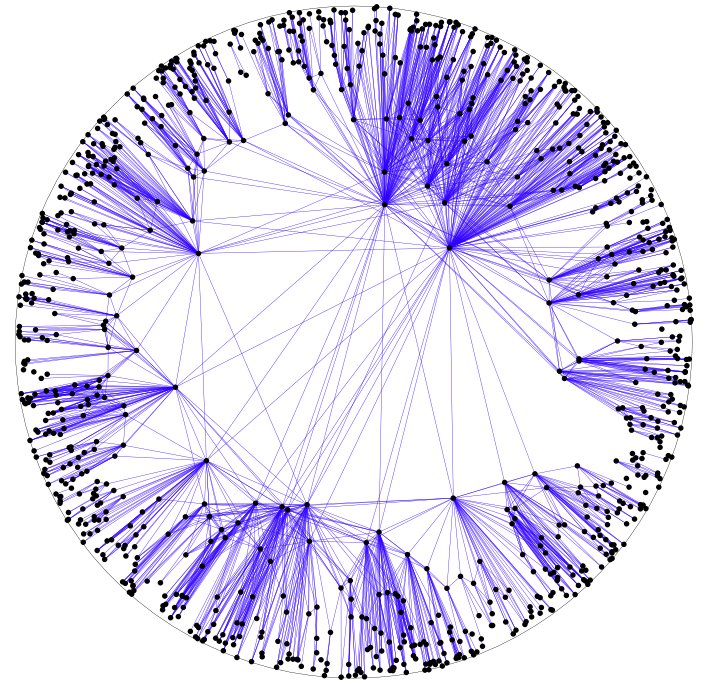
\includegraphics[scale=0.3]{figures/KPKVB.png}
\caption{Simulation $G(n;\alpha, \nu)$ with $\alpha = 0.9$, $\nu = 0.2$ and $n = 5000$.
%\PvdH{@Tobias: this figure (HyperRGG\_N5000L5.eps) is taken from the figures you send me. Could you fill in the value of $\alpha$ and $\nu$ you used for the simulation.}
}
\label{fig:H_graph_example}
\end{figure}

\noindent
Figure~\ref{fig:H_graph_example} shows a computer simulation of $G(n;\alpha, \nu)$.


As observed by Krioukov et al.~\cite{krioukov2010hyperbolic}, and proved rigorously by Gugelmann et al.~\cite{gugelmann2012random}, the degree sequence of the KPKVB model follows a power-law with exponent $2\alpha+1$.
% More specifically, if $N_k$ denotes the number of vertices of degree exactly $k$ then Gugelmann et al.~\cite{gugelmann2012random} have shown that
% 
% \begin{equation}\label{eq:gugeldegseq} 
% N_k = (1+o(1)) \cdot n \cdot p_k \quad \text{ a.a.s., }
% \end{equation}
% 
% \noindent
% where $p_k := 2\alpha \cdot \xi^{2\alpha} \cdot \Gamma^+\left(k - 2\alpha, \xi\right) / k!$
% with, here and in the rest of the paper, $\xi := \frac{4\alpha\nu}{\pi(2\alpha-1)}$ and 
% $\Gamma^+(a,b) := \int_b^\infty t^{a-1} e^{-t} \text{d}t$ the 
% {\em upper incomplete gamma function} and, for $(E_n)_n$ a sequence of events, 
% $E_n$ {\em asymptotically almost surely} (a.a.s.) means that $\Pee(E_n)\to 1$.
%%In particular $X_n = (1+o(1)) Y_n$ is equivalent to $X_n/Y_n \plim 1$.
%In fact~\eqref{eq:gugeldegseq} was shown in~\cite{gugelmann2012random} to hold not only when $k$ is constant but 
%also if $k$ depends on $n$ as long as $k = o( n^\delta )$ for a suitable small constant $\delta = \delta( \alpha )$.
%Standard asymptotic manipulations show that 
%
%$$p_k \sim 2\alpha\xi^{2\alpha} k^{-(2\alpha+1)}, $$
%
%as $k\to\infty$.
%\TM{ \RD{We need to add something like the following} : 
%In Appendix~\ref{} we settle the minor technical point of showing that~\eqref{eq:gugeldegseq} in fact extends 
%to all $k$ with $k \ll n^{1/(2\alpha+1)}$, while 
%$N_k = 0$ a.a.s.~whenever $k \gg n^{1/(2\alpha+1)}$. }
Gugelmann et al.~\cite{gugelmann2012random} also showed that the average degree converges in probability to the constant $8\nu\alpha^2/ \pi (2\alpha-1)^2$, and they showed that the (local) clustering coefficient is non-vanishing in the sense that it is bounded below by a positive constant a.a.s. Here, and in the rest of the paper, for a sequence $(E_n)_n$ of events, $E_n$ {\em asymptotically almost surely} (a.a.s.) means that $\Pee(E_n)\to 1$ as $n \to \infty$.
%Their work however left open the question of whether the clustering coefficient actually converges in probability.

Apart from the degree sequence and clustering, the third main characteristic associated with complex networks, ``short distances'', has also been established in the literature. In~\cite{abdullah2017typical} it is shown that for $\alpha < 1$ the largest component is what is called an \emph{ultra-small world}: if we randomly sample two vertices of the graph then, a.a.s., conditional on them being in the same component, their graph distance is of order $\log\log n$. In~\cite{kiwi2015bound} and~\cite{friedrich2018diameter} a.a.s.~polylogarithmic upper and lower bounds on the graph diameter of the largest component are shown, and in~\cite{muller2017diameter}, these were sharpened to show that $\log n$ is the correct order of the diameter.

Earlier work of the first and third authors with Bode~\cite{bode2015largest} and of the first and third authors~\cite{fountoulakis2018law} has established the ``threshold for a giant component'': if $\alpha < 1$ then there is a unique component of size linear in $n$ no matter how small $\nu$ (i.e. the average degree); if $\alpha > 1$ all components are sublinear no matter the value of $\nu$; and if $\alpha=1$ then there is a critical value $\nu_{\text{c}}$ such that for $\nu < \nu_{\text{c}}$ all components are sublinear and for $\nu > \nu_{\text{c}}$ there is a unique linearly sized component (all of these statements holding a.a.s.). Whether or not there is a giant component if $\alpha=1$ and $\nu=\nu_{\text{c}}$ remains an open problem. In~\cite{kiwi2015bound} and~\cite{kiwi2017second}, Kiwi and Mitsche considered the size of the second largest component and showed that for $\alpha \in (1/2, 1)$, a.a.s., the second largest component has polylogarithmic order with exponent $1/(\alpha -1/2)$.


In another paper of the first and third authors with Bode~\cite{bode2016probability} it was shown that $\alpha=1/2$ is the threshold for connectivity: for $\alpha < 1/2$ the graph is a.a.s.~connected, for $\alpha>1/2$ the graph is a.a.s.~disconnected and when $\alpha=1/2$ the probability of being connected tends to a continuous, nondecreasing function of $\nu$ which is identically one for $\nu \geq \pi$ and strictly less than one for $\nu < \pi$. Friedrich and Krohmer~\cite{blasius2018cliques} studied the size of the largest clique as well as the number of cliques of a given size. Bogu\~{n}a et al.~\cite{boguna2010sustaining} and Bl\"asius et al.~\cite{blasius2018efficient} considered fitting the KPKVB model to data using maximum likelihood estimation. Kiwi and Mitsche~\cite{kiwi2018spectral} studied the spectral gap and related properties, and Bl\"asius et al.\cite{blasius2016hyperbolic} considered the tree-width and related parameters of the KPKVB model. Recently Owada and Yogeshwaran~\cite{owada2018sub} considered subgraph counts, and in particular established a central limit theorem for the number of copies of a fixed tree $T$ in $G(n;\alpha,\nu)$, subject to some restrictions on the parameter $\alpha$.

\subsubsection*{Clustering}

In this work we study the clustering coefficient in the KPKVB model. In the literature there are unfortunately two distinct, rival definitions of the {\em clustering coefficient}. One of those, sometimes called the {\em global} clustering coefficient, is defined as three times the ratio of the number of triangles to the number of paths of length two in the graph. Results for this version of the clustering coefficient in the KPKVB model were obtained by Candellero and the first author~\cite{candellero2016clustering} and for the evolution of graphs on more general spaces with negative curvature by the first author in~\cite{fountoulakis2012evolution}. 

We will study the other notion of clustering, the one which is also considered by Krioukov et al.~\cite{krioukov2010hyperbolic} and Gugelmann et al.~\cite{gugelmann2012random}. It is sometimes called the {\em local} clustering coefficient, although we should point out that Gugelmann et al.~actually call it the global clustering coefficient in their paper. For a graph $G$ and a vertex $v\in V(G)$ we define the clustering coefficient {\em of $v$} as:
\[
	c(v) := \left\{\begin{array}{cl}
		\displaystyle \frac{1}{{\text{deg}(v)\choose 2}} \sum_{u,w\sim v} 1_{\{uw \in E(G)\}}, 
			& \text{ if $\text{deg}(v) \geq 2$, }\\
		& \\
        0, & \text{ otherwise,}
        \end{array}\right.
\]
where $E(G)$ denotes the edge set of $G$ and $\text{deg}(v)$ is the degree of vertex $v$. That is, provided $v$ has degree at least two, $c(v)$ equals the number of edges that are actually present between the neighbours of $v$ divided by the number of edges that could possibly be present between the neighbours given the degree of $v$.
The clustering coefficient of $G$ is now defined as the average of $c(v)$ over all vertices $v$:
\[
	c(G) := \frac{1}{|V(G)|} \sum_{v\in V(G)} c(v).
\]

As mentioned above, Gugelmann et al.~\cite{gugelmann2012random}, have established that $c(G(n;\alpha,\nu))$ is non-vanishing a.a.s., but they left open the question of convergence. Theorem~\ref{thm:maincc} below establishes that the clustering coefficient indeed converges in probability to a constant $\gamma$ that we give explicitly as a closed form expression involving $\alpha,\nu$ and several classical special functions.

In addition to the clustering coefficient, we shall also be interested in the {\em clustering function}.
This assigns to each non-negative integer $k$ the value
\begin{equation}\label{eq:def_clustering_function}
	c(k; G) := \begin{cases}
		\displaystyle \frac{1}{N(k)} \sum_{v \in V(G), \atop \text{deg}(v)=k}  c(v),  &\mbox{ if } N(k) \ge 1,\\
		0, &\mbox{else,}
	\end{cases}
\end{equation}
where $N(k)$ denotes the number of vertices of degree exactly $k$ in $G$. In other words, the clustering function assigns to the integer $k$ the average of the local clustering coefficient over all vertices of degree $k$. We remark that, while it might seem natural to consider $c(k)$ to be ``undefined'' when $N(k)=0$, we prefer to use the above definition for technical 
convenience.  This way $c(k; G(n;\alpha,\nu) )$ is a plain vanilla random variable and we can for instance compute its moments without any issues.

A general expression of the clustering function for KPKVB random graphs is given in~\cite[Equation (59)]{krioukov2010hyperbolic}. The authors conjecture that as $k$ tends to infinity, the clustering function decays as $k^{-1}$. They based this prediction on observations (Figure 8 in \cite{krioukov2010hyperbolic}) in experiments on the infrastructure of the Internet obtained in~\cite{claffy2009internet}. Despite these interesting observations and the attention the KPKVB model has generated since then, the behaviour of the clustering function in KPKVB random graphs had not been completely determined. In particular it has not been established whether it converges as $n\to\infty$ to some suitable limit function, nor how $c(k;G)$ scales with $k$. Theorems~\ref{thm:mainkfixed},~\ref{thm:mainktoinfty} and Proposition~\ref{prop:asymp} below settle these questions. Theorem~\ref{thm:mainkfixed} shows that for each fixed $k$, the value $c(k;G(n;\alpha,\nu))$ converges in probability to a constant $\gamma(k)$ that we again give explicitly as a closed form expression involving $\alpha,\nu$ and several classical special functions. Theorem~\ref{thm:mainktoinfty} extends this result to growing sequences satisfying $k \ll n^{1/(2\alpha+1)}$. Proposition~\ref{prop:asymp} clarifies the asymptotic behavior of the limiting function $\gamma(k)$, as $k\to\infty$. This depends on the parameter $\alpha$, and $\gamma(k)$ only scales with $k^{-1}$ when $\alpha > 3/4$, which corresponds to the exponent of the degree distribution exceeding $5/2$. 
So in particular our findings disprove the abovementioned conjecture of Krioukov et al.~\cite{krioukov2010hyperbolic}.


\subsubsection*{Notation}

In the statement of our main results, and throughout the rest of the paper, we will use the following notations. 
We set 
$$\xi := \frac{4\alpha\nu}{\pi(2\alpha-1)}. $$

We write $\Gamma(z) := \int_0^\infty t^{z-1} e^{-t}\text{d}t$ for the gamma function, 
$\Gamma^+(a,b) := \int_b^\infty t^{a-1} e^{-t}\text{d}t$ for the upper incomplete gamma function, 
 $B(a,b) := \int_0^1 u^{a-1}(1-u)^{b-1}\text{d}u = \Gamma(a)\Gamma(b) / \Gamma(a+b)$ for the beta function and 
 $B^-(x ; a,b) := \int_0^x u^{a-1}(1-u)^{b-1}\text{d}u$ for the lower incomplete beta function. 
We write $U(a,b,z)$ for the hypergeometric U-function (also called Tricomi's confluent hypergeometric function), which 
%for $a,b,z\in \mathbb{C}$, $b \not \in \mathbb{Z}_{\leq 0}$, $\mathrm{Re}(a), \mathrm{Re}(z) >0$ 
has the integral representation 
\[
	U(a,b,z) = \frac{1}{\Gamma(a)} \int_0^\infty e^{-zt} t^{a-1} (1+t)^{b-a-1} dt,
\] 
see~\cite[p.255 Equation (2)]{erdelyi1953higher}, and let $\MeijerGnew{m}{\ell}{p}{q}{{\bf a}}{{\bf b}}{z}$ denote 
Meijer's G-Function~\cite{meijer1946gfunction}, see Appendix~\ref{sec:Meijer_G_functions} for more details.

For a sequence $(X_n)_n$ of random variables, we write $X_n \xrightarrow[n\to\infty]{\Pee} X$ to denote that $X_n$ converges in probability to $X$, as $n \to \infty$.

%We further adopt standard notations on asymptotic behavior of functions and sequences. That is, for two functions $f$ and $g$, we write $f(n) = \smallO{g(n)}$ as $n \to \infty$ if $\limsup_{n \to \infty} f(n)/g(n) = 0$ and $f(n) = \bigO{g(n)}$ as $n \to \infty$ if $\limsup_{n \to \infty} |f(n)|/g(n) < \infty$. Furthermore, $f(n) = \Omega(g(n))$ as $n \to \infty$ if $\limsup_{n \to \infty} |f(n)/g(n)| > 0$ and $f(n) = \omega(g(n))$ as $n \to \infty$ if $\limsup_{n \to \infty} |f(n)/g(n)| = \infty$. Finally, $f(n) = \bigT{g(n)}$ as $n \to \infty$ if $f(n) = \bigO{g(n)}$ and $g(n) = \Omega(f(n))$.

 %In addition, $X_n \xrightarrow[n\to\infty]{L^1} X$ denotes convergence in expectation, i.e. $\Exp{|X_n - X|} \to 0$ as $n \to \infty$, which is a stronger notion than convergence in probability.

\subsection{Main results}\label{ssec:main_results}


\subsubsection{The clustering coefficient}

Our first result is the following.

\begin{theorem}\label{thm:clustering_coefficient_hyperbolic}\label{thm:maincc}
Let $\alpha > \frac{1}{2}$, $\nu > 0$ be fixed. Writing $G_n := G(n;\alpha,\nu)$, we have
\[
	c( G_n ) \xrightarrow[n\to\infty]{\Pee} \gamma,
\]
where $\gamma$ is defined for $\alpha \ne 1$ as
\begin{align*}
	\gamma 
	&=\frac{2 + 4 \alpha + 13 \alpha^2 - 34 \alpha^3 - 12\alpha^4 + 24 \alpha^5}{16(\alpha-1)^2 \alpha (\alpha+1) (2\alpha+1)} 
		+  \frac{2^{-1 - 4 \alpha}}{(\alpha - 1)^2} \\
&\hspace{10pt}+ \frac{(\alpha - 1/2) (B(2 \alpha, 2 \alpha + 1) + B^-(1/2; 1 + 2 \alpha, -2 + 2 \alpha))}{2 (\alpha - 1) (3 \alpha - 1)} \\
%
&\hspace{10pt}+ \frac{\xi^{2\alpha} \left( \Gamma^+( 1 - 2 \alpha, \xi) + \Gamma^+( - 2 \alpha, \xi)\right) }{4(\alpha-1)} \\
%
&\hspace{10pt}+ \frac{\xi^{2\alpha + 2}\alpha (\alpha - 1/2)^2 \left( \Gamma^+(- 2 \alpha - 1, \xi) + \Gamma^+(- 2 \alpha - 2, \xi)\right)}%
{2(\alpha-1)^2} \\
%
&\hspace{10pt}- \frac{\xi^{2\alpha + 1}\alpha (2\alpha - 1) \left( \Gamma^+( - 2\alpha,\xi)+\Gamma^+( - 2 \alpha - 1,\xi) \right)}%
{(\alpha-1)} \\
%
&\hspace{10pt}- \frac{\xi^{6\alpha-2}2^{-4\alpha}(3\alpha - 1)
\left( \Gamma^+( - 6 \alpha + 3, \xi)+\Gamma^+( - 6 \alpha + 2, \xi) \right)}{(\alpha-1)^2}\\
%
&\hspace{10pt}- \frac{\xi^{6\alpha - 2}(\alpha - 1/2) B^-(1/2; 1 + 2 \alpha, -2 + 2 \alpha)%
\left(\Gamma^+( - 6 \alpha + 3, \xi)+\Gamma^+( - 6 \alpha + 2, \xi)\right)}{(\alpha-1)} \\
%
&\hspace{10pt}- \frac{e^{-\xi} \Gamma(2\alpha+1) \left(U(2\alpha+1,1-2\alpha,\xi) + U(2\alpha+1,2-2\alpha,\xi)\right)}{4(\alpha-1)} \\
%
&\hspace{10pt}+ \frac{\xi^{6\alpha - 2} \Gamma(2\alpha+1)\left( \MeijerGnew{3}{0}{2}{3}{1,3-2\alpha}{3-4\alpha,-6\alpha+2,0}{\xi}
 		+ \MeijerGnew{3}{0}{2}{3}{1,3-2\alpha}{3-4\alpha,-6\alpha+3,0}{\xi}\right)}{4(\alpha-1)},
\end{align*}
and for $\alpha = 1$ as the $\alpha\to 1$ limit of the above expression. 
% \begin{align*}
% 	c_\infty &= \frac{575 - 12 \pi^2}{576} + \frac{\eta^4(7 + \pi^2)\Gamma^\ast(-4, \eta)}{4}\\
% 	&\hspace{10pt}- \frac{1}{2} \int_0^1 (1 - 4z + 3z^3)\log(1-z)(z + \eta)e^{-\eta/z} \dd z\\
% 	&\hspace{10pt}- \int_0^1 \Li_2(z)(z^3 + \eta z^2) e^{-\eta/z} \dd z,		
% \end{align*}
% with $\eta = 4\nu/\pi$ and $\Li_2(z) = \sum_{t = 1}^\infty z^t/t^2$, the dilogarithm function\footnote{Note that the integrals in the expression for $c_\infty$ for $\alpha = 1$ exists: for the first one note that $1-4z+3z^2=(1-z)(1-3z)$, so the integrand can be bounded by $C(1-z)\log(1-z)$ on $[0,1)$ for some constant $C$, which can be continued continuously to the compact interval $[0,1]$ by noting that the limit for $z \rightarrow 1$ is zero, so the integrand is bounded on a bounded domain and hence, this integral is finite; for the second integral note that $\Li_2(z)$ is bounded by $\Li_2(1)$ on $[0,1]$, which is a series with well-known finite limit, so again the integrand is bounded on a bounded domain and hence the second integral is also finite.}.
\end{theorem}

\noindent
A plot of $\gamma$ can be found in Figure~\ref{fig:gamma}.


\begin{figure}[h!]
    \centering
    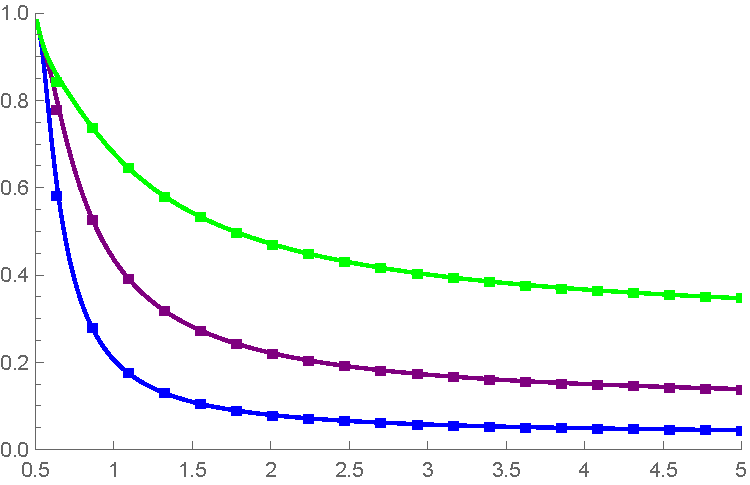
\includegraphics[scale=0.6]{figures/cn10000nu0512rep100a05to5Squares.pdf}
    \caption{Plot of $\gamma$ for $\alpha$ varying from $0.5$ to $5$ on the horizontal axis and 
    for $\nu=\frac{1}{2}$ (blue), $\nu=1$ (purple), $\nu=2$ (green); simulations (squares in corresponding colour) with $n=10000$ and $100$ repetitions.\label{fig:gamma}}
\end{figure}

In the above expression for $\gamma$, a factor $\alpha-1$ occurs in the denominator of each term, but we will see that this
corresponds to a removable singularity. We have not been able to find a closed form expression in terms of known functions in the case when $\alpha=1$, but in Section~\ref{ssec:alphais1} we do provide an explicit expression involving integrals.


\subsubsection{The clustering function}

Our second result is on the clustering function for constant $k$.

\begin{theorem}\label{thm:local_clustering_hyperbolic}\label{thm:mainkfixed}
Let $\alpha > \frac{1}{2}$, $\nu > 0$ and $k\geq2$ be fixed. 
Writing $G_n := G(n;\alpha,\nu)$, we have

\[
	c(k;G_n) \xrightarrow[n\to\infty]{\Pee} \gamma(k),
\]
where $\gamma(k)$ is defined for $\alpha \ne 1$ as 
\begin{align*}
\gamma(k)  =&\frac{1}{8\alpha (\alpha-1)\Gamma^+(k-2\alpha,\xi)} \left( -\Gamma^+(k - 2 \alpha, \xi) - 2\frac{\alpha (\alpha - 1/2)^2 \xi^{2} \Gamma^+(k - 2 \alpha - 2, \xi)}{(\alpha - 1)} \right. \\ 
&\left.+ 8 \alpha (\alpha - 1/2) \xi \Gamma^+(k - 2 \alpha - 1,\xi) \right.\\ 
&\left.+ 4\xi^{4\alpha - 2} \Gamma^+(k - 6 \alpha + 2, 
      \xi) \left( \frac{2^{ - 4\alpha}(3 \alpha - 1)}{(\alpha - 1)} + (\alpha - 1/2) B^-(1/2; 1 + 2 \alpha, -2 + 2 \alpha) \right)  \right.\\ 
&\left.+ \xi^{k-2\alpha} \Gamma(2\alpha+1)e^{-\xi} U(2\alpha+1,1+k-2\alpha,\xi) \right. \\ 
&\left.- \xi^{4\alpha-2} \Gamma(2\alpha+1)\MeijerGnew{3}{0}{2}{3}{1,3-2\alpha}{3-4\alpha,-6\alpha+k+2,0}{\xi}  \right)
\end{align*}
and for $\alpha = 1$ as the $\alpha\to1$ limit of the above expression.
% \begin{align*}
% 	c_\infty(k) &= \frac{9 \eta^3}{2 k!} 	
% 		\Gamma^+(k-3,\eta)-\frac{\xi^4}{k!}\frac{7+\pi^2}{4}\Gamma^+(k-4,\eta)\\
% 	&\hspace{10pt}+ \frac{\eta^k}{2k!}\int_0^1 (1-4z+3z^2)\ln(1-z)z^{1-k}e^{-\eta/z}\dd z\\ 
% 	&\hspace{10pt}+ \frac{\eta^k}{k!}\int_0^1 z^{3-k} \Li_2(z) e^{-\eta/z} \dd z,
% \end{align*}
% with $\eta = 4\nu/\pi$ and $\Li_2(z) = \sum_{t = 1}^\infty z^t/t^2$, the dilogarithm function.
\end{theorem}

\noindent
A plot of $\gamma(k)$ can be found in Figure~\ref{fig:gammak}. %
%
%
\begin{figure}[h!]
    \centering
    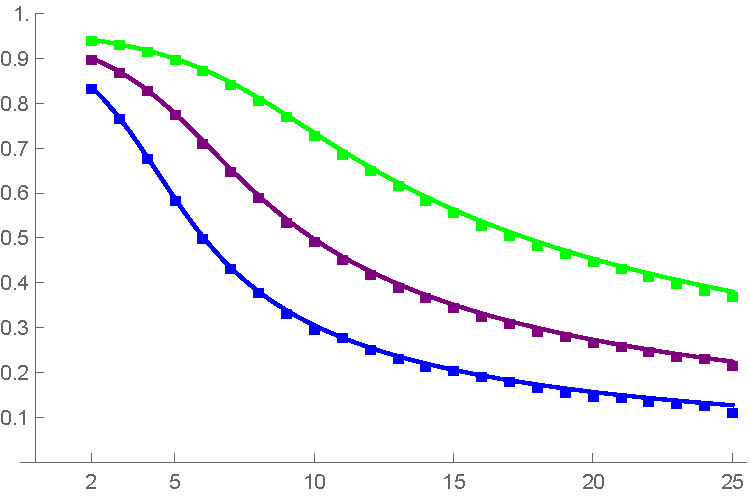
\includegraphics[scale=0.6]{figures/ckn10000a08nu0512rep100k2to25Squares.pdf}
    \caption{Plot $\gamma(k)$ for $k$ varying from 2 to 25 on the horizontal axis, for $\alpha=0.8$ and $\nu=\frac{1}{2}$ 
    (blue), $\nu=1$ (purple), $\nu=2$ (green); simulations (squares in corresponding colour) with $n=10000$ and $100$ repetitions.\label{fig:gammak}}
\end{figure}%
%
Again, we remark that the above expression for $\gamma(k)$ appears to have a singularity at $\alpha=1$, but this will turn out to be a removable singularity. Again, we have not been able to find a closed form expression in terms of known functions in the case when $\alpha=1$, but in Section~\ref{ssec:alphais1} we do provide an explicit expression involving integrals.

Theorem~\ref{thm:mainkfixed} in fact generalises to increasing sequences $(k_n)_{n \ge 1}$.

\begin{theorem}\label{thm:mainktoinfty}
Let $\alpha>\frac12, \nu>0$ be fixed and let $k_n$ be a sequence of integers
satisfying $1 \ll k_n \ll n^{1/(2\alpha+1)}$. Then, writing $G_n := G(n;\alpha,\nu)$, we have
\[
	\E[|c(k_n;G_n)-\gamma(k_n)|] = \smallO{\gamma(k_n)},
\]
as $n \to \infty$, where $\gamma(\cdot)$ is as in Theorem~\ref{thm:mainkfixed}. In particular
\[
	\lim_{n \to \infty} \Exp{\left|\frac{c(k_n; G_n)}{\gamma(k_n)}- 1 \right|} = 0.
\]
\end{theorem}

%We remark that the number of vertices of degree exactly $k$ satisfies $N_k = 0$ a.a.s.~when $k \gg n^{1/(2\alpha+1)}$, see~\TM{ add reference to correct thm / lemma here! }.
%So the range in the above result is essentially to best possible.

\subsubsection{Scaling of $\gamma(k)$}

To clarify the scaling behaviour of $\gamma(k)$ with $k$ we offer the following result.

\begin{proposition}\label{prop:asymp}
As $k\to\infty$, we have

$$ \gamma(k) = 
(1+o(1)) \cdot \left\{ \begin{array}{cl}
\frac{8\alpha \nu}{\pi\left(4\alpha - 3\right)} \cdot k^{-1} &\text{ if } \alpha > \frac{3}{4}, \\
\frac{6 \nu}{\pi} \cdot \frac{\log(k)}{k}& \text{ if } \alpha = \frac{3}{4},\\
 c_{\alpha} \cdot k^{2-4\alpha} & \text{ if } \frac12 < \alpha < \frac34, 
\end{array} \right.,
$$
where $c_{\alpha} := \left( \frac{3\alpha - 1}{2^{4\alpha+1}\alpha(\alpha-1)^2} 
	+ \frac{(\alpha - \frac{1}{2})B^-(\frac{1}{2},2\alpha + 1, 2\alpha - 2)}{2(\alpha - 1)\alpha} 
	- \frac{B(2\alpha, 3\alpha - 4)}{4(\alpha - 1)} \right)  \cdot \xi^{4\alpha-2}$.
\end{proposition}

Note that Theorem~\ref{thm:mainktoinfty} implies that the clustering function of the KPKVB model scales as $\gamma(k)$ as $k$ grows, whose scaling is given in the above result. In particular, this contradicts the scaling conjectured in~\cite{krioukov2010hyperbolic} for $\alpha \leq \frac34$, and confirms it only for $\alpha > \frac34$.

We remark that simultaneously and independently Stegehuis, van der Hofstad and van Leeuwaarden~\cite{stegehuis2018scale} found a similar, but less detailed result on the $k\to\infty$ scaling of the clustering function in the KPKVB model.

\subsection{Observations}

There are a few other observation to be made regarding our results.

\paragraph{Uniform convergence.}

Our results for the local clustering function in particular imply uniform convergence of $c(k; G_n)$ for all $2 \le k \le a_n$ where $a_n \ll n^{\frac{1}{2\alpha + 1}}$. To see this let
\[
	b_n = \arg \max_{2 \le k \le a_n} \Exp{\left|\frac{c(k_n; G_n)}{\gamma(k)} - 1\right|}.
\]
Then $b_n \le a_n \ll n^{\frac{1}{2\alpha + 1}}$ and therefore by Theorem~\ref{thm:local_clustering_hyperbolic}
\[
	\lim_{n \to \infty} \max_{2 \le k \le a_n} \Exp{\left|\frac{c(k; G_n)}{\gamma(k)} - 1\right|} 
	= \lim_{n \to \infty}\Exp{\left|\frac{c(b_n; G_n)}{\gamma(b_n)} - 1\right|} = 0.
\]


\paragraph{Near maximum scaling for $k_n$.}
Our results for the clustering function in the KPKVB model are valid for any sequence of integers $k_n \to \infty$ such that $k_n \ll n^{\frac{1}{2\alpha + 1}}$. Although one would like to have results for any sequence $k_n \le n$, it turns out that $n^{1/(2\alpha + 1)}$ is the near maximum scaling for which Theorem~\ref{thm:clustering_coefficient_hyperbolic} can be true. To see why this is the case note that by definition of the local clustering function~\eqref{eq:def_clustering_function} we have that $c(k_n; G_n) = 0$ if $N_{n}(k_n) = 0$, where $N_n(k_n)$ denote the number of vertices in a KPKVB graph $G(n; \alpha, \nu)$ with degree $k_n$. It follows by Markov's inequality that for any positive function $f : \R_+ \to \R_+$
\begin{align*}
	\Exp{\left|\frac{c(k_n; G_n)}{f(k_n)} - 1\right|} 
	&\ge \Exp{\left|\frac{c(k_n; G_n)}{f(k_n)} - 1\right|\ind{N_n(k_n) = 0}}\\ 
	&\ge \Prob{N_{n}(k_n) = 0} \ge 1 - \Exp{N_n(k_n)}.
\end{align*}
We shall later establish (see Lemma~\ref{lem:diff_Nk_hyperbolic_binomial_poisson}) that $\Exp{N_n(k_n)}$ scales as $n k_n^{-(2\alpha + 1)}$. Therefore if $k_n$ is such that $k_n^{-(2\alpha + 1)} n$ tends to zero as $n \to \infty$ we have that 
\[
	\lim_{n \to \infty} \Exp{N_{n}(k_n)} = 0
\]
and hence
\[
	\lim_{n \to \infty} \Exp{\left|\frac{c(k_n; G_n)}{f(k_n)} - 1\right|} 
	\ge 1 - \lim_{n \to \infty} \Exp{N_{n}(k_n)} = 1 \ne 0,
\]
for any positive function $f$. This implies that we cannot expect a result like that of Theorem~\ref{thm:mainktoinfty} to hold as soon as $k_n \gg n^{\frac{1}{2\alpha + 1}}$.

\paragraph{Transition in scaling at $\bm{\alpha = 3/4}$.}

\PvdH{We should try and add something here. Not necessarily needed for the submission to arXiv though.}

\subsection{Outline of the paper}


In the next section we will recall some useful tools from the literature and define a series of auxiliary random graph models that will be used in the proofs. In particular, we relate in a series of steps the KPKVB model to an infinite percolation model $\Ginf$ that was used in previous work of the first and third authors~\cite{fountoulakis2018law} on the largest component of the KPKVB model. The value of the limiting constant $\gamma$, respectively limiting clustering function $\gamma(k)$, correspond to the probability that two randomly chosen neighbours of a ``typical point'' in this infinite model are themselves neighbours, respectively the probability of this event conditional on the typical point having exactly $k$ neighbours. These probabilities can be expressed as certain integrals, which we solve explicitly in Section~\ref{sec:Ginf}. 
In the same section we also prove Proposition~\ref{prop:asymp}, on the asymptotics of $\gamma(k)$. We then proceed to prove Theorems~\ref{thm:maincc} and~\ref{thm:mainkfixed} by relating said probabilities for the typical point of the infinite model to the corresponding clustering coefficient/function in the original KPKVB random graph, using the Campbell-Mecke formula and some other, relatively straightforward considerations.

The remaining sections are devoted to the proof of Theorem~\ref{thm:mainktoinfty}, which turns out to be a lot more involved. The main reason for this is that we push the possible scaling of $k_n$ to its maximum and hence a great deal of work is needed to properly control the arising error terms and make sure these are of smaller order than $\gamma(k_n)$. 

Finally, the Appendix includes some technical results on Meijer's G-function, Chernoff bounds for Poisson and Binomial random variables and the code used for simulations.




\section{Preliminaries\label{sec:proof_outline}}

In this section we recall some definitions and tools that we will need in our proofs.

\subsection{The infinite limit model $\Ginf$\label{ssec:infinite_model}}

We start by recalling the definition of the infinite limit model from~\cite{fountoulakis2018law}.
Let $\mathcal{P}=\mathcal{P}_{\alpha,\nu}$ be a Poisson point process on $\eR^2$ with intensity function $f=f_{\alpha,\nu}$ given by

\begin{equation}\label{eq:def_intensity_function_f}
	f(x,y) = \frac{\alpha \nu}{\pi} e^{-\alpha y} \cdot \1_{\{y>0\}}.
\end{equation} 

The \emph{infinite limit model} $\Ginf = \Ginf(\alpha,\nu)$ has vertex set $\mathcal{P}$ and edge set such that
\[
	pp' \in E(\Ginf) \iff |x - x'| \leq e^{\frac{y + y'}{2}},
\]
for $p=(x,y),p'=(x',y')\in\Pcal$.

For any point $p \in \R \times (0,\infty)$, we write $\BallPo{p}$ to denote the \emph{ball} around $p$, i.e.

\begin{equation}\label{eq:def_ball_P}
	\BallPo{p} = \{p^\prime \in \eR\times(0,\infty) : |x - x^\prime| \leq e^{\frac{y + y^\prime}{2}}\}.
\end{equation}

With this notation we then have that $\BallPo{p} \cap \Pcal$ denotes the set of neighbours of a vertex $p \in \Ginf$.
We will denote the intensity measure of the Poisson process $\mathcal{P}$ by $\mu = \mu_{\alpha, \nu}$, i.e. for every 
Borel-measurable subset $S \subseteq \eR^2$ we have $\mu(S) = \int_S f(x,y) \dd x \dd y$. Using the notation $p = (x,y)$ for a point in $\R \times \R_+$ we shall write $\int_S h(p) \dd \mu(p)$ for the integral of $h$ over $S$ with respect to the intensity measure $\mu$, i.e. $\int_S h(p) \dd \mu(p) = \int_{S} h(x,y) f(x,y) \dd x \dd y$.


\subsection{The finite box model $\Gbox$\label{ssec:finite_model}}


Recall that in the definition of the KPKVB model we set $R = 2\log(n/\nu)$.
We consider the box $\Rcal = (-\frac{\pi}{2}e^{R/2}, \frac{\pi}{2}e^{R/2}] \times (0, R]$ in $\eR^2$. 
Then the \emph{finite box model} $\Gbox = \Gbox(n;\alpha, \nu)$ has vertex set $\Vbox := \mathcal{P} \cap \Rcal$ and edge set such that
\[
	pp' \in E(\Gbox) \iff |x - x'|_{\pi e^{R/2}} \leq e^{\frac{y + y'}{2}},
\]
where $|x|_{r} = \min( |x|, r - |x|)$ for $-r\leq x\leq r$. Using $|.|_{\pi e^{R/2}}$ instead of $|.|$ results in the left and right boundaries of the box $\Rcal$ getting identified, which in particular makes the model invariant under horizontal shifts and reflections in vertical lines. 
The graph $\Gbox$ can thus be seen as a subgraph of $\Ginf$ induced on $\Vbox$, with some additional edges caused by the identification of the boundaries.

Similar to the infinite graph, for a point $p \in \Rcal$ we define the ball $\BallPon{p}$ as
\begin{equation}\label{eq:def_ball_P_n}
	\BallPon{p} = 
	\left\{p' \in \Rcal : |x - x'|_{\pi e^{R/2}} \leq e^{\frac{y + y'}{2}}\right\}.
\end{equation}


\subsection{The Poissonized KPKVB model $\GPo$}


Imagine that we have an infinite supply of i.i.d.~points $u_1, u_2, \dots$ in the hyperbolic plane $\Haa$ chosen according to the $(\alpha, R)$-quasi uniform distribution. In the standard KPKVB random graph $G(n;\alpha,\nu)$ we take $u_1,\dots, u_n$ as our vertex set and add edges between points at hyperbolic distance at most $R = 2\log(n/\nu)$. In the \emph{Poissonized} KPKVB random graph $\GPo := \GPo(n;\alpha,\nu)$, we instead take $N\isd \Po(n)$, a Poisson random variable 
with mean $n$, independent of our i.i.d.~sequence of points and let the vertex set be $u_1,\dots, u_N$ and add edges 
according to the same rule as before. Equivalently, we could say that the vertex set consists of the points of a Poisson point process with intensity function $n g$, where $g$ denotes the probability density of the $(\alpha,R)$-quasi uniform distribution. That is,
\begin{equation}\label{eq:def_quasi_uniform_density}
	g(r,\theta) = \frac{\alpha\sinh(\alpha r)}{2\pi(\cosh(\alpha R) - 1)} \cdot 1_{\{0\leq r\leq R, -\pi<\theta\leq \pi\}}.
\end{equation}

Working with the Poissonized model has the advantage that when we take two disjoint regions $A, B$ then the number of points in $A$ and the number of points  in $B$ are independent Poisson-distributed random variables. As we will see, and as is to be expected, switching to the Poissonized model does not significantly alter the limiting behaviour of the clustering coefficient and function.


\subsection{Coupling $\GPo$ and $\Gbox$\label{ssec:coupling_H_P}}


The following lemmas from \cite{fountoulakis2018law} establish a useful coupling between the Poissonized KPKVB random graph
and the finite box model and relate the edge  sets of the two graphs. 

\begin{lemma}[{\cite[Lemma 27]{fountoulakis2018law}}]\label{lem:coupling_hyperbolic_poisson}
Let $\VPo$ denote the vertex set of $\GPo(n;\alpha, \nu)$ and $\Vbox$ the vertex set of $\Gbox(n;\alpha, \nu)$. 
Define the map $\Psi : [0,R] \times (-\pi, \pi] \to \Rcal$ by
\begin{equation}\label{eq:def_Psi}
	\Psi(r,\theta) = \left(\theta \frac{e^{R/2}}{2}, R - r\right).
\end{equation}
Then there exists a coupling such that, a.a.s., $\Vbox = \Psi[\VPo]$. %Moreover, if $\Ccal_n$ is the event that ${\cal V}_n = \Psi\left(\mathcal{V}_{\HP,n}\right)$ then
%\begin{equation}\label{eq:convergence_miscoupling_hyperbolic_poisson}
%	\Prob{\Ccal_n^c} = \bigO{n^{-(2\alpha - 1)}}. 
%\end{equation}
\end{lemma}

In the remainder of this paper we will write $\BallHyp{p}$ to denote the image under $\Psi$ of the ball of hyperbolic radius $R$ around the point 
$\Psi^{-1}(p)$ for $p \in \Rcal$, i.e. 
\[
	\BallHyp{p} := 
	%\left\{p^\prime := \Psi(u) \, : \, u \in \Dcal_{R} \text{ and } d_\H(\Psi^{-1}(p),u) \le R\right\}.
	\Psi\left[ \left\{ u \in \Haa : 
	d_\H(\Psi^{-1}(p),u), d_\H(O,u) \le R \right\}\right] \subset \Rcal.
\]

Under the map $\Psi$, a point $p = (x,y) \in \Rcal$ corresponds to $u := \Psi^{-1}(p) = (2 e^{-R/2} x, R - y)$. 

By the hyperbolic rule of cosines, for two points $p = (x,y) = \Psi( (r,\theta) ), p' = (x',y') = \Psi( (r',\theta') ) \in \Rcal$ we have that $p' \in \BallHyp{p}$ iff.~either $r+r'\leq R$ or $r+r'>R$ and
\[
	\cosh r \cosh r' - \sinh r \sinh r'\cos\left( |\theta-\theta'|_{2\pi} \right) \le \cosh(R),
\]
This can be rephrased as $p'\in \BallHyp{p}$ iff.~either $y+y'\geq R$ or $y+y'<R$ and 


\begin{equation}\label{eq:def_Omega_hyperbolic}
	|x-x'|_{\pi e^{R/2}} \leq \Phi(y,y^\prime) := \frac{1}{2}e^{R/2} \arccos\left( \frac{\cosh(R-y) \cosh(R-y^\prime) - \cosh R}{\sinh(R-y) \sinh(R-y^\prime)} \right).
\end{equation}

The following lemma provides useful bounds on the function $\Phi(r,r^\prime)$. Note that in~\cite{fountoulakis2018law} the function $\Phi$ is written in terms of where $r := R - y, r^\prime := R - y^\prime$. 

\begin{lemma}[{\cite[Lemma 28]{fountoulakis2018law}}]\label{lem:asymptotics_Omega_hyperbolic}
There exists a constant $K>0$ such that, for every $\varepsilon > 0$ and for $R$ sufficiently large, the following holds.
For every $r,r^\prime \in [\varepsilon R,R]$ with $y + y^\prime < R$ we have that 
\begin{equation}\label{eq:asymp1}
	e^{\frac{1}{2}(y+y^\prime)} - K e^{\frac{3}{2}(y+y^\prime) - R} \leq \Phi(y, y^\prime) 
	\leq  e^{\frac{1}{2}(y+y^\prime)} + K e^{\frac{3}{2}(y+y^\prime) - R},
\end{equation}
Moreover:
\begin{equation}\label{eq:asymp2} 
\Phi(y,y^\prime) \geq e^{\frac12(y+y^\prime)} \quad \text{if \quad $y, y^\prime > K$.} 
\end{equation}
\end{lemma}

A key consequence of Lemma~\ref{lem:asymptotics_Omega_hyperbolic} is that the coupling from Lemma~\ref{lem:coupling_hyperbolic_poisson} preserves edges between points whose heights are not too large.  

\begin{lemma}[{\cite[Lemma 30]{fountoulakis2018law}}]\label{lem:coupling_edges}
On the coupling space of Lemma~\ref{lem:coupling_hyperbolic_poisson} the following holds a.a.s.:
\begin{enumerate}
\item for any two points $p, p' \in \Vbox$ with $y, y'\le R/2$, we have 
\[
	pp' \in E(\Gbox) \Rightarrow \Psi^{-1}(p)\Psi^{-1}(p') \in E(\GPo),
\]
\item for any two points $p, p' \in \Vbox$ with $y, y' \le R/4$, we have that 
\[
	pp' \in E(\Gbox) \iff \Psi^{-1}(p)\Psi^{-1}(p') \in E(\GPo).
\]

\end{enumerate}
\end{lemma}

\begin{remark}[Notational convention for points]
We will often be working with the finite box graph $\GPo$ or the infinite graph $\Ginf$, whose nodes are points 
in $\R \times \R_+$. For any point $p \in \R \times \R_+$ we will always use $p = (x,y)$. 
When considering different points $p,p^\prime \in \R \times \R_+$, we will use primed coordinates to refer 
to $p^\prime$, i.e. $p^\prime = (x^\prime ,y^\prime)$, and similar with subscripts, i.e. $p_i = (x_i,y_i)$.
\end{remark}

\subsection{The Campbell-Mecke formula}

A useful tool for analyzing subgraph counts, and their generalizations, in the 
setting of Poissonized random geometric graphs, and in particular the Poissonized KPKVB model and the box 
model is the \emph{Campbell-Mecke formula}. 
We use a specific incarnation, which follows from the Palm theory of Poisson point processes on metric 
spaces, see~\cite{last2017lectures}. For this consider a Poisson point process $\Pcal$ on some metric 
space $\mathcal{M}$ with density $\mu$ and let $\mathcal{N}$ denote the set of all possible point configurations 
in $\mathcal{M}$, equipped with the sigma algebra of the process $\Pcal$. 
Then, for any natural number $k$ and measurable function $h : \R^k \times \mathcal{N} \to \R$,

\begin{equation}\label{eq:def_campbell_mecke}
\begin{array}{c}
\displaystyle	\Exp{\sum_{p_1, \dots, p_k \in \Pcal, \atop \text{distinct}} h(p_1, \dots, p_k, \Pcal)} \\
= \\
\displaystyle \int_{\mathcal{M}} \dots \int_{\mathcal{M}} \Exp{h(x_1,\dots, x_k, \Pcal\cup\{x_1,\dots,x_k\})} \mu(dx_1)\dots\mu(dx_k).
\end{array}
\end{equation}

\subsection{Concentration of heights}

When analyzing degrees and clustering in the Poissonized KPKVB and related models we often encounter expressions of the form
\begin{equation}\label{eq:example_poisson_integral}
	\int_{0}^R \Prob{\Po(\hat{\mu}(y)) = k_n} h(y) e^{-\alpha y} \dd y,
\end{equation}
where $h(y)$ is some function and $\hat{\mu}(y)$ is $\Mu{\BallHyp{y}}$, $\Mu{\BallPon{y}}$ or $\Mu{\BallPo{y}}$. We will often have to either bound the behavior of such integrals as $k_n \to \infty$ or establish their asymptotic behavior. For this we will utilize that Poisson random variables are well concentrated around their mean. 

Let $\Po(\lambda)$ denote a Poisson random variable with mean $\lambda$. Then we have the following Chernoff bound (c.f. \cite[Lemma 1.2]{penrose2003random})
\begin{equation}\label{eq:def_chernoff_bound_poisson}
	\Prob{\left|\mathrm{Po}(\lambda) - \lambda\right| \ge x} \le 2e^{-\frac{x^2}{2(\lambda + x)}}.
\end{equation}
In particular, if $\lambda = \lambda_n \to \infty$, then for any $C>0$,
\begin{equation}\label{eq:def_chernoff_bound_poisson_C}
	\Prob{\left|\mathrm{Po}(\lambda_n) - \lambda_n\right| \ge C \sqrt{\lambda_n\log(\lambda_n)}} \le \bigO{\lambda_n^{-\frac{C^2}{2}}}.
\end{equation}

For our application these Chernoff bounds imply that if $y$ is such that $\hat{\mu}(y)$ is far from $k_n$ then $\Prob{\Po(\hat{\mu}(y)) = k_n}$ becomes very small. To be more specific, we define for any $k \ge 0$ and $C > 0$,
\begin{equation}\label{eq:def_y_k_C}
	y_{k,C}^\pm = 2 \log\left(\frac{k \pm C \sqrt{k \log(k)}}{\xi}\right),
\end{equation}
where we set $y_{k,C}^- = 0$ if $k - C \sqrt{k \log(k)} < \xi$ and likewise if $k + C \sqrt{k \log(k)} < \xi$ we set $y_{k,C}^+=0$, but  note that as we consider $k\rightarrow\infty$, we can assume that this case does not occur. For convenience we write $\Kcal_C(k_n) := [y_{k_n,C}^-, y_{k_n,C}^+]$. Then we can show that for all $y$ outside $\Kcal_C(k_n)$
\begin{equation}\label{eq:chernoff_bound_degrees}
	\Prob{\Po(\hat{\mu}(y)) = k_n} \le \bigO{k_n^{-\frac{C^2}{2}}}.
\end{equation}
Since we can select $C$ to be as big as we want we can make this error as small as needed. This implies that then the main contribution to the integral~\eqref{eq:example_poisson_integral} comes from those `'heights" $y$ that are in the interval $\Kcal_C(k_n)$. In other words, the main contribution is concentrated around the heights $y$ for which $\mu(y) = k_n$. We thus refer to this as the concentration of heights result. More precisely, we prove the following.

\begin{proposition}[Concentration of heights]\label{prop:concentration_height_general}
Let $\alpha > \frac{1}{2}$, $\nu > 0$, $(k_n)_{n \ge 1}$ be any positive sequence such that $k_n \to \infty$ and $k_n = \smallO{n}$. Furthermore, let $\hat{\mu}(y)$ denoting either $\Mu{\BallHyp{y}}$, $\Mu{\BallPon{y}}$ or $\Mu{\BallPo{y}}$. Then for any continuous function $h : \R_+ \rightarrow  \R$, such that $h(y) = \bigO{e^{\beta y}}$ as $y \to \infty$ for some $\beta < \alpha$, it holds that
\begin{equation*}%\label{eq:error_bound_int_rho_not_K}
	\int_0^\infty \hspace{-3pt} h(y) \Prob{\Po(\hat{\mu}(y)) = k_n} \alpha e^{-\alpha y} \dd y
	\sim \int_{\Kcal_C(k_n)} \hspace{-8pt} h(y) \Prob{\Po(\hat{\mu}(y)) = k_n} \alpha e^{-\alpha y} \dd y,
\end{equation*}
as $n \to \infty$.
\end{proposition}


The key implication of Proposition~\ref{prop:concentration_height_general} is that if the function $h(y)$ does not increase too fast, then we can restrict integration to the interval $\Kcal_C(y)$. The full details associated with these concentration of heights and the proof of Proposition~\ref{prop:concentration_height_general} can be found in the Section~\ref{sec:concentration_argument} of the Appendix.

%To see this result in action consider the finite box model $\Gbox$. Then 
%\[
%	\Exp{\Nbox(k)} = \Exp{\sum_{p \in \Pcal} \ind{\Dbox(p) = k}}
%	= \int_\Rcal \Prob{\Dbox(p) = k} f(x,y) \dd x \dd y.
%\]
 
%
%
%We use the incarnation below, which can be found in the monograph~\cite{penrose2003random}, as Theorem 1.6.
%
%\PvdH{I found it extremely hard to see the implications of this theorem. I therefore strongly recommend using more explicit version, for instance as in the previous version of the paper, or explicitly state the consequences of this result which will be used here.}
%
%\begin{theorem}[\cite{penrose2003random}]\label{thm:palm}
%Let $\Qcal$ be a Poisson process on $\eR^d$ with intensity function $g$, and suppose that $\lambda := \int g < \infty$.
%Suppose that $h(\Ycal, \Xcal)$ is a bounded measurable function, defined on pairs $(\Ycal,\Xcal)$ with $\Ycal \subseteq \Xcal \subseteq \eR^d$
%and $\Xcal$ finite, such that $h(\Ycal,\Xcal) = 0$ whenever $|\Ycal| \neq j$ (for some $j \in \eN$).
%Then
%\[ \Ee \sum_{\Ycal \subseteq \Qcal} h( \Ycal, \Qcal) = \frac{\lambda^j}{j!} \cdot \Ee h(\{Y_1,\dots, Y_j\}, \{Y_1,\dots, Y_j\} \cup \Qcal ), \]
%\noindent
%where the $Y_i$ are i.i.d.~random variables that are independent of $\Pcal$ and have common probability density function
%$g/\lambda$.
%\end{theorem}

% Let $\mathcal{Q}$ be a point process on a metric space $S$ with density $\rho$. 
% Let $\mathcal{N} = \mathcal{N} (\mathcal{S})$ be the set of all countable point configurations in $\mathcal{S}$
% equipped with the $\sigma$-algebra of the point process (that is, for any open subset 
% $A\subseteq S$ and any non-negative integer $m$ define a basic measurable subset of 
% $\mathcal{N}$ which consists of all configurations which have exactly $m$ points in $A$). 
% Now, let $h : S^{k} \times \mathcal{N} \rightarrow \eR$ be a measurable function. 
% The Palm theory of Poisson point processes on metric spaces~\cite{bk:LastPenrose} yields: 
% 
% \begin{equation} \label{eq:Mecke}
% \E \left( \sum_{p_1, \ldots, p_k \in {\mathcal Q}, \atop \text{distinct}} h(p_1,\ldots, p_k, \mathcal{Q})  \right) =
% \int_S \cdots \int_S \E (h(x_1,\ldots, x_k, \mathcal{Q})) d\rho (x_1) \cdots d \rho (x_k),
% \end{equation} 
% 
% where the sum ranges over all those $k$-tuples of points which contain no repetitions. 
% Note that in the RHS, the points $x_1, \dots, x_k$ are not part of $\Qcal$.






\section{Clustering and the degree of the typical point in $\Ginf$\label{sec:Ginf}\label{sec:asymptotics_average_clustering_ast_P}}


As mentioned earlier, we plan to make use of the Campbell-Mecke formula for comparing the clustering coefficient and function of $\GPo$ with certain quantities associated with $\Ginf$. We will be considering the Poisson process $\Pcal$ to which we add one additinal point $(0,y)$ on the $y$-axis. In some computations the height $y$ will be fixed, but eventually we shall take it exponentially distributed with parameter $\alpha$, and independent of $\Pcal$.
We refer to $(0,y)$ as ``the typical point''.

To provide some intu\"{\i}tion for this definition and name, note that we can alternatively view $\Pcal$ as follows. 
We take a constant intensity Poisson process on $\eR$ corresponding to the $x$-coordinates, and to each point
we attach a random ``mark'', corresponding to the $y$-coordinate, where the marks are i.i.d.~exponentially distributed with parameter $\alpha$.


Since $c(G)$ is defined as an average over all vertices of the graph, it is not immediately obvious how to meaningfully define a corresponding notion for infinite graphs, and similarly for the clustering function, the degree sequence, etc.
We can however without any issues speak of the (expected) clustering coefficient of the typical point, or the expected clustering coefficient given that it has degree k, or the distribution of the degree of the typical point. (All considered in the graph obtained from $\Ginf$ by adding the typical point to its vertex set.)

If $p = (x,y) \in \eR\times[0,\infty)$ is a point, not necessarily part of the Poisson process, then we will write

$$ \mu(y) = \mu(p) := \mu(\BallPo{p}). $$
Integrating the intensity function of $\Pcal$ over $\BallPo{p}$ gives, using $\alpha>\frac{1}{2}$,

$$ \begin{array}{rcl} 
\mu(y) & = & \int_{\BallPo{p}} f(x',y') \, dx' \,d y'  
 = \int_0^\infty \int_{-e^{(y+y')/2}}^{e^{(y+y')/2}} \frac{\alpha \nu}{\pi} e^{-\alpha y'} \, dx' \, dy' \\
& = & \int_0^\infty 2 e^{(y+y')/2} \frac{\alpha \nu}{\pi} e^{-\alpha y'} \, dy' 
 = \frac{2\alpha \nu e^{y/2}}{\pi} \int_0^\infty e^{(\frac12-\alpha)y'} \, dy' \\
& = & \frac{2\alpha \nu e^{y/2}}{\pi(\alpha-\frac12)} = \xi e^{y/2}.
\end{array} $$





\subsection{The degree of the typical point\label{ssec:degrees_infinite_model}}





Before considering clustering we briefly investigate the distribution of the degree of 
the typical point. 
For $p = (x,y) \in \eR\times[0,\infty)$ we define
\begin{equation}
	\rho(p,k) := \Prob{\Po(\mu(y)) = k},
\end{equation}

where $\Po(\lambda)$ denotes a Poisson random variable with expectation $\lambda$. 
We will often write $\rho(y,k)$ instead of $\rho(p,k)$.

Let the random variable $D$ denote the degree of the typical point.
Since the typical point has a height that is independent of the Poisson process and exponential($\alpha$)-distributed, for $k \in \N_0$:
\begin{equation}\label{eq:def_pk}
	p_k := \Pee( D=k ) = \int_0^\infty \rho(y,k) \alpha e^{-\alpha y} \, dy.
\end{equation}

Using the transformation of variables $z = \xi e^{\frac{y}{2}}$ (so $dy = \frac{2}{z}dz$), we compute
\begin{align*}
	p_k
    &= \frac{1}{k!} \int_0^\infty \left(\xi e^{\frac{y}{2}}\right)^k 
    	e^{-\xi e^{\frac{y}{2}}} \alpha e^{-\alpha y} \, dy\\
    &= \frac{\alpha \xi^{2\alpha}}{k!} \int_0^\infty 
    	\left(\xi e^{\frac{y}{2}}\right)^{k - 2\alpha} e^{-\xi e^{\frac{y}{2}}}
        \, dy\\
    &= \frac{2\alpha \xi^{2\alpha}}{k!} \int_{\xi}^{\infty} 
    	z^{k -2\alpha-1} e^{-z} \, dz\\
    &= \frac{2\alpha \xi^{2\alpha}\Gamma^+(k - 2\alpha, \xi)}{k!},
\end{align*}
where we recall that $\Gamma$ denotes the Gamma-function and $\Gamma^{+}$ the upper incomplete Gamma-function.
Note that, unsurprisingly, this is identical to the expression Gugelmann et al.~\cite{gugelmann2012random} gave for the limiting degree distribution of $G(n;\alpha,\nu)$. Using Stirling's approximation to the gamma function, we find that 

\begin{equation}\label{eq:degree_distribution_P_asymptotics}
	p_k \sim 2\alpha\xi^{2\alpha} k^{-(2\alpha + 1)}
	\quad \text{as } k \to \infty.
\end{equation}

By a similar computation we have the following result, which will be useful later on. For any $\beta > 0$, as $k \to \infty$
\begin{equation}\label{eq:general_integral_rho_y_k}
	\int_0^\infty e^{\beta y} \rho(y, k) \alpha e^{-\alpha y} \, dy
    \sim 2\alpha \xi^{2(\beta + \alpha)} k^{-2(\beta + \alpha)-1}.
\end{equation}


\subsection{The expected clustering coefficient and function of the typical point}


Let the random variable $C$ denote the clustering coefficient of the typical point $(0,y)$, in the graph obtained from $\Ginf$ by adding $(0,y)$. We {\em define}
\[
	\gamma := \Ee C, \quad \gamma(k) := \Ee\left( C | D = k \right).
\]
(Where we take the expectation over both the Poisson point process $\Pcal$ and $y \isd \text{exp}(\alpha)$, independently of the Poisson process $\Pcal$.) We shall show shortly that these take on the values stated in Theorem~\ref{thm:maincc} and~\ref{thm:mainkfixed}.


For any fixed value $y_0>0$, the set of points inside $\BallPo{(0,y_0)}$ is a Poisson process with intensity $f \cdot 1_{\BallPo{(0,y_0)}}$. As $\mu(\BallPo{(0,y_0)}) = \mu(y_0) = \xi e^{y_0/2} < \infty$, this can be described alternatively by the experiment where we first pick $N \isd \Po( \mu(y_0) )$ and then we take $N$ i.i.d.~points in $\BallPo{(0,y_0)}$ according to the probability density $f \cdot 1_{\BallPo{(0,y_0)}} / \mu(y_0)$. (That is, the intensity function of the Poisson point process, but set to zero outside of $\BallPo{(0,y_0)}$ and re-normalized in such a way that it integrates to one.) Hence, if we condition on the event that $y$ takes on some fixed value $y_0$ and that there are exactly $k$ points of $\Pcal$ inside $\BallPo{(0,y_0)}$, then those $k$ points behave like $k$ i.i.d.~points in $\BallPo{(0,y_0)}$ chosen according to the mentioned re-normalized probability density function. This shows that, for every $k\geq 2$:
\[
	\Ee\left( C | D=k, y=y_0 \right) 
	= \frac{1}{{k\choose 2}} \Ee\left( \sum_{1\leq i < j \leq k} \1_{\{u_i\in \BallPo{u_j}\}} \right)
	= \Exp{\1_{\{u_1\in\BallPo{u_2}\}}},
\]
where $u_1,\dots, u_n$ are i.i.d.~points in $\BallPo{(0,y_0)}$ with the above mentioned density.
Note that this does not depend on the value of $k$. For notational convenience, we will write 
\[ 
	P(y_0) := \Exp{\1_{\{u_1\in\BallPo{u_2}\}}},
\]
with $u_1, u_2$ as above.

We now observe that 
\[
	\gamma(k) = \Ee( C | D=k ) = \int_0^\infty \Ee\left( C | D=k, y=y_0 \right) g_k(y_0) \, d y_0,
\]
where $g_k$ denotes the density of $y$ {\em conditional on} $D=k$. That is,
\[
	g_k(y_0)  = \frac{\rho(y_0, k) \alpha e^{-\alpha y_0} }{\int_0^\infty \rho(t, k) \alpha e^{-\alpha t} \, d t}
	= \frac{1}{p_k} \cdot \rho(y_0, k) \alpha e^{-\alpha y_0}.
\]
Hence, 
\begin{equation}\label{eq:gammakint}
\gamma(k) 
= \frac{1}{p_k} \cdot \int_0^\infty P(y_0) \rho(y_0,k) \alpha e^{-\alpha y_0} \, d y_0. 
\end{equation}
This also gives
\begin{equation}\label{eq:gammaint}
\begin{array}{rcl} 
\gamma 
& = & \displaystyle \Ee C = \sum_{k\geq 2} \Ee( C | D=k )\Pee( D=k ) \\
& = & \displaystyle \int_0^\infty P(y_0) \left( \sum_{k=2}^\infty \rho(y_0,k) \right) \alpha e^{-\alpha y_0} \, d y_0 \\
& = & \displaystyle \int_0^\infty P(y_0) \left(1 - \rho(y_0,0)-\rho(y_0,1)\right) \alpha e^{-\alpha y_0} \, d y_0.
\end{array}
\end{equation}


A key step is to derive the following explicit expression for $P(y)$.

\begin{lemma}\label{lem:Paneq1}
%\begin{enumerate}
%	\item 
	If $\alpha \not = 1$, then
	\begin{align*}
	 P(y) &=-\frac{1}{8 (\alpha - 1) \alpha} + \frac{(\alpha - 1/2) e^{-\frac{1}{2}y}}{\alpha - 1} - \frac{(\alpha - 1/2)^2 e^{-y}}{
		4 (\alpha - 1)^2} \\
	&+ 
	(e^{-\frac{1}{2}y})^{4\alpha -2} \left(\frac{2^{-4 \alpha-1} (3 \alpha - 1)}{\alpha (\alpha - 1)^2} + \frac{(\alpha - 
		1/2 ) B^-(1/2; 1 + 2 \alpha, 
		-2 + 2 \alpha)}{2(\alpha - 1) \alpha} \right) \\
	&+ \frac{(1 - 
		e^{-\frac{1}{2}y})^{2 \alpha}}{8 (\alpha - 1) \alpha} - \frac{  
		(e^{-\frac{1}{2}y})^{4 \alpha - 2} B^-(1 - e^{-\frac{1}{2}y}; 2 \alpha, 3 - 4 \alpha)}{4 (\alpha - 1)}
	\end{align*}
% 	\item If $\alpha = 1$, then
% 	\begin{align*}
% 	&P(y) =\frac{9}{4} e^{-\frac{1}{2}y} + \frac{1 - 4 e^{-\frac{1}{2}y} + 3 e^{-y}}{4}\ln(1 - e^{-\frac{1}{2}y}) - \frac{7+\pi^2}{8}
% e^{-y}  + 
% \frac{1}{2}e^{-y}\Li_2(e^{-y})
% 	\end{align*}
% 	where $\Li_2(z)=\int_0^z \frac{\ln(1-t)}{t}dt$ is the dipolylogarithm function.
%\end{enumerate}
\end{lemma}


We will prove this lemma in a sequence of steps.

Recall that $P(y_0)$ is the probability that $u_1 = (x_1,y_1), u_2 = (x_2,y_2)$ are neighbours in $\Ginf$, where
$u_1, u_2$ are i.i.d.~with probability density $f \cdot \1_{\BallPo{(0,y_0)}} / \mu(y_0)$.
In particular

$$ \begin{array}{rcl} 
\Pee( y_i > t ) 
& = & 
\frac{\nu\alpha}{\pi \mu(y_0)} \int_t^\infty \int_{-e^{(s+y_0)/2}}^{e^{(s+y_0)/2}} e^{-\alpha s}\, d x \, d s \\
& = & 
\frac{\nu\alpha}{\pi \mu(y_0)} \int_t^\infty 2 e^{(s+y_0)/2} \cdot e^{-\alpha s}\, d s \\
& = & 
\frac{2 \nu\alpha e^{y_0/2} }{\pi \xi e^{y_0/2} (\alpha-\frac12) }  \cdot e^{(\frac12-\alpha)t} \\
& = & 
 e^{(\frac12-\alpha)t},
\end{array} $$

\noindent
using that $\mu(y_0) = \xi e^{y_0/2} = \left(\frac{2\alpha\nu}{\pi(\alpha-\frac12)}\right) e^{y_0/2}$.
Thus, $y_1, y_2$ are exponentially distributed with parameter $\alpha-\frac12$.
Now note that, for each $t>0$, the probability density $f \cdot 1_{\BallPo{(0,y_0)}} / \mu(y_0)$
is constant on $[-e^{(t+y_0)/2}, e^{(t+y_0)/2}] \times \{t\}$ and it is 
vanishes on $(-\infty, -e^{(t+y_0)/2}) \times \{t\} \cup (e^{(t+y_0)/2},\infty)\times\{t\}$.

Hence, given the height $y_i$ of $u_i$, the $x$-coordinate of $u_i$ is uniform in $[-e^{\frac{1}{2}(y+y_i)},e^{\frac{1}{2}(y+y_i)}]$. 
With this in mind we define $P(y_0,y_1,y_2)$ to be the probability that $(0,y_0), (x_1,y_1), (x_2,y_2)$ 
satisfy $|x_1-x_2| \leq e^{(y_1+y_2)/2}$, where $x_1$ and $x_2$ are independent uniform random variables in, respectively, 
$[-e^{\frac{1}{2}(y_0+y_1)},e^{\frac{1}{2}(y_0+y_1)}]$ and  $[-e^{\frac{1}{2}(y_0+y_2)},e^{\frac{1}{2}(y_0+y_2)}]$.
We have that

\begin{equation}\label{eq:delta_P}
 P(y_0) = (\alpha-1/2)^2 \int_0^\infty \int_0^\infty P(y_0, y_1, y_2) e^{-(\alpha-1/2)(y_1+y_2)} 
 \dd y_2 \dd y_1.
\end{equation}

\subsubsection{Determining $P(y_0,y_1,y_2)$}


To compute the integral~\eqref{eq:delta_P} it will be convenient to use the 
change of variable $z_i = e^{-y_i/2}$, for $i= 0, 1, 2$. 
We will write $y_i(z_i)$ to stress the dependence between $y_i$ and $z_i$. 
The following result completely characterizes $P(y_0,y_1,y_2)$.

\begin{lemma}\label{lem:triangle_prob_y_coordinates}
\begin{align*}
P(y_0(z_0),y_1(z_1),y_2(z_2)) = \begin{cases}
	1, &\text{ if } z_0 \geq z_1+z_2, z_0 > z_1 > z_2, \\
	1-G(z_0,z_1,z_2), &\text{ if } z_0 < z_1+z_2, z_0 > z_1 > z_2, \\
	\frac{z_0}{z_1}, &\text{ if } z_1 \geq z_0+z_2, z_1 > \max(z_0,z_2), \\
	\frac{z_0}{z_1}\left(1-G(z_1,z_0,z_2)\right), &\text{ if } z_1 < z_0+z_2, z_1 > \max(z_0,z_2),
\end{cases}
\end{align*}
where 
\begin{align*}
G(a,b,c) = \frac{1}{4}
\left( b^{-1}c + bc^{-1} + a^2b^{-1}c^{-1} + 2 - 2ab^{-1}-2ac^{-1}\right).
\end{align*}
\end{lemma}


%\begin{align*}
%G'(z_0,z_1,z_2) = \frac14 ( z_1^{-1} z_2 +z_0^2 z_1^{-1} z_2^{-1} + z_1 z_2^{-1} + 2z_0z_1^{-1} - 2 - 2z_0z_2^{-1} )
%\end{align*}

We split the proof of this lemma into a couple of smaller pieces. We begin with the following lemma.

\begin{lemma}\label{lem:ordered}
Let $z_i = e^{-y_i/2}$, $i=0,1,2$. If $y_0<y_1<y_2$ (or equivalently $z_0 > z_1 > z_2$), then
\begin{align*}
P(y_0(z_0),y_1(z_1),y_2(z_2)) = \begin{cases}
1, &\text{ if } z_0 \geq z_1+z_2,  \\
1-G(z_0,z_1,z_2), &\text{ if } z_0 < z_1+z_2
\end{cases}
\end{align*}
\end{lemma}

\begin{figure}[!t]
\centering
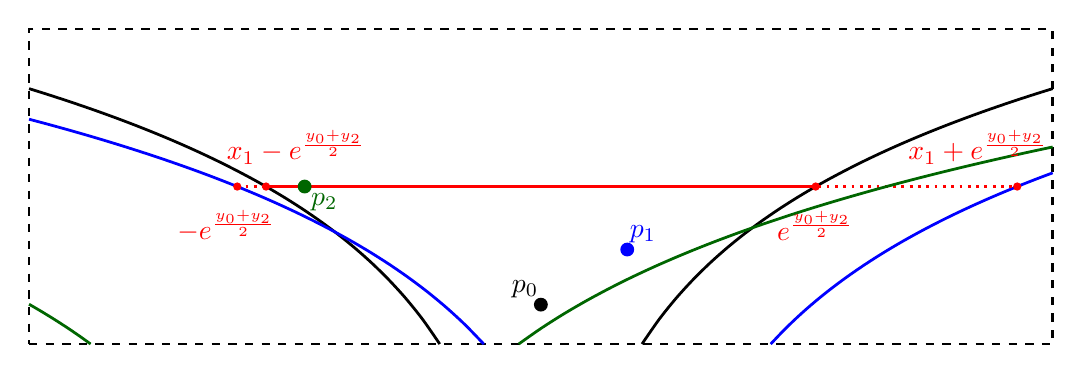
\begin{tikzpicture}
	%Define the coordinates 
	%p = (\u,\v) and p^\prime = (\uu, \vv)
	%Box \Rcal_n has width 2\r and height \t
	\pgfmathsetmacro{\u}{0} %0
	\pgfmathsetmacro{\v}{0.5} %1
	\pgfmathsetmacro{\vv}{1.2} %0.8
	\pgfmathsetmacro{\vvv}{2} %0.8
	\pgfmathsetmacro{\uuu}{-3} %1.4	
	\pgfmathsetmacro{\r}{6.5}
	\pgfmathsetmacro{\t}{4}
	
	\pgfmathsetmacro{\ubound}{exp((\vv+\vvv)/2)-exp((\v+\vvv)/2)}
	
	\pgfmathsetmacro{\uu}{3*\ubound/4}
	
	\pgfmathsetmacro{\leftintvandvvv}{-exp((\v + \vvv)/2)}
	\pgfmathsetmacro{\rightintvandvvv}{exp((\v + \vvv)/2)}
	\pgfmathsetmacro{\leftintvvandvvv}{\uu-exp((\vv + \vvv)/2)}
	\pgfmathsetmacro{\rightintvvandvvv}{\uu+exp((\vv + \vvv)/2)}
		
	%The box \Rcal_n
	\draw[line width=1pt,dashed] (-\r,0) -- (\r,0) -- (\r,\t) -- (-\r,\t) -- (-\r,0);

	%Dram all three nodes
    \draw node[fill, circle, inner sep=0pt, minimum size=5pt] (p1) at (\u,\v) {};
    \path (p1)+(-0.2,0.2) node {$p_0$};
    \draw node[fill,blue, circle, inner sep=0pt, minimum size=5pt] (p2) at (\uu,\vv) {};
    \path (p2)+(0.2,0.2) node {\color{blue}$p_1$};	
	
	%Boundaries p_0 = (\u,\v)
	
	%Right boundary
	\pgfmathsetmacro{\rightbounduv}{\u+exp((\v)/2)}
	\draw[domain=\rightbounduv:\r,smooth,variable=\x,black,line width=1pt] plot (\x, {2*ln(\x)-\v});
    %Left boundary
    \pgfmathsetmacro{\leftbounduv}{\u-exp((\v)/2)}
    \draw[domain=\leftbounduv:-\r,smooth,variable=\x,black,line width=1pt] plot (\x, {2*ln(-\x)-\v});
    
    %Boundaries p_1 = (\uu,\vv)
    
    %Right boundary
    \pgfmathsetmacro{\rightbounduuvv}{\uu+exp((\vv)/2)}
    \draw[domain=\rightbounduuvv:\r,smooth,variable=\x,blue,line width=1pt] plot (\x, {2*ln(\x-\uu)-\vv});
%    %Shifted right boundary
%    \pgfmathsetmacro{\shiftrightbounduuvv}{\uu+exp((\vv + \t)/2)-2*\r}
%    \draw[domain=\shiftrightbounduuvv:-\r,smooth,variable=\x,blue,line width=1pt] plot (\x, {2*ln(\x+(2*\r-\uu))-\vv});
    %Left boundary 
    \pgfmathsetmacro{\leftbounduuvv}{\uu-exp((\vv)/2)}
    \draw[domain=\leftbounduuvv:-\r,smooth,variable=\x,blue,line width=1pt] plot (\x, {2*ln(\uu-\x)-\vv});
%    %Shifted left boundary
%    \pgfmathsetmacro{\shiftleftbounduuvv}{\uu-exp((\vv + \t)/2)+2*\r}
%    \draw[domain=\shiftleftbounduuvv:\r,smooth,variable=\x,blue,line width=1pt] plot (\x, {2*ln(2*\r + \uu-\x)-\vv});
   


	\draw [red,dotted,line width=1pt] (\leftintvandvvv,\vvv) -- (\rightintvandvvv,\vvv);
	
	\draw [red,dotted,line width=1pt] (\leftintvvandvvv,\vvv) -- (\rightintvvandvvv,\vvv);

	\draw [red,line width=1pt] (\leftintvandvvv,\vvv) -- (\rightintvandvvv,\vvv);

    \draw node[fill,black!60!green, circle, inner sep=0pt, minimum size=5pt] (p2) at (\uuu,\vvv) {};
    \path (p2)+(0.25,-0.2) node {\color{black!60!green}$p_2$};
    
	%Boundaries p_2 = (\uuu,\vvv)
	
	%Right boundary
	\pgfmathsetmacro{\rightbounduuuvvv}{\uuu+exp((\vvv)/2)}
	\draw[domain=\rightbounduuuvvv:\r,smooth,variable=\x,black!60!green,line width=1pt] plot (\x, {2*ln(\x-\uuu)-\vvv});
    %Left boundary
    \pgfmathsetmacro{\leftbounduuuvvv}{\uuu-exp((\vvv)/2)}
    \draw[domain=\leftbounduuuvvv:-\r,smooth,variable=\x,black!60!green,line width=1pt] plot (\x, {2*ln(\uuu-\x)-\vvv});

	\draw node[fill,red, circle, inner sep=0pt, minimum size=3pt] at (\leftintvandvvv,\vvv) {};
	\path (\leftintvandvvv,\vvv)+(-0.5,-0.5) node[red] {$-e^{\frac{y_0 + y_2}{2}}$};
	\draw node[fill,red, circle, inner sep=0pt, minimum size=3pt] at (\rightintvandvvv,\vvv) {};
	\path (\rightintvandvvv,\vvv)+(0,-0.5) node[red] {$e^{\frac{y_0 + y_2}{2}}$};
	
	\draw node[fill,red, circle, inner sep=0pt, minimum size=3pt] at (\leftintvvandvvv,\vvv) {};
	\path (\leftintvvandvvv,\vvv)+(0.75,0.5) node[red] {$x_1 - e^{\frac{y_0 + y_2}{2}}$};
	\draw node[fill,red, circle, inner sep=0pt, minimum size=3pt] at (\rightintvvandvvv,\vvv) {};
	\path (\rightintvvandvvv,\vvv)+(-0.5,0.5) node[red] {$x_1 + e^{\frac{y_0 + y_2}{2}}$};

\end{tikzpicture}\\
\vspace{0.5cm}
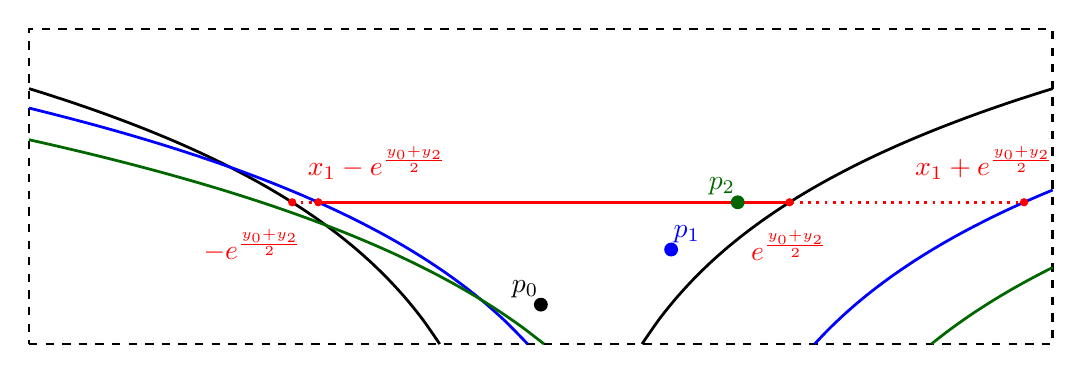
\begin{tikzpicture}
	%Define the coordinates 
	%p = (\u,\v) and p^\prime = (\uu, \vv)
	%Box \Rcal_n has width 2\r and height \t
	\pgfmathsetmacro{\u}{0} %0
	\pgfmathsetmacro{\v}{0.5} %1
	\pgfmathsetmacro{\vv}{1.2} %0.8
	\pgfmathsetmacro{\vvv}{1.8} %0.8
	\pgfmathsetmacro{\uuu}{2.5} %1.4	
	\pgfmathsetmacro{\r}{6.5}
	\pgfmathsetmacro{\t}{4}
	
	\pgfmathsetmacro{\ubound}{exp((\vv+\vvv)/2)-exp((\v+\vvv)/2)}
	
	\pgfmathsetmacro{\uu}{5*\ubound/4}
	
	\pgfmathsetmacro{\leftintvandvvv}{-exp((\v + \vvv)/2)}
	\pgfmathsetmacro{\rightintvandvvv}{exp((\v + \vvv)/2)}
	\pgfmathsetmacro{\leftintvvandvvv}{\uu-exp((\vv + \vvv)/2)}
	\pgfmathsetmacro{\rightintvvandvvv}{\uu+exp((\vv + \vvv)/2)}
		
	%The box \Rcal_n
	\draw[line width=1pt,dashed] (-\r,0) -- (\r,0) -- (\r,\t) -- (-\r,\t) -- (-\r,0);

	%Dram all three nodes
    \draw node[fill, circle, inner sep=0pt, minimum size=5pt] (p1) at (\u,\v) {};
    \path (p1)+(-0.2,0.2) node {$p_0$};
    \draw node[fill,blue, circle, inner sep=0pt, minimum size=5pt] (p2) at (\uu,\vv) {};
    \path (p2)+(0.2,0.2) node {\color{blue}$p_1$};	
	
	%Boundaries p_0 = (\u,\v)
	
	%Right boundary
	\pgfmathsetmacro{\rightbounduv}{\u+exp((\v)/2)}
	\draw[domain=\rightbounduv:\r,smooth,variable=\x,black,line width=1pt] plot (\x, {2*ln(\x)-\v});
    %Left boundary
    \pgfmathsetmacro{\leftbounduv}{\u-exp((\v)/2)}
    \draw[domain=\leftbounduv:-\r,smooth,variable=\x,black,line width=1pt] plot (\x, {2*ln(-\x)-\v});
    
    %Boundaries p_1 = (\uu,\vv)
    
    %Right boundary
    \pgfmathsetmacro{\rightbounduuvv}{\uu+exp((\vv)/2)}
    \draw[domain=\rightbounduuvv:\r,smooth,variable=\x,blue,line width=1pt] plot (\x, {2*ln(\x-\uu)-\vv});
    %Left boundary 
    \pgfmathsetmacro{\leftbounduuvv}{\uu-exp((\vv)/2)}
    \draw[domain=\leftbounduuvv:-\r,smooth,variable=\x,blue,line width=1pt] plot (\x, {2*ln(\uu-\x)-\vv});


	\draw [red,dotted,line width=1pt] (\leftintvandvvv,\vvv) -- (\rightintvandvvv,\vvv);
	
	\draw [red,dotted,line width=1pt] (\leftintvvandvvv,\vvv) -- (\rightintvvandvvv,\vvv);

	\draw [red,line width=1pt] (\leftintvvandvvv,\vvv) -- (\rightintvandvvv,\vvv);
	


    \draw node[fill,black!60!green, circle, inner sep=0pt, minimum size=5pt] (p2) at (\uuu,\vvv) {};
    \path (p2)+(-0.2,0.2) node {\color{black!60!green}$p_2$};
    
	%Boundaries p_2 = (\uuu,\vvv)
	
	%Right boundary
	\pgfmathsetmacro{\rightbounduuuvvv}{\uuu+exp((\vvv)/2)}
	\draw[domain=\rightbounduuuvvv:\r,smooth,variable=\x,black!60!green,line width=1pt] plot (\x, {2*ln(\x-\uuu)-\vvv});
    %Left boundary
    \pgfmathsetmacro{\leftbounduuuvvv}{\uuu-exp((\vvv)/2)}
    \draw[domain=\leftbounduuuvvv:-\r,smooth,variable=\x,black!60!green,line width=1pt] plot (\x, {2*ln(\uuu-\x)-\vvv});

	\draw node[fill,red, circle, inner sep=0pt, minimum size=3pt] at (\leftintvandvvv,\vvv) {};
	\path (\leftintvandvvv,\vvv)+(-0.5,-0.55) node[red] {$-e^{\frac{y_0 + y_2}{2}}$};
	\draw node[fill,red, circle, inner sep=0pt, minimum size=3pt] at (\rightintvandvvv,\vvv) {};
	\path (\rightintvandvvv,\vvv)+(0,-0.55) node[red] {$e^{\frac{y_0 + y_2}{2}}$};
	
	\draw node[fill,red, circle, inner sep=0pt, minimum size=3pt] at (\leftintvvandvvv,\vvv) {};
	\path (\leftintvvandvvv,\vvv)+(0.75,0.5) node[red] {$x_1 - e^{\frac{y_0 + y_2}{2}}$};
	\draw node[fill,red, circle, inner sep=0pt, minimum size=3pt] at (\rightintvvandvvv,\vvv) {};
	\path (\rightintvvandvvv,\vvv)+(-0.5,0.5) node[red] {$x_1 + e^{\frac{y_0 + y_2}{2}}$};

\end{tikzpicture}
\caption{Situation for the intersections of the connection intervals considered in Lemma~\ref{lem:ordered}, with $y_0 < y_1 <y_2$ fixed and for different cases of $0 \le x_1 \le e^{(y_0 + y_1)/2}$. The top figure shows the case where $0 \le x_1 \le e^{(y_1 + y_2)/2} - e^{(y_0 + y_2)/2}$, while the bottom one shows the case $x_1 > e^{(y_1 + y_2)/2} - e^{(y_0 + y_2)/2}$. The solid red line indicates the range for $x_2$ such that the points $p_0$, $p_1$ and $p_2$ form a triangle. The boundaries of their neighborhoods are shown in, respectively, black, blue and green.}
\label{fig:triangle_prob_lemma}
\end{figure}

\begin{proof}
Note that $P(y_0,y_1,y_2)$ is the probability that $x_2$ falls into the interval $[x_1-e^{(y_1+y_2)/2},x_1+e^{(y_1+y_2)/2}]$, as well as into the interval $[-e^{(y_0+y_2)/2},e^{(y_0+y_2)/2}]$. By symmetry considerations, we can take $x_1$ uniformly at random from $[0,e^{y_0/2+y_1/2}]$ as opposed to $[-e^{y_0/2+y_1/2}, e^{y_0/2+y_1/2}]$. Figure~\ref{fig:triangle_prob_lemma} shows the intersection of the intervals (red line) for two different cases for $x_1 \le e^{(y_0 + y_1)/2}$. 

Since $y_0 < y_1 < y_2$ we have that $e^{(y_1+y_2)/2} > e^{(y_0+y_2)/2}$ and so, when $x_1 \geq 0$, the ``right half'' of the 
interval $[-e^{(y_0+y_2)/2}, e^{(y_0+y_2)/2}]$ is always covered by the interval $[x_1-e^{(y_1+y_2)/2}, x_1+e^{(y_1+y_2)/2}]$.
If $e^{(y_1+y_2)/2} - e^{(y_0+y_1)/2} \geq e^{(y_0+y_2)/2}$ then the ``left half'' is always covered as well.
In other words:
\[
	e^{(y_1+y_2)/2} - e^{(y_0+y_1)/2} \geq e^{(y_0+y_2)/2} \Rightarrow P(y_0,y_1,y_2) = 1.
\]

Now consider the case where $e^{(y_1+y_2)/2} - e^{(y_0+y_1)/2} < e^{(y_0+y_2)/2}$. 
Then, if $x_1 \in [0, e^{(y_1+y_2)/2} - e^{(y_0+y_2)/2}]$ the whole interval $[-e^{(y_0+y_2)/2}, e^{(y_0+y_2)/2}]$ is still covered 
so that $p_0, p_1$ and $p_2$ form a triangle. If, on the other hand $e^{(y_1+y_2)/2} - e^{(y_0+y_2)/2} < x_1 \leq e^{(y_0+y_1)/2}$ then
the probability that $|x_2-x_1| \leq e^{(y_1+y_2)/2}$ equals
\[ 
	1 - \frac{x_1 - (e^{(y_1+y_2)/2} - e^{(y_0+y_2)/2)}) }{ 2e^{(y_0+y_2)/2} }. 
\]

Hence, when $e^{(y_1+y_2)/2} - e^{(y_0+y_1)/2} < e^{(y_0+y_2)/2}$ we have
\begin{align*}
	P(y_0,y_1,y_2) &= \frac{e^{(y_1+y_2)/2} - e^{(y_0+y_2)/2} }{ e^{(y_0+y_1)/2} }  \\
	&\hspace{10pt}+ \int_{ e^{(y_1+y_2)/2} - e^{(y_0+y_2)/2} }^{ e^{(y_0+y_1)/2} } 
	    \left(1 - \frac{x_1 - (e^{(y_1+y_2)/2} - e^{(y_0+y_2)/2)}) }{ 2e^{(y_0+y_2)/2} }\right)
	    \cdot \frac{1}{e^{(y_0+y_1)/2}} \dd x_1 \\
	&= 1 - \frac{1}{2e^{y_0+y_1/2+y_2/2} } \int_0^{ e^{(y_0+y_1)/2}+e^{(y_0+y_2)/2}-e^{(y_1+y_2)/2} } x_1 \dd x_1 \\
	&= 1 - \frac{ \left( e^{(y_0+y_1)/2}+e^{(y_0+y_2)/2}-e^{(y_1+y_2)/2} \right)^2 }{ 4 e^{y_0+y_1/2+y_2/2} },
\end{align*}

At this point it is convenient to rewrite everything in terms of $z_i := e^{-y_i/2}$.
Note that $y_0 < y_1 < y_2$ if and only if $z_0 > z_1 > z_2$ while the condition $e^{(y_1+y_2)/2} - e^{(y_0+y_1)/2} < e^{(y_0+y_2)/2}$ becomes
\[ e^{(y_1+y_2)/2} - e^{(y_0+y_1)/2} < e^{(y_0+y_2)/2} \Leftrightarrow 
z_1^{-1} z_2^{-1} < z_0^{-1} z_1^{-1} + z_0^{-1}z_2^{-1} 
\Leftrightarrow
z_0 < z_1+z_2. 
\]

We now conclude that
\[
	P(y_0(z_0), y_1(z_1), y_2(z_2)) = 1 \quad \text{if} \quad z_0 > z_1 > z_2 \text{ and } z_0 \geq z_1 + z_2
\]
while for $z_0 > z_1 > z_2$ and $z_0 < z_1 + z_2$
\begin{align*}
	P(y_0(z_0), y_1(z_1), y_2(z_2)) 
	&= 1 - \frac{z_0^2z_1z_2}{4} \cdot \left( z_0^{-1}z_1^{-1}+z_0^{-1}z_2^{-1}-z_1^{-1}z_2^{-1} \right)^2 \\
%	&= 1 - \frac{z_0^2z_1z_2}{4} \cdot \left( z_0^{-2}z_1^{-2} + z_0^{-2}z_2^{-2} + z_1^{-2}z_2^{-2}
%		+ 2z_0^{-2}z_1^{-1}z_2^{-1} - 2 z_0^{-1}z_1^{-2}z_2^{-1} - 2z_0^{-1}z_1^{-1}z_2^{-2} \right) \\
	&= 1 - \frac{1}{4} \left( z_1^{-1}z_2 + z_1z_2^{-1} + z_0^2z_1^{-1}z_2^{-1} + 2 - 2z_0z_1^{-1}-2z_0z_2^{-1}\right),
\end{align*}
which finishes the proof.
\end{proof}

The previous lemma covers the case when $y_0<y_1<y_2$. We now leverage it to take care of the other cases as well. 

\begin{proof}[Proof of Lemma~\ref{lem:triangle_prob_y_coordinates}]
Let $y_i >0$ and $z_i = e^{-y_i/2}$, $i=0,1,2$. Lemma~\ref{lem:ordered} gives the expression for $P(y_0(z_0),y_1(z_1),y_2(z_2))$ in the case $y_0<y_1<y_2$, or equivalently $z_0>z_1>z_2$, i.e. the first two lines in the claim of Lemma~\ref{lem:triangle_prob_y_coordinates}. To analyze the other cases we shall express $P(y_1,y_0,y_2)$ and $P(y_1,y_2,y_0)$ in terms of $P(y_0,y_1,y_2)$ and $z_i$. For this we note that we can view $P(y_0,y_1,y_2)$ as a 2-fold integral of the indicator function
\[ 
	h(x_0, x_1, x_2) := \ind{ |x_0 - x_1| < e^{(y_0+y_1)/2}, |x_0 - x_2| < e^{(y_0+y_2)/2}, |x_1-x_2| < e^{(y_1+y_2)/2}}, 
\]
where $x_0$ was set to zero, without loss of generality, and the other two $x_i$ are uniform random variables on $[-e^{(y_0+y_i)/2}, e^{(y_0+y_i)/2}]$. When we consider the probability $P(y_1,y_0,y_2)$, this is the 2-fold integral of $h(x_0,0,x_2)$ so that
\begin{align*}
	P(y_1,y_0,y_2) &= \frac{1}{2e^{(y_1+y_0)/2}} \cdot \frac{1}{2e^{(y_1+y_2)/2}} 
		\iint_{\R} h(x_0,0,x_2) \dd x_0 \dd x_2\\
	&= \frac{e^{y_0/2}}{e^{y_1/2}} \frac{1}{2e^{(y_0+y_1)/2}} \frac{1}{2e^{(y_0+y_2)/2}} 
		\iint_{\R} h(0,x_1,x_2) \dd x_1 \dd x_2\\
	&= \frac{e^{y_0/2}}{e^{y_1/2}} P(y_0,y_1,y_2) = \frac{z_1}{z_0}  P(y_0,y_1,y_2).
\end{align*}
Finally we note that $h(x_0,0,x_2) = h(x_2,0,x_0)$ from which we conclude that
\begin{equation}\label{eq:symmetry_relation_triangle_prob}
	P(y_0, y_1, y_2) = \left(z_0/z_1\right) P(y_1,y_0,y_2) = \left(z_0/z_1\right) P(y_1,y_2,y_0).
\end{equation}

To complete the proof for the other cases we note that since $P(y_0,y_1,y_2)$ is symmetric in $y_1$ and $y_2$, we can assume, without loss of generality, that $y_1 < y_2$. Then, there are two more orderings of $y_0, y_1, y_2$, namely $y_1< y_0< y_2$ and $y_1<y_2<y_0$, which can be summarized as $y_1 < \min (y_0,y_2)$, or equivalently $z_1 > \max(z_0,z_2)$. For $y_1 < y_0 < y_2$ and $y_1 < y_2<y_0$ we can apply Lemma~\ref{lem:ordered} to obtain $P(y_1,y_0,y_2) = P(y_1,y_2,y_0)$ which happen to agree due to the symmetry in the last two arguments of the expression found in Lemma~\ref{lem:ordered}. The expression for $P(y_0,y_1,y_2)$ then follows from~\eqref{eq:symmetry_relation_triangle_prob}.
\end{proof}

%


\subsubsection{Integrating over $y_1, y_2$}


Now that we have established the expression for $P(y_0,y_1,y_2)$ we can proceed to compute $P(y_0)$ by integrating over $y_1, y_2$.
We however start with the following observation.

\begin{lemma}\label{lem:continuity_Delta_function}
The function $\alpha \mapsto P_\alpha(y_0)$ is continuous for all $\alpha > \frac{1}{2}$.
\end{lemma}

\begin{proof}
This follows from the theorem of dominated convergence:
Let $\alpha > \frac{1}{2}$ and $(\alpha_n)_{n\in \mathbb{N}}$ a sequence of real numbers converging to $\alpha$, so we can 
assume $|\alpha_n - \alpha| < \epsilon := \frac{\alpha-1/2}{2}$. 
This means that $-\epsilon < \alpha_n - \alpha < \epsilon$, i.e. $\frac{\alpha-1/2}{2} < \alpha_n - 1/2 < \frac{3\alpha-3/2}{2}$. Define 

$$f_n(y_1,y_2) = P(y_0,y_1,y_2) (\alpha_n - 1/2)^2 e^{-(\alpha_n-1/2)(y_1+y_2)}.$$ 

As the function $x \mapsto x^2$ is increasing in $x$ for $x>0$ and the function $x \mapsto e^{-(y_1+y_2)x}$ is decreasing 
in $x$ and $P(y_0,y_1,y_2) \in [0,1]$, it holds that 

$$|f_n(y_1,y_2)| \leq \left(\frac{3\alpha-3/2}{2}\right)^2e^{-(y_1+y_2)\frac{\alpha-1/2}{2}}$$

which is integrable over $\R_{\geq 0} \times \R_{\geq 0}$ (with integral equalling $(6\alpha-3)^2/(2\alpha-1)^2$). 
Application of the theorem of dominated convergence yields that 
$P_{\alpha_n}(y_0) \rightarrow P_\alpha(y_0)$ which gives the claim as the 
sequence $(\alpha_n)_n$ was arbitrary.
\end{proof}

Due to this lemma we can first assume $\alpha \notin \{ \frac{3}{4},1 \}$, compute $P(y_0)$ and then obtain the values of $P(y_0)$ at 
the remaining two points by taking the corresponding limit in $\alpha$. 
This strategy is executed below. 
It involves the computation of several integrals which are involved and will take up a few pages. 
The proof is structured using headers, to aid the reader. 


%\begin{proof}[Proof of Proposition~\ref{prop:full_expression_delta_P}]\hfill


%\paragraph{When $\bm{\alpha \notin \{3/4,1\}}$}

Note that when writing $P(y_0)$ as an integral, see equation~\eqref{eq:delta_P}, by symmetry in the integration 
variables $y_1$ and $y_2$, we can assume that $y_1<y_2$ in which case either $y_0$ or $y_1$ is the smallest height. 
This gives half the value of $P(y_0)$ and hence
\[ 
	P(y_0) = 2(I_1(y_0) +I_2(y_0)), 
\] 
where $I_1$ and $I_2$ are given by:
\begin{align*}
	I_1(y_0) &:= \int_{0<y_0<y_1<y_2} P(y_0,y_1,y_2) \cdot (\alpha-1/2)^2 e^{-(\alpha-1/2)(y_1+y_2)}  \dd y_2 \dd y_1 \\ 
	I_2(y_0) &:= \int_{0<y_1<y_0,y_2} P(y_0,y_1,y_2) \cdot (\alpha-1/2)^2 e^{-(\alpha-1/2)(y_1+y_2)} \dd y_2 \dd y_1 \\ 
\end{align*}

We proceed with computing each of these two integrals, each of which is split in two parts. 
The final expressions of those four integrals can be found 
in~\eqref{eq:Delta_P_computation_I11}, \eqref{eq:Delta_P_computation_I12}, \eqref{eq:Delta_P_computation_I21} 
and~\eqref{eq:Delta_P_computation_I22}.

\paragraph{Computing $\bm{I_1(y_0)}$}

Applying the change of variables $z_i := e^{-y_i/2}$, $i=1,2$, and Lemma~\ref{lem:triangle_prob_y_coordinates} gives %${\dd}y_i = -\frac{2{\dd}z_i}{z_i}$ and therefore
\begin{align*}
	I_1(y_0) &=	4 (\alpha-1/2)^2 \cdot \int_{z_0>z_1>z_2>0} P(y_0,y_1(z),y_2(z)) z_1^{2\alpha-2} z_2^{2\alpha-2} 
		{\dd}z_2{\dd}z_1 \\
	&= 4 (\alpha-1/2)^2 \cdot \left( \int_{z_0>z_1>z_2>0} 1 \cdot z_1^{2\alpha-2} z_2^{2\alpha-2} 
		{\dd}z_2{\dd}z_1 \right. \\
	&\hspace{10pt} \left. - \int_{{z_0>z_1>z_2>0,}\atop{z_0 < z_1+z_2}} G(z_0,z_1,z_2) \cdot z_1^{2\alpha-2} z_2^{2\alpha-2} 
		{\dd}z_2{\dd}z_1 \right) \\
	&=: 4 (\alpha-1/2)^2 ( I_{11}(y_0) - I_{12}(y_0)). 
\end{align*}

The integral $I_{11}(y_0)$ is easily obtained:
\begin{align*}
	I_{11}(y_0) &= \int_0^{z_0} \int_0^{z_1} z_1^{2\alpha-2} z_2^{2\alpha-2} {\dd}z_2{\dd}z_1
		= \int_0^{z_0} z_1^{2\alpha-2} \left[ \frac{z_2^{2\alpha-1}}{2\alpha-1} \right]_0^{z_1} {\dd}z_1\\
	&= \frac{1}{2\alpha-1} \cdot \int_0^{z_0} z_1^{4\alpha-3} {\dd}z_1
		= \frac{1}{2(2\alpha-1)^2} \cdot z_0^{4\alpha-2}. \numberthis \label{eq:Delta_P_computation_I11}
\end{align*}

To deal with $I_{12}$ we note that $G(z_0,z_1,z_2)$ is a linear combination of monomials of the form $z_0^az_1^bz_2^c$ with 
$a,b,c \in \{-1,0,1,2\}$ and $a+b+c=0$. Let us consider the integral $J_{(a,b,c)}(z_0)$ defined by 

\begin{equation}\label{eq:def_Delta_P_computation_int_J_1}
	J_{a,b,c}(z_0) := z_0^a \int_{{z_0>z_1>z_2>0,}\atop{z_0 < z_1+z_2}} z_1^{b+2\alpha-2} z_2^{c+2\alpha-2} {\dd}z_2{\dd}z_1.
\end{equation}
and note that
\begin{equation}\label{eq:Delta_P_computation_I12_with_J}
	I_{1,2}(y_0) = \frac{1}{4} (J_{0,-1,1}(z_0)+J_{0,1,-1}(z_0)+J_{2,-1,-1}(z_0)+2J_{0,0,0}(z_0)-2J_{1,-1,0}(z_0)-2J_{1,0,-1}(z_0)).
\end{equation}

Next we compute $J_{a,b,c}(z_0)$.
\begin{align*}
	J_{a,b,c}(z_0) 
	&= z_0^a \int_{z_0/2}^{z_0}\int_{z_0-z_1}^{z_1} z_1^{b+2\alpha-2} z_2^{c+2\alpha-2} {\dd}z_2{\dd}z_1
		= z_0^a \int_{z_0/2}^{z_0} z_1^{b+2\alpha-2} \left[ \frac{ z_2^{c+2\alpha-1} }{ c+2\alpha-1 } \right]_{z_0-z_1}^{z_1} \dd z_1\\
	&= \frac{z_0^a}{c+2\alpha-1} \cdot \left( \int_{z_0/2}^{z_0} z_1^{b+c+4\alpha-3} \dd z_1
	   - \int_{z_0/2}^{z_0} z_1^{b+2\alpha-2} (z_0-z_1)^{c+2\alpha-1} {\dd}z_1 \right) \\
	&= \frac{z_0^{a+b+c+4\alpha-2}(1-(1/2)^{b+c+4\alpha-2})}{(c+2\alpha-1)(b+c+4\alpha-2)} \\
	&\hspace{10pt}- \frac{z_0^{a+b+c+4\alpha-3}}{c+2\alpha-1} \int_{z_0/2}^{z_0}  \left(z_1/z_0\right)^{b+2\alpha-2} 
	    \left(1-(z_1/z_0)\right)^{c+2\alpha-1} \dd z_1\\
	&= \frac{z_0^{4\alpha-2}(1-(1/2)^{b+c+4\alpha-2})}{(c+2\alpha-1)(b+c+4\alpha-2)} 
		- \frac{z_0^{4\alpha-2}}{c+2\alpha-1}
	   \int_{1/2}^1  u^{b+2\alpha-2}(1-u)^{c+2\alpha-1} \dd u \\
	&= \frac{z_0^{4\alpha-2}(1-(1/2)^{b+c+4\alpha-2})}{(c+2\alpha-1)(b+c+4\alpha-2)} 
		- \frac{z_0^{4\alpha-2}}{c+2\alpha-1} B^-(1/2;c+2\alpha, b+2\alpha-1),
\end{align*}
where we have used the substitution $u := z_1/z_0$ giving $z_0 {\dd} u = {\dd} z_1$ in the penultimate line and
$B^-$ denotes the (lower) incomplete beta function. Note that since $c \geq -1$, $-a \in \{0,-1,-2\}$ and by our assumption $\alpha \not \in \{\frac{3}{4},1\}$, the denominators that occur during the integration are all non-zero.

Plugging this back into~\eqref{eq:Delta_P_computation_I12_with_J} gives
\begin{align*}
	I_{1,2}(y_0)
	&= \frac{z_0^{4\alpha-2}(1-(1/2)^{4\alpha-2})}{32\alpha(\alpha-1/2)} 
   		- \frac{z_0^{4\alpha-2}}{8\alpha} B^-(1/2;1+2\alpha, 2\alpha-2)\\
	&\hspace{10pt}+ \frac{z_0^{4\alpha-2}(1-(1/2)^{4\alpha-2})}{32(\alpha-1)(\alpha-1/2)} 
   		-  \frac{z_0^{4\alpha-2}}{4(2\alpha-2)} B^-(1/2;2\alpha-1,2\alpha)\\
	&\hspace{10pt}+ \frac{z_0^{4\alpha-2}(1-(1/2)^{4\alpha-4})}{32(\alpha-1)^2} 
   		- \frac{z_0^{4\alpha-2}}{4(2\alpha-2)} B^-(1/2;-1+2\alpha, 2\alpha-2)\\
	&\hspace{10pt}+ \frac{z_0^{4\alpha-2}(1-(1/2)^{4\alpha-2})}{16(\alpha-1/2)^2} 
   		- \frac{z_0^{4\alpha-2}}{2(2\alpha-1)} B^-(1/2;2\alpha,2\alpha-1)\\
	&\hspace{10pt}- \frac{z_0^{4\alpha-2}(1-(1/2)^{4\alpha-3})}{16(\alpha-1/2)(\alpha-3/4)} 
   		+ \frac{z_0^{4\alpha-2}}{2(2\alpha-1)} B^-(1/2;2\alpha, 2\alpha-2)\\
	&\hspace{10pt}- \frac{z_0^{4\alpha-2}(1-(1/2)^{4\alpha-3})}{16(\alpha-1)(\alpha-3/4)} 
   		+ \frac{z_0^{4\alpha-2}}{2(2\alpha-2)} B^-(1/2;-1+2\alpha, 2\alpha-1) \\
	&=\frac{\left(\frac{3}{64}- \frac{3}{16} 2^{-4\alpha}+ 
   		\alpha (-\frac{41}{128} + \frac{13}{16}  2^{-4\alpha}) 
   		+ \alpha^2 (\frac{5}{8} - \frac{3}{4} 2^{-4\alpha}) - \frac{15}{32}\alpha^3 +\frac{1}{8} a^4\right) 
   		z_0^{4 \alpha-2} }{4(\alpha-1/2)^2 (\alpha-1)^2 (\alpha-3/4) \alpha} \\
	&\hspace{10pt}+ \frac{z_0^{4\alpha-2}}{8 (\alpha-1) \alpha (2\alpha-1)}(4 (\alpha-1) \alpha 
		(B^-(1/2; 2\alpha, 2\alpha-2) - B^-(1/2;2 \alpha,2\alpha-1) ) \\
    &\hspace{10pt}- (2 \alpha-1)\alpha ( B^-(1/2; 2\alpha-1, 2\alpha-2) + 
    	B^-(1/2; 2\alpha-1, 2\alpha) - 
    	2 B^-(1/2;2\alpha -1, 2\alpha-1) ) \\
    &\hspace{10pt}- (2\alpha-1)(\alpha-1) B^-(1/2; 1 + 2\alpha, 2\alpha-2)) \\
	&=\frac{\left(\frac{3}{64}- \frac{3}{16} 2^{-4\alpha} 
		+ \alpha (-\frac{41}{128} + \frac{13}{16}  2^{-4\alpha})  
		+ \alpha^2 (\frac{5}{8} - \frac{3}{4} 2^{-4\alpha}) - \frac{15}{32}\alpha^3 +\frac{1}{8} a^4\right) 
		z_0^{4 \alpha-2} }{4(\alpha-1/2)^2 (\alpha-1)^2 (\alpha-3/4) \alpha} \\
 	&\hspace{10pt}+ \frac{z_0^{4\alpha-2}}{8 (\alpha-1) \alpha (2\alpha-1)}(4 (\alpha-1) \alpha 
 		B^-(1/2; 2\alpha+1, 2\alpha-2) \\
  	&\hspace{10pt}- (2 \alpha-1)\alpha B^-(1/2;2\alpha+1,2\alpha-2) \\
    &\hspace{10pt}- (2\alpha-1)(\alpha-1) B^-(1/2; 2\alpha+1, 2\alpha-2)). \\
\end{align*}
For the last step we use the identities 
\begin{align}
	B^-(z;a,b)-B^-(z;a,b+1) &= B^-(z; a+1,b), \label{eq:Delta_P_computation_beta_id_1}\\
	B^-(z;a,b)+B^-(z;a,b+2)-2B^-(z;a,b+1) &= B^-(z;a+2,b). \label{eq:Delta_P_computation_beta_id_2}
\end{align}
to obtain
\begin{equation}
\begin{aligned}
	I_{1,2}(y_0) &=\frac{\left(\frac{3}{64}- \frac{3}{16} 2^{-4\alpha}
		+ \alpha (-\frac{41}{128} + \frac{13}{16}  2^{-4\alpha})
		+ \alpha^2 (\frac{5}{8} - \frac{3}{4} 2^{-4\alpha}) - \frac{15}{32}\alpha^3 +\frac{1}{8} a^4\right) 
		z_0^{4 \alpha-2} }{4(\alpha-1/2)^2 (\alpha-1)^2 (\alpha-3/4) \alpha} \\
 	&\hspace{10pt}- \frac{z_0^{4\alpha-2}B^-(1/2; 2\alpha+1, 2\alpha-2) }{8 (\alpha-1) \alpha (2\alpha-1)}	\label{eq:Delta_P_computation_I12}
\end{aligned}
\end{equation}


\paragraph{Computing $\bm{I_2(y_0)}$}

We will follow a similar strategy as for $I_1(y_0)$. First, using the change of variables $z_i := e^{-y_i/2}$, $i=1,2$,
we get
\begin{align*}
	I_2(y_0) &= 4 (\alpha-1/2)^2 \cdot \int_{1>z_1>z_2,z_0>0} P(y_0,y_1(z_1),y_2(z_2)) z_1^{2\alpha-2} z_2^{2\alpha-2} 
		{\dd}z_2{\dd}z_1 \\
	&= 4 (\alpha-1/2)^2 \cdot \left( \int_{1>z_1>z_0,z_2>0}  z_0 z_1^{2\alpha-3} z_2^{2\alpha-2} 
		{\dd}z_2{\dd}z_1 \right. \\
	&\hspace{10pt}\left. - \int_{{1>z_1>z_0,z_2>0}\atop{z_1 < z_0+z_2}} G(z_1,z_0,z_2) z_0 z_1^{2\alpha-3} 	
		z_2^{2\alpha-2} \dd z_2{\dd}z_1 \right) \\
	&=: 4 (\alpha-1/2)^2 (I_{21}(y_0) - I_{22}(y_0)). 
\end{align*}

We proceed with the easy integral:
\begin{align*}
	I_{21}(y_0) &= z_0 \int_{1>z_1>\max(z_2,z_0);z_0,z_2>0} z_1^{2\alpha-3} z_2^{2\alpha-2} {\dd}z_2{\dd}z_1   
		= z_0 \int_{z_0}^1 \int_{0}^{z_1} z_1^{2\alpha-3} z_2^{2\alpha-2} {\dd}z_2{\dd}z_1\\
	&= z_0 \int_{z_0}^1 \left[ \frac{z_2^{2\alpha-1}}{2\alpha-1}\right]_{0}^{z_1} z_1^{2\alpha-3} {\dd}z_1 
		= \frac{z_0}{2\alpha-1}  \int_{z_0}^1 z_1^{4\alpha-4} {\dd}z_1
		= \frac{z_0 - z_0^{4\alpha-2}}{(4\alpha-3)(2\alpha-1)}. \numberthis \label{eq:Delta_P_computation_I21}
\end{align*}
We note that the denominators above are non-zero as $\alpha > \frac{1}{2}$ and $\alpha \not =\frac{3}{4}$.

To deal with $I_{22}(y_0)$ we consider the integral function
\[
	J_{a,b,c}^\prime(z_0) := z_0^a \int_{{1>z_1>\max(z_0,z_2); z_0,z_2>0}\atop{z_1 < z_0+z_2}} z_1^{b+2\alpha-2} z_2^{c+2\alpha-2} {\dd}z_2{\dd}z_1
\]
and note that
\begin{equation}\label{eq:Delta_P_computation_I22_J}
\begin{aligned}
		I_{2,2}(y_0) &= \frac{1}{4}\left(J_{0,-1,1}^\prime(z_0) + J_{2,-1,-1}^\prime(z_0)
		+ J_{0,1,-1}^\prime(z_0)\right) \\
		&\hspace{10pt}+ \frac{1}{2}\left( J_{1,-1,0}^\prime(z_0) - J_{0,0,0}^\prime(z_0) - J_{1,0,-1}^\prime(z_0)\right).
\end{aligned}
\end{equation}

We now compute $J_{a,b,c}^\prime(z_0)$
\begin{align*}
	J_{a,b,c}^\prime(z_0) 
	&= z_0^a \int_{z_0}^1 \int_{z_1-z_0}^{z_1}  z_1^{b+2\alpha-2} z_2^{c+2\alpha-2} {\dd} z_2 {\dd} z_1  \\
 	&= z_0^a \int_{z_0}^1 \frac{1}{c+2\alpha-1}  z_1^{b+2\alpha-2}( z_1^{c+2\alpha-1}-(z_1-z_0)^{c+2\alpha-1})  {\dd} z_1  \\
 	&=z_0^a \int_{z_0}^1 \frac{1}{c+2\alpha-1} z_1^{b+c+4\alpha-3} {\dd } z_1 -z_0^{a} \int_{z_0}^1 	
 		\frac{1}{c+2\alpha-1}z_1^{b+2\alpha-2}(z_1-z_0)^{c+2\alpha-1}  {\dd} z_1  \\
 	&= z_0^a  \frac{1}{(c+2\alpha-1)(b+c+4\alpha-2)}(1-z_0^{b+c+4\alpha-2}) \\
 	&\hspace{10pt}- \frac{z_0^a}{c+2\alpha-1}z_0^{b+c+4\alpha-2}B^-(1-z_0;c+2\alpha,-b-c-4\alpha+2) \\
	&= \frac{z_0^a -z_0^{4\alpha-2}}{(c+2\alpha-1)(b+c+4\alpha-2)}  
		- \frac{z_0^{4\alpha -2}B^-(1-z_0;c+2\alpha,-b-c-4\alpha+2)}{c+2\alpha-1}.  
\end{align*}
Here we used that for $x  \in \R,y>-1$ (note that as $c\geq -1$, it holds that $c+2\alpha-1 >-1$):
\begin{align*}
 \int_{z_0}^{1} z_1^x (z_1-z_0)^y {\dd} z_1 
 &= \int_0^{1-z_0} (s+z_0)^x s^y {\dd} s \\
 &= z_0^{x+y} \int_0^{1-z_0} \left( (s/z_0) + 1 \right)^x (s/z_0)^y {\dd} s \\
 &= z_0^{x+y+1} \int_{0}^{1/z_0 -1 } (t+1)^x t^y {\dd} t \\
 &= z_0^{x+y+1} \int_0^{1-z_0} u^y (1-u)^{-(x+y+2)} {\dd} u \\
 &= z_0^{x+y+1} B^-(1-z_0; y+1,-x-y-1 ).
\end{align*}
As $c \geq -1$ and $-a \in \{0,-1,-2\}$ and by our assumption $\alpha \not \in \{\frac{3}{4}\}$, the denominators 
that occur during the computations above are non-zero. 

Plugging the expression for $J_{a,b,c}^\prime(z_0)$ back into~\eqref{eq:Delta_P_computation_I22_J} we get,
\begin{align*}
	I_{2,2}(y_0) 
	&= \frac{1 -z_0^{4\alpha-2}}{32\alpha(\alpha-1/2)} 
		-  \frac{z_0^{4\alpha -2}B^-(1-z_0;1+2\alpha,-4\alpha+2)}{8\alpha} \\
	&\hspace{10pt}+ \frac{z_0^2 -z_0^{4\alpha-2}}{32(\alpha-1)^2}  
		- \frac{z_0^{4\alpha -2}B^-(1-z_0;-1+2\alpha,-4\alpha+4)}{8(\alpha-1)} \\
	&\hspace{10pt}+ \frac{1 -z_0^{4\alpha-2}}{32(\alpha-1)(\alpha-1/2)}  
		- \frac{z_0^{4\alpha -2}B^-(1-z_0;-1+2\alpha,-4\alpha+2)}{8(\alpha-1)} \\
	&\hspace{10pt}+ \frac{z_0 -z_0^{4\alpha-2}}{16(\alpha-1/2)(\alpha-3/4)}  
		- \frac{z_0^{4\alpha -2}B^-(1-z_0;2\alpha,-4\alpha+3)}{4(\alpha-1/2)} \\
	&\hspace{10pt}- \frac{1 -z_0^{4\alpha-2}}{16(\alpha-1/2)^2}  
		+ \frac{z_0^{4\alpha -2}B^-(1-z_0;2\alpha,-4\alpha+2)}{4(\alpha-1/2)}\\
	&\hspace{10pt}-\frac{z_0 -z_0^{4\alpha-2}}{16(\alpha-1)(\alpha-3/4)} 
		+ \frac{z_0^{4\alpha -2}B^-(1-z_0;-1+2\alpha,-4\alpha+3)}{4(\alpha-1)}.
\end{align*}
Using some algebra and the identities~\eqref{eq:Delta_P_computation_beta_id_1} and~\eqref{eq:Delta_P_computation_beta_id_2}  
this can be reduced to
\begin{equation}\label{eq:Delta_P_computation_I22}
\begin{aligned}
	I_{2,2}(y_0)
	&=\frac{1}{64\alpha(\alpha-1/2)^2(\alpha-1)} -\frac{(1 - z_0)^{2\alpha}}{64\alpha(\alpha-1/2)^2 (\alpha-1)} 
		- \frac{z_0}{8(\alpha-1/2)(\alpha-1)(4\alpha-3)}\\ 
	&\hspace{10pt}+ \frac{z_0^2}{32(\alpha-1)^2} + \frac{(-6 + 25\alpha - 48\alpha^2 + 44\alpha^3 -16\alpha^4) 
   		z_0^{4\alpha-2}}{512\alpha(\alpha-1/2)^2(\alpha-1)^2(\alpha-3/4)} \\
	&\hspace{10pt}+ \frac{z_0^{4\alpha-2}B^-(1 - z_0; 2\alpha, 3 - 4\alpha)}{32(\alpha-1)(\alpha-1/2)^2}.
\end{aligned}
\end{equation}



\paragraph{Combining the results for $\bm{I_1(y_0)}$ and $\bm{I_2(y_0)}$}



Combining the results for $I_{11}(y_0), I_{12}(y_0), I_{21}(y_0)$ and $I_{22}(y_0)$ we get, after some algebra, an explicit expression 
for $P(y_0)$ as a linear combination of terms of the form $z_0^u$, $(1-z_0)^u$ and $z_0^u B^-(1-z_0;a,b)$: 
\begin{align*}
P(y_0)=& 2(I_1+I_2) = 8(\alpha- 1/2)^2(I_{1,1}-I_{1,2}+I_{2,1}-I_{2,2}) \\
=&8(\alpha-1/2)^2 \left(\frac{1}{2(2\alpha-1)^2 }z_0^{4\alpha -2} \right. \\ 
&\left.-\frac{\left(\frac{3}{64}- \frac{3}{16} 2^{-4\alpha}+ 
   \alpha (-\frac{41}{128} + \frac{13}{16}  2^{-4\alpha})  + 
   \alpha^2 (\frac{5}{8} - \frac{3}{4} 2^{-4\alpha}) - \frac{15}{32}\alpha^3 +\frac{1}{8} a^4   \right) z_0^{4 \alpha-2} }{4(\alpha-1/2)^2 (\alpha-1)^2 (\alpha-3/4) \alpha} \right. \\ 
&\left.+\frac{z_0^{4\alpha-2}B^-(1/2; 2\alpha+1, 2\alpha-2) }{8 (\alpha-1) \alpha (2\alpha-1)} +\frac{z_0 - z_0^{4\alpha -2}}{(4\alpha-3)(2\alpha-1)} \right.\\
&\left.-\frac{1}{64\alpha(\alpha-1/2)^2(\alpha-1)} +\frac{(1 - z_0)^{2\alpha}}{64\alpha(\alpha-1/2)^2 (\alpha-1)} +\frac{z_0}{8(\alpha-1/2)(\alpha-1)(4\alpha-3)} \right.\\
   &\left. - \frac{z_0^2}{32(\alpha-1)^2}
   - \frac{(-6 + 25\alpha - 48\alpha^2 + 44\alpha^3 -16\alpha^4) z_0^{4\alpha-2}}{512\alpha(\alpha-1/2)^2(\alpha-1)^2(\alpha-3/4)} \right. \\
   & \left. - \frac{z_0^{4\alpha-2}B^-(1 - z_0; 2\alpha, 3 - 4\alpha)}{32(\alpha-1)(\alpha-1/2)^2} \right) \\
=&-\frac{1}{8 (\alpha - 1) \alpha} + \frac{(\alpha - 1/2) z_0}{\alpha - 1} - \frac{(\alpha - 1/2)^2 z_0^2}{
	4 (\alpha - 1)^2} \\
&+ 
z_0^{-2 + 4 \alpha} \left(\frac{2^{-4 \alpha-1} (3 \alpha - 1)}{\alpha (\alpha - 1)^2} + \frac{(\alpha - 
	1/2 ) B^-(1/2; 1 + 2 \alpha, 
	-2 + 2 \alpha)}{2(\alpha - 1) \alpha} \right) \\
&+ \frac{(1 - 
	z_0)^{2 \alpha}}{8 (\alpha - 1) \alpha} - \frac{  
	z_0^{4 \alpha - 2} B^-(1 - z_0; 2 \alpha, 3 - 4 \alpha)}{4 (\alpha - 1)}
\end{align*}

Observe that the above expression only contains terms of the form $\alpha - 1$ in the denominator. 
The only expression of the form $\alpha - 3/4$ is in the lower incomplete beta-function $B^-(1 - z_0; 2 \alpha, 3 - 4 \alpha)$ which 
appears twice in the expression for $P(y_0)$. 


\paragraph{The case of $\bm{\alpha = 3/4}$}\hfill\\

Note that the factor $\alpha-\frac{3}{4}$ does not occur in any denominator of the previously obtained expression. 
For the lower incomplete beta function, the last argument $3-4\alpha$ is zero for $\alpha=\frac{3}{4}$, however as $z_0 < 1$ the 
integration domain of the lower incomplete beta function does not touch the singularity at $t=1$ 
(note $B^-(1-z_0;2\alpha,3-4\alpha) = \int_0^{1-z_0} t^{2\alpha-1} (1-t)^{2-4\alpha}dt$). 
Therefore, the previous expression holds for this case as well.



%%%\end{proof}


\subsubsection{Computing $\gamma$ and $\gamma(k)$\label{ssec:exact_expressions_clustering_P}}



Now that we have an expression for $P(y_0)$ we can compute $\gamma, \gamma(k)$ by integrating 
over $y_0$ and prove that they equal the expressions given in, respectively, Theorem~\ref{thm:clustering_coefficient_hyperbolic} and 
Theorem~\ref{thm:local_clustering_hyperbolic}.

We define
\[
	I^{(k)} := 
	\int_0^{\infty} P(y) \alpha e^{-\alpha y}\rho(y,k) \dd y = 
	\int_0^{\infty} P(y) \alpha e^{-\alpha y} \frac{\left(\xi e^{y/2}\right)^k}{k!} e^{-\xi e^{y/2}} \dd y
\]
and
\[
	J := \int_0^\infty P(y) \alpha e^{-\alpha y} \dd y.
\]

Then, recalling~\eqref{eq:gammaint} and~\eqref{eq:gammakint}, we have
\[   
	\gamma = J - I^{(1)} - I^{(2)} \quad \text{and} \quad
	\gamma(k) = \frac{I^{(k)}}{p_k}.
\]

We will thus compute $J$ and $I^{(k)}$. It will be helpful to change coordinates to $z := e^{-y/2}$. This yields 
\[ 
	J = 2 \alpha \int_0^1 P(y) z^{2\alpha-1} \dd z, 
\]
and 
\[ 
	I^{(k)} = \frac{2 \alpha \xi^k}{k!} \cdot \int_0^1 P(y(z)) \cdot z^{2\alpha-(k+1)} e^{-\xi z^{-1}} \dd z. 
\]

We shall be assuming $\alpha \not = 1$. 
We observe from Lemma~\ref{lem:Paneq1} that for $\alpha \not =1$, $P(y(z))$ is in fact a linear combination 
of terms of the form $z^u$, $(1-z)^u$ and $z^u B^-(1-z;v,w)$.

To compute $J$ we observe that, by integration by parts, 
\begin{align*}
	\int_0^1 z^{u+2\alpha-1} B^-(1-z;v,w) \dd z 
	&= \left[ \frac{z^{u+2\alpha}}{u+2\alpha} B^-(1-z;v,w) \right]_0^1 
		+ \frac{1}{u+2\alpha} \int_0^1 z^{u+2\alpha+w-1} (1-z)^{v-1} \dd z \\
	&= \frac{1}{u+2\alpha} B(u+w+2\alpha,v)
\end{align*}
where we used that $\frac{\partial}{\partial z} B^-(1-z;v,w) = - z^{w-1} (1-z)^{v-1}$. This takes care of the two integrands involving the beta function in $P(y)$. The other integrals are easily computed and yield the following expression for $J$ (note that it only depends on $\alpha$ but not on $\nu$)
\begin{align*}
J&=\frac{2 + 4 \alpha + 13 \alpha^2 - 34 \alpha^3 - 12\alpha^4 + 
	24 \alpha^5}{16(\alpha-1)^2 \alpha (\alpha+1) (2\alpha+1)} +  \frac{2^{-1 - 
		4 \alpha}}{(\alpha - 1)^2} \\
	&\qquad+ \frac{(\alpha - 1/2) (B(2 \alpha, 2 \alpha + 1) + 
	B^-(1/2; 1 + 2 \alpha, -2 + 2 \alpha))}{2 (\alpha - 1) (3 \alpha - 1)}
\end{align*}

We proceed to work out $I^{(k)}$. For this we will compute the integrals involving terms in $P(y(z))$ of the form $z^u$, $(1-z)^u$ and $B(1-z,v,w)$ separately. We first point out that for any $0 \le a < b \le 1$
\begin{align*}
	\int_a^b z^{u+2\alpha-(k+1)} e^{-\xi z^{-1}} \dd z
	&= \xi^{u+2\alpha-k} \int_{\xi/b}^{\xi/a} t^{k-1-2\alpha-u} e^{-t} \dd t \\
	&= \xi^{u+2\alpha-k} \left( \Gamma^+( k-2\alpha-u,\xi/b) - \Gamma^+( k-2\alpha-u, \xi/a) \right), 
\end{align*}
In particular
\begin{equation}\label{eq:integral_Delta_P_z}
	\int_0^1 z^{u+2\alpha-k-1} e^{-\xi z^{-1}} \dd z = \xi^{u+2\alpha-k} \Gamma^+(k-2\alpha-u,\xi)
\end{equation}
where $\Gamma^+$ denotes the (upper) incomplete gamma function, and we have used the substitution
$t = \xi / z$ which gives $\dd z = -\xi t^{-2} \dd t$. (And of course it is understood that 
$\xi/0 = \infty$). This takes care of the integrals of all terms in $P(y(z))$ of the form $z^{u}$. 


Next we will consider the integrals over the terms in $P(y(z))$ of the form $(1-z)^u$. For this we need the 
hypergeometric U-function (also called Tricomi's confluent hypergeometric function), which has the integral representation 
\[
	U(a,b,z) = \frac{1}{\Gamma(a)} \int_0^\infty e^{-zt} t^{a-1} (1+t)^{b-a-1} \dd t
\] 
which holds for $a,b,z\in \mathbb{C}$, $b \not \in \mathbb{Z}_{\leq 0}$, $Re(a), Re(z) >0$, see~\cite[p.255]{erdelyi1953higher}. 
Applying the change of variables $t=\frac{1-s}{s}$ (i.e. $\dd t = -s^{-2} \dd s$ and $s = \frac{1}{t+1}$) yields
%yields the integral 
%$\int_1^0 e^{-z(-1+\frac{1}{s})} (\frac{1-s}{s})^{a-1} (\frac{1}{s})^{b-a-1} (-s^2)ds = e^z\int_0^1 e^{-z/s} s^{-b}(1-s)^{a-1} ds$, i.e.
\begin{align*}
	U(a,b,z) = \frac{e^z}{\Gamma(a)} \int_0^1 s^{-b} (1-s)^{a-1} e^{-z/s} ds
\end{align*}
Plugging in $a=2\alpha+1 >0$, $b=-2\alpha+k+1$, $z=\xi>0$, then gives
\begin{equation}\label{eq:integral_Delta_P_1_z}
	\int_0^1 z_0^{2\alpha-k-1} e^{-\xi/z_0} (1-z_0)^{2\alpha} dz_0 = \Gamma(2\alpha+1)e^{-\xi} U(2\alpha+1,1+k-2\alpha,\xi)
\end{equation}

Finally we need to deal with the terms in $P(y(z))$ that involve the incomplete beta function. Let $a, c \in \R$, $\xi, b >0$ 
positive real numbers. Using the integral definition of the incomplete beta function, the change of variables $s=1-t$ gives:
\begin{align*}
	\int_0^1 z^a e^{-\xi/z} B^-(1-z;b,c) \dd z 
	&=\int_0^1 z^a e^{-\xi/z} \int_0^{1-z} t^{b-1} (1-t)^{c-1} \dd t \dd z \\
	&=\int_0^1 z^a e^{-\xi/z} \int_z^1 s^{c-1} (1-s)^{b-1} \dd s \dd z
\end{align*}
Then changing the order of integration and using the substitution $u = \xi/z$  and recognizing the upper incomplete gamma function yields
\begin{align*}
	&\hspace{-30pt}\int_0^1 z^a e^{-\xi/z} \int_z^1 s^{c-1} (1-s)^{b-1} \dd s \dd z\\
	&=\int_0^1 \int_0^s z^a e^{-\xi/z} \dd z \, s^{c-1} (1-s)^{b-1} \dd s \\
	&=\int_0^1 \int_{\xi/s}^\infty \xi^{a+1} u^{-a-2} e^{-u} \dd u \, s^{c-1} (1-s)^{b-1} \dd s \\
	&= \xi^{a+1} \int_0^1 \Gamma^+(-a-1,\xi/s) s^{c-1} (1-s)^{b-1} \dd s.
		\numberthis \label{eq:integral_gamma_function}
\end{align*}
To compute this last integral we make use of the fact that the incomplete $\Gamma$-function has a representation in terms of 
Meijer's $G$-function (see Lemma~\ref{lem:gamma_meijer_G} in Appendix~\ref{sec:Meijer_G_functions})
\[
	\Gamma^+(-a-1,\xi/s) = \MeijerG{2}{0}{1}{2}{1}{-a-1,0}{\frac{\xi}{s}},
\] 
which holds for any $a\in \R$ and $s>0$ (that for a fixed second argument, the upper incomplete gamma function is entire 
in the first argument, see~\cite[pp. 899, 1032ff.]{gradshteyn2015table}). 
We can now evaluate the integral in~\eqref{eq:integral_gamma_function} using several identities for Meijer's $G$-function. 
%formula 8.351.3, p. 
 %(see the wolfram functions website \url{http://functions.wolfram.com/06.06.26.0005.01}, it can also be found in the paper \url{https://arxiv.org/pdf/1507.05571}; , so we get the integral
First, inserting the expression for the incomplete Gamma-function into~\eqref{eq:integral_gamma_function} gives
\begin{align*}
	\xi^{a+1} \int_0^1 s^{c-1} (1-s)^{b-1} \MeijerG{2}{0}{1}{2}{1}{-a-1,0}{\frac{\xi}{s}} \dd s
\end{align*}
Next we apply the inversion identity for Meijer's $G$-function (see \cite[p. 209, 5.3.1.(9))]{erdelyi1953higher}) to get
\begin{align*}
	\xi^{a+1} \int_0^1 s^{c-1} (1-s)^{b-1} \MeijerG{0}{2}{2}{1}{2+a,1}{0}{\frac{s}{\xi}} \dd s
\end{align*}
This expression is actually the Euler transform of Meijer's $G$-function (see \cite[p. 214, 5.5.2.(5)]{erdelyi1953higher}) and (as the conditions $2+1<2(0+2)$ and $|\arg(\xi^{-1})| < \frac{\pi}{2}$ (as $\xi>0$) and $1-c-b<1-c$ (as $b>0$)  are satisfied) it equals
\begin{align*}
	\xi^{a+1} \Gamma(b) \MeijerG{0}{3}{3}{2}{1-c,2+a,1}{0,1-c-b}{\xi^{-1}}
\end{align*}
Using again the inversion identity for Meijer's $G$-function we now get
\begin{align*}
	\xi^{a+1} \Gamma(b) \MeijerG{3}{0}{2}{3}{1,b+c}{c,-1-a,0}{\xi}
\end{align*}
Finally, plugging in $a= 6\alpha-k-3$, $b=2\alpha$, $c=3-4\alpha$ we obtain
\begin{equation}\label{eq:integral_Delta_P_Beta}
	\int_0^1 z^a e^{-\xi/z} B^-(1-z;b,c) \dd z =
	\xi^{6a-k-2} \Gamma(2\alpha) \MeijerG{3}{0}{2}{3}{1,3-2\alpha}{3-4\alpha,-6\alpha+k+2,0}{\xi}
\end{equation}
%(note that this agrees with the result in the old approach, after `bringing the power of $\xi$ into Meijer's $G$-function'.)


Using equation~\eqref{eq:integral_Delta_P_z}, \eqref{eq:integral_Delta_P_1_z} and~\eqref{eq:integral_Delta_P_Beta} we get
\begin{align*}
	I^{(k)}
	&=\frac{\xi^{2\alpha}}{4k!(\alpha-1)} \left( -\Gamma^+(k - 2 \alpha, \xi) 
		- 2\frac{\alpha (\alpha - 1/2)^2 \xi^{2} \Gamma^+(k - 2 \alpha - 2, \xi)}{(\alpha - 1)} \right. \\ 
	&\hspace{15pt}\left.+ 8 \alpha (\alpha - 1/2) \xi \Gamma^+(k - 2 \alpha - 1,\xi) \right.\\ 
	&\hspace{15pt}\left.+ 4\xi^{4\alpha - 2} 
		\Gamma^+(k - 6 \alpha + 2, \xi) \left( 
		\frac{2^{ - 4\alpha}(3 \alpha - 1)}{(\alpha - 1)} + (\alpha - 1/2) B^-(1/2; 1 + 2 \alpha, -2 + 2 \alpha) \right)  \right.\\ 
	&\hspace{15pt}\left.+ \xi^{k-2\alpha} \Gamma(2\alpha+1)e^{-\xi} 	
		U(2\alpha+1,1+k-2\alpha,\xi) \right. \\ 
	&\hspace{15pt}\left.- \xi^{4\alpha-2} 
		\Gamma(2\alpha+1)\MeijerG{3}{0}{2}{3}{1,3-2\alpha}{3-4\alpha,-6\alpha+k+2,0}{\xi}  \right)\\
\end{align*}%{4\alpha-k+1,6\alpha-k-1}{6\alpha-k-2,2\alpha-k+1,0}

With the expressions for $J$ and $I^{(k)}$ and using $\Gamma^\ast(q,z) = \Gamma^+(q+1,z) + \Gamma^+(q,z)$ we now obtain, after 
some algebra, the expression for $\gamma$
\begin{align*}
	\gamma &= J-I^{(0)}-I^{(1)} \\
	&=\frac{2 + 4 \alpha + 13 \alpha^2 - 34 \alpha^3 - 12\alpha^4 + 
	24 \alpha^5}{16(\alpha-1)^2 \alpha (\alpha+1) (2\alpha+1)} +  \frac{2^{-1 - 
		4 \alpha}}{(\alpha - 1)^2} \\
	&\hspace{10pt}+ \frac{(\alpha - 1/2) (B(2 \alpha, 2 \alpha + 1) + 
	B^-(1/2; 1 + 2 \alpha, -2 + 2 \alpha))}{2 (\alpha - 1) (3 \alpha - 1)} \\
	&\hspace{10pt}-\frac{\xi^{2\alpha}}{4(\alpha-1)} \left( -\Gamma^+( - 2 \alpha, \xi) - 2\frac{\alpha (\alpha - 1/2)^2 \xi^{2} 
	\Gamma^+(- 2 \alpha - 2, \xi)}{(\alpha - 1)} \right. \\ 
	&\hspace{10pt}\hspace{10pt}\left.+ 8 \alpha (\alpha - 1/2) \xi \Gamma^+( - 2 \alpha - 1,\xi) \right.\\ 
	&\hspace{10pt}\hspace{10pt}\left.+ 4\xi^{4\alpha - 2} \Gamma^+( - 6 \alpha + 2, 
      \xi) \left( \frac{2^{ - 4\alpha}(3 \alpha - 1)}{(\alpha - 1)} + (\alpha - 1/2) B^-(1/2; 1 + 2 \alpha, -2 + 2 \alpha) \right)  \right.\\ 
	&\hspace{10pt}\hspace{10pt}\left.+ \xi^{-2\alpha} \Gamma(2\alpha+1)e^{-\xi} 
		U(2\alpha+1,1-2\alpha,\xi) \right. \\ 
	&\hspace{10pt}\hspace{10pt}\left.- \xi^{4\alpha-2} 
		\Gamma(2\alpha+1)\MeijerG{3}{0}{2}{3}{1,3-2\alpha}{3-4\alpha,-6\alpha+2,0}{\xi}  \right) \\
	&\hspace{10pt}-\frac{\xi^{2\alpha}}{4(\alpha-1)} \left( -\Gamma^+(1 - 2 \alpha, \xi) - 
		2\frac{\alpha (\alpha - 1/2)^2 \xi^{2} \Gamma^+( - 2 \alpha - 1, \xi)}{(\alpha - 1)} \right. \\ 
	&\hspace{10pt}\hspace{10pt}\left.+ 8 \alpha (\alpha - 1/2) \xi \Gamma^+(1 - 2 \alpha - 1,\xi) 
		\right.\\ 
	&\hspace{10pt}\hspace{10pt}\left.+ 4\xi^{4\alpha - 2} \Gamma^+(1 - 6 \alpha + 2, 
    	\xi) \left( \frac{2^{ - 4\alpha}(3 \alpha - 1)}{(\alpha - 1)} + (\alpha - 1/2) B^-(1/2; 1 + 2 \alpha, -2 + 2 \alpha) \right)  \right.\\ 
	&\hspace{10pt}\hspace{10pt}\left.+ \xi^{1-2\alpha} \Gamma(2\alpha+1)e^{-\xi} 
		U(2\alpha+1,2-2\alpha,\xi) \right. \\ 
	&\hspace{10pt}\hspace{10pt}\left.- \xi^{4\alpha-2} 
		\Gamma(2\alpha+1)\MeijerG{3}{0}{2}{3}{1,3-2\alpha}{3-4\alpha,-6\alpha+3,0}{\xi}  \right)\\
	&=\frac{2 + 4 \alpha + 13 \alpha^2 - 34 \alpha^3 - 12\alpha^4 + 24 \alpha^5}
		{16(\alpha-1)^2 \alpha (\alpha+1) (2\alpha+1)} 
		+  \frac{2^{-1 - 4 \alpha}}{(\alpha - 1)^2} \\
	&\hspace{10pt}+ \frac{(\alpha - 1/2) (B(2 \alpha, 2 \alpha + 1) + B^-(1/2; 1 + 2 \alpha, -2 + 2 \alpha))}
		{2 (\alpha - 1) (3 \alpha - 1)} \\
	&\hspace{10pt}+ \frac{\xi^{2\alpha} \Gamma^\ast( - 2 \alpha, \xi)}{4(\alpha-1)}
		+ \frac{\xi^{2\alpha + 2}\alpha (\alpha - 1/2)^2 \Gamma^\ast(- 2 \alpha - 2, \xi)}
		{2(\alpha-1)^2} \\
	&\hspace{10pt}- \frac{\xi^{2\alpha + 1}\alpha (2\alpha - 1) \Gamma^\ast( - 2 \alpha - 1,\xi)}{(\alpha-1)}
		- \frac{\xi^{6\alpha-2}2^{-4\alpha}(3\alpha - 1)\Gamma^\ast( - 6 \alpha + 2, \xi)}{(\alpha-1)^2}\\
	&\hspace{10pt}-\frac{\xi^{6\alpha - 2}(\alpha - 1/2) B^-(1/2; 1 + 2 \alpha, -2 + 2 \alpha)\Gamma^\ast( - 6 \alpha + 2, \xi)}{(\alpha-1)} \\
	&\hspace{10pt}- \frac{e^{-\xi} \Gamma(2\alpha+1) 
		\left(U(2\alpha+1,1-2\alpha,\xi) + U(2\alpha+1,2-2\alpha,\xi)\right)}{4(\alpha-1)} \\
	&\hspace{10pt}+ \frac{\xi^{6\alpha - 2} \Gamma(2\alpha+1)\left( 	
		\MeijerGnew{3}{0}{2}{3}{1,3-2\alpha}{3-4\alpha,-6\alpha+2,0}{\xi}
		+ \MeijerGnew{3}{0}{2}{3}{1,3-2\alpha}{3-4\alpha,-6\alpha+3,0}{\xi}\right)}{4(\alpha-1)}.
\end{align*}
and note that this equals the expression in Theorem~\ref{thm:clustering_coefficient_hyperbolic}. %% when $\alpha \ne 1$.

Similarly, we get
\begin{align*}
	\gamma(k) &= \frac{I^{(k)}}{p_k} \\
	&=\frac{1}{8\alpha (\alpha-1)\Gamma^+(k-2\alpha,\xi)} \left( -\Gamma^+(k - 2 \alpha, \xi) 
		- 2\frac{\alpha (\alpha - 1/2)^2 \xi^{2} \Gamma^+(k - 2 \alpha - 2, \xi)}{(\alpha - 1)} \right. \\ 
	&\hspace{10pt}\left.+ 8 \alpha (\alpha - 1/2) \xi \Gamma^+(k - 2 \alpha - 1,\xi) \right.\\ 
	&\hspace{10pt}\left.+ 4\xi^{4\alpha - 2} \Gamma^+(k - 6 \alpha + 2, 
      \xi) \left( \frac{2^{ - 4\alpha}(3 \alpha - 1)}{(\alpha - 1)} + (\alpha - 1/2) B^-(1/2; 1 + 2 \alpha, -2 + 2 \alpha) \right)  \right.\\ 
	&\hspace{10pt}\left.+ \xi^{k-2\alpha} \Gamma(2\alpha+1)e^{-\xi} U(2\alpha+1,1+k-2\alpha,\xi) \right. \\ 
	&\hspace{10pt}\left.- \xi^{4\alpha-2} \Gamma(2\alpha+1)\MeijerG{3}{0}{2}{3}{1,3-2\alpha}{3-4\alpha,-6\alpha+k+2,0}{\xi}  \right),
\end{align*}
which equals the expression in Theorem~\ref{thm:local_clustering_hyperbolic}. %% when $\alpha \ne 1$.




\subsubsection{Explicit expressions for $\gamma, \gamma(k)$ when $\alpha=1$.}\label{ssec:alphais1}




Although we've already established that $\gamma, \gamma(k)$ can be obtained at $\alpha=1$ by
taking the $\alpha\to 1$ limit of the expression obtained for $\alpha=1$, it is still helpful
to derive an alternate, more explicit expression.
This is what we will do in the current section.
We will prove 

\begin{proposition}\label{prop:gammaais1}
If $\alpha=1$ then 
\begin{align*} 
\gamma &= \frac{575 - 12 \pi^2}{576} + \frac{\eta^4(7 + \pi^2)\Gamma^\ast(-4, \eta)}{4}\\
 	&\hspace{10pt}- \frac{1}{2} \int_0^1 (1 - 4z + 3z^3)\log(1-z)(z + \eta)e^{-\eta/z} \dd z\\
 	&\hspace{10pt}- \int_0^1 \Li_2(z)(z^3 + \eta z^2) e^{-\eta/z} \dd z,		
 \end{align*}
and
\begin{align*}
 \gamma(k) &= \frac{9 \eta^3}{2 k!} \Gamma^+(k-3,\eta)-\frac{\xi^4}{k!}\frac{7+\pi^2}{4}\Gamma^+(k-4,\eta)\\
 	&\hspace{10pt}+ \frac{\eta^k}{2k!}\int_0^1 (1-4z+3z^2)\ln(1-z)z^{1-k}e^{-\eta/z}\dd z\\ 
 	&\hspace{10pt}+ \frac{\eta^k}{k!}\int_0^1 z^{3-k} \Li_2(z) e^{-\eta/z} \dd z,
 \end{align*}
 with $\eta = 4\nu/\pi$ and $\Li_2(z) = \sum_{t = 1}^\infty z^t/t^2$, the dilogarithm 
 function.
 %\footnote{Note that the integrals in the expression for $\gamma$ for $\alpha = 1$ exists: for the first 
 %one note that $1-4z+3z^2=(1-z)(1-3z)$, so the integrand can be bounded by $C(1-z)\log(1-z)$ on $[0,1)$ for some constant $C$, which 
 %can be continued continuously to the compact interval $[0,1]$ by noting that the limit for $z \rightarrow 1$ is zero, so the 
 %integrand is bounded on a bounded domain and hence, this integral is finite; for the second integral note 
 %that $\Li_2(z)$ is bounded by $\Li_2(1)$ on $[0,1]$, which is a series with well-known finite limit, so again the integrand 
 %is bounded on a bounded domain and hence the second integral is also finite.}.
\end{proposition}


Naturally, the proof proceeds by proving the analogue of Lemma~\ref{lem:Paneq1}:


\begin{lemma}\label{lem:Pais1}
If $\alpha = 1$, then
	\begin{align*}
	&P(y) =\frac{9}{4} e^{-\frac{1}{2}y} + \frac{1 - 4 e^{-\frac{1}{2}y} + 3 e^{-y}}{4}\ln(1 - e^{-\frac{1}{2}y}) - \frac{7+\pi^2}{8}
e^{-y}  + 
\frac{1}{2}e^{-y}\Li_2(e^{-y})
	\end{align*}
	where $\Li_2(z)=\int_0^z \frac{\ln(1-t)}{t}dt$ is the dipolylogarithm function.
\end{lemma}


\begin{proof}
\TM{\RD{Warning!} this has not been properly proofread by me, or anyone else.}
We want to compute the limit $\lim_{\alpha \rightarrow 1} P_\alpha(y_0(z_0))$. For $\alpha \neq 1$, we label the terms as follows:
\begin{align*}
&P_\alpha(y_0(z_0)) \\
&= \frac{1}{\alpha-1}\left(s_1(\alpha,z_0)+s_2(\alpha,z_0)+\frac{1}{\alpha-1}(s_3(\alpha,z_0)+s_4(\alpha,z_0)) 
+s_5(\alpha,z_0)+s_6(\alpha,z_0)+s_7(\alpha,z_0)\right)
\end{align*}
where
\begin{align*}
s_1(\alpha,z_0) &= -\frac{1}{8 \alpha}\\
s_2(\alpha,z_0) &= (\alpha-1/2)z_0 \\
s_3(\alpha,z_0) &= - \frac{(\alpha - 1/2)^2 z_0^2}{4}\\
s_4(\alpha,z_0) &= z_0^{-2 + 4 \alpha} \frac{2^{-4 \alpha-1} (3 \alpha - 1)}{\alpha}\\
s_5(\alpha,z_0) &= z_0^{-2 + 4 \alpha} \frac{(\alpha - 1/2 ) B^-(1/2; 1 + 2 \alpha, -2 + 2 \alpha)}{2\alpha}\\
s_6(\alpha,z_0) &= \frac{(1 - z_0)^{2 \alpha}}{8 \alpha} \\
s_7(\alpha,z_0) &= - \frac{z_0^{4 \alpha - 2} B^-(1 - z_0; 2 \alpha, 3 - 4 \alpha)}{4}
\end{align*}
Now, we consider the functions $s_i(\alpha) = s_i(\alpha,z_0)$ as functions of $\alpha$ only and compute their Taylor 
expansion at $\alpha=1$, for $i\in \{1,2,5,6,7\}$ up to linear and for $i\in \{3,4\}$ up to quadratic order, i.e. we 
write $s_i(\alpha) = s_i(1)+s_i'(1)(\alpha-1)+o(\alpha-1)$ for $i\in \{1,2,5,6,7\}$ and 
$s_i(\alpha)=s_i(1)+s_i'(1)(\alpha-1)+\frac{s_i''(1)}{2}(\alpha-1)^2+o((\alpha-1)^2)$ for $i\in \{3,4\}$. Using these expansions, we can rewrite
\begin{align*}
&P(y_0(z_0)) = \frac{1}{\alpha-1}\left( \sum_{i\in \{1,2,5,6,7\}} s_i(1)+\sum_{i\in\{1,2,5,6,7\}} 
s_i'(1)(\alpha-1)+o(\alpha-1) \right. \\
&\left.+\frac{1}{\alpha-1}(s_3(1)+s_4(1)+(s_3'(1)+s_4'(1))(\alpha-1)+\frac{1}{2}(s_3''(1)+s_4''(1))(\alpha-1)^2 +o((\alpha-1)^2)) \right)
\end{align*}
In order to continue, we compute:
\begin{align*}
s_1(\alpha) &=-\frac{1}{8}+\frac{1}{8}(\alpha-1)+o(\alpha-1) \\
s_2(\alpha) &=\frac{1}{2}z_0 +z_0 (\alpha-1)+o(\alpha-1) \\
s_3(\alpha) &= -\frac{1}{16}z_0^2 -\frac{1}{4}z_0^2(\alpha-1)-\frac{1}{4}z_0^2(\alpha-1)^2+o( (\alpha-1)^2) \\
s_4(\alpha) &= \frac{1}{16}z_0^2 +\frac{z_0^2}{4}\left(\frac{1}{8}+\ln\frac{z_0}{2}\right)(\alpha-1)\\
&\qquad+\frac{z_0^2}{8}\left(4\left(\ln\frac{z_0}{2}\right)^2+\ln\frac{z_0}{2} - \frac{1}{4}\right)(\alpha-1)^2+o( (\alpha-1)^2)\\
s_5(\alpha) &= \frac{z_0^2}{4} B^-(1/2;3,0) + z_0^2\left(\left(\ln(z_0)+\frac{1}{4}\right) B^-(1/2;3,0) \right. \\
 	&\hspace{20pt}\left.+1/2\int_0^{\frac{1}{2}} \ln(t)t^2(1-t)^{-1}+\ln(1-t)t^2(1-t)^{-1}dt \right)  (\alpha-1)+o (\alpha-1)\\
s_6(\alpha) &= \frac{(1-z_0)^2}{8}+\frac{(1-z_0)^2}{4} (\ln(1-z_0)-1/2 )(\alpha-1)+o(\alpha-1)\\
s_7(\alpha) &= -\frac{z_0^2}{4}B^-(1-z_0;2,-1) - z_0^2 \left(\ln(z_0)B^-(1-z_0;2,-1) \right. \\
&\qquad \left.+\int_0^{1-z_0} 1/2\ln(t)t(1-t)^{-2}-t\ln(1-t)(1-t)^{-2}dt \right) (\alpha-1)+o(\alpha-1)
\end{align*}
Based on this we see that
\begin{align*}
s_3(1)+s_4(1)=-\frac{1}{16}z_0^2+\frac{1}{16}z_0^2 =0
\end{align*}
and
\begin{align*}
&\sum_{i\in \{1,2,5,6,7\}} s_i(1) + s_3'(1)+s_4'(1) \\
&= -\frac{1}{8}+\frac{1}{2}z_0-\frac{1}{4}z_0^2+\frac{z_0^2}{32}+\frac{z_0^2}{4}\ln(\frac{z_0}{2}) 
+\frac{z_0^2}{4}B^-(1/2;3,0)+\frac{(1-z_0)^2}{8}-\frac{z_0^2}{4}B^-(1-z_0;2,-1) \\
&=-\frac{1}{8}+\frac{1}{2}z_0-\frac{1}{4}z_0^2+\frac{z_0^2}{32}+\frac{z_0^2}{4}\ln(z_0)-\frac{z_0^2}{4}\ln 2 
-\frac{5z_0^2}{32}+\frac{z_0^2}{4}\ln2 \\ 
&\hspace{50pt}+\frac{1}{8}-\frac{z_0}{4}+\frac{z_0^2}{8}+\frac{z_0^2}{4}-\frac{z_0}{4}-\frac{z_0^2}{4}\ln z_0 \\
&=0
\end{align*}
Finally, it follows that
\begin{align*}
P(y_0(z_0)) = \sum_{i \in\{1,2,5,6,7\}} s_i'(1)+\frac{1}{2}(s_3''(1)+s_4''(1)) + o(1)
\end{align*}
Therefore, the desired value of $\lim_{\alpha \rightarrow 1} P(y_0(z_0))$ is given by
\begin{align*}
&\sum_{i \in\{1,2,5,6,7\}} s_i'(1)+\frac{1}{2}(s_3''(1)+s_4''(1))\\
	&=\frac{1}{8}+z_0-\frac{z_0^2}{4}+\frac{z_0^2}{8}(4(\ln\frac{z_0}{2})^2+\ln\frac{z_0}{2} - \frac{1}{4}) 
		+\frac{(1-z_0)^2}{4} (\ln(1-z_0)-1/2 )\\
	&\hspace{10pt}+z_0^2\left(\left(\ln(z_0)+\frac{1}{4}\right) B^-(1/2;3,0)+1/2\int_0^{\frac{1}{2}} 
		\ln(t)t^2(1-t)^{-1}+\ln(1-t)t^2(1-t)^{-1}dt \right) \\
	&\hspace{10pt}- z_0^{2}\left(\ln(z_0)B^-(1-z_0;2,-1)+\int_0^{1-z_0} 1/2\ln(t)t(1-t)^{-2}-t\ln(1-t)(1-t)^{-2}dt \right) \\
	&=\frac{1}{8}+z_0-\frac{z_0^2}{4}+\frac{z_0^2}{2}(\ln\frac{z_0}{2})^2
		+\frac{z_0^2}{8}\ln\frac{z_0}{2} - \frac{z_0^2}{32} \\
	&\hspace{10pt}-\frac{5}{8}z_0^2\ln(z_0)+z_0^2\ln(z_0)\ln 2-\frac{5z_0^2}{32} +\frac{z_0^2 \ln2}{4}\\
	&\hspace{10pt}+z_0^2/2\int_0^{\frac{1}{2}} \ln(t)t^2(1-t)^{-1}+\ln(1-t)t^2(1-t)^{-1}\dd t \\
	&\hspace{10pt}+\frac{(1-z_0)^2}{4}\ln(1-z_0) -\frac{1}{8}+\frac{z_0}{4}-\frac{z_0^2}{8}\\
	&\hspace{10pt}+ z_0^2\ln(z_0)-z_0 \ln z_0-z_0^2(\ln z_0)^2
		-z_0^2\int_0^{1-z_0} 1/2\ln(t)t(1-t)^{-2}-t\ln(1-t)(1-t)^{-2}dt \\
	&=\frac{5}{4}z_0-\frac{9}{16}z_0^2 +\frac{z_0^2}{2}(\ln\frac{z_0}{2})^2+\frac{z_0^2}{8}\ln\frac{z_0}{2} 
		+\frac{(1-z_0)^2}{4}\ln(1-z_0) \\
	&\hspace{10pt}+\frac{3}{8}z_0^2\ln(z_0)+z_0^2\ln(z_0)\ln 2+\frac{z_0^2 \ln2}{4}
		+z_0^2/2\int_0^{\frac{1}{2}} \ln(t)t^2(1-t)^{-1}+\ln(1-t)t^2(1-t)^{-1}dt \\
	&\hspace{10pt}-z_0 \ln z_0-z_0^2(\ln z_0)^2-z_0^2\int_0^{1-z_0} 1/2\ln(t)t(1-t)^{-2}-t\ln(1-t)(1-t)^{-2}dt \\
	&=\frac{5}{4}z_0-\frac{9}{16}z_0^2 +\frac{z_0^2}{2}(\ln\frac{z_0}{2})^2+\frac{z_0^2}{8}\ln\frac{z_0}{2} 
		+\frac{(1-z_0)^2}{4}\ln(1-z_0) \\
	&\hspace{10pt}+\frac{3}{8}z_0^2\ln(z_0)+z_0^2\ln(z_0)\ln 2+\frac{z_0^2 \ln2}{4}
		+z_0^2/2(11/8 -1/4 \ln 2 -3/2\ln(2)^2 -  \Li_2(1/2)) \\
	&\hspace{10pt}-z_0 \ln z_0-z_0^2(\ln z_0)^2+z_0(1 + \frac{1}{2}(2-z_0) \ln(z_0) 
		+ \frac{1}{2}z_0 \ln(z_0)^2 - \frac{1}{2} (1-z_0) \ln(1-z_0) \\
	&\hspace{10pt}+\frac{1}{2}z_0 \Li_2(z_0)) - z_0^2   -\frac{1}{2}  z_0^2\Li_2(1) \\
	&=\frac{9}{4}z_0-\frac{25}{16}z_0^2 +\frac{z_0^2}{2}(\ln\frac{z_0}{2})^2+\frac{z_0^2}{8}\ln\frac{z_0}{2} 
		+\frac{(1-z_0)^2}{4}\ln(1-z_0) \\
	&\hspace{10pt}-\frac{1}{8}z_0^2\ln(z_0)+z_0^2\ln(z_0)\ln 2+\frac{z_0^2 \ln2}{4}
		+z_0^2/2(11/8 -1/4 \ln 2 -3/2\ln(2)^2 \\
	&\hspace{10pt}- \Li_2(1/2)-\Li_2(1)+\Li_2(z_0)) -\frac{1}{2}z_0^2(\ln z_0)^2 - \frac{1}{2} z_0(1-z_0) \ln(1-z_0)
\end{align*}
where we used that
\begin{align*}
	z_0^2/2\int_0^{\frac{1}{2}} \ln(t)t^2(1-t)^{-1}+\ln(1-t)t^2(1-t)^{-1} \dd t
	&= 11/8 -1/4 \ln 2 -3/2\ln(2)^2 -  \Li_2(1/2),
\end{align*}
and
\begin{align*}
	&z_0^2\int_0^{1-z_0} 1/2\ln(t)t(1-t)^{-2}-t\ln(1-t)(1-t)^{-2}dt\\
	&= -\frac{1}{z_0} (1 + \frac{1}{2}(2-z_0) \ln(z_0) + \frac{1}{2}z_0 \ln(z_0)^2 - \frac{1}{2} (1-z_0) \ln(1-z_0) +\frac{1}{2}z_0 Li_2(z_0))+1   +\frac{1}{2}  \Li_2(1).
\end{align*}
By expanding the squares and collecting terms, the last expression can be simplified to
\begin{align*}
&\frac{9}{4} z_0 + \frac{1 - 4 z_0 + 3 z_0^2}{4}\ln(1 - z_0) + 
z_0^2 \left(-7/8 - \frac{\ln(2)^2+2\Li_2(1/2) + 2\Li_2(1)}{4} \right) + 
\frac{1}{2}z_0^2 \Li_2(z) \\
=&\frac{9}{4} z_0 + \frac{1 - 4 z_0 + 3 z_0^2}{4}\ln(1 - z_0) - \frac{7+\pi^2}{8}
z_0^2  + 
\frac{1}{2}z_0^2 \Li_2(z)
\end{align*}
which finishes the computation.
\end{proof}



\begin{proofof}{Proposition~\ref{prop:gammaais1}}
It suffices to find the value of $J$ and $I^{(k)}$ 
at $\alpha = 1$. We can do this by computing the integrals with the expression for $P(y)$ that we found for $\alpha=1$, i.e.
\begin{align*}
	J &= 2\alpha\int_0^1 \left(\frac{9}{4} z + \frac{1 - 4 z + 3 z^2}{4}\ln(1 - z) - \frac{7+\pi^2}{8}
		z^2  + \frac{1}{2}z^2 \Li_2(z)\right) z^{2\alpha -1} \dd z \\
	&=\frac{575-12\pi^2}{576}
\end{align*}
and 
\begin{align*}
	I^{(k)} &= \frac{2\alpha \xi^k}{k!}\int_0^1 \left(\frac{9}{4} z + \frac{1 - 4 z + 3 z^2}{4}\ln(1 - z) 
		- \frac{7+\pi^2}{8}	z^2  + \frac{1}{2}z^2 \Li_2(z) \right)z^{2\alpha-k-1} e^{-\xi/z} \dd z \\
	&= \frac{2 \eta^k}{k!}\int_0^1 \left(\frac{9}{4} z + \frac{1 - 4 z + 3 z^2}{4}\ln(1 - z) 
		- \frac{7+\pi^2}{8} z^2  + \frac{1}{2}z^2 \Li_2(z) \right)z^{1-k} e^{-\eta/z} \dd z \\
	&= \frac{9 \eta^k}{2 k!}\eta^{3-k}\Gamma^+(k-3,\eta)-\frac{\eta^k}{k!}\frac{7+\pi^2}{4}\eta^{4-k}\Gamma^+(k-4,\eta)\\
	&\hspace{10pt}+ \frac{\eta^k}{2k!}\int_0^1 (1-4z+3z^2)\ln(1-z)z^{1-k}e^{-\eta/z}dz+\frac{\eta^k}{k!}\int_0^1 z^{3-k} 
		\Li_2(z) e^{-\eta/z} \dd z \\
	&=\frac{9 \eta^3}{2 k!}\Gamma^+(k-3,\eta)-\frac{\eta^4}{k!}\frac{7+\pi^2}{4}\Gamma^+(k-4,\eta)\\
	&\hspace{10pt}+ \frac{\eta^k}{2k!}\int_0^1 (1-4z+3z^2)\ln(1-z)z^{1-k}e^{-\eta/z}dz+\frac{\eta^k}{k!}\int_0^1 z^{3-k} 
		\Li_2(z) e^{-\eta/z} \dd z
\end{align*}
where $\eta = \frac{4\nu}{\pi}$ and and $\Li_2(z) = \sum_{t = 1}^\infty z^t/t^2$, the dilogarithm function. 
Plugging this into ~\eqref{eq:gammaint} and~\eqref{eq:gammakint} yields the expressions in the statement of the proposition.
\end{proofof}


\subsection{The proof of Proposition~\ref{prop:asymp}\label{ssec:asymptotics_local_clustering_P}}

Instead of extracting the scaling of $\gamma(k)$ from its explicit expression, it turns out to be more convenient to derive it directly. Recall that
\[
	\gamma(k) = \frac{\int_0^\infty \rho(y,k) P(y) \alpha e^{-\alpha y} \dd y}{\int_0^\infty \rho(y,k) \alpha e^{-\alpha y} \dd y}.
\]
The asymptotic behavior for the denominator follows from~\eqref{eq:degree_distribution_P_asymptotics}. Hence, the main term to consider is the numerator
\[
	\int_0^{\infty} P(y) \, \rho(y,k) \alpha e^{-\alpha y} \, dy,
\]
and in particular the function $P(y)$. We therefore start with establishing the asymptotic behavior of the latter. First we combine~\eqref{eq:degree_distribution_P_asymptotics} and~\eqref{eq:general_integral_rho_y_k} to obtain the following scaling result
\begin{equation}\label{eq:general_clustering_integral_scaling}
	\frac{\int_0^\infty e^{-\beta y} \rho(y,k) \alpha e^{-\alpha y} \dd y}
	{\int_0^\infty \rho(y,k) \alpha e^{-\alpha y} \dd y}
	\sim \xi_{\alpha, \nu}^{2\beta} k^{-2\beta}.
\end{equation}


%\TM{ Here we need a properly spelled out proof of the proposition. (Which Pim was preparing I believe.)}

\begin{proposition}[Asymptotic behavior of $P(y)$]\label{prop:asymptotics_P}
Let $\alpha > \frac{1}{2}$, $\nu > 0$ and $c_\alpha$ as defined in Proposition~\ref{prop:asymp} Then, as $y \to \infty$, 
\begin{enumerate}
\item for $\frac{1}{2} < \alpha < \frac{3}{4}$,
\[
	P(y) \sim e^{-\frac{y}{2}(4\alpha - 2)} c_\alpha \xi^{4\alpha - 2},
\]
\item for $\alpha = \frac{3}{4}$,
\[
	P(y) \sim \frac{y}{2} e^{-\frac{y}{2}},
\]
\item and for $\alpha > \frac{3}{4}$,
\[
	P(y) \sim e^{-\frac{y}{2}} \frac{\alpha - \frac{1}{2}}{\alpha - \frac{3}{4}}.
\]
\end{enumerate}
\end{proposition}

\begin{proof}
We shall deal with each of the three cases for $\alpha$ separately.

\paragraph{Proof for \bm{$1/2 < \alpha < 3/4$}}
By Lemma~\ref{lem:Paneq1} we get that
\begin{align*}
	e^{(4\alpha - 2)\frac{y}{2}}P(y) &= \frac{2^{-4 \alpha-1} (3 \alpha - 1)}{\alpha (\alpha - 1)^2} 
		+ \frac{(\alpha - \frac{1}{2} ) B^-(\frac{1}{2}; 1 + 2 \alpha, -2 + 2 \alpha)}{2(\alpha - 1) \alpha}
		- \frac{B^-(1-e^{-\frac{y}{2}}; 2\alpha, 3-4\alpha)}{4(\alpha - 1)} \\
	&\hspace{10pt}+ \frac{e^{(4\alpha - 2)\frac{y}{2}}}{8(\alpha-1)\alpha}\left((1 - e^{-\frac{y}{2}})^{2\alpha} - 1\right)
		+ \frac{\alpha-\frac{1}{2}}{\alpha-1} e^{(4\alpha-3)\frac{y}{2}}
		- \frac{(\alpha - \frac{1}{2})^2}{4(\alpha-1)^2} e^{4(\alpha-1)\frac{y}{2}}.
\end{align*}
Because for any $b < 1$, $B^-(1-z,a,b)$ converges to $B^-(a,b) < \infty$ as $z \to 0$, we get that as $y \to \infty$, the first line is asymptotically equivalent to
\[
	\frac{3 \alpha - 1}{2^{4 \alpha+1} \alpha (\alpha - 1)^2} 
			+ \frac{(\alpha - 1/2 ) B^-(1/2; 1 + 2 \alpha, -2 + 2 \alpha)}{2(\alpha - 1) \alpha}
			- \frac{B(2\alpha, 3-4\alpha)}{4(\alpha - 1)} = c_\alpha \xi^{-(4\alpha - 2)},
\]
with $c_\alpha$ as defined in Proposition~\eqref{prop:asymp}. The proof now follows since for $1/2 < \alpha < 3/4$, the remaining three terms go to zero as $y \to \infty$.

\paragraph{Proof for \bm{$\alpha = 3/4$}}

Similar to the previous case we use Lemma~\ref{lem:Paneq1} to obtain
\begin{align*}
	\frac{2}{y} e^{\frac{y}{2}}P(y) 
	&= \frac{2}{y}\frac{B^-(1-e^{-\frac{y}{2}}, 2\alpha, 3 - 4\alpha)}{4(\alpha - 1)}\\
	&\hspace{10pt} + \frac{2}{y}\frac{e^{\frac{y}{2}}\left((1 - e^{-\frac{y}{2}})^{2\alpha} - 1\right)}{8(\alpha - 1)\alpha}
		+ \frac{(\alpha - \frac{1}{2})}{(\alpha - 1)y} 
		-\frac{(\alpha - \frac{1}{2})^2 e^{-\frac{y}{2}}}{4(\alpha - 1)^2 y} \\
	&\hspace{10pt}+ \frac{2}{y} 
		\left(\frac{2^{-4 \alpha-1} (3 \alpha - 1)}{\alpha (\alpha - 1)^2} 
		+ \frac{(\alpha - \frac{1}{2}) B^-(\frac{1}{2}; 1 + 2 \alpha, -2 + 2 \alpha)}{2(\alpha - 1) \alpha} \right)
\end{align*}
First we note that as $y \to \infty$,
\begin{equation}\label{eq:asymptotics_Delta_P_auxiliary}
	e^{\frac{y}{2}}\left(\left(1 - e^{-\frac{y}{2}}\right)^{2\alpha}-1\right) 
	\sim -2\alpha,
\end{equation}
which implies that
\[
	\lim_{y \to \infty} \frac{2}{y}\frac{e^{\frac{y}{2}}\left((1 - e^{-\frac{y}{2}})^{2\alpha} - 1\right)}{8(\alpha - 1)\alpha} = 0.
\]
We can now conclude that all terms in $\frac{2}{y} e^{\frac{y}{2}}P(y)$ except the first one are $\smallO{1}$ as $y \to \infty$. By writing $z = e^{-\frac{y}{2}}$ we can rewrite the first term as
\[
	\frac{2}{y}\frac{B^-(1-e^{-\frac{y}{2}}, 2\alpha, 3 - 4\alpha)}{4(\alpha - 1)} 
	= -\frac{1}{\log(z)}\frac{B^-(1-z, 2\alpha, 3 - 4\alpha)}{4(\alpha - 1)}.
\]
Since $B^-(1-z,2\alpha,0) \sim - \log(z)$ as $z \to \infty$, see Lemma~\ref{lem:asymptotics_incomplete_beta}, it now follows
that for $\alpha = 3/4$,
\[
	\lim_{y \to \infty} \frac{2}{y}\frac{B^-(1-e^{-\frac{y}{2}}, 2\alpha, 3 - 4\alpha)}{4(\alpha - 1)}
	= \lim_{z \to 0} -\frac{1}{\log(z)}\frac{B^-(1-z, 2\alpha, 3 - 4\alpha)}{4(\alpha - 1)} = 1.
\]
We therefore conclude that
\[
	P(y) \sim \frac{y}{2} e^{-\frac{y}{2}},
\]
as $y \to \infty$.

\paragraph{Proof for \bm{$\alpha > 3/4$}}
We first deal with the case $\alpha = 1$. Here it follows from Proposition~\ref{prop:gammaais1} that
\begin{align*}
	e^{y/2}P(y) &= \frac{9}{4} + \frac{e^{y/2}\log(1-e^{-y/2})}{4} \\
	&\hspace{10pt}-\log(1-e^{-y/2}) + e^{-y/2}\left(\frac{3}{4}\log(1-e^{-y/2}) - \frac{7 + \pi^2}{8} + 	
		\frac{1}{2}\mathrm{Li}_2(e^{-y})\right) \\
	&= 2 + \left(\frac{e^{y/2}\log(1-e^{-y/2})}{4} + 1\right)\\
	&\hspace{10pt}-\log(1-e^{-y/2}) + e^{-y/2}\left(\frac{3}{4}\log(1-e^{-y/2}) - \frac{7 + \pi^2}{8} + 	
		\frac{1}{2}\mathrm{Li}_2(e^{-y})\right)
\end{align*}
The last two terms are $\smallO{1}$ as $y \to \infty$, while $2 = (\alpha - 1/2)/(\alpha - 3/4)$ for $\alpha = 1$.

Now we will deal with the case $\alpha > 3/4$ and $\alpha \not = 1$. For simplicity we write
\[
	Q_\alpha := \frac{2^{-4 \alpha-1} (3 \alpha - 1)}{\alpha (\alpha - 1)^2} 
		+ \frac{(\alpha - 1/2 ) B^-(1/2; 1 + 2 \alpha, -2 + 2 \alpha)}{2(\alpha - 1) \alpha}.
\]
Then, by Lemma~\ref{lem:Paneq1} we get
\begin{align*}
	e^{y/2} P(y) &= \frac{\alpha - \frac{1}{2}}{\alpha - 1} 
		+ \frac{e^{\frac{y}{2}}}{8(\alpha - 1)\alpha}\left(\left(1 - e^{-\frac{y}{2}}\right)^{2\alpha}-1\right)\\
	&\hspace{10pt}- e^{-(4\alpha - 3)\frac{y}{2}}\frac{B^-(1 - e^{-\frac{1}{2}y}; 2 \alpha, 3 - 4 \alpha)}{4 (\alpha - 1)}\\
	&\hspace{10pt}+ e^{-(4\alpha - 3)\frac{y}{2}}Q_\alpha + \frac{(\alpha-\frac{1}{2})^2}{4(\alpha-1)^2} e^{-\frac{y}{2}}.
\end{align*}
The first term is constant while the last two terms go to zero as $y \to \infty$. We will therefore focus on the remaining two terms. For the first we have, see~\eqref{eq:asymptotics_Delta_P_auxiliary} 
\[
	\frac{e^{\frac{y}{2}}}{8(\alpha - 1)\alpha}\left(\left(1 - e^{-\frac{y}{2}}\right)^{2\alpha}-1\right) 
	\sim \frac{-2\alpha}{8(\alpha - 1)\alpha} = -\frac{1}{4(\alpha -1)},
\]
as $y \to \infty$. Finally, writing $z = e^{-\frac{y}{2}}$ we get that
\[
	e^{-(4\alpha - 3)\frac{y}{2}} B^-(1 - e^{-\frac{1}{2}y}; 2 \alpha, 3 - 4 \alpha)
	= z^{4\alpha - 3} B^-(1 - z, 2 \alpha, 3 - 4 \alpha).
\]
Therefore it follows, see Lemma~\ref{lem:asymptotics_incomplete_beta}, that
\begin{align*}
	\lim_{y \to \infty} - e^{-(4\alpha - 3)\frac{y}{2}}
		\frac{B^-(1 - e^{-\frac{1}{2}y}; 2 \alpha, 3 - 4 \alpha)}{4 (\alpha - 1)}
	&= \lim_{z \to 0} z^{4\alpha - 3} \frac{B^-(1 - z, 2 \alpha, 3 - 4 \alpha)}{4(\alpha - 1)}\\
	&= \frac{1}{4(\alpha - 1)(4\alpha - 3)}.
\end{align*}
We conclude that as $y \to \infty$
\begin{align*}
	e^{y/2} P(y) 
	&\sim \frac{\alpha - \frac{1}{2}}{\alpha - 1} -\frac{1}{4(\alpha -1)} - \frac{1}{4(\alpha - 1)(4\alpha - 3)}
	= \frac{1 - 3\alpha + 2 \alpha^2}{(\alpha - 1)(\alpha - \frac{3}{4})} 
	= \frac{\alpha - \frac{1}{2}}{\alpha - \frac{3}{4}},
\end{align*}
which finishes the proof.
\end{proof}

With the asymptotic behavior of $P(y)$ we are almost ready to prove Proposition~\ref{prop:asymp}. First we will prove a result that will allow us to limit the values of $y$, when performing the integration. For this, fix some $C > 0$ and define
\[
	a(k)^\pm = 2 \log\left(\frac{k \pm C \sqrt{k \log(k)}}{\xi} \vee 1\right).
\] 
We will show that, as $k \to \infty$,
\begin{equation}\label{eq:asymptotics_average_clustering_concentration}
	\int_0^\infty P(y) \rho(y,k) \alpha e^{-\alpha y} \dd y
	= (1+\smallO{1}) \int_{a(k)^-}^{a(k)^+} P(y) \rho(y,k) \alpha e^{-\alpha y} \dd y.
\end{equation}

To establish~\eqref{eq:asymptotics_average_clustering_concentration} recall that $\mu(y) = \xi e^{\frac{y}{2}}$ and consider $\rho(y,k) = \Prob{\Po(\mu(y)) = k}$ as a function of $y$. Then, since $\mu^\prime(y) = \mu(y)/2$, we get that
\[
	\frac{\partial \rho(y,k)}{\partial y} = \frac{1}{2}\left(k - \mu(y)\right)\rho(y,k),
\]
which implies that $\rho(y,k)$ attains its maximum at $\mu(y) = k$. Moreover we see that the derivative is strictly positive when $\mu(y) < k$ and strictly negative when $\mu(k) > k$. Since $\mu(a(k)^-) < k$ and $\mu(a(k)^+) > k$, we conclude that $\rho(y,k)$, as a function of $y$, is strictly increasing on $[0,a(k)^-]$ and strictly decreasing on $[a(k)^+,\infty)$. Hence, using that $P(y) \le 1$,
\begin{align*}
	&\hspace{-20pt}\int_{\R_+ \setminus [a(k)^-, a(k)^+]} P(y) \rho(y,k) 
		\alpha e^{-\alpha y} \dd y\\
    &\le \int_0^{a(k)^-} \rho(y,k) \alpha e^{-\alpha y} \dd y 
    	+ \int_{a(k)^+}^{\infty}\rho(y,k) \alpha e^{-\alpha y}x \dd y \\
   	&\le \rho(a(k)^-,k)\int_0^{a(k)^-} e^{-\alpha y} \, \dd y
   		+ \rho(a(k)^+,k) \int_{a(k)^+}^{\infty} e^{-\alpha y} \, \dd y\\
   	&= \bigO{1}\left(\rho(a(k)^-,k) + \rho(a(k)^+,k)\right),
\end{align*}
as $k \to \infty$. Next we show that
\[
	\rho(a(k)^\pm,k) = \bigO{k^{-(1+C^2)/2}}.
\]
Since the arguments are almost completely identical, we give the prove for $a(k)^+$.

Using Stirling's formula $k! \sim \sqrt{2\pi} k^{k + 1/2} e^{-k}$ as $k \to \infty$ we write
\begin{align*}
	\rho(a(k)^+,k) &= \frac{\mu(a(k)^+)^{k}}{k!} e^{-\mu(a(k)^+)} \\
	&\sim (2\pi)^{-1/2} k^{-1/2} \left(\frac{\mu(a(k)^+}{k}\right)^{k} e^{-(\mu(a(k)^+ - k)}\\
	&= (2\pi)^{-1/2} k^{-1/2} 
		e^{-k\left(\frac{\mu(a(k)^+)}{k} - 1 - \log\left(\frac{\mu(a(k)^+)}{k}\right)\right)}.
\end{align*}
Since 
\[
	\frac{\mu(a(k)^+)}{k} = 1 + C \sqrt{\frac{\log(k)}{k}}
\]
and $x - \log(1 + x) \sim x^2/2$ as $x \to 0$, we get 
\begin{align*}
	\rho(a(k)^+,k) 
	&\sim \sqrt{2\pi} k^{-1/2} 
		e^{-k \left(C \sqrt{\frac{\log(k)}{k}} - \log\left(1 + C \sqrt{\frac{\log(k)}{k}}\right)\right)}\\
	&\sim (2\pi)^{-1/2} k^{-1/2} e^{-\frac{k \left(C \sqrt{\frac{\log(k)}{k}}\right)^2}{2}} \\
	&= \bigO{k^{-(1+C^2)/2}}.
\end{align*}

Since $C > 0$ can be chosen arbitrarily large we conclude that
\[
	\int_0^\infty P(y) \rho(y,k) \alpha e^{-\alpha y} \dd y
	= (1+\smallO{1}) \int_{a^-(k)}^{a^+(k)} P(y) \rho(y,k) \alpha e^{-\alpha y} \dd y,
\]
as $k \to \infty$. Note that this implies that if $P(y) = h(y)(1 + \smallO{1})$ as $y \to \infty$, then 
\begin{equation}\label{eq:asymptotics_average_clustering_error_term}
	\int_0^\infty P(y) \rho(y,k) \alpha e^{-\alpha y} \dd y
	\sim \int_0^\infty h(y) \rho(y,k) \alpha e^{-\alpha y} \dd y,
\end{equation}
as $y \to \infty$.


We now proceed with the proof of Proposition~\ref{prop:asymp}, which is split over the different cases for $\alpha$. First we combine~\eqref{eq:degree_distribution_P_asymptotics} and~\eqref{eq:general_integral_rho_y_k} to obtain the following scaling result
\begin{equation}\label{eq:general_clustering_integral_scaling}
	\frac{\int_0^\infty e^{-\beta y} \rho(y,k) \alpha e^{-\alpha y} \dd y}
	{\int_0^\infty \rho(y,k) \alpha e^{-\alpha y} \dd y}
	\sim \xi_{\alpha, \nu}^{2\beta} k^{-2\beta}.
\end{equation}


\paragraph{Proof when \bm{$1/2 < \alpha < 3/4$}}
By Proposition~\ref{prop:asymptotics_P} and~\eqref{eq:asymptotics_average_clustering_error_term}  it follows that as $k \to \infty$,
\begin{align*}
	\gamma(k) \sim c_\alpha \xi^{-(4\alpha - 2)} \frac{\int_0^{\infty} e^{-(4\alpha - 2)y/2} \rho(y,k) \alpha  e^{-\alpha y} \dd y}
		{\int_0^\infty \rho_{y}(k) \alpha e^{-\alpha y} \dd y} 
	\sim c_\alpha k^{-4\alpha + 2}.
\end{align*}
where the last line is due to~\eqref{eq:general_clustering_integral_scaling} with $\beta = 2\alpha - 1$.

\paragraph{Proof when \bm{$\alpha = 3/4$}}
Similar to the previous case Proposition~\ref{prop:asymptotics_P} and~\eqref{eq:asymptotics_average_clustering_error_term} imply that as $k \to \infty$
\[
	\gamma(k) = \frac{\int_0^{\infty} P(y) \rho(y,k) \alpha  e^{-\alpha y} \dd y}
	{\int_0^\infty \rho_{y}(k) \alpha e^{-\alpha y} \dd y}
	\sim  \frac{\int_0^{\infty} \frac{y}{2} e^{-y/2} \rho(y,k) \alpha  e^{-\alpha y} \dd y}
		{\int_0^\infty \rho_{y}(k) \alpha e^{-\alpha y} \dd y}.
\]
However, the final step does not follow immediately from~\eqref{eq:general_clustering_integral_scaling} because of the additional logarithmic term. To prove the result we first show that
\begin{equation}\label{eq:average_clustering_proof_34_main}
	\int_{a(k)^-}^{a(k)^+} P(y) \rho(y,k) \alpha e^{-\alpha y} \dd y
	\sim \int_{a(k)^-}^{a(k)^+} \frac{y}{2} e^{-y/2} \rho(y,k) \alpha e^{-\alpha y} \dd y.
\end{equation}
For this we establish an upper bound for the left hand side
\begin{align*}
	\int_{a(k)^-}^{a(k)^+} \frac{y}{2} e^{-y/2} \rho(y,k) \alpha e^{-\alpha y} \dd y
	&\le \frac{a(k)^+}{2} \int_{a(k)^-}^{a(k)^+} e^{-y/2} \rho(y,k) \alpha e^{-\alpha y} \dd y
\end{align*}
and similarly, a lower bound
\begin{align*}
	\int_{a(k)^-}^{a(k)^+} \frac{y}{2} e^{-y/2} \rho(y,k) \alpha e^{-\alpha y} \dd y
	&\ge \frac{a(k)^-}{2} \int_{a(k)^-}^{a(k)^+} e^{-y/2} \rho(y,k) \alpha e^{-\alpha y} \dd y
\end{align*}
Now observe that
\[
	\frac{a(k)^\pm}{2} = \log\left(\frac{k \pm \sqrt{k\log(k)}}{\xi_{\alpha, \nu}}\right) \sim \log(k)
\]
and therefore it follows that
\[
	\limsup_{k \to \infty} \frac{\int_{a(k)^-}^{a(k)^+} \frac{y}{2} e^{-y/2} \rho(y,k) \alpha e^{-\alpha y} \dd y}
	{\log(k) \int_{a(k)^-}^{a(k)^+} e^{-y/2} \rho(y,k) \alpha e^{-\alpha y} \dd y} \le 1.
\]
and
\[
	\liminf_{k \to \infty} \frac{\int_{a(k)^-}^{a(k)^+} \frac{y}{2} e^{-y/2} \rho(y,k) \alpha e^{-\alpha y} \dd y}
	{\log(k) \int_{a(k)^-}^{a(k)^+} e^{-y/2} \rho(y,k) \alpha e^{-\alpha y} \dd y} \ge 1.
\]
This proofs~\eqref{eq:average_clustering_proof_34_main}.

Next we note that by~\eqref{eq:general_clustering_integral_scaling} with $\beta = 1/2$ we have
\[
	\frac{\int_0^\infty e^{-y/2} \rho(y,k) \alpha e^{-\alpha y} \dd y}{\int_0^\infty \rho(y,k) \alpha e^{-\alpha y} \dd y}
	\sim \xi k^{-1}.
\]
Therefore, since by~\eqref{eq:asymptotics_average_clustering_concentration},
\[
	\int_0^\infty P(y) \rho(y,k) \alpha e^{-\alpha y} \dd y \sim \int_{a(k)^-}^{a(k)^+} P(y) \rho(y,k) \alpha e^{-\alpha y} \dd y
\]
it follows from~\eqref{eq:average_clustering_proof_34_main} that as $k \to \infty$,
\begin{align*}
	\gamma(k) &\sim \frac{\int_0^\infty \frac{y}{2} e^{-y/2} \rho(y,k) \alpha e^{-\alpha y} \dd y}
		{\int_0^\infty \rho(y,k) \alpha e^{-\alpha y} \dd y} \\
	&\sim \log(k) \frac{\int_0^\infty e^{-y/2} \rho(y,k) \alpha e^{-\alpha y} \dd y}
	{\int_0^\infty \rho(y,k) \alpha e^{-\alpha y} \dd y}
	\sim \xi \log(k)k^{-1} = \frac{6\nu}{\pi} \log(k) k^{-1},
\end{align*}
when $\alpha = 3/4$.

\paragraph{Proof when \bm{$\alpha > 3/4$}}

Again, by Proposition~\ref{prop:asymptotics_P}, equation~\eqref{eq:asymptotics_average_clustering_error_term} and~\eqref{eq:general_clustering_integral_scaling} with $\beta = 1/2$, it follows that as $k \to \infty$,
%by Proposition~\ref{prop:asymptotics_P} and~\eqref{eq:asymptotics_average_clustering_error_term} it is enough to show that
\[
	\gamma(k) \sim \frac{\alpha - \frac{1}{2}}{\alpha - \frac{3}{4}} \, \frac{\int_0^{\infty} e^{-y/2} \rho(y,k) \alpha  e^{-\alpha y} \dd y} {\int_0^\infty \rho_{y}(k) \alpha e^{-\alpha y} \dd y} 
	\sim \frac{\alpha - \frac{1}{2}}{\alpha - \frac{3}{4}} \, \xi k^{-1} = \frac{8\alpha \nu}{\pi(4\alpha - 3)}.
\]

% %\begin{lemma}\label{lem:expectation_clustering_P}
% %Let $\alpha > \frac{1}{2}$, $\nu > 0$. Then
% %\[
% %	\Exp{c_{\Pcal}^\ast(k)} = \frac{\int_0^{\infty} P(y) \, 
% %	\rho_{y}(k) e^{-\alpha y} \, dy}{\int_0^{\infty} \rho_{y}(k) 
% %	e^{-\alpha y} \, dy}.
% %\]
% %\end{lemma}
% %
% %\begin{proof}
% %By the Palm-Mecke formula, we have
% %\begin{align*}
% %	\Exp{c_{\Pcal}^\ast(k)} &= \frac{1}{\Exp{N_\Pcal(k)}}
% %		\int_0^{\infty} \int_{-\infty}^{\infty} \Exp{\frac{\ind{D_{\Pcal}(p) = k}}{\binom{k}{2}} \sum_{(p_1, p_2) \in \Pcal} T(p,p_1,p_2)} f_{\alpha,\nu}(x,y) \, dx \, dy\\
% %	&= \frac{1}{\Exp{N_\Pcal(k)}} \int_0^{\infty} \int_{-\infty}^{\infty} \binom{k}{2}^{-1}
% %		P(p,k)\CProb{D_\Pcal(p) = k}{p} f_{\alpha,\nu}(x,y) \, dx \, dy.
% %\end{align*}
% %Conditioned on the Poisson process $\Pcal$ having $k$ points in $B(p)$, the points are independent random variables $Z_{1}, \dots, Z_{k}$ with probability  distribution $\eta_{p} = \frac{\mu|_{B(p)}}{\mu(B(p))}$. Therefore we have
% %\[
% %	P(p,k) = \binom{k}{2} T_\Pcal(p),
% %\]
% %and hence, since the entire expression inside the integral does not depend on $x$,
% %\begin{align*}
% %	\Exp{c_{\Gamma, n}^\ast(k)} 
% %	&= \frac{1}{\Exp{N_\Pcal(k)}} \int_0^{\infty} P(y) \rho_{\mu, y}(k) e^{-\alpha y} \, dy.
% %\end{align*}
% %Finally, we note that
% %\begin{align*}
% %	\Exp{N_\Pcal(k)} &= \Exp{\sum_{p \in \Pcal} \ind{D_\Pcal(p) = k}}
% %	= \int_0^{\infty}\int_{-\infty}^\infty \rho_{\mu, p}(k) f_{\alpha,\nu}(x,y) \, dx \, dy
% %	= \int_0^{\infty} \rho_{\mu, y}(k) e^{-\alpha y} \, dy
% %\end{align*}
% %which completes the proof.
% %\end{proof}
% 
% Recall that
% \[
% 	c_\infty(k) = \frac{\int_0^\infty \rho(y,k) P(y) \alpha e^{-\alpha y} \dd y}{\int_0^\infty \rho(y,k) \alpha e^{-\alpha y} \dd y}.
% \]
% The asymptotic behavior for the denominator follows from~\eqref{eq:degree_distribution_P_asymptotics}. Hence, the main term to consider is the numerator
% \[
% 	\int_0^{\infty} P(y) \, \rho(y,k) \alpha e^{-\alpha y} \, dy,
% \]
% and in particular the function $P(y)$. The following result establishes the asymptotic behavior of the latter.
% 
% \begin{proposition}[Asymptotic behavior of $P(y)$]\label{prop:asymptotics_Delta_y_P}
% Let $\alpha > \frac{1}{2}$, $\nu > 0$ and $C_\alpha$ as defined in \eqref{eq:def_C_alpha}. Then there are three, eventually decreasing, functions $\varphi_i : \R_+ \mapsto \R$, $i = 1,2,3$, satisfying
% \[
% 	\lim_{y \to \infty} \varphi_i(y) = 0, 
% \]
% such that 
% \begin{enumerate}
% \item for $\frac{1}{2} < \alpha < \frac{3}{4}$,
% \[
% 	P(y) = e^{-\frac{y}{2}(4\alpha - 2)} C_\alpha (1 + \varphi_1(y)),
% \]
% \item for $\alpha = \frac{3}{4}$,
% \[
% 	P(y) = \log\left(\frac{y}{2}\right)e^{-\frac{y}{2}}(1 + \varphi_2(y)),
% \]
% \item and for $\alpha > \frac{3}{4}$,
% \[
% 	P(y) = e^{-\frac{y}{2}} \frac{\alpha - \frac{1}{2}}{\alpha - \frac{3}{4}} (1 + \varphi_3(y)).
% \]
% \end{enumerate}
% \end{proposition}
% 
% The proof of this proposition is involved and technical. 
% We therefore postpone it till Section \ref{ssec:asymptotics_Delta_y_P} \TM{ It is not in section 4.3!!!! IN fact I cannot find it in sec 4 alltogether. Please fix. We do need this worked out explicitly in the paper. } and first use it to prove Theorem \ref{thm:asymptotics_average_clustering_P}. 
% 
% 
% \begin{proof}[Proof of Theorem \ref{thm:asymptotics_average_clustering_P}]
% 
% We only give the proof for the case $\frac{1}{2} < \alpha < \frac{3}{4}$. \TM{ not sure I am happy with this "other cases are similar" approach. Especially in a 100 page paper. The devil is in the details! } The proofs for the other two cases are similar. Let $\varphi_1(y)$ be defined as in Proposition \ref{prop:asymptotics_Delta_y_P} and define
% \[
% 	\epsilon_1(k) = \int_0^{\infty} \varphi_1(y) e^{-(4\alpha - 2)\frac{y}{2}} \rho(y,k) \alpha e^{-\alpha y} \dd y
% \]
% Then we have that
% \[
% 	\int_0^{\infty} P(y) \rho(y,k) \alpha e^{-\alpha y} \dd y
% 	= C_\alpha \int_0^{\infty} e^{-(4\alpha - 2)\frac{y}{2}} \rho(y,k) \alpha e^{-\alpha y} \dd y + \epsilon_1(k).
% \]
% 
% Using \eqref{eq:general_integral_rho_y_k} with $\beta = 2\alpha - 1$ yields,
% \begin{equation}\label{eq:asymptotics_clustering_integral}
% 	\int_0^{\infty} e^{-(4\alpha - 2)\frac{y}{2}} \rho(y,k) \alpha e^{-\alpha y} \dd y 
% 	\sim 2\alpha \xi^{6\alpha - 2} k^{-(6\alpha - 1)},
% \end{equation}
% as $k \to \infty$. Therefore, by applying the asymptotic scaling for the denominator~\eqref{eq:degree_distribution_P_asymptotics} we get
% \begin{align*}
% 	c_\infty(k) &= \frac{\int_0^{\infty} P(y) \rho(y,k) \alpha  e^{-\alpha y} \dd y}
% 		{\int_0^\infty \rho_{y}(k) \alpha e^{-\alpha y} \dd y} \\
% 	&\sim C_\alpha 2\alpha \xi^{4\alpha - 2} \frac{k^{-(6\alpha - 1)}}{k^{-(2\alpha - 1)}}
% 	+ \frac{\epsilon_1(k)}{2\alpha \xi^{2\alpha} k^{-(2\alpha - 1)}}\\
% 	&= C_\alpha 2\alpha \xi^{4\alpha - 2} k^{-4\alpha + 2} 
%     + \frac{1}{2\alpha}\xi^{-2\alpha} k^{2\alpha - 1}\epsilon_1(k).
% \end{align*}
% Hence, to prove the result it is enough to show that
% \[
% 	\lim_{k \to \infty} k^{6\alpha - 3}\epsilon_1(k) = 0.
% \]
% For this we fix $0 < \varphi < 1$, define $a(k) = 2\log((1-\varphi)k)$ \TM{ should there not be a $k/\xi$ inside $\log$ here? (see below) } and split the integral into two pieces
% \begin{align*}
% 	\epsilon_1(k) &= \int_0^{\infty} \varphi_1(y) e^{-(4\alpha - 2)\frac{y}{2}} \rho(y,k) \alpha e^{-\alpha y} \dd y\\
% 	&= \int_0^{a(k)} \varphi_1(y) e^{-(4\alpha - 2)\frac{y}{2}} \rho(y,k) \alpha e^{-\alpha y} \dd y\\
% 	&\hspace{10pt}+ \int_{a(k)}^{\infty} \varphi_1(y) e^{-(4\alpha - 2)\frac{y}{2}} 
%     	\rho(y,k) \alpha e^{-\alpha y} \dd y.
% \end{align*} 
% For the first integral we use that $\rho(y,k)$ is increasing on $[0,a(k)]$ \TM{ I think that is only true if we change the def as above, in accordance with $a^{\pm}$ earlier. } and
% \[
% 	k^{6\alpha - 3}\rho(a(k),k) = O\left(\frac{k^{6\alpha - 3 + (1-\varphi)k}}{k!} e^{-(1-\varphi)k}\right) = o(1),
% \]
% \TM{ again, it seems off. I think we need to take $\xi$ into account here. }
% to obtain
% \begin{align*}
% 	&\hspace{-30pt}\lim_{k \to \infty} k^{6\alpha - 3} \int_0^{a_n} \varphi_1(y) e^{-(4\alpha - 2)\frac{y}{2}} 
%     	\rho(y,k) \alpha e^{-\alpha y} \dd y\\
% 	&\le \lim_{n \to \infty} \left(\max_{0 \le y \le a(k)} \varphi_1(y)\right) k^{6\alpha - 1} 
%     	\rho(a(k), k) \int_0^\infty \alpha e^{-\alpha y} \dd y = 0.
% \end{align*}
% For the second integral we first note that due to \eqref{eq:asymptotics_clustering_integral}
% \[
% 	\int_0^\infty e^{-(4\alpha - 2)\frac{y}{2}} \rho(y,k) \alpha e^{-\alpha y} \dd y = \bigT{k^{-(6\alpha - 1)}}.
% \] 
% Therefore, using that $\varphi_1(y)$ is eventually decreasing and $\lim_{k \to \infty} \varphi_1(a(k)) = 0$, we obtain
% \begin{align*}
% 	&\hspace{-30pt}\lim_{k \to \infty} k^{6\alpha - 3} \int_{a(k)}^{\infty} \varphi_1(y) 
%     	e^{-(4\alpha - 2)\frac{y}{2}} \rho(y,k) \alpha e^{-\alpha y} \dd y\\
% 	&\le \lim_{k \to \infty} \varphi_1(a(k)) k^{6\alpha - 3} \int_0^\infty 
%     	e^{-(4\alpha - 2)\frac{y}{2}} \rho(y,k) \alpha e^{-\alpha y} \dd y = 0,
% \end{align*}
% which finishes the proof. \TM{ PLease elaborate on last line. What is used here? }
% \end{proof}





\section{Proofs of Theorem~\ref{thm:maincc} and Theorem~\ref{thm:mainkfixed}\label{sec:proofs_fixed_k}}


We will first derive Theorem~\ref{thm:mainkfixed}. It will turn out that Theorem~\ref{thm:maincc} has a quick derivation
assuming Theorem~\ref{thm:mainkfixed}.

\subsection{Clustering function for fixed $k$, proving Theorem~\ref{thm:mainkfixed}}
%=======
%\subsection{Clustering function, proving Theorem~\ref{thm:mainkfixed}}
%In this subsection, we want to show that the clustering function of the KPKVB model $c(k; G(n;\alpha,\nu)) \xrightarrow{\Pee} \gamma(k)$ for any fixed $k$. The key idea is that for the poissonized KPKVB model the coupling with the box model is guaranteed to be exact (in the sense that it also preserves edges) for all vertices up to height $H = \frac{R}{4}$ (which is all we need to show the convergence of the clustering function for constant $k$).
%>>>>>>> Stashed changes

We will now show that the clustering function of the KPKVB model $c(k;G_n) \xrightarrow{\Pee} \gamma(k)$ for a fixed $k$. 
The key ideas are that the coupling of the Poissonized KPKVB model with the box model is guaranteed to be exact 
(in the sense that it also preserves edges) for all vertices up to height $R/4$; and that when computing 
the expected value clustering function $c(k;G)$ in the subgraph of the box model induced by all vertices up to height $R/4$
using the Campbell-Mecke formula we obtain integrals that are very similar to the expressions we found earlier for $\gamma(k)$.
%, the conditional expectation of 
%clustering coefficient of the typical point in the infinite limit model $\Ginf$ conditioned on the typical point having degree $k$.


%=======
%We will encounter the following models: we will start with the KPKVB model $G_n = G(n;\alpha,\nu)$, then the Poissonized KPKVB model $\GPo  = G_{Po}(n;\alpha,\nu)$, moving to the truncated Poissonized KPKVB model $\GPoH$ which is the subgraph of $\GPo$ induced on all vertices with height at most $H$ resp. radial coordinate at least $R-H$, then the coupling will bring us to the truncated box model $\GboxH$ which is the subgraph of the box model $G_{box}$ induced by all vertices with height at most $H$.
%>>>>>>> Stashed changes


We will repeatedly rely on the following observation.

\begin{lemma}\label{lem:ckGckH}
Let $k\geq 2$ and let $G, H$ be graphs such that $G$ is an induced subgraph of $H$, or vice versa.
Then

$$ \left| c(k;G) - c(k;H) \right| \leq \frac{6|E(G)\Delta E(H)|}{N_G(k) - 2|E(G)\Delta E(H)|}, $$

\noindent
provided $N_G(k) > 2|E(G)\Delta E(H)|$.
\end{lemma}

\begin{proof} 
We observe that
 
$$ \begin{array}{rcl} 
|c(k; G)-c(k;H)| 
& = & \displaystyle
\left| \sum_{v\in V(G), \atop\text{deg}_G(v)=k} \frac{c_G(v)}{N_G(k)} - 
\sum_{v\in V(H), \atop\text{deg}_{H}(v)=k} \frac{c_{H}(v)}{N_{H}(k)} \right| \\[8ex]
& = & \displaystyle 
\left| \frac{1}{N_G(k)} \left( \sum_{v\in V(G)\setminus V(H), \atop\text{deg}_G(v)=k} c_G(v)
+ \sum_{v\in V(G)\cap V(H), \atop{\text{deg}_G(v)=k, \atop\text{deg}_{H}(v)\neq k}} c_G(v) \right) \right. \\
& & \displaystyle
- \frac{1}{N_{H}(k)} \left(\sum_{v\in V(H)\setminus V(G), \atop\text{deg}_{H}(v)=k} c_{H}(v)
+ \sum_{v\in V(G)\cap V(H), \atop{\text{deg}_G(v)\neq k, \atop\text{deg}_{H}(v)=k}} c_{H}(v) \right) \\
& & \displaystyle  
\left. + \left(\frac{1}{N_G(k)}-\frac{1}{N_{H}(k)} \right) \cdot 
\left( \sum_{v \in V(G)\cap V(H), \atop\text{deg}_G(v)=\text{deg}_{H}(v)=k}
c_G(v) \right) \right| \\[8ex]
 & \leq & \displaystyle
 \frac{2|E(G)\Delta E(H)|}{N_G(k)} + \frac{2|E(G)\Delta E(H)|}{N_{H}(k)} + 
 \frac{|N_{H}(k) - N_G(k)|}{N_G(k)\cdot N_{H}(k)} \cdot N_{H}(k) \\[5ex]
 & = & \displaystyle 
 \frac{2|E(G)\Delta E(H)|}{N_G(k)} + \frac{2|E(G)\Delta E(H)|}{N_{H}(k)} + \frac{|N_{H}(k) - N_G(k)|}{N_G(k)} \\[5ex]
 & \leq & \displaystyle
 \frac{2|E(G)\Delta E(H)|}{N_G(k)} + \frac{2|E(G)\Delta E(H)|}{N_{H}(k)} + \frac{2|E(G)\Delta E(H)|}{N_G(k)} \\[5ex]
 & \leq & \displaystyle
\frac{6 |E(G)\Delta E(H)|}{N_G(k)-2|E(G)\Delta E(H)|}.
\end{array} $$

\noindent
(In the second line we use that $\text{deg}_G(v) = \text{deg}_{H}(v)$ in fact 
implies that $c_G(v) = c_{H}(v)$ since one of $G,H$ is an induced subgraph of the other. 
In the third line we use that clustering coefficients $c_G(v), c_H(v)$ take values in $[0,1]$, and if either 
$\text{deg}_{G}(v) \neq \text{deg}_{H}(v)$ or $v \in V(G)\Delta V(H)$ and $v$ has degree $K$ in whichever of $G, H$ it belongs to 
then at least one edge of $E(G)\Delta E(H)$ is incident with $v$, and that every edge in 
$E(G)\Delta E(H)$ only affects the status of its two incident vertices.
For the fifth line we used that $|N_G(k)-N_H(k)| \leq |\{ v\in V(G) : \text{deg}_G(v) = k \} \Delta 
\{ v\in V(H) : \text{deg}_H(v) = k \}| \leq 2|E(G)\Delta E(H)|$ for similar reasons.
In the last line we used that $N_H(k) \geq N_G(k) - |N_G(k)-N_H(k)| \geq N_G(k) - 2|E(G)\Delta E(H)|$.)
\end{proof}

\begin{lemma}\label{lem:NDGnGPo}
%Under the standard coupling of $G_n$ and $\GPo$, we have 
$|E(G_n) \Delta E(\GPo) | = o(n)$ a.a.s. 
\end{lemma}

\begin{proof}
Let us fix some $\eps>0$ and write 

$$G_- := G((1-\eps)n, \alpha, (1-\eps)\nu ), \quad G_+ := G((1+\eps)n, \alpha, (1+\eps)\nu ). $$

\noindent
(We ignore rounding issues, i.e.~the issue that $(1-\eps)n, (1+\eps)n$ may not be integers, 
to avoid notational burden. We leave the straightforward details of adapting our arguments below to deal with it to the reader.)

Observe that the vertices of $G_-, G_+, G_n, \GPo$ all live on the same hyperbolic disk, of radius 
$R = 2\ln(n/\nu)$. 
We consider the standard coupling where we have an infinite supply of i.i.d.~points $u_1, u_2, \dots$ chosen according
to the $(\alpha,R)$-quasi uniform distribution, the vertices of $G_n = G(n;\alpha,\nu)$ are $u_1,\dots, u_n$, 
the vertices of $G_-$ are $u_1,\dots, u_{(1-\eps)n}$, the vertices of $G_+$ are $u_1,\dots, u_{(1+\eps)n}$ and 
the vertices of $\GPo$ are $u_1,\dots, u_N$ with $N\isd \Po(n)$ independently of
$u_1, u_2, \dots$.

As $N\isd\Po(n)$, by Chebychev's inequality, we have that $|N-n| < \eps n$ a.a.s.
So in particular, under our coupling we have $G_- \subseteq G_n, \GPo \subseteq G_+$ a.a.s. 
We now point out that, by the results of Gugelmann et al.~on the average degree (\cite{gugelmann2012random}, Theorem 2.3), 
we have 

$$|E(G_-)| = (1-\eps)^2\cdot \frac{4\nu\alpha^2}{\pi(2\alpha-1)^2} \cdot n + o(n), \quad 
|E(G_+)| = (1+\eps)^2 \cdot \frac{4\nu\alpha^2}{\pi(2\alpha-1)^2} \cdot n + o(n) \quad \text{ a.a.s. } $$

%$G_-$ hand $G_+$ both have $4\nu\alpha^2/\pi(2\alpha-1)^2 \cdot n + o(n)$ many edges (a.a.s.).
It follows that 

$$ | E(G_n) \Delta E(\GPo) | \leq |E(G_+)\setminus E(G_-)|
= \eps \cdot \frac{16\nu\alpha^2}{\pi(2\alpha-1)^2}\cdot n + o(n) \text{ a.a.s. }
$$

This holds for every fixed $\eps>0$. Sending $\eps\searrow 0$, concludes the proof of the lemma.
\end{proof}

Next, let us recall that by the results of Gugelmann et al.~on the degree sequence
(\cite{gugelmann2012random}, Theorem 2.2) we have that 

\begin{equation}\label{eq:gugeldegseqaap} 
\frac{N_{G_n}(k)}{n} \xrightarrow[n\to\infty]{\Pee} \pmf(k), 
\end{equation}

\noindent
for every fixed $k$.
In particular $N_{G_n}(k) = \Omega(n)$ a.a.s. Combining this with lemmas~\ref{lem:ckGckH} and~\ref{lem:NDGnGPo} we obtain:

\begin{corollary}\label{cor:pok} 
%Under the standard coupling of $G_n$ and $\GPo$, we have
For every fixed $k\geq 2$, we have

$$ c(k; G_n)-c(k; \GPo) \xrightarrow[n\to\infty]{\Pee} 0, $$

%\noindent
%for every fixed $k\geq 2$.
\end{corollary}

Since $N_{G_n}(k) - 2|E(G_n)\Delta E(\GPo)| \leq N_{\GPo}(k) \leq N_{G_n}(k) + 2|E(G_n)\Delta E(\GPo)|$ for all $k\geq 1$,
we can also conclude from~\eqref{eq:gugeldegseqaap} and Lemma~\ref{lem:NDGnGPo} that:


\begin{corollary}\label{cor:NGPok} 
For every fixed $k\geq 0$ we have 

$$ \frac{N_{\GPo}(k)}{n} \xrightarrow[n\to\infty]{\Pee} \pmf(k). $$

\end{corollary}

\noindent
(The case $k=0$ follows from all the other cases together with the fact that the $\pmf(k)$ sum to one.)

In the remainder of this section, we'll denote by $\GboxH$ the subgraph of $\Gbox$ induced by all 
vertices $(x,y) \in \Vbox = \Pcal \cap \Rcal$ of height at most $R/4$.

\begin{lemma}
Under the coupling provided by Lemma~\ref{lem:coupling_hyperbolic_poisson}, a.a.s., 
$\GboxH$ is an induced subgraph of $\GPo$ and $|E(\GPo) \setminus E(\GboxH)| = o(n)$.
\end{lemma}

\begin{proof}
We remind the reader that under the coupling of Lemma~\ref{lem:coupling_hyperbolic_poisson}, 
we can view $\Gbox$ and $\GPo$ as having the same vertex set $\Vbox = \Pcal \cap \Rcal$; and 
two points $p = (x,y), p' = (x',y') \in \Vbox$ are joined by an edge in $\Gbox$ if 
$|x-x'|_{\pi e^{R/2}} \leq e^{(y+y')/2}$, while $p,p'$ are joined by an edge in $\GPo$ 
if either $y+y'\geq R$ or $y+y'<R$ and $|x-x'|_{\pi e^{R/2}} \leq \Phi(y,y')$ with $\Phi$ as provided by~\eqref{eq:def_Omega_hyperbolic}.
It follows immediately from Lemma~\ref{lem:coupling_edges} that $\GboxH$ is an induced subgraph of $\GPo$, a.a.s., as claimed.

Fix $\eps > 0$, and let $X$ denote the number points of $\Vbox$ with $y$-coordinate $\geq (1-\eps) R$. 
Then $X$ is a Poisson random variable with mean

$$ \begin{array}{rcl} 
\Ee X 
& = & \displaystyle \mu\left( (-\frac{\pi}{2} e^{R/2},\frac{\pi}{2} e^{R/2}] \times [(1-\eps) R,R] \right)
= \int_{-\frac{\pi}{2} e^{R/2}}^{\frac{\pi}{2} e^{R/2}}\int_{(1-\eps)R}^R \left(\frac{\nu\alpha}{\pi}\right) e^{-\alpha y}\;dy\;dx \\[4ex]
& = & O( e^{R/2-(1-\eps)\alpha R} ) = o(1), 
\end{array} $$

\noindent
the last equality holding provided $\eps$ was chosen sufficiently small (using that $\alpha > 1/2$).
We conclude that, a.a.s., there are no vertices of height $\geq (1-\eps) R$.

Let $Y$ denote the number of pairs of vertices $p = (x,y), p'=(x',y') \in \Vbox$ with $y+y' \geq R$.
Then, by the Campbell-Mecke formula

$$ \begin{array}{rcl} \Ee Y 
& = & \displaystyle
\int_\Rcal\int_\Rcal 1_{\{y+y'\geq R\}} \mu(dp')\mu(dp) \\[4ex]
& = & \displaystyle
\int_{-\frac{\pi}{2}e^{R/2}}^{\frac{\pi}{2}e^{R/2}}\int_0^R
\int_{-\frac{\pi}{2}e^{R/2}}^{\frac{\pi}{2}e^{R/2}}\int_{R-y}^R \left(\frac{\nu\alpha}{\pi}\right)^2 e^{-\alpha(y+y')}dy'dx'dydx \\[4ex]
%= n^2 \int_0^R \int_{R-y}^R \alpha^2 e^{-\alpha(y+y')}dy'dy
& = & O( R e^{(1-\alpha)R} ) = o( n ),
\end{array} $$

\noindent
the last equality holding because $\alpha > 1/2$ and $n = \nu e^{R/2}$.
In particular, by Markov's inequality, $Y = o(n)$ a.a.s.

Now let $Z$ denote the number of pairs of vertices $p = (x,y), p'=(x',y')$
for which $y+y'<R, y < (1-\eps)R, R/4 \leq y' < (1-\eps)R$ and $|x-x'|_{\pi e^{R/2}} < \Phi(y,y')$.
By Lemma~\ref{lem:asymptotics_Omega_hyperbolic} we have that $\Phi(y,y') = O( e^{(y+y')/2} )$ 
for all such $y,y'$.
By Campbell-Mecke we can write

$$ \begin{array}{rcl} 
\Ee Z 
& = & \displaystyle
\int_{-\frac{\pi}{2}e^{R/2}}^{\frac{\pi}{2}e^{R/2}}\int_0^{(1-\eps)R}
\int_{-\frac{\pi}{2}e^{R/2}}^{\frac{\pi}{2}e^{R/2}}\int_{R/4}^{(1-\eps)R} 
1_{\{|x-x'|_{\pi e^{R/2}}<\Phi(y,y'), y+y'<R\}}\left(\frac{\nu\alpha}{\pi}\right)^2 e^{-\alpha(y+y')}dy'dxdydx' \\[4ex]
& = & \displaystyle
O\left( e^{R/2} \int_0^{(1-\eps)R} \int_{R/4}^{(1-\eps)R} e^{(1/2-\alpha)(y+y')} dy'dy \right) \\[4ex]
& = & \displaystyle
O\left( e^{R/2 + (1/2-\alpha) R/4} \right) = o(n).
\end{array} $$ 

\noindent
Hence also $Z = o(n)$ a.a.s.

This concludes the proof as we've now shown that under the stated coupling, a.a.s., $\GboxH$ and $\GPo$ differ by only $o(n)$ edges.
\end{proof}

Analogously to Corollaries~\ref{cor:pok} and~\ref{cor:NGPok} we obtain:

\begin{corollary}\label{cor:GPoHdegseq}
For every fixed $k$ we have 

$$\frac{N_{\GboxH}(k)}{n} \xrightarrow[n\to\infty]{\Pee} \pmf(k). $$

\end{corollary}

\begin{corollary}\label{cor:GPoGboxH}
For every fixed $k\geq 2$ we have 

$$c(k;\GPo) - c(k;\GboxH) \xrightarrow[n \rightarrow \infty]{\Pee} 0. $$

\end{corollary}


\begin{lemma}\label{lem:ckGboxH} 
For every fixed $k\geq 2$ we have

 $$ c(k;\GboxH) \xrightarrow[n \rightarrow \infty]{\Pee}  \gamma(k). $$

 \end{lemma}

 \begin{proof}
 We write $\Rcal_- := \Rcal \cap (\eR\times[0,R/4]) = (-\frac{\pi}{2}e^{R/2}, \frac{\pi}{2} e^{R/2}] \times [0,R/4]$ and set 
 
 $$ 
 X := \sum_{v \in N_{\GboxH}(k)} c(v) = \sum_{v \in \Pcal \cap \Rcal_-} c_{\GboxH}(v) \cdot 1_{\{\text{deg}_{\GboxH}(v)=k\}}.
 $$
 
 \noindent
 By the Campbell-Mecke formula
 
 $$ \Ee X = \int_{\Rcal_-} 
 \Ee_\Pcal\left[ c_{\GboxH^z}(z) \cdot 1_{\{\text{deg}_{\GboxH^z}(z)=k\}}\right] \mu(dz), $$
 
 \noindent
 where $\GboxH^z$ denotes the graph we get by adding $z$ as an additional vertex to $\GboxH$, and adding edges between $z$ and the other 
 vertices as per the connection rule (for $\Gbox$).
 Spelling out the intensity measure $\mu$, plus symmetry considerations, gives
 
 $$ \begin{array}{rcl}
     \Ee X 
     & = & \displaystyle 
     \int_{-\frac{\pi}{2}e^{R/2}}^{\frac{\pi}{2}e^{R/2}} \int_0^{R/4}
     \Ee_\Pcal\left[ c_{\GboxH^{(x,y)}}((x,y)) \cdot 1_{\{\text{deg}_{\GboxH^{(x,y)}}((x,y))=k\}}\right] 
     \left(\frac{\nu\alpha}{\pi}\right) e^{-\alpha y}\;dy\;dx \\[6ex]
     & = & \displaystyle
     n \dot \int_0^{R/4}
     \Ee_\Pcal\left[ c_{\GboxH^{(0,y)}}((0,y)) \cdot 1_{\{\text{deg}_{\GboxH^{(0,y)}}((0,y))=k\}}\right] 
     \alpha e^{-\alpha y}\;d y \\[6ex]
     & = & \displaystyle
     n \cdot \int_0^{R/4} \Ee_\Pcal\left[ c_{\GboxH^{(0,y_0)}}((0,y_0)) {\Big|} \text{deg}_{\GboxH^{(0,y_0)}}((0,y_0))=k \right] \cdot \\[6ex]
     & & \displaystyle \hspace{6ex} 
     %\cdot 
     \Pee\left[ \text{deg}_{\GboxH^{(0,y_0)}}((0,y_0))=k  \right] \alpha e^{-\alpha y_0} \;dy_0.
    \end{array}
$$

\noindent
The random variable $\text{deg}_{\GboxH^{(0,y_0)}}((0,y_0))$ follows a Poisson distribution with mean 

$$ \begin{array}{rcl} 
\Ee\left[ \text{deg}_{\GboxH^{(0,y_0)}}((0,y_0))\right] 
& = & \displaystyle  
\mu(\BallPo{(0,y_0)}\cap\Rcal_-) 
= \int_0^{R/4} \int_{-e^{(y+y_0)/2}}^{e^{(y+y_0)/2}} \left(\frac{\nu\alpha}{\pi}\right) e^{-\alpha y}\;dx\;dy \\
& = & \xi e^{y_0/2} \cdot (1-e^{(1/2-\alpha)R/4}). 
\end{array} $$

\noindent
Hence, for every fixed $y_0$ and $k$, we have that 

$$ \Pee\left[ \text{deg}_{\GboxH^{(0,y_0)}}((0,y_0))=k\right] %= \Pee( \Po( \mu(\BallH{(0,y_0)}) = k ) 
\xrightarrow[n\to\infty]{} 
%\Pee( \Po( \mu(\BallPo{(0,y_0)})) = k ) = 
\Pee( \Po(\xi e^{y_0/2})=k ) = \rho(y_0,k).$$

%\noindent
%with $D$ denoting the (unrestricted) degree of the typical point in the limit model $\Ginf$.

Next we remark that, analogously to the argument given in the beginning of Section~\ref{sec:42}, we have

$$ %\Ee[ c_{\GboxH^{(0,y_0)}}((0,y_0)) | \text{deg}_{\GboxH^{(0,y_0)}}((0,y_0))=k ] 
\Ee\left[ c_{\GboxH^{(0,y_0)}}((0,y_0)) {\Big|} \text{deg}_{\GboxH^{(0,y_0)}}((0,y_0))=k \right] 
= \Pee( w_1 \in \BallPo{w_2} ) =: P_n(y_0), $$

\noindent
with $w_1 = (x_1, y_1), w_2 = (x_2, y_2)$ chosen independently from $\BallPo{(0,y_0)} \cap \Rcal_-$ according to the probability 
measure we get by renormalizing $\mu$, i.e.~with pdf $f_\mu \cdot 1_{\BallPo{(0,y_0)} \cap \Rcal_-} / \mu(\BallPo{(0,y_0)}\cap \Rcal_-)$.
By considerations completely analogous to those following Lemma~\ref{lem:Paneq1}, the random variables $y_1, y_2$ both follow
a truncated exponential distribution with parameter $\alpha - 1/2$ truncated at height $R/4$
(i.e.~with density $1_{\{y_i \leq R/4\}} \cdot (\alpha-1/2) e^{(1/2-\alpha)y_i} / (1-e^{(1/2-\alpha)R/4})$) and, given the 
values of $y_0, y_1, y_2$, each $x_i$ is chosen uniformly on the interval $[-e^{(y_0+y_i)/2}, e^{(y_0,y_i)/2}]$.
In particular

$$ P_n(y_0) = 
\left(\frac{\alpha-1/2}{1-e^{(1/2-\alpha)R/4}}\right)^2 \int_0^{R/4}\int_0^{R/4} P(y_0, y_1, y_2) e^{(1/2-\alpha)(y_1+y_2)}\;dy_1\;dy_2,
$$

\noindent
with $P(.,.,y.)$ as defined in the paragraph following Lemma~\ref{lem:Paneq1}.
(That is, $P(y_0, y_1, y_2)$ is the probability that $|x_1-x_2| < e^{(y_1+y_2)/2}$, where $x_1, x_2$ are independent with $x_i$ uniform 
on the interval $[-e^{(y_0+y_i)/2}, e^{(y_0+y_i)/2}]$). 
It follows that, for any fixed $y_0$, we have

$$ P_n(y_0) \xrightarrow[n\to\infty]{} 
(\alpha-1/2)^2\int_0^\infty\int_0^\infty P(y_0, y_1, y_2) e^{(1/2-\alpha)(y_1+y_2)}\;dy_1\;dy_2 = P(y_0). $$

\noindent
(Applying monotone convergence to justify the convergence of the integral as $n \to \infty$.) 

Since (expected) clustering coefficients and probabilities are between zero and one and $\alpha e^{\alpha y_0}$ is integrable, we can now apply the dominated 
convergence theorem to obtain that 

\begin{equation}\label{eq:EXn} 
\frac{\Ee X}{n} \xrightarrow[n\to\infty]{} \int_0^\infty P(y_0) \rho(y_0,k)\alpha e^{-\alpha y_0}\;dy_0 = \pmf(k) \cdot \gamma(k).  
\end{equation}

\noindent
(Applying~\eqref{eq:gammakint} for the last equality.)

Next, we turn attention to $X(X-1) = \sum_{u\neq v \in N_{\GboxH}(k)} c(v)c(u)$.
Another application of Campbell-Mecke shows that 

$$
\Ee X(X-1) 
= 
\int_{\Rcal_-}\int_{\Rcal_-} \Ee\left[ c_{\GboxH^{z,z'}}(z)c_{\GboxH^{z,z'}}(z') \cdot 
1_{\{\text{deg}_{\GboxH^{z,z'}}(z)=\text{deg}_{\GboxH^{z,z'}}(z')=k\}}\right]\mu(dz)\mu(dz'),
$$

\noindent
with $\GboxH^{z,z'}$ denoting the graph we get by adding $z, z'$ as additional vertices to $\GboxH$.
Now note that if $z=(x,y)$ and $z'=(x',y')$ satisfy $|x-x'|_{\pi e^{R/2}} > 2 e^{R/4}$ then 
the neighbourhoods of $z,z'$ are determined by the points of the Poisson process $\Pcal$ in disjoint areas
of the plane.
This implies that, provided $|x-x'|_{\pi e^{R/2}} > 2 e^{R/4}$:

\begin{equation}\label{eq:noot1} 
\begin{array}{c} 
\Ee\left[ c_{\GboxH^{z,z'}}(z)c_{\GboxH^{z,z'}}(z') \cdot 
1_{\{\text{deg}_{\GboxH^{z,z'}}(z)=\text{deg}_{\GboxH^{z,z'}}(z')=k\}}\right] \\
= \\
\Ee\left[ c_{\GboxH^{z}}(z) \cdot 
1_{\{\text{deg}_{\GboxH^{z}}(z)=k\}}\right] \cdot 
\Ee\left[ c_{\GboxH^{z'}}(z') \cdot 
1_{\{\text{deg}_{\GboxH^{z'}}(z')=k\}}\right].
\end{array} 
\end{equation}

\noindent
On the other hand, the LHS of~\eqref{eq:noot1} is always between zero and one, also if $|x-x'|_{\pi e^{R/2}} \leq 2 e^{R/4}$. 
We may conclude that 

$$ \begin{array}{rcl} 
\Ee X(X-1) 
& \leq & \displaystyle  
\int_{\Rcal_-}\int_{\Rcal_-} \Ee\left[ c_{\GboxH^{z}}(z) \cdot 
1_{\{\text{deg}_{\GboxH^{z}}(z)=k\}}\right] %\\
%& & \displaystyle 
\cdot 
\Ee\left[ c_{\GboxH^{z'}}(z') \cdot 
1_{\{\text{deg}_{\GboxH^{z'}}(z')=k\}}\right] \mu(dz)\mu(dz') \\[8ex]
& & \displaystyle 
+ \int_{\Rcal_-}\int_{\Rcal_-} 1_{\{|x-x'|\leq 2e^{R/4}\}} \mu(dz)\mu(dz') \\[8ex]
& = & \displaystyle
\left( \int_{\Rcal_-} \Ee\left[ c_{\GboxH^z}(z) \cdot 1_{\{\text{deg}_{\GboxH^z}(z)=k\}}\right] \mu(dz) \right)^2
+ O( e^{3R/4} ) \\[8ex] 
& = & \displaystyle
\left(\Ee X\right)^2 + O( n^{3/2} ).
\end{array} $$

\noindent
Combining this with~\eqref{eq:EXn}, it follows that 
$\Var X = \Ee X(X-1) + \Ee X - \left(\Ee X\right)^2 = o\left( \left(\Ee X\right)^2 \right)$.
 By Chebychev's inequality, we therefore have 
 
 $$ X = n \cdot \gamma(k) \cdot \pmf(k) + o(n) \text{ a.a.s. } $$
 
In combination with Corollary~\ref{cor:GPoHdegseq} we can conclude that

$$ c(k;\GboxH) = \frac{X}{N_{\GboxH(k)}} \xrightarrow[n\to\infty]{\Pee} \gamma(k), $$

\noindent
as desired.
 \end{proof}

 
 
 
%=======
%\subsubsection{Deriving the limit integral expression}
%\begin{lemma}\label{lem:lim}
%Let $\alpha > \frac{1}{2}$, $\nu>0$ and $k\geq 2$ be fixed. Then
%$$c(k;\GboxH)\xrightarrow[n\rightarrow\infty]{\Pee}\gamma(k).$$
%\end{lemma}
%%\begin{proof}
%%We will show that $\E c(k;G_{n,Po,H}) \rightarrow \gamma(k)$ as $n\rightarrow\infty$ and $Var(c(k;G_{n,Po,H})) \rightarrow  0$. From there, the claim will follow by Chebychev's inequality: Let $\epsilon>0$, then $$\Pee(|c(k;G_{n,Po,H})-\E c(k;G_{n,Po,H})|\geq \epsilon)\leq \frac{Var(c(k;G_{n,Po,H}))}{\epsilon^2} = o(1),$$
%%i.e. $c(k;G_{n,Po,H})-\E c(k;G_{n,Po,H}) \xrightarrow[n\rightarrow\infty]{\Pee} 0$, hence also $c(k;G_{n,Po,H})-\gamma(k) = c(k;G_{n,Po,H})-\E c(k;G_{n,Po,H})+\E c(k;G_{n,Po,H})-\gamma(k) \xrightarrow[n\rightarrow\infty]{\Pee} 0$.
%%\end{proof}
%
%Let $\Rcal_H = \Rcal([0,H])$ denote the truncated box.
%For a point $p \in H$ corresponding to a vertex $v \in V=V(\GboxH)$, let 
%\[
%	h(V,p) = {k \choose 2}^{-1} \sum_{p_1,p_2 \in \BallPon{p}}^{\ne} \1_{\{((p_1, p_2) \in E(\GboxH)\}} \1_{\{ D_{\GboxH}(v)=k\}}.
%\]
%Let $X = \frac{1}{n}\sum_{p \in V \cap \Pcal} h(V(G_{box,H}),p)$. Let $Z = \frac{N_{box,H}(k)}{n} = \frac{1}{n}\sum_{p \in V \cap \Pcal} \1_{\{D_{\GboxH}(v)=k\}}$. Then we have that $c(k;\GboxH) = \frac{X}{Z}$. We will show separately that numerator $X$ and denominator $Z$ converge in probability (where the limit of $Z$ is a positive constant). From this, the claim of the lemma will follow as convergence in probability is closed under taking quotients.
%
%
%
%By the Campbell-Mecke formula, we have
%\begin{align*}
%\Exp{ X} = \frac{1}{n}\int_{\Rcal_H} \E h(V,v) f(x,y) \dd x \dd y = \int_0^H \E h(V,(0,y))\alpha e^{-\alpha y} dy.
%\end{align*}
%Then, we condition on the additional vertex $(0,y) \in \Rcal_H$ having degree $k$,
%\begin{align*}
%\Exp{ X} = \int_0^H \E[h(V,(0,y))|D_{G_{box,H}}(0,y)=k]\Pee(D_{G_{box,H}}(0,y)=k)\alpha e^{-\alpha y}dy.
%\end{align*}
%We observe that for $H \rightarrow \infty$, the integrand converges point-wise for $y \in (0,\infty)$ to $P(y)\rho(y,k)\alpha e^{-\alpha y}$ and is always bounded by the integrable function $\alpha e^{-\alpha y}$.
%Therefore, by the theorem of dominated convergence, as $H \rightarrow \infty$,
%\begin{align*}
%\Exp{X} \rightarrow \int_0^\infty P(y)\rho(y,k)\alpha e^{-\alpha y}dy.
%\end{align*}
%Note that for $X^2$, the summation can be split into off-diagonal (with $v_1 \not = v_2$) and diagonal (with $v_1=v_2$) terms, i.e. write $X^2 = \frac{1}{n^2}(Y_1+Y_2)$ where 
%\[
%	Y_1 = \sum_{p_1, p_1 \in V(G_{box,H})}^{\ne} h(V(G_{box,H}),p_1)h(V(G_{box,H}),p_2),
%\] 
%and $Y_2 = \sum_{p_1 \in V(G_{box,H})} h(V(G_{box,H}),p_1)^2$. As $h \leq 1$, $Y_2 \leq n X\leq n$ and so, $\E Y_2 \leq n$, we have by the Campbell-Mecke formula,
%\begin{align*}
%\Exp{Y_1} = \int_{\Rcal_H} \int_{\Rcal_H} \E[h(V(G_{box,H}),p_1)h(V(G_{box,H}),p_2)] f(x_1,y_1) f(x_2,y_2) \dd x_1 \dd y_2 \dd x_2 \dd y_2.
%\end{align*}
%If $v_1=(x_1,y_1)$ and $v_2=(x_2,y_2)$ have horizontal distance $|x_1-x_2|>2e^H$, their neighbourhood balls are disjoint w.r.t. the connection rule of the truncated box model $\GboxH$. To see this, assume that $v_3=(x_3,y_3)$ is adjacent to both $v_1$ and $v_2$. Then $|x_1-x_3|\leq e^{\frac{1}{2}(y_1+y_3)}$ and $|x_2-x_3|\leq e^{\frac{1}{2}(y_2+y_3)}$. As $y_1, y_2, y_3 \leq H$, it follows that $|x_1-x_3| \leq e^H$ and $|x_2-x_3|\leq e^H$, which implies that $|x_1-x_2| \leq |x_1-x_3|+|x_2-x_3|\leq 2e^H$, contradiction.
%
%Due to the disjointedness of the neighbourhood balls and the properties of the Poisson process $h(V,v_1)$ and $h(V,v_2)$ are independent. The horizontal distance is uniform in $[0,\frac{\pi n}{2\nu}]$. Therefore, the probability that two vertices have horizontal distance $\leq 2e^H$ is $\leq \frac{4\nu e^H}{\pi n} = o(1)$. Writing $d_H$ for the horizontal distance, we can continue the calculation of the second moment,
%\begin{align*}
%\Exp{ Y_1} &= \int_{} \int_{\substack{\Rcal_H\times \Rcal_H:\\ |x_1-x_2|>2 e^H}} \E[ h(V,v_1)]\E[h(V,v_2)]\mu(dv_1)\mu(dv_2)\\
%&\qquad+\int_{} \int_{\substack{\Rcal_H\times \Rcal_H:\\ |x_1-x_2|\leq2 e^H}} \E[ h(V,v_1)]\E[h(V,v_2)]\mu(dv_1)\mu(dv_2) \\
%&= (1+o(1))\int_{} \int_{\Rcal_H\times \Rcal_H} \E[ h(V,v_1)]\E[h(V,v_2)]\mu(dv_1)\mu(dv_2) \\
%&= (1+o(1)) (n\E X)^2.
%\end{align*}
%It follows that $\Exp{ X^2} = (1+o(1))\Exp{ X}^2$, which implies $Var(X) \rightarrow 0$ using that $\Exp{ X}$ tends to a constant (see above). We conclude
%\[
%	X \xrightarrow[n\rightarrow\infty]{\Pee} \int_0^\infty P(y)\rho(y,k)\alpha e^{-\alpha y}dy.
%\]
%In a similar way, by the Campbell-Mecke formula,
%\begin{align*}
%\Exp{Z} =\frac{1}{n} \int_{\Rcal_H} \Pee(D_{G_{box,H}}(v)=k) \mu(dv) = \int_0^H \Pee(D_{G_{box,H}}(0,y)=k) \alpha e^{-\alpha y}dy.
%\end{align*}
%By the theorem of dominated convergence, it follows that
%\begin{align*}
%\Exp{ Z} \rightarrow \int_0^\infty \rho(y,k)\alpha e^{-\alpha y}dy.
%\end{align*}
%The statement that $Var(Z) \rightarrow 0$ follows by the same steps as for $X$, just using $h(V,v) = \1_{\{D_{\GboxH}(v)=k\}}$ instead. Hence,
%\begin{align*}
%\Exp{ Z} \xrightarrow[n\rightarrow\infty]{\Pee} \int_0^\infty \rho(y,k)\alpha e^{-\alpha y}dy.
%\end{align*}
%Finally note that 
%\begin{align*}
%\gamma(k) = \frac{\int_0^\infty P(y)\rho(y,k)\alpha e^{-\alpha y}dy}{\int_0^\infty \rho(y,k)\alpha e^{-\alpha y}dy}.
%\end{align*}
%
%\subsubsection{Putting everything together}
%>>>>>>> Stashed changes
\begin{proofof}{Theorem~\ref{thm:mainkfixed}}
For completeness, we point out that Theorem~\ref{thm:mainkfixed} follows immediately from 
Corollaries~\ref{cor:pok},~\ref{cor:GPoGboxH} and Lemma~\ref{lem:ckGboxH}.
\end{proofof}




\subsection{Overall clustering coefficient, proving Theorem~\ref{thm:maincc}}

% 
% 
% 
% In this subsection, we will infer that the clustering coefficient of the KPKVB random graph 
% $c(G_n) \xrightarrow{\Pee} \gamma$ by using that $c(k;G_n) \xrightarrow{\Pee} \gamma(k)$ and $N_{G_n}(k)/n \xrightarrow{\Pee} \pmf(k)$ 
% for all fixed $k$.


\begin{proofof}{Theorem~\ref{thm:maincc}}
Recall in Section~\ref{sec:Ginf},  we {\em defined} $\pmf(k) := \Pee(D=k), \gamma := \Ee C, \gamma(k) := \Ee(C|D=k)$ with $D$ the degree
and $C$ the clustering coefficient of the ``typical point'' in the infinite limit model $\Ginf$. We can write

$$ \gamma = \Ee C = \sum_{k\geq 2} \Ee\left( C | D=k \right) \Pee( D=k ) = \sum_{k\geq 2} \gamma(k) \cdot \pmf(k). $$

For the KPKVB random graph, or any graph for that matter, we have the similar relation

$$ c(G_n) = \sum_{k\geq 2} c(k;G_n) \cdot (N_{G_n}(k)/n). $$


By Theorem~\ref{thm:mainkfixed} and~\eqref{eq:gugeldegseqaap} we have, for any fixed $K\geq 2$:

\begin{equation}\label{eq:slutskyUB} 
 c(G_n) \geq \sum_{k=2}^K c(k;G_n) \cdot (N_{G_n}(k)/n) \xrightarrow[n\to\infty]{\Pee} \sum_{k=2}^K \gamma(k)\cdot \pmf(k), 
\end{equation}

\noindent
where Slutsky's theorem justifies the convergence in probability.
On the other hand we have 

\begin{equation}\label{eq:slutskyLB} 
c(G_n) \leq \sum_{k=2}^K c(k;G_n) \cdot (N_{G_n}(k)/n) + \sum_{k>K} (N_{G_n}(k)/n)
\xrightarrow[n\to\infty]{\Pee} \sum_{k=2}^K \gamma(k)\cdot \pmf(k) + \sum_{k>K} \pmf(k), 
\end{equation}

\noindent
where the convergence in probability can be justified using Slutsky's theorem together 
with the fact that $\sum_{k=0}^\infty \pmf(k) = 1$ (one convenient way to convince oneself that this is true, is to note that 
$D$, the degree of the typical point, is a.s.~finite). In more detail, 

$$\sum_{k>K} (N_{G_n}(k)/n) 
= 1 - \sum_{k=0}^K (N_{G_n}(k)/n) \xrightarrow[n\to\infty]{\Pee} 1 - \sum_{k=0}^K \pmf(k) = \sum_{k>K} \pmf(k). $$

The result follows from~\eqref{eq:slutskyLB} and~\eqref{eq:slutskyUB}, by sending $K\to\infty$. 
\end{proofof}






\section{Degrees when $k\to\infty$: proof of Theorem~\ref{thm:degrees_hyperbolic}\label{sec:degrees}}

Since the new contribution of Theorem~\ref{thm:degrees_hyperbolic} concerns the cases where the degree $k_n \to \infty$, we 
will assume that this holds throughout this section.

\subsection{Proof overview}

We start by using the Campbell-Mecke formula to compare the degree distribution in $\GPo$ with that of the typical point in $\Ginf$. 
As we've already seen this equals 
\[
	\pmf(k) = \int_0^\infty \rho(y,k) \alpha e^{-\alpha y} \, dy.
\]
We will relate this to the Poissonized KPKVB model $\GPo$. 
More precisely, let $N_{\Po}(k)$ denote the set of degree $k$ vertices in $\GPo$. 
We then show in Section~\ref{ssec:expected_degrees_GPo} that for any $1 \ll k_n \le n -1$ with 
$k_n = \bigO{n^{\frac{1}{2\alpha + 1}}}$, $\Exp{N_{\Po}(k_n)} = (1+\smallO{1}) n \pmf(k_n)$ and more generally,

\begin{equation}\label{eq:def_factorial_moments_GPo}
	\Exp{\binom{N_{\Po}(k_n)}{r}} = (1+\smallO{1}) \frac{\Exp{N_{\Po}(k_n)}^r}{r!},
\end{equation}

\noindent
for any integer $r \ge 1$ in Section~\ref{ssec:factorial_moments_GPo}. 
The latter result requires us to analyze the joint degree distribution in $\GPo$, which we do in Section~\ref{ssec:joint_degrees_GPo}. 
The above result in particular implies concentration of $N_{\Po}(k_n)$ from which the result on the degree distribution in $\GPo$ follows for $k_n = \smallO{n^{\frac{1}{2\alpha + 1}}}$. When $k_n = (1+\smallO{1}) c n^{\frac{1}{2\alpha + 1}}$ we use the above result to show that the fraction of degree $k_n$ nodes in $\GPo$ converges to a Poisson distribution. 

To extend these results to $G_n$ we couple the construction of the KPKVB model to that of the Poissonized version $\GPo$ in Section~\ref{ssec:coupling_Gn_GPo} to show that a.a.s, $N_n(k_n) = (1+\smallO{1}) N_{\Po}(k_n)$. With these results we then prove Theorem~\ref{thm:degrees_hyperbolic} in Section~\ref{ssec:proof_thm_degrees}.

We will also establish all the above mentioned results for the finite box model $\Gbox$, since the proofs only require small 
alterations and we will need these results later on when analyzing the clustering coefficient and function.


\subsection{Expected degrees in $\Gbox$ and $\GPo$}\label{ssec:expected_degrees_GPo}

We proceed with the expected degrees in the finite box and Poissonized KPKVB model. Recall the definition of the neighbourhood balls $\BallPon{y}$ and $\BallHyp{y}$ of a point $(0,y)$ in, respectively $\Gbox$ and $\GPo$. We introduce the short hand notation
\[
	\mu_{\Po}(y) := \Mu{\BallHyp{y}} \quad \text{and} \quad \mu_{\mathrm{box}}(y) := \Mu{\BallPon{y}}.
\]

Our first results relate these measures to the measure $\mu(y)$, of the ball $\BallPo{y}$ in the infinite model $\Ginf$.

\begin{lemma}[Expected degree given height in $\GPo$]\label{lem:average_degree_P_n}
Let $\alpha > \frac{1}{2}$, $\varepsilon >0$ and $0 \leq y \leq (1-\epsilon)R$. Then as $n \to \infty$, uniformly in $y$,
\[
	\mu_{\Po}(y) = (1+\smallO{1}) \mu(y).
\]
\end{lemma}

\begin{proof}
Recall that when $y^\prime \ge R - y$ then $p^\prime \in \BallHyp{y}$ while for $y^\prime < R - y$ this is true when~\eqref{eq:def_Omega_hyperbolic} holds. We does split the integral for $\mu_{Po,n}(y)$ accordingly, into two integrals $I_1$ and $I_2$,
\begin{align*}
\mu_{\Po}(y) 
&= \int_0^{R-y} 2\Phi(y,y_1)\frac{\alpha\nu}{\pi}e^{-\alpha y_1} dy_1+\int_{R-y}^R \frac{\pi n}{\nu} \frac{\alpha \nu}{\pi}e^{-\alpha y_1}dy_1 =: I_1+I_2.
\end{align*}
Firstly, we will show that the second integral $I_2=o(\mu(y))$ and then we will show that $I_1 = (1+o(1))\mu(y)$ (both with  convergence uniform in $0\leq y\leq (1-\epsilon)R$).

For the second integral $I_2$, we compute
\begin{align*}
I_2 &= \int_{R-y}^R \frac{\pi n}{\nu} \frac{\alpha \nu}{\pi}e^{-\alpha y_1}dy_1 =n(e^{-\alpha(R-y)}-e^{-\alpha R}) =ne^{-\alpha R}(e^{\alpha y} -1) =n^{1-2\alpha}\nu^{2\alpha}(e^{\alpha y} -1). 	%&= o(\xi e^{\frac{y}{2}})=o(\mu(y)).
\end{align*}
To see that $n^{1-2\alpha}\nu^{2\alpha}(e^{\alpha y} -1) = o(\mu(y))$, recall that $\mu(y)=\xi e^{\frac{y}{2}}$. So, we need to show that
\begin{align*}
\frac{n^{1-2\alpha}\nu^{2\alpha}(e^{\alpha y} -1)}{\xi e^{\frac{y}{2}}} = o(1)
\end{align*}
or equivalently that
\begin{align*}
\frac{e^{\alpha y}-1}{\xi e^{\frac{y}{2}}}=\smallO{n^{2\alpha-1}}.
\end{align*}
For this, note that
\begin{align*}
\frac{e^{\alpha y}-1}{\xi e^{\frac{y}{2}}}=\bigO{e^{\alpha y-\frac{y}{2}}} = \bigO{e^{\left(\alpha-\frac{1}{2}\right)y}}.
\end{align*}
As $y \leq (1-\epsilon)R =(1-\epsilon)2\ln \frac{n}{\nu}$ and $\alpha > \frac{1}{2}$, we have 
\[
	e^{\left(\alpha-\frac{1}{2}\right)y} \leq e^{\left(\alpha-\frac{1}{2}\right)(1-\epsilon)R} = \left(\frac{n}{\nu}\right)^{2\left(\alpha-\frac{1}{2}\right)(1-\epsilon)} = \smallO{n^{2\alpha-1}},
\]
where the convergence is uniform in $y$, $0\leq y\leq (1-\epsilon)R$, as the last upper bound does not depend on $y$.

For the first integral $I_1$, we first recall from Lemma~\ref{lem:asymptotics_Omega_hyperbolic} that there is a positive constant $K$ such that for any $\varepsilon >0$, for all $y_1, y_2 \in [0,(1-\varepsilon)R]$, $y_1+y_2 <R$, we have
\[
	e^{\frac{1}{2}(y_1+y_2)} - Ke^{\frac{3}{2}(y_1+y_2)-R} \leq \Phi(y_1,y_2) \leq e^{\frac{1}{2}(y_1+y_2)} + Ke^{\frac{3}{2}(y_1+y_2)-R}.
\]
We thus define the main and error term of $I_1$ as
\begin{align*}
I_{1,main} &=\int_0^{R-y} 2e^{\frac{y+y_1}{2}}\frac{\alpha\nu}{\pi}e^{-\alpha y_1}dy_1, \\
I_{1,error} &= \int_0^{R-y} 2Ke^{\frac{3}{2}(y+y_1)-R} \frac{\alpha\nu}{\pi} e^{-\alpha y_1} dy_1.
\end{align*}
From the error bounds for $\Phi$ as given in Lemma~\ref{lem:asymptotics_Omega_hyperbolic}, it follows that
$$I_{1,main}-I_{1,error} \leq I_1 \leq I_{1,main}+I_{1,error}. $$
We will firstly show that $I_{1,main} =(1+o(1))\mu(y) $ and then that $I_{1,error} = o(\mu(y))$.

For the main term, we obtain, as $R-y \geq \epsilon R \rightarrow \infty$, uniformly in $0\leq y\leq (1-\epsilon)R$,
\begin{align*}
I_{1,main} &= \int_0^{R-y} 2e^{\frac{y+y_1}{2}}\frac{\alpha\nu}{\pi}e^{-\alpha y_1}dy_1 
		= \frac{2\alpha\nu}{\pi}e^{\frac{y}{2}}\int_0^{R-y} e^{\left(\frac{1}{2}-\alpha\right)y_1}dy_1\\
	&=\frac{2\alpha\nu}{\pi\left(\alpha-\frac{1}{2}\right)}e^{\frac{y}{2}}
		\left(1-e^{\left(\frac{1}{2}-\alpha\right)(R-y)}\right)
		=(1+o(1))\xi e^{\frac{y}{2}} = (1+o(1))\mu(y).
\end{align*}
%\PvdH{It is not clear to the reader what the error term is. Please be specific, for example writing it out and using equation numbers.}

For the error term, we obtain, for $\alpha \not = \frac{3}{2}$, uniformly in $0\leq y\leq (1-\epsilon)R$,
\begin{align*}
I_{1,error}=\int_0^{R-y} 2Ke^{\frac{3}{2}(y+y_1)-R} \frac{\alpha\nu}{\pi} e^{-\alpha y_1} dy_1 &= 2K\frac{\alpha\nu}{\pi} e^{\frac{3}{2}y-R} \int_0^{R-y} e^{\left(\frac{3}{2}-\alpha\right)y_1}dy_1 \\
&= \frac{2K\alpha\nu}{\pi\left(\frac{3}{2}-\alpha\right)}e^{\frac{3}{2}y-R} \left(e^{\left(\frac{3}{2}-\alpha\right)(R-y)}-1\right)\\
&= \frac{2K\alpha\nu}{\pi\left(\frac{3}{2}-\alpha\right)}e^{\frac{1}{2}y} \left(e^{\left(\frac{1}{2}-\alpha\right)(R-y)}-e^{-(R-y)}\right) =o\left(\xi e^{\frac{y}{2}}\right).
\end{align*}
For the error term with $\alpha=\frac{3}{2}$, uniformly in $0\leq y\leq (1-\epsilon)R$,
\begin{align*}
\int_0^{R-y} 3Ke^{\frac{3}{2}(y+y_1)-R} \frac{\nu}{\pi} e^{-\frac{3}{2} y_1} dy_1 &= 3K\frac{\nu}{\pi} e^{\frac{3}{2}y-R} \int_0^{R-y} dy_1 = \frac{3K\nu}{\pi}e^{\frac{3}{2}y-R} (R-y) =o\left(\xi e^{\frac{y}{2}}\right).
\end{align*}
We conclude that $I_{1,error} = o(\mu(y))$ and hence $I_{1,main}\pm I_{1,error} = (1+o(1))\mu(y)$, which finishes the proof.
\end{proof}

\begin{lemma}[Expected degree given height in $\Gbox$]\label{lem:average_degree_G_box}
Let $\alpha > \frac{1}{2}$, $\varepsilon >0$ and $0 \leq y \leq (1-\epsilon)R$. Then as $n \to \infty$, uniformly in $y$,
\[
	\mu_{\mathrm{box}}(y) = (1+\smallO{1}) \mu(y).
\]
\end{lemma}

\begin{proof}
First note that since we have identified the boundaries of $[-\frac{\pi}{2}e^{\frac{R}{2}}, \frac{\pi}{2}e^{\frac{R}{2}}]$ we can assume, without loss of generality, that $p = (0,y)$. We then have that the boundaries of $\BallPon{p}$ are given by the equations $x^\prime = \pm e^{\frac{y+y^\prime}{2}}$, which intersect the left and right boundaries of $[-\frac{\pi}{2}e^{\frac{R}{2}}, \frac{\pi}{2}e^{\frac{R}{2}}]$ at height
\[
	h(y) = R + 2 \log\left(\frac{\pi}{2}\right) - y.
\]
Therefore, if $y \le 2 \log(\pi/2)$ this intersection occurs above the height $R$ of the box $\Rcal$ while in the other case the full region of the box above $h(y)$ is connected to $p$. 

We will first consider the case where $y \le 2 \log(\pi/2)$. Here we have
\begin{align*}
	\mu(\BallPon{p})
	&= \int_0^{R} \int_{-e^{\frac{y+y^\prime}{2}}}^{e^{\frac{y+y^\prime}{2}}} 
		f(x^\prime,y^\prime) \, dx^\prime \, dy^\prime\\
	&= \frac{2 \alpha \nu}{\pi} e^{\frac{y}{2}} \int_0^{R} e^{-(\alpha - \frac{1}{2})y^\prime} \, dy^\prime\\
	&= \mu(y)\left(1 - e^{-(\alpha - \frac{1}{2})R}\right),
\end{align*}
where the error term is $\smallO{1}$, uniformly in $y$.

Now let $y > 2 \log(\pi/2)$ and recall that $\mu(y) = \xi e^{\frac{y}{2}}$ where $\xi = \frac{4\alpha \nu}{(2\alpha - 1)\pi}$. Then, after some simple algebra, we have that
\begin{align*}
	\mu_{\mathrm{box}}(y)
	&= \int_0^{h(y)} \int_{-\frac{\pi}{2}e^{\frac{R}{2}}}^{\frac{\pi}{2}e^{\frac{R}{2}}} 
		\ind{|x^\prime| \le e^{\frac{y+y^\prime}{2}}} f(x^\prime,y^\prime) \, dx^\prime \, dy^\prime
		+ \int_{h(y)}^{R} \int_{-\frac{\pi}{2}e^{\frac{R}{2}}}^{\frac{\pi}{2}e^{\frac{R}{2}}} 
		f(x^\prime,y^\prime) \, dx^\prime \, dy^\prime\\
	&= \frac{2 \alpha \nu}{\pi} e^{\frac{y}{2}} \int_0^{h(y)} e^{-(\alpha - \frac{1}{2})y^\prime} \, dy^\prime
		+ \alpha \nu e^{\frac{R}{2}} \int_{h(y)}^{R} e^{-\alpha y^\prime} \, dy^\prime \\
	&= \xi e^{\frac{y}{2}}\left(1 - \left(\frac{\pi}{2}\right)^{-(2\alpha - 1)} 
		e^{-(\alpha - \frac{1}{2})(R - y)}\right)
	+ \nu e^{\frac{R}{2}}\left(\left(\frac{\pi}{2}\right)^{-2\alpha} e^{-\alpha(R - y)} 
		- e^{-\alpha R}\right)\\
	&= \mu(y)\left(1 - \phi_n(y) \right).
\end{align*}
where 
\[
	\phi_n(y) :=  \left(\frac{\pi}{2}\right)^{-(2\alpha - 1)} \hspace{-3pt} e^{-(\alpha - \frac{1}{2})(R - y)}
				+ \frac{\nu}{\xi}e^{-(\alpha - \frac{1}{2})R - \frac{y}{2}} - \frac{\nu}{\xi}\left(\frac{\pi}{2}\right)^{-2\alpha} e^{-(\alpha-\frac{1}{2})(R - y)}.
\]
Since $R - y \ge \varepsilon R$ we have that $|\phi_n(y)|$ is uniformly bounded by
$\bigO{e^{-(\alpha - \frac{1}{2})\varepsilon R}}$, which is $\smallO{1}$ for $\alpha > \frac{1}{2}$. 
\end{proof}

We can now use a concentration of heights argument to show that the integration of the Poisson probabilities $\Prob{\Po(\mu_{\Po}(y)) = k_n}$ over $0 \le y \le (1-\varepsilon) R$ is asymptotically equivalent to $\pmf(k_n)$. And the same holds if we instead consider $\mu_{\mathrm{box}}(y)$. The proof contains some technical elements that are contained in the Appendix to not hinder the flow of the argument. 

\begin{lemma}\label{lem:degree_integral}
Let $0 < \varepsilon < 1$. Then for all $0 \le k_n \le n - 1$, as $n \to \infty$,

\begin{equation}\label{eq:degree_integral_BallHyp}
	\int_0^{(1-\varepsilon)R} \Prob{\Po(\Mu{\BallHyp{y}} = k_n} \alpha e^{-\alpha y} \dd y
	= (1+\smallO{1}) \pmf(k_n).
\end{equation}

Moreover, the same holds if we replace $\Mu{\BallHyp{y}}$ with $\Mu{\BallPon{y}}$ in~\eqref{eq:degree_integral_BallHyp}.
\end{lemma}

\begin{proof}
We will show that
\[
	\int_0^{(1-\varepsilon)R} \Prob{\Po(\mu_{\Po}(y)) = k_n} \alpha e^{-\alpha y} \dd y
	= (1+o(1))\int_0^\infty \Pee(\Po(\xi e^{\frac{z}{2}})=k_n) \alpha e^{-\alpha z} \dd z.
\]
This implies the result because the last integral equals $(1+o(1))2\alpha \xi^{2\alpha} k_n^{-(2\alpha+1)} = (1+o(1))\pmf(k_n)$.

Define the function $z(y)=2\ln\frac{\mu_{\Po}(y)}{\xi}$ (note that $z(y)$ is well-defined as $\mu_{Po,n}(y)\geq 0$ and that $z(y)$ is bijective because $\mu_{\Po}(y)$ is strictly monotone increasing and continuous, see Lemma~3.3. in \cite{gugelmann2012random}). By rearranging, we have that
\begin{align*}
\mu_{\Po}(y) = \xi e^{\frac{z(y)}{2}}.
\end{align*}
From Lemma~\ref{lem:average_degree_P_n}, it follows that uniformly for all $0\leq y\leq (1-\varepsilon)R$, $\xi e^{\frac{y}{2}} = (1+o(1))\mu_{\Po}(y) = (1+o(1))\xi e^{\frac{z(y)}{2}}$, and hence that
\begin{align*}
e^{-\alpha y} = (1+o(1))e^{-\alpha z(y)}.
\end{align*}
Next we need a similar result regarding the derivative of $\mu_{\Po}(y)$, i.e.
\[
	\mu_{\Po}^\prime(y) = (1+o(1))\frac{1}{2}\mu(y) = (1+o(1))\frac{1}{2}\mu_{\Po}(y)
	= (1+\smallO{1}) \mu^\prime(y),
\]
uniformly for $0 \leq  y \leq (1-\varepsilon)R$. This result is given by Lemma~\ref{lem:derivative_mu_Po} in the Appendix. The lemma is placed there since the proof is a straightforward though cumbersome use of function analysis and we do not want to break the flow of the argument.

We now have that
\[
	z^\prime(y) = \frac{2\mu_{\Po}^\prime(y)}{\mu_{\Po}(y)} = 1+o(1).
\]
which implies that
\begin{align*}
	\int_0^{(1-\varepsilon)R} \Prob{\Po(\mu_{\Po}(y))=k_n} \alpha e^{-\alpha y}dy 
	= (1+o(1)) \int_0^{(1-\varepsilon)R} \Prob{\Po(\xi e^{\frac{z(y)}{2}})=k_n}\alpha e^{-\alpha z(y)} z^\prime(y) dy.
\end{align*}
We now apply integration by substitution to the integral, i.e. use the new variable $z=z(y)$, to obtain 
\begin{align*}
	\int_{z(0)}^{z((1-\varepsilon)R)} \Prob{\Po(\xi e^{\frac{z}{2}})=k_n}\alpha e^{-\alpha z} dz
	= \int_{z(0)}^{z((1-\varepsilon)R)} \Prob{\Po(\mu(z))=k_n}\alpha e^{-\alpha z} dz.
\end{align*}


Note that since the function $y \mapsto 2\ln \frac{y}{\xi}$ is monotone increasing it follows that for large enough $n$, 
$\Kcal_C(k_n)\subset [z(0),z((1-\epsilon)R)]$. Therefore, by a concentration of heights argument (Proposition~\ref{prop:concentration_height_general}) it follows that
\begin{align*}
	\int_{z(0)}^{z((1-\varepsilon)R)} \Prob{\Po(\mu(z))=k_n}\alpha e^{-\alpha z} dz 
	&= (1+o(1))\int_0^\infty \Pee(Po(\mu(z))=k_n)\alpha e^{-\alpha z}dz.
\end{align*}
and hence
\[
	\int_0^{(1-\varepsilon)R} \Prob{\Po(\mu_{\Po}(y))=k_n} \alpha e^{-\alpha y}dy
	= (1+o(1))\int_0^\infty \Pee(Po(\mu(z))=k_n)\alpha e^{-\alpha z}dz,
\]
which finishes the proof for $\mu_{\Po}(y)$.

The proof for $\mu_{\mathrm{box}}(y)$ follows similar arguments. First, we define $z(y) = 2 \log (\mu_{\mathrm{box}}(y)/\xi)$ and use Lemma~\ref{lem:average_degree_G_box} instead of Lemma~\ref{lem:average_degree_P_n} to establish that $e^{-\alpha y} = (1+\smallO{1})e^{-\alpha z(y)}$. For the derivative $z^\prime(y)$ we recall from the proof of Lemma~\ref{lem:average_degree_G_box} that $\mu_{\mathrm{box}}(y) = (1 + \phi_n(y)) \mu(y)$ with $\phi_n(y)$ given by~\eqref{eq:def_average_degree_Gbox_phi}. The derivative of $\phi_n(y)$ can be uniformly bounded by $\smallO{1}$ for $0 \le y \le (1-\varepsilon)R$. Hence we get $\mu_{\mathrm{box}}^\prime(y) = (1+\smallO{1}) \mu^\prime(y)$ and thus $z^\prime(y) = 1 + \smallO{1}$ uniformly for $0 \le y \le (1-\varepsilon)R$. We can now apply the same change of variables and a concentration of heights argument to arrive at the required statement.

\end{proof}

The main result of this section now follows almost immediately.

\begin{lemma}[First moment of number of degree $k$ vertices]\label{lem:expnnkn}
Let $N_{Po}(k)$ and $\Nbox(k)$ denote the number of vertices with degree $k$ vertices in the poissonized KPKVB model $\GPo$ and the finite box model $\Gbox$, respectively. Consider a sequence of integers $k_n\rightarrow\infty$ with $0 \leq k_n \leq n-1$.	If $k_n = O\left(n^{\frac{1}{2\alpha+1}}\right)$, then as $n \to \infty$,
\[
	\Exp{N_{Po}(k_n)} =(1+o(1)) n \pmf(k_n) \quad \text{and} \quad \Exp{\Nbox(k_n)} =(1+o(1)) n \pmf(k_n).
\]
Moreover, if $k_n \gg n^{\frac{1}{2\alpha + 1}}$ then
\[
	\Exp{N_{\Po}(k_n)} = \smallO{1} \quad \text{and} \quad \Exp{\Nbox(k_n)} = \smallO{1}.
\]
\end{lemma}

\begin{proof}
We shall consider $\GPo$. The proof of the statements for $\Gbox$ follows using the same arguments and we omit it here. 

Let $D_{\Po}(p)$ denote the degree of a node $p \in \GPo$. Then since $N_{Po}(k_n)= \sum_{v\in V(\GPo)}\1_{\{D_{\GPo}(v)=k_n\}}$ and $\Prob{D_{\Po}(p) = k}$ is invariant under translations in the $x$-axis, we can apply the Campbell-Mecke formula to obtain
\begin{align*}
	\Exp{N_{Po}(k_n)} 
	&= \int_0^R \Prob{\Po(\mu_{\Po}(y)) = k_n} \frac{\pi n}{\nu}\frac{\alpha \nu}{\pi} e^{-\alpha y}dy \\
	&=n \int_0^R \Prob{\Po(\mu_{\Po}(y)) = k_n} \alpha e^{-\alpha y}dy \\
	&=n\left( \int_0^{(1-\epsilon)R} \Prob{\Po(\mu_{\Po}(y)) = k_n} \alpha e^{-\alpha y}dy
		+ \int_{(1-\varepsilon)R}^R \Prob{\Po(\mu_{\Po}(y)) = k_n} \alpha e^{-\alpha y}dy \right),
%		\numberthis \label{eq:enpoknsplit}
\end{align*}
where $0 < \varepsilon < 1$ is a constant to be chosen later.
Note that
\begin{align*}
	\int_{(1-\varepsilon)R}^R \Prob{\Po(\mu_{\Po}(y)) = k_n}\alpha e^{-\alpha y}dy 
	\le \int_{(1-\varepsilon)R}^R \alpha e^{-\alpha y}dy 
	= \Theta(e^{-\alpha (1-\varepsilon) R}) = \Theta(n^{-2\alpha(1-\varepsilon)}) .%= o(k_n^{-(2\alpha+1)})
\end{align*}

Now first consider the case where $k_n = \bigO{n^{\frac{1}{2\alpha + 1}}}$. Then, for $\alpha > \frac{1}{2}$ and $0 < \varepsilon < \frac{1}{2\alpha} - 1$, we have $2\alpha(1-\varepsilon)>1$. Therefore, $\frac{2\alpha (1-\varepsilon)}{2\alpha+1}>\frac{1}{2\alpha+1}$ and thus
$k_n = \bigO{n^{\frac{1}{2\alpha+1}}} = \smallO{n^{\frac{2\alpha(1-\varepsilon)}{2\alpha+1}}}$. This implies that $k_n^{-(2\alpha+1)} \gg n^{-2\alpha(1-\varepsilon)}$ or, stated differently, $\Theta(n^{-2\alpha(1-\varepsilon)}) = \smallO{k_n^{-(2\alpha+1)}}$. The first statement of the lemma now follows from Lemma~\ref{lem:degree_integral}.

When $k_n \gg n^{\frac{1}{2\alpha + 1}}$, Lemma~\ref{lem:degree_integral} implies that
\[
	n \int_0^{(1-\varepsilon)R} \Pee(Po(\mu_{Po}(y))=k_n) \alpha e^{-\alpha y}dy
	= (1+\smallO{1}) n \pmf(k_n)= \bigO{n k^{-(2\alpha + 1}} = \smallO{1}.
\]
On the other hand,
\[
	n \int_{(1-\varepsilon)R}^R \Pee(Po(\mu_{Po}(y))=k_n) \alpha e^{-\alpha y}dy = \bigO{n^{1 - 2\alpha(1-\varepsilon)}}.
\]
which is $\smallO{1}$ since by our choice $2\alpha(1-\varepsilon) > 1$. Thus the second claim of the lemma follows.
\end{proof}

\subsection{Joint degrees in $\Gbox$ and $\GPo$}\label{ssec:joint_degrees_GPo}

To prove the factorization of higher moments of $N_{\Po}(k_n)$ and $\Nbox(k_n)$ as in~\eqref{eq:def_factorial_moments_GPo}, we first have to understand the joint degree distribution in $\GPo$ and $\Gbox$, respectively. This subsequently requires us to analyze the joint neighbourhoods of two points $p, p^\prime$ in these models. To explaining the proof strategy we will use the finite box model, since the formulas there are slightly easier. The results for the Poissonized KPKVB model $\GPo$ follow the same idea.

%We start with a general result for near independent Poisson random variables.
%
%\begin{lemma}\label{lem:near_independence_poisson}
%Let $k_n \to \infty$ and $X_1 = \Po(\lambda_1(n))$, $X_2 = \Po(\lambda_2(n))$ and $Y = \Po(\lambda_3(n))$, be three Poisson random variables where $\lambda_3(n) = \bigO{k_n^{1-\varepsilon}}$, for some $0 < \varepsilon < 1$ and for some $C > 0$,
%\[
%	k_n - C\sqrt{k_n \log(k_n)} \le \lambda_i(n) + \lambda_3(n) \le k_n + C\sqrt{k_n \log(k_n)},
%\] 
%for $i = 1,2$.Then, as $n \to \infty$
%\[
%	\Prob{X_1 + Y = k_n, X_2 + Y = k_n} = (1+\smallO{1}) \Prob{X_1 + Y = k_n}\Prob{X_2 + Y = k_n},
%\]
%where the error term $\smallO{1}$ only depends on $k_n, \varepsilon$ and $C$.
%\end{lemma}
%
%The proof can be found in the Appendix. To see how this lemma can be applied 

For $r\in \N$ and $p_1, \dots, p_r \in \Rcal$, we write $\Gbox\cup \{p_1,\dots,p_r\}$ for the finite box model obtained by adding $p_1,\dots,p_r$ to the vertex set of the graph and adding all corresponding edges according to the connection rule. Then we define, for any positive integer $s$ and $V \subset \{p_1,\dots,p_s\}$,
\begin{equation}\label{eq:def_joint_degree_distribution}
\varphi_{\mathrm{box}}(V, k ; p_1,\dots,p_s) = \Prob{\text{every }p\in V\text{ has degree }k\text{ in }\Gbox \cup \{p_1,\dots,p_s\}}.
\end{equation}
In particular, for two points $p, p^\prime \in \Rcal$ and $V = \{p,p^\prime\}$, $\varphi_{\mathrm{box}}(V, k ;p,p^\prime)$ is the joint degree distribution of $p, p^\prime $ in $\Gbox$. We will use similar notation for the Poissonized KPKVB model. That is, $\GPo \cup \{p_1,\dots,p_r\}$ denotes the Poissonized KPKVB model obtained by adding $p_1,\dots,p_r$ to the vertex set of the graph and adding all corresponding edges and $\varphi_{\Po}(V, k ; p_1,\dots,p_s)$ the corresponding joint degree function.

If we define,
\begin{align*}
	X_1(p,p^\prime) &:= \Po\left(\Mu{\BallPon{p}\setminus \BallPon{p^\prime}}\right),\\
	X_2(p,p^\prime) &:= \Po\left(\Mu{\BallPon{p^\prime}\setminus \BallPon{p}}\right),\\
	Y(p,p^\prime) &:= \Po\left(\Mu{\BallPon{p} \cap \BallPon{p^\prime}}\right)
\end{align*}
then each of these are independent Poisson random variables, while
\[
	\varphi_{\mathrm{box}}(\{p,p^\prime\}, k ;p,p^\prime) 
	= \Prob{X_1(p,p^\prime) + Y(p,p^\prime) = k, X_2(p,p^\prime) + Y(p,p^\prime) = k_n}.
\]
Recall the definition of $y_{k_n,C}^\pm$ from equation~\eqref{eq:def_y_k_C}. We will show (see Lemma~\ref{cor:expected_common_neighbours_Ecal_set}) that for any two points $p, p^\prime$ whose $y$-coordinate is in $\Kcal_C(k_n)$ and whose $x$-coordinates are sufficiently separated, it holds that $\Mu{\BallPon{p} \cap \BallPon{p^\prime}} = \bigO{k_n^{1-\varepsilon}}$. Since the mean of $X_1$ and $X_2$ for such two points is $k_n$, the contribution of the Poisson random variable $Y(p,p^\prime)$ to their degrees becomes negligible as $k_n \to \infty$ and hence the joint degree distribution will factorizes on this set. The main idea is that if $p$ and $p^\prime$ are sufficiently separated in the $x$-direction, then the overlap of their neighbourhoods $\BallPon{p} \cap \BallPon{p^\prime}$ is of smaller order than $\Mu{\BallPon{p}} + \Mu{\BallPon{p^\prime}}$. We now proceed with analyzing theses joint neighbourhoods.

Let $p, p^\prime \in \Rcal$ and denote by $\Ncal_{\text{box}}(p,p^\prime)$ the number of common neighbours of $p$ and $p^\prime$ in $\Gbox \cup \{p,p^\prime\}$. We shall establish an upper bound on the expected number of joint neighbours when $p$ and $p^\prime$ are sufficiently separated. Observe that $\Exp{\Ncal_{\text{box}}(p,p^\prime)} = \Mu{\BallPon{p} \cap \BallPon{p^\prime}}$. 

\begin{figure}[!t]
\centering
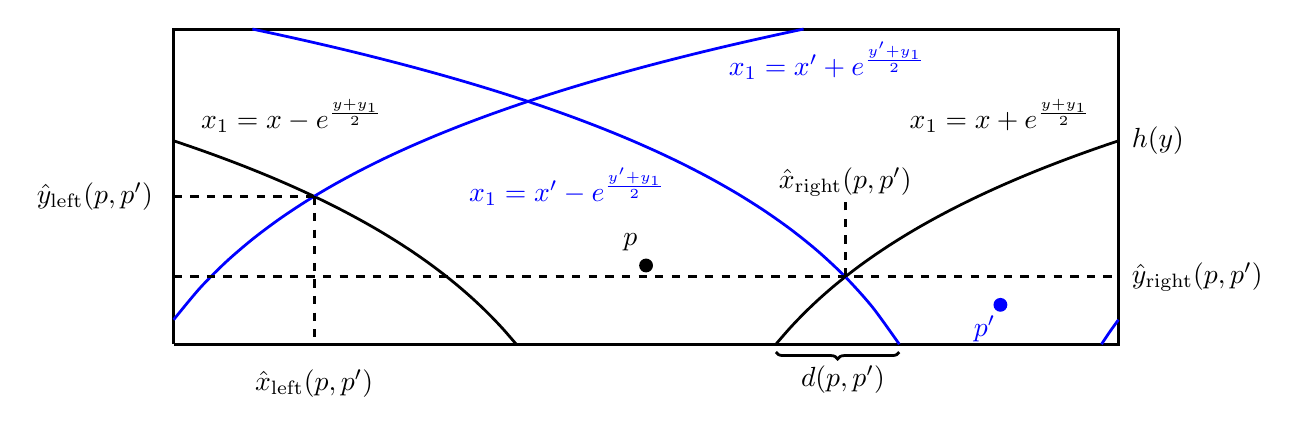
\begin{tikzpicture}
	

	\pgfmathsetmacro{\u}{0} %0
	\pgfmathsetmacro{\v}{1} %1
	\pgfmathsetmacro{\uu}{4.5} %1.4
	\pgfmathsetmacro{\vv}{0.5} %0.8
	\pgfmathsetmacro{\r}{6}
	\pgfmathsetmacro{\t}{4}
	
	%The box \Rcal
	\draw[line width=1pt] (-\r,0) -- (\r,0) -- (\r,\t) -- (-\r,\t) -- (-\r,0);
	
    \draw node[fill, circle, inner sep=0pt, minimum size=5pt] at (\u,\v) {};
    \draw node at (-0.2,1.3) {$p$};
    
    \draw node[fill,blue, circle, inner sep=0pt, minimum size=5pt] at (\uu,\vv) {};
    \draw node at (4.3,0.2) {\color{blue}$p^\prime$};
	
	\draw[domain=1.6487:6,smooth,variable=\x,black,line width=1pt] plot (\x, {2*ln(\x)-1});
    \draw[domain=-1.6487:-6,smooth,variable=\x,black,line width=1pt] plot (\x, {2*ln(-\x)-1});
    \draw[domain=5.7840:6,smooth,variable=\x,blue,line width=1pt] plot (\x, {2*ln(\x-4.5)-0.5});
    \draw[domain=3.2160:-5,smooth,variable=\x,blue,line width=1pt] plot (\x, {2*ln(4.5-\x)-0.5});
    \draw[domain=2:-6,smooth,variable=\x,blue,line width=1pt] plot (\x, {2*ln(\x+7.5)-0.5});
    
    
    
    \draw [decorate,decoration={brace},line width=1pt] (3.2160,-0.1) -- (1.6487,-0.1);
    \draw node at (2.5,-0.45) {$d(p,p^\prime)$};
    
%    \draw [dotted,line width=1pt] (2.5298,0.8563) -- (2.5298,1.7);
%    \draw node at (2.5298,2) {$\hat{x}(p,p^\prime)$};
    
    %Define intersection left black and shifted blue curve
    \pgfmathsetmacro{\vast}{2*ln((2*\r - \uu)/(exp(\v/2) + exp(\vv/2)))}
    \pgfmathsetmacro{\uast}{(\uu - 2*\r)/(1+exp((\vv-\v)/2))}
    %Define intersection right black and left blue curve
    \pgfmathsetmacro{\vvast}{2*ln((\uu)/(exp(\v/2) + exp(\vv/2)))}
    \pgfmathsetmacro{\uuast}{(\u*exp(\vv/2) + \uu*exp(\v/2))/(exp(\v/2) + exp(\vv/2))}
    \pgfmathsetmacro{\h}{2*ln(\r)-\v}
%    \draw[dotted,thick,black] (4.5208,2.0174) -- (4.5208,0);
%    \draw[dotted,thick,black] (4.5208,2.0174) -- (6,2.0174);
    
%    \draw node at (4.5208,-0.5) {$w_x(p,p^\prime)$};
%    \draw node at (7,2.0174) {$w_y(p,p^\prime)$};
    
    \draw node at (\r+0.5,\h) {$h(y)$};
    
    \draw node at (2.3,3.6) {\color{blue}$x_1 = x^\prime + e^{\frac{y^\prime + y_1}{2}}$};
    \draw node at (-1,2) {\color{blue}$x_1 = x^\prime - e^{\frac{y^\prime + y_1}{2}}$};
    \draw node at (-4.5,2.9) {$x_1 = x - e^{\frac{y + y_1}{2}}$};
    \draw node at (4.5,2.9) {$x_1 = x + e^{\frac{y + y_1}{2}}$};
	
	
	\draw[dashed,black,line width=1pt] (-\r,\vast) -- (\uast,\vast);
	\draw node at (-\r-1,\vast) {\color{black}$\hat{y}_{\text{left}}(p,p^\prime)$};
	\draw[dashed,line width=1pt] (\uast,\vast) -- (\uast,0);
	\draw node at (\uast,-0.5) {$\hat{x}_{\text{left}}(p,p^\prime)$};

	\draw[dashed,black,line width=1pt] (-\r,\vvast) -- (\r,\vvast);
	\draw node at (\r+1,\vvast) {\color{black}$\hat{y}_{\text{right}}(p,p^\prime)$};
	\draw[dashed,line width=1pt] (\uuast,\vvast) -- (\uuast,\vvast+1);
	\draw node at (\uuast,\vvast+1.2) {$\hat{x}_{\text{right}}(p,p^\prime)$};
	
	
\end{tikzpicture}
\caption{Schematic representation of the neighbourhoods of $p$ and $p^\prime$ in $\Gbox$ when $|x - x^\prime| > e^{\frac{y}{2}} + e^{\frac{y^\prime}{2}}$ used for the proof of Lemma \ref{lem:common_neighbours_Pcal_n}. Note that although here $p^\prime \notin \BallPon{p}$, this is not true in general. This situation was merely chosen to improve readability of the figure.}
\label{fig:representation_disjoint_neighbourhoods_P_n_3}
\end{figure}


We start by analyzing the shape of the joint neighbourhood. Due to symmetry and the fact that we have identified the left and right boundaries of the box $\Rcal$, we can, without loss of generality, assume that $p = (0,y)$ and $p^\prime = (x^\prime,y^\prime)$ with $x^\prime > 0$. To understand the computation it is helpful to have a picture. Figure~\ref{fig:representation_disjoint_neighbourhoods_P_n_3} shows such an example. There are several different quantities that are important. The first are the heights where the left and right boundaries of the ball $\BallPon{p}$ hit the boundaries of the box $\Rcal$. Since $x = 0$ these heights are the same and we denote their common value by $h(y)$. We also need to know the coordinates $\hat{y}_{\text{right}}(p,p^\prime)$ and $\hat{x}_{\text{right}}(p,p^\prime)$ of the intersection of the right boundary of the neighbourhood of $p$ with the left boundary of the neighbourhood of $p^\prime$ and those for the intersection of the left boundary of the neighbourhood of $p$ with the right boundary of the neighbourhood of $p^\prime$, which we denote by $\hat{y}_{\text{left}}(p,p^\prime)$ and $\hat{x}_{\text{left}}(p,p^\prime)$. Finally we will denote by $d(p,p^\prime)$ the distance between the lower right boundary of $\BallPon{p}$ and the lower left of $\BallPon{p^\prime}$, which is positive only when the bottom parts of both neighbourhoods do not intersect, as is the case in Figure~\ref{fig:representation_disjoint_neighbourhoods_P_n_3}. The condition $d(p,p^\prime) > 0$ is exactly the right notion for $p$ and $p^\prime$ being sufficiently separated.

We start by deriving expressions for these important coordinates. For this we introduce some notation. For any $p = (x,y) \in \Rcal$ we will define the left and right boundary functions as, respectively,
\begin{align}
	b_p^-(z) &= \begin{cases}
		2 \log\left(x-z\right) - y &\mbox{if }  -\frac{\pi}{2} e^{R/2} \le z \le x - e^{y/2}  \\
		2\log\left(\pi e^{R/2} + x - z\right) - y 
			&\mbox{if } x - e^{(y + R)/2} + \pi e^{R/2} \le z \le \frac{\pi}{2} e^{R/2}\\
		0 &\mbox{otherwise}
	\end{cases} \label{eq:def_left_boundary_Bp} \\ 
	b_p^+(z) &= \begin{cases}
		2 \log\left(z-x\right) - y &\mbox{if } x + e^{y/2} \le z \le \frac{\pi}{2} e^{R/2} \\
		2\log\left(\pi e^{R/2} + z - x\right) - y 
			&\mbox{if } -\frac{\pi}{2} e^{R/2} \le z \le x + e^{(y + R)/2} - \pi e^{R/2}\\
		0 &\mbox{otherwise}
	\end{cases}
\end{align}
Note that these functions describe the boundaries of the ball $\BallPon{p}$. In particular, $p^\prime = (x^\prime, y^\prime) \in \BallPon{p}$ if and only if $y^\prime \ge \min\left\{b_p^-(x^\prime), b_p^+(x^\prime)\right\}$.

We shall derive the expressions for the point $(\hat{x}_{\text{left}}(p,p^\prime), \hat{y}_{\text{left}}(p,p^\prime))$. The $x$-coordinate $\hat{x}_{\text{left}}(p,p^\prime)$ is the solution to the equation $b_{p}^+(z) = b_{p^\prime}^-(z)$ for $-\frac{\pi}{2} e^{R/2} \le z \le + e^{y/2}$. This equation becomes
\[
	2\log\left(\pi e^{R/2} + z - x^\prime\right) - y^\prime = 2 \log\left(x^\prime-z\right) - y^\prime,
\]
whose solution is $\frac{x^\prime - \pi e^{R/2}}{1 + e^{(y^\prime - y)/2}}$. Plugging this into either the left or right hand side of the above equation yields the $y$-coordinate $\hat{y}_{\text{left}}(p,p^\prime) = 2 \log\left(\frac{\pi e^{R/2} - x^\prime}{e^{y/2} + e^{y^\prime/2}}\right)$. The expressions for $\hat{x}_{\text{right}}(p,p^\prime$ and $\hat{y}_{\text{right}}(p,p^\prime)$ are derived in a similar way. The expression for $d(p,p^\prime)$ follows as the difference $b_{p^\prime}^-(x^\prime - e^{y^\prime/2}) - b_p^+(e^{y/2})$.

The full expressions of all coordinates are given below for further reference.

\begin{align}
	h(y) &= R - y + 2\log\left(\frac{\pi}{2}\right) \label{eq:def_height_y_P_n}\\
%	h_1(p^\prime) &= 2\log\left(x^\prime + \frac{\pi}{2}e^{\frac{R}{2}}\right) - y^\prime \label{eq:def_height_left_P_n} \\
%	h_2(p^\prime) &= 2\log\left(\frac{\pi}{2}e^{\frac{R}{2}} - x^\prime\right) - y^\prime 
%		\label{eq:def_height_right_P_n} \\
%	\iota_x(p,p^\prime) &= \frac{(x^\prime-x)e^{\frac{y}{2}}}{e^{\frac{y}{2}} - e^{\frac{y^\prime}{2}}}
%		\label{eq:def_x_intersection_close_boundaries}\\
%	\iota_y(p,p^\prime) &= 2\log\left(\frac{x^\prime - x}{e^{\frac{y}{2}} - e^{\frac{y^\prime}{2}}}\right)
%		\label{eq:def_y_intersection_close_boundaries}\\
	\hat{y}_{\text{right}}(p,p^\prime) &= 2\log\left(\frac{x^\prime}{e^{\frac{y}{2}} + e^{\frac{y^\prime}{2}}}\right)\\
	\hat{x}_{\text{right}}(p,p^\prime) &= \frac{x^\prime}{1 + 	
		e^{\frac{y^\prime - y}{2}}},\\
	\hat{y}_{\text{left}}(p,p^\prime) &= 2 \log\left(\frac{\pi e^{R/2} - x^\prime}{e^{\frac{y}{2}} + e^{\frac{y^\prime}{2}}}\right),\\
	\hat{x}_{\text{left}}(p,p^\prime) &= \frac{x^\prime - \pi e^{R/2}}{1 + e^{\frac{y^\prime - y}{2}}}, \\
	d(p,p^\prime) &= |x - x^\prime|_n - \left(e^{\frac{y}{2}} + e^{\frac{y^\prime}{2}}\right).
	\label{eq:def_d_p_p_prime}
\end{align}

The following result shows that if $d(p,p^\prime) > 0$, then the expected number of common neighbours is $\smallO{\Mu{\BallPon{p}} + \Mu{\BallPon{p^\prime}}}$.

\begin{lemma}\label{lem:common_neighbours_Pcal_n}
Let $p, p^\prime \in \Rcal$. Then, whenever $|x - x^\prime|_n > \left(e^{\frac{y}{2}} + e^{\frac{y^\prime}{2}}\right)$,
\[
	\Exp{\Ncal_{\text{box}}(p,p^\prime)} \le \Mu{\BallPon{p}}
	\left(\left(\frac{|x - x^\prime|}{e^{\frac{y}{2}} + e^{\frac{y^\prime}{2}}}\right)^{-(2\alpha - 1)}  
	+ \frac{\nu}{\xi} e^{-(\alpha - \frac{1}{2})(R-y)}\right).
\]
\end{lemma}

\begin{proof}
Again, without loss of generality we assume that $p = p_0 = (0,y)$ and $p^\prime = (x^\prime, y^\prime)$ with $0 \le x^\prime \le \frac{\pi}{2} e^{R/2}$. Note that since $0 < x^\prime \le \frac{\pi}{2} e^{R/2}$, $ \hat{y}_{\mathrm{right}}(p,p^\prime) \le \hat{y}_{\mathrm{left}}(p,p^\prime)$. We write $\hat{y}$ for $\hat{y}_{\mathrm{right}}(p,p^\prime)$ and observe that below $\hat{y}$ the balls $\BallPon{p}$ and $\BallPon{p^\prime}$ are disjoint. Therefore, if we define $A := \left\{p_1 = (x_1,y_1) \in \Rcal \cap \BallPon{p} \, : \, y_1 \ge \hat{y} \right\}$. Then
\[
	\Exp{\Ncal_{\text{box}}(p,p^\prime)} \le \Mu{A}.
\]
We proceed with computing the right hand side
\begin{align*}
	\Mu{A} &= \int_{\hat{y}}^{h(y)} 
		\int_{- e^{\frac{y + y_1}{2}}}^{e^{\frac{y^\prime+y_1}{2}}} 
		f(x_1,y_1) \dd x_1 \dd y_1
		+ \int_{h(y)}^{R} \int_{-\frac{\pi}{2}e^{R/2}}^{\frac{\pi}{2} e^{R/2}} 
		\hspace{-10pt}  f(x_1,y_1) \dd x_1 \dd y_1 \\
	&= \frac{2\alpha \nu}{\pi}e^{\frac{y}{2}}
		\int_{\hat{y}}^{h(y)} e^{-(\alpha - \frac{1}{2})y_1} \dd y_1 
		+ \alpha \nu e^{R/2} \int_{h(y)}^R e^{-\alpha y_1} \dd y_1\\
	&\le \xi\left(e^{\frac{y}{2}} + e^{\frac{y^\prime}{2}}\right) e^{-(\alpha-\frac{1}{2})\hat{y}}
		+ \nu e^{R/2} e^{-\alpha h(y)} \\
	&= \Mu{\BallPon{p}}\left(
		e^{-(\alpha-\frac{1}{2})\hat{y}} + \frac{\nu}{\xi} e^{-(\alpha - \frac{1}{2})(R-y)}\right).
\end{align*}
The result follows by plugging in 
\[
	\hat{y} := \hat{y}_{\text{right}}(p,p^\prime) = 2 \log\left(\frac{x^\prime}{e^{\frac{y}{2}} + e^{\frac{y^\prime}{2}}}\right),
\]
and noting that $x^\prime$ is the same as $|x - x^\prime|$, by our generalization step.

\end{proof} 

We can also prove a similar result for the Poissonized KPKVB model $\GPo$, denoting by $\Ncal_{\Po}(p,p^\prime)$ the number of joint neighbours in $\GPo \cup \{p,p^\prime\}$.

\begin{lemma}\label{lem:common_neighbours_KPKVB}
Let $0 < \varepsilon < 1$, $p, p^\prime \in \Rcal$ with $y,y^\prime \le (1-\varepsilon)R$, denote by $\Ncal_{\Po}(p,p^\prime)$ the number of joint neighbours of $p, p^\prime$ in $\GPo$ and let $K$ be the constant from Lemma~\ref{lem:asymptotics_Omega_hyperbolic}. Then, whenever $|x - x^\prime|_n > \left(e^{\frac{y}{2}} + e^{\frac{y^\prime}{2}}\right)\left(1 + \frac{\pi^2 K}{4}\right)$,
\[
	\Exp{\Ncal_{\Po}(p,p^\prime)} \le \Mu{\BallHyp{p}}
	\left(e^{(2\alpha - 1)\lambda} \left(\frac{|x - x^\prime|}{e^{\frac{y}{2}} + e^{\frac{y^\prime}{2}}}\right)^{-(2\alpha - 1)}  
	+ \frac{\nu}{\xi} e^{-(\alpha - \frac{1}{2})(R-y)}\right),
\]
where
\[
	\lambda = \log\left(1 + \frac{\pi^2 K}{4}\right).
\]
\end{lemma}

\begin{proof}
We will proceed in a similar fashion as for Lemma~\ref{lem:common_neighbours_Pcal_n}. That is, we will bound the expected number of common neighbours by the number of neighbors of $p$ whose $y$-coordinate is above the intersection of the right boundary of $\BallHyp{p}$ and the left boundary of $\BallHyp{p^\prime}$. Denote by $\hat{y}$ the height of this intersection point. Then
\begin{align*}
	\Exp{\Ncal_{\Po}(p,p^\prime)} &\le \frac{2\alpha \nu}{\pi} \int_{\hat{y}}^{R-y} \Phi(y,y_1) e^{-\alpha y_1} \dd y_1
		+ \alpha \nu e^{R/2} \int_{R-y}^{R} e^{-\alpha y_1} \dd y_1.
\end{align*} 
The second integral is bounded by $\frac{\nu}{\xi} \Mu{\BallPon{y}} e^{-(\alpha - \frac{1}{2})(R-y)}$. We bound the first integral using Lemma~\ref{lem:asymptotics_Omega_hyperbolic} as
\begin{align*}
	\frac{2\alpha \nu}{\pi} \int_{\hat{y}}^{R-y} \Phi(y,y_1) e^{-\alpha y_1} \dd y_1
	&\le \frac{2\alpha \nu}{\pi} \int_{\hat{y}}^{R-y} \left(e^{\frac{y+y_1}{2}} + K e^{\frac{3}{2}(y + y_1)-R}\right) 
		e^{-\alpha y_1} \dd y_1 \\
	&\le \frac{2\alpha \nu}{\pi} (1+K)e^{\frac{y}{2}} \int_{\hat{y}}^{R-y} e^{-(\alpha - \frac{1}{2}) y_1} \dd y_1\\
	&\le (1 + K)\Mu{\BallPon{p}}  e^{-(\alpha - \frac{1}{2})\hat{y}},
\end{align*}
where we used that $\frac{3y_1}{2} \le R - y + \frac{y_1}{2}$ for all $y_1 \le R-y$ for the second line. 

It remains to compute $\hat{y}$, for which we will establish the following bound
\begin{equation}\label{eq:joint_neighbors_KPKVB_intersection}
	\hat{y} \ge 2 \log\left(\frac{x^\prime}{e^{\frac{y}{2}} + e^{\frac{y^\prime}{2}}}\right) - 2\lambda.
\end{equation}

To show~\eqref{eq:joint_neighbors_KPKVB_intersection} we note that for any point $y_1 \ge \hat{y}$, the corresponding $x$-coordinate of the left boundary of $\BallHyp{p^\prime}$ must be to the left of that of the ball $\BallHyp{p}$, i.e.
$x^\prime - \Phi(y^\prime, y_1) \le \Phi(y,y_1)$. Therefore it is enough to show that for all 
\[
	y_1 \le 2 \log\left(\frac{x^\prime}{e^{\frac{y}{2}} + e^{\frac{y^\prime}{2}}}\right) - 2\lambda
\]
it holds that $\Phi(y,y_1) \le x^\prime - \Phi(y^\prime, y_1)$, with $\lambda$ as defined in the statement of the lemma. Note that by assumption on $x^\prime := |x - x^\prime|_n$ (since we can take $x = 0$) the above upper bound is non-negative. Using Lemma~\ref{lem:asymptotics_Omega_hyperbolic} it suffices to prove that for all such $y_1$,
\[
	e^{\frac{y + y_1}{2}} + K e^{\frac{3}{2}(y + y_1) - R} \le x^\prime - e^{\frac{y^\prime + y_1}{2}}
	- K e^{\frac{3}{2}(y^\prime + y_1) - R},
\]
which is equivalent to
\[
	\left(e^{\frac{y}{2}} + e^{\frac{y^\prime}{2}}\right) e^{\frac{y_1}{2}} 
	+ K e^{-R} \left(e^{\frac{y}{2}} + e^{\frac{y^\prime}{2}}\right)^3 e^{\frac{3 y_1}{2}} \le x^\prime.
\]
Plugging the upper bound for $y_1$ into the left hand side and using that $(e^{y/2} + e^{y^\prime/2})^3 \ge e^{3y/2} + e^{3y^\prime/2}$, we obtain
\begin{align*}
	\left(e^{\frac{y}{2}} + e^{\frac{y^\prime}{2}}\right) e^{\frac{y_1}{2}} 
		+ K e^{-R} \left(e^{\frac{y}{2}} + e^{\frac{y^\prime}{2}}\right)^3 e^{\frac{3 y_1}{2}}
	&\le x^\prime e^{-\lambda} + K e^{-R} (x^\prime)^3 e^{-3\lambda}
		\le x^\prime \left(e^{-\lambda} + \frac{\pi^2 K}{4} e^{-3\lambda}\right)\\
	&\le x^\prime e^{-\lambda} \left(1 + \frac{\pi^2 K}{4}\right) = x^\prime,
\end{align*} 
where we also used that $x^\prime \le \frac{\pi}{2} e^{-R/2}$.
\end{proof}

Let us now define the \emph{stripe}
\begin{equation}\label{eq:def_stripe}
	\stripknc = \Rcal \cap (\R_+ \times \Kcal_C(k_n)).
\end{equation} 
and in addition define, for any $0 < \varepsilon < 1$, the following set
\begin{equation}\label{eq:def_joint_degree_set_E_growing_k}
	\mathcal{E}_{\varepsilon}(k_n) = \left\{(p,p^\prime) \in \stripknc
		\, : \,  |x - x^\prime|_n > k_n^{1 + \varepsilon} \right\}, 
\end{equation}
where $|x|_n = \min\{|x|, \pi e^{R/2} - |x|\}$ denotes the norm on the finite box $\Rcal$ where the left and right boundaries are identified. Then for any two points $p,p^\prime \in \mathcal{E}_\varepsilon(k_n)$ the expect number of joint neighbours is $\smallO{k_n}$.

\begin{lemma}\label{cor:expected_common_neighbours_Ecal_set}
Fix $0 < \varepsilon < 1$ and let $\varepsilon^\prime = \min\{\varepsilon(2\alpha - 1),\varepsilon\}$. Then for all $(p,p^\prime) \in \mathcal{E}_\varepsilon(k_n)$, as $n \to \infty$,
\[
	\Mu{\BallPon{p} \cap \BallPon{p^\prime}} = \bigO{k_n^{1-\varepsilon^\prime}}.
\] 
\end{lemma}

\begin{proof}
Since for all $(p,p^\prime) \in \mathcal{E}_\varepsilon(k_n)$ we have $\Mu{\BallPon{p}}, \Mu{\BallPon{p^\prime}} = \bigT{k_n}$, Lemma~\ref{lem:common_neighbours_Pcal_n} implies that
\[
	\Mu{\BallPon{p} \cap \BallPon{p^\prime}} \le \bigO{k_n} \phi_n(p,p^\prime),
\]
where
\[
	\phi_n(p,p^\prime) = 2\left(\frac{|x - x^\prime|_n}{e^{\frac{y}{2}} + e^{\frac{y^\prime}{2}}}\right)^{-(2\alpha - 1)} 
		+ \frac{3 \nu^{2\alpha + 1}e^{-(\alpha - \frac{1}{2})R} e^{\alpha y}}{2 \pi^{2\alpha}\left(
		e^{\frac{y}{2}} + e^{\frac{y^\prime}{2}}\right)}
		+ \frac{\nu e^{-(\alpha - \frac{1}{2})R}}{e^{\frac{y}{2}} + e^{\frac{y^\prime}{2}}}. 
\]
We thus need to show that $\phi_n(p,p^\prime) = \bigO{k_n^{-\varepsilon^\prime}}$. For $(p,p^\prime) \in \mathcal{E}_\varepsilon(k_n)$, it holds that $e^{y/2}, e^{y^\prime/2} = \bigT{k_n}$ and $|x - x^\prime|_n > k_n^{1+\varepsilon}$ and hence
\begin{align*}
	 2\left(\frac{|x - x^\prime|_n}{e^{\frac{y}{2}} + e^{\frac{y^\prime}{2}}}\right)^{-(2\alpha - 1)}
	 =	\bigO{k_n^{-\varepsilon(2\alpha - 1)}}.
\end{align*}
For the second term in $\phi_n(p,p^\prime)$ we use that $e^{\alpha y^\ast} = \bigT{k_n^{2\alpha}}$ and $e^{R} = \bigT{n^2}$ to obtain
\[
	\frac{3 \nu^{2\alpha + 1}e^{-(\alpha - \frac{1}{2})R} e^{\alpha y}}{2 \pi^{2\alpha}\left(
			e^{\frac{y}{2}} + e^{\frac{y^\prime}{2}}\right)}
	= \bigO{1} n^{-(2\alpha - 1)} k_n^{2\alpha - 1} = \bigO{n^{-(\alpha - \frac{1}{2})}}.
\]
Finally, the third term satisfies $\bigO{n^{-(2\alpha - 1)}k_n^{-1}}$, and we conclude that
\[
	\phi_n(p,p^\prime) = \bigO{k_n^{-\varepsilon(2\alpha - 1)} + n^{-(\alpha - \frac{1}{2})}
	+ n^{-(2\alpha - 1)}k_n^{-1}} = \bigO{k_n^{-\varepsilon^\prime}},
\]
where we used that $\varepsilon^\prime = \min\{\varepsilon(2\alpha - 1),\varepsilon\}$. 
\end{proof}

It is clear that using Lemma~\ref{lem:common_neighbours_KPKVB} instead of Lemma~\ref{lem:common_neighbours_Pcal_n}, the above proof applies to the Poissonized KPKVB model, yielding the following result.

\begin{lemma}\label{cor:expected_common_neighbours_KPKVB}
Fix $0 < \varepsilon < 1$ and let $\varepsilon^\prime = \min\{\varepsilon(2\alpha - 1),\varepsilon\}$. Then for all $(p,p^\prime) \in \mathcal{E}_\varepsilon(k_n)$, as $n \to \infty$,
\[
	\Mu{\BallHyp{p} \cap \BallHyp{p^\prime}} = \bigO{k_n^{1-\varepsilon^\prime}}.
\] 
\end{lemma}

Recall the definition of the stripe $\stripknc = \Rcal \cap (\R_+ \times [y_{k_n,C}^-, y_{k_n,C}^+])$ from~\eqref{eq:def_stripe}. Consider a fixed number of points $p_1, \dots, p_r$. Then, if their $x$-coordinates are sufficient far apart and their $y$ coordinates lie within the stripe $\stripknc$, their degrees are asymptotically independent.

\begin{lemma}[Asymptotic factorization of degree probabilities]\label{lem:probdegFact}
Let $(k_n)$ be a sequence of integers with $0\leq k_n \leq n-1$, $k_n = \bigO{n^{\frac{1}{2\alpha+1}}}$ and $k_n \rightarrow \infty$.
Let $C, C^\prime>0$ and $r,s$ be positive integers with $r+1\leq s$. Fix $0<\varepsilon<1$. Then, it holds uniformly for all $(v_1,\dots,v_s) \in \left(\stripknc\right)^{s} = \stripknc \times \dots \times \stripknc$, satisfying $|x_{v_i}-x_{v_{r+1}}|\geq k_n^{1+\varepsilon}$ for all  $1\leq i \leq r$,  that
\[
	\varphi(\{v_1,\dots,v_{r+1}\};v_1,\dots,v_s)
	=(1+o(1))\varphi(\{v_1,\dots,v_r\};v_1,\dots,v_s)\varphi(\{v_{r+1}\};v_1,\dots,v_s)+\bigO{k_n^{-C^\prime}},
\]
where $\varphi$ is either $\varphi_{\Po}$ or $\varphi_{\mathrm{box}}$.
(Here uniformity means that the $\smallO{1}$ and $\bigO{k_n}$ terms do not depend on $v_1,\dots,v_{s}$.)
\end{lemma}

\begin{proof}
Let $H=\GPo \cup\{p_1,\dots,p_s\}$ or $H=\Gbox \cup \{p_1,\dots,p_s\}$ and $1\leq r\leq s$. For $1\leq j \leq r$, let $Y_j$ be the number of vertices of $H$ which are adjacent to both $p_j$ and $p_{r+1}$. Let $X_j$ be the number of vertices of $H$ which are adjacent to $p_j$, but not to $p_{r+1}$. Then, $X_j+Y_j= D_{H}(p_j)$ is the degree of $p_j$ in $H$. 

Now let $X_{r+1}$ be the number of vertices of $H$ which are adjacent to $p_{r+1}$, but to none of $p_1,\dots,p_r$. Let $Y_{r+1}$ be the number of vertices of $H$ which are adjacent to $p_{r+1}$, and at least one of $p_1,\dots,p_r$. Then, $X_{r+1}+Y_{r+1}=D_H(p_{r+1})$ is the degree of $p_{r+1}$ in $H$. By definition, we therefore have
\begin{align*}
\varphi(\{p_1,\dots,p_{r+1}\};p_1,\dots,p_s)&=\Prob{X_1+Y_1=\dots=X_{r+1}+Y_{r+1}=k_n}, \\
\varphi(\{p_1,\dots,p_r\};p_1,\dots,p_s)&=\Prob{X_1+Y_1=\dots=X_r+Y_r=k_n}, \\
\varphi(\{p_{r+1}\};p_1,\dots,p_s)&=\Prob{X_{r+1}+Y_{r+1}=k_n},
\end{align*}
and the claim of the lemma is that
\begin{equation}\label{eq:probdegfact_main}
	\begin{aligned}
		&\Prob{X_1+Y_1=\dots=X_{r+1}+Y_{r+1}=k_n} \\
		&= (1+o(1))\Prob{X_1+Y_1=\dots=X_r+Y_r=k_n}\Prob{X_{r+1}+Y_{r+1}=k_n}+\bigO{k_n^{-C}}.
	\end{aligned}
\end{equation}

To prove~\eqref{eq:probdegfact_main} let $\varepsilon'=\min(\varepsilon,\varepsilon(2\alpha-1))\in (0,1)$. Since for $1\leq i \leq r$, it is given that $|x_{p_i}-x_{p_{r+1}}|\geq k_n^{1+\varepsilon}$, then in the case where $H = \GPo \cup\{p_1,\dots,p_s\}$ it follows from Lemma~\ref{lem:common_neighbours_KPKVB} that $\E[Y_j] = \bigO{k_n^{1-\varepsilon'}}$. When $H=\Gbox \cup \{p_1,\dots,p_s\}$ we get the same result using Lemma~\ref{lem:common_neighbours_Pcal_n}. The rest of the proof is independent of which of the two models we consider and only uses that $\E[Y_j] = \bigO{k_n^{1-\varepsilon'}}$.

As $Y_{r+1} \leq Y_1+\dots+Y_r$, we also have $\mu:=\Exp{Y_{r+1}} = \bigO{k_n^{1-\varepsilon'}}$. In particular, there is $c_0>0$ such that $c_0\sqrt{k_n^{1-\varepsilon'}\ln k_n^{1-\varepsilon'}}\geq c_1\sqrt{\mu\ln\mu}$ (where $c_1=\sqrt{\frac{2C}{1-\varepsilon'}}$, which is well-defined because $1-\varepsilon'>0$). Now define
\begin{align*}
A_n=[\mu-c_0\sqrt{k_n^{1-\varepsilon'}\ln k_n^{1-\varepsilon'}},\mu+c_0\sqrt{k_n^{1-\varepsilon'}\ln k_n^{1-\varepsilon'}}]\cap \N_0.%=[\mu-c\sqrt{\mu\ln \mu},\mu+c\sqrt{\mu\ln \mu}].
\end{align*}
By equation~\eqref{eq:def_chernoff_bound_poisson_C}, we have
\begin{align*}
	\Prob{Y_{r+1} \not \in A_n} 
	&= \Prob{|Y_{r+1}-\mu|\geq c_0\sqrt{k_n^{1-\varepsilon'}\ln k_n^{1-\varepsilon'}}}\\
	&\le \Prob{|Y_{r+1}-\mu|\geq c_1\sqrt{\mu\ln\mu}}
	=\bigO{k_n^{-\frac{(1-\varepsilon')c_1^2}{2}}}.
\end{align*}
As by definition $c_1$ satisfies $\frac{(1-\varepsilon')c_1^2}{2}=C$, this implies that for the event $S_n = \{Y_{r+1}\in A_n\}$,
\[
	\Prob{S_n^c}=\bigO{k_n^{-C}}.
\]
Beginning with the left-hand side of the claim of the lemma, the law of total probability applied to the events $\{Y_{r+1}=y_{r+1}\}$, for all $y_{r+1}\in A_n$, and $S_n^c$ implies that
\begin{align*}
	&\Prob{X_1+Y_1=\dots=X_{r+1}+Y_{r+1}=k_n} \\
	&=\sum_{y_{r+1}\in A_n} \Prob{X_1+Y_1=\dots=X_{r+1}+y_{r+1}=k_n|Y_{r+1}=y_{r+1}}\Prob{Y_{r+1}=y_{r+1}}\\ 
	&\hspace{10pt}+ \Prob{X_1+Y_1=\dots=X_{r+1}+Y_{r+1}=k_n|S_n^c} \Prob{S_n^c}\\
	&=\sum_{y_{r+1}\in A_n} \Prob{X_1+Y_1=\dots=X_{r+1}+y_{r+1}=k_n|Y_{r+1}=y_{r+1}} 
		\Prob{Y_{r+1}=y_{r+1}}+\bigO{k_n^{-C}}.
\end{align*}
As $X_{r+1}$ is independent of $X_1, \dots, X_r, Y_1, \dots, Y_r$ by the properties of a Poisson process (as $X_{r+1}$ counts the number of points in a set which is disjoint of $X_1,\dots,X_r, Y_1, \dots, Y_r$), it follows that
\begin{align*}%\label{eq:afterindep}
	&\Prob{X_1+Y_1=\dots=X_{r+1}+Y_{r+1}=k_n} \\
	&=\sum_{y_{r+1} \in A_n} \Prob{X_1+Y_1=\dots=X_{r}+Y_r=k_n|Y_{r+1}=y_{r+1}}
		\Prob{X_{r+1}+y_{r+1}=k_n} \Prob{Y_{r+1}=y_{r+1}}\\
	&\hspace{10pt} +\bigO{k_n^{-C}}.
\end{align*}
We will now show that uniformly for all $y_{r+1}, s \in A_n$, it holds that,
\begin{align}\label{eq:yrp1tos}
	\Prob{X_{r+1}=k_n-y_{r+1}} = (1+o(1))\Prob{X_{r+1}=k_n-s}.
\end{align}
To see this, observe that for all $y_{r+1},s\in A_n$, we have that $|y_{r+1}-s|\leq 2c\sqrt{k_n^{1-\varepsilon'}\ln k_n^{1-\varepsilon'}}$. Denote the expectation of $X_{r+1}$ by $\lambda$, write $\delta_n = k_n-y_{r+1}-\lambda$ and note that
\begin{align*}
	\frac{\Prob{X_{r+1}=k_n-y_{r+1}}}{\Prob{X_{r+1}=k_n-s}} 
	&= \frac{\Prob{X_{r+1}=k_n-y_{r+1}}}{\Prob{X_{r+1}=k_n-y_{r+1}+(y_{r+1}-s)}}\\
	&=\frac{(k_n-y_{r+1}+(y_{r+1}-s))!}{(k_n-y_{r+1})!}\lambda^{s-y_{r+1}}
\end{align*}
We will now use that $\frac{(a+b)!}{a!} = (1+o(1))(a+b)^b$ for $b^2=o(a)$, applied to $a=k_n-y_{r+1}$ and $b=y_{r+1}-s$. To see this auxiliary fact, note that by Stirling's approximation to the factorial (see e.g.~\cite{Dutkay2013},~\cite{Nanjundiah1959}), it follows that
\begin{align*}
	\frac{(a+b)!}{a!}=(1+o(1))\frac{(a+b)^{a+b+\frac{1}{2}}e^{-a-b}}{a^{a+\frac{1}{2}}e^{-a}}
	=(1+o(1))\left(1+\frac{b}{a}\right)^{a+\frac{1}{2}}(a+b)^b e^{-b}.
\end{align*}
Since $1+\frac{b}{a}\leq e^{\frac{b}{a}}$, it holds that $(1+\frac{b}{a})^a \leq e^b$. Furthermore, as $\ln(1+x)\geq x-\frac{x^2}{2}$ (for $x\in (-1,1)$), we have that $(1+\frac{b}{a})^a =e^{a\ln(1+\frac{b}{a})}\geq e^{a(\frac{b}{a}-\frac{b^2}{2a})} =e^{b-\frac{b^2}{2a}}=(1+o(1))e^{b}$ because $b^2=o(a)$. Finally, $b^2=o(a)$ also implies that $(1+\frac{b}{a})^\frac{1}{2}=1+o(1)$. This finishes the proof of the auxiliary fact and we can continue with
\begin{align*}
	\frac{\Prob{X_{r+1}=k_n-y_{r+1}}}{\Prob{X_{r+1}=k_n-s}}
	&=(1+o(1)) (k_n-y_{r+1}+(y_{r+1}-s))^{y_{r+1}-s} \lambda^{s-y_{r+1}} \\
	&=(1+o(1)) (\lambda+\delta_n+(y_{r+1}-s))^{y_{r+1}-s} \lambda^{s-y_{r+1}} \\
	&=(1+o(1))\left(1+\frac{\delta_n+(y_{r+1}-s)}{\lambda}\right)^{y_{r+1}-s} \\
	&=(1+o(1)) e^{\frac{\delta_n(y_{r+1}-s)}{\lambda}} e^{\frac{(y_{r+1}-s)^2}{\lambda}} = 1+o(1),
\end{align*}
where the last line follows since $\delta_n, |y_{r+1}-s| \leq 2c_0\sqrt{k_n^{1-\varepsilon'}\ln k_n^{1-\varepsilon'}}$ and $\lambda=\Theta(k_n)$ and therefore, with convergence uniform in $y_{r+1},s$,
\[
	\frac{\delta_n(y_{r+1}-s)}{\lambda}, \frac{(y_{r+1}-s)^2}{\lambda} \leq \frac{4c_0^2 k_n^{1-\varepsilon'}\ln k_n^{1-\varepsilon'}}{\lambda}  \rightarrow 0.
\]
As $\Prob{S_n^c}=\bigO{k_n^{-C}}$, we have
\begin{align*}
	1=\sum_{s\in A_n}\Prob{Y_{r+1}=s}+\bigO{k_n^{-C}}.
\end{align*}
From~\eqref{eq:yrp1tos}, it then follows that
\begin{align*}
	\Prob{X_{r+1}=k_n-y_{r+1}} 
	&=\Prob{X_{r+1}=k_n-y_{r+1}} \sum_{s\in A_n} \Prob{Y_{r+1}=s}+\bigO{k_n^{-C}}\\
	&= (1+o(1)) \sum_{s\in A_n} \Prob{Y_{r+1}=s} \Prob{X_{r+1}=k_n-s}+\bigO{k_n^{-C}} \\
	&=(1+o(1))\sum_{s\in A_n} \Prob{X_{r+1}+Y_{r+1}=k_n, Y_{r+1}=s}+\bigO{k_n^{-C}} \\
	&=(1+o(1))\Prob{X_{r+1}+Y_{r+1}=k_n, Y_{r+1}\in A_n}+\bigO{k_n^{-C}} \\
	&=(1+o(1))\left(\Prob{X_{r+1}+Y_{r+1}=k_n}-\Prob{X_{r+1}+Y_{r+1}=k_n, Y_{r+1}\not \in A_n}\right)+\bigO{k_n^{-C}} \\
	&=(1+o(1))\Prob{X_{r+1}+Y_{r+1}=k_n}+\bigO{k_n^{-C}}.
\end{align*}
Note that $\Prob{X_{r+1}+Y_{r+1}=k_n}$ no longer depends on $y_{r+1}$ and neither does the $\bigO{k_n^{-C}}$ error term. Therefore we have
\begin{align*}
	&\Prob{X_1+Y_1=\dots=X_{r+1}+Y_{r+1}=k_n} \\
	&\sum_{y_{r+1} \in A_n} \Prob{X_1+Y_1=\dots=X_{r}+Y_r=k_n|Y_{r+1}=y_{r+1}} 	
		\Prob{X_{r+1}+y_{r+1}=k_n}\Prob{Y_{r+1}=y_{r+1}}+\bigO{k_n^{-C}}\\
	&=(1+o(1))\Prob{X_{r+1}+Y_{r+1}=k_n}\sum_{y_{r+1} \in A_n} 	
		\Prob{X_1+Y_1=\dots=X_{r}+Y_r=k_n|Y_{r+1}=y_{r+1}}\Prob{Y_{r+1}=y_{r+1}}\\
	&\hspace{10pt}+\bigO{k_n^{-C}}.
\end{align*}
For the last summation we have
\begin{align*}
	&\sum_{y_{r+1} \in A_n} \Prob{X_1+Y_1=\dots=X_{r}+Y_r=k_n|Y_{r+1}=y_{r+1}}\Prob{Y_{r+1}=y_{r+1}} \\
	&= \Prob{X_1+Y_1=\dots=X_r+Y_r=k_n,Y_{r+1}\in A_n} \\
	&= (1+o(1))\Prob{X_1+Y_1=\dots=X_r+Y_r=k_n}+\bigO{k_n^{-C}}.
\end{align*}
Finally, plugging this into the previous step gives 
\begin{align*}
	&\Prob{X_1+Y_1=\dots=X_{r+1}+Y_{r+1}=k_n} \\
	&=(1+o(1))\Prob{X_{r+1}+Y_{r+1}=k_n}\sum_{y_{r+1} \in A_n} 	
		\Prob{X_1+Y_1=\dots=X_{r}+Y_r=k_n|Y_{r+1}=y_{r+1}}\Prob{Y_{r+1}=y_{r+1}}\\
	&\hspace{10pt}+\bigO{k_n^{-C}} \\
	&=(1+o(1))\Prob{X_{r+1}+Y_{r+1}=k_n}\Prob{X_1+Y_1=\dots=X_r+Y_r=k_n}+\bigO{k_n^{-C}}.
\end{align*}
which establishes~\eqref{eq:probdegfact_main} and thus the claim of the lemma.
\end{proof}

\subsection{Factorial moments of degrees}\label{ssec:factorial_moments_GPo}

Now that we have analyzed the joint neighbourhoods and degree distributions in both the Poissonized KPKVB and finite box model, we can show convergence of the factorial moments of the number of nodes of degree $k$ in both models.

\begin{lemma}[Factorial moments]\label{lem:factmoment}
Recall that $N_{Po}(k)$ denotes the number of degree $k$ vertices in $\GPo$. Let $(k_n)$ be a sequence of integers with $0\leq k_n \leq n-1$, $k_n = \bigO{n^{\frac{1}{2\alpha+1}}}$ and $k_n \rightarrow \infty$. Then, for any positive integer $r$, it holds that
\[
	\Exp{{N_{Po}(k_n) \choose r}} =(1+o(1)) \frac{(\Exp{ N_{Po}(k_n)})^r}{r!}.
\]
\end{lemma}

The proof of this result requires the following technical lemma which states that the integration of the joint degree distribution can be factorized.

\begin{lemma}[Factorization of degrees]
	\label{lem:asympind}
	Let $(k_n)$ be a sequence of integers with $0\leq k_n \leq n-1$, $k_n = \bigO{n^{\frac{1}{2\alpha+1}}}$ and $k_n \rightarrow \infty$.
	
	Let $\varphi$ be either $\varphi_{\mathrm{box}}$ or $\varphi_{\Po}$. Then we have that
	\begin{align*}
	&\int_\Rcal \cdots \int_\Rcal \varphi(\{p_1,\dots,p_r \}, k_n ;p_1,\dots,p_r) 
		 \dd \mu(p_1) \cdots \dd \mu(p_r) \\
	&= (1+o(1))\left(\int_\Rcal  \varphi(\{p_1\}, k_n ;p_1) \dd \mu(p)\right)^r .
	\end{align*}
\end{lemma}

\begin{proof}
Let $C>r(2\alpha+1)$ and define the set $A = (\Rcal \times \cdots \times\Rcal) \backslash (\stripknc \times \cdots\times \stripknc)$. We will first show that the contribution of the integration of $\varphi$ over this range is negligible. 

For $(p_1,\dots,p_r) \in (\Rcal \times \cdots \times\Rcal) \backslash (\stripknc \times \cdots\times \stripknc)$, there is a $j$, $1\leq j\leq r$, such that $y_j \not \in [y_{k_n,c}^-,y_{k_n,c}^+]$, so that the Chernoff bound (see in~\ref{eq:chernoff_bound_degrees}) yields that $\Prob{D_{\GPo}(v_j)=k_n } = \bigO{k_n^{-C}}$. As, for $1\leq j\leq r$, the event $\{D_{\GPo}(p_1)=\dots=D_{\GPo}(p_r)=k_n\}$ implies the event $\{D_{\GPo}(v_j)=k_n\}$, it follows that $\Prob{D_{\GPo}(p_1)=\dots=D_{\GPo}(p_r)=k_n} = \bigO{k_n^{-C}}$ and hence,
\begin{align*}
	\int_A \Pee(D_{\GPo}(p_1)=\dots=D_{\GPo}(p_r)=k_n) \dd \mu(p_1) \cdots \dd \mu(p_r)	= O\left(n^r k_n^{-C}\right).
\end{align*}

Next we note that by the concentration of heights (Proposition~\ref{prop:concentration_height_general}) it follows that
\begin{align*}
	\int_{\stripknc} \varphi(\{p_1\}, k_n ;p_1) \dd \mu(p_1) 
	&= (1+\smallO{1}) \int_\Rcal  \varphi(\{p_1\}, k_n ;p_1) \dd \mu(p_1) \\
	&= (1+\smallO{1}) 2\alpha \xi^{2\alpha} n k_n^{-(2\alpha + 1)} \numberthis \label{eq:integration_average_degree_stripe}
\end{align*}
Since for $C>r(2\alpha+1)$ it holds that $n^r k_n^{-C} = \smallO{\left(n k_n^{-(2\alpha + 1)}\right)^r}$ it now suffices to show that
\begin{align*}
	&\int_{\stripknc} \cdots \int_{\stripknc} \varphi(\{p_1,\dots,p_r \}, k_n ;p_1,\dots,p_r) 
		\dd \mu(p_1)\cdots \dd \mu(p_r) \\
	&= (1+o(1))\left(\int_{\stripknc}  \varphi(\{p_1\}, k_n ;p_1) \dd \mu(p_1) \right)^r.
\end{align*}

We will prove this using induction. More precisely, for every fixed positive integer $s$, we will show by induction on $r$, $1\leq r\leq s$, that for all $p_{r+1},\dots,p_s \in \stripknc$, it holds that
\begin{align*}
	&\int_{\stripknc} \cdots \int_{\stripknc} \varphi(\{p_1,\dots,p_r\}, k_n ;p_1,\dots,p_s)
		\dd \mu(p_1) \cdots \dd \mu(p_r)\\
	&= (1+o(1))\left(\int_{\stripknc} \varphi(\{p_1\}, k_n ;p_1) \dd \mu(p_1)\right)^r .
\end{align*}
Note that for $r=s$ this is the claim of the lemma. Throughout the proof $H$ is either $\GPo \cup\{p_1,\dots,p_s\}$ or $\Gbox \cup \{p_1,\dots,p_s\}$, depending on whether $\varphi$ is, respectively, $\varphi_{\Po}$ or $\varphi_{\mathrm{box}}$.

For $r=1$, we only need to show that uniformly for $p_1 \in \stripknc$,
\begin{align*}
\varphi(\{p_1\}, k_n ;p_1,\dots,p_s) = (1+o(1))\varphi(\{p_1\}, k_n ;p_1).
\end{align*}
To see this, note that as $p_1\in \stripknc$, the expected degree of $p_1$ in $\GPo$ is $\Theta(k_n)$. Assume that $p_1$ is adjacent to $s'<s$ many vertices among $p_2,\dots,p_s$. Then, as $s'<s$ is bounded and $k_n \rightarrow \infty$ as $n\rightarrow \infty$,  we have that
\begin{align*}
\Pee(D_{\GPo}(p_1)=k_n-s') = (1+o(1))\Pee(D_{\GPo}(p_1)=k_n).
\end{align*}
So, we have the base case of the induction,
\begin{align*}
\varphi(\{p_1\}, k_n ;p_1,\dots,p_s)&=\Pee(D_H(p_1)=k_n)
= \Pee(D_{\GPo}(p_1)=k_n-s')\\
&= (1+o(1))\Pee(D_{\GPo}(p_1)=k_n)=(1+o(1))\varphi(\{p_1\}, k_n ;p_1).
\end{align*}
Assuming the claim holds for integer $r <s$, we will show that it holds for $r+1$.

Let $p_{r+2},\dots,p_s\in \stripknc$ (if $r+2>s$, this definition is void and the corresponding points will never be used in the proof).
Fix $0<\epsilon<1$ small enough s.t. $\frac{1}{2}+\epsilon<\alpha$. Define the region that the $(r+1)$-th vertex $p_{r+1}$ is far apart from all other vertices horizontally,
$$\Fcal_\epsilon(k_n)=\{(p_1,\dots,p_{r+1}) \in \left(\stripknc\right)^{r+1}: \forall 1\leq i \leq r: |x_{p_i}-x_{p_{r+1}}|\geq k_n^{1+\epsilon}\}.$$

We will split the integration into this region and its complement $\Fcal_\epsilon(k_n)^c = \left(\stripknc\right)^{r+1} \backslash \Fcal_\epsilon(k_n)$.

Firstly, we derive an upper bound for the complement $\Fcal_\epsilon(k_n)^c$. Note that 
\[
	\varphi(\{p_1,\dots,p_{r+1}\}, k_n ;p_1,\dots,p_s) \leq \varphi(\{p_1,\dots,p_r\}, k_n ;p_1,\dots,p_s),
\]
and so,
\begin{align*}
	&\int \int_{\Fcal_\epsilon(k_n)^c} \varphi(\{p_1,\dots,p_{r+1}\}, k_n ;p_1,\dots,p_s)
		\dd \mu(p_1) \cdots \dd \mu(p_{r+1})\\
	&\leq \int \int_{\Fcal_\epsilon(k_n)^c} \varphi(\{p_1,\dots,p_r\}, k_n ;p_1,\dots,p_s)
		\dd \mu(p_1) \cdots \dd \mu(p_{r+1}).
\end{align*}

For $(p_1,\dots,p_{r+1})\in \Fcal_\epsilon(k_n)^c$, we have that $(p_1,\dots,p_r) \in \left(\stripknc\right)^r$ and $p_{r+1}=(x_{r+1},y_{r+1})$ satisfies $y_{k_n,c}^-\leq y_{r+1}\leq y_{k_n,c}^+$ and $x_{r+1}$ falls into an interval $I_n$ of length $2k_n^{1+\epsilon}$.
As the integrand $\varphi(\{p_1,\dots,p_r\};p_1,\dots,p_s)$ is constant in $x_{r+1}$, we can upper bound the corresponding integration as follows,
\begin{align*}
	&\int_{\{(x_{r+1},y_{r+1})\in\stripknc: x_{r+1}\in I_n\}} \varphi(\{p_1,\dots,p_r\}, k_n ;p_1,\dots,p_s) 
		\dd \mu(p_{r+1}) \\
	&= \int_{y_{k_n,c}^-}^{y_{k_n,c}^+} \int_{I_n} \varphi(\{p_1,\dots,p_r\}, k_n ;p_1,\dots,p_s)\frac{\alpha \nu}{\pi} e^{-\alpha y_{r+1}} dx_{r+1}dy_{r+1} \\
	&\leq 2k_n^{1+\epsilon} \varphi(\{p_1,\dots,p_r\}, k_n ;p_1,\dots,p_s)\int_{y_{k_n,c}^-}^{y_{k_n,c}^+}  \frac{\alpha \nu}{\pi} e^{-\alpha y_{r+1}} dy_{r+1}.
\end{align*}
Furthermore, we have that
\begin{align*}
	\int_{y_{k_n,c}^-}^{y_{k_n,c}^+} e^{-\alpha y_{r+1}}dy_{r+1} 
	\leq \int_{y_{k_n,c}^-}^\infty e^{-\alpha y_{r+1}}dy_{r+1} 
	= \bigO{e^{-\alpha y_{k_n,c}^-}} = \bigO{\left( \frac{k_n-c\sqrt{k_n\ln k_n}}{\xi}\right)^{-2\alpha}} 
	= \bigO{k_n^{-2\alpha}}.
\end{align*}
We have thus established that
\begin{align*}
	&\int \int_{\Fcal_\epsilon(k_n)^c} \varphi(\{p_1,\dots,p_r\}, k_n ;p_1,\dots,p_s)
		\dd \mu(p_1) \cdots \dd \mu(p_{r+1})\\
	&\leq \bigO{k_n^{1+\epsilon} k_n^{-2\alpha}}\int_{\stripknc} \cdots \int_{\stripknc} 
		\varphi(\{p_1,\dots,p_r\}, k_n ;p_1,\dots,p_s) \dd \mu(p_1) \cdots \dd \mu(p_{r}).
\end{align*}
The $r$-fold integral can the bounded from above using the induction hypothesis as
\begin{align}\label{eq:indhyp}
	\bigO{k_n^{1+\epsilon-2\alpha}}\left(\int_{\stripknc} \varphi(\{p_1\};p_1) \dd \mu(p_1) \right)^r .
\end{align}
Finally, we use that $k_n^{1+\epsilon-2\alpha} = \smallO{\int_{\stripknc} \varphi(\{p_1\};p_1)\mu_n(dp_1)}$. To see this, we will firstly show that $k_n^{1+\epsilon-2\alpha} = \smallO{nk_n^{-(2\alpha+1)}}$ and then apply~\eqref{eq:integration_average_degree_stripe}, which says that
\begin{align*}
\int_{\stripknc} \varphi(\{p_1\};p_1) \dd \mu(p_1) = \bigT{n k_n^{-(2\alpha+1)}}.
\end{align*}
By our choice of $\epsilon$, we have that $\frac{1}{2}+\epsilon<\alpha$, which implies that $\frac{2+\epsilon}{1+2\alpha}<1$, and hence, using $k_n = \bigO{n^{\frac{1}{2\alpha+1}}}$,
\begin{align*}
\frac{k_n^{1+\epsilon-2\alpha}}{nk_n^{-(2\alpha+1)}} = n^{-1} k_n^{2+\epsilon} = \bigO{n^{-1} n^{\frac{2+\epsilon}{1+2\alpha}}} = \smallO{n^{-1}n}= \smallO{1}.
\end{align*}
Having shown that $k_n^{1+\epsilon-2\alpha} = \smallO{\int_{\stripknc} \varphi(\{p_1\};p_1)\mu_n(dp_1)}$, we therefore conclude from~\eqref{eq:indhyp} that
\begin{align*}
	&\int \int_{\Fcal_\epsilon(k_n)^c} \varphi(\{p_1,\dots,p_r\}, k_n ;p_1,\dots,p_s)
		\dd \mu(p_1) \cdots \dd \mu(p_{r+1})\\
	&=\smallO{\int_{\stripknc} \varphi(\{p_1\}, k_n ;p_1)\mu_n(dp_1)}
		\left(\int_{\stripknc} \varphi(\{p_1\}, k_n ;p_1) \dd \mu(p_1) \right)^r  \\
	&=\smallO{\left(\int_{\stripknc} \varphi(\{p_1\}, k_n ;p_1) \dd \mu(p_1)\right)^{r+1}}.
\end{align*}

For the integration over $\Fcal_\epsilon(k_n)$, recall that by Lemma~\ref{lem:probdegFact}, \[
	\varphi(\{p_1,\dots,p_{r+1}\}, k_n ;p_1,\dots,p_s)
	=(1+o(1))\varphi(\{p_1,\dots,p_r\}, k_n ;p_1,\dots,p_s)
	\varphi(\{p_{r+1}\}, k_n ;p_1,\dots,p_s)+\bigO{k_n^{-C}}.
\]
This implies that
\begin{align*}
	&\int \int_{\Fcal_\epsilon(k_n)} \varphi(\{p_1,\dots,p_{r+1}\}, k_n ;p_1,\dots,p_s) 
		 \dd \mu(p_1) \cdots \dd \mu(p_{r+1})\\
	&=(1+o(1))\int \int_{\Fcal_\epsilon(k_n)} \varphi(\{p_1,\dots,p_r\}, k_n ;p_1,\dots,p_s) 
		\varphi(\{p_{r+1}\};p_1,\dots,p_s) \dd \mu(p_1) \cdots \dd \mu(p_{r+1}) \\
	&\hspace{10pt}+\bigO{k_n^{-C}}\int \int_{\Fcal_\epsilon(k_n)} 
		\dd \mu(p_1) \cdots \dd \mu(p_{r+1}) =:M+E.
\end{align*}
To finish the induction step we have to show that
\begin{align*}
M=(1+o(1)) \left(\int_{\stripknc} \varphi(\{p_1\}, k_n ;p_1)\mu_n(dp_1)\right)^{r+1}
\end{align*}
and
\begin{align*}
E=\smallO{\left(\int_{\stripknc} \varphi(\{p_1\}, k_n ;p_1)\mu_n(dp_1)\right)^{r+1}}.
\end{align*}

For $M$, note that we can factorize to integration over $p_1,\dots,p_r$ and over $p_{r+1}$.

Furthermore, we note that the condition $(p_1,\dots,p_{r+1})\in \Fcal_\epsilon(k_n)$ implies that (writing $p_{r+1}=(x_{r+1},y_{r+1})$) the horizontal coordinate $x_{r+1}$ falls into an interval $I_n$ of length $L_n$, satisfying
\[
	\frac{\pi n}{\nu}-2rk_n^{1+\epsilon}\leq L_n\leq \frac{\pi n}{\nu}-2k_n^{1+\epsilon}.
\]
As $k_n^{1+\epsilon} = \bigO{n^{\frac{1+\epsilon}{2\alpha+1}}} = o(n)$ for $\epsilon<1$ and $\alpha>\frac{1}{2}$, this shows that the length of the integration range in $x_{r+1}$ satisfies $L_n=(1+o(1))\frac{\pi n}{\nu}$. Thus, we have that
\begin{align*}
	M &= (1+o(1))\int_{I_n}\int_{y_{k_n,c}^-}^{y_{k_n,c}^+} \varphi(\{p_{r+1}\}, k_n ;p_1,\dots,p_s)
		\frac{\alpha\nu}{\pi} e^{-\alpha y_{r+1}}dy_{r+1}dx_{r+1}\\
	&\hspace{15pt} \times \int_{\stripknc} \cdots \int_{\stripknc} 
		\varphi(\{p_1,\dots,p_r\}, k_n ;p_1,\dots,p_s) \dd \mu(p_1) \cdots \dd \mu(p_{r})\\
	&=(1+o(1))n\int_{y_{k_n,c}^-}^{y_{k_n,c}^+} \varphi(\{p_{r+1}\}, k_n ;p_1,\dots,p_s)\alpha e^{-\alpha y_{r+1}}dy_{r+1}\\
	&\hspace{15pt} \times \int_{\stripknc} \cdots \int_{\stripknc} \varphi(\{p_1,\dots,p_r\};p_1,\dots,p_s)
		\dd \mu(p_1) \cdots \dd \mu(p_{r})\\
	&=(1+o(1))\int_{\stripknc} \varphi(\{p_{r+1}\}, k_n ;p_1,\dots,p_s)\mu_n(dp_1)\\
	&\hspace{15pt} \times\int_{\stripknc} \cdots \int_{\stripknc} \varphi(\{p_1,\dots,p_r\}, k_n ;p_1,\dots,p_s)
		\dd \mu(p_1) \cdots \dd \mu(p_{r}).
\end{align*}
By applying the base case of the induction to the first factor and the induction hypothesis to the second one, we have derived that
\begin{align*}
M&=(1+o(1))\left(\int_{\stripknc} \varphi(\{p_1\}, k_n ;p_1) \dd \mu(p_1) \right)^{r+1}.
\end{align*}
Finally, for $E$ we observe that
\begin{align*}
	E=\bigO{k_n^{-C}}\int \int_{\Fcal_\epsilon(k_n)} \dd \mu(p_1) \cdots \dd \mu(p_{r+1}) = \bigO{k_n^{-C}}(1+o(1))n^{r+1}.
\end{align*}
Recall that again by~\eqref{eq:integration_average_degree_stripe},
\begin{align*}
\int_{\stripknc} \varphi(\{p_1\}, k_n ;p_1) \dd \mu(p_1) = \bigT{n k_n^{-(2\alpha+1)}},
\end{align*}
which implies that
\begin{align*}
\left(\int_{\stripknc} \varphi(\{p_1\}, k_n ;p_1) \dd \mu(p_1) \right)^{r+1} 
= \bigT{n^{r+1}k_n^{-r(2\alpha+1)}}.
\end{align*}
For $C>r(2\alpha+1)$, we can conclude that indeed
\begin{align*}
E = \bigO{n^{r+1}k_n^{-C}}=\smallO{n^{r+1}k_n^{-r(2\alpha+1)}}=\smallO{\left(\int_{\stripknc} \varphi(\{p_1\}, k_n ;p_1) \dd \mu(p_1)\right)^{r+1}}.
\end{align*}
\end{proof}

We now proof the result for the factorial moments.

\begin{proof}[Proof of Lemma~\ref{lem:factmoment}]
We give the proof for the Poissonized KPKVB model. The proof for the finite box model $\Gbox$ follows using similar arguments.

First of all, we observe that
\begin{align*}
{N_{\Po}(k_n) \choose r} = \frac{1}{r!} \sum_{p_1,\dots,p_r\in V(\GPo), \atop \text{distinct}} \1_{\{D_{\GPo}(p_1)=\dots=D_{\GPo}(p_r)=k_n\}}.
\end{align*}
This can be seen by induction on $r$. For $r=1$, the claim is clear. Assuming it holds for $r\geq 1$, by the induction hypothesis,
\begin{align*}
&{N_{\Po}(k_n) \choose r+1} = {N_{\Po}(k_n) \choose r} \frac{N_{\Po}(k_n)-r}{r+1} \\
&= \frac{1}{(r+1)!}\sum_{p_1,\dots,p_r\in V(\GPo), \atop \text{distinct}} \1_{\{D_{\GPo}(p_1)=\dots=D_{\GPo}(p_r)=k_n\}} (N_{\Po}(k_n)-r).
\end{align*}
Now, we can write
\[
	N_{\Po}(k_n) = \sum_{\stackrel{p_{r+1} \in V(\GPo),}{p_{r+1} \not \in\{ p_1,\dots,p_r\}} } \1_{\{D_{\GPo}(p_{r+1})=k_n\}}+\sum_{p_{r+1} \in \{p_1,\dots,p_r\}}\1_{\{D_{\GPo}(p_{r+1})=k_n\}}.
\]
The first sum leads to the right-hand side of the claim for $r+1$, whereas the second sum will cancel with the $-r$.

By the Campbell-Mecke formula 
\begin{align*}
	&\Exp{ {N_{\Po}(k_n) \choose r}}=\frac{1}{r!} \E\left[ \sum_{p_1,\dots,p_r\in V(\GPo), \atop \text{distinct}}  
		\1_{\{D_{\GPo}(p_1)=\dots=D_{\GPo}(p_r)=k_n\}}\right] \\
	&=\frac{1}{r!} \int_\Rcal \cdots \int_\Rcal \varphi_{\Po}(\{p_1,\dots,p_r\},p_1,\dots,p_r)
		\dd \mu(p_1) \cdots \dd \mu(p_{r}),
\end{align*}
where we integrate over $r$ additional points which we can think of as being added independently and with the same distribution as the vertices of the Poissonized KPKVB model $\GPo$ in the upper half-plane coordinates.

With $r=1$, it follows that
\[
	\Exp{N_{\Po}(k_n)} = \int_\Rcal \varphi_{\Po}(\{p_1\}, k_n ; p_1) f(x_1,y_1) \dd x_1 \dd y_1,
%=======
%	\Exp{N_{\Po}(k_n)} = \int_\Rcal \phi_{\Po}(\{p_1\}, k_n ; p_1) \dd \mu(p_1),
%>>>>>>> Stashed changes
\]
which yields that the right-hand side of the claim of the lemma can be rewritten as
\[
	\frac{1}{r!}(\Exp{N_{\Po}(k_n)})^r = \frac{1}{r!}\left(\int_\Rcal \phi_{\Po}(\{p_1\}, k_n; p_1) \dd \mu(p_1)\right)^r.
\]

Using Lemma~\ref{lem:asympind}, we conclude that
\begin{align*}
	\Exp{ { N_{\Po}(k_n) \choose r}} 
	&= \frac{1}{r!} \int_\Rcal \cdots \int_\Rcal 
		\varphi_{\Po}(\{p_1,\dots,p_r\}, k_n; p_1,\dots,p_r) 
		\dd \mu(p_1) \cdots \dd \mu(p_{r}) \\
	&= (1+o(1))\frac{1}{r!}\left(\int_\Rcal \varphi_{\Po}(\{p_1\}, k_n;p_1) f(x_1,y_1) \dd x_1 \dd y_1 \right)^r \\
	&= (1+o(1))\frac{1}{r!}(\Exp{N_{\Po}(k_n)})^r.
\end{align*}
\end{proof}

\subsection{Coupling $G_n$ to $\GPo$}\label{ssec:coupling_Gn_GPo}

In the previous sections we have established results for the degrees and the factorial moments of the degree $k_n$ nodes in the Poissonized KPKVB and finite box model. Our intended result, however, was for the degree distribution in the original KPKVB model. In order to extend the result for the Poissonized KPKVB model to the original model we will use a coupling argument to show that the expected difference between the number of degree $k_n$ nodes is negligible.

\begin{lemma}\label{lem:diff_Nk_hyperbolic_binomial_poisson}
As $n \rightarrow \infty$, it holds that for $0 \le k_n \le n - 1$,
\[
\Exp{\left|N_{n}(k_n)-N_{Po}(k_n)\right|} = \smallO{\Exp{N_{Po}(k_n)}}.
\]
\end{lemma}

\begin{proof}
We couple both models by taking an infinite supply of i.i.d.~points $u_1, u_2, \dots$ chosen according
to the $(\alpha,R)$-quasi uniform distribution and letting the vertices of $G(n;\alpha,\nu)$ be $u_1,\dots, u_n$ and
the vertices of $\GPo(n;\alpha,\nu)$ be $u_1,\dots, u_N$ with $N\isd \Po(n)$ independently of
$u_1, u_2, \dots$. Thus, under this coupling, the only difference between $G_n = G(n;\alpha,\nu)$ and $\GPo = \GPo(n;\alpha,\nu)$ is the number of points. Note that since $N$ is Poisson with mean $n$, it follows from the Chernoff bound (see also equation (135) in the paper) that we may assume that $n - C\sqrt{n \log n} \le N \le n + C \sqrt{n \log n}$. To keep notation simple we will suppress this conditioning in the derivations.

Clearly, if $N = n$ the graphs are the same. So we will consider the two cases $n - C\sqrt{n \log n} \le N < n$ and $n < N \le n + C \sqrt{n \log n}$. We will prove the latter case. The other case uses similar arguments and hence we omit the details here.

If $n < N \le n + C \sqrt{n \log n}$ then the $G_n$ has less vertices that $\GPo$. Write $V_n(k_n)$ and $V_{\Po}(k_n)$ to denote the set of vertices that have degree $k_n$ in $G_n$ and $G_{\Po}$, respectively. Then since the vertices $u_{n+1}, \dots, u_N$ are not present in $G_n$,
\begin{align*}
	\left|N_n(k_n) - N_{\Po}(k_n)\right| &= \sum_{i = 1}^N \1_{\left\{u_i \in V_n(k_n) \Delta V_{\Po}(k_n)\right\}}\\
	&= \sum_{i = 1}^n \1_{\left\{u_i \in V_n(k_n) \Delta V_{\Po}(k_n)\right\}}
		+ \sum_{i = n+1}^N \1_{\left\{u_i \in V_{\Po}(k_n)\right\}}.
\end{align*}
Let $D_{\Po}$ denote the degree in the Poissonized KPKVB model of a point $u$ placed according to the $(\alpha,R)$-quasi uniform distribution. Then, using the Campbell-Mecke formula, the expectation of the second summation equals
\begin{align*}
	(N-n) \Prob{D_{\Po} = k_n} &= (N-n) \int_0^R \Prob{\Po(\mu_{\Po,n}(y)) = k_n} \alpha e^{-\alpha y} \dd y\\
	&\le (1+o(1)) C \sqrt{n \log n} p_{k_n} = \smallO{\Exp{N_{\Po}(k_n)}}.
\end{align*}
Therefore it remains to consider the first summation.

Let $D_n(u)$ and $D_{\Po}(u)$ denote the degree of a point $u$ in $G_n$ and $G_{\Po}$, respectively. Then there are two scenarios to consider: 1) either $D_n(u_i) = k_n$ and $D_{\Po}(u_i) \ne k_n$ or 2) $D_n(u_i) \ne k_n$ and $D_{\Po}(u_i) = k_n$. In the first case, since $u_i$ is present in both graphs it follows that $D_{\Po}(u_i) > k_n$. Similarly, for the second case it must hold that $D_n(u_i) < k_n$. Hence we have
\begin{align*}
	&\hspace{-30pt}\sum_{i = 1}^n \1_{\left\{u_i \in V_n(k_n) \Delta V_{\Po}(k_n)\right\}}\\
	&= \sum_{i = 1}^n \1_{\left\{D_n(u_i) = k_n, D_{\Po}(u_i) > k_n\right\}}
		+ \sum_{i = 1}^n \1_{\left\{D_n(u_i) < k_n, D_{\Po}(u_i) = k_n\right\}}.
\end{align*}

Let us first consider the second summation, i.e. the case where the node has degree smaller than $k_n$ in $G_n$. Taking the expectation gives $n \Prob{D_n < k_n, D_{\Po} = k_n}$, where $D_n$ denotes the degree in the KPKVB model of a point $u$ placed according to the $(\alpha,R)$-quasi uniform distribution. We now observe that because the points $u_1, \dots, u_N$ used to couple the graphs are independent, we can view the graph $G_n$ as being obtained from $\GPo$ by removing $N-n$ points, uniformly at random. Therefore if a point has degree $k_n$ in $\GPo$ but smaller degree in $G_n$, this means that at least one of its neighbors was removed. Denote by $Z(n)$ a random variable with a Hypergeometric distribution, for taking $N-n$ draws from a population of size $N$, where there are $k_n$ good objects. That is, $Z(n)$ denote the number of removed neighbors of a node $u$ with degree $k_n$ in $\GPo$. We then have
\begin{align*}
	\Prob{D_n < k_n, D_{\Po} = k_n} &= \Prob{Z(n) > 1}\Prob{D_{\Po} = k_n}\\
	&\le \Exp{Z(n)} \Prob{D_{\Po} = k_n} = \frac{(N-n) k_n}{N} \Prob{D_{\Po} = k_n}.
\end{align*}
Because $\alpha > 1/2$ and $k_n = \bigO{n^{\frac{1}{2\alpha+ 1}}}$ it holds that $k_n = \smallO{\sqrt{\frac{n}{\log n}}}$. Since $N = \bigT{n}$ and $N - n \le \bigO{\sqrt{n \log n}}$ it then follows that $\frac{(N-n) k_n}{N} = \smallO{1}$, from which we conclude that
\begin{align*}
	\Exp{\sum_{i = 1}^n \1_{\left\{d_n(u_i) < k_n, D_{\Po}(u_i) = k_n\right\}}}
	&= n \Prob{D_n < k_n, D_{\Po} = k_n}\\
	&\le \smallO{1} n \Prob{D_{\Po} = k_n} = \smallO{\Exp{N_{\Po}(k_n)}}.
\end{align*}

We now proceed with the other summation, for the case where a vertex has degree $k_n$ in $G_n$ but larger degree in $G_{\Po}$. Since the degree of $u$ in $\GPo$ can be a most $N-n$ larger we have
\[
	\Prob{D_n(u) = k_n, D_{\Po}(u) > k_n} = \sum_{t = 1}^{N - n} \Prob{D_n(u) = k_n, D_{\Po}(u) = k_n + t}.
\]
Using that the graph $G_n$ can be seen as being obtained from $\GPo$ by removing $N-n$ points uniformly at random, a point with degree $k_n + t$ in $G_{\Po}$ can only have degree $k_n$ in $G_n$ if exactly $t$ of its neighbors where removed. Let us therefore denote by $Z(n,t)$ a random variable with a Hypergeometric distribution, for taking $N-n$ draws from a population of size $N$, where there are $k_n + t$ good objects. Then
\[
	\Prob{D_n(u) = k_n, D_{\Po}(u) = k_n + t} = \Prob{Z(n,t) = t}\Prob{D_{\Po} = k_n + t}.
\]

Recall that, for any $0 < \varepsilon < 1$
\begin{align*}
	\Prob{D_{\Po} = k_n + t} &= \int_0^R \Prob{\Po(\mu_{Po,n}(y)) = k_n+ t} \alpha e^{-\alpha y} dy\\
	&= \int_0^{(1-\varepsilon)R} \Prob{\Po(\mu_{Po,n}(y)) = k_n+ t} \alpha e^{-\alpha y} dy \\
	&\hspace{10pt}+ \int_{(1-\varepsilon)R}^R \Prob{\Po(\mu_{Po,n}(y)) = k_n+ t} \alpha e^{-\alpha y} dy
\end{align*}
By Lemma~\ref{lem:degree_integral} the first part is $(1+o(1)) \pmf(k_n + t)$ while the second part is $O(n^{-2\alpha(1-\varepsilon)})$ and hence
\[
	\Prob{D_{\Po} = k_n + t} \le \bigO{1}\left(\pmf(k_n + t) + n^{-2\alpha(1-\varepsilon)}\right).
\]
In addition we have that $\Prob{Z(n,t) = t} \le \bigO{1} \frac{\Exp{Z(n,t)}}{t}$. We thus obtain
\begin{align*}
	\sum_{t = 1}^{N-n} \Prob{Z(n,t) = t}\Prob{D_{\Po} = k_n + t}
	&\le \bigO{1} \sum_{t = 1}^{N-n} \frac{\Exp{Z(n,t)}}{t}\left(\pmf(k_n + t) + n^{-2\alpha(1-\varepsilon)}\right)\\
	&= \bigO{1} \sum_{t = 1}^{N-n} \frac{(N-m)(k_n + t)}{N}\left(\pmf(k_n + t) + n^{-2\alpha(1-\varepsilon)}\right)\\
	&= \bigO{\sqrt{\frac{\log n}{n}}} \sum_{t = 1}^{N-n} \frac{k_n}{t}
		\left(\pmf(k_n + t) + n^{-2\alpha(1-\varepsilon)}\right)\\
	&\hspace{10pt}+ \bigO{\sqrt{\frac{\log n}{n}}} \sum_{t = 1}^{N-n}
		\left(\pmf(k_n + t) + n^{-2\alpha(1-\varepsilon)}\right),
\end{align*}
where we used that $\frac{N-n}{N} = \bigO{\sqrt{\frac{\log n}{n}}}$.

We will show that both summations are $\smallO{\pmf(k_n)}$. For the first summation we recall that $\frac{k_n (\log n)^{3/2}}{\sqrt{n}} = \smallO{1}$ for $k_n = \bigO{n^{\frac{1}{2\alpha + 1}}}$, while for $\varepsilon > 0$ small enough $n^{-2\alpha(1-\varepsilon)} = \smallO{k_n^{-(2\alpha + 1)}} = \smallO{\pmf(k_n)}$. Hence, since $\pmf(k_n + t)\le \pmf(k_n)$,
\begin{align*}
	\bigO{\sqrt{\frac{\log n}{n}}} \sum_{t = 1}^{N-n} \frac{k_n}{t}
		\left(\pmf(k_n + t) + n^{-2\alpha(1-\varepsilon)}\right)
	&\le \bigO{ k_n \sqrt{\frac{\log n}{n}} \pmf(k_n)} \sum_{t = 1}^{N - m} \frac{1}{t}\\
	&= \bigO{\frac{k_n (\log n)^{3/2}}{\sqrt{n}}} \pmf(k_n) = \smallO{\pmf(k_n)}.
\end{align*}

For the other summation we use that
\[
	\sum_{t = 1}^{N-n} \pmf(k_n + t) \le \sum_{t = 1}^\infty \pmf(k_n + t)
	\le \bigO{k_n^{-2\alpha}} = \bigO{k_n \pmf(k_n)},
\]
together with the fact that for $\varepsilon$ small enough, $\log(n) n^{-2\alpha(1-\varepsilon)} = \smallO{k_n^{-(2\alpha + 1)}} = \smallO{\pmf(k_n)}$. This implies that
\begin{align*}
	\bigO{\sqrt{\frac{\log n}{n}}} \sum_{t = 1}^{N-n}
		\left(\pmf(k_n + t) + n^{-2\alpha(1-\varepsilon)}\right)
	&\le \bigO{\sqrt{\frac{\log n}{n}} k_n \pmf(k_n)} + \bigO{(N-n)\sqrt{\frac{\log n}{n}} n^{-2\alpha(1-\varepsilon)}}\\
	&\le \smallO{\pmf(k_n)} + \bigO{(\log n) n^{-2\alpha(1-\varepsilon)}} = \smallO{\pmf(k_n)}.
\end{align*}

It now follows that
\begin{align*}
	n \Prob{D_n(u) = k_n, D_{\Po}(u) > k_n}
	&= \sum_{t = 1}^{N-n} \Prob{D_n = k_n, D_{\Po} = k_n + t}\\
	&= n \sum_{t = 1}^{N-n} \Prob{Z(n,t) = t}\Prob{D_{\Po} = k_n + t}\\
	&= n \, \smallO{\Prob{D_{\Po} = k_n}} = \smallO{\Exp{N_{\Po}(k_n)}},
\end{align*}
which finishes the proof for the case where $N > n$.
\end{proof}

%\subsection{First moment for large degrees}\label{ssec:moments_larges_degrees_GPo}
%
%B
%
%\begin{lemma}\label{lem:firstmomlargedegs}
%Let $\alpha>\frac{1}{2}$ and $N_n(k)$ denote the number vertices in the KPKVB model $G(n;\alpha,\nu)$ with degree $k$. Consider a sequence of integers $(k_n)$ with $0 \leq k_n \leq n-1$ and $k_n \gg n^{\frac{1}{2\alpha+1}}$. Then, $\Exp{N_n(k_n)} = o(1)$.
%\end{lemma}
%
%\begin{proof}
%First we observe that as the poissonized KPKVB model $\GPo$ has the same intensity measure as the original KPKVB model with a fixed number $n$ of points, the expected degree of a vertex of the KPKVB model with radial coordinate $r=R-y$ is given by $\mu_{\Po,n}(y)$ and hence,
%\[
%	\Exp{N_n(k_n)} = n \int_0^R \Prob{\mathrm{Bin}(n-1,\mu_{\Po,n}(y)/n) = k_n} \frac{\alpha \sinh(\alpha (R-y))}{\cosh(\alpha R)-1} dy.
%\]
%Fix $0 < \varepsilon < \frac{4\alpha - 1}{4\alpha + 2} \wedge \frac{2\alpha - 1}{2\alpha}$. We first show that we only need to consider integration up to $y \le (1-\varepsilon)R$. By our choice of $\varepsilon$, $2\alpha(1-\varepsilon) > 1$, so that
%\[
%	\frac{\cosh(\alpha \varepsilon R) - 1}{\cosh(\alpha R) - 1}
%	= \bigO{n^{-2\alpha (1 - \varepsilon)}} = \smallO{n^{-1}}.
%\]
%This implies
%\[
%	n \int_{(1-\varepsilon)R}^R \Prob{\mathrm{Bin}(n-1,\mu_{\Po,n}(y)/n) = k_n}
%	\frac{\alpha \sinh(\alpha (R-y))}{\cosh(\alpha R)-1} dy
%	\le n \frac{\cosh(\alpha \epsilon R)}{\cosh(\alpha R)-1} = \smallO{1},
%\]
%and thus it is enough to show that
%\[
%	n \int_0^{(1-\varepsilon)R} \Prob{\mathrm{Bin}(n-1,\mu_{\Po,n}(y)) = k_n}
%	\frac{\alpha \sinh(\alpha (R-y))}{\cosh(\alpha R)-1} dy = \smallO{1}.
%\]
%Note that for all $0 \le y \le (1-\varepsilon)R$ we have
%\[
%	\frac{\alpha \sinh(\alpha (R-y))}{\cosh(\alpha R)-1} = (1+\smallO{1}) \alpha e^{-\alpha y}.
%\]
%Hence, by bounding the Binomial probability (see Lemma~\ref{lem:binomial_poisson_bound})
%\begin{align*}
%	&\hspace{-20pt} n \int_0^{(1-\varepsilon)R} \Prob{\mathrm{Bin}(n-1,\mu_{\Po,n}(y)) = k_n}
%		\frac{\alpha \sinh(\alpha (R-y))}{\cosh(\alpha R)-1} dy\\
%	&\le (1+\smallO{1}) \frac{e}{\sqrt{2\pi}} \sqrt{\frac{n}{n-k_n}}
%		n \int_0^{(1-\varepsilon)R} \Prob{\Po(\mu_{Po,n}(y)) = k_n} \alpha e^{-\alpha y} dy \\
%	&\le (1+\smallO{1}) \frac{e}{\sqrt{2\pi}} \sqrt{\frac{n}{n-k_n}} n p_{k_n}
%	= \bigO{\sqrt{\frac{n}{n-k_n}} n k_n^{-(2\alpha + 1)}}.
%\end{align*}
%We shall now consider two cases: $n^{\frac{1}{2\alpha + 1}} \ll k_n < n^{1-\varepsilon}$ and $n^{1-\varepsilon} \le k_n \le n - 1$.
%
%If $n^{\frac{1}{2\alpha + 1}} \ll k_n < n^{1-\varepsilon}$ then $\sqrt{\frac{n}{n-k_n}} = 1 + \smallO{1}$ and hence
%\[
%	\sqrt{\frac{n}{n-k_n}} n k_n^{-(2\alpha + 1)} = \bigO{n k_n^{-(2\alpha + 1)}} = \smallO{1}.
%\]
%
%For $k_n \ge n^{1 - \varepsilon}$ we have, by our choice of $\varepsilon$, that $\frac{3}{2} - (2\alpha + 1)(1-\varepsilon) < 0$, and thus
%\[
%	\sqrt{\frac{n}{n-k_n}} n k_n^{-(2\alpha + 1)} = \bigO{n^{\frac{3}{2}} k_n^{-(2\alpha + 1)}}
%	= \bigO{n^{\frac{3}{2} - (2\alpha + 1)(1-\varepsilon)}} = \smallO{1}.
%\]
%\end{proof}

\subsection{Proof of Theorem~\ref{thm:degrees_hyperbolic}}\label{ssec:proof_thm_degrees}

We now have all necessary ingredients to prove the main result on the degrees, Theorem~\ref{thm:degrees_hyperbolic}.

\begin{proof}[Proof of Theorem~\ref{thm:degrees_hyperbolic}] 

Recall that we shall only give the proof for the case where $k_n \to \infty$, since result (i) for fixed $k = \bigO{1}$ follows from~\cite{gugelmann2012random}.

\begin{enumerate}[\upshape (i)]
\item  First we recall that the statements regarding $\pmf(k)$ and its asymptotic behavior follow from Equation~\ref{eq:def_pk} and Equation~\ref{eq:degree_distribution_P_asymptotics}.

By Lemma~\ref{lem:expnnkn},
\[
\Exp{{ N_{Po}(k_n) }}=(1+o(1))n \pmf(k_n).
\]
Using Lemma~\ref{lem:factmoment} with $r=2$ we have that $\Exp{{N_{Po}(k_n) \choose 2}} = (1+o(1))\frac{(\Exp{ N_{Po}(k_n)})^2}{2}$, which implies $\Exp{N_{Po}(k_n)^2} = 2\Exp{{N_{Po}(k_n) \choose 2}} +\Exp{N_{Po}(k_n)} = (1+o(1))(\Exp{ N_{Po}(k_n)})^2 +o((\Exp{N_{Po}(k_n)})^2)$ (because $\Exp{N_{Po}(k_n)} = (1+o(1)) n\pmf(k_n) \rightarrow \infty$). Hence, by Chebychev for any $\epsilon >0$,
\[
	\Prob{|N_{Po}(k_n)-\Exp{N_{Po}(k_n)}|\geq \epsilon \Exp{N_{Po}(k_n)}}
	\leq \frac{Var(N_{Po}(k_n))}{\epsilon^2 (\Exp{ N_{Po}(k_n)})^2} = o(1).
\]
As $N_n(k_n)=N_{Po}(k_n)+N_n(k_n)-N_{Po}(k_n) = N_{Po}(k_n)\pm |N_n(k_n)-N_{Po}(k_n)|$ (where the sign depends on whether $N_n(k_n)>N_{Po}(k_n)$ or not), due to Lemma~\ref{lem:diff_Nk_hyperbolic_binomial_poisson}, we have that
\[
	\Exp{N_n(k_n)} = \Exp{N_{Po}(k_n)} \pm \Exp{ |N_n(k_n)-N_{Po}(k_n)|} = (1+o(1))\Exp{N_{Po}(k_n)} = (1+o(1))n \pmf(k_n).
\]

\item Let $\zeta = 2\alpha \xi^{2\alpha}c^{-(2\alpha+1)} \in \R$.
The proof consists of showing that $\Exp{{N_{Po}(k_n) \choose r} } \rightarrow \frac{\zeta^r}{r!}$ for every positive integer $r$.% and then applying \cite[Theorem 8.3.1]{alon2016probabilistic}.

If $k_n=(1+o(1))c n^{\frac{1}{2\alpha+1}}$, then by Lemma~\ref{lem:expnnkn},
\begin{align*}
	\Exp{N_{Po}(k_n)} &= (1+o(1))2\alpha \xi^{2\alpha} n (1+o(1))^{-(2\alpha+1)} c^{-(2\alpha+1)}n^{-1} \\
	&= (1+o(1))2\alpha \xi^{2\alpha} c^{-(2\alpha+1)}=(1+o(1))\zeta,
\end{align*}
which implies $\Exp{N_{Po}(k_n)} \rightarrow \zeta$ (as $\zeta$ is a positive constant). From Lemma~\ref{lem:factmoment}, it then follows that $\Exp{{N_{Po}(k_n) \choose r}} =(1+o(1))\frac{(\Exp{ N_{Po}(k_n)})^r}{r!}\rightarrow \frac{\zeta^r}{r!}$. Thus, it follows from \cite[Theorem 8.3.1]{alon2016probabilistic} that $N_{Po}(k_n) \xrightarrow{d} Po(\zeta)$ for the Poissonized version.

Finally, since $k_n = \bigO{n^{\frac{1}{2\alpha+1}}}$, by Lemma~\ref{lem:diff_Nk_hyperbolic_binomial_poisson}, $\Exp{| N_n(k_n) - N_{Po}(k_n)|} = o(\Exp{N_{Po}(k_n)}) = o(\zeta)$, from which it follows that $\Prob{|N_n(k_n)-N_{Po}(k_n)|\geq 1} \leq \Exp{ |N_n(k_n)-N_{Po}(k_n)|} = o(\zeta)$. Hence, it also holds in the original KPKVB model that $N_n(k_n) \xrightarrow{d} Po(\zeta)$.

\item We will show that in this case $\Exp{N_n(k_n)} = o(1)$. This then implies, by Markov's inequality,
\[
	\Prob{N_n(k_n)>0}\leq \Exp{N_n(k_n)} = o(1).
\]

First we observe that as the poissonized KPKVB model $\GPo$ has the same intensity measure as the original KPKVB model with a fixed number $n$ of points, the expected degree of a vertex of the KPKVB model with radial coordinate $r=R-y$ is given by $\mu_{\Po}(y)$ and hence,
\[
	\Exp{N_n(k_n)} = n \int_0^R \Prob{\mathrm{Bin}(n-1,\mu_{\Po}(y)/n) = k_n} 
	\frac{\alpha \sinh(\alpha (R-y))}{\cosh(\alpha R)-1} dy.
\]
Fix $0 < \varepsilon < \frac{4\alpha - 1}{4\alpha + 2} \wedge \frac{2\alpha - 1}{2\alpha}$. We first show that we only need to consider integration up to $y \le (1-\varepsilon)R$. By our choice of $\varepsilon$, $2\alpha(1-\varepsilon) > 1$, so that
\[
	\frac{\cosh(\alpha \varepsilon R) - 1}{\cosh(\alpha R) - 1}
	= \bigO{n^{-2\alpha (1 - \varepsilon)}} = \smallO{n^{-1}}.
\]
This implies
\[
	n \int_{(1-\varepsilon)R}^R \Prob{\mathrm{Bin}(n-1,\mu_{\Po}(y)/n) = k_n}
	\frac{\alpha \sinh(\alpha (R-y))}{\cosh(\alpha R)-1} dy
	\le n \frac{\cosh(\alpha \epsilon R)}{\cosh(\alpha R)-1} = \smallO{1},
\]
and thus it is enough to show that
\[
	n \int_0^{(1-\varepsilon)R} \Prob{\mathrm{Bin}(n-1,\mu_{\Po}(y)) = k_n}
	\frac{\alpha \sinh(\alpha (R-y))}{\cosh(\alpha R)-1} dy = \smallO{1}.
\]
Note that for all $0 \le y \le (1-\varepsilon)R$ we have
\[
	\frac{\alpha \sinh(\alpha (R-y))}{\cosh(\alpha R)-1} = (1+\smallO{1}) \alpha e^{-\alpha y}.
\]
Hence, by bounding the Binomial probability (see Lemma~\ref{lem:binomial_poisson_bound})
\begin{align*}
	&\hspace{-20pt} n \int_0^{(1-\varepsilon)R} \Prob{\mathrm{Bin}(n-1,\mu_{\Po}(y)) = k_n}
		\frac{\alpha \sinh(\alpha (R-y))}{\cosh(\alpha R)-1} dy\\
	&\le (1+\smallO{1}) \frac{e}{\sqrt{2\pi}} \sqrt{\frac{n}{n-k_n}}
		n \int_0^{(1-\varepsilon)R} \Prob{\Po(\mu_{Po}(y)) = k_n} \alpha e^{-\alpha y} dy \\
	&\le (1+\smallO{1}) \frac{e}{\sqrt{2\pi}} \sqrt{\frac{n}{n-k_n}} n \pmf(k_n)
	= \bigO{\sqrt{\frac{n}{n-k_n}} n k_n^{-(2\alpha + 1)}}.
\end{align*}
We shall now consider two cases: $n^{\frac{1}{2\alpha + 1}} \ll k_n < n^{1-\varepsilon}$ and $n^{1-\varepsilon} \le k_n \le n - 1$.

If $n^{\frac{1}{2\alpha + 1}} \ll k_n < n^{1-\varepsilon}$ then $\sqrt{\frac{n}{n-k_n}} = 1 + \smallO{1}$ and hence
\[
	\sqrt{\frac{n}{n-k_n}} n k_n^{-(2\alpha + 1)} = \bigO{n k_n^{-(2\alpha + 1)}} = \smallO{1}.
\]

For $k_n \ge n^{1 - \varepsilon}$ we have, by our choice of $\varepsilon$, that $\frac{3}{2} - (2\alpha + 1)(1-\varepsilon) < 0$, and thus
\[
	\sqrt{\frac{n}{n-k_n}} n k_n^{-(2\alpha + 1)} = \bigO{n^{\frac{3}{2}} k_n^{-(2\alpha + 1)}}
	= \bigO{n^{\frac{3}{2} - (2\alpha + 1)(1-\varepsilon)}} = \smallO{1}.
\]
\end{enumerate}
\end{proof}




\section{Overview of the proof strategy for $k \to \infty$}

\PvdH{References need to be included once Section 1 is updated.}

The proof of Theorem~\ref{thm:mainktoinfty} follows the same strategy as outlined in Section~\ref{sec:proof_outline}. However, the fact that $k = k_n \to \infty$ as $n \to \infty$, introduces additional technical challenges. For example, the coupling we use becomes less exact so that we can no longer use Lemma~\ref{lem:coupling_edges} to conclude that triangle counts in $\GPo$ and $\Gbox$ are asymptotically equivalent. In this section we explain the challenges with each step and give a detailed overview of the structure for the proof of Theorem~\ref{thm:mainktoinfty} using intermediate results for each of the steps. Since we are ultimately interested in recovering the scaling of $c(k_n;G_n)$, which Theorem~\ref{thm:mainktoinfty} claims is $\gamma(k_n)$, we need to show that each step only introduces error terms that are of smaller order, i.e. that are $\smallO{\gamma(k_n)}$. To this end we define the scaling function
\begin{equation}\label{eq:def_scaling_function}
	s(k) = \begin{cases}
		k^{-(4\alpha - 2)} &\mbox{if } \frac{1}{2} < \alpha < \frac{3}{4},\\
		\log(k) k^{-1} &\mbox{if } \alpha = \frac{3}{4},\\
		k^{-1} &\mbox{if } \alpha > \frac{3}{4},
	\end{cases}
\end{equation}
so that $\gamma(k) = \bigT{s(k)}$ as $k \to \infty$. We will end this section with the proof of Theorem~\ref{thm:mainktoinfty}, based on the intermediate results.

\begin{remark}[Diverging $k_n$]
Throughout the remainder of this paper $\{k_n\}_{n \ge 1}$ will always denote a sequence of integers satisfying $k_n \to \infty$ and $k_n = \smallO{n^{\frac{1}{2\alpha + 1}}}$, as $n \to \infty$.
\end{remark}

We start with introducing a slightly modified version of the local clustering function, which will be convenient for computations later,
\begin{equation}\label{eq:def_local_clustering_ast_general}
	c^\ast(k;G) = \frac{1}{\Exp{N_k}} \sum_{v \in V(G) \atop \text{deg}(v)=k} c(v).
\end{equation}
Notice that the only difference between $c(k;G)$ and $c^\ast(k;G)$ is that we replace $N_G(k)$ by its expectation $\Exp{N_G(k)}$. The advantage is that now, the only randomness is in triangle counting. In addition, note that since $\Exp{N_G(k)} > 0$ a case distinction for $N_k$ is no longer needed for $c^\ast(k;G)$. It is however still relevant since we are eventually interested in $c(k;G)$. Following the notational convention, throughout the remainder of this paper we write $c^\ast(k; \GPo)$ and $c^\ast(k; \Gbox)$ to denote the modified local clustering function in $\GPo$ and $G_{\mathcal{P},n}(\alpha,\nu)$, respectively.

Figure~\ref{fig:overview_proof} shows a schematic overview of the proof of Theorem~\ref{thm:mainktoinfty} based on the different propositions described below, plus the sections in which theses propositions are proved. Observe that the order in which the intermediate results are proved is reversed with respect to the natural order of reasoning. This does not create any circular logic, since each intermediate result is independent of the others. We choose this order because results proved in the later stages are helpful to deal with error terms coming up in proofs at earlier stages and hence help streamline those proofs. 

\begin{figure}[!t]
\centering

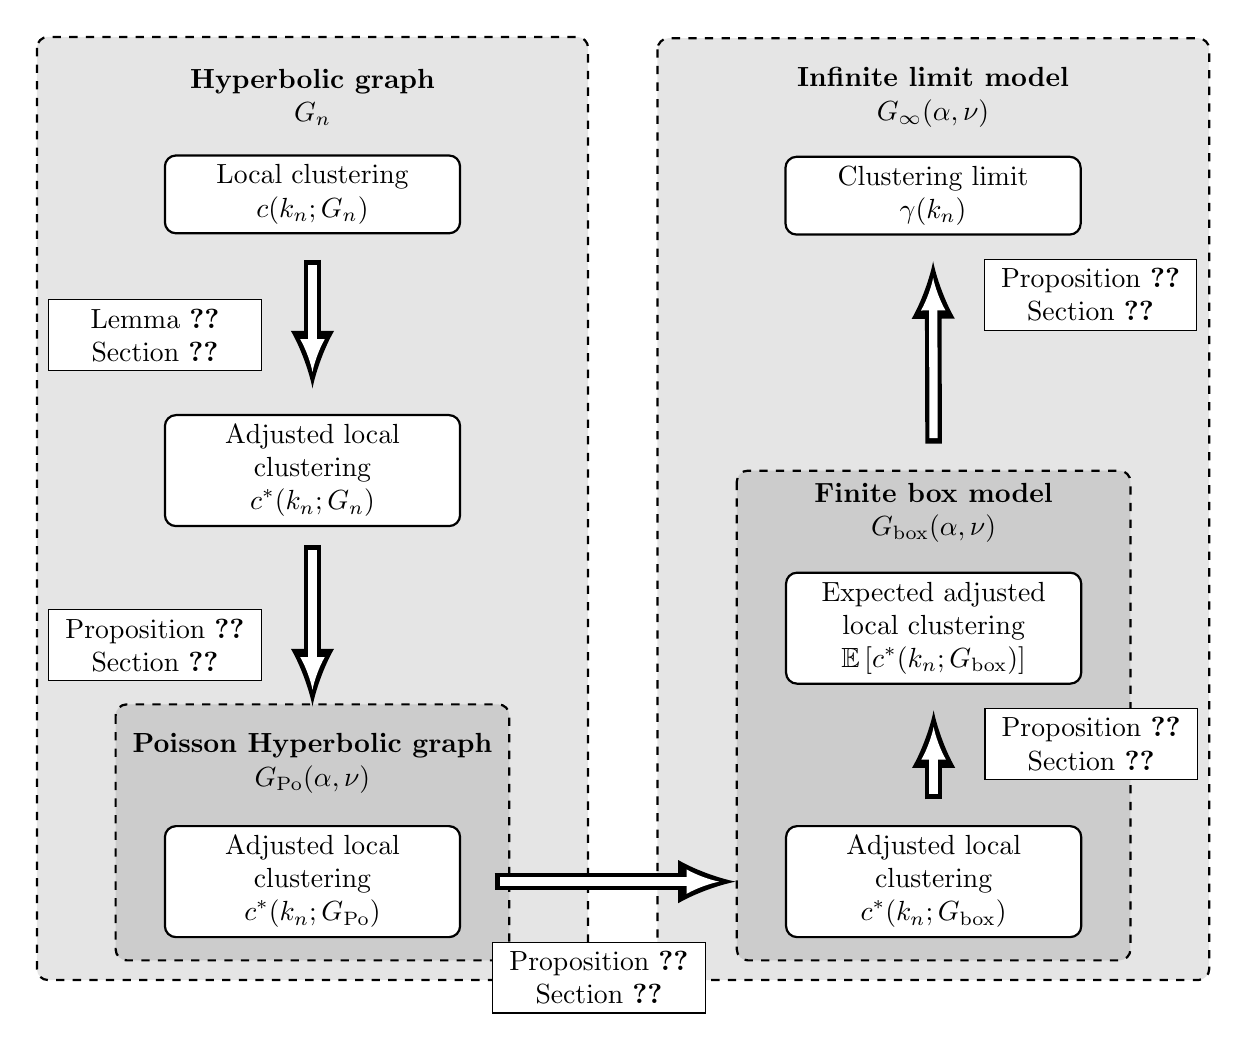
\begin{tikzpicture}

\pgfdeclarelayer{background}
\pgfdeclarelayer{foreground}
\pgfsetlayers{background,main,foreground}

\tikzstyle{block} = [draw, text centered, rounded corners, draw=black, thick, fill=white]
\tikzstyle{textblock} = [draw, text centered, draw=black, fill=white]

\tikzset{
  double arrow/.style args={#1 colored by #2 and #3}{
    -latex,line width=#1,#2, % first arrow
    postaction={draw,-latex,#3,line width=(#1)/2,
                shorten <=(#1)/3,shorten >=(#1)}, % second arrow
  }
}

\draw node (anchor) at (0,0) {};

%Hyperbolic graph: top left

\path (anchor)+(0,0) node (hyp_header) {\begin{minipage}[c]{10em}
	\begin{center}
		\textbf{Hyperbolic graph}\\
		$G_n$
	\end{center}
\end{minipage}};

\path (hyp_header.south)+(0,-0.75) node (c_hyp) [block] {\begin{minipage}[c]{10em}
	\begin{center}
	Local clustering\\
	$\displaystyle c(k_n;G_n)$
	\end{center}
\end{minipage}};






%Adjusted local clustering: middle left

\path (c_hyp.south)+(0,-3) node (c_ast_hyp) [block] {\begin{minipage}[c]{10em}
	\begin{center}
	Adjusted local clustering\\
	$\displaystyle c^\ast(k_n;G_n)$
	\end{center}
\end{minipage}};

\path (c_ast_hyp.north)+(-2,1) node (hyp_text) [textblock] {\begin{minipage}[c]{7em}
	\begin{center}
		Lemma \ref{lem:clustering_ast_H}\\
		Section~\ref{ssec:coupling_H_HP}
	\end{center}
\end{minipage}};

%Poisson Hyperbolic graph: middle left

%\path (c_hyp.south)+(0,-6) node (c_pois_hyp) [block] {\begin{minipage}[c]{12em}
%	\begin{center}
%	Local clustering\\
%	$\displaystyle c_{\widetilde{\H},n}(k_n)$
%	\end{center}
%\end{minipage}};



\path (c_ast_hyp.south)+(0,-3) node (pois_hyp_header) {\begin{minipage}[c]{13em}
	\begin{center}
		\textbf{Poisson Hyperbolic graph}\\
		$\GPo(\alpha,\nu)$
	\end{center}
\end{minipage}};

\path (pois_hyp_header.north)+(-2,1) node (pois_hyp_text) [textblock] {\begin{minipage}[c]{7em}
	\begin{center}
		Proposition \ref{prop:clustering_ast_H_Pois}\\
		Section~\ref{ssec:coupling_H_HP}
	\end{center}
\end{minipage}};





%Poisson Hyperbolic graph: bottom left

\path (pois_hyp_header.south)+(0,-1) node (c_ast_pois_hyp) [block] {\begin{minipage}[c]{10em}
	\begin{center}
	Adjusted local clustering\\
	$\displaystyle c^\ast(k_n; \GPo)$
	\end{center}
\end{minipage}};



%Infinite limit model: top right



\path (hyp_header.east)+(6,0) node (pois_header) {\begin{minipage}[c]{10em}
	\begin{center}
		\textbf{Infinite limit model}\\
		$\Ginf(\alpha, \nu)$
	\end{center}
\end{minipage}};

\path (pois_header)+(0,-1.25) node (c_infty) [block] {\begin{minipage}[c]{10em}
	\begin{center}
	Clustering limit\\
	$\displaystyle \gamma(k_n)$
	\end{center}
\end{minipage}};

\path (c_infty.south)+(2,-0.75) node (exp_c_pois_text) [textblock] {\begin{minipage}[c]{7em}
	\begin{center}
		Proposition \ref{prop:convergence_average_clustering_P_n}\\
		Section \ref{sec:clustering_Pn_to_P}
	\end{center}
\end{minipage}};




%Finite box model: bottom right

\path (c_ast_pois_hyp.east)+(6,0) node (c_ast_pois_n) [block] {\begin{minipage}[c]{10em}
	\begin{center}
	Adjusted local clustering\\
	$\displaystyle c^\ast(k_n; \Gbox)$
	\end{center}
\end{minipage}};

\path (c_ast_pois_n.south)+(-4.25,-0.5) node (c_ast_pois_n_text) [textblock] {\begin{minipage}[c]{7em}
	\begin{center}
		Proposition \ref{prop:couling_c_H_P}\\
		Section \ref{ssec:coupling_HP_ast_P}
	\end{center}
\end{minipage}};

\path (c_ast_pois_n.north)+(0,2.5) node (exp_c_pois_n) [block] {\begin{minipage}[c]{10em}
	\begin{center}
	Expected adjusted local clustering\\
	$\displaystyle \Exp{c^\ast(k_n; \Gbox)}$
	\end{center}
\end{minipage}};

\path (exp_c_pois_n.south)+(2,-0.75) node (exp_c_pois_n_text) [textblock] {\begin{minipage}[c]{7em}
	\begin{center}
		Proposition \ref{prop:concentration_local_clustering_P_n}\\
		Section \ref{sec:concentration_c_P_n}
	\end{center}
\end{minipage}};

\path (exp_c_pois_n.north)+(0,0.75) node (pois_n_header) {\begin{minipage}[c]{13em}
	\begin{center}
		\textbf{Finite box model}\\
		$\Gbox(\alpha, \nu)$
	\end{center}
\end{minipage}};








%Arrows

\path (c_hyp.south)+(0,-0.2) node (arrow_1l) {};
\path (c_ast_hyp.north)+(0,0.2) node (arrow_1r) {};

\draw [double arrow=6pt colored by black and white] (arrow_1l) -- (arrow_1r);

\path (c_ast_hyp.south)+(0,-0.1) node (arrow_2l) {};
\path (pois_hyp_header.north)+(0,0.1) node (arrow_2r) {};

\draw [double arrow=6pt colored by black and white] (arrow_2l) -- (arrow_2r);

\path (c_ast_pois_hyp.east)+(0.3,0) node (arrow_3l) {};
\path (c_ast_pois_n.west)+(-0.5,0) node (arrow_3r) {};

\draw [double arrow=6pt colored by black and white] (arrow_3l) -- (arrow_3r);

\path (c_ast_pois_n.north)+(0,0.2) node (arrow_4l) {};
\path (exp_c_pois_n.south)+(0,-0.2) node (arrow_4r) {};

\draw [double arrow=6pt colored by black and white] (arrow_4l) -- (arrow_4r);

\path (exp_c_pois_n.north)+(0,1.5) node (arrow_5l) {};
\path (c_infty.south)+(0,-0.2) node (arrow_5r) {};

\draw [double arrow=6pt colored by black and white] (arrow_5l) -- (arrow_5r);

\begin{pgfonlayer}{background}

\path (c_hyp)+(-3.5,2) node (hyp_a) {};
\path (c_ast_pois_hyp)+(3.5,-1.25) node (hyp_b) {};
\path[rounded corners, draw=black, dashed, thick, fill=black!10] (hyp_a) rectangle (hyp_b);

\path (pois_hyp_header)+(-2.5,0.75) node (pois_hyp_a) {};
\path (c_ast_pois_hyp)+(2.5,-1) node (pois_hyp_b) {};
\path[rounded corners, draw=black, dashed, thick, fill=black!20] (pois_hyp_a) rectangle (pois_hyp_b);

\path (c_infty)+(-3.5,2) node (pois_a) {};
\path (c_ast_pois_n)+(3.5,-1.25) node (pois_b) {};
\path[rounded corners, draw=black, dashed, thick, fill=black!10] (pois_a) rectangle (pois_b);

\path (exp_c_pois_n)+(-2.5,2) node (pois_n_a) {};
\path (c_ast_pois_n)+(2.5,-1) node (pois_n_b) {};
\path[rounded corners, draw=black, dashed, thick, fill=black!20] (pois_n_a) rectangle (pois_n_b);

\end{pgfonlayer}

\end{tikzpicture}

\caption{Overview of the proof strategy for Theorem \ref{thm:local_clustering_hyperbolic}.}
\label{fig:overview_proof}
\end{figure}


\subsection{Adjusted clustering and Poisson nodes in hyperbolic graphs}

Recall that the first step for the fixed $k$ case was to show that the transition from the hyperbolic random graph $G_{\H,n}$ to the Poisson version $\GPo$ did not influence clustering. Here we first make a transition from the local clustering function $c_{\H,n}(k)$ to the adjusted version $c^\ast(k; G_n)$. The following lemma justifies working with this modified version. The proof uses a concentration result for $\N_{\H,n}(k_n)$ and full details can be found in Section~\ref{ssec:coupling_H_HP}.

\begin{lemma}\label{lem:clustering_ast_H}
As $n \to \infty$,
\[
	\Exp{\left|c(k_n;G_n) - c^\ast(k_n;G_n)\right|} = \smallO{s(k_n)}.
\]
\end{lemma}

We then establish that the modified local clustering function in the hyperbolic model $G_{\H,n}(\alpha,\nu)$ behaves similarly to that in the Poisson version $G_{\HP, n}(\alpha,\nu)$. This is based on a standard coupling between a Binomial Point Process and Poisson Point Process.

\begin{proposition}\label{prop:clustering_ast_H_Pois}
As $n \to \infty$,
\[
	\Exp{\left|c^\ast(k_n;G_n) - c^\ast(k_n; \GPo)\right|} = \smallO{s(k_n)}.
\]
\end{proposition}
%\MS{I think we can drop the condition to be increasing here and below, also the $n^{1/3}$ should be removed.}

\subsection{Coupling of local clustering between $\GPo$ and $\Gbox$}

The next step is to show that the modified clustering is preserved under the coupling described in Section~\ref{ssec:coupling_H_P}. The proof can be found in Section~\ref{ssec:coupling_HP_ast_P}. This is one of the key technical challenges we face. 

To understand why, recall that the degree $k$ of a node is related to its height $y$, roughly speaking, by $k \approx \xi e^{y/2}$. Therefore, when $k$ is fixed we have that the heights of nodes with that degree are also fixed, in particular $y < R_n/4$ for large enough $n$. In addition, the main contribution of triangles would also come from nodes with heights $y^\prime < R_n/4$. This allowed us to use Lemma~\ref{lem:coupling_edges} and conclude that the triangles present in the graph $\GPo$ where exactly those present in $\Gbox$ and therefore the local clustering function was the same in both models. When $k_n \to \infty$ this is no longer true in general. For instance, suppose $k_n = n^{\frac{1-\varepsilon}{2\alpha + 1}}$, for some small $0 < \varepsilon < 1$. Then the relation $k_n \approx \xi e^{y_n/2}$ implies that $y_n \approx \frac{2(1-\varepsilon)}{2\alpha + 1}\log(n) - 2\log(\xi)$. Since
$R_n/4 = \frac{1}{2}\log(n) - \frac{1}{2}\log(\nu)$ we get that $R_n/4 = \smallO{y_n}$ for all $\alpha > (3 - 4\varepsilon)/2$ and hence $y_n > R_n/4$ for large enough $n$, violating the conditions of Lemma~\ref{lem:coupling_edges}. However, by carefully analyzing the difference between the adjusted local clustering function in both models we can still make the same conclusion. This is summarized in the following proposition whose proof is found in Section~\ref{ssec:coupling_HP_ast_P}.

\begin{proposition}[Coupling result for local clustering]\label{prop:couling_c_H_P}
As $n \to \infty$,
\[
	\Exp{\left|c^\ast(k_n; \GPo) - c^\ast(k_n; \Gbox)\right|} = \smallO{s(k_n)}.
\]
\end{proposition}

\TM{ Maybe we could replace these three with a statement on $|c(k_n;G_n) - c^\ast(k_n; \Gbox)|$, at least at this point of the paper. This is only the high level description and that is all we need for the ``final proof".}\PvdH{I would vote for keeping them split, since this allows us to clearly point to the main technical challenge we have to overcome to obtain the final result.}
These three results together imply that the difference between the local clustering function of the hyperbolic random graph and the modified local clustering function of the finite box graph converges to zero faster than the proposed scaling $\gamma(k_n)$ in Theorem [??]. Hence, to prove this theorem it is enough to prove it for $c^\ast(k; \Gbox)$. 

\subsection{From the finite to the infinite model}

To compute the limit of the modified local clustering function $c^\ast(k; \Gbox)$ in the finite graph $G_{\mathcal{P},n}(\alpha, \nu)$ we first prove in Section~\ref{sec:concentration_c_P_n} that it is concentrated around its expectation $\Exp{c^\ast(k_n; \Gbox)}$.

\TM{ ``concentration'' is a loaded term in probability. I am not sure this use of the word will not be counterintuitive to many. }\PvdH{I am not sure. Concentration generally refers to how much a random variable deviates from its expectation. This is exactly what this proposition tells us. I would therefore vote for keeping this terminology, although I would have no problem with replacing it with an other term if someone has a good suggestion.}

\begin{proposition}[Concentration for local clustering function in $G_{\mathcal{P},n}(\alpha, \nu)$]\label{prop:concentration_local_clustering_P_n}
As $n \to \infty$,
\[
	\Exp{\left|c^\ast(k_n; \Gbox) - \Exp{c^\ast(k_n; \Gbox)}\right|} = \smallO{s(k_n)}.
\]
\end{proposition}

This result is another one of the technical challenges we face when considering $k_n \to \infty$. For the proof, we first identify the specific range of heights that give the main contribution to the triangle count, showing that the triangles coming from nodes with heights outside this range is of smaller order. Then we prove a concentration result for the main term, by carefully analyzing the joint neighborhoods of two nodes whose heights fall into the identified range. The full details are found in Section~\ref{sec:concentration_c_P_n}.

Assuming this concentration result, we are left with the task to compute the limit of $\Exp{c^\ast(k_n; \Gbox)}$ as $n \to \infty$ and show that it is equivalent to $\gamma(k_n)$. To accomplish this we move to the infinite limit model $\Ginf$ and show that the difference between the expected value of $c^\ast(k;\Gbox)$ and $\gamma(k_n)$ goes to zero faster than the proposed scaling in Theorem \ref{thm:local_clustering_hyperbolic}.

\begin{proposition}[Transition to the infinite limit model]\label{prop:convergence_average_clustering_P_n}
As $n \to \infty$,
\[
	\left|\Exp{c^\ast(k_n; \Gbox)} - \gamma(k_n)\right| = \smallO{s(k_n)}.
\]
\end{proposition}

\TM{ This is only for $c(k)$. Should we not also mean $c$? }\PvdH{I do not think so. We can prove everything for $c$ once we have the result for $c(k_n)$.}

Recall that for the finite box model the left and right boundaries of $\Rcal_n$ where identified, so that graph $\Gbox$ contains some additional edge with respect to the induced subgraph of $\Ginf$ on $\Rcal_n$. The prove of Proposition~\ref{prop:convergence_average_clustering_P_n} therefore relies on analyzing the number of triangles coming from these additional edges and showing that their contribution to the local clustering function are of negligible order, see Section~\ref{sec:clustering_Pn_to_P}. 

\begin{remark}[Notations different graphs]
We will use the subscripts $n$, $\Po$, $\text{box}$ and $\infty$ to identify properties of, respectively, the KPKVB mode $G_n$, the Poisson version $\GPo$, the finite box model $\Gbox$ and the infinite model $\Ginf$. For example $N_{\Po}(k)$ denotes number of nodes with degree $k$ in $\GPo$ and $\rho_{\text{box}}(y,k) = \Prob{\Po(\mu(\BallPo{y})) = k}$, i.e. the degree distribution of a typical point in $\Gbox$.
\end{remark}

\subsection{Proof of the main results}\label{ssec:proof_main_result_diverging_k}

We are now ready to prove Theorem~\ref{thm:mainktoinfty}, using the propositions stated in the previous sections.

\begin{proof}[Proof of Theorem~\ref{thm:mainktoinfty}]
%By applying Proposition~\ref{prop:convergence_average_clustering_P_n}, Proposition~\ref{prop:convergence_average_clustering_P_n} and Theorem~\ref{thm:asymptotics_average_clustering_P} we get
%\begin{align*}
%	&\hspace{-30pt}\Exp{\left|\frac{c^\ast(k_n; \Gbox)}{C_{\alpha,\nu}\gamma(k_n)} - 1\right|}\\
%	&\le \frac{\Exp{\left|c^\ast(k_n; \Gbox) - \Exp{}c^\ast(k_n; \Gbox)\right|}}{C_{\alpha,\nu}\gamma(k_n)}
%		+ \frac{\left|\Exp{c^\ast(k_n; \Gbox)} - \gamma(k_n)\right|}{C_{\alpha,\nu}\gamma(k_n)}
%		+ \left|\frac{c_{\infty}(k_n)}{C_{\alpha,\nu}\gamma(k_n)} - 1\right| \\
%	&= \smallO{1}.
%\end{align*}
First of all, due to cancellation of equal terms we can rewrite
\begin{align*}
    c(k_n;G_n)-\gamma(k_n) =& c(k_n;G_n)-c^\ast(k_n;G_n)+c^\ast(k_n;G_n)-c^\ast(k_n; \GPo)+c^\ast(k_n; \GPo)-c^\ast(k_n; \Gbox) \\
    &+c^\ast(k_n; \Gbox)-\E c^\ast(k_n; \Gbox)+\E c^\ast(k_n; \Gbox)-\gamma(k_n)
\end{align*}
Then, we take absolute values and apply the triangle inequality. By monotonicity of expectation, we can apply it to both sides and obtain
\begin{align*}
    \E[|c(k_n;G_n)-\gamma(k_n)|] \leq & \E[|c(k_n;G_n)-c^\ast(k_n;G_n)|]+\E[|c^\ast(k_n;G_n)-c^\ast(k_n; \GPo)|]\\&+\E[|c^\ast(k_n; \GPo)-c^\ast(k_n; \Gbox)|] 
    +\E[|c^\ast(k_n; \Gbox)-\E c^\ast(k_n; \Gbox)|]\\&+\E[|\E c^\ast(k_n; \Gbox)-\gamma(k_n)|]
\end{align*}
At this point, the lemmas and propositions presented above in this section can be applied in order to show that all summands are $\smallO{\gamma(k_n)}$: Lemma~\ref{lem:clustering_ast_H} for the transition to the modified clustering function in the first term, Proposition~\ref{prop:clustering_ast_H_Pois} for the Poissonization in the disk in the second term, Proposition~\ref{prop:couling_c_H_P} for the coupling from the disk to the finite box model in the third term, Proposition~\ref{prop:concentration_local_clustering_P_n} for the concentration in the fourth term and finally Proposition~\ref{prop:convergence_average_clustering_P_n} for the transition to the infinite limit model. 
%where we also used that $c(k_n;\Ginf) = \gamma(k_n)$ as obtained at the end of Section~\ref{sec:asymptotics_average_clustering_ast_P}.
%\TM{ Maybe we can have a more clear reference? Now, at this place in the paper this proof feels a bit like cheating since there are almost no details given. } \PvdH{I completely agree. I think that once the results for fixed $k$ have been included we can include a specific statement at the end of Section~\ref{sec:asymptotics_average_clustering_ast_P} we can refer to.} 
All of this together yields that:
\begin{align*}
    \E[|c(k_n;G_n)-\gamma(k_n)|] = \smallO{s(k_n)} = \smallO{\gamma(k_n)},
\end{align*}
%\TM{ Last equality seems to rely on Thm 1.3, which is not yet proven at this point. }\PvdH{We can fix this by proving the scaling of $c_\infty(k)$ in Section~\ref{sec:asymptotics_average_clustering_ast_P}.}
i.e. the statement of the theorem.
%\[
%	\Exp{\left|\frac{c^\ast(k_n; \Gbox)}{C_{\alpha,\nu}\gamma(k_n)} - 1\right|}
%	\le \left|\frac{c_{\infty}(k_n)}{C_{\alpha,\nu}\gamma(k_n)} - 1\right| 
%	+ \frac{\Exp{\left|c^\ast(k_n; \Gbox) - \gamma(k_n)\right|}}{C_{\alpha,\nu}\gamma(k_n)} = \smallO{1}.
%\]

%Combining this with Proposition~\ref{prop:couling_c_H_P} yields
%\[
%	\Exp{\left|\frac{c^\ast(k_n;G_n)}{C_{\alpha,\nu}\gamma(k_n)} - 1\right|}
%	\le \Exp{\left|\frac{c^\ast(k_n; \Gbox)}{C_{\alpha,\nu}\gamma(k_n)} - 1\right|} 
%	+ \frac{\Exp{\left|c^\ast(k_n;G_n) - c^\ast(k_n; \Gbox)\right|}}{C_{\alpha,\nu}\gamma(k_n)} = \smallO{1}.
%\]
%and the result then follows by applying Lemma~\ref{lem:clustering_ast_H}. 
\end{proof}



\section{From $\Gbox$ to $\Ginf$ (Proving Proposition \ref{prop:convergence_average_clustering_P_n})}\label{sec:clustering_Pn_to_P}

In this section we shall relate the clustering in the finite box model $\Gbox$ to that of the infinite model. The main goal is to prove Proposition~\ref{prop:convergence_average_clustering_P_n} which states that
\[
	\left|\Exp{c^\ast(k_n; \Gbox)} - \gamma(k_n)\right| = \smallO{s(k_n)}.
\] 

Recall that $\Gbox$ is obtained by restricting the Poisson Point Process $\PPP$ to the box $\Rcal = (-I_n, I_n] \times (0, R_n]$, with $I_n = \frac{\pi}{2} e^{R_n/2}$ and connecting two points $p_1, p_2 \in \Rcal$ if $|x_1 - x_2|_{\pi e^{R_n/2}} \le e^{(y_1 + y_2)/2}$. We also recall that by definition of the norm $|.|_{\pi e^{R_n/2}}$ the left and right boundaries of $\Rcal$ are identified. See Section~\ref{ssec:finite_model} for more details. Due to this identification of the boundaries some triples of nodes that form triangles in the finite box model do not form a triangle in the infinite model. Therefore, to establish the required result we need to compute the asymptotic difference between triangle counts in both models.


%\TM{ This last bit of the sentence is already contained in the fact we us $|.|_{\pi e^{R_n/2}}$. To me it does not add anything, except possibly confusion. } \PvdH{I have updated this and just added a reminder of this.}

%In this section we shall compute the asymptotic difference between triangle counts in the finite box and infinite model. First we recall the definition of $\Kcal_{C}(k_n)$
%\[
%	\Kcal_C(k_n) = \left\{y \in \R_+ : \frac{k_n - C \sqrt{k_n \log(k_n)}}{\xi} \le e^{\frac{y}{2}}
%	\le \frac{k_n + C \sqrt{k_n \log(k_n)}}{\xi} \right\},	
%\]
%\TM{ Typo : $p\in\R$. Do you mean $\Rcal$? Or maybe 
%$\R \times \R^+$? Still not sure that max and min in defn add anything. } \PvdH{It was a typo and is corrected. I have removed the max and min.}
%with
%\[
%	\kappa_n := \begin{cases}
%		\log(n) &\mbox{if } k_n = \bigT{1},\\
%		\sqrt{k_n \log(k_n)} &\mbox{else.}
%	\end{cases}
%\]
%\TM{ Same issue as before. }
%In addition we note that the function $\phi_n(y)$ in Lemma~\ref{lem:average_degree_P_n} satisfies
%\[
%	\phi_n(y) = \bigT{e^{-(\alpha - \frac{1}{2})(R_n - y)}},
%\]
%as $R_n - y \to \infty$. Since $e^{y/2} = \bigT{k_n} = \smallO{e^{R_n}}$ as $n \to \infty$, uniformly on $\Kcal_C(k_n)$, it follows that $\phi_n(y) = \bigT{k_n^{2\alpha - 1} n^{-(2\alpha - 1)}}$, uniformly on $\Kcal_C$. This yields the following useful corollary to Lemma~\ref{lem:average_degree_P_n}.
%
%\begin{corollary}\label{cor:average_degree_P_n_K}
%Let $\alpha > \frac{1}{2}$, $C > 0$. Then, for all $y \in \Kcal_{C}(k_n)$,
%\[
%	\mu(\BallPon{y}) = \mu(\BallPo{y})\left(1 - \bigT{k_n^{2\alpha - 1} n^{-(2\alpha - 1)}}\right).
%\]
%\TM{ I don't follow. Spell it out. }\PvdH{I added additional explanation above. Please see if this solves the confusion.}
%
%\end{corollary}




%We now turn to the task of calculating the expected number of triangles of a node at height $y$, for both the infinite model and the finite box model. 
For any $p \in \R \times \R_+$ we define for the finite box model,
\[
	T_{\text{box}}(p) = \sum^{\ne}_{p_1, p_2 \in \Pcal_n \setminus p} T_{\text{box}}(p,p_1,p_2)
\]
where the sum is over all distinct pairs in $\Pcal_n \setminus p$ and
\[
	T_{\text{box}}(p,p_1,p_2) = \ind{p_1 \in \BallPon{p}}\ind{p_2 \in \BallPon{p}}\ind{p_2 \in \BallPon{p_1}}.
\]
Similarly, for the infinite model we define
\[
	T_\infty(y) = \sum_{p_1, p_2 \in \Pcal \setminus \{0,y\}}^{\ne} T_\infty(y,p_1,p_2),
\]
where
\[
	T_{\infty}(y,p_1,p_2) = \ind{p_1 \in \BallPo{y}}\ind{p_2 \in \BallPo{y}}\ind{p_2 \in \BallPo{p_1}}.
\]
We will first relate $\gamma(k_n)$ and $\Exp{c^\ast(k_n; \Gbox)}$ using $T_\infty(y)$ and $T_{\text{box}}(y)$. Recall the definition of $\Kcal_{C}(k_n)$
\[
	\Kcal_C(k_n) = \left\{y \in \R_+ : \frac{k_n - C \sqrt{k_n \log(k_n)}}{\xi} \le e^{\frac{y}{2}}
	\le \frac{k_n + C \sqrt{k_n \log(k_n)}}{\xi} \right\},	
\]

\begin{lemma}
Let $\gamma(k_n)$ be defined as in~\eqref{eq:gammakint}. Then as $n \to \infty$
\begin{equation}\label{eq:alt_gamma_kn}
	\gamma(k_n) = (1+\smallO{1})\frac{1}{k_n^2 p_{k_n}} \int_{\Kcal_{C}(k_n)} \Exp{T_\infty(y)} \rho(y,k) 
				\alpha e^{-\alpha y} \dd y. 
\end{equation}
Moreover,
\begin{equation}\label{eq:alt_c_ast_kn}
	\Exp{c^\ast(k_n;\Gbox)} = (1 + \smallO{1}) \frac{1}{k_n^2 p_{k_n}} \int_{\Kcal_{C}(k_n)} \Exp{T_{\text{box}}(y)}
		\rho(y,k_n) \alpha e^{-\alpha y} \dd y
\end{equation}
as $n \to \infty$,
\end{lemma}

\begin{proof}
Recall that 
\[
	P(y) = \Exp{\ind{u_1 \in \BallPo{u_2}}},
\]
where $u_1$ and $u_2$ are independent and distributed according to the probability density \\$\Mu{\BallPo{y}}^{-1} \ind{u_i \in \BallPo{y}} f(x_i, y_i)$. It then follows from the Campbell-Mecke formula that
\begin{align*}
	\Exp{T_\infty(y)} &= \int \ind{p_1 \in \BallPo{y}}\ind{p_2 \in \BallPo{y}}
		\ind{p_2 \in \BallPo{p_1}} f(x_1,y_1) f(x_2,y_2) \dd x_1 \dd x_2 \dd y_1 \dd y_2\\
	&= \Mu{\BallPo{y}}^2 P(y).
\end{align*}
It then follows that,
\begin{align*}
	\gamma(k_n) &= \frac{1}{p_{k_n}} \cdot \int_0^\infty P(y) \rho(y,k) \alpha e^{-\alpha y} \dd y \\
	&= \frac{1}{p_{k_n}} \int_0^\infty \Exp{T_\infty(y)} \Mu{\BallPo{y}}^{-2} \rho(y,k) 
		\alpha e^{-\alpha y_0} \dd y_0\\
	&= (1+ \smallO{1}) \frac{1}{k_n^2 p_{k_n}} \int_0^\infty \Exp{T_\infty(y)} \rho(y,k) \alpha e^{-\alpha y} \dd y_0,
\end{align*}
where the last line is due to a concentration of heights argument.

For~\eqref{eq:alt_c_ast_kn} we recall that
\[
	c^\ast(k_n; \Gbox) = \frac{1}{\Exp{\Nbox(k_n)}} \sum_{p \in \Pcal} c_{\text{box}}(p)\ind{\Dbox(p) = k_n},
\]
where $c_{\text{box}}(p)$ can be expressed as
\[
	c_{\text{box}}(p) = \frac{1}{\binom{\Dbox(p)}{2}} \sum_{p_1, p_2 \in \Pcal \setminus p}^{\ne} T_{\text{box}}(p,p_1,p_2)
	= \frac{T_{\text{box}}(p)}{\binom{\Dbox(p)}{2}}.
\]
By the Campbell-Mecje formula
\begin{align*}
	\Exp{c^\ast(k_n; \Gbox)} 
	&= \frac{1}{\Exp{\Nbox(k_n)}} \int_{\Rcal} \Exp{c_{\text{box}}(p)\ind{\Dbox(p) = k_n}} f(x,y) \dd x \dd y\\
	&= \frac{1}{\Exp{\Nbox(k_n)}} \int_{\Rcal} \CExp{c_{\text{box}}(p)}{\Dbox(p) = k_n}\rho_{\text{box}}(p,k_n) 
		f(x,y) \dd x \dd y\\
	&= (1+\smallO{1})\frac{n}{\Exp{\Nbox(k_n)}} \int_{\Kcal_C(k_n)} \CExp{c_{\text{box}}(y)}{\Dbox(y) = k_n}
		\rho(y,k_n) \alpha e^{-\alpha y} \dd y,
\end{align*}
where the last line follows from a concentration of heights argument, for which we used that $\CExp{c_{\text{box}}(y)}{\Dbox(y) = k_n} \le 1$. To analyze the conditional expectation we observe that, similar to the analysis of $\gamma(k_n)$, conditioned on their being $k_n$ points in $\BallPon{y}$, each points $u_i = (x_i,y_i)$ is independently distributed according to the probability density $\Mu{\BallPon{y}}^{-1} \ind{u_i \in \BallPon{y}} f(x_i,y_i)$. Therefore,
\begin{align*}
	\CExp{c_{\text{box}}(y)}{\Dbox(y) = k_n}
	&= \binom{k_n}{2}^{-1} \Exp{\sum_{1 \le i < j \le k_n} \ind{u_i \in \BallPon{u_j}}} \\
	&= \Exp{u_1 \in \BallPon{u_2}} \\
	&= \Mu{\BallPon{y}}^{-2} \iint T_{\text{box}}(y,p_1,p_2) f(x_1,y_1) f(x_2,y_2) 
		\dd x_1 \dd y_1 \dd x_2 \dd y_2\\
	&= \Mu{\BallPon{y}}^{-2} \Exp{T_{\text{box}}(y)}.
\end{align*}
and thus, by applying a concentration of heights argument on $\Mu{\BallPon{y}}^{-2}$,
\[
	\Exp{c^\ast(k_n; \Gbox)} = (1 + \smallO{1}) \frac{n \Mu{\BallPon{2\log(k_n/\xi)}}^{-2}}{\Exp{\Nbox(k_n)}} \int_{\Kcal_C(k_n)} \Exp{T_{\text{box}}(y)} \rho(y,k_n) \alpha e^{-\alpha y} \dd y.
\]
To finish the argument, we first note that $\Mu{\BallPon{2\log(k_n/\xi)}}^{-2} = (1+\smallO{1})k_n^2$, while
\[
	\Exp{N_{\text{box}}(k_n)} = \int_{\Rcal} \rho_{\text{box}}(y,k_n) f(x,y) \dd x \dd y,
\]
so that by a concentration of heights argument,
\[
	\Exp{N_{\text{box}}(k_n)} = (1+o(1)) n \int_{0}^\infty \rho(y,k_n) \alpha e^{-\alpha y} \dd y 
	= (1+\smallO{1}) n p_{k_n}.
\]
We therefore conclude that
\[
	\Exp{c^\ast(k_n; \Gbox)} = (1 + \smallO{1}) \frac{1}{k_n^2 p_{k_n}} \int_{\Kcal_C(k_n)} 
		\Exp{T_{\text{box}}(y)} \rho(y,k_n) \alpha e^{-\alpha y} \dd y.
\]


%Next recall the definition of $\Kcal_{C}(k_n)$, see~\eqref{eq:def_K_C_set}, and note that for all $y_0 \in \Kcal_{C}(k_n)$, $\mu(y) = (1+\smallO{1})k_n$. Then Lemma~\ref{lem:concentration_argument} implies that, as $n \to \infty$,
%\begin{align*}
%	&\hspace{-30pt} \int_0^\infty \Exp{T_\infty(y_0)} \left(\frac{\mu(y)^2}{2}\right)^{-1} \rho(y_0,k) 
%		\alpha e^{-\alpha y_0} \dd y_0\\
%	&= (1+ \smallO{1}) \binom{k_n}{2}^{-1} \int_0^\infty \Exp{T_\infty(y_0)} \rho(y_0,k) \alpha e^{-\alpha y_0} \dd y_0,
%\end{align*}
%which finishes the proof.
\end{proof}


%
%
%For the finite box model we have, by the Campbell-Mecke formula,
%\begin{align*}
%	\Exp{c^\ast(k_n, \Gbox)}
%	&= \frac{1}{\binom{k_n}{2}\Exp{\Nbox(k_n)}} \int_{\Rcal} \Exp{T_{\text{box}}(p) \ind{\text{deg}(p) = k_n}} f(x,y) 
%		\dd x \dd y\\
%	&= \frac{n}{\binom{k_n}{2}N_{\Gbox}(k_n)} \int_0^{R} \CExp{T_{\text{box}}(y_0)}{\text{deg}(y_0) = k_n} 
%		\rho_{\text{box}}(y,k_n) \alpha e^{-\alpha y_0} \dd y_0,
%\end{align*}
%where the last line follows since the Poisson point process is invariant in $x$ and by slightly abusing notation $T_{\text{box}}(y_0) = T_{\text{box}}(0,y_0)$. Next we note that 
%\[
%	\Exp{N_{\text{box}}(k_n)} = \int_{\Rcal} \rho_{\text{box}}(y,k_n) f(x,y) \dd x \dd y,
%\]
%so that by a concentration of heights argument, see Corollary~\ref{cor:concentration_heights_asymptotics_n},
%\[
%	\Exp{N_{\text{box}}(k_n)} = (1+o(1)) \alpha n \int_{0}^\infty \rho(y,k_n) e^{-\alpha y} \dd y 
%	= (1+\smallO{1}) n p_{k_n}.
%\]
%Since $\Exp{T_{\text{box}}(y_0)\ind{\text{deg}(y_0) = k_n}} \le \binom{k_n}{2}$, and Another concentration of heights argument yields
%\[
%	\int_0^{R} \Exp{T_{\text{box}}(y_0)} \rho_{\text{box}}(y_0,k_n) \alpha e^{-\alpha y_0} \dd y_0
%	= (1 + \smallO{1}) \int_{\Kcal_{C}(k_n)} \Exp{T_{\text{box}}(y_0)} \rho(y_0,k_n) \alpha e^{-\alpha y_0} \dd y_0
%\]
%and hence
%\begin{equation}\label{eq:approx_c_ast_Gbox}
%	c^\ast(k_n, \Gbox)  = (1 + \smallO{1})\frac{1}{p_{k_n}} \int_{\Kcal_{C}(k_n)} \binom{k_n}{2}^{-1} \Exp{T_{\text{box}}(y_0)} \rho(y_0,k_n) \alpha e^{-\alpha y_0} \dd y_0.
%\end{equation}

Comparing~\eqref{eq:alt_gamma_kn} and~\eqref{eq:alt_c_ast_kn}, we conclude that to prove Proposition~\ref{prop:convergence_average_clustering_P_n} it is enough to show that
\begin{equation}\label{eq:triangle_diff_main_term}
	 \left|\int_{\Kcal_{C}(k_n)} \Exp{T_{\text{box}}(y) - T_\infty(y)}
	\rho(y,k) \alpha e^{-\alpha y} \, d y \right|
	= \smallO{s(k_n)p_{k_n}k_n^2},
\end{equation}
which means we have to compute the expected difference in triangles between both models.


%it follows that
%\[
%	\Exp{T_{\text{box}}(p_0)} = \frac{1}{2}\iint_{\Rcal^2} T_{\text{box}}(p_0,p_1,p_2)
%	f(x_1,y_1) f(x_1,y_1) \, dx_1 \, dx_2 \, dy_1 \, dy_2,
%\]
%
%\TM{ $p$ is supposed to be $p_0$ I assume. }\PvdH{Indeed. It has been corrected.}

\subsection{Comparing triangles between $\Ginf$ and $\Gbox$}

To analyze $T_{\text{box}}(y_0) - T_\infty(y_0)$ we first reiterate that the difference between the indicator $\ind{p_1 \in \BallPon{p}}$ in the finite box model and $\ind{p_1 \in \BallPo{p}}$ is that in $\Gbox$ we identified the boundaries of the interval $[-\frac{\pi}{2}e^{R_n/2}, \frac{\pi}{2} e^{R_n/2}]$ and we stop at height $y = R_n$. This induces a difference in triangle counts between both models. 
To see this, note that for any $p = (x,y)$ with $0 \le y \le R_n$ we have that $\BallPon{p} = \BallPo{p} \cap \Rcal$. This means that if $p^\prime, p_2 \in \BallPon{p}$ and $p_2 \in \BallPo{p^\prime} \cap \Rcal$ then $p_2 \in \BallPon{p} \cap \BallPon{p^\prime}$ and hence $(p,p^\prime,p_2)$ form a triangle both in $\Gbox$ and $\Ginf$. However, it could happen that there are points in the intersection $\BallPon{p} \cap \BallPon{p^\prime}$ that are not in $\BallPo{p} \cap \BallPo{p^\prime}$. Let us denote this region by $\mathcal{T}(p \Delta p^\prime)$, see Figure~\ref{fig:comparing_triangles_diff_intersections} for an example of this region. Then, any $p_2 \in \mathcal{T}_{\Pcal \Delta \Pcal_n}(p,p^\prime)$ creates a triangle with $p$ and $p^\prime$ in $\Gbox$ that is not present in $\Ginf$. Finally, any point $p_2 \in \BallPo{p} \cap \BallPo{p6\prime}$ with height $y_2 > R$ creates a triangle with $p, p^\prime$ in $\Ginf$ but not in $\Gbox$.

Let us now define the following triangle count function
\[
	\widetilde{T}_{\text{box}}(p_0) = \sum_{(p_1, p_2) \in \Pcal \setminus p_0}^{\ne} 
		\widetilde{T}_{\text{box}}(p_0,p_1,p_2).
\]
where
\[
	\widetilde{T}_{\text{box}}(p_0,p_1,p_2) = \ind{p_1 \in \BallPon{p}}\ind{p_2 \in \BallPon{p}}\ind{p_2 \in \BallPo{p_1} \cap \Rcal}.
\]
Then $\widetilde{T}_{\text{box}}(p_0)$ only counts those triangles attached to $p_0$ that exist in both $\Gbox$ and $\Ginf$ and thus, by definition of the region $\mathcal{T}(p_0,p_1)$,
\[
	T_{\text{box}}(p_0) - \widetilde{T}_{\text{box}}(p_0)
	= \sum_{p_1, p_2 \in \Pcal }^{\ne} \ind{p_1 \in \BallPon{p_0}} 
			\ind{p_2 \in \mathcal{T}(p_0, p_1)}.
\]
%Thus, $\widetilde{T}_{\text{box}}(p_0)$ only count those triangles $(p_0,p_1,p_2)$ that also exist in $\Ginf$.
%Observe that the difference between $\widetilde{T}_{\text{box}}(p_0)$ and $T_{\text{box}}(p_0)$ is in the last indicator in $\widetilde{T}_{\text{box}}(p_0,p_1,p_2)$.  counts those points $p_2$ in the box $\Rcal$ that are in the neighborhood $\BallPo{p_1}$ of $p_1$ in the infinite model. Thus, $\widetilde{T}_{\text{box}}(p_0)$ only count those triangles $(p_0,p_1,p_2)$ that also exist in $\Ginf$.

  

The next result, which is crucial for the proof of Proposition~\ref{prop:convergence_average_clustering_P_n}, computes the expected measure of $\mathcal{T}_{\Pcal \Delta \Pcal_n}(p,p^\prime)$ with respect to $p^\prime$. 

\begin{lemma}\label{lem:clustering_error_T_term}
Let $p_0 = (0,y)$ with $y \in \Kcal_{C}(k_n)$. Then as $n \to \infty$,
\[
	\Exp{\left|T_{\text{box}}(p_0) - \widetilde{T}_{\text{box}}(p_0)\right|}
	= y \, \bigO{n^{-(2\alpha - 1)}} + e^{y}\,\bigO{n^{-(4\alpha-2)}}.
\]
%\[
%	\int_{\Rcal} \mu\left(\mathcal{T}_{\Pcal \Delta \Pcal_n}(p_0,p_1)\right) f(x_1,y_1) 
%	\dd x_1 \dd y_1 = \bigO{y n^{-(2\alpha - 1)} + n^{-(2\alpha-1)} e^{y}}
%\]
\end{lemma}

The proof of the lemma is not difficult but cumbersome, since it involves computing many different integrals. We postpone this proof till the end of this section and proceed with the main goal, proving Proposition~\ref{prop:convergence_average_clustering_P_n}. 

First we state a small lemma about the scaling of $s(k_n)$ that will be very useful.  

\begin{lemma}\label{lem:scaling_s_alpha}
Let $s(k_n)$ be as defined in \eqref{eq:def_scaling_function}. Then for any $k_n = \smallO{n^{\frac{1}{2\alpha + 1}}}$, as $n \to \infty$,
\[
	n^{-(2\alpha - 1)} = \smallO{s(k_n)}.
\]
\end{lemma}

\begin{proof}
First let $\frac{1}{2} < \alpha < \frac{3}{4}$. Then
\[
	n^{-(2\alpha - 1)}s(k_n)^{-1} = n^{-(2\alpha -1)}k_n^{4\alpha - 2}
	= \smallO{n^{-(2\alpha - 1) + \frac{4\alpha - 2}{2\alpha + 1}}} 
	= \smallO{n^{-\frac{4\alpha^2 - 4\alpha + 1}{2\alpha + 1}}}
	= \smallO{1},
\]
since $4\alpha^2 - 4\alpha + 1 > 0$ for all $\alpha > \frac{1}{2}$. Similarly, for $\alpha \ge \frac{3}{4}$ we have
that $4\alpha^2 > 2$ and hence,
\[
	n^{-(2\alpha - 1)} s_{\alpha}(k_n) = \smallO{n^{-(2\alpha - 1)} k_n} = \smallO{n^{-\frac{4\alpha^2 - 2}{2\alpha + 1}}}
	= \smallO{1}.
\]
\end{proof}

We now proceed with proving the main result of this section.

\begin{proof}[Proof of Proposition~\ref{prop:convergence_average_clustering_P_n}]
Let us write $\Rcal^\prime := \R \times \R_+ \setminus \Rcal$ and let $p_0 = (0,y)$ denote the typical point. Next we recall that it is enough to show~\eqref{eq:triangle_diff_main_term}, so that in particular we have that $y \in \Kcal_{C}(k_n)$.

Now
\begin{align*}
	\left|T_{\text{box}}(p_0) - T_{\infty}(p_0)\right| 
	&= \left|T_{\text{box}}(p_0) - \widetilde{T}_{\text{box}}(p_0)\right| 
		+ \sum_{p_1, p_2 \in \Pcal \cap \Rcal^\prime}^{\ne} T_{\infty}(p_0,p_1,p_2),
\end{align*}
so that by the Campbell-Mecke formula
\begin{align*}
	\left|\Exp{T_{\text{box}}(p_0) - T_{\infty}(p_0)}\right|
	&\le \Exp{\left|T_{\text{box}}(p_0) - \widetilde{T}_{\text{box}}(p_0)\right|}\\
	&\hspace{10pt}+ \int_{\Rcal^\prime}\int_{\Rcal^\prime} T_{\infty}(p_0,p_1,p_2) f(x_1,y_1) f(x_2,y_2)
		\dd x_2 \dd y_2 \dd x_1 \dd y_1. 
\end{align*}

\TM{ in the 1st integral we could have restricted to the ball of $p$, and possibly saved a lot. Does that not help? }\PvdH{the first integral is taken care of by another Lemma so it does not matter I think.}
The part is taken care of by Lemma~\ref{lem:clustering_error_T_term}. For the other integral we have
\begin{align*}
	&\hspace{-30pt}\iint_{\Rcal^\prime} T_{\infty}(p_0,p_1,p_2) f(x_1,y_1) f(x_2,y_2)
		\dd x_2 \dd y_2 \dd x_1 \dd y_1\\
	&\le \left(\int_{\Rcal^\prime} \ind{p_1 \in \BallPo{p_0}} f(x_1,y_1) \dd x_1 \dd y_1\right)^2
		= \bigO{\left(e^{y/2} \int_{R_n}^\infty e^{-(\alpha - \frac{1}{2})y_1} \dd y_1\right)^2}\\
	&= \bigO{e^{y} e^{-(2\alpha-1)R_n}} = \bigO{e^y n^{-(4\alpha - 2)}}.
\end{align*}
%\TM{ Typo : $f_{\mu, \nu}$? Also give more details how line 3 follows. }
We thus we conclude, using Lemma~\ref{lem:clustering_error_T_term}, that,
\begin{equation}\label{eq:triangle_count_diff_scaling}
	\left|\Exp{T_{\text{box}}(p_0) - T_{\infty}(p_0)}\right| = \bigO{y n^{-(2\alpha - 1)} + n^{-(4\alpha-2)} e^{y}}.
\end{equation}
Therefore, since $y = \bigO{\log(k_n)}$ on $\Kcal_C(k_n)$, 
\begin{align*}
	&\hspace{-30pt}\int_{\Kcal_{C}(k_n)} \rho(y,k_n) \left|\Exp{T_{\text{box}}(p_0) - T_{\infty}(p_0)}\right| 
		e^{-\alpha y_0} \dd y_0\\
	&= \bigO{1} \left(\log(k_n) n^{-(2\alpha - 1)} + k_n^2 n^{-(4\alpha - 2)} \right) 
		\int_{0}^\infty \rho(y_0,k_n) e^{-\alpha y_0} \dd y_0\\
	&= \bigO{1} \left(\log(k_n) n^{-(2\alpha - 1)} + k_n^2 n^{-(4\alpha - 2)} \right) p_{k_n} = \smallO{s(k_n) p_{k_n} k_n^2},
\end{align*}
%\TM{ Typo : $e^{-\alpha}$ }
where the last part follows from Lemma~\ref{lem:scaling_s_alpha} and the fact that $s(k_n)^2 = \smallO{s(k_n)}$. This establishes~\eqref{eq:triangle_diff_main_term} and hence finishes the proof.
%
% \TM{ Also justify penultimate step! }\PvdH{What do you mean?}
%To finish the argument we observe that
%\begin{align*}
%	\int_{a_n^-}^{a_n^+} \rho(y,k_n) P(y) e^{-\alpha} \dd y
%	&= \bigT{1} \Exp{N_{\infty}(k_n)} \gamma(k_n) = \bigT{ s(k_n) k_n^{-(2\alpha + 1)}}.
%\end{align*}
\end{proof}

From the proof of Proposition~\ref{prop:convergence_average_clustering_P_n} we obtain the following useful corollary, which will be used in Section~\ref{sec:concentration_c_P_n}. 

\begin{corollary}\label{cor:adjusted_triangle_counting_P_n}
Let $p_0 = (0,y)$. Then, as $n \to \infty$,
\[
	\int_{-I_n}^{I_n}\int_{\Kcal_{C}(k_n)} \rho_{\text{box}}(y,k_n) \Exp{\widetilde{T}_{\text{box}}(p_0)} f(x,y) \dd x \dd y
	= (1+\smallO{1}) n k_n^2 \int_0^\infty P(y) \rho(y,k_n) \alpha e^{-\alpha y} \dd y. 
\]
In particular,
\[
	\int_{\Kcal_{C}(k_n)} \rho_{\text{box}}(y,k_n) \Exp{\widetilde{T}_{\text{box}}(p_0)} f(x,y) \dd x \dd y
	= \bigT{n k_n^{-(2\alpha - 1)} s(k_n)}.
\]
\end{corollary}

\begin{proof}
We first write
\[
	\Exp{\left|\widetilde{T}_{\text{box}}(y) - T_{\infty}(y)\right|} 
	\le \Exp{\left|T_{\text{box}}(y) - \widetilde{T}_{\text{box}}(y) \right|}
	+\Exp{\left|T_{\text{box}}(y) - T_{\infty}(y)\right|}.
\]
Therefore, Lemma~\ref{lem:clustering_error_T_term} and equation~\eqref{eq:triangle_count_diff_scaling} imply that, uniformly for $y \in \Kcal_C(k_n)$,
\[
	\Exp{\left|\widetilde{T}_{\text{box}}(y) - T_{\infty}(y)\right|} = \bigO{\log(k_n)n^{-(2\alpha - 1)}
	+ k_n^2 n^{-(4\alpha - 2)}}	= \smallO{s(k_n) k_n^2},
\]
where the last part is due to Lemma~\ref{lem:scaling_s_alpha}.
Next, since $\Exp{T_\infty(y)} = \Mu{\BallPo{y}}^2 P(y)$, we get
\[
	\Exp{\widetilde{T}_{\text{box}}(y)} = \Exp{T_{\infty}(y)} + \Exp{\widetilde{T}_{\text{box}}(y) - T_{\infty}(y)} 
	= k_n^2 P(y) + \smallO{s(k_n)k_n^2},
\]
uniformly on $\Kcal_{C}(k_n)$. Therefore, we can apply a concentration of height argument to replace $\rho_{\text{box}}(y,k_n)$ with $\rho(y,k_n)$ and thus obtain
\begin{align*}
	&\hspace{-30pt}\int_{\Kcal_{C}(k_n)} \rho_{\text{box}}(y,k_n) \Exp{\widetilde{T}_{\text{box}}(y)} 
		f(x,y) \dd x \dd y\\
	&= n k_n^2 \int_{\Kcal_{C}(k_n)} \rho(y,k_n) \left(P(y) + \smallO{s(k_n)}\right)
		\alpha e^{-\alpha y} \dd y\\
	&= (1+\smallO{1}) n k_n^2 \int_{\Kcal_{C}(k_n)} P(y) \rho(y,k_n) \alpha e^{-\alpha y} \dd y\\
	&= (1+\smallO{1}) n k_n^2 \int_0^\infty P(y) \rho(y,k_n) \alpha e^{-\alpha y} \dd y,
\end{align*}
where we used that on $\Kcal_{C}(k_n)$, $P(y) = \bigT{s(k_n)}$. This proves the first statement. The second statement follows by observing that
\[
	\int_0^\infty P(y) \rho(y,k_n) \alpha e^{-\alpha y} \dd y = p_{k_n} \gamma(k_n)
	= \bigT{k_n^{-(2\alpha + 1)} s(k_n)}.
\]
\end{proof}

%Define
%\begin{equation}\label{eq:def_tilde_triangle_indicator}
%	\widetilde{T}_{\text{box}}(p_0,p_1,p_2) = \ind{p_1 \in B_{\Pcal,n}(p_0)}\ind{p_2 \in B_{\Pcal,n}(p_0)}\ind{p_2 \in B_{\Pcal}(p_1) \cap \Rcal}
%\end{equation}
%Then
%\[
%	\sum_{p_1,p_2 \in \Pcal_n}^{\ne} T_{\text{box}}(p_0,p_1,p_2) - \widetilde{T}_{\text{box}}(p_0,p_1,p_2)
%	= \sum_{p_1,p_2 \in \Pcal_n}^{\ne} \ind{p_1 \in \BallPon{p_0}} \ind{p_2 \in \mathcal{T}_{\Pcal \Delta \Pcal_n}(p_0,p_1)},
%\]
%where the sums are over all distinct pairs $(p_1, p_2) \in \Pcal_n$.

%\TM{ Note you cannot really force/assume $p_0 = (0,y)$ is in your PPP $\Pcal_n$. (The summation over $\Pcal_n \setminus (0,y)$ suggests this is what you do.) For taking the expectation of sort of thing, Palm theory / Mecke are used typically. At this point though you can again still just say we add $p_0$ to the PPP. }\PvdH{I changed the text at the beginning of this section to mention this. Since we now consider the point process $\Pcal_n \cup p_0$ the above summation is over $\Pcal_n$.}

%\TM{ Some words spelling this out would help. I don't find it easy to see. Also, in general I think one should avoid saying things like "the proof of such-and-such also gives .." }
\subsection{Counting missing triangles}\label{ssec:missing_triangles}

We now come back to computing the expected number of triangles attached to node at height $y$ in $\Gbox$ that are not present in $\Ginf$. 

\begin{figure}[!t]
\centering
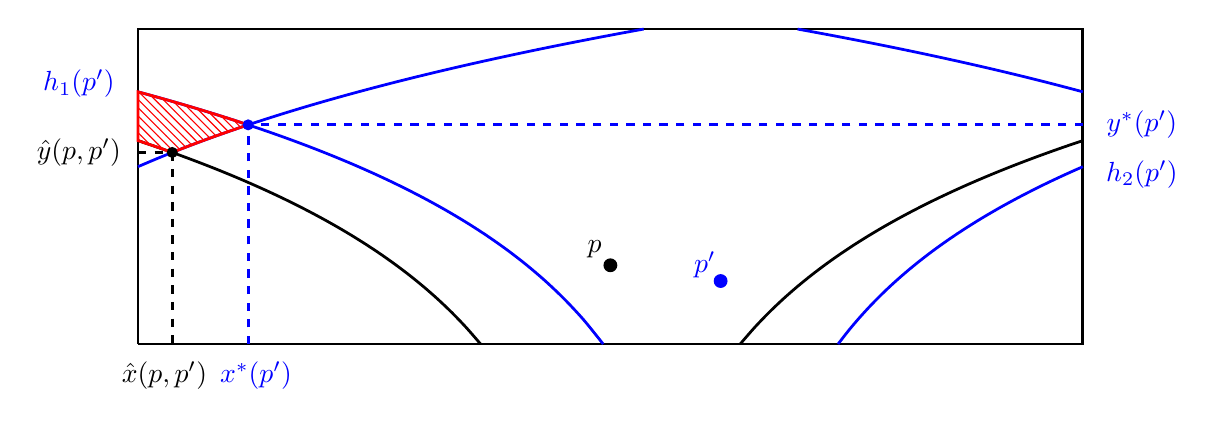
\begin{tikzpicture}
	%Define the coordinates 
	%p = (\u,\v) and p^\prime = (\uu, \vv)
	%Box \Rcal has width 2\r and height \t
	\pgfmathsetmacro{\u}{0} %0
	\pgfmathsetmacro{\v}{1} %1
	\pgfmathsetmacro{\uu}{1.4} %1.4
	\pgfmathsetmacro{\vv}{0.8} %0.8
	\pgfmathsetmacro{\r}{6}
	\pgfmathsetmacro{\t}{4}
	
	%The box \Rcal
	\draw[line width=1pt] (-\r,0) -- (\r,0) -- (\r,\t) -- (-\r,\t) -- (-\r,0);

	%Dram both nodes
    \draw node[fill, circle, inner sep=0pt, minimum size=5pt] (p1) at (\u,\v) {};
    \path (p1)+(-0.2,0.2) node {$p$};
    \draw node[fill,blue, circle, inner sep=0pt, minimum size=5pt] (p2) at (\uu,\vv) {};
    \path (p2)+(-0.2,0.2) node {\color{blue}$p^\prime$};
	
	
	%Boundaries p = (\u,\v)
	
	%Right boundary
	\pgfmathsetmacro{\rightbounduv}{\u+exp((\v)/2)}
	\draw[domain=\rightbounduv:\r,smooth,variable=\x,black,line width=1pt] plot (\x, {2*ln(\x)-\v});
    %Left boundary
    \pgfmathsetmacro{\leftbounduv}{\u-exp((\v)/2)}
    \draw[domain=\leftbounduv:-\r,smooth,variable=\x,black,line width=1pt] plot (\x, {2*ln(-\x)-\v});
    
    %Boundaries p^\prime = (\uu,\vv)
    
    %Right boundary
    \pgfmathsetmacro{\rightbounduuvv}{\uu+exp((\vv)/2)}
    \draw[domain=\rightbounduuvv:\r,smooth,variable=\x,blue,line width=1pt] plot (\x, {2*ln(\x-\uu)-\vv});
    %Shifted right boundary
    \pgfmathsetmacro{\shiftrightbounduuvv}{\uu+exp((\vv + \t)/2)-2*\r}
    \draw[domain=\shiftrightbounduuvv:-\r,smooth,variable=\x,blue,line width=1pt] plot (\x, {2*ln(\x+(2*\r-\uu))-\vv});
    %Left boundary 
    \pgfmathsetmacro{\leftbounduuvv}{\uu-exp((\vv)/2)}
    \draw[domain=\leftbounduuvv:-\r,smooth,variable=\x,blue,line width=1pt] plot (\x, {2*ln(\uu-\x)-\vv});
    %Shifted left boundary
    \pgfmathsetmacro{\shiftleftbounduuvv}{\uu-exp((\vv + \t)/2)+2*\r}
    \draw[domain=\shiftleftbounduuvv:\r,smooth,variable=\x,blue,line width=1pt] plot (\x, {2*ln(2*\r + \uu-\x)-\vv});
    
    %Define x^\ast(p^\prime) and y^\ast(p^\prime)
    \pgfmathsetmacro{\uuast}{\uu-\r}
    \pgfmathsetmacro{\vvast}{2*ln(\r)-\vv}
    
    %Define intersection left black and shifted blue curve
    \pgfmathsetmacro{\vast}{2*ln((2*\r - \uu)/(exp(\v/2) + exp(\vv/2)))}
    \pgfmathsetmacro{\uast}{(\uu - 2*\r)/(1 + exp((\vv - \v)/2))}    
   
    %Define h_1(p) = h_2(p)
    \pgfmathsetmacro{\hp}{2*ln(\r-\u)-\v}
    
    %Define h_1(p^\prime) and h_2(p^\prime)
    \pgfmathsetmacro{\hh}{2*ln(\uu+\r)-\vv}
    \pgfmathsetmacro{\hhh}{2*ln(\r-\uu)-\vv}
    
    %Highlight area between left black, left blue and shifted right blue line
	\draw[red,line width=1pt,pattern=north west lines, pattern color=red] 
		plot[domain=\uuast:\uast,smooth,variable=\x,red] (\x, {2*ln(\x+(2*\r-\uu))-\vv}) 
		-- 
		plot[domain=\uast:-\r,smooth,variable=\x,red] (\x, {2*ln(-\x)-\v})
		-- 
		(-\r,\hh)
		-- 
		plot[domain=-\r:\uuast,smooth,variable=\x,red] (\x, {2*ln(\uu-\x)-\vv});
	
%	\draw node[fill, circle, inner sep=0pt, minimum size=4pt, blue] at (\uuast,\vvast) {};
%	\draw node[fill, circle, inner sep=0pt, minimum size=4pt, black] at (\uast,\vast) {};
%	\draw node (f1) at (\uuast,\vvast+0.9) {\color{blue}$(x^\ast(p^\prime), y^\ast(p^\prime))$};
%	\draw node (f2) at (\uast+1,\vast-1.25) {\color{black}$(\hat{x}(p,p^\prime), \hat{y}(p,p^\prime))$};
%	
%	\draw[->,thick] (f2) -- (\uast+0.1,\vast-0.2);
%	\draw[->,thick,blue] (f1) -- (\uuast,\vvast+0.2);
	
	 \draw[dashed,line width=1pt,blue] (\uuast,0) -- (\uuast,\vvast);
	 \draw node at (\uuast+0.1,-0.4) {\color{blue}$x^\ast(p^\prime)$};
	 \draw[dashed,line width=1pt,blue] (\r,\vvast) -- (\uuast,\vvast);
	 \draw node at (\r+0.75,\vvast) {\color{blue}$y^\ast(p^\prime)$};
	 \draw[dashed,black,line width=1pt] (-\r,\vast) -- (\uast,\vast);
	 \draw node at (-\r-0.75,\vast) {\color{black}$\hat{y}(p,p^\prime)$};
	 \draw[dashed,black,line width=1pt] (\uast,\vast) -- (\uast,0);
	 \draw node at (\uast-0.1,-0.4) {\color{black}$\hat{x}(p,p^\prime)$};
	 
	 \draw node[fill, circle, inner sep=0pt, minimum size=4pt, blue] at (\uuast,\vvast) {};
	 \draw node[fill, circle, inner sep=0pt, minimum size=4pt, black] at (\uast,\vast) {};
	
    \draw node at (-\r-0.75,\hh+0.1) {\color{blue}$h_1(p^\prime)$};
    \draw node at (\r+0.75,\hhh-0.1) {\color{blue}$h_2(p^\prime)$};

\end{tikzpicture}
\caption{Example configuration of two points $p$ and $p^\prime$ for which $\BallPon{p} \cap \BallPon{p^\prime}$ is not a subset of $\BallPo{p} \cap \BallPo{p^\prime}$. The red region indicates the area belonging to $\BallPon{p} \cap \BallPon{p^\prime}$ but not to $\BallPo{p} \cap \BallPo{p^\prime}$.}
\label{fig:comparing_triangles_diff_intersections}
\end{figure}

Recall that $\mathcal{T}_{\Pcal \Delta \Pcal_n}(p,p^\prime)$ denotes the region of points which form triangles with $p$ and $p^\prime$ in $\Gbox$ but not in $\Ginf$. Figure \ref{fig:comparing_triangles_diff_intersections} shows an example of a configuration where $\mathcal{T}_{\Pcal \Delta \Pcal_n}(p,p^\prime) \ne \emptyset$. We observe that $\mathcal{T}_{\Pcal \Delta \Pcal_n}(p,p^\prime) \ne \emptyset$ because the right boundary of the ball $\BallPon{p^\prime}$ exists the right boundary of the box $\Rcal$ and then, since we identified the boundaries, continues from the left so that $\BallPon{p^\prime}$ covers part of the ball $\BallPon{p}$ which would not be covered in the infinite limit model. 

To further analyze this, let us introduce some notation. For any $p = (x,y) \in \Rcal$ we will define the left and right boundary functions as, respectively,
\begin{align}
	b_p^-(z) &= \begin{cases}
		2 \log\left(x-z\right) - y &\mbox{if }  -\frac{\pi}{2} e^{R_n/2} \le z \le x - e^{y/2}  \\
		2\log\left(\pi e^{R_n/2} + x - z\right) - y 
			&\mbox{if } x - e^{(y + R_n)/2} + \pi e^{R_n/2} \le z \le \frac{\pi}{2} e^{R_n/2}\\
		0 &\mbox{else}
	\end{cases}\\
	b_p^+(z) &= \begin{cases}
		2 \log\left(z-x\right) - y &\mbox{if } x + e^{y/2} \le z \le \frac{\pi}{2} e^{R_n/2} \\
		2\log\left(\pi e^{R_n/2} + z - x\right) - y 
			&\mbox{if } -\frac{\pi}{2} e^{R_n/2} \le z \le x + e^{(y + R_n)/2} - \pi e^{R_n/2}\\
		0 &\mbox{else}
	\end{cases}
\end{align}
Note that these functions describe the boundaries of the ball $\BallPon{p}$. In particular, $p^\prime = (x^\prime, y^\prime) \in \BallPon{p}$ if and only if $y^\prime \ge \min\left\{b_p^-(x^\prime), b_p^+(x^\prime)\right\}$.

Since we have identified the left and right boundary of $\Rcal$ we can assume, without loss of generality that $x = 0$. Due to symmetry it is then enough to restrict the analysis to the case where $x^\prime > 0$. \TM{ does this not depend on $p$? }\PvdH{I do not think so, because we can always take $p = (0,y)$ due to the invariance in the $x$-direction. I have updated the text to better reflect this.} 
For this case there are two important points in the box $\Rcal$. These are the intersection between the left boundary of $p^\prime$ and the right boundary of $p^\prime$, as it continues from the left side of the box, and the left boundary of $p$. We denote by $(x^\ast(p^\prime), y^\ast(p^\prime))$ the intersection between the left and right boundary of $p^\prime$ and by $(\hat{x}(p,p^\prime), \hat{y}(p,p^\prime))$ the intersection between the left boundary of $p$ and the right boundary of $p^\prime$, see Figure \ref{fig:comparing_triangles_diff_intersections}. 

Let us derive the expressions for the coordinates of these two points, starting with $(x^\ast(p^\prime), y^\ast(p^\prime))$. The $x$-coordinate $x^\ast(p^\prime)$ is the solution to the equation $b_{p^\prime}^+(z) = b_{p^\prime}^-(z)$ for $-\frac{\pi}{2} e^{R_n/2} \le z \le x + e^{(y + R_n)/2} - \pi e^{R_n/2}$. This equation becomes
\[
	2\log\left(\pi e^{R_n/2} + z - x^\prime\right) - y^\prime = 2 \log\left(x^\prime-z\right) - y^\prime,
\]
whose solution is $x^\ast(p^\prime) := x^\prime - \frac{\pi}{2} e^{R_n/2}$. Plugging this into either the left or right hand side of the above equation yields the $y$-coordinate $y^\ast(p^\prime) = 2\log\left(\frac{\pi}{2}e^{R_n/2}\right) - y^\prime$. In a similar way, the $x$-coordinate $\hat{x}(p,p^\prime)$ is the solution to the equation $b_{p^\prime}^+(z) = b_{p}^-(z)$ for $-\frac{\pi}{2} e^{R_n/2} \le z \le x + e^{(y + R_n)/2} - \pi e^{R_n/2}$, i.e.
\[
	2\log\left(\pi e^{R_n/2} + z - x^\prime\right) - y^\prime = 2 \log\left(x-z\right) - y.
\] 
This solution is $\frac{x^\prime - \pi e^{R_n/2}}{1 + e^{(y^\prime - y)/2}}$ and again $\hat{y}(p,p^\prime)$ is obtained by plugging the solution into either the left or right hand side of the equation, yielding $\hat{y}(p,p^\prime) = 2 \log\left(\frac{\pi e^{R_n/2} - x^\prime}{e^{y/2} + e^{y^\prime/2}}\right)$.

To summarize we have:
% After some simple algebra \TM{ I am not a big fan of writing "after some simple algebra" or similar. This is how errors can creep into your argument. Maybe we can just give the details? } we obtain the following expressions for the coordinates of these two points
\begin{align*}
	x^\ast(p^\prime) &= x^\prime - \frac{\pi}{2} e^{R_n/2}\\
	y^\ast(p^\prime) &= 2\log\left(\frac{\pi}{2}e^{R_n/2}\right) - y^\prime\\
	\hat{x}(p,p^\prime) &= \frac{x^\prime - \pi e^{R_n/2}}{1 + e^{(y^\prime - y)/2}} \\
	\hat{y}(p,p^\prime) &= 2 \log\left(\frac{\pi e^{R_n/2} - x^\prime}{e^{y/2} + e^{y^\prime/2}}\right)
\end{align*}

The crucial observation is that $\mathcal{T}_{\Pcal \Delta \Pcal_n} = \emptyset$ as long as the point $(x^\ast(p^\prime), y^\ast(p^\prime))$ is above the left boundary of $p$. This happens exactly when $y^\ast(p^\prime) > b_p^-(x^\ast(p^\prime))$. Therefore the boundary of this event is given by the equation $y^\ast(p^\prime) = b_p^-(x^\ast(p^\prime))$ which reads
\[
	2\log\left(\frac{\pi}{2}e^{R_n/2}\right) - y^\prime = 2\log\left(\frac{\pi}{2} e^{R_n/2} -x^\prime\right) - y.
\]
Solving this equation gives us the function
\begin{equation}
	b^\ast_p(z) = y - 2\log\left(1 - \frac{z}{\frac{\pi}{2} e^{R_n/2}}\right),
\end{equation}
which is displayed by the red curve in Figure \ref{fig:comparing_triangles_diff_analysis}. It holds that $y^\ast(p^\prime) > b_p^-(x^\ast(p^\prime))$ if and only if $y^\prime < b^\ast_p(x^\prime)$ and hence we have that $\mathcal{T}_{\Pcal \Delta \Pcal_n} = \emptyset$ for all $p^\prime \in \Rcal$ for which $y^\prime \ge b^\ast_p(x^\prime)$. We also note that when $y^\prime = b^\ast_p(x^\prime)$ the two points $(x^\ast(p^\prime), y^\ast(p^\prime))$ and $(\hat{x}(p,p^\prime),\hat{y}(p,p^\prime))$ coincide.



\begin{figure}[!t]

\centering
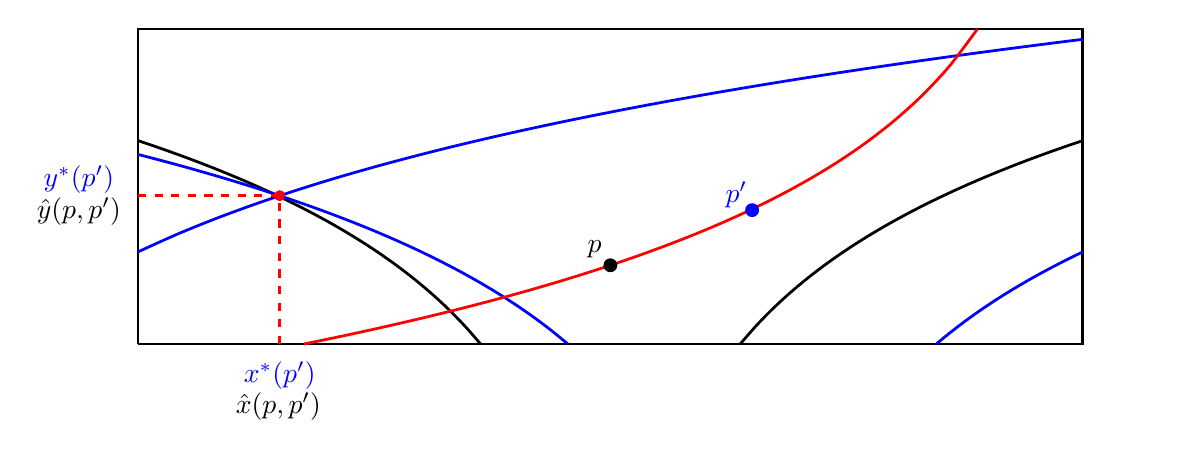
\begin{tikzpicture}
	%Define the coordinates 
	%p = (\u,\v) and p^\prime = (\uu, \vv)
	%Box \Rcal has width 2\r and height \t
	\pgfmathsetmacro{\u}{0}
	\pgfmathsetmacro{\v}{1}
	\pgfmathsetmacro{\uu}{1.8}
	\pgfmathsetmacro{\vv}{1.7}
	\pgfmathsetmacro{\r}{6}
	\pgfmathsetmacro{\t}{4}
	
	%The box \Rcal
	\draw[line width=1pt] (-\r,0) -- (\r,0) -- (\r,\t) -- (-\r,\t) -- (-\r,0);	
	
	%Boundaries p = (\u,\v)
	
	%Right boundary
	\pgfmathsetmacro{\rightbounduv}{\u+exp((\v)/2)}
	\draw[domain=\rightbounduv:\r,smooth,variable=\x,black,line width=1pt] plot (\x, {2*ln(\x)-\v});
    %Left boundary
    \pgfmathsetmacro{\leftbounduv}{\u-exp((\v)/2)}
    \draw[domain=\leftbounduv:-\r,smooth,variable=\x,black,line width=1pt] plot (\x, {2*ln(-\x)-\v});
    
    %Boundaries p^\prime = (\uu,\vv)
    
    %Right boundary
    \pgfmathsetmacro{\rightbounduuvv}{\uu+exp((\vv)/2)}
    \draw[domain=\rightbounduuvv:\r,smooth,variable=\x,blue,line width=1pt] plot (\x, {2*ln(\x-\uu)-\vv});
    %Shifted right boundary
    \pgfmathsetmacro{\shiftrightbounduuvv}{\uu+exp((\vv + \t)/2)-2*\r}
    %\draw[domain=\shiftrightbounduuvv:-\r,smooth,variable=\x,blue,line width=1pt] plot (\x, {2*ln(\x+(2*\r-\uu))-\vv});
    \draw[domain=-\r:\r,smooth,variable=\x,blue,line width=1pt] plot (\x, {2*ln(\x+(2*\r-\uu))-\vv});
    %Left boundary 
    \pgfmathsetmacro{\leftbounduuvv}{\uu-exp((\vv)/2)}
    \draw[domain=\leftbounduuvv:-\r,smooth,variable=\x,blue,line width=1pt] plot (\x, {2*ln(\uu-\x)-\vv});
    %Shifted left boundary

    
    %Star boundary
    \pgfmathsetmacro{\starleftbound}{\r*(1-exp(\v/2))}
    \pgfmathsetmacro{\starrightbound}{\r*(1-exp((\v-\t)/2))}
    \draw[domain=\starleftbound:\starrightbound,smooth,variable=\x,red, line width=1pt] plot (\x, {2*ln((\r/(\r-\x)))+\v});
    
    %Define h_1(p) = h_2(p)
    \pgfmathsetmacro{\hp}{2*ln(\r-\u)-\v}
%    \draw node at (\r+0.75,\hp) {\color{black}$h(y)$};
    \draw node at (\r+1,\hp) {};
    
    %Define h_1(p^\prime) and h_2(p^\prime)
    \pgfmathsetmacro{\hh}{2*ln(\uu+\r)-\vv}
    \pgfmathsetmacro{\hhh}{2*ln(\r-\uu)-\vv}

%    \draw node at (-\r-0.75,\hh+0.1) {\color{blue}$h_1(p^\prime)$};
%    \draw node at (\r+0.75,\hhh) {\color{blue}$h_2(p^\prime)$};
    
    %Define x^\ast(p^\prime) and y^\ast(p^\prime), intersection of left and shifted right blue curve
    \pgfmathsetmacro{\uuast}{\uu-\r}
    \pgfmathsetmacro{\vvast}{2*ln(\r)-\vv}

    %Define intersection left black and shifted blue curve
    \pgfmathsetmacro{\vast}{2*ln((2*\r - \uu)/(exp(\v/2) + exp(\vv/2)))}
    \pgfmathsetmacro{\uast}{(\uu - 2*\r)/(1 + exp((\vv - \v)/2))} 

%    \draw[dashed,thick,black] (-\r,\hhh) -- (\r,\hhh);
    \draw[dashed,line width=1pt,red] (\uuast,0) -- (\uuast,\vvast);
    \draw node at (\uuast,-0.4) {\color{blue}$x^\ast(p^\prime)$};
    \draw[dashed,line width=1pt,red] (-\r,\vvast) -- (\uuast,\vvast);
    \draw node at (-\r-0.75,\vvast+0.2) {\color{blue}$y^\ast(p^\prime)$};
%    \draw[dashed,black,line width=1pt] (-\r,\vast) -- (\uast,\vast);
    \draw node at (-\r-0.75,\vast-0.2) {\color{black}$\hat{y}(p,p^\prime)$};
%    \draw[dashed,black,line width=1pt] (\uast,\vast) -- (\uast,0);
    \draw node at (\uast,-0.8) {\color{black}$\hat{x}(p,p^\prime)$};
    
    \draw node[fill, circle, inner sep=0pt, minimum size=4pt, red] at (\uuast,\vvast) {};
    
   	%Draw both nodes
    \draw node[fill, circle, inner sep=0pt, minimum size=5pt] (p1) at (\u,\v) {};
    \path (p1)+(-0.2,0.2) node {$p$};
    \draw node[fill,blue, circle, inner sep=0pt, minimum size=5pt] (p2) at (\uu,\vv) {};
    \path (p2)+(-0.2,0.2) node {\color{blue}$p^\prime$};
    
    
    
%    \draw node[fill, circle, inner sep=0pt, minimum size=4pt, black] at (\uast,\vast) {};
    
%    \draw node at (-7,2.5835) {$h(y)$};

    
%    \draw[dotted,thick,black] (4.5208,2.0174) -- (4.5208,0);
%    \draw[dotted,thick,black] (4.5208,2.0174) -- (6,2.0174);
    
%    \draw node at (4.5208,-0.5) {$w_x(p,p^\prime)$};
%    \draw node at (7,2.0174) {$w_y(p,p^\prime)$};
    
%    \draw node at (0,3.5) {\color{blue}$x_1 = x^\prime + e^{\frac{y^\prime + y_1}{2}}$};
%    \draw node at (-2,1.6) {\color{blue}$x_1 = x^\prime - e^{\frac{y^\prime + y_1}{2}}$};
%    \draw node at (-4.5,1) {$x_1 = x - e^{\frac{y + y_1}{2}}$};
%    \draw node at (2,1.5) {$x_1 = x + e^{\frac{y + y_1}{2}}$};

\end{tikzpicture}
\caption{Example for a given $p$ of the boundary function $x^\prime \mapsto b^\ast_p(x^\prime)$, given by the red curve, which determines whether $\mathcal{T}_{\Pcal \Delta \Pcal_n} = \emptyset$. We see that when $y^\prime = b^\ast_p(x^\prime)$ then $(\hat{x}(p,p^\prime), \hat{y}(p,p^\prime)) = (x^\ast(p^\prime), y^\ast(\prime))$.}
\label{fig:comparing_triangles_diff_analysis}
\end{figure}

This analysis allows us to compute the expected difference in the number of triangles for the finite box model and the infinite model, for a typical node with height $y$, i.e. prove Lemma~\ref{lem:clustering_error_T_term}. 

\begin{figure}[!t]

\centering
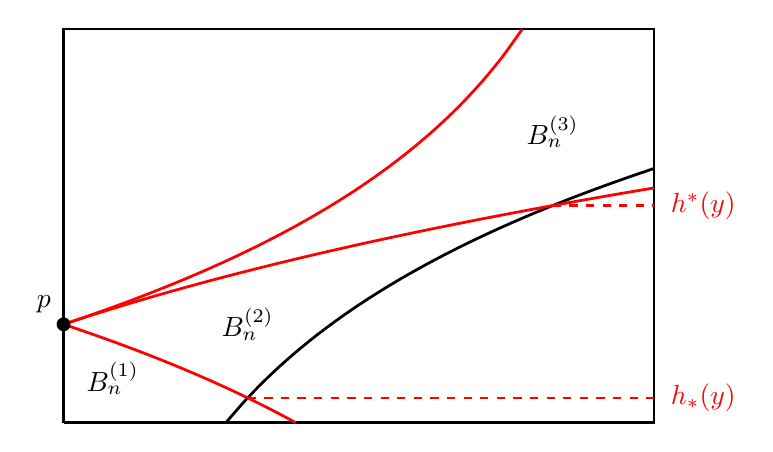
\begin{tikzpicture}[scale=1.25]

%%%%%%%%%%%%%%%%%%%%%%%%%%%%%%%%%%%%%%%%%%%%%%%%%%%%%%%%%%%%%%%%%%%%%%%%%%%%%%%%%%%%%%%%%%%%%%%%%%%
%																								  %
%	Shows the three different areas B_n^{(i)} for the computations in Lemma 					  %
%	\label{lem:clustering_error_T_term}			  												  %
%																								  %
%%%%%%%%%%%%%%%%%%%%%%%%%%%%%%%%%%%%%%%%%%%%%%%%%%%%%%%%%%%%%%%%%%%%%%%%%%%%%%%%%%%%%%%%%%%%%%%%%%%

	%Define the coordinates 
	%p = (\u,\v) and p^\prime = (\uu, \vv)
	%Box \Rcal has width 2\r and height \t
	\pgfmathsetmacro{\u}{0}
	\pgfmathsetmacro{\v}{1}
	\pgfmathsetmacro{\uu}{1.8}
	\pgfmathsetmacro{\vv}{1.7}
	\pgfmathsetmacro{\r}{6}
	\pgfmathsetmacro{\t}{4}
	
	%The box \Rcal only positive x
	\draw[line width=1pt] (0,0) -- (\r,0) -- (\r,\t) -- (0,\t) -- (0,0);	
	
	%Boundaries p = (\u,\v)
	
	%Right boundary
	\pgfmathsetmacro{\rightbounduv}{\u+exp((\v)/2)}
	\draw[domain=\rightbounduv:\r,smooth,variable=\x,black,line width=1pt] plot (\x, {2*ln(\x)-\v});
    %Left boundary
%    \pgfmathsetmacro{\leftbounduv}{\u-exp((\v)/2)}
%    \draw[domain=\leftbounduv:-\r,smooth,variable=\x,black,line width=1pt] plot (\x, {2*ln(-\x)-\v});
    
    %Three boundaries for the regions B_n
    \pgfmathsetmacro{\bone}{\r*(1-exp(-\v/2))}
    \pgfmathsetmacro{\btwo}{\r*(exp(-\v/2)-1)}
    %Star boundary
    \pgfmathsetmacro{\bthreeleft}{\r*(1-exp(\v/2))}
    \pgfmathsetmacro{\bthreeright}{\r*(1-exp((\v-\t)/2))}
    
    \draw[domain=0:\bone,smooth,variable=\x,red,line width=1pt] plot (\x, {\v-2*ln(\r/(\r-\x))});
    \draw[domain=0:\r,smooth,variable=\x,red,line width=1pt] plot (\x, {\v+2*ln(1+(\x/\r))});
    \draw[domain=0:\bthreeright,smooth,variable=\x,red, line width=1pt] plot (\x, {2*ln((\r/(\r-\x)))+\v});    
    
    %Define the top and bottom coordinates of y^prime boundaries
    \pgfmathsetmacro{\ybottom}{\v+2*ln(\r/(\r+exp(\v)))}
    \pgfmathsetmacro{\xbottom}{\r*exp(\v)/(\r + exp(\v))}
    \pgfmathsetmacro{\ytop}{\v+2*ln(\r/(\r-exp(\v)))}
    \pgfmathsetmacro{\xtop}{\r*exp(\v)/(\r - exp(\v))}
    
    \draw[dashed,line width=1pt,red] (\xbottom,\ybottom) -- (\r,\ybottom);
    \draw[dashed,line width=1pt,red] (\xtop,\ytop) -- (\r,\ytop);
    \draw node at (\r+0.5,\ybottom) {\color{red}$h_\ast(y)$};
    \draw node at (\r+0.5,\ytop) {\color{red}$h^\ast(y)$};
    
    \draw node at (0.5,\ybottom+0.2) {$B_n^{(1)}$};
    \draw node at (\xbottom,\ybottom+0.75) {$B_n^{(2)}$};
    \draw node at (\xtop,\ytop+0.75) {$B_n^{(3)}$};
    

    %Define h_1(p) = h_2(p)
    \pgfmathsetmacro{\hp}{2*ln(\r-\u)-\v}
  
    %Define h_1(p^\prime) and h_2(p^\prime)
    \pgfmathsetmacro{\hh}{2*ln(\uu+\r)-\vv}
    \pgfmathsetmacro{\hhh}{2*ln(\r-\uu)-\vv}

%    \draw node at (-\r-0.75,\hh+0.1) {\color{blue}$h_1(p^\prime)$};
%    \draw node at (\r+0.75,\hhh) {\color{blue}$h_2(p^\prime)$}; 
    
   	%Draw node p
    \draw node[fill, circle, inner sep=0pt, minimum size=5pt] (p1) at (\u,\v) {};
    \path (p1)+(-0.2,0.2) node {$p$};

\end{tikzpicture}
\caption{Three different areas $B_n^{(i)}$ used in the proof of Lemma \ref{lem:clustering_error_T_term}.}
\label{fig:comparing_triangles_B_areas}
\end{figure}

\begin{proof}[Proof of Lemma \ref{lem:clustering_error_T_term}]
Due to symmetry it is enough to show that
\begin{equation}\label{eq:clustering_error_T_main}
	\int_0^{R_n}\int_0^{I_n} \mu\left(\mathcal{T}_{\Pcal \Delta \Pcal_n}(p,p_1)\right) f(x_1,y_1) 
	\dd x_1 \dd y_1 = \bigO{y n^{-(2\alpha - 1)} + n^{-(2\alpha-1)} e^{y}}
\end{equation}
The proof goes in two stages. First we compute $\mu\left(\mathcal{T}_{\Pcal \Delta \Pcal_n}(p,p_1)\right)$ by splitting it over three disjoint regimes with respect to $p_1$, with $x_1 \ge 0$. Then we do the integration with respect to $p_1$.

\subsubsection*{Computing $\bm{\mu\left(\mathcal{T}_{\Pcal \Delta \Pcal_n}(p,p_1)\right)}$}

Recall that $I_n = \frac{\pi}{2} e^{R_n/2}$ and define the sets
\begin{align*}
	A_n^{(1)} &= \left\{p_1 \in \Rcal \, : \, 0 \le y_1 \le y - 2\log(I_n/(I_n-x_1)) \right\},\\
	A_n^{(2)} &= \left\{p_1 \in \Rcal \, : \, y - 2\log(I_n/(I_n-x_1)) < y_1 
		\le y + 2 \log\left(1 + \frac{x_1}{I_n}\right)\right\},\\
	A_n^{(3)} &= \left\{p_1 \in \Rcal \, : \, y + 2 \log\left(1 + \frac{x_1}{I_n}\right) < y_1 
			\le y + 2 \log\left(\frac{I_n}{I_n-x_1}\right)\right\},
\end{align*}
and let $B_n^{(i)} = \BallPon{p} \cap A_n^{(i)}$, for $i = 1, 2, 3$, see Figure~\ref{fig:comparing_triangles_B_areas}. Here the heights of the two intersections are given by
\begin{align}
	h_\ast(y) &= y + 2 \log\left(\frac{I_n}{I_n + e^y}\right)\\
	h^\ast(y) &= y + 2 \log\left(\frac{I_n}{I_n - e^y}\right).
\end{align}

With these definitions we have that the union $B_n := \bigcup_{i = 1}^n B_n^{(i)}$ denotes the area under the red curve in Figure~\ref{fig:comparing_triangles_diff_analysis} and hence, for all $p_1 \in \Rcal\setminus B_n$ with $x_1 \ge 0$ we have that $\mathcal{T}_{\Pcal \Delta \Pcal_n}(p,p_1) = \emptyset$. So we only need to consider $p_1 \in B_n$. We shall establish the following result:
\begin{equation}\label{eq:mu_triangle_diff}
	\mu\left(\mathcal{T}_{\Pcal \Delta \Pcal_n}(p,p_1)\right) = 
	\begin{cases}
		\bigO{I_n^{-2\alpha} e^{\alpha y_1}} &\mbox{if } p_1 \in B_n^{(1)}\\
		\bigO{I_n^{-2\alpha} e^{\alpha y}} &\mbox{if } p_1 \in B_n^{(2)} \cup B_n^{(3)}
	\end{cases}
\end{equation}

Depending on which regime $p_1$ belongs to, the set $\mathcal{T}_{\Pcal \Delta \Pcal_n}(p,p_1)$ has a different shape. We displayed these shapes in Figure~\ref{fig:shapes_triangle_mismatches} as a visual aid to follow the computations below. 

\begin{figure}[!tp]
\centering
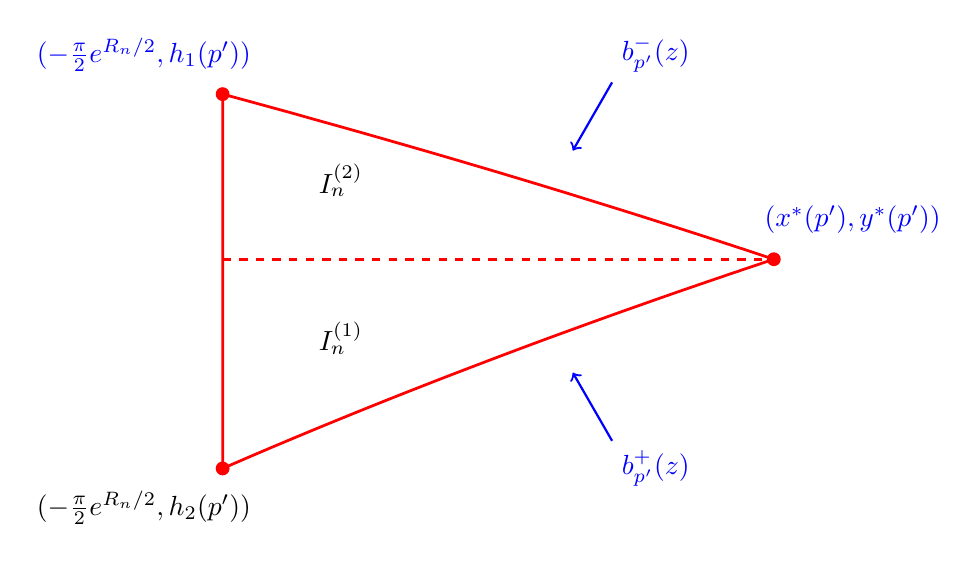
\begin{tikzpicture}[scale=5]

%%%%%%%%%%%%%%%%%%%%%%%%%%%%%%%%%%%%%%%%%%%%%%%%%%%%%%%%%%%%%%%%%%%%%%%%%%%%%%%%%%%%%%%%%%%%%%%%%%%
%																								  %
%	Shows the area T_{\Pcal \Delta \Pcal_n} when h_1(p^\prime) > h_2(p^\prime) > h(y)			  %
%																								  %
%%%%%%%%%%%%%%%%%%%%%%%%%%%%%%%%%%%%%%%%%%%%%%%%%%%%%%%%%%%%%%%%%%%%%%%%%%%%%%%%%%%%%%%%%%%%%%%%%%%

	%Define the coordinates 
	%p = (\u,\v) and p^\prime = (\uu, \vv)
	%Box \Rcal has width 2\r and height \t
	\pgfmathsetmacro{\u}{0}
	\pgfmathsetmacro{\v}{1}
	\pgfmathsetmacro{\uu}{1.4}
	\pgfmathsetmacro{\vv}{0.2}
	\pgfmathsetmacro{\r}{6}
	\pgfmathsetmacro{\t}{4}
    
    %Define x^\ast(p^\prime) and y^\ast(p^\prime)
    \pgfmathsetmacro{\uuast}{\uu-\r}
    \pgfmathsetmacro{\vvast}{2*ln(\r)-\vv}
    
    %Define intersection left black and shifted blue curve
    \pgfmathsetmacro{\vast}{2*ln((2*\r - \uu)/(exp(\v/2) + exp(\vv/2)))}
    \pgfmathsetmacro{\uast}{(\uu - 2*\r)/(1 + exp((\vv - \v)/2))}    
   
    %Define h_1(p) = h_2(p)
    \pgfmathsetmacro{\hp}{2*ln(\r-\u)-\v}
    
    %Define h_1(p^\prime) and h_2(p^\prime)
    \pgfmathsetmacro{\hh}{2*ln(\uu+\r)-\vv}
    \pgfmathsetmacro{\hhh}{2*ln(\r-\uu)-\vv}
    
    %Draw the boundary left black, left blue and shifted right blue line
	\draw[red,line width=1pt] 
		plot[domain=\uuast:-\r,smooth,variable=\x,red] (\x, {2*ln(\x+(2*\r-\uu))-\vv}) 
		-- 
		(-\r,\hh)
		-- 
		plot[domain=-\r:\uuast,smooth,variable=\x,red] (\x, {2*ln(\uu-\x)-\vv});
	
	\pgfmathsetmacro{\top}{2*ln(\uu-\uast)-\vv}
	
	\draw[red, dashed,line width=1pt] (-\r,\vvast) -- (\uuast,\vvast);

    \draw node at (-\r-0.2,\hh+0.1) {\color{blue}$(-\frac{\pi}{2} e^{R_n/2}, h_1(p^\prime))$};
    \draw node at (-\r-0.2,\hhh-0.1) {$(-\frac{\pi}{2} e^{R_n/2}, h_2(p^\prime))$};
    \draw node at (\uuast+0.2,\vvast+0.1) {\color{blue}$(x^\ast(p^\prime), y^\ast(p^\prime))$};
    
    \draw node at (-\r+0.3,\vvast+0.2) {$I_n^{(2)}$};
    \draw node at (-\r+0.3,\vvast-0.2) {$I_n^{(1)}$};
    
    \draw node (f2) at (\uuast-0.3,\hh+0.1) {\color{blue}$b_{p^\prime}^-(z)$};
    \draw node (f3) at (\uuast-0.3,\hhh) {\color{blue}$b_{p^\prime}^+(z)$};
    \path (f2)+(230:0.35) node (f2_arrow) {};
    \path (f3)+(130:0.35) node (f3_arrow) {};
    \draw[->,thick,blue] (f2.south west) -- (f2_arrow);
    \draw[->,thick,blue] (f3.north west) -- (f3_arrow);

	\draw node[red, fill, circle, inner sep=0pt, minimum size=5pt] at (-\r,\hhh) {};
	\draw node[red, fill, circle, inner sep=0pt, minimum size=5pt] at (-\r,\hh) {};
	\draw node[red, fill, circle, inner sep=0pt, minimum size=5pt] at (\uuast,\vvast) {};

\end{tikzpicture}\\
\vspace{20pt}
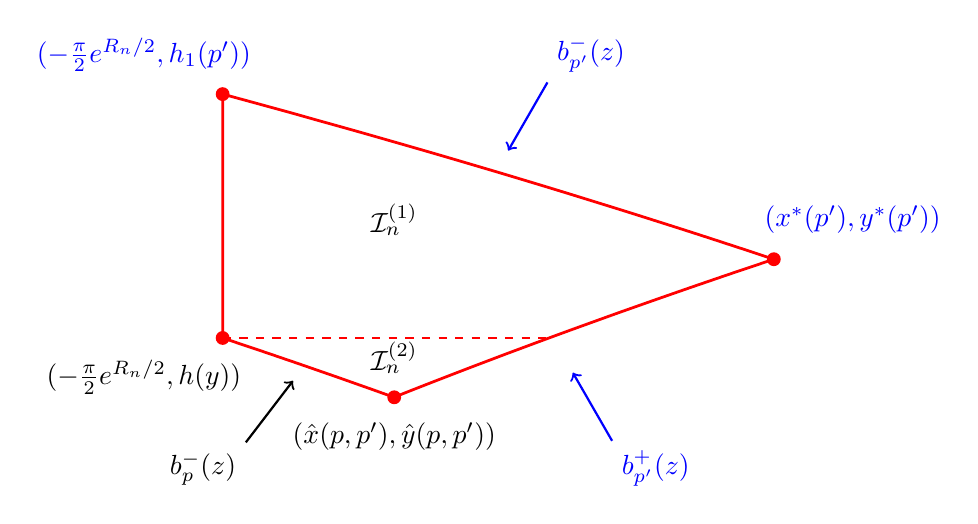
\begin{tikzpicture}[scale=5]
	%Define the coordinates 
	%p = (\u,\v) and p^\prime = (\uu, \vv)
	%Box \Rcal has width 2\r and height \t
	\pgfmathsetmacro{\u}{0}
	\pgfmathsetmacro{\v}{1}
	\pgfmathsetmacro{\uu}{1.4}
	\pgfmathsetmacro{\vv}{0.8}
	\pgfmathsetmacro{\r}{6}
	\pgfmathsetmacro{\t}{4}
    
    %Define x^\ast(p^\prime) and y^\ast(p^\prime)
    \pgfmathsetmacro{\uuast}{\uu-\r}
    \pgfmathsetmacro{\vvast}{2*ln(\r)-\vv}
    
    %Define intersection left black and shifted blue curve
    \pgfmathsetmacro{\vast}{2*ln((2*\r - \uu)/(exp(\v/2) + exp(\vv/2)))}
    \pgfmathsetmacro{\uast}{(\uu - 2*\r)/(1 + exp((\vv - \v)/2))}    
   
    %Define h_1(p) = h_2(p)
    \pgfmathsetmacro{\hp}{2*ln(\r-\u)-\v}
    
    %Define h_1(p^\prime) and h_2(p^\prime)
    \pgfmathsetmacro{\hh}{2*ln(\uu+\r)-\vv}
    \pgfmathsetmacro{\hhh}{2*ln(\r-\uu)-\vv}
    
    %Draw the boundary left black, left blue and shifted right blue line
	\draw[red,line width=1pt] 
		plot[domain=\uuast:\uast,smooth,variable=\x,red] (\x, {2*ln(\x+(2*\r-\uu))-\vv}) 
		-- 
		plot[domain=\uast:-\r,smooth,variable=\x,red] (\x, {2*ln(-\x)-\v})
		-- 
		(-\r,\hh)
		-- 
		plot[domain=-\r:\uuast,smooth,variable=\x,red] (\x, {2*ln(\uu-\x)-\vv});
	
	\pgfmathsetmacro{\rb}{\uu + exp((\vv+\hp)/2) -2*\r}
	

	%\draw[red,dashed,line width=1pt] (\uast,\vast) -- (\uast,\hp);
	\draw[red,dashed,line width=1pt] (-\r,\hp) -- (\rb,\hp);

    \draw node at (-\r-0.2,\hh+0.1) {\color{blue}$(-\frac{\pi}{2} e^{R_n/2}, h_1(p^\prime))$};
    \draw node at (-\r-0.2,\hp-0.1) {$(-\frac{\pi}{2} e^{R_n/2}, h(y))$};
    \draw node at (\uuast+0.2,\vvast+0.1) {\color{blue}$(x^\ast(p^\prime), y^\ast(p^\prime))$};
    \draw node at (\uast,\vast-0.1) {$(\hat{x}(p,p^\prime), \hat{y}(p, p^\prime))$};
    
    \draw node at (\uast,\vvast+0.1) {$\mathcal{I}_n^{(1)}$};
    \draw node at (\uast,\hp-0.05) {$\mathcal{I}_n^{(2)}$};
    %\draw node at (\uast+0.1,\hp-0.05) {$\mathcal{I}_n^{(3)}$};
    
    \draw node (f1) at (-\r-0.05,\hhh) {$b_p^-(z)$};
    \draw node (f2) at (\uast+0.5,\hh+0.1) {\color{blue}$b_{p^\prime}^-(z)$};
    \draw node (f3) at (\uuast-0.3,\hhh) {\color{blue}$b_{p^\prime}^+(z)$};
    \path (f1)+(45:0.35) node (f1_arrow) {};
    \path (f2)+(230:0.35) node (f2_arrow) {};
    \path (f3)+(130:0.35) node (f3_arrow) {};
    \draw[->,thick] (f1.north east) -- (f1_arrow);
    \draw[->,thick,blue] (f2.south west) -- (f2_arrow);
    \draw[->,thick,blue] (f3.north west) -- (f3_arrow);

	\draw node[red, fill, circle, inner sep=0pt, minimum size=5pt] at (-\r,\hp) {};
	\draw node[red, fill, circle, inner sep=0pt, minimum size=5pt] at (-\r,\hh) {};
	\draw node[red, fill, circle, inner sep=0pt, minimum size=5pt] at (\uuast,\vvast) {};
	\draw node[red, fill, circle, inner sep=0pt, minimum size=5pt] at (\uast,\vast) {};

\end{tikzpicture}\\
\vspace{20pt}
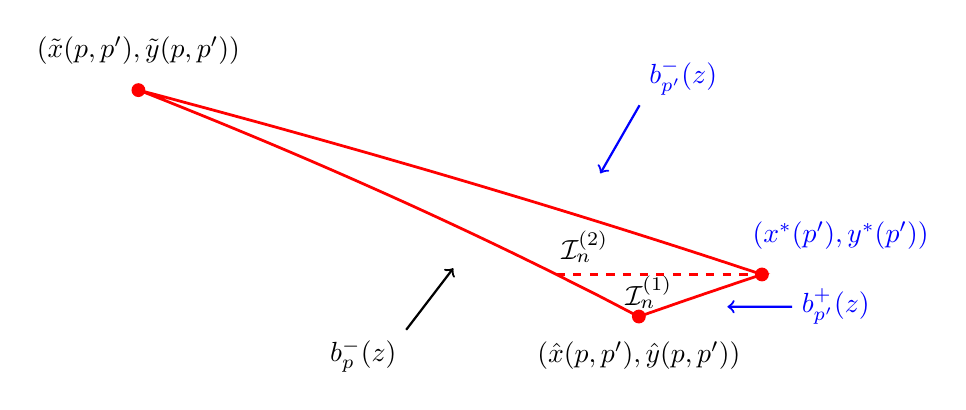
\begin{tikzpicture}[scale=5]

%%%%%%%%%%%%%%%%%%%%%%%%%%%%%%%%%%%%%%%%%%%%%%%%%%%%%%%%%%%%%%%%%%%%%%%%%%%%%%%%%%%%%%%%%%%%%%%%%%%
%																								  %
%	Shows the area T_{\Pcal \Delta \Pcal_n} when h(y) > h_1(p^\prime)							  %
%																								  %
%%%%%%%%%%%%%%%%%%%%%%%%%%%%%%%%%%%%%%%%%%%%%%%%%%%%%%%%%%%%%%%%%%%%%%%%%%%%%%%%%%%%%%%%%%%%%%%%%%%

	%Define the coordinates 
	%p = (\u,\v) and p^\prime = (\uu, \vv)
	%Box \Rcal has width 2\r and height \t
	\pgfmathsetmacro{\u}{0}
	\pgfmathsetmacro{\v}{1}
	\pgfmathsetmacro{\uu}{2.5}
	\pgfmathsetmacro{\vv}{1.8}
	\pgfmathsetmacro{\r}{6}
	\pgfmathsetmacro{\t}{4}
    
    %Define x^\ast(p^\prime) and y^\ast(p^\prime)
    \pgfmathsetmacro{\uuast}{\uu-\r}
    \pgfmathsetmacro{\vvast}{2*ln(\r)-\vv}
    
    %Define intersection left black and shifted blue curve
    \pgfmathsetmacro{\vast}{2*ln((2*\r - \uu)/(exp(\v/2) + exp(\vv/2)))}
    \pgfmathsetmacro{\uast}{(\uu - 2*\r)/(1 + exp((\vv - \v)/2))}    
    
    %Define intersection left black and left blue curve
    \pgfmathsetmacro{\utilde}{\uu/(1-exp((\vv-\v)/2))} 
    \pgfmathsetmacro{\vtilde}{2*ln(\uu-\utilde)-\vv}
   
    %Define h_1(p) = h_2(p)
    \pgfmathsetmacro{\hp}{2*ln(\r-\u)-\v}
    
    %Define h_1(p^\prime) and h_2(p^\prime)
    \pgfmathsetmacro{\hh}{2*ln(\uu+\r)-\vv}
    \pgfmathsetmacro{\hhh}{2*ln(\r-\uu)-\vv}
    
    %Draw the boundary left black, left blue and shifted right blue line
	\draw[red,line width=1pt] 
		plot[domain=\utilde:\uuast,smooth,variable=\x,red] (\x, {2*ln(\uu-\x)-\vv})
		--
		plot[domain=\uuast:\uast,smooth,variable=\x,red] (\x, {2*ln(\x+(2*\r-\uu))-\vv})
		--
		plot[domain=\uast:\utilde,smooth,variable=\x,red] (\x, {2*ln(-\x)-\v}); 
	
	%Calculate intersection point
	\pgfmathsetmacro{\i}{-exp((\v+\vvast)/2)}
	\draw[red, dashed,line width=1pt] (\i,\vvast) -- (\uuast,\vvast);

    \draw node at (\utilde,\vtilde+0.1) {\color{black}$(\tilde{x}(p,p^\prime), \tilde{y}(p,p^\prime))$};
    \draw node at (\uast,\vast-0.1) {$(\hat{x}(p,p^\prime), \hat{y}(p,p^\prime))$};
    \draw node at (\uuast+0.2,\vvast+0.1) {\color{blue}$(x^\ast(p^\prime), y^\ast(p^\prime))$};
   
    \draw node at (\uuast-0.45,\vvast+0.07) {$\mathcal{I}_n^{(2)}$};
    \draw node at (\uast+0.025,\vvast-0.045) {$\mathcal{I}_n^{(1)}$};
   
    \draw node (f1) at (\uast-0.7,\vast-0.1) {\color{black}$b_{p}^-(z)$};
    \draw node (f2) at (\uuast-0.2,\vvast+0.5) {\color{blue}$b_{p^\prime}^-(z)$};
    \draw node (f3) at (\uast+0.5,\vast+0.025) {\color{blue}$b_{p^\prime}^+(z)$};
    \path (f1)+(45:0.35) node (f1_arrow) {};
    \path (f2)+(230:0.35) node (f2_arrow) {};
    \path (f3)+(180:0.3) node (f3_arrow) {};
	\draw[->,thick] (f1.north east) -- (f1_arrow);
    \draw[->,thick,blue] (f2.south west) -- (f2_arrow);
    \draw[->,thick,blue] (f3.west) -- (f3_arrow);
%
	\draw node[red, fill, circle, inner sep=0pt, minimum size=5pt] at (\utilde,\vtilde) {};
	\draw node[red, fill, circle, inner sep=0pt, minimum size=5pt] at (\uast,\vast) {};
	\draw node[red, fill, circle, inner sep=0pt, minimum size=5pt] at (\uuast,\vvast) {};

\end{tikzpicture}
\caption{The different shapes of $\mathcal{T}_{\Pcal \Delta \Pcal_n}(p,p_1)$ depending on the regime to which $p_1$ belongs. The top figure is for $p_1 \in B_n^{(1)}$, the middle for $p_1 \in B_n^{(2)}$ and the bottom one for $p_1 \in B_n^{(3)}$.}
\label{fig:shapes_triangle_mismatches}
\end{figure}

\paragraph{Regime 1: $0 \le y_1 \le y - 2\log(I_n/(I_n-x_1))$}

In this case the integral over $p_2$ splits into two parts
\begin{align*}
	\mathcal{I}_n^{(1)}(p_1) &:= \int_{h_2(p_1)}^{y^\ast(p_1)} \int_{-I_n}^{x_1 + e^{(y_1+y_2)/2}-2I_n} e^{-\alpha y_2}
		\dd x_2 \dd y_2\\
	\mathcal{I}_n^{(2)}(p_1) &:= \int_{y^\ast(p_1)}^{h_1(p_1)} \int_{x^\ast(p_1)}^{x_1 - e^{(y_1+y_2)/2}} e^{-\alpha y_2}
		\dd x_2 \dd y_2.
\end{align*}

We first compute $\mathcal{I}_n^{(1)}$.
\begin{align*}
	\mathcal{I}_n^{(1)}(p_1) &= \int_{h_2(p_1)}^{y^\ast(p_1)} \left(x_1 + e^{(y_1+y_2)/2} - I_n\right) e^{-\alpha y_2} 
		\dd x_2 \dd y_2\\
	&\le e^{y_1/2} \int_{h_2(p_1)}^{y^\ast(p_1)} e^{-(\alpha-\frac{1}{2}) y_2} \dd y_2\\
	&= \frac{2 e^{y_1/2}}{2\alpha - 1} \left(e^{-(\alpha-\frac{1}{2})h_2(p_1)} - e^{-(\alpha-\frac{1}{2})y^\ast(p_1)}
		\right) \\
	&= \frac{2 e^{\alpha y_1}}{2\alpha - 1} I_n^{-(2\alpha -1)}\left(\left(1 - \frac{x_1}{I_n}\right)^{-(2\alpha - 1)}-1\right)\\
	&= \bigO{I_n^{-2\alpha} x_1 e^{\alpha y_1}},
\end{align*}
where we used that $x^\prime \le e^{(y+y_1)/2} = \smallO{I_n}$ for all $y_1\le y$ and $y \in \Kcal_{C}(k_n)$ so that
\[
	\left(\left(1 - \frac{x_1}{I_n}\right)^{-(2\alpha - 1)}-1\right) = \bigO{\frac{x^\prime}{I_n}} \quad 
	\text{as } n \to \infty.
\]

For $\mathcal{I}_n^{(2)}(p_1)$ we have
\begin{align*}
	\mathcal{I}_n^{(2)}(p_1) &= \int_{y^\ast(p_1)}^{h_1(p_1)} \left(I_n + x_1 - e^{(y_1+y_2)}\right) e^{-\alpha y_2}
		\dd x_2 \dd y_2\\
	&\le 2 I_n \int_{y^\ast(p_1)}^{h_1(p_1)} e^{-\alpha y_2} \dd x_2 \dd y_2\\
	&= \frac{2}{\alpha} I_n \left(I_n^{-2\alpha}e^{\alpha y_1} - \left(I_n + x_1\right)^{-2\alpha} e^{-\alpha y_1}\right)\\
	&= \bigO{I_n^{-2\alpha} x_1 e^{\alpha y_1}} = \bigO{I_n^{-(2\alpha - 1)} e^{\alpha y_1}}.
\end{align*}

We conclude that for $p_1 \in B_n^{(1)}$:
\[
	\mu\left(\mathcal{T}_{\Pcal \Delta \Pcal_n}(p,p_1)\right) = \bigO{I_n^{-2\alpha} x_1 e^{\alpha y_1}},
\]
which establishes the first part of \eqref{eq:mu_triangle_diff}.

\paragraph{Regime 2: $y - 2\log(I_n/(I_n-x_1)) < y_1 \le y + 2 \log\left(1 + \frac{x_1}{I_n}\right)$}

Here we split the integration into two parts (see Figure~\ref{fig:shapes_triangle_mismatches}). Recall that $x^\ast(p,p_1) = x_1 - I_n$. Then, for the first part we have
\begin{align*}
	\mathcal{I}_n^{(1)}(p,p_1) &\le \int_{h(y)}^{h_1(p_1)} \int_{-I_n}^{x^\ast(p,p_1)} f(x_2, y_2) 
		\dd x_2 \dd y_2\\
	&= \bigO{x_1 \left(e^{-\alpha h(y)} - e^{-\alpha h_1(p_1)}\right)}\\
	&= \bigO{x_1 I_n^{-2\alpha}\left(e^{\alpha y} - e^{\alpha y_1}\left(1 + \frac{x_1}{I_n}\right)^{-2\alpha}\right)}\\
	&= \bigO{I_n^{-2\alpha} x_1 e^{\alpha y_1}\left(\left(1 - \frac{x_1}{I_n}\right)^{-2\alpha} 
		- \left(1 + \frac{x_1}{I_n}\right)^{-2\alpha}\right)}\\
	&= \bigO{I_n^{-2\alpha} x_1 e^{\alpha y_1}} = \bigO{I_n^{-(2\alpha - 1)} e^{\alpha y}}, 
\end{align*}
were we used that $y \le y_1 + 2\log(I_n/(I_n-x_1))$ for $p_1 \in B_n^{(2)}$ for the third line and 
\[
	\left(1 - \frac{x_1}{I_n}\right)^{-2\alpha} - \left(1 + \frac{x_1}{I_n}\right)^{-2\alpha}
	= \bigO{\frac{x_1}{I_n}} = \bigO{1},
\]
for the last line.

For the second part we first compute that 
\begin{align*}
	x_1 + e^{(y_1+y_2)/2} - 2 I_n + e^{(y + y_2)/2} &\le \left(e^{y/2} + e^{y_1/2}\right)e^{y_2/2}\\
	&\le e^{y/2}\left(1 + \frac{I_n}{I_n - e^y}\right)e^{y_2/2} = \bigO{e^{(y+y_2)/2}},
\end{align*}
since $y \in \Kcal_{C}(k_n)$ and $k_n = \smallO{\sqrt{n}}$, so that $e^y = \smallO{n} = \smallO{I_n}$. 
Then we have
\begin{align*}
	\mathcal{I}_n^{(2)} &= \int_{\hat{y}(p,p_1)}^{h(y)} \int_{-e^{(y + y_2)/2}}^{x_1 + e^{(y+y_1)/2} - 2 I_n} 
		f(x_2, y_2) \dd x_2 \dd y_2\\
	&= \bigO{e^{y/2} \int_{\hat{y}(p,p_1)}^{h(y)} e^{-(\alpha -\frac{1}{2}) y_2} \dd y_2}\\
	&= \bigO{e^{y/2} \left(e^{-(\alpha -\frac{1}{2}) \hat{y}(p,p_1)} - e^{-(\alpha -\frac{1}{2}) h(y)}\right)}\\
	&= \bigO{e^{y/2} \left(\left(\frac{2I_n - x_1}{e^{y/2} + e^{y_1/2}}\right)^{-(2\alpha-1)} 
		- I_n^{-(2\alpha-1)} e^{(\alpha -\frac{1}{2}) y}\right)}\\
	&= \bigO{I_n^{-(2\alpha-1)} e^{\alpha y}},
\end{align*}
where for the last line we first used that $(2I_n - x_1)^{-(2\alpha-1)} \le I_n^{-(2\alpha-1)}$ and then
\[
	\left(\left(e^{y/2} + e^{y_1/2}\right)^{2\alpha-1}- e^{(\alpha -\frac{1}{2}) y}\right)
	\le e^{(\alpha -\frac{1}{2}) y}\left(\left(1 + \sqrt{1+\frac{x_1}{I_n}} \, \right)^{2\alpha - 1} - 1\right)
	= \bigO{e^{(\alpha -\frac{1}{2}) y}}.
\]

It then follows that for $p_1 \in B_n^{(2)}$
\[
	\mu\left(\mathcal{T}_{\Pcal \Delta \Pcal_n}(p,p_1)\right) = \bigO{I_n^{-(2\alpha-1)} e^{\alpha y}}.
\]

\paragraph{Regime III $\bm{p_1 \in B_n^{(3)}}$:}

\begin{align*}
	\mathcal{I}_n^{(1)} &= \int_{y^\ast}^{\tilde{y}} \int_{-e^{(y+y_2)/2}}^{x_1-e^{(y_1+y_2)/2}} f(x_2,y_2)
		\dd x_2 \dd y_2\\
	&= \bigO{\int_{y^\ast}^{\tilde{y}} x_1 e^{-\alpha y_2} - \left(e^{y_1/2} - e^{y/2}\right)e^{-(\alpha - \frac{1}{2})y_2}
		\dd y_2}\\
	&= \bigO{x_1 \int_{y^\ast}^{\tilde{y}}  e^{-\alpha y_2} \dd y_2}.
\end{align*}

Now 
\begin{align*}
	\int_{y^\ast}^{\tilde{y}}  e^{-\alpha y_2} \dd y_2 
	&= \frac{1}{\alpha}\left(e^{-\alpha y^\ast} - e^{-\alpha \tilde{y}}\right) 
		= \frac{1}{\alpha}\left(I_n^{-2\alpha} e^{\alpha y_1} 
		- \left(\frac{x_1}{e^{y_1/2} - e^{y/2}}\right)^{-2\alpha}\right) \\
	&= \frac{I_n^{-2\alpha} e^{\alpha y_1}}{\alpha}\left(1 - \left(1 - e^{(y - y_1)/2}\right)^{2\alpha}
		\left(\frac{x_1}{I_n}\right)^{-2\alpha}\right) = \bigO{I_n^{-2\alpha} e^{\alpha y_1}},
\end{align*}
and hence we have
\[
	\mathcal{I}_n^{(1)} = \bigO{I_n^{-2\alpha} x_1 e^{\alpha y_1}}.
\]

For the second integral we have
\begin{align*}
	\mathcal{I}_n^{(2)} &= \int_{\hat{y}}^{y^\ast} \int_{-e^{(y+y_2)/2}}^{e^{(y_1 + y_2)/2} + x_1 - 2I_n} 
		f(x_2,y_2)\dd x_2 \dd y_2\\
	&= \bigO{\int_{\hat{y}}^{y^\ast} \left(e^{y/2} + e^{y_1/2}\right)e^{-(\alpha - \frac{1}{2})y_2} \dd y_2}\\
	&= \bigO{ e^{y_1/2} \int_{\hat{y}}^{y^\ast}e^{-(\alpha - \frac{1}{2})y_2} \dd y_2}.
\end{align*}

For the integral we have
\begin{align*}
	\int_{\hat{y}}^{y^\ast}e^{-(\alpha - \frac{1}{2})y_2} \dd y_2
	&= \frac{2}{2\alpha - 1} \left(e^{-(\alpha - \frac{1}{2})\hat{y}} - e^{-(\alpha - \frac{1}{2})y^\ast}\right)\\
	&= \frac{2}{2\alpha - 1}\left(\left(\frac{2I_n - x_1}{e^{y/2} + e^{y_1/2}}\right)^{-(2\alpha - 1)} 
		- I_n^{-(2\alpha - 1)} e^{-(\alpha - \frac{1}{2})y_1}\right)\\
	&= \bigO{I_n^{-2\alpha} x_1 e^{-(\alpha - \frac{1}{2})y_1}}
\end{align*}
so that
\[
	\mathcal{I}_n^{(2)} = \bigO{I_n^{-(2\alpha - 1)} e^{(1-\alpha)y_1}} = \bigO{I_n^{-2\alpha} x_1 e^{\alpha y}}
\]
and hence for $p_1 \in B_n^{(3)}$
\[
	\mu\left(\mathcal{T}_{\Pcal \Delta \Pcal_n}(p,p_1)\right) = \bigO{I_n^{-2\alpha} x_1 e^{\alpha y}}
	= \bigO{I_n^{-(2\alpha - 1)} e^{\alpha y}}.
\]

\subsubsection*{Integration over $p_1$}



We now proceed with the second part of the computation leading to \eqref{eq:clustering_error_T_main}. Here we will integrate $\mu(\mathcal{T}_{\Pcal \Delta \Pcal_n})(p,p_1)$ over the region $B_n := B_n^{(1)} \cup B_n^{(2)} \cup B_n^{(3)}$, see Figure~\ref{fig:comparing_triangles_B_areas}. Let us first identify the boundaries of these areas. 

The area $B_n^{(1)}$ is bounded from above by the line given by the equation
\[
	y_1 = y - 2\log\left(\frac{I_n}{I_n - x_1}\right).
\]
Solving this for $x_1$ yields $x_1 = I_n\left(1 - e^{(y_1-y)/2}\right)$ and hence the area $B_n^{(1)}$ is given by
\[
	B_n^{(1)} = \left\{(x_1, y_1) \, : \, 0 \le y_1 \le y, \quad 0 \le x_1 \le I_n\left(1 - e^{(y_1-y)/2}\right) \wedge e^{(y + y_1)/2} \right\}.
\]

In a similar way we have that $B_n^{(2)}$ is bounded from above by line
\[
	y_1 = y + 2\log\left(\frac{I_n}{I_n + x_1}\right),
\]
which yields $x_1 = I_n\left(e^{(y_1 - y)/2} - 1\right)$. The lower red boundary is the upper boundary of $B_n^{(2)}$ and hence we have
\[
	B_n^{(2)} = \left\{(x_1, y_1) \, : \, h_\ast(y) \le y_1 \le h^\ast(y), \,\, I_n\left(1 - e^{(y_1-y)/2}\right) \vee 
	I_n\left(e^{(y_1 - y)/2} - 1\right) \le x_1 \le e^{(y + y_1)/2} \right\}.
\]

We continue is the same way to obtain for $B_n^{(3)}$
\[
	B_n^{(3)} = \left\{(x_1, y_1) \, : \, y \le y_1 \le R_n, \,\,
	I_n\left(1 - e^{(y - y_1)/2}\right) \le x_1 \le I_n\left(e^{(y_1 - y)/2} - 1\right) \wedge e^{(y + y_1)/2} \wedge I_n \right\}.
\]

We these characterizations of the areas we now integrate $\mu(\mathcal{T}_{\Pcal \Delta \Pcal_n})(p,p_1)$ over $B_n$, splitting the computations over the three different areas.

\paragraph{$\bm{p_1 \in B_n^{(1)}}:$}

We use that $I_n\left(1 - e^{(y_1-y)/2}\right) \wedge e^{(y + y_1)/2} \le I_n\left(1 - e^{(y_1-y)/2}\right)$ so that
\begin{align*}
	&\hspace{-30pt}\int_{B_n^{(1)}} \mu\left(\mathcal{T}_{\Pcal \Delta \Pcal_n}(p,p_1)\right) 
		f(x_1,y_1)	\dd x_1 \dd y_1 \\
	&\le  \int_0^y \int_0^{I_n(1-e^{(y_1-y)/2})} \mu\left(\mathcal{T}_{\Pcal \Delta \Pcal_n}(p,p_1)\right) 
		f(x_1,y_1) \dd x_1 \dd y_1\\
	&= \bigO{ I_n^{-2\alpha} \int_0^y \int_0^{e^{(y+y_1)/2}}  x_1 \dd x_1 \dd y_1 }\\
	&= \bigO{I_n^{-(2\alpha-1)} \int_0^y \left(1 - e^{(y_1-y)/2}\right)^2 \dd y_1} \\
	&= \bigO{I_n^{-(2\alpha - 1)} y} = \bigO{y n^{-(2\alpha - 1)}}.
\end{align*} 

\paragraph{$\bm{p_1 \in B_n^{(2)}}:$}

We will show that
\begin{equation}\label{eq:mu_triangle_diff_2}
	\mu(B_n^{(2)}) = \bigO{I_n^{-1} e^{(2-\alpha)y}},
\end{equation}
which together with \eqref{eq:mu_triangle_diff} yields
\begin{align*}
	\int_{B_n^{(2)}} \mu\left(\mathcal{T}_{\Pcal \Delta \Pcal_n}(p,p_1)\right) 
		f(x_1,y_1)	\dd x_1 \dd y_1
	&= \bigO{\mu(B_n^{(2)}) I_n^{-(2\alpha - 1)} e^{\alpha y}}\\
	&= \bigO{I_n^{-2\alpha} e^{2y}}.
\end{align*}

The integration is split into two parts determined by $I_n\left(1 - e^{(y_1-y)/2}\right) \vee 
	I_n\left(e^{(y_1 - y)/2} - 1\right)$:
\begin{align*}
	\mu(B_n^{(3)}) &= \int_{h_\ast(y)}^{y} \int_{I_n(1-e^{(y_1-y)/2})}^{e^{(y + y_1)/2}} 
		f(x_1,y_1) \dd x_1 \dd y_1\\
	&\hspace{10pt} + \int_y^{h^\ast(y)} \int_{I_n(e^{(y_1-y)/2}-1)}^{e^{(y + y_1)/2}} 
		f(x_1,y_1) \dd x_1 \dd y_1.
\end{align*}

For the first integral we use that $e^{(y + y_1)/2} - I_n(1-e^{(y_1-y)/2}) \le e^{y_1/2}\left(e^{y/2} + e^{-y/2}\right)$ to obtain
\begin{align*}
	&\hspace{-30pt}\int_{h_\ast(y)}^{y} \int_{I_n(1-e^{(y_1-y)/2})}^{e^{(y + y_1)/2}} f(x_1,y_1) 
		\dd x_1 \dd y_1\\
	&= \bigO{e^{y/2} \int_{h_\ast(y)}^{y} e^{-(\alpha - \frac{1}{2})y_1} \dd y_1}\\
	&= \bigO{e^{y/2}\left(e^{-(\alpha - \frac{1}{2})y} - e^{-(\alpha - \frac{1}{2})y} 
		\left(\frac{I_n}{I_n + e^y}\right)^{-(2\alpha - 1)}\right)}\\
	&= \bigO{I_n^{-1} e^{(2-\alpha)y}}.
\end{align*}
For the second integral note that $e^{(y + y_1)/2} - I_n(e^{(y_1-y)/2}-1) \le e^{(y + y_1)/2}$ and hence
\begin{align*}
	&\hspace{-30pt}\int_y^{h^\ast(y)} \int_{I_n(e^{(y_1-y)/2}-1)}^{e^{(y + y_1)/2}} f(x_1,y_1) 
		\dd x_1 \dd y_1\\
	&= \bigO{e^{y/2} \int_y^{h^\ast(y)} e^{-(\alpha - \frac{1}{2})y_1} \dd y_1}\\
	&= \bigO{e^{y/2} \left(e^{-(\alpha - \frac{1}{2})y} - e^{-(\alpha - \frac{1}{2})y}
		\left(\frac{I_n}{I_n - e^y}\right)^{-(2\alpha - 1)}\right)}\\
	&= \bigO{I_n^{-1} e^{(2-\alpha)y}},
\end{align*}
so that \eqref{eq:mu_triangle_diff_2} follows.

\paragraph{$\bm{p_1 \in B_n^{(3)}}:$}

For this area we show that 
\begin{equation}\label{eq:mu_triangle_diff_3}
	\mu(B_n^{(3)}) = \bigO{e^{(1-\alpha)y}}
\end{equation} 
so that
\begin{align*}
	\int_{B_n^{(3)}} \mu\left(\mathcal{T}_{\Pcal \Delta \Pcal_n}(p,p_1)\right) 
		f(x_1,y_1)	\dd x_1 \dd y_1
	&= \bigO{\mu(B_n^{(2)}) I_n^{-(2\alpha - 1)} e^{\alpha y}}\\
	&= \bigO{I_n^{-(2\alpha-1)} e^{y}}.
\end{align*}

Here the integral is split into three parts:
\begin{align*}
	\mu(B_n^{(3)}) &= \int_y^{h^\ast(y)} \int_{I_n(1-e^{(y-y_1)/2})}^{I_n(e^{(y_1-y)/2}-1)}
		f(x_1,y_1) \dd x_1 \dd y_1\\
	&\hspace{10pt}+ \int_{h^\ast(y)}^{h(y)} \int_{I_n(1-e^{(y-y_1)/2})}^{e^{(y+y_1)/2}}
		f(x_1,y_1) \dd x_1 \dd y_1\\
	&\hspace{10pt}+ \int_{h(y)}^{R_n} \int_{I_n(1-e^{(y-y_1)/2})}^{I_n}
		f(x_1,y_1) \dd x_1 \dd y_1.
\end{align*}

Let us first focus on the first integral. Since	$I_n(e^{(y_1-y)/2}-1) - I_n(1-e^{(y-y_1)/2}) \le I_n e^{(y_1-y)/2}$ we get,
using similar arguments as above
\begin{align*}
	\int_y^{h^\ast(y)} \int_{I_n(1-e^{(y-y_1)/2})}^{I_n(e^{(y_1-y)/2}-1)} f(x_1,y_1) \dd x_1 \dd y_1
	&= \bigO{I_n e^{-y/2} \int_y^{h^\ast(y)} e^{-(\alpha - \frac{1}{2})y_1} \dd y_1}\\
	&= \bigO{I_n e^{-\alpha y} \left(1 - \left(\frac{I_n}{I_n - e^y}\right)^{-(2\alpha - 1)}\right)}\\
	&= \bigO{e^{(1-\alpha)y}}.
\end{align*}

Proceeding to the second integral, we first note that $e^{(y+y_1)/2} - I_n(1-e^{(y-y_1)/2}) = \bigO{I_n e^{(y_1-y)/2}}$ so that similar calculations as before yield
\begin{align*}
	\int_{h^\ast(y)}^{h(y)} \int_{I_n(1-e^{(y-y_1)/2})}^{e^{(y+y_1)/2}}	f(x_1,y_1) \dd x_1 \dd y_1
	&= \bigO{I_n e^{-y/2} \int_{h^\ast(y)}^{h(y)} e^{-(\alpha - \frac{1}{2})y_1} \dd y_1}
		= \bigO{e^{(1-\alpha)y}}.
\end{align*}



\end{proof}

\section{Concentration for $c(k; \Gbox)$ (Proving Proposition \ref{prop:concentration_local_clustering_P_n})}
\label{sec:concentration_c_P_n}

In this section we establish a concentration result for the local clustering function $c^\ast(k; \Gbox)$ in the finite box model $\Gbox$. Similar to the previous section we will focus on typical points $p = (0,y)$ with $y \in \Kcal_{C}(k_n)$.

\subsection{The main contribution of triangles}

First we write
\[
	c^\ast(k_n ; \Gbox) = \frac{T_{\text{box}}(k_n)}{\binom{k_n}{2}\Exp{\Nbox(k_n)}},
\]
where
\[
	 T_{\text{box}}(k_n) = \sum_{p \in \Pcal} \ind{\Dbox(p) = k_n} \sum_{p_1, p_2 \in \Pcal \setminus p}^{\ne} 
	 \ind{p_1 \in \BallPon{p}}\ind{p_2 \in \BallPon{p}}\ind{p_2 \in \BallPon{p_1}}
\]
In particular, the variance of $c^\ast(k_n ; \Gbox)$ is determined by the variance of $T_{\text{box}}(k_n)$.

Next, recall the adjusted triangle count function
\[
	\widetilde{T}_{\text{box}}(p_0) = \sum_{(p_1, p_2) \in \Pcal \setminus p_0}^{\ne} 
		\widetilde{T}_{\text{box}}(p_0,p_1,p_2).
\]
where
\[
	\widetilde{T}_{\text{box}}(p_0,p_1,p_2) = \ind{p_1 \in \BallPon{p_0}}\ind{p_2 \in \BallPon{p_0}}\ind{p_2 \in \BallPo{p_1} \cap \Rcal},
\]
and recall the definition of $\Kcal_{C}(k_n)$
\[
	\Kcal_{C}(k_n) = \left\{y \in \R_+ : \frac{k_n - C \sqrt{k_n \log(k_n)}}{\xi} \vee 1 \le e^{\frac{y}{2}}
		\le \frac{k_n + C \sqrt{k_n \log(k_n)}}{\xi} \right\},
\]
and write $\Rcal(k_n,C) = [-I_n,I_n] \times \Kcal_{C}(k_n)$ for the part of the box $\Rcal$ with heights in $\Kcal_{C}(k_n)$.
Slightly abusing notation, we will define the corresponding triangle degree function
\begin{equation}\label{eq:def_degree_triangle_count_in_K}
	\widetilde{T}_{\text{box}}(k_n, C) = \sum_{p \in \Pcal \cap \Rcal(k_n,C)} \ind{\text{deg}_{\text{box}}(p) = k_n} \widetilde{T}_{\text{box}}(p).
\end{equation}
and with that a different clustering function.
\begin{equation}\label{eq:def_tilde_c_box}
	\widetilde{c}_{\text{box}}(k_n) = \frac{\widetilde{T}_{\text{box}}(k_n,C)}{\binom{k_n}{2}\Exp{N_{\text{box}}(k_n)}}
\end{equation}
The idea is that the main contribution of triangles of degree $k_n$ to the triangle count $T_{\text{box}}(k_n)$ is given by $\widetilde{T}_{\text{box}}(k_n, C)$. Therefore, in order to prove Proposition \ref{prop:concentration_local_clustering_P_n} it suffices to show that $\widetilde{T}_{\text{box}}(k_n,C)$ is sufficiently concentrated around its mean. This last part is done in the following proposition.

%\subsection{The proof of Proposition \ref{prop:concentration_local_clustering_P_n}}
%
%We start with the concentration result for $\widetilde{T}_{\text{box}}(k_n)$.

\begin{proposition}[Concentration $\widetilde{T}_{\text{box}}(k_n,C)$]\label{prop:concentration_tilde_T_P_n}
Let $\alpha > \frac{1}{2}$, $\nu > 0$ and let $(k_n)_{n \ge 1}$ be any positive sequence satisfying $k_n = \smallO{n^{\frac{1}{2\alpha+1}}}$. Then for any $C > 0$, as $n \to \infty$,
\[
	\Exp{\widetilde{T}_{\text{box}}(k_n,C)^2} = \left(1 + \smallO{1}\right)\Exp{\widetilde{T}_{\text{box}}(k_n, C)}^2.
\]
\end{proposition}

We first use this result to prove Proposition~\ref{prop:concentration_local_clustering_P_n}. The remainder of this section is devoted to prove Proposition~\ref{prop:concentration_tilde_T_P_n}. The final proof can be found in Section~\ref{ssec:concentration_tilde_T}.

\begin{proof}[Proof of Proposition \ref{prop:concentration_local_clustering_P_n}]
We bound the expectation as follows,
\begin{align*}
	\Exp{\left|c^\ast(k_n; \Gbox) - \Exp{c^\ast(k_n; \Gbox)}\right|} 
	&\le \frac{\Exp{\left|\widetilde{T}_{\text{box}}(k_n,C) - \Exp{\widetilde{T}_{\text{box}}(k_n,C)}\right|}}
		{\binom{k_n}{2}\Exp{N_{\text{box}}(k_n)}}\\
	&\hspace{10pt} + 2 \Exp{\left|c^\ast(k_n; \Gbox) - \widetilde{c}_{\text{box}}(k_n)\right|}.
\end{align*}
We will show that both terms are $\smallO{s(k_n)}$.

First we note that $\ind{p_2 \in \BallPo{p_1} \cap \Rcal} \le \ind{p_2 \in \BallPon{p_1}}$ and hence $\widetilde{T}_{\text{box}}(p) \le T_{\text{box}}(p)$. This implies that
\[
	 \widetilde{c}_{\text{box}}(k_n) = \frac{\widetilde{T}_{\text{box}}(k_n,C)}{\binom{k_n}{2}\Exp{N_{\text{box}}(k_n)}} \le c^\ast(k_n; \Gbox). 
\]
and therefore
\[
	\Exp{\left|c^\ast(k_n; \Gbox) - \widetilde{c}_{\text{box}}(k_n)\right|}
	= \Exp{c^\ast(k_n; \Gbox)} - \widetilde{c}_{\text{box}}(k_n).
\]
For the expectation of $\widetilde{T}_{\text{box}}(k_n,C)$ we use that 
\[
	\CExp{\widetilde{T}_{\text{box}}(p)}{\Dbox(p) = k_n}
= \binom{k_n}{2} \Mu{\BallPon{y}}^{-2} \Exp{\widetilde{T}_{\text{box}}(p)},
\] 
to get
\begin{align*}
	\Exp{\widetilde{T}_{\text{box}}(k_n,C)} 
	&= \int_{\Rcal(k_n,C)} \CExp{\widetilde{T}_{\text{box}}(p)}{\Dbox(p) = k_n}
		\rho_{\text{box}}(y,k_n) f(x,y) \dd x \dd y\\
	&= (1+\smallO{1}) \binom{k_n}{2} \int_{\Rcal(k_n,C)} \Mu{\BallPon{y}}^{-2} \Exp{\widetilde{T}_{\text{box}}(y)}
		\rho_{\text{box}}(y,k_n) \alpha e^{-\alpha y} \dd y\\
	&= (1+\smallO{1}) \frac{1}{2} \int_{\Rcal(k_n,C)} \Exp{\widetilde{T}_{\text{box}}(y)}
			\rho_{\text{box}}(y,k_n) \alpha e^{-\alpha y} \dd y\\
	&= (1+\smallO{1}) n \binom{k_n}{2} \int_0^\infty P(y) \rho(y,k_n) \alpha e^{-\alpha y} \dd y,
\end{align*}
where the last line is due to Corollary~\ref{cor:adjusted_triangle_counting_P_n}. In particular, since the last integral is $\bigT{k_n^{-(2\alpha + 1)} s(k_n)}$ we conclude that
\begin{equation}\label{eq:scaling_exected_tilde_T}
	\Exp{\widetilde{T}_{\text{box}}(k_n,C)} = \bigT{n k_n^{-(2\alpha - 1)}s(k_n)}. 
\end{equation}

Since $\Exp{N_{\text{box}}(k_n)} = (1+\smallO{1}n p_{k_n}$ it follows that
\[
	\widetilde{c}_{\text{box}}(k_n) = \frac{\Exp{\widetilde{T}_{\text{box}}(k_n,C)}}{\binom{k_n}{2}\Exp{N_{\text{box}}(k_n)}}
	= (1+\smallO{1}) \frac{\int_0^\infty P(y) \alpha e^{-\alpha y} \dd y}{p_{k_n}}
	= (1 + \smallO{1}) \gamma(k_n).
\]
On the other hand, Proposition~\ref{prop:convergence_average_clustering_P_n} implies that $\Exp{c^\ast(k_n; \Gbox)} = (1+\smallO{1})\gamma(k_n)$ and thus we conclude that
\[
	2\Exp{\left|c^\ast(k_n; \Gbox) - \widetilde{c}_{\text{box}}(k_n)\right|}
	= \smallO{\gamma(k_n)} = \smallO{s(k_n)}.	
\]

For the remaining term we use H\"{o}lder's inequality and Proposition \ref{prop:concentration_tilde_T_P_n} to obtain
\begin{align*}
	\Exp{\left|\widetilde{T}_{\text{box}}(k_n,C) - \Exp{\widetilde{T}_{\text{box}}(k_n,C)}\right|}
	&\le \left(\Exp{\widetilde{T}_{\text{box}}(k_n,C)^2} 
		- \Exp{\widetilde{T}_{\text{box}}(k_n,C)}^2\right)^{\frac{1}{2}}\\
	&= \smallO{\Exp{\widetilde{T}_{\text{box}}(k_n,C)}}.
\end{align*}
This implies
\begin{align*}
	\frac{\Exp{\left|\widetilde{T}_{\text{box}}(k_n,C) - \Exp{\widetilde{T}_{\text{box}}(k_n,C)}\right|}}
		{\binom{k_n}{2}\Exp{N_{\text{box}}(k_n)}}
	&= \smallO{\frac{\Exp{\widetilde{T}_{\text{box}}(k_n,C)}}{\binom{k_n}{2}\Exp{N_{\text{box}}(k_n)}}}
	= \smallO{s(k_n)},
\end{align*}
which finishes the proof.
\end{proof}

We note that the above proof establishes the following important result

\begin{corollary}\label{cor:c_ast_box_2_tilde_c_box}
Let $k_n \to \infty$. Then, as $n \to \infty$,
\[
	\Exp{\left|c^\ast(k_n; \Gbox) - \widetilde{c}_{\text{box}}(k_n)\right|} = \smallO{s(k_n)}.
\]
\end{corollary}

\subsection{Joint neighborhoods and degrees in $\Gbox$}

To prove Proposition~\ref{prop:concentration_tilde_T_P_n} we need to understand the joint degree distribution in $\Gbox$. This subsequently requires us to compute the joint neighborhoods in $\Gbox$ of two points $p, p^\prime \in \Rcal$. We perform the analysis in this section. We start with a general result for near independent Poisson random variables.

\begin{lemma}\label{lem:near_independence_poisson}
Let $k_n \to \infty$ and $X_1 = \Po(\lambda_1(n))$, $X_2 = \Po(\lambda_2(n))$ and $Y = \Po(\lambda_3(n))$, be three Poisson random variables where $\lambda_3(n) = \bigO{k_n^{1-\varepsilon}}$, for some $0 < \varepsilon < 1$ and for some $C > 0$,
\[
	k_n - C\sqrt{k_n \log(k_n)} \le \lambda_i(n) + \lambda_3(n) \le k_n + C\sqrt{k_n \log(k_n)},
\] 
for $i = 1,2$.Then, as $n \to \infty$
\[
	\Prob{X_1 + Y = k_n, X_2 + Y = k_n} = (1+\smallO{1}) \Prob{X_1 + Y = k_n}\Prob{X_2 + Y = k_n}.
\]
\end{lemma}

\begin{proof}
First we write
\begin{align*}
	\Prob{X_1 + Y = k_n, X_2 + Y = k_n} 
	&= \sum_{t = 0}^\infty \Prob{X_1 = k_n - t}\Prob{X_2 = k_n - t}\Prob{Y = t}.
\end{align*}
Now fix a $C_1 > 0$ and define the set
\[
	A_n := \left\{t \in \R_+ \, : \, \lambda_3(n) - C_1\sqrt{k_n^{1-\varepsilon}\log(k_n)} \le t 
	\le \lambda_3(n) + C_1\sqrt{k_n^{1-\varepsilon}\log(k_n)} \right\}.
\]
Then by a Chernoff bound (c.f. \eqref{eq:def_chernoff_bound_poisson})
\begin{align*}
	&\hspace{-20pt}\sum_{t \in \R_+ \setminus A_n} \Prob{X_1 = k_n - t}\Prob{X_2 = k_n - t}\Prob{Y = t}\\
	&\le \Prob{Y > \lambda_3(n) + C_1\sqrt{k_n^{1-\varepsilon}\log(k_n)}} 
		+ \Prob{Y < \lambda_3(n) - C_1\sqrt{k_n^{1-\varepsilon}\log(k_n)}}\\
	&= \Prob{\left|\Po(\lambda_3(n)) - \lambda_3(n)\right| > C_1\sqrt{k_n^{1-\varepsilon}\log(k_n)}} 
		\le 2 k_n^{-\frac{C_1}{4}}.
\end{align*}
and hence
\[
	\Prob{X_1 + Y = k_n, X_2 + Y = k_n} 
	= \sum_{t \in A_n} \Prob{X_1 = k_n - t}\Prob{X_2 = k_n - t}\Prob{Y = t} + \bigO{k_n^{-(1+C_1^2)/2}}.
\]
Next, for $i=1,2$ we have by assumption on $\lambda_i(n) + \lambda_3(n)$ that
\begin{align*}
	\Prob{X_i + Y = k_n} &\ge \frac{\left(k_n + C\sqrt{k_n \log(k_n)}\right)^{k_n}}{k_n!} 
		e^{-\left(k_n + C\sqrt{k_n \log(k_n)}\right)}\\
	&\ge e^{-1} k_n^{-1/2} \left(1 + C\sqrt{\frac{\log(k_n)}{k_n}}\right)^{k_n} e^{-C\sqrt{k_n \log(k_n)}}\\
	&\ge e^{-1} k_n^{-1/2} e^{k_n \log\left(1 + C\sqrt{\frac{\log(k_n)}{k_n}}\right) -C\sqrt{k_n \log(k_n)}}\\
	&\ge e^{-1} k_n^{-1/2} e^{ -\frac{C^2}{2} \log(k_n)} = e^{-1} k_n^{-\frac{1+C^2}{2}}.
\end{align*}
where we also used that $\log(1+x) \ge x - x^2/2$, for $0\le x \le 1$ and $k_n! \ge e \sqrt{k_n} k_n^{k_n} e^{-k_n}$. Hence, by taking $C_1 > 4(1 + C^2)$ we get that $k_n^{-\frac{C_1}{4}} = \smallO{\Prob{X_1 + Y = k_n}\Prob{X_1 + Y = k_n}}$. It remains to show that 
\begin{align*}
	&\hspace{-20pt}\sum_{t \in A_n} \Prob{X_1 = k_n - t}\Prob{X_2 = k_n - t}\Prob{Y = t}\\
	&= (1 + \smallO{1}) \Prob{X_1 + Y = k_n} \Prob{X_2 + Y = k_n},
\end{align*}

For this take any $s \in A_n$ so that $|t-s| \le 2 C_1 \sqrt{k_n^{1-\varepsilon}\log(k_n)}$ and note that there exists a $\delta_n$ satisfying $|\delta_n| \le 2C \sqrt{k_n \log(k_n)}$, for $n$ large enough, such that $k_n - t = \lambda_1(n) + \delta_n$. It then follows that, uniformly in $t,s$ and $\delta_n$, as $n \to \infty$
\begin{align*}
	\frac{\Prob{X_2 = k_n - t}}{\Prob{X_2 = k_n - s}}
	&= \frac{\Prob{X_2 = k_n - t}}{\Prob{X_2 = k_n - t - (s - t)}}\\
	&= \frac{(k_n - t - (s-t))!}{(k_n - t)!} \lambda_1(n)^{s - t} \\
	&\sim (k_n - t - (s-t))^{-(s-t)} \lambda_1(n)^{s-t} \\
	&= \left(\lambda_1(n) + \delta_n - (s-t)\right)^{-(s-t)}\lambda_1(n)^{s-t}\\
	&= \left(1 + \frac{\delta_n -(s-t)}{\lambda_1(n)}\right)^{s-t}\\
	&\sim e^{\frac{(s-t)\delta_n}{\lambda_1(n)}} e^{-\frac{(s-t)^2}{\lambda_1(n)}} \sim 1,
\end{align*}
where the last line follows since both $\frac{(s-t)\delta_n}{\lambda_1(n)} \to 0$ and $\frac{(s-t)^2}{\lambda_1(n)} \to 0$ as $n \to \infty$. In particular,
\[
	\Prob{X_2 = k_n - t} = (1+\smallO{1}) \Prob{X_2 = k_n - s},
\] 
uniformly for all $t, s \in A_n$ and therefore, since
\[
	1 = \sum_{s = 0}^\infty \Prob{Y = s} = (1+\smallO{1}) \sum_{s \in A_n} \Prob{Y = s},
\]
we conclude that
\begin{align*}
	&\hspace{-20pt}\sum_{t \in A_n} \Prob{X_1 = k_n - t}\Prob{X_2 = k_n - t}\Prob{Y = t}\\
	&= (1+\smallO{1}) \sum_{t \in A_n} \Prob{X_1 = k_n - t}\Prob{X_2 = k_n - t}\Prob{Y = t} \sum_{s \in A_n} \Prob{Y = s}\\
	&= (1 + \smallO{1}) \sum_{t \in A_n} \Prob{X_1 = k_n - t}\Prob{Y = t} 
		\sum_{s \in A_n} \Prob{X_2 = k_n - s} \Prob{Y = s}\\
	&= (1 + \smallO{1}) \Prob{X_1 + Y = k_n} \Prob{X_2 + Y = k_n},
\end{align*}
from which the result follows.
\end{proof}

To see how this lemma can be applied to analyze the joint degree distribution in $\Gbox$, fix two points $p,p^\prime \in \Rcal$ and denote by 
\[
	\rho_{\text{box}}(p,p^\prime,k,k^\prime) 
	:= \Prob{\Po\left(\Mu{\BallPon{p}}\right) = k, \Po\left(\Mu{\BallPon{p^\prime}}\right) = k^\prime}.
\]
the joint degree distribution. Then if we define,
\begin{align*}
	X_1(p,p^\prime) &:= \Po\left(\Mu{\BallPon{p}\setminus \BallPon{p^\prime}}\right),\\
	X_2(p,p^\prime) &:= \Po\left(\Mu{\BallPon{p^\prime}\setminus \BallPon{p}}\right),\\
	Y(p,p^\prime) &:= \Po\left(\Mu{\BallPon{p} \cap \BallPon{p^\prime}}\right)
\end{align*}
it follows that
\[
	\rho_{\text{box}}(p,p^\prime,k_n,k_n) = \Prob{X_1(p,p^\prime) + Y(p,p^\prime) = k_n, X_2(p,p^\prime) + Y(p,p^\prime) = k_n}.
\]
Now, if $y,y^\prime \in \Kcal_{C}(k_n)$ the three Poisson random variables defined above satisfy the condition of Lemma~\ref{lem:near_independence_poisson} regarding the sum $\lambda_i(n) + \lambda_3(n)$. Therefore, if in addition $\Mu{\BallPon{p} \cup \BallPon{p^\prime}} = \bigO{k_n^{1-\varepsilon}}$, for some $0 < \varepsilon < 1$, we have that 
\[
	\rho_{\text{box}}(p,p^\prime,k_n,k_n) = (1+\smallO{1})\rho_{\text{box}}(p,k_n)\rho_{\text{box}}(p^\prime,k_n). 
\]

To make this more precise, we define, for any $0 < \varepsilon < 1$, the following set
\begin{equation}\label{eq:def_joint_degree_set_E_growing_k}
	\mathcal{E}_{\varepsilon}(k_n) = \left\{(p,p^\prime) \in \Rcal \times \Rcal
		\, : \, y,y^\prime \in \Kcal_{C}(k_n) \text{ and } |x - x^\prime| > k_n^{1 + \varepsilon} \right\}. 
\end{equation}
We will show (see Corollary~\ref{cor:expected_common_neighbors_Ecal_set}) that for all $(p,p^\prime) \in \mathcal{E}_\varepsilon(k_n)$ it holds that $\Mu{\BallPon{p} \cap \BallPon{p^\prime}} = \bigO{k_n^{1-\varepsilon}}$ and hence the joint degree distribution factorizes on this set. We will use this set later in Section~\ref{ssec:concentration_tilde_T} to prove Proposition~\ref{prop:concentration_tilde_T_P_n}. The main idea behind the above result is that if $p$ and $p^\prime$ are sufficiently separated in the $x$-direction, then the overlap of their neighborhoods $\BallPon{p} \cap \BallPon{p^\prime}$ is of smaller order than $\Mu{\BallPon{p}} + \Mu{\BallPon{p^\prime}}$. We shall therefore proceed with analyzing the joint neighborhoods in $\Gbox$.
%
%
%The following result shows that for any two points in the set
%
%The two main results, which will be the crucial technical ingredients for the proof of Proposition~\ref{prop:concentration_tilde_T_P_n}, are Lemma~\ref{lem:joint_degree_factorization} and Lemma~\ref{lem:joint_degree_distribution_shift}.

\subsubsection*{Joint neighborhoods}

Let $p, p^\prime \in \Rcal$ and denote by
%Then we denote by $\Ncal_{\text{box}}(p\Delta p^\prime)$ the number of disjoint neighbors of $p$ and $p^\prime$ in $\Gbox$, i.e. those points that belong to either $\BallPon{p}$ or $\BallPon{p^\prime}$ but not to their intersection. In addition we denote by 
$\Ncal_{\text{box}}(p,p^\prime)$ the number of joint neighbors of $p$ and $p^\prime$. We shall establish an upper bound on the expected number of joint neighbors when $p$ and $p6\prime$ are sufficiently separated. Observe that $\Exp{\Ncal_{\text{box}}(p,p^\prime)} = \Mu{\BallPon{p} \cap \BallPon{p^\prime}}$. 

%as well as an asymptotic expression for the expected number points in the joint neighborhood. For this we will distinguish between the cases where the distance between the $x$-coordinates of $p$ and $p^\prime$ is small or large. Figure~\ref{fig:representation_disjoint_neighborhoods_P_n}-\ref{fig:representation_disjoint_neighborhoods_P_n_3} show the different situations that occur.
%
%\begin{figure}[p]
%\centering
%\begin{tikzpicture}
%	
%	%The box \Rcal
%	\draw[line width=1pt] (-6,0) -- (6,0) -- (6,4) -- (-6,4) -- (-6,0);
%
%    \draw node[fill, circle, inner sep=0pt, minimum size=5pt] at (0,1) {};
%    \draw node at (-0.2,0.7) {$p$};
%    
%    \draw node[fill,blue, circle, inner sep=0pt, minimum size=5pt] at (1,0.5) {};
%    \draw node at (0.8,0.2) {\color{blue}$p^\prime$};
%	
%	\draw[domain=1.6487:6,smooth,variable=\x,black,line width=1pt] plot (\x, {2*ln(\x)-1});
%    \draw[domain=-1.6487:-6,smooth,variable=\x,black,line width=1pt] plot (\x, {2*ln(-\x)-1});
%    \draw[domain=2.2840:6,smooth,variable=\x,blue,line width=1pt] plot (\x, {2*ln(\x-1)-0.5});
%    \draw[domain=-0.2840:-6,smooth,variable=\x,blue,line width=1pt] plot (\x, {2*ln(1-\x)-0.5});
%    
%    \draw[dashed,thick,black,line width=1pt] (-6,2.5835) -- (6,2.5835);
%    
%    \draw node at (-7,2.5835) {$h(y)$};
%    \draw node at (-7,3.3918) {\color{blue}$h_1(p^\prime)$};
%    \draw node at (7,2.7189) {\color{blue}$h_2(p^\prime)$};
%    
%    \draw node at (-4,3.5) {\color{blue}$x_1 = x^\prime - e^{\frac{y^\prime + y_1}{2}}$};
%    \draw node at (4.5,3) {\color{blue}$x_1 = x^\prime + e^{\frac{y^\prime + y_1}{2}}$};
%    \draw node at (-4.5,1) {$x_1 = x - e^{\frac{y + y_1}{2}}$};
%    \draw node at (2,1.5) {$x_1 = x + e^{\frac{y + y_1}{2}}$};
%
%\end{tikzpicture}
%\caption{Schematic representation of the neighborhoods of $p$ and $p^\prime$ in $\Gbox$ when $|x-x^\prime| \le e^{\frac{y + y^\prime}{2}}$ used for the proof of Lemma~\ref{lem:disjoint_neighbors_P_n} and Lemma~\ref{lem:common_neighbors_Pcal_n}.}
%\label{fig:representation_disjoint_neighborhoods_P_n}
%\end{figure}~
%\begin{figure}[p]
%\centering
%\begin{tikzpicture}
%	
%	%The box \Rcal
%	\draw[line width=1pt] (-6,0) -- (6,0) -- (6,4) -- (-6,4) -- (-6,0);
%
%    \draw node[fill, circle, inner sep=0pt, minimum size=5pt] at (0,1) {};
%    \draw node at (-0.2,0.7) {$p$};
%    
%    \draw node[fill,blue, circle, inner sep=0pt, minimum size=5pt] at (2.5,0.5) {};
%    \draw node at (2.3,0.2) {\color{blue}$p^\prime$};
%	
%	\draw[domain=1.6487:6,smooth,variable=\x,black,line width=1pt] plot (\x, {2*ln(\x)-1});
%    \draw[domain=-1.6487:-6,smooth,variable=\x,black,line width=1pt] plot (\x, {2*ln(-\x)-1});
%    \draw[domain=3.7840:6,smooth,variable=\x,blue,line width=1pt] plot (\x, {2*ln(\x-2.5)-0.5});
%    \draw[domain=1.2160:-6,smooth,variable=\x,blue,line width=1pt] plot (\x, {2*ln(2.5-\x)-0.5});
%    \draw[domain=0:-6,smooth,variable=\x,blue,line width=1pt] plot (\x, {2*ln(\x+9.5)-0.5});
%    
%    \draw[dashed,black,line width=1pt] (-6,2.0055) -- (6,2.0055);
%    
%%    \draw node at (-7,2.5835) {$h(y)$};
%    \draw node at (-7,3.7801) {\color{blue}$h_1(p^\prime)$};
%    \draw node at (7,2.0055) {\color{blue}$h_2(p^\prime)$};
%    
%%    \draw[dotted,thick,black] (4.5208,2.0174) -- (4.5208,0);
%%    \draw[dotted,thick,black] (4.5208,2.0174) -- (6,2.0174);
%    
%%    \draw node at (4.5208,-0.5) {$w_x(p,p^\prime)$};
%%    \draw node at (7,2.0174) {$w_y(p,p^\prime)$};
%    
%    \draw node at (0,3.5) {\color{blue}$x_1 = x^\prime + e^{\frac{y^\prime + y_1}{2}}$};
%    \draw node at (-2,1.6) {\color{blue}$x_1 = x^\prime - e^{\frac{y^\prime + y_1}{2}}$};
%    \draw node at (-4.5,1) {$x_1 = x - e^{\frac{y + y_1}{2}}$};
%    \draw node at (2,1.5) {$x_1 = x + e^{\frac{y + y_1}{2}}$};
%
%\end{tikzpicture}
%\caption{Schematic representation of the neighborhoods of $p$ and $p^\prime$ in $\Gbox$ when $e^{\frac{y + y^\prime}{2}} < |x - x^\prime| \le e^{\frac{y}{2}} + e^{\frac{y^\prime}{2}}$ used for the proof of Lemma~\ref{lem:disjoint_neighbors_P_n} and Lemma~\ref{lem:common_neighbors_Pcal_n}.}
%\label{fig:representation_disjoint_neighborhoods_P_n_2}
%\end{figure}~

\begin{figure}[!ht]
\centering
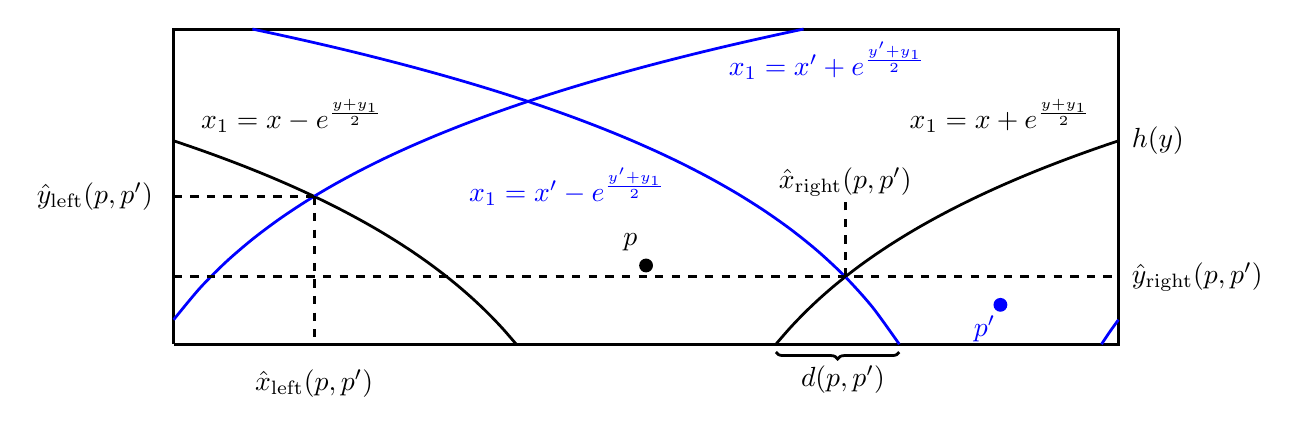
\begin{tikzpicture}
	

	\pgfmathsetmacro{\u}{0} %0
	\pgfmathsetmacro{\v}{1} %1
	\pgfmathsetmacro{\uu}{4.5} %1.4
	\pgfmathsetmacro{\vv}{0.5} %0.8
	\pgfmathsetmacro{\r}{6}
	\pgfmathsetmacro{\t}{4}
	
	%The box \Rcal
	\draw[line width=1pt] (-\r,0) -- (\r,0) -- (\r,\t) -- (-\r,\t) -- (-\r,0);
	
    \draw node[fill, circle, inner sep=0pt, minimum size=5pt] at (\u,\v) {};
    \draw node at (-0.2,1.3) {$p$};
    
    \draw node[fill,blue, circle, inner sep=0pt, minimum size=5pt] at (\uu,\vv) {};
    \draw node at (4.3,0.2) {\color{blue}$p^\prime$};
	
	\draw[domain=1.6487:6,smooth,variable=\x,black,line width=1pt] plot (\x, {2*ln(\x)-1});
    \draw[domain=-1.6487:-6,smooth,variable=\x,black,line width=1pt] plot (\x, {2*ln(-\x)-1});
    \draw[domain=5.7840:6,smooth,variable=\x,blue,line width=1pt] plot (\x, {2*ln(\x-4.5)-0.5});
    \draw[domain=3.2160:-5,smooth,variable=\x,blue,line width=1pt] plot (\x, {2*ln(4.5-\x)-0.5});
    \draw[domain=2:-6,smooth,variable=\x,blue,line width=1pt] plot (\x, {2*ln(\x+7.5)-0.5});
    
    
    
    \draw [decorate,decoration={brace},line width=1pt] (3.2160,-0.1) -- (1.6487,-0.1);
    \draw node at (2.5,-0.45) {$d(p,p^\prime)$};
    
%    \draw [dotted,line width=1pt] (2.5298,0.8563) -- (2.5298,1.7);
%    \draw node at (2.5298,2) {$\hat{x}(p,p^\prime)$};
    
    %Define intersection left black and shifted blue curve
    \pgfmathsetmacro{\vast}{2*ln((2*\r - \uu)/(exp(\v/2) + exp(\vv/2)))}
    \pgfmathsetmacro{\uast}{(\uu - 2*\r)/(1+exp((\vv-\v)/2))}
    %Define intersection right black and left blue curve
    \pgfmathsetmacro{\vvast}{2*ln((\uu)/(exp(\v/2) + exp(\vv/2)))}
    \pgfmathsetmacro{\uuast}{(\u*exp(\vv/2) + \uu*exp(\v/2))/(exp(\v/2) + exp(\vv/2))}
    \pgfmathsetmacro{\h}{2*ln(\r)-\v}
%    \draw[dotted,thick,black] (4.5208,2.0174) -- (4.5208,0);
%    \draw[dotted,thick,black] (4.5208,2.0174) -- (6,2.0174);
    
%    \draw node at (4.5208,-0.5) {$w_x(p,p^\prime)$};
%    \draw node at (7,2.0174) {$w_y(p,p^\prime)$};
    
    \draw node at (\r+0.5,\h) {$h(y)$};
    
    \draw node at (2.3,3.6) {\color{blue}$x_1 = x^\prime + e^{\frac{y^\prime + y_1}{2}}$};
    \draw node at (-1,2) {\color{blue}$x_1 = x^\prime - e^{\frac{y^\prime + y_1}{2}}$};
    \draw node at (-4.5,2.9) {$x_1 = x - e^{\frac{y + y_1}{2}}$};
    \draw node at (4.5,2.9) {$x_1 = x + e^{\frac{y + y_1}{2}}$};
	
	
	\draw[dashed,black,line width=1pt] (-\r,\vast) -- (\uast,\vast);
	\draw node at (-\r-1,\vast) {\color{black}$\hat{y}_{\text{left}}(p,p^\prime)$};
	\draw[dashed,line width=1pt] (\uast,\vast) -- (\uast,0);
	\draw node at (\uast,-0.5) {$\hat{x}_{\text{left}}(p,p^\prime)$};

	\draw[dashed,black,line width=1pt] (-\r,\vvast) -- (\r,\vvast);
	\draw node at (\r+1,\vvast) {\color{black}$\hat{y}_{\text{right}}(p,p^\prime)$};
	\draw[dashed,line width=1pt] (\uuast,\vvast) -- (\uuast,\vvast+1);
	\draw node at (\uuast,\vvast+1.2) {$\hat{x}_{\text{right}}(p,p^\prime)$};
	
	
\end{tikzpicture}
\caption{Schematic representation of the neighborhoods of $p$ and $p^\prime$ in $\Gbox$ when $|x - x^\prime| > e^{\frac{y}{2}} + e^{\frac{y^\prime}{2}}$ used for the proof of Lemma \ref{lem:disjoint_neighbors_P_n_large}. Note that although here $p^\prime \notin \BallPon{p}$, this is not true in general. This situation was merely chosen to improve readability of the figure.}
\label{fig:representation_disjoint_neighborhoods_P_n_3}
\end{figure}


We start by analyzing the shape of joint neighborhood. Due to symmetry and the fact that we have identified the left and right boundaries of the box $\Rcal$, we can, without loss of generality, assume that $p = (0,y)$ and $p^\prime = (x^\prime,y^\prime)$ with $x^\prime > 0$. To understand the computation it is helpful to have a picture. Figure~\ref{fig:representation_disjoint_neighborhoods_P_n_3} shows such an example. There are several different quantities that are important. The first are the heights where the left and right boundaries of the ball $\BallPon{p}$ go outside the box $\Rcal$. Since $x = 0$ these heights are the same and we denote this by $h(y)$. We also need to know the coordinates $\hat{y}_{\text{right}}(p,p^\prime)$ and $\hat{x}_{\text{right}}(p,p^\prime)$ of the intersection of the right boundary of the neighborhood of $p$ with the left boundary of the neighborhood of $p^\prime$ and those for the intersection of the left boundary of the neighborhood of $p$ with the right boundary of the neighborhood of $p^\prime$, which we denote by $\hat{y}_{\text{left}}(p,p^\prime)$ and $\hat{x}_{\text{left}}(p,p^\prime)$. Finally we will denote by $d(p,p^\prime)$ the distance between the lower right boundary of $\BallPon{p}$ and the lower left of $\BallPon{p^\prime}$, which is positive only when the bottom parts of both neighborhoods do not intersect, as is the case in Figure~\ref{fig:representation_disjoint_neighborhoods_P_n_3}. The condition $d(p,p^\prime) > 0$ is exactly the right notion for $p$ and $p^\prime$ being sufficiently separated.

Note that $\hat{y}_{\text{left}}(p,p^\prime)$ and $\hat{x}_{\text{left}}(p,p^\prime)$ correspond to, respectively, $\hat{y}(p,p^\prime)$ and $\hat{x}(p,p^\prime)$ considered in Section~\ref{ssec:missing_triangles}. The derivation of $\hat{y}_{\text{right}}(p,p^\prime)$ and $\hat{x}_{\text{right}}(p,p^\prime)$ is done in a similar manner and we omit the details here. The full expressions of all these functions are given below for further reference.

\begin{align}
	h(y) &= R_n - y + 2\log\left(\frac{\pi}{2}\right) \label{eq:def_height_y_P_n}\\
	h_1(p^\prime) &= 2\log\left(x^\prime + \frac{\pi}{2}e^{\frac{R_n}{2}}\right) - y^\prime \label{eq:def_height_left_P_n} \\
	h_2(p^\prime) &= 2\log\left(\frac{\pi}{2}e^{\frac{R_n}{2}} - x^\prime\right) - y^\prime 
		\label{eq:def_height_right_P_n} \\
%	\iota_x(p,p^\prime) &= \frac{(x^\prime-x)e^{\frac{y}{2}}}{e^{\frac{y}{2}} - e^{\frac{y^\prime}{2}}}
%		\label{eq:def_x_intersection_close_boundaries}\\
%	\iota_y(p,p^\prime) &= 2\log\left(\frac{x^\prime - x}{e^{\frac{y}{2}} - e^{\frac{y^\prime}{2}}}\right)
%		\label{eq:def_y_intersection_close_boundaries}\\
	\hat{y}_{\text{right}}(p,p^\prime) &= 2\log\left(\frac{x^\prime}{e^{\frac{y}{2}} + e^{\frac{y^\prime}{2}}}\right)\\
	\hat{x}_{\text{right}}(p,p^\prime) &= \frac{x^\prime}{1 + 	
		e^{\frac{y^\prime - y}{2}}},\\
	\hat{y}_{\text{left}}(p,p^\prime) &= 2 \log\left(\frac{\pi e^{R_n/2} - x^\prime}{e^{y/2} + e^{y^\prime/2}}\right),\\
	\hat{x}_{\text{left}}(p,p^\prime) &= \frac{x^\prime - \pi e^{R_n/2}}{1 + e^{\frac{y^\prime - y}{2}}}, \\
	d(p,p^\prime) &= |x - x^\prime| - \left(e^{\frac{y}{2}} + e^{\frac{y^\prime}{2}}\right).
	\label{eq:def_d_p_p_prime}
\end{align}

%We start with the result for points whose $x$-coordinates are close, which is when $d(p,p^\prime) < 0$.
%
%\begin{lemma}\label{lem:disjoint_neighbors_P_n}
%Let $p, p ^\prime \in \Rcal$ and denote $y^\ast = \min\{y, y^\prime\}$. Then whenever $|x - x^\prime| \le e^{\frac{y}{2}} + e^{\frac{y^\prime}{2}}$,
%\begin{align*}
%	\Exp{\Ncal_{\text{box}}(p \Delta p^\prime)}
%	&\ge \frac{\nu}{\pi}|x^\prime - x|\left(1 - \left(\frac{2}{\pi}\right)^{2\alpha}e^{-\alpha(R_n - y^\ast)}\right)\\
%	&\hspace{10pt}+ \xi\left|e^{\frac{y}{2}} - e^{\frac{y^\prime}{2}}\right|
%		\left(1 - \left(\frac{2}{\pi}\right)^{2\alpha - 1}e^{-(\alpha - \frac{1}{2})(R_n-y^\ast)}\right).
%\end{align*}
%\end{lemma}
%
%\begin{proof}
%In order to proof the result we will consider the area in between the two left boundaries of the balls $\BallPon{p}$ and
%$\BallPon{p^\prime}$ up to the height $h^\ast := \min\{h(y), h_2(p^\prime)\}$, see Figure~\ref{fig:representation_disjoint_neighborhoods_P_n} and Figure~\ref{fig:representation_disjoint_neighborhoods_P_n_2} for reference. Note that here we do not need to consider different cases depending on whether $|x - x^\prime| \le e^{(y + y^\prime)/2}$ or $|x - x^\prime| > e^{(y + y^\prime)/2}$. 
%
%By the Campbell-Mecke formula we get
%\begin{align*}
%	\Exp{\Ncal_{\text{box}}(p \Delta p^\prime)} &=	\Mu{\BallPon{p} \Delta B_{\Pcal,n}(p^\prime)}\\
%	&\ge \int_0^{h^\ast} \int_{x - e^{\frac{y + y_1}{2}}}^{x^\prime - e^{\frac{y^\prime + y_1}{2}}} f(x_1,y_1)
%		\, dx_1 \, dy_1 \\
%	&= \frac{\alpha \nu}{\pi}|x^\prime - x| \int_{0}^{h^\ast} e^{-\alpha y_1} dy_1
%		+ \frac{\alpha \nu}{\pi}\left|e^{\frac{y}{2}} - e^{\frac{y^\prime}{2}}\right| \int_0^{h^\ast} 
%		e^{-(\alpha-\frac{1}{2})y_1} \, dy_1\\
%	&= \frac{\nu}{\pi}|x^\prime - x|\left(1 - \left(\frac{2}{\pi}\right)^{2\alpha}e^{-\alpha(R_n - y^\ast)}\right)\\
%	&\hspace{10pt}+ \xi\left|e^{\frac{y}{2}} - e^{\frac{y^\prime}{2}}\right|
%		\left(1 - \left(\frac{2}{\pi}\right)^{2\alpha - 1}e^{-(\alpha - \frac{1}{2})(R_n-y^\ast)}\right).
%\end{align*}
%\end{proof}
%
%Now we will consider the case where $|x - x^\prime| > e^{\frac{y}{2}} + e^{\frac{y^\prime}{2}}$
%
%\begin{lemma}\label{lem:disjoint_neighbors_P_n_large}
%Let $p, p^\prime \in \Rcal$. Then, whenever $|x - x^\prime| > e^{\frac{y}{2}} + e^{\frac{y^\prime}{2}}$,
%\[
%	\Exp{\Ncal_{\text{box}}(p\Delta p^\prime)}
%	\ge \left(\mu(\BallPon{p}) + \mu(\BallPon{p^\prime})\right)
%		\left(1-\phi_n(p,p^\prime)\right).
%\]
%
%\[
%	\phi_n(p,p^\prime) = \xi\left( \left(\frac{e^{y/2} + e^{y^\prime/2}}{|x-x^\prime|}\right)^{2\alpha - 1}
%	- e^{-(\alpha - \frac{1}{2})R_n}\right)
%\]
%\end{lemma}
%
%\begin{proof}
%Without loss of generality we take $p = p_0 = (0,y)$ and $p^\prime = (x^\prime,y^\prime)$ with $0 \le x^\prime \le \frac{\pi}{2}e^{R/2}$. To state the result for general $p = (x,y)$ we use that $x^\prime = |x - x^\prime|$. In particular, we need to keep track of the minus sign in front of $x^\prime$. Note that for all $0 \le x^\prime \le \frac{\pi}{2}e^{R/2}$ it holds that $\hat{y}_{\text{right}}(p,p^\prime) \le \hat{y}_{\text{left}}(p,p^\prime)$ and hence
%\[
%	\Exp{\Ncal_{\text{box}}(p\Delta p^\prime)} 
%	\ge \int_0^{\hat{y}_{\text{right}}(p,p^\prime)} \int_{-\frac{\pi}{2}e^{\frac{R_n}{2}}}^{\frac{\pi}{2}e^{\frac{R_n}{2}}} \ind{p_1 \in \BallPon{p} \cup \BallPon{p^\prime}} f(x_1,y_1) \, dx_1 \, dy_1,
%\]
%We shall compute the integral on the right. We refer to Figure~\ref{fig:representation_disjoint_neighborhoods_P_n_3} for further clarification. 
%
%Before we proceed we show that the neighborhoods of $p$ and $p^\prime$ below $\hat{y}_{\text{right}}(p,p^\prime)$ are disjoint. This is clearly true when $\hat{y}_{\text{right}}(p,p^\prime) \le h_2(p^\prime)$ so suppose that $\hat{y}_{\text{right}}(p,p^\prime) > h_2(p^\prime)$. Then, because we identified the right and left boundaries of the box $\Rcal$ the right boundary of $\BallPon{p^\prime}$ continues from the left boundary of the box and is described by the equation
%\[
%	x_1 = x^\prime + e^{\frac{y^\prime + y_1}{2}} - \pi e^{\frac{R_n}{2}}.
%\]
%Now, let $x_{\mathrm{right}}^\prime$ and $x_{\mathrm{left}}$ denote the $x$-coordinate of the intersection of the line $\hat{y}_{\text{right}}(p,p^\prime)$ with, respectively, the right boundary of $\BallPon{p^\prime}$ and the left boundary of $\BallPon{p}$. Then, since $2x^\prime \le \pi e^{R/2}$,
%\begin{align*}
%	x_{\mathrm{right}}^\prime &= x^\prime + e^{\frac{y^\prime + \hat{y}_{\text{right}}(p,p^\prime)}{2}} - \pi e^{\frac{R_n}{2}}\\
%	&= x^\prime + e^{\frac{\hat{y}_{\text{right}}(p,p^\prime)}{2}}\left(e^{\frac{y}{2}} + e^{\frac{y^\prime}{2}}\right)
%		- e^{\frac{y + \hat{y}_{\text{right}}(p,p^\prime)}{2}} - \pi e^{\frac{R_n}{2}}\\
%	&= 2x^\prime - e^{\frac{y + \hat{y}_{\text{right}}(p,p^\prime)}{2}} - \pi e^{\frac{R_n}{2}}\\
%	&\le - e^{\frac{y + \hat{y}_{\text{right}}(p,p^\prime)}{2}} = x_{\mathrm{left}},
%\end{align*}
%and hence the neighborhoods of $p$ and $p^\prime$ below $\hat{y}_{\text{right}}(p,p^\prime)$ are disjoint. It then follows that
%\begin{align*}
%	\Exp{\Ncal_{\text{box}}(p,p^\prime)} 
%	&\ge \int_0^{\hat{y}_{\text{right}}(p,p^\prime)} \int_{-\frac{\pi}{2}e^{\frac{R_n}{2}}}^{\frac{\pi}{2}e^{\frac{R_n}{2}}} 
%		\ind{p_1 \in \BallPon{p} \cup \BallPon{p^\prime}} f(x_1,y_1) \, dx_1 \, dy_1\\
%	&= \int_0^{\hat{y}_{\text{right}}(p,p^\prime)} \int_{-\frac{\pi}{2}e^{\frac{R_n}{2}}}^{\frac{\pi}{2}e^{\frac{R_n}{2}}} 
%		\left(\ind{p_1 \in \BallPon{p}} + \ind{p_1 \in \BallPon{p^\prime}}\right) 
%		f(x_1,y_1) \, dx_1 \, dy_1\\
%	&= \left(\mu_{\alpha,\nu ,n}(\BallPon{p}) + \mu_{\alpha,\nu ,n}(\BallPon{p^\prime})\right)
%		\left(1 - \frac{2\alpha \nu}{\pi}\int_{\hat{y}_{\text{right}}(p,p^\prime)}^{R_n} e^{-(\alpha - \frac{1}{2})y_1} \, dy_1\right),
%\end{align*}
%from which the result follows since
%\begin{align*}
%	\frac{2\alpha \nu}{\pi}\int_{\hat{y}_{\text{right}}(p,p^\prime)}^{R_n} e^{-(\alpha - \frac{1}{2})y_1} \, dy_1 
%	&= \xi\left(e^{-(\alpha - \frac{1}{2})\hat{y}_{\text{right}}(p,p^\prime)} - e^{-(\alpha - \frac{1}{2})R_n}\right)\\
%	&= \xi\left(\left(\frac{e^{y/2} + e^{y^\prime/2}}{x^\prime}\right)^{2\alpha - 1}
%		- e^{-(\alpha - \frac{1}{2})R_n}\right)\\
%	&= \xi\left(\left(\frac{e^{y/2} + e^{y^\prime/2}}{|x - x^\prime|}\right)^{2\alpha - 1}
%		- e^{-(\alpha - \frac{1}{2})R_n}\right)
%\end{align*}
%\end{proof}

%\begin{figure}
%\centering
%\begin{tikzpicture}
%	
%	%The box \Rcal
%	\draw (-5,0) -- (10,0);
%	\draw (-5,4) -- (10,4);
%	
%	
%	\draw[domain=1:5,smooth,variable=\x,black] plot (\x, {2*ln(\x)});
%    \draw[domain=-1:-5,smooth,variable=\x,black] plot (\x, {2*ln(-\x)});
%    \draw[domain=6:10,smooth,variable=\x,black] plot (\x, {2*ln(\x-5)});
%    \draw[domain=0:4,smooth,variable=\x,black] plot (\x, {2*ln(5-\x)});
%    
%    
%    
%    \draw node at (-1,2.5) {$\BallPo{p} \setminus B_{\Pcal}(p^\prime)$};
%    
%    \draw node at (-0.2,3.6) {$x_1 = x^\prime - e^{\frac{y^\prime+y_1}{2}}$};
%    
%    \draw node at (2.5,3) {$\Ncal_{\Pcal}(p,p^\prime)$};
%    
%    \draw node at (5.2,3.6) {$x_2 = x+e^{\frac{y+y_2}{2}}$};
%    
%    \draw node at (6,2.5) {$B_{\Pcal}(p^\prime) \setminus \BallPo{p}$};
%    
%    \draw[dashed,thick] (2.5,1.8326) -- (2.5,0.7);
%    \draw node at (2.5,0.4) {$w(p,p^\prime)$};
%    
%    \draw[dashed,thick] (-3,1.8326) -- (8,1.8326);
%    \draw node at (-4,1.8326) {$h(p,p^\prime)$};
%    
%    \draw [decorate,decoration={brace},line width=1pt] (4,-0.1) -- (1,-0.1);
%    \draw node at (2.5,-0.45) {$d(p,p^\prime)$};
%    
%    \draw node[fill, circle, inner sep=0pt, minimum size=5pt] at (0,0) {};
%    \draw node at (0,-0.5) {$p$};
%    
%    \draw node[fill, circle, inner sep=0pt, minimum size=5pt] at (5,0) {};
%    \draw node at (5,-0.5) {$p^\prime$};
%\end{tikzpicture}
%\caption{Schematic representation of the neighborhoods of $p$ and $p^\prime$ in $\Gbox$ used for the proof of Lemma \ref{lem:common_neighbors_Pcal_n}.}
%\label{fig:representation_joint_neighborhoods}
%\end{figure}

The following result shows that if $d(p,p^\prime) > 0$, then the expected number of common neighbors is $\smallO{\Mu{\BallPon{p}} + \Mu{\BallPon{p^\prime}}}$.

\begin{lemma}\label{lem:common_neighbors_Pcal_n}
Let $p, p^\prime \in \Rcal$. Then, whenever $|x - x^\prime| > \left(e^{\frac{y}{2}} + e^{\frac{y^\prime}{2}}\right)$,
\[
	\Exp{\Ncal_{\text{box}}(p,p^\prime)} \le \left(\Mu{\BallPon{p}} + \Mu{\BallPon{p^\prime}}\right)\phi_n(p,p^\prime),
\]
where
\[
	\phi_n(p,p^\prime) = 2\left(\frac{|x - x^\prime|}{e^{\frac{y}{2}} + e^{\frac{y^\prime}{2}}}\right)^{-(2\alpha - 1)} 
	+ \frac{3 \nu^{2\alpha + 1}e^{-(\alpha - \frac{1}{2})R} e^{\alpha y}}{2 \pi^{2\alpha}\left(
	e^{\frac{y}{2}} + e^{\frac{y^\prime}{2}}\right)}
	+ \frac{\nu e^{-(\alpha - \frac{1}{2})R}}{e^{\frac{y}{2}} + e^{\frac{y^\prime}{2}}}. 
\]
\end{lemma}

\begin{proof}
Again, without loss of generality we assume that $p = p_0 = (0,y)$ and $p^\prime = (x^\prime, y^\prime)$ with $0 \le x^\prime \le \frac{\pi}{2} e^{R/2}$. Consider the following two areas
\begin{align*}
	A_1 &:= \left\{(x_1,y_1) \in \Rcal \, : \, y_1 \ge \hat{y}_{\text{left}}(p_0,p^\prime), \, 
		-\frac{\pi}{2} e^{R/2} \wedge - e^{\frac{y + y_1}{2}} \le x_1 \le x^\prime + e^{\frac{y^\prime + y_2}{2}} - \pi e^{R/2} \right\}\\
	A_2 &:= \left\{(x_1,y_1) \in \Rcal \, : \, y_1 \ge \hat{y}_{\text{right}}(p_0,p^\prime), \,
			x^\prime - e^{\frac{y^\prime + y_1}{2}} \le x_1 \le \frac{\pi}{2} e^{R/2} \vee e^{\frac{y + y_2}{2}} \right\}.
\end{align*}
That is $A_1$ and $A_2$ describe all point $p_1 \in \BallPon{p_0} \cap \BallPon{p}$ with, respectively, $y_1 \ge \hat{y}_{\text{left}}(p_0,p^\prime)$ and $y_1 \ge \hat{y}_{\text{right}}(p_0,p^\prime)$. It now follows that
\[
	\Exp{\Ncal_{\text{box}}(p,p^\prime)} \le \Mu{A_1} + \Mu{A_2},
\]
and we will proceed by computing the measures of both sets. 

For $A_1$ we have (see also Figure~\ref{fig:comparing_triangles_diff_intersections})
\begin{align*}
	\Mu{A_1} &= \int_{\hat{y}_{\text{left}}(p_0,p^\prime)}^{h(y)} 
		\int_{- e^{\frac{y + y_1}{2}}}^{x^\prime + e^{\frac{y^\prime+y_1}{2}} - \pi e^{R/2}} \hspace{-10pt} 
		f(x_1,y_1) \dd x_1 \dd y_1
		+ \int_{h(y)}^{R} \int_{-\frac{\pi}{2}e^{R/2}}^{x^\prime + e^{\frac{y^\prime+y_1}{2}} - \pi e^{R/2}} 
		\hspace{-10pt}  f(x_1,y_1) \dd x_1 \dd y_1.
\end{align*}
For the first integral we get
\begin{align*}
	&\hspace{-10pt}\int_{\hat{y}_{\text{left}}(p_0,p^\prime)}^{h(y)} 
		\int_{- e^{\frac{y + y_1}{2}}}^{x^\prime + e^{\frac{y^\prime+y_1}{2}} - \pi e^{R/2}} \hspace{-10pt} 
		f(x_1,y_1) \dd x_1 \dd y_1\\
	&= \frac{\alpha \nu}{\pi}\left(e^{\frac{y}{2}} + e^{\frac{y}{2}}\right) 	
		\int_{\hat{y}_{\text{left}}(p_0,p^\prime)}^{h(y)} e^{-(\alpha - \frac{1}{2})y_1} \dd y_1
		- \frac{\alpha \nu}{\pi}\left(\pi e^{R/2} - x^\prime \right) 
		\int_{\hat{y}_{\text{left}}(p_0,p^\prime)}^{h(y)} e^{-\alpha y_1} \dd y_1\\
	&= \xi \left(e^{\frac{y}{2}} + e^{\frac{y^\prime}{2}}\right)
		\left(e^{-(\alpha - \frac{1}{2})\hat{y}_{\text{left}}(p_0,p^\prime)}
		- e^{-(\alpha - \frac{1}{2})h(y)}\right)
		- \frac{\nu}{\pi} \left(\pi e^{R/2} - x^\prime\right)
		\left(e^{-\alpha\hat{y}_{\text{left}}(p_0,p^\prime)}
		- e^{-\alpha h(y)}\right).
%	&= \frac{2\alpha \nu}{\pi(2\alpha - 1)}\left(e^{\frac{y}{2}} + e^{\frac{y}{2}}\right)
%		\left(\left(\frac{\pi e^{R/2} - x^\prime}{e^{\frac{y}{2}} + e^{\frac{y^\prime}{2}}}\right)^{-(2\alpha - 1)}
%		- \left(\frac{\pi}{2}\right)^{-(2\alpha - 1)} e^{-(2\alpha - 1)(R-y)}\right)\\
%	&\hspace{10pt}- \frac{\nu}{\pi} \left(\pi e^{R/2} - x^\prime\right)
%		\left(\left(\frac{\pi e^{R/2} - x^\prime}{e^{\frac{y}{2}} + e^{\frac{y^\prime}{2}}}\right)^{-2\alpha}
%			- \left(\frac{\pi}{2}\right)^{-2\alpha} e^{-2\alpha(R-y)}\right)
\end{align*}
Similarly, the second integral equals
\begin{align*}
	&\hspace{-20pt}\int_{h(y)}^{R} \int_{-\frac{\pi}{2}e^{R/2}}^{x^\prime + e^{\frac{y^\prime+y_1}{2}} - \pi e^{R/2}} 
		\hspace{-10pt}  f(x_1,y_1) \dd x_1 \dd y_1\\
	&= \xi e^{\frac{y^\prime}{2}}\left(e^{-(\alpha - \frac{1}{2})h(y)} - e^{-(\alpha - \frac{1}{2})R}\right)
		- \frac{\nu}{\pi}\left(\pi e^{R/2} - x^\prime\right)
		\left(e^{-\alpha h(y)}- e^{-\alpha R}\right).
\end{align*}
Combining these results yields
\begin{align*}
	\Mu{A_1} &= \xi \left(e^{\frac{y}{2}} + e^{\frac{y^\prime}{2}}\right)
		e^{-(\alpha - \frac{1}{2})\hat{y}_{\text{left}}(p_0,p^\prime)}
		- \xi e^{\frac{y}{2}} e^{-(\alpha - \frac{1}{2})h(y)}
		- \xi e^{\frac{y^\prime}{2}} e^{-(\alpha-\frac{1}{2})R} \\
	&\hspace{10pt}- \frac{\nu}{\pi} \left(\pi e^{R/2} - x^\prime\right)
		e^{-\alpha\hat{y}_{\text{left}}(p_0,p^\prime)}
		+ \nu e^{R/2}e^{-\alpha h(y)} + \frac{\nu}{\pi}\left(\pi e^{R/2} - x^\prime\right) e^{-\alpha R}\\
	&\le \xi \left(e^{\frac{y}{2}} + e^{\frac{y^\prime}{2}}\right)
		e^{-(\alpha - \frac{1}{2})\hat{y}_{\text{left}}(p_0,p^\prime)}
		+ \nu e^{R/2}e^{-\alpha h(y)} + \nu e^{-(\alpha - \frac{1}{2}) R}.
\end{align*}

We now proceed with $A_2$. Here we have
\begin{align*}
	\Mu{A_2} &= \int_{\hat{y}_{\text{right}}(p_0,p^\prime)}^{h(y)} 
		\int_{x^\prime - e^{\frac{y^\prime + y_1}{2}}}^{e^{\frac{y+y_1}{2}}} \hspace{-2pt} 
		f(x_1,y_1) \dd x_1 \dd y_1
		+ \int_{h(y)}^{R} \int_{x^\prime - e^{\frac{y^\prime + y_1}{2}}}^{\frac{\pi}{2}e^{R/2}} 
		\hspace{-2pt}  f(x_1,y_1) \dd x_1 \dd y_1.
\end{align*}
Computing each integral separately we get
\begin{align*}
	&\hspace{-20pt}\int_{\hat{y}_{\text{right}}(p_0,p^\prime)}^{h(y)} 
		\int_{x^\prime - e^{\frac{y^\prime + y_1}{2}}}^{e^{\frac{y+y_1}{2}}} \hspace{-2pt} 
		f(x_1,y_1) \dd x_1 \dd y_1\\
	&= \xi \left(e^{\frac{y}{2}} + e^{\frac{y^\prime}{2}}\right)
		\left(e^{-(\alpha - \frac{1}{2})\hat{y}_{\text{right}}(p_0,p^\prime)} 
		- e^{-(\alpha - \frac{1}{2})h(y)}\right) 
		- \frac{\nu}{\pi} x^\prime \left(e^{\alpha \hat{y}_{\text{right}}(p_0,p^\prime)}
		 - e^{-\alpha h(y)}\right), 
\end{align*}
and
\begin{align*}
	&\hspace{-20pt}\int_{h(y)}^{R} \int_{x^\prime - e^{\frac{y^\prime + y_1}{2}}}^{\frac{\pi}{2}e^{R/2}} 
		\hspace{-2pt}  f(x_1,y_1) \dd x_1 \dd y_1\\
	&= \xi e^{\frac{y^\prime}{2}}\left(e^{-(\alpha - \frac{1}{2})h(y)} - e^{-(\alpha - \frac{1}{2})R}\right)
		+ \frac{\nu}{\pi}\left(\frac{\pi}{2}e^{R/2} - x^\prime\right)\left(e^{-\alpha h(y)} - e^{-\alpha R}\right).
\end{align*}
Combining these results we get
\begin{align*}
	\Mu{A_2} &= \xi \left(e^{\frac{y}{2}} + e^{\frac{y^\prime}{2}}\right)
		e^{-(\alpha - \frac{1}{2})\hat{y}_{\text{right}}(p_0,p^\prime)} 
		- \xi e^{\frac{y}{2}}e^{-(\alpha - \frac{1}{2})h(y)} 
		- \xi e^{\frac{y^\prime}{2}}e^{-(\alpha - \frac{1}{2})R} \\
	&\hspace{10pt}- \frac{\nu}{\pi} x^\prime e^{-\alpha \hat{y}_{\text{right}}(p_0,p^\prime)}
		+ \frac{\nu}{2} e^{R/2} e^{-\alpha h(y)} - \frac{\nu}{\pi}\left(\frac{\pi}{2}e^{R/2} - x^\prime\right)
		e^{-\alpha R}\\
	&\le \xi \left(e^{\frac{y}{2}} + e^{\frac{y^\prime}{2}}\right)
		e^{-(\alpha - \frac{1}{2})\hat{y}_{\text{right}}(p_0,p^\prime)} + \frac{\nu}{2} e^{R/2} e^{-\alpha h(y)}.
\end{align*}

Finally, by adding the results for $\Mu{A_1}$ and $\Mu{A_2}$ and using that $\xi e^{\frac{y}{2}} = \Mu{\BallPon{p_0}}$ and 
$\xi e^{\frac{y^\prime}{2}} = \Mu{\BallPon{p^\prime}}$, we get
\begin{align*}
	\Exp{\Ncal_{\text{box}}(p,p^\prime)} 
	&\le \left(\Mu{\BallPon{p_0}} + \Mu{\BallPon{p_0}} \right)
		\left(e^{-(\alpha - \frac{1}{2})\hat{y}_{\text{left}}(p_0,p^\prime)}
		+ e^{-(\alpha - \frac{1}{2})\hat{y}_{\text{right}}(p_0,p^\prime)} \right) \\
	&\hspace{10pt}+ \frac{3\nu}{2}e^{R/2} e^{-\alpha h(y)}
		+ \nu e^{-(\alpha -\frac{1}{2}) R}.
\end{align*}
Finally we recall that $\hat{y}_{\text{left}}(p_0,p^\prime) \ge \hat{y}_{\text{right}}(p_0,p^\prime)$ for all $0 \le x^\prime \le \frac{\pi}{2}e^{R/2}$ and that $h(y) = R - y + 2\log(\pi/\nu)$. Hence
\begin{align*}
	&\Exp{\Ncal_{\text{box}}(p,p^\prime)} \\
	&\le \left(\Mu{\BallPon{p_0}} + \Mu{\BallPon{p_0}} \right) 
		\left(2e^{-(\alpha - \frac{1}{2})\hat{y}_{\text{right}}(p_0,p^\prime)} +    
		\frac{3 \nu^{2\alpha + 1}e^{-(\alpha - \frac{1}{2})R} e^{\alpha y}}{2 \pi^{2\alpha}\left(
		e^{\frac{y}{2}} + e^{\frac{y^\prime}{2}}\right)}
		+ \frac{\nu e^{-(\alpha - \frac{1}{2})R}}{e^{\frac{y}{2}} + e^{\frac{y^\prime}{2}}}
		\right)
\end{align*}
and the result follows by plugging in 
\[
	\hat{y}_{\text{right}}(p_0,p^\prime) = 2 \log\left(\frac{x^\prime}{e^{\frac{y}{2}} + e^{\frac{y^\prime}{2}}}\right),
\]
and noting that $x^\prime$ is the same as $|x - x^\prime|$, by our generalization step.

\end{proof} 

\subsubsection*{Degrees}

We now return to the joint degree distribution of nodes in $\Gbox$. Recall the definition of $\mathcal{E}_\varepsilon(k_n)$
\[
	\mathcal{E}_{\varepsilon}(k_n) = \left\{(p,p^\prime) \in \Rcal \times \Rcal
			\, : \, y,y^\prime \in \Kcal_{C}(k_n) \text{ and } |x - x^\prime| > k_n^{1 + \varepsilon} \right\}. 
\]
The following result, which follows from Lemma~\ref{lem:common_neighbors_Pcal_n}, shows that on this set, the expected number of common neighbors is $\smallO{k_n}$.

\begin{lemma}\label{cor:expected_common_neighbors_Ecal_set}
Fix $0 < \varepsilon < 1$ and let $\varepsilon^\prime = \min\{\varepsilon(2\alpha - 1),\varepsilon\}$. Then for all $(p,p^\prime) \in \mathcal{E}_\varepsilon(k_n)$, as $n \to \infty$,
\[
	\Mu{\BallPon{p} \cup \BallPon{p^\prime}} = \bigO{k_n^{1-\varepsilon^\prime}}.
\] 
\end{lemma}

\begin{proof}
Since for all $(p,p^\prime) \in \mathcal{E}_\varepsilon(k_n)$ we have $\Mu{\BallPon{p}}, \Mu{\BallPon{p^\prime}} = \bigT{k_n}$, Lemma~\ref{lem:common_neighbors_Pcal_n} implies that
\[
	\Mu{\BallPon{p} \cup \BallPon{p^\prime}} \le \bigO{k_n} \phi_n(p,p^\prime),
\]
where
\[
	\phi_n(p,p^\prime) = 2\left(\frac{|x - x^\prime|}{e^{\frac{y}{2}} + e^{\frac{y^\prime}{2}}}\right)^{-(2\alpha - 1)} 
		+ \frac{3 \nu^{2\alpha + 1}e^{-(\alpha - \frac{1}{2})R} e^{\alpha y}}{2 \pi^{2\alpha}\left(
		e^{\frac{y}{2}} + e^{\frac{y^\prime}{2}}\right)}
		+ \frac{\nu e^{-(\alpha - \frac{1}{2})R}}{e^{\frac{y}{2}} + e^{\frac{y^\prime}{2}}}. 
\]
We thus need to show that $\phi_n(p,p^\prime) = \bigO{k_n^{-\varepsilon}}$. For $(p,p^\prime) \in \mathcal{E}_\varepsilon(k_n)$, it holds that $e^{y/2}, e^{y^\prime/2} = \bigT{k_n}$ and $|x - x^\prime| > k_n^{1+\varepsilon}$ and hence
\begin{align*}
	 2\left(\frac{|x - x^\prime|}{e^{\frac{y}{2}} + e^{\frac{y^\prime}{2}}}\right)^{-(2\alpha - 1)}
	 =	\bigO{k_n^{-\varepsilon(2\alpha - 1)}}
\end{align*}
For the second term in $\phi_n(p,p^\prime)$ we use that $e^{\alpha y^\ast} = \bigT{k_n^{2\alpha}}$ and $e^{R} = \bigT{n^2}$ to obtain
\[
	\frac{3 \nu^{2\alpha + 1}e^{-(\alpha - \frac{1}{2})R} e^{\alpha y}}{2 \pi^{2\alpha}\left(
			e^{\frac{y}{2}} + e^{\frac{y^\prime}{2}}\right)}
	= \bigO{1} n^{-(2\alpha - 1)} k_n^{2\alpha - 1} = \bigO{n^{-(\alpha - \frac{1}{2})}}.
\]
Finally, the third term satisfies $\bigO{n^{-(2\alpha - 1)}k_n^{-1}}$, and we conclude that
\[
	\phi_n(p,p^\prime) = \bigO{k_n^{-\varepsilon(2\alpha - 1)} + n^{-(\alpha - \frac{1}{2})}
	+ n^{-(2\alpha - 1)}k_n^{-1}} = \bigO{k_n^{-\varepsilon^\prime}},
\]
where we used that $\varepsilon^\prime = \min\{\varepsilon(2\alpha - 1),\varepsilon\}$. 
\end{proof}

As a corollary we get that on the set $\mathcal{E}_\varepsilon(k_n)$ the joint degree distribution in $\Gbox$ is asymptotically equivalent to the product of the degree distributions. We shall however prove a slightly stronger result (Lemma~\ref{lem:joint_degree_factorization}) which also takes care of bounded shifts $\rho_{\text{box}}(p,p^\prime,k_n - t,k_n - t^\prime)$, for some uniformly bounded $t, t^\prime \in \mathbb{Z}$. For this we first need the following simple result for Poisson distributions.

\begin{lemma}\label{lem:finite_shifts_poisson}
Let $k_n \to \infty$ be a sequence of integers and $X = \Po(\lambda_n)$ be a Poisson random variable with mean $\lambda_n$ satisfying
\[
		k_n - C\sqrt{k_n \log(k_n)} \le \lambda_n \le k_n + C\sqrt{k_n \log(k_n)}
\]
for some $C > 0$. Then, for any $t_n, s_n = O(1)$, as $n \to \infty$,
\[
	\Prob{X = k_n - t_n} \sim \Prob{X = k_n - s_n}.
\]
\end{lemma}

\begin{proof}
Note that $k_n > t_n, s_n$ for large enough $n$. Hence, using Stirling's formula, as $n \to \infty$,
\begin{align*}
	\frac{\Prob{X = k_n - t_n}}{\Prob{X = k_n - s_n}}
	&= \frac{(k_n - t_n - (s_n-t_n))!}{(k_n - t_n)!} \lambda_n^{s_n - t_n} \\
	&\sim \sqrt{\frac{k_n - s_n}{k_n - t_n}} \, \frac{(k_n-s_n)^{k_n - s_n}}{(k_n - t_n)^{k_n - t_n}} \, e^{t_n - s_n} 
		\lambda_n^{s_n-t_n} \\
	&= \sqrt{\ell_n} (\ell_n)^{k_n - t_n} e^{t_n - s_n} (k_n - s_n)^{t_n - s_n} \lambda_n^{s_n-t_n}\\
	&= \sqrt{\ell_n} e^{(k_n - t_n)\log(\ell_n) + t_n - s_n} \left(\frac{k_n - s_n}{\lambda_n}\right)^{s_n - t_n}
\end{align*}
where we wrote $\ell_n = (k_n - s_n)/(k_n - t_n)$. Note that $\ell_n \to 1$ and hence $\sqrt{\ell_n} \to 1$. Moreover, since $(k_n - s_n)/\lambda_n \to 1$ and $|s_n - t_n| = \bigO{1}$ we have that $\left(\frac{k_n - s_n}{\lambda_n}\right)^{s_n - t_n} \sim 1$ Therefore it remains to show that
\[
	\lim_{n \to \infty} e^{(k_n - t_n)\log(\ell_n) + t_n - s_n} = 1.
\] 
For this we note that for any $x$, such that $|x| \le 1/2$, we have 
\[
	x - x^2 \le \log(1+x) \le x.
\]
Write $x_n = \ell_n - 1 = \frac{t_n - s_n}{k_n - t_n}$. Then by the assumptions of the lemma, $x_n \to 0$, and thus, for $n$ large enough,
\[
	t_n - s_n - \frac{(t_n - s_n)^2}{k_n - t_n}
	\le (k_n-t)\log\left(\ell_n\right)
	\le t_n - s_n.
\]
In particular
\[
	e^{-\frac{(t_n-s_n)^2}{k_n-t_n}}
	\le e^{(k_n - t_n)\log(\ell_n) + t_n - s_n} \le 1,
\]
and the result follows since $\frac{(t_n-s_n)^2}{k_n-t_n} \to 0$.
\end{proof}

We can now prove the main result of this section.

\begin{lemma}\label{lem:joint_degree_factorization}
Let $0 < \varepsilon < 1$, $k_n \to \infty$ and let $t_n,t^\prime_n, s_n, s_n^\prime \in \mathbb{Z}$ be uniformly bounded.
Then for any $(p,p^\prime) \in \mathcal{E}_\varepsilon(k_n)$, as $n \to \infty$,
\begin{align*}
	\rho_{\text{box}}(p,p^\prime,k_n - t_n,k_n - t_n^\prime)
	&= (1+\smallO{1})\rho_{\text{box}}(p,k_n - s_n)\rho_{\text{box}}(p^\prime,k_n-s_n^\prime).
\end{align*}
\end{lemma}

\begin{proof}
Define the random variables
\begin{align*}
	X_1(p,p^\prime) &:= \Po\left(\Mu{\BallPon{p}\setminus \BallPon{p^\prime}}\right),\\
	X_2(p,p^\prime) &:= \Po\left(\Mu{\BallPon{p^\prime}\setminus \BallPon{p}}\right),\\
	Y(p,p^\prime) &:= \Po\left(\Mu{\BallPon{p} \cup \BallPon{p^\prime}}\right),
\end{align*}
so that
\begin{align*}
	\rho_{\text{box}}(p,p^\prime,k_n-t_n,k_n-t_n^\prime) &= \Prob{X_1(p,p^\prime) + Y(p,p^\prime) = k_n-t_n, X_2(p,p^\prime) + Y(p,p^\prime) = k_n - t_n^\prime}.
\end{align*}
Since by Lemma~\ref{cor:expected_common_neighbors_Ecal_set} $\Mu{\BallPon{p} \cup \BallPon{p^\prime}} = \bigO{k_n^{1-\varepsilon^\prime}}$, it follows from Lemma~\ref{lem:near_independence_poisson} that
\[
	\rho_{\text{box}}(p,p^\prime,k_n-t_n,k_n-t_n^\prime) = (1+\smallO{1})\rho_{\text{box}}(p,k_n-t_n)\rho_{\text{box}}(p^\prime,k_n-t_n^\prime).
\]
The result then follows by applying Lemma~\ref{lem:finite_shifts_poisson} twice.
\end{proof}

\subsection{Concentration result for main triangle contribution}\label{ssec:concentration_tilde_T}

We now turn to Proposition \ref{prop:concentration_tilde_T_P_n}. Before we dive into the proof let us first give a high level overview of the strategy and the flow of the arguments. 

Recall (see \eqref{eq:def_degree_triangle_count_in_K}) that for any $C > 0$
\[
	\widetilde{T}_{\text{box}}(k_n,C) = \sum_{p \in \Pcal_n \cap \Kcal_{C,n}(k_n)} \ind{\text{deg}_{\text{box}}(p) = k} \widetilde{T}_{\text{box}}(p)
\]
Then we have
\[
	\widetilde{T}_{\text{box}}(k_n,C)^2 = \hspace{-5pt} \sum_{p, p^\prime \in \Pcal_n \cap \Kcal_C(k_n)}
		\hspace{-3pt} \ind{\Dbox(p), \, \Dbox(p^\prime) = k_n} 
		\sum_{(p_1, p_2), (p_1^\prime, p_2^\prime) \in \Pcal_n}^{\ne} \hspace{-3pt}
		\widetilde{T}_{\Pcal}(p,p_1,p_2) \widetilde{T}_{\Pcal}(p^\prime, p_1^\prime, p_2^\prime),
\]
This expression can be written as the sums of several terms, depending on how $\{p, p_1, p_2\}$ and $\{p^\prime, p_1^\prime, p_2^\prime\}$ intersect. To this end we define, for $a \in \{0,1\}$ and $b \in \{0,1,2\}$,
\[
	I_{a,b} = \hspace{-3pt} \sum_{p, p^\prime \in \Pcal_n \cap \Kcal_C(k) \atop |\{p\} \cap \{p^\prime\}| = a}
	\hspace{-5pt} \ind{\Dbox(p), \, \Dbox(p^\prime) = k_n} J_b(p,p^\prime),
\]
where
\[
	J_b(p,p^\prime) = \hspace{-10pt} \sum_{p_1, p_2, p_1^\prime, p_2^\prime \in \Pcal_n 
		\atop |\{p_1, p_2\} \cap \{p_1^\prime, p_2^\prime\}| = b}^{\ne}
		\hspace{-5pt} T_{\Pcal,n}(p,p_1,p_2) T_{\Pcal,n}(p^\prime, p_1^\prime, p_2^\prime),
\]
with the summation being over all two distinct pairs $(p_1, p_2)$ and $(p_1^\prime, p_2^\prime)$. Then we have
\[
	\widetilde{T}_{\text{box}}(k, C)^2 = \sum_{a = 0}^1 \sum_{b = 0}^2 I_{a,b}.
\]

To prove Proposition \ref{prop:concentration_tilde_T_P_n} we will deal with each of the $I_{a,b}$ separately, showing that 
\begin{equation}\label{eq:variance_T_I_00}
	\Exp{I_{0,0}} = (1+\smallO{1})\Exp{\widetilde{T}_{\text{box}}(k_n,C)}^2
\end{equation}
and for all other combinations
\begin{equation}\label{eq:variance_T_I_ab}
	\Exp{I_{a,b}} = \smallO{\Exp{\widetilde{T}_{\text{box}}(k_n,C)}^2}.
\end{equation}
Note $I_{1,2} = \widetilde{T}_{\text{box}}(k_n,C)$ and since~\eqref{eq:scaling_exected_tilde_T} implies that $\Exp{\widetilde{T}_{\text{box}}(k_n,C)} \to \infty$, it follows that \eqref{eq:variance_T_I_ab} holds for $I_{1,2}$. 

Recall that $\Rcal(k_n,C) = [-I_n,I_n] \times \Kcal_{C}(k_n)$ and~\eqref{eq:def_joint_degree_set_E_growing_k}
\[
	\mathcal{E}_{\varepsilon}(k_n) = \left\{(p,p^\prime) \in \Rcal \times \Rcal
			\, : \, y,y^\prime \in \Kcal_{C}(k_n) \text{ and } |x - x^\prime| > k_n^{1 + \varepsilon} \right\}.
\]
Let $\mathcal{E}_\varepsilon(k_n)^c$ the same set but with $|x - x^\prime| \le k_n^{1 + \varepsilon}$ and denote by $I_{a,b}^\ast$ the the part of $I_{a,b}$ where $(p,p^\prime) \in \mathcal{E}_\varepsilon(k_n)$. Will split the analysis between $I_{a,b}^\ast$ and $I_{a,b} - I_{a,b}^\ast$. The idea for these two cases is that by Lemma~\ref{lem:joint_degree_factorization} it follows that on the set $\mathcal{E}_\varepsilon(k_n)$ and for any uniformly bounded $t, t^\prime \in \mathbb{Z}$, the joint degree distribution factorizes,
\[
	\rho_{\text{box}}(p,p^\prime,k_n + t,k_n+t^\prime) = (1 + \smallO{1})\rho_{\text{box}}(p,k_n)\rho_{\text{box}}(p,k_n).
\]
In particular this allows us to prove that $\Exp{I_{0,0}^\ast} = (1+\smallO{1})\Exp{\widetilde{T}_{\text{box}}(k_n,C)}^2$. 
On the other hand, the expected number of points in $\mathcal{E}_\varepsilon(k_n)^c$ is $\bigO{k_n^{1+\varepsilon} k_n^{-2\alpha} \Exp{\Nbox(k_n)}} = \smallO{\Exp{\Nbox(k_n)}^2}$, where the latter is the expected number of points in $\Rcal(k_n,C) \times \Rcal(k_n,C)$. Hence we expect the contributions coming from $\mathcal{E}_\varepsilon(k_n)^c$ to be negligible.


% and~\eqref{eq:variance_T_I_ab} we have to consider the cases $k_n = \bigT{1}$ and $k_n \to \infty$ separately. However, each case follows a similar strategy. First we define a set $\mathcal{E} \subseteq \Kcal_{C}(k_n) \times \Kcal_{C}(k_n)$ such that outside this set the contributions of $\Exp{I_{a,b}}$ are negligible while on this set the joint degree distribution factorizes. These will be the sets defined by~\eqref{eq:def_joint_degree_set_E_constant_k} and~\eqref{eq:def_joint_degree_set_E_growing_k}. In particular, for these sets we have that $a = 1$ is not possible and hence we only need to consider the three different cases for $b$. For $a =0 = b$, the factorization of the degree distributions will enable us to prove~\eqref{eq:transition_clustering_main_term}. For $b = 1, 2$ we derive sufficient bounds for $\Exp{J_b(p,p^\prime)}$ in terms of $k_n$ for $(p,p^\prime)$ in the set $\mathcal{E}$.

\begin{proof}[Proof of Proposition \ref{prop:concentration_tilde_T_P_n}]

Throughout this proof we set $i = |\{p^\prime, p_1, p_2, p_1^\prime, p_2^\prime\} \cap \BallPon{p}|$, $j = |\{p^\prime\} \cap \BallPon{p}|$ and define $i^\prime, j^\prime$ in a similar way by interchanging the primed and non-primed variables. In addition, we write $D_{\text{box}}(p,p^\prime,k,\ell)$ to denote the indicator that $|\BallPon{p} \cap (\Pcal_n \setminus \{p, p^\prime, p_1, p_2, p_1^\prime, p_2^\prime\})| = k$ and $|\BallPon{p^\prime} \cap (\Pcal_n \setminus \{p, p^\prime, p_1, p_2, p_1^\prime, p_2^\prime\})| = \ell$. Then, by the Campbell-Mecke formula
\begin{align*}
	&\Exp{\ind{\Dbox(p) = k_n, \Dbox(p^\prime) = k_n} J_b(p,p^\prime)}\\
	&= \Exp{\sum_{p_1, p_2, p_1^\prime, p_2^\prime \in \Pcal_n 
		\atop |\{p_1, p_2\} \cap \{p_1^\prime, p_2^\prime\}| = b}^{\ne}
			\hspace{-7pt} D_{\text{box}}(p,p^\prime, k_n-i,k_n- i^\prime) \,
			\widetilde{T}_{\text{box}}(p,p_1,p_2) \widetilde{T}_{\text{box}}(p^\prime, p_1^\prime, p_2^\prime)}
\end{align*}
where the sum is over all distinct pairs $(p_1, p_2)$ and $(p_1^\prime, p_2^\prime)$. We also that 
\[
	\Exp{T_\Pcal(k_n)} = \bigT{n k_n^{-(2\alpha - 1)} s_\alpha(k_n)}.
\]

We will now proceed to establish \eqref{eq:variance_T_I_00} and \eqref{eq:variance_T_I_ab}. 

\paragraph{Computing $\bm{I_{0,0}}$}
We first show that
\begin{equation}\label{eq:I_ab_ast_main}
	\Exp{I_{0,0} - I_{0,0}^\ast} = \smallO{\Exp{T_{\text{box}}(k_n,C)}^2},
\end{equation}
so that for the remainder of the proof we only need to consider $p, p^\prime \in \mathcal{E}_\varepsilon(k_n)$ and hence, we can apply Lemma \ref{lem:joint_degree_factorization}. 

%For this we note that by Lemma \ref{lem:disjoint_neighbors_P_n} and Lemma \ref{lem:disjoint_neighbors_P_n_large} we have for $p,p^\prime \in \Kcal_{\varepsilon}(k_n)$ that $\Exp{\left|\Ncal_{\text{box}}(p\Delta p^\prime)\right|} \le k_n^{\varepsilon}$ implies that eventually and $|x-x^\prime| \le k_n^{1+\varepsilon}$. In particular $|x - x^\prime| \le k_n^{1+\varepsilon}$ for all $(p, p^\prime) \in \mathcal{E}_{\varepsilon}(k_n)^c$. Therefore, we have
For $J_0$ we have, using Lemma~\ref{lem:joint_degree_factorization}
\begin{align*}
	&\Exp{\ind{\Dbox(p) = k_n, \Dbox(p^\prime) = k_n} J_0(p,p^\prime)}\\
	&= \Exp{\sum_{p_1, p_2, p_1^\prime, p_2^\prime \in \Pcal \setminus p,p^\prime 
		\atop |\{p_1, p_2\} \cap \{p_1^\prime, p_2^\prime\}| = 0}^{\ne}
		\hspace{-7pt} D_{\text{box}}(p,p^\prime, k_n-i,k_n- i^\prime) \,
		\widetilde{T}_{\text{box}}(p,p_1,p_2) \widetilde{T}_{\text{box}}(p^\prime, p_1^\prime, p_2^\prime)}\\
	&= \Exp{D_{\text{box}}(p,p^\prime, k_n-j-2,k_n- j^\prime-2) \, \sum_{p_1,p_2 \in \Pcal \setminus p}^{\ne} 
		\widetilde{T}_{\text{box}}(p,p_1,p_2)
		\sum_{p_1^\prime,p_2^\prime \in \Pcal \setminus p^\prime}^{\ne} 
			\widetilde{T}_{\text{box}}(p^\prime,p_1^\prime,p_2^\prime)}\\
	&= (1+\smallO{1})\rho_{\text{box}}(p,p^\prime,k_n,k_n) \CExp{\widetilde{T}_{\text{box}}(p)}{\Dbox(p) = k_n}
		\CExp{\widetilde{T}_{\text{box}}(p^\prime)}{\Dbox(p^\prime) = k_n},
\end{align*}
Next we recall that for all $y^\prime \in \Kcal_{C}(k_n)$, 
\[
	\CExp{\widetilde{T}_{\text{box}}(p^\prime)}{\Dbox(p^\prime) = k_n} = \binom{k_n}{2} \Mu{\BallPon{p^\prime}}^{-2} \Exp{\widetilde{T}_{\text{box}}(p^\prime)} = \bigO{1}k_n^2 P(y^\prime),
\] 
where we used that $\Exp{\widetilde{T}_{\text{box}}(p^\prime)} = (1+\smallO{1}) k_n^2 P(y^\prime)$, for all $y^\prime \in \Kcal_{C}(k_n)$. Therefore, using that $\rho_{\text{box}}(p,p^\prime,k_n,k_n) \le \rho_{\text{box}}(p,k_n)$,
\begin{align*}
	&\Exp{\ind{\Dbox(p) = k_n, \Dbox(p^\prime) = k_n} J_0(p,p^\prime)}\\
	&\le \bigO{k_n^2} \rho_{\text{box}}(p,k_n) \CExp{\widetilde{T}_{\text{box}}(p)}{\Dbox(p) = k_n} P(y^\prime)
\end{align*}
and thus
\begin{align*}
	&\Exp{I_{0,0} - I_{0,0}^\ast}\\
	&= \int_{\mathcal{E}_\varepsilon(k_n)^c}
		\Exp{\ind{\Dbox(p), \Dbox(p^\prime) = k_n} J_0(p,p^\prime)} f(x,y) f(x^\prime,y^\prime) \, dx^\prime \, dx \, dy^\prime \, dy\\
%	&= \int_{\Kcal_C(k_n)^2} \ind{|x-x^\prime| \le k_n^{1 + \varepsilon}}
%		\Exp{\ind{\Dbox(p), \Dbox(p^\prime) = k_n} J_0(p,p^\prime)} f(x,y) f(x^\prime,y^\prime) \, dx^\prime \, dx \, dy^\prime \, dy\\
	&\le \bigO{k_n^2} k_n^{1+\varepsilon} \left(\int_{a_n^-}^{a_n^+} P(y^\prime) 
		e^{-\alpha y^\prime} \, dy^\prime\right) \Exp{\widetilde{T}_{\text{box}}(k_n,C)}\\
	&= \bigO{k_n^{3 + \varepsilon -2\alpha} s_\alpha(k_n) \Exp{\widetilde{T}_{\text{box}}(k_n,C)}}\\
	&= \smallO{n k_n^{-(2\alpha - 1)}s_\alpha(k_n) \Exp{T_{\Pcal,n}(k_n)}} 
		= \smallO{\Exp{\widetilde{T}_{\text{box}}(k_n,C)}^2},
\end{align*}
which proves \eqref{eq:I_ab_ast_main}. Here we used that $k_n^{2 + \varepsilon} = \smallO{n}$ and
\[
	\Exp{\widetilde{T}_{\text{box}}(k_n,C)} = \bigT{\Exp{\widetilde{T}_{\text{box}}(k_n)}} 
	= \bigT{n k_n^{-(2\alpha - 1)}s_\alpha(k_n)}
\] 
for the last line.

We will now show that
\[
	\Exp{I^\ast_{0,0}} = (1+\smallO{1})\Exp{\Exp{T_{\text{box}}(k_n,C)}^2}.
\]
We recall that for $(p,p^\prime) \in \mathcal{E}_{\varepsilon}(k_n)$ and any two uniformly bounded $t, t^\prime \in \mathbb{Z}$,
\[
	\rho_{\text{box}}(p,p^\prime,k_n + t,k_n+t^\prime) = (1 + \smallO{1})\rho_{\text{box}}(p,k_n)\rho_{\text{box}}(p,k_n).
\]
Therefore, by defining $h(y) = \CExp{\widetilde{T}_{\text{box}}(y)}{\Dbox(y) = k_n}$
\[
	\Exp{I_{0,0}^\ast} = (1 + \smallO{1})\int_{\mathcal{E}_{\varepsilon}(k_n)}\rho_{\text{box}}(p,k_n)
		\rho_{\text{box}}(p^\prime,k_n)
		h(y) h(y^\prime) f(x,y)	f(x^\prime,y^\prime) \, dx^\prime \, dx \, dy^\prime \, dy.
\]
The difference with $\Exp{\Exp{T_{\text{box}}(k_n,C)}^2}$ is in that the above integral is over $\mathcal{E}_\varepsilon(k_n)$ instead of $\Rcal(k_n,C) \times \Rcal(k_n,C)$. Since the difference between the two sets is 
$\mathcal{E}_\varepsilon(k_n)^c$ and $n k_n^{1+\varepsilon} = \smallO{n^2}$ it follows that
\begin{align*}
	&\Exp{\Exp{T_{\text{box}}(k_n,C)}^2}
		- \int_{\mathcal{E}_{\varepsilon}(k_n)}\rho_{\text{box}}(p,k_n)\rho_{\text{box}}(p^\prime,k_n)
		h(y) h(y^\prime) f(x,y)	f(x^\prime,y^\prime) \dd x^\prime \dd x \dd y^\prime \dd y\\
	&= \int_{\mathcal{E}_{\varepsilon}(k_n)^c}\rho_{\text{box}}(p,k_n)\rho_{\text{box}}(p^\prime,k_n)
		h(y) h(y^\prime) f(x,y)	f(x^\prime,y^\prime) \dd x^\prime \dd x \dd y^\prime \dd y\\
	&= \bigO{k_n^{1+\varepsilon}n} 
		\left(\int_{\Kcal_{C}(k_n)}h(y)\rho_{\text{box}}(y,k_n)\alpha e^{-\alpha y} \dd y\right)^2
		= \smallO{\Exp{\Exp{T_{\text{box}}(k_n,C)}^2}}.
\end{align*}
Thus we conclude that $\Exp{I^\ast_{0,0}} = (1+\smallO{1})\Exp{\Exp{T_{\text{box}}(k_n,C)}^2}$, which finishes the proof of \eqref{eq:variance_T_I_00}.

\paragraph{Computing $\bm{\Exp{I_{0,1}}}$}

We first write
\begin{equation}\label{eq:bound_E_J1}
	\Exp{\ind{\Dbox(p) = k_n, \Dbox(p^\prime) = k_n} J_1}
	\le \bigO{1} k_n \rho_{\text{box}}(p,p^\prime,k_n,k_n)\CExp{\widetilde{T}_{\text{box}}(p)}{\Dbox{p} = k}
\end{equation}
Then, using that $\rho_{\text{box}}(p,p^\prime,k_n,k_n) \le \rho_{\text{box}}(p,k_n)$,
\begin{align*}
	&\Exp{I_{0,1} - I_{0,1}^\ast}\\
	&\int_{\mathcal{E}_\varepsilon(k_n)^c}
		\Exp{\ind{\Dbox(p), \Dbox(p^\prime) = k_n} J_1(p,p^\prime)} f(x,y) f(x^\prime,y^\prime) \, dx^\prime \, dx \, dy^\prime \, dy\\
	&= k_n \int_{\Kcal_C(k_n)^2} \ind{|x-x^\prime| \le k_n^{1 + \varepsilon}}
		\rho_{\text{box}}(p,k_n)\CExp{\widetilde{T}_{\text{box}}(p)}{\Dbox{p} = k} f(x,y) f(x^\prime,y^\prime) \, dx^\prime \, dx \, dy^\prime \, dy\\
	&\le \bigO{k_n^{2+\varepsilon}} \left(\int_{a_n^-}^{a_n^+} e^{-\alpha y^\prime} \, dy^\prime\right) 
		\Exp{\widetilde{T}_{\text{box}}(k_n,C)}\\
	&= \bigO{k_n^{2 + \varepsilon - 2\alpha} \Exp{\widetilde{T}_{\text{box}}(k_n,C)}}.
\end{align*}
Recall that $\Exp{\widetilde{T}_{\text{box}}(k_n,C)} = \bigT{n k_n^{-(2\alpha - 1)}s(k_n)}$. Therefore to show that $\Exp{I_{0,1} - I_{0,1}^\ast} = \smallO{\Exp{\widetilde{T}_{\text{box}}(k_n,C)}^2}$ it suffices to show that $k_n^{2 + \varepsilon - 2\alpha} = \smallO{n k_n^{-(2\alpha - 1)}s(k_n)}$. When $\frac{1}{2} < \alpha \le \frac{3}{4}$ we have
\[
	\frac{4\alpha - 1 + \varepsilon}{2\alpha + 1} < 1,
\]
for $\varepsilon$ small enough. Hence
\[
	n^{-1} k_n^{2\alpha - 1} s(k_n)^{-1} k_n^{2 + \varepsilon -2\alpha} = k_n^{4\alpha - 1 + \varepsilon} 
	= \smallO{n^{-1}n^{\frac{4\alpha - 1 + \varepsilon}{2\alpha + 1}}} = \smallO{1}
\]
When $\alpha \ge \frac{3}{4}$,
\[
	n^{-1} k_n^{2\alpha - 1} s(k_n)^{-1} k_n^{2 + \varepsilon -2\alpha} = \bigO{\log(k_n)} n^{-1} k_n^{2 + \varepsilon} = \smallO{1},
\]
for $\varepsilon$ small enough.

For $(p,p^\prime) \in \mathcal{E}_\varepsilon(k_n)$ we assume without loss of generality that $p_1^\prime = p_1 = (x_1,y_1)$, i.e.
\[
	J_{0,1} = \sum_{(p_1, p_2) \in \Pcal \setminus p}^{\ne} \widetilde{T}_{\text{box}}(p,p_1,p_2) 
	\sum_{p_2^\prime \in \Pcal \setminus \{p^\prime, p_1\}} \widetilde{T}_{\text{box}}(p^\prime,p_1,p_2^\prime). 
\] 
Now let $Z_{0,1}$ denote the part of $J_{0,1}$ where $y_1 \le 4\log(k_n)$ and $y_2, y_2^\prime \le \varepsilon \log(k_n)$. 

We first analyze $\CExp{Z_{0,1}}{\Dbox(p), \Dbox(p^\prime) = k_n}$. When $y_1 \le 4\log(k_n)$ and both $y_2, y_2^\prime \le \varepsilon \log(k_n)$ we have that
\[
	|x_2 - x_2^\prime| \le |x_1 - x_2| + |x_1 - x_2^\prime| \le e^{\frac{y_1}{2}}\left(e^{\frac{y_2}{2}} + e^{\frac{y_2^\prime}{2}}\right) \le 2k_n^{2+\varepsilon}
\]
whenever $\widetilde{T}_{\text{box}}(p,p_1,p_2) \widetilde{T}_{\text{box}}(p^\prime,p_1,p_2^\prime) > 0$ while both $|x - x_2|, |x^\prime - x_2^\prime| = \bigO{k_n^{1 + \varepsilon}}$. Hence it follows that $\widetilde{T}_{\text{box}}(p,p_1,p_2) \widetilde{T}_{\text{box}}(p^\prime,p_1,p_2^\prime) > 0$ implies that
\[
	|x - x^\prime| \le |x - x_2| + |x_2 - x_2^\prime| + |x_2^\prime - x^\prime| = \bigO{k_n^{2 + \varepsilon}}.
\]
Next, by integrating only over $x_2^\prime$ and $y_2^\prime $ we get that $\CExp{Z_{0,1}}{\Dbox(p), \Dbox(p^\prime) = k_n}$ 
\begin{align*}
	\CExp{Z_{0,1}}{\Dbox(p), \Dbox(p^\prime) = k_n} &=
	\bigO{e^{\frac{y^\prime}{2}}\ind{|x-x^\prime|\le k_n^{2 + \varepsilon}} 
		\CExp{\widetilde{T}_{\text{box}}(p)}{\Dbox(p) =k_n}}\\
	&= \bigO{k_n \CExp{\widetilde{T}_{\text{box}}(p)}{\Dbox(p) =k_n}}.
\end{align*}
Thus
\begin{align*}
	&\int_{\mathcal{E}_\varepsilon(k_n)} \rho_{\text{box}}(p,p^\prime,k_n,k_n)
		\CExp{Z_{0,1}}{\Dbox(p), \Dbox(p^\prime) = k_n} f(x,y) f(x^\prime,y^\prime) \dd x \dd y \dd x^\prime \dd y^\prime\\
	&= \bigO{k_n^{3+\varepsilon}} \Exp{\widetilde{T}_{\text{box}}(k_n,C)} 
		\int_{\Kcal_{C}(k_n)}\rho_{\text{box}}(y^\prime,k_n) e^{-\alpha y^\prime} \dd y^\prime\\
	&= \bigO{k_n^{2+\varepsilon} k_n^{-2\alpha} \Exp{\widetilde{T}_{\text{box}}(k_n,C)} } 
		= \smallO{\Exp{\widetilde{T}_{\text{box}}(k_n,C)}^2}, 
\end{align*}
where the last line follow from the analysis done for $\Exp{I_{0,0}-I_{0,0}^\ast}$.

It now remains to consider $J_{0,1} - Z_{0,1} := Z_{0,1}^\ast$. We will show that 
\begin{equation}\label{eq:expectation_J01}
	\CExp{Z_{0,1}^\ast}{\Dbox(p), \Dbox(p^\prime) = k_n} = \smallO{k_n^4 s(k_n)^2}.
\end{equation} 
Using that the joint degree distribution factorizes on $\mathcal{E}_\varepsilon(k_n)$ this then implies that
\begin{align*}
	\Exp{I_{0,1}^\ast}
%	&= \bigO{1} \int_{\mathcal{E}_\varepsilon(k_n)} \rho_{\text{box}}(p,k_n) \rho_{\text{box}}(p^\prime,k_n) \CExp{J_{0,1}}{\Dbox(p), \Dbox(p^\prime) = k_n} f(x,y) f(x^\prime,y^\prime) \, dx^\prime \, dx \, dy^\prime \, dy \\
	&= \smallO{k_n^4 s(k_n)^2} \left(\int_{\Rcal(k_n,C)} \rho_{\text{box}}(y,k_n) f(x,y) \dd x \dd y \right)^2\\ 
	&= \smallO{\left(n s(k_n) k_n^{-2\alpha + 1}\right)^2} = \smallO{\Exp{\widetilde{T}_{\text{box}}(k_n,C)}^2},
\end{align*}
which finished the proof of~\eqref{eq:variance_T_I_ab} for $a = 0, b = 1$.

We first consider the part with $y_1 > 4\log(k_n)$. Since the integration over $x_1, x_2$ and $x_2^\prime$ of $\CExp{Z_{0,1}^\ast}{\Dbox(p), \Dbox(p^\prime) = k_n}$ is bounded by $\bigO{e^{y}e^{\frac{y^\prime}{2}}}$ we get that the contribution to $\CExp{Z_{0,1}^\ast}{\Dbox(p), \Dbox(p^\prime) = k_n}$ with $y > 4\log(k_n)$ and $(p,p^\prime) \in \mathcal{E}_\varepsilon(k_n)$ is
\begin{align*}
	\bigO{e^{y}e^{\frac{y^\prime}{2}} \int_{4\log(k_n)}^{R} e^{-(\alpha - \frac{1}{2})y_1} \, dy_1}
	&= \bigO{k_n^3 \int_{4\log(k_n)}^{R} e^{-(\alpha - \frac{1}{2})y_1} \, dy_1}\\
	&= \bigO{k_n^{3 - (4\alpha - 2)}} = \smallO{k_n^4 s_\alpha(k_n)^2}.
\end{align*}
Here the last step follows since for $\frac{1}{2} < \alpha < \frac{3}{4}$
\[
	k_n^{3 - (4\alpha - 2) - 4} s(k_n)^{-2} 
	= k_n^{3 - (4\alpha - 2) - 4 + 2(4\alpha - 2)} = k_n^{-5 + 4\alpha} = \smallO{1},
\]
while for $\alpha = \frac{3}{4}$
\[
	k_n^{3 - (4\alpha - 2) - 4} s(k_n)^{-2} 
	= \bigO{\log(k_n)^{-2}} k_n^{3 - (4\alpha - 2) - 2} = \bigO{\log(k_n)^{-2}} = \smallO{1},
\]
and for $\alpha > \frac{3}{4}$
\[
	k_n^{3 - (4\alpha - 2) - 4} s(k_n)^{-2} = k_n^{3 - (4\alpha - 2) - 2} = \smallO{1}.
\]

Next we consider the case where $y_1 \le 4\log(k_n)$ and at least one of $y_2, y_2^\prime$ is larger than $\varepsilon \log(k_n)$. Due to symmetry it is enough to consider the case with $y_2 > \varepsilon \log(k_n)$. Here the contribution to $\CExp{Z_{0,1}^\ast}{\Dbox(p), \Dbox(p^\prime) = k_n}$ is
\begin{align*}
	\Exp{\widetilde{T}_{\text{box}}(p)}
		\bigO{e^{\frac{y^\prime}{2}}\int_{\varepsilon \log(k_n)}^{R} e^{-(\alpha -\frac{1}{2})y_2} \, dy_2}
	&= \bigO{k_n^{1 - \varepsilon(\alpha -\frac{1}{2})}}\Exp{\widetilde{T}_{\text{box}}(p)}\\
	&= \bigO{k_n^{3 - \varepsilon(\alpha -\frac{1}{2})} s(k_n)} = \smallO{k_n^4 s(k_n)^2}.
\end{align*}
The last line follows since $k_n^{-1} = \smallO{s(k_n)}$ for $\frac{1}{2} < \alpha < \frac{3}{4}$ and $k_n^{-1} = \bigO{s(k_n)}$ for $\alpha \ge \frac{3}{4}$. 

\paragraph{Computing $\bm{\Exp{I_{0,2}}}$} In this case we have
\[
	\Exp{\ind{\Dbox(p) = k_n, \Dbox(p^\prime) = k_n}J_2} = (1+\smallO{1})\rho_{\text{box}}(p,p^\prime,k_n,k_n)
	\CExp{\widetilde{T}_{\text{box}}(p)}{\Dbox(p) = k_n}.
\]
We then use that $\rho_{\text{box}}(p,p^\prime,k_n,k_n) \le \rho_{\text{box}}(p,k_n)$ to obtain
\begin{align*}
	\Exp{I_{0,2}-I_{0,2}^\ast} 
	&= \bigO{k_n^{1+\varepsilon}} \left(\int_{\Kcal_{C}(k_n)} e^{-\alpha y^\prime} \dd y^\prime\right) 
		\Exp{\widetilde{T}_{\text{box}}(k_n,C)}\\
	&= \bigO{k_n^{\varepsilon -(2\alpha - 1)}}\Exp{\widetilde{T}_{\text{box}}(k_n,C)}
		= \smallO{\Exp{\widetilde{T}_{\text{box}}(k_n,C)}}
\end{align*}
were the last line follows since $\Exp{\widetilde{T}_{\text{box}}(k_n,C)} = \bigT{n k_n^{-(2\alpha - 1)}s(k_n)}$ and $k_n^{\varepsilon}n^{-1} = \smallO{s(k_n)}$.

For the other term we use that the degree distribution factorizes. This gives
\begin{align*}
	\Exp{I_{0,2}^\ast} 
	&= \bigO{1}\left(\int_{\Rcal(k_n,C)} \rho_{\text{box}}(y^\prime,k_n) f(x^\prime,y^\prime) 
		\dd x^\prime \dd y^\prime \right)\Exp{\widetilde{T}_{\text{box}}(k_n,C)}\\
	&= \bigO{n k_n^{-(2\alpha + 1)}}\Exp{\widetilde{T}_{\text{box}}(k_n,C)}
		= \smallO{\Exp{\widetilde{T}_{\text{box}}(k_n,C)}^2},
\end{align*}
where we use that $k_n^{-2} = \smallO{s(k_n)}$.

\paragraph{Computing $\bm{\Exp{I_{1,1}}}$}

Using~\eqref{eq:expectation_J01} we get
\begin{align*}
	\Exp{I_{1,1}}
	&= \bigO{k_n} \int_{\Rcal(k_n,C)} \rho_{\text{box}}(y,k_n) \CExp{\widetilde{T}_{\text{box}}}{\Dbox(p) = k_n}
		f(x,y) \dd x \dd y\\
	&= \bigO{k_n}\Exp{\widetilde{T}_{\text{box}}(k_n,C)}.
\end{align*}
Now observe that for $\frac{1}{2} < \alpha < \frac{3}{4}$
\[
	k_n n^{-1} n^{-1} k_n^{-(2\alpha -1)} s(k_n)^{-1} = k_n^{6\alpha - 2} n^{-1}
	= \bigO{n^{\frac{4\alpha - 3}{2\alpha + 1}}} = \smallO{1},
\]
while for $\alpha \ge \frac{3}{4}$
\[
	k_n n^{-1} n^{-1} k_n^{-(2\alpha -1)} s(k_n)^{-1} = \bigO{n^{-1} k_n^{-(2\alpha - 1)}} = \smallO{1}.
\]
We conclude that $k_n = \smallO{n k^{-(2\alpha - 1)}s(k_n)}$ and hence $\Exp{I_{1,1}} = \smallO{\Exp{\widetilde{T}_{\text{box}}(k_n,C)}^2}$.


\end{proof}

\section{Equivalence for local clustering in $\GPo$ and $\Gbox$}\label{sec:coupling_H_P_n}

In this section we establish the equivalence between $c^\ast(k; G_n)$ and $c^\ast(k; \Gbox)$ as expressed in Proposition~\ref{prop:couling_c_H_P}, using the coupling procedure explained in Section~\ref{ssec:coupling_H_P}. 

Recall that $\mathcal{P}$ denotes a Poisson process on $\mathbb{R} \times \mathbb{R}_+$, with intensity $f(x,y)$, $I_n = \frac{\pi}{2}e^{R_n/2}$, $\mathcal{R} = (-I_n, I_n] \times (0,R_n]$ and $\mathcal{V}_n = \mathcal{P}\cap \mathcal{R}$. In addition we define for any interval $I \subseteq \mathbb{R}_+$, $\Rcal(I) := (-I_n,I_n] \times I$ and denote by $\BallPon{p}$ the \emph{ball}
\[
	\BallPon{p} = \left\{p^\prime \in \mathcal{V}_n : |x - x^\prime |_{\pi e^{R_n/2}} < e^{\frac{y+y^\prime}{2}}\right\}.
\]
Note that when $p \in \mathcal{V}_n$ then $\BallPon{p}$ denotes its neighborhood in the graph $\Gbox$. 
%Note that the above definition implies that for all $y\in [0,R_n]$ we have 
%\begin{equation} \label{eq:upper_ballPo_inclusion}
%\Rcal([R_n-y - 2\ln (\pi/2), R_n]) \subseteq \BallPon{(0,y)}
%\end{equation}
%- this is a fact which we are going to use several times in our analysis. \PvdH{@All: Maybe we should either add figure to illustrate this or we could refer to a previous figure.}

For any Borel-measurable subset $S \subseteq \mathbb{R} \times \mathbb{R}_+$, we let 
\[
	\mu (S) = \int_S f(x,y) \, dx \, dy = \frac{\nu \alpha}{\pi}\int_S e^{-\alpha y}dy.
\]
Thus, the number of points of $\Pcal_{\alpha, \nu}$ inside $S$ is distributed as $\Po ({\mu_{\alpha, \nu,} (S)})$.

Finally, we recall the map $\Psi$ from~\eqref{eq:def_Psi}
\[
	\Psi(r,\theta) = \left(\theta \frac{e^{R_n/2}}{2}, R_n - r\right),
\] 
and remind the reader that $\BallHyp{p}$ denotes the image under $\Psi$ of the ball of hyperbolic radius $R_n$ around the point $\Psi^{-1}(p)$ and that under the coupling between the hyperbolic random graph and the finite box model, described in Section~\ref{ssec:coupling_H_P}, two points $p$ and $p^\prime$ are connected if and only if
\[
	|x-x^\prime|_{\pi e^{r_n/2}} \le \Phi(R_n - y, R_n - y^\prime),
\]
where the function $\Phi$ can be approximated, for $y + y^\prime < R_n$, using Lemma~\ref{lem:asymptotics_Omega_hyperbolic} by  
\[
	e^{\frac{1}{2}(y+y^\prime)} - K e^{\frac{3}{2}(y+y^\prime) - R_n} \leq \Phi(R_n - y, R_n - y^\prime) 
		\leq  e^{\frac{1}{2}(y+y^\prime)} + K e^{\frac{3}{2}(y+y^\prime) - R_n}.
\]

%To prove Proposition~\ref{prop:couling_c_H_P} we calculate the error in two steps. First we show in Section~\ref{ssec:coupling_HP_ast_P} that
%\[
%	\lim_{n \to \infty} s(k_n) \Exp{\left|c^\ast(k_n; \GPo) - c_{\Pcal,n}^\ast(k_n)\right|} = 0,
%\]
%Then, in Section~\ref{ssec:coupling_H_HP}, we prove Proposition~\ref{prop:clustering_ast_H_Pois}, i.e.
%\[
%	\lim_{n \to \infty} s(k_n) \Exp{\left| c^\ast(k_n; G_n) - c^\ast(k_n; \GPo)\right|} = 0.
%\]
%Together these results yield Proposition~\ref{prop:couling_c_H_P}.

\subsection{Some results on the hyperbolic geometric graph}

We start with some basic results for the hyperbolic random geometric graph. Observe that~\eqref{eq:asymp2} from Lemma~\ref{lem:asymptotics_Omega_hyperbolic} implies the following. 
\begin{corollary}\label{cor:balls_inclusion}
\begin{equation*}
 \BallPo{p} \cap \Rcal ([K,R_n]) \subseteq \BallHyp{p} \cap \Rcal ([K,R_n]). 
\end{equation*}
\end{corollary}


Furthermore, Lemma~\ref{lem:asymptotics_Omega_hyperbolic} enables us to determine the measure of a ball around a given point $p=(0,y)$ - this is will be fairly useful in our subsequent analysis. 

Let $p \in \Rcal$. Then we can see that the curve $x^\prime = e^{\frac{1}{2} (y + y^\prime)}$ with $x^\prime \geq 0$ meets the right boundary of $\Rcal_N$, that is, the line $x^\prime = \frac{\pi}{2} e^{R_n/2}$ at $y^\prime = R_n - y + 2\ln \frac{\pi}{2}$. Hence, any point $p^{\prime} \in \Rcal ([R_n - y + 2\ln \frac{\pi}{2}, R_n])$ is included in $\BallPo{p}$. In other words,
\begin{equation*} \label{eq:P_ball_inclusion_lower}
\BallPo{p} \cap \Rcal ([R_n - y +2\ln \frac{\pi}{2},R_n]) = \Rcal ([R_n - y + 2\ln \frac{\pi}{2},R_n]).
\end{equation*}
This together with the fact that for any $u^\prime = (r^\prime, \theta^\prime)$,
\[
	r^\prime < y = R_n -r \Rightarrow d_\H(\Psi^{-1}(p),u^\prime) \le R_n
\]
implies that 
\begin{equation}\label{eq:symm_diff_upper_P} 
(\BallHyp{p} \bigtriangleup \BallPo{p})  \cap \Rcal ([R_n - y + 2 \ln \frac{\pi}{2},R_n]) = \emptyset,
\end{equation}
where $A \bigtriangleup B$ denotes the symmetric difference. We can now compute the expected number of points in $\BallHyp{p} \bigtriangleup \BallPo{p}$, i.e. those that belong are a neighbor of $p$ in only one of the two models.

\begin{lemma}\label{lem:sym_diff_measure_H_P}
Let $0 \le y_n <R_n$ be such that $R_n - y_n \to \infty$ and write $p_n = (x_n, y_n)$. Then we have, as $n \to \infty$,
\[
	\mu (\BallHyp{p_n} \bigtriangleup \BallPo{p_n} ) 
	= \Theta (1) \cdot \begin{cases} 
		e^{(1/2-\alpha)R_n + \alpha y_n}, & \mbox{if } \alpha < 3/2 \\
		(R_n-y_n) e^{3y/2 - R_n}, & \mbox{if }\alpha = 3/2\\
		e^{3y_n/2 - R_n}, &  \mbox{if } \alpha > 3/2 
	\end{cases}.
\]
\end{lemma}

\begin{proof}
Let $r_n := R_n - y$. Lemma~\ref{lem:asymptotics_Omega_hyperbolic} implies that for such a $p_n$, if a point $p$ belongs to $\BallHyp{p_n} \bigtriangleup \BallPo{p_n} \cap \Rcal ([0,r_n])$ then 
\[
	|x_n - x| = \Theta(1) \cdot e^{\frac{3}{2} (y_n + y) - R_n}.
\]
Now, if $p \in [r_n, r_n + 2 \ln \frac{\pi}{2})]$ and also $p \in \BallHyp{p_n} \bigtriangleup \BallPo{p_n}$, then 
\[
	|x_n-x| =\frac{\pi}{2} e^{R_n/2} - e^{\frac{1}{2} (y_n + y)}.
\]
Finally,~\eqref{eq:symm_diff_upper_P} implies that no point in $\Rcal ([r_n+2\ln \frac{\pi}{2},R_n])$ belongs to $\BallHyp{p_n} \bigtriangleup \BallPo{p_n}$. We first compute the expected number of points in $p \in \BallHyp{p_n} \bigtriangleup \BallPo{p_n}$ that have $R_n - y \le r_n$. The result depends on the value of $\alpha$, yielding the following three cases
\begin{align*}
	\mu (\BallHyp{p_n} \bigtriangleup \BallPo{p_n} \cap \Rcal ([0,r_n])) 
	&= \Theta(1) \cdot e^{3y_n/2 - R_n}\int_0^{r_n} e^{(3/2-\alpha) y} \, dy \\
	&= \Theta(1)\cdot \begin{cases} e^{(1/2-\alpha)R_n + \alpha y_n}, & \mbox{if } \alpha < 3/2 \\
		(R_n - y_n) e^{3y_n/2 - R_n}, & \mbox{if }\alpha = 3/2\\
		e^{3y_n/2 - R_n}, &  \mbox{if } \alpha > 3/2
	\end{cases}.
\end{align*}
Next we compute the number of remaining points in $\BallHyp{p_n} \bigtriangleup \BallPo{p_n}$, 
\begin{align*}
	\mu (\BallHyp{p_n} \bigtriangleup \BallPo{p_n} \cap \Rcal ([r_n, R_n])) 
	&= \frac{\nu\alpha}{\pi} \int_{r_n}^{r_n + 2 \ln \frac{\pi}{2}} 
		\left(\frac{\pi}{2} e^{R_n/2} - e^{\frac{1}{2} (y_n + y)}\right)e^{-\alpha y} \, dy \\
	&= O(1) \cdot e^{R_n/2} \int_{r_n}^{r_n + 2 \ln \frac{\pi}{2}} e^{-\alpha y} \, dy 
		= O(1) \cdot e^{R_n/2} e^{-\alpha r_n} \\
	&=O(1) \cdot e^{(1/2 - \alpha) R_n + \alpha y_n}.
\end{align*}
Now note that for any $\alpha > 3/2$, we have 
\[
	\left( (1/2 - \alpha) R_n + \alpha y_n\right) - \left(3y_n/2 - R_n \right)
	= (3/2 -\alpha) (R_n- y_n) \to -\infty,
\]
by our assumption on $y_n$. For $\alpha = 3/2$, these two quantities are equal. From these observations, we deduce that 
\[
	\mu (\BallHyp{p_n} \bigtriangleup \BallPo{p_n} ) 
	= \Theta (1) \cdot \begin{cases} 
		e^{(1/2-\alpha)R_n + \alpha y_n}, & \mbox{if } \alpha < 3/2 \\
		r_n e^{3y_n/2 - R_n}, & \mbox{if }\alpha = 3/2\\
		e^{3y_n/2 - R_n}, &  \mbox{if } \alpha > 3/2 
	\end{cases}.
\]
\end{proof}

%\subsection{Figures for proof strategy}
%
%\PvdH{I will create some figures illustrating the proof strategy for the coupling. These will be merged with the computations as soon as Nikolaos finishes the computations.}
%
%\begin{figure}
%
%%\begin{tikzpicture}
%%
%%	\pgfmathsetmacro{\u}{0}
%%	\pgfmathsetmacro{\v}{0.5}
%%	\pgfmathsetmacro{\uu}{1}
%%	\pgfmathsetmacro{\vv}{1.2}
%%	\pgfmathsetmacro{\uuu}{-3}
%%	\pgfmathsetmacro{\vvv}{2}
%%	\pgfmathsetmacro{\e}{0.05}
%%	\pgfmathsetmacro{\K}{1}
%%	\pgfmathsetmacro{\R}{3}
%%	\pgfmathsetmacro{\r}{(pi/2)*exp(\R/2)}
%%
%%	\draw[line width=1pt,dashed] (-\r,0) -- (\r,0) -- (\r,\R) -- (-\r,\R) -- (-\r,0);
%%
%%	\draw[domain=0:{\R-\v},variable=\x, samples=200, black, line width=1pt] plot ({(exp(\R/2)/2)*rad(acos((cosh(\R-\v)*cosh(\R-\x)-cosh(\R))/(sinh(\R-\v)*sinh(\R-\x))))},{\x});
%%
%%\end{tikzpicture}
%
%\begin{tikzpicture}[scale=0.85]
%	%Define the coordinates 
%	%p = (\u,\v), p_1 = (\uu, \vv)
%	%Box \Rcal has width 2\r and height \t (\r = \pi/2 e^{R_n/2})
%	\pgfmathsetmacro{\u}{0}
%	\pgfmathsetmacro{\v}{0.5}
%	\pgfmathsetmacro{\uu}{1}
%	\pgfmathsetmacro{\vv}{1.2}
%	\pgfmathsetmacro{\uuu}{5.5}
%	\pgfmathsetmacro{\vvv}{1.7}
%	\pgfmathsetmacro{\epsilon}{0.05}
%	\pgfmathsetmacro{\K}{1}
%	\pgfmathsetmacro{\R}{3}
%	\pgfmathsetmacro{\r}{(pi/2)*exp(\R/2)}
%	\pgfmathsetmacro{\t}{\R}
%	
%	\pgfmathsetmacro{\leftintvandvvv}{-exp((\v + \vvv)/2)}
%	\pgfmathsetmacro{\rightintvandvvv}{exp((\v + \vvv)/2)}
%	\pgfmathsetmacro{\leftintvvandvvv}{\uu-exp((\vv + \vvv)/2)}
%	\pgfmathsetmacro{\rightintvvandvvv}{\uu+exp((\vv + \vvv)/2)}
%		
%	%The box \Rcal
%	\draw[line width=1pt,dashed] (0,0) -- (\r,0) -- (\r,\t) -- (0,\t);
%
%	%Dram all three nodes
%    \draw node[fill, circle, inner sep=0pt, minimum size=5pt] (p0) at (\u,\v) {};
%    \path (p0)+(-0.3,0.3) node {$p_0$};
%    
%    \draw node[fill,blue, circle, inner sep=0pt, minimum size=5pt] (p1) at (\uu,\vv) {};
%    \path (p1)+(-0.3,0.3) node {\color{blue}$p_1$};	
%
%	
%	%Boundaries p_0 = (\u,\v)
%	
%	%Limit model
%	%Right boundary
%	\pgfmathsetmacro{\rightbounduv}{\u+exp((\v)/2)}
%	\draw[domain=0:\R,smooth,variable=\y,black, dotted, line width=1pt] plot ({exp((\v+\y)/2)},{\y});
%    
%    %Hyperbolic model
%    %Right boundary
%	\draw[domain=0:{\R-\v},variable=\y, samples=200, black, line width=1pt] plot 		
%		({(exp(\R/2)/2)*rad(acos((cosh(\R-\v)*cosh(\R-\y)-cosh(\R))/(sinh(\R-\v)*sinh(\R-\y))))},{\y});
%
%    
%	%Boundaries p_1 = (\uu,\vv)
%	
%	%Limit model
%	\pgfmathsetmacro{\rboundvv}{2*ln(\r-\uu)-\vv}
%	\pgfmathsetmacro{\lboundvv}{2*ln(\r+\uu)-\vv}
%
%    
%    %Hyperbolic model
%	\pgfmathsetmacro{\rhboundvv}{1.76}
%	\pgfmathsetmacro{\lhboundvv}{\R-\vv}
%
%	%Intersection
%	\pgfmathsetmacro{\regionright}{\uu+exp((\vv+\rboundvv)/2)}
%
%	\draw[red,line width=1pt,pattern=north west lines, pattern color=red] 
%		plot[domain=0.6:\rboundvv,smooth,variable=\y,red] ({\uu+exp((\vv+\y)/2)},{\y}) 
%		--
%		(\regionright,\rboundvv) 
%		--
%		(\regionright,\rhboundvv)
%		--
%		plot[domain={\rhboundvv-0.01}:0.6,smooth,variable=\y,red] ({\uu+(exp(\R/2)/2)*rad(acos((cosh(\R-\vv)*cosh(\R-\y)-cosh(\R))/(sinh(\R-\vv)*sinh(\R-\y))))},{\y});
%		
%	\draw[red,line width=1pt,pattern=north west lines, pattern color=red] 
%		plot[domain=0:0.6,smooth,variable=\y,red] ({\uu+exp((\vv+\y)/2)},{\y}) 
%		--
%		plot[domain=0.6:0,smooth,variable=\y,red] ({\uu+(exp(\R/2)/2)*rad(acos((cosh(\R-\vv)*cosh(\R-\y)-cosh(\R))/(sinh(\R-\vv)*sinh(\R-\y))))},{\y});
%
%	%Limit model
%	%Right boundary
%	\draw[domain=0:\rboundvv,smooth,variable=\y,blue, dotted, line width=1pt] plot ({\uu+exp((\vv+\y)/2)},{\y});
%
%    %Hyperbolic model
%    %Right boundary
%	\draw[domain=0:\rhboundvv,variable=\y, samples=200, blue, line width=1pt] plot 		
%		({\uu+(exp(\R/2)/2)*rad(acos((cosh(\R-\vv)*cosh(\R-\y)-cosh(\R))/(sinh(\R-\vv)*sinh(\R-\y))))},{\y});
%
%
%
%\end{tikzpicture}~\hspace{5pt}~
%\begin{tikzpicture}[scale=0.85]
%	%Define the coordinates 
%	%p = (\u,\v), p_1 = (\uu, \vv)
%	%Box \Rcal has width 2\r and height \t (\r = \pi/2 e^{R_n/2})
%	\pgfmathsetmacro{\u}{0}
%	\pgfmathsetmacro{\v}{0.5}
%	\pgfmathsetmacro{\uu}{1}
%	\pgfmathsetmacro{\vv}{2.7}
%	\pgfmathsetmacro{\uuu}{5.5}
%	\pgfmathsetmacro{\vvv}{1.7}
%	\pgfmathsetmacro{\epsilon}{0.05}
%	\pgfmathsetmacro{\K}{1}
%	\pgfmathsetmacro{\R}{3}
%	\pgfmathsetmacro{\r}{(pi/2)*exp(\R/2)}
%	\pgfmathsetmacro{\t}{\R}
%	
%	\pgfmathsetmacro{\leftintvandvvv}{-exp((\v + \vvv)/2)}
%	\pgfmathsetmacro{\rightintvandvvv}{exp((\v + \vvv)/2)}
%	\pgfmathsetmacro{\leftintvvandvvv}{\uu-exp((\vv + \vvv)/2)}
%	\pgfmathsetmacro{\rightintvvandvvv}{\uu+exp((\vv + \vvv)/2)}
%		
%	%The box \Rcal
%	\draw[line width=1pt,dashed] (0,0) -- (\r,0) -- (\r,\t) -- (0,\t);
%
%	%Dram all three nodes
%    \draw node[fill, circle, inner sep=0pt, minimum size=5pt] (p0) at (\u,\v) {};
%    \path (p0)+(-0.3,0.3) node {$p_0$};
%    
%    \draw node[fill,blue, circle, inner sep=0pt, minimum size=5pt] (p1) at (\uu,\vv) {};
%    \path (p1)+(-0.3,-0.3) node {\color{blue}$p_1$};	
%
%	
%	%Boundaries p_0 = (\u,\v)
%	
%	%Limit model
%	%Right boundary
%	\pgfmathsetmacro{\rightbounduv}{\u+exp((\v)/2)}
%	\draw[domain=0:\R,smooth,variable=\y,black, dotted, line width=1pt] plot ({exp((\v+\y)/2)},{\y});
%
%    
%    %Hyperbolic model
%    %Right boundary
%	\draw[domain=0:{\R-\v},variable=\y, samples=200, black, line width=1pt] plot 		
%		({(exp(\R/2)/2)*rad(acos((cosh(\R-\v)*cosh(\R-\y)-cosh(\R))/(sinh(\R-\v)*sinh(\R-\y))))},{\y});
%
%    
%	%Boundaries p_1 = (\uu,\vv)
%	
%	%Limit model
%	\pgfmathsetmacro{\rboundvv}{2*ln(\r-\uu)-\vv}
%	\pgfmathsetmacro{\lboundvv}{2*ln(\r+\uu)-\vv}
%
%    
%    %Hyperbolic model
%	\pgfmathsetmacro{\rhboundvv}{0.277}
%	\pgfmathsetmacro{\lhboundvv}{\R-\vv}
%
%	%Intersection
%	\pgfmathsetmacro{\regionright}{\uu+exp((\vv+\rboundvv)/2)}
%	\pgfmathsetmacro{\intersection}{0.15}
%	
%	\draw[red,line width=1pt,pattern=north west lines, pattern color=red] 
%		plot[domain=\intersection:\rboundvv,smooth,variable=\y,red] ({\uu+exp((\vv+\y)/2)},{\y}) 
%		--
%		(\regionright,\rboundvv) 
%		--
%		(\regionright,\rhboundvv)
%		--
%		plot[domain={\rhboundvv-0.01}:\intersection,smooth,variable=\y,red] ({\uu+(exp(\R/2)/2)*rad(acos((cosh(\R-\vv)*cosh(\R-\y)-cosh(\R))/(sinh(\R-\vv)*sinh(\R-\y))))},{\y});
%		
%	\draw[red,line width=1pt,pattern=north west lines, pattern color=red] 
%		plot[domain=0:\intersection,smooth,variable=\y,red] ({\uu+exp((\vv+\y)/2)},{\y}) 
%		--
%		plot[domain=\intersection:0,smooth,variable=\y,red] ({\uu+(exp(\R/2)/2)*rad(acos((cosh(\R-\vv)*cosh(\R-\y)-cosh(\R))/(sinh(\R-\vv)*sinh(\R-\y))))},{\y});
%
%	%Limit model
%	%Right boundary
%	\draw[domain=0:\rboundvv,smooth,variable=\y,blue, dotted, line width=1pt] plot ({\uu+exp((\vv+\y)/2)},{\y});
%
%    %Hyperbolic model
%    %Right boundary
%	\draw[domain=0:\rhboundvv,variable=\y, samples=200, blue, line width=1pt] plot 		
%		({\uu+(exp(\R/2)/2)*rad(acos((cosh(\R-\vv)*cosh(\R-\y)-cosh(\R))/(sinh(\R-\vv)*sinh(\R-\y))))},{\y});
%
%
%\end{tikzpicture}
%
%\begin{tikzpicture}[scale=0.85]
%	%Define the coordinates 
%	%p = (\u,\v), p_1 = (\uu, \vv) and p_2 = (\uuu, \vvv)
%	%Box \Rcal has width 2\r and height \t (\r = \pi/2 e^{R_n/2})
%	\pgfmathsetmacro{\u}{0}
%	\pgfmathsetmacro{\v}{0.5}
%	\pgfmathsetmacro{\uu}{1}
%	\pgfmathsetmacro{\vv}{1.2}
%	\pgfmathsetmacro{\uuu}{3}
%	\pgfmathsetmacro{\vvv}{2.5}
%	\pgfmathsetmacro{\epsilon}{0.05}
%	\pgfmathsetmacro{\K}{1}
%	\pgfmathsetmacro{\R}{3}
%	\pgfmathsetmacro{\r}{(pi/2)*exp(\R/2)}
%	\pgfmathsetmacro{\t}{\R}
%	
%	\pgfmathsetmacro{\leftintvandvvv}{-exp((\v + \vvv)/2)}
%	\pgfmathsetmacro{\rightintvandvvv}{exp((\v + \vvv)/2)}
%	\pgfmathsetmacro{\leftintvvandvvv}{\uu-exp((\vv + \vvv)/2)}
%	\pgfmathsetmacro{\rightintvvandvvv}{\uu+exp((\vv + \vvv)/2)}
%		
%	%The box \Rcal
%	\draw[line width=1pt,dashed] (0,0) -- (\r,0) -- (\r,\t) -- (0,\t);
%
%	%Dram all three nodes
%    \draw node[fill, circle, inner sep=0pt, minimum size=5pt] (p0) at (\u,\v) {};
%    \path (p0)+(-0.3,0.3) node {$p_0$};
%    
%    \draw node[fill,blue, circle, inner sep=0pt, minimum size=5pt] (p1) at (\uu,\vv) {};
%    \path (p1)+(-0.3,-0.3) node {\color{blue}$p_1$};	
%
%	
%	%Boundaries p_0 = (\u,\v)
%	
%	%Limit model
%	%Right boundary
%	\pgfmathsetmacro{\rightbounduv}{\u+exp((\v)/2)}
%	\draw[domain=0:\R,smooth,variable=\y,black, dotted, line width=1pt] plot ({exp((\v+\y)/2)},{\y});
%
%    
%    %Hyperbolic model
%    %Right boundary
%	\draw[domain=0:{\R-\v},variable=\y, samples=200, black, line width=1pt] plot 		
%		({(exp(\R/2)/2)*rad(acos((cosh(\R-\v)*cosh(\R-\y)-cosh(\R))/(sinh(\R-\v)*sinh(\R-\y))))},{\y});
%
%    
%	%Boundaries p_1 = (\uu,\vv)
%	
%	%Limit model
%	\pgfmathsetmacro{\rboundvv}{2*ln(\r-\uu)-\vv}
%	\pgfmathsetmacro{\lboundvv}{2*ln(\r+\uu)-\vv}
%
%    
%    %Hyperbolic model
%	\pgfmathsetmacro{\rhboundvv}{1.76}
%	\pgfmathsetmacro{\lhboundvv}{\R-\vv}
%
%	%Intersection
%	\pgfmathsetmacro{\regionright}{\uu+exp((\vv+\rboundvv)/2)}
%	\pgfmathsetmacro{\intersection}{0.6}
%	
%	\draw[red,line width=1pt,pattern=north west lines, pattern color=red] 
%		plot[domain=\intersection:\rboundvv,smooth,variable=\y,red] ({\uu+exp((\vv+\y)/2)},{\y}) 
%		--
%		(\regionright,\rboundvv) 
%		--
%		(\regionright,\rhboundvv)
%		--
%		plot[domain={\rhboundvv-0.01}:\intersection,smooth,variable=\y,red] ({\uu+(exp(\R/2)/2)*rad(acos((cosh(\R-\vv)*cosh(\R-\y)-cosh(\R))/(sinh(\R-\vv)*sinh(\R-\y))))},{\y});
%		
%	\draw[red,line width=1pt,pattern=north west lines, pattern color=red] 
%		plot[domain=0:\intersection,smooth,variable=\y,red] ({\uu+exp((\vv+\y)/2)},{\y}) 
%		--
%		plot[domain=\intersection:0,smooth,variable=\y,red] ({\uu+(exp(\R/2)/2)*rad(acos((cosh(\R-\vv)*cosh(\R-\y)-cosh(\R))/(sinh(\R-\vv)*sinh(\R-\y))))},{\y});
%
%	%Limit model
%	%Right boundary
%	\draw[domain=0:\rboundvv,smooth,variable=\y,blue, dotted, line width=1pt] plot ({\uu+exp((\vv+\y)/2)},{\y});
%
%    %Hyperbolic model
%    %Right boundary
%	\draw[domain=0:\rhboundvv,variable=\y, samples=200, blue, line width=1pt] plot 		
%		({\uu+(exp(\R/2)/2)*rad(acos((cosh(\R-\vv)*cosh(\R-\y)-cosh(\R))/(sinh(\R-\vv)*sinh(\R-\y))))},{\y});
%
%
%\end{tikzpicture}
%\end{figure}



\subsection{Equivalence clustering $\GPo$ and $\Gbox$}\label{ssec:coupling_HP_ast_P}


Here we prove Proposition~\ref{prop:couling_c_H_P}. We first establish a few results regarding the number of nodes of degree $k_n$ in both the Poissonized KPKVB graph $\GPo$ and the finite box model $\Gbox$.

\begin{lemma}\label{lem:N_k_HP_P}
Let $\alpha > 1/2$, $\nu > 0$ and $(k_n)_{n\ge 1}$ be a sequence such that $k_n = \bigO{n^{1/(2\alpha + 1)}}$. Then
\begin{equation} \label{eq:n_k_Hyp}
	\Exp{N_{\Po}(k_n)} = \bigT{1} n k_n^{-(2\alpha + 1)},
\end{equation}
and
\begin{equation} \label{eq:n_k_Po}
	\Exp{N_{\text{box}}(k_n)} = \bigT{1} n k_n^{-(2\alpha + 1)}.
\end{equation}
Moreover,
\begin{equation}\label{eq:equivalence_N_HP_P}
	\lim_{n \to \infty} \frac{\Exp{N_{\Po}(k_n)}}{\Exp{N_{\text{box}}(k_n)}} = 1.
\end{equation}
\end{lemma}

\begin{proof}
By the Campbell-Mecke formula
\[
	\Exp{N_{\Po}(k_n)} = \int_{\Rcal} \rho_{\Po}(y,k_n) f(x,y) \dd x \dd y. 
\]
Then by Lemma~\ref{lem:concentration_argument_rho_approximation} 
\begin{align*}
	\Exp{N_{\Po}(k_n)} &= (1 + \smallO{1})\int_{\Rcal} \rho(y,k_n) f(x,y) \dd x \dd y\\
	&= (1 + \smallO{1}) n \int_{0}^{R_n} \rho(y,k_n) f(x,y) \dd x \dd y = \bigT{1}n k_n^{-(2\alpha + 1)}.
\end{align*}
Similarly,
\[
	\Exp{N_{\text{box}}(k_n)} = (1 + \smallO{1})\int_{\Rcal} \rho(y,k_n) f(x,y) \dd x \dd y
\]
From which the results follow.
\end{proof}

Recall that Proposition~\ref{prop:couling_c_H_P} states
\[
	\lim_{n \to \infty} s(k_n)^{-1} \, \Exp{\left|c^\ast(k_n; \GPo) - c^\ast(k_n;\Gbox)\right|} = 0.
\]

Next recall the definition of $\Kcal_{C}(k_n)$
\[
	\Kcal_C(k_n) = \left\{y \in \R_+ : \frac{k_n - C \sqrt{k_n \log(k_n)}}{\xi} \vee 0 \le e^{\frac{y}{2}}
	\le \frac{k_n + C \sqrt{k_n \log(k_n)}}{\xi} \wedge e^{R_n/2} \right\},
\]
and~\eqref{eq:def_tilde_c_box}
\[
	\widetilde{c}_{\text{box}}(k_n) = \frac{\widetilde{T}_{\text{box}}(k_n,C)}{\binom{k_n}{2}\Exp{N_{\text{box}}(k_n)}},
\]
where $\widetilde{T}_{\text{box}}(k_n,C)$ counts for all nodes $p = (x,y)$ with $y \in \Kcal_{C}(k_n)$ the pairs $(p_1,p_2)$ that form a triangle with $p$, with the exception that it considers $p_2 \in \BallPo{p_1} \cap \Rcal$ instead of $\BallPon{p_1}$. Then using Corollary~\ref{cor:c_ast_box_2_tilde_c_box} we get
\[
	\Exp{\left|c^\ast(k_n; \GPo) - c^\ast(k_n;\Gbox)\right|}
	\le \Exp{\left|c^\ast(k_n; \GPo) - \widetilde{c}_{\text{box}}(k_n)\right|} 
	+ \smallO{s(k_n)},
\]
and hence it is enough to prove that
\[
	\lim_{n \to \infty} s(k_n)^{-1}\Exp{\left|c^\ast(k_n; \GPo) - \widetilde{c}_{\text{box}}(k_n)\right|} = 0.
\]

%Since for $\alpha > 3/4$, $s_{3/4}(k_n) = \log(k_n)^{-1} s_\alpha(k_n) = \smallO{s_\alpha(k_n)}$ it suffices to prove the following two cases:
%\begin{enumerate}
%\item if $1/2 < \alpha \leq 3/4$, then
%\[
%	\lim_{n\to \infty} k_n^{4\alpha -2}\cdot \Exp{\left|c^\ast(k_n; \GPo) - \widetilde{c}_{\text{box}}(k_n)\right|}=0,
%\]
%\item if $3/4 < \alpha$, then
%\[ 
%	\lim_{n\to \infty} k_n \cdot \Exp{\left|c^\ast(k_n; \GPo) - \widetilde{c}_{\text{box}}(k_n)\right|}=0.
%\]
%\end{enumerate}


The following lemma will be frequently used in the proof of Proposition~\ref{prop:couling_c_H_P}.

\begin{lemma} \label{lem:gamma_approx}
Let $t, r \in \mathbb{R}$ be fixed and let $\hat{\rho}(y,k)$ be any of the three probability functions $\rho_{\Po}(y,k), \rho_{\text{box}}(y,k)$ or $\rho(y,k)$. Then for any sequence $k_n$ of positive integers with $k_n = \bigO{n^{\frac{1}{2\alpha + 1}}}$ and $C > 0$ large enough,
\[
	\int_{\Kcal_{C}} e^{t y} \hat{\rho}_n(y,k_n-r) e^{-\alpha y} \dd y = \bigO{1} k_n^{-2\alpha - 1 + 2t}
\]
as $n \to \infty$.
\end{lemma}
\begin{proof}
Note that on $\Kcal_{C}(k_n)$ we have that $e^{ty} = \bigT{k_n^{2t}}$. Hence, by the second statement of Lemma~\ref{lem:concentration_argument_rho_approximation}
\begin{align*}
	\int_{\Kcal_{C}} e^{t y} \hat{\rho}_n(y,k_n-r) e^{-\alpha y} \dd y
	&= \bigT{k_n^{2t}} \int_{\Kcal_{C}} \hat{\rho}_n(y,k_n-r) e^{-\alpha y} \dd y\\
	&= \bigO{k_n^{2t}} (k_n-r)^{-(2\alpha + 1)} = \bigO{1} k_n^{-2\alpha - 1 + 2t}.
\end{align*}
\end{proof}

\begin{proof}[Proof of Proposition~\ref{prop:couling_c_H_P}] 

To keep notations concise we abbreviate $\Exp{N_{\Po}(k_n)}$ and $\Exp{N_{\infty}(k_n)}$ by $\expH$ and $\expP$, respectively. We will also suppress the subscripts $n$ in most expression regarding the graphs $\GPo$ and $\Gbox$. Finally we will write 
\[
	T_{\Po}(p) = \sum_{(p_1, p_2) \in \Pcal \setminus p}^{\ne} T_{\Po}(p,p_1,p_2),
\] 
with
\[
	T_{\Po}(p,p_1,p_2) = \ind{p_1 \in \BallHyp{p}} \ind{p_2 \in \BallHyp{p}} \ind{p_2 \in \BallHyp{p_1}}
\]
to denote the triangle count function for $p$ in $\GPo$. Then we have
\begin{align*} 
	&\Exp{\left|  c^\ast(k_n; \GPo) - \widetilde{c}_{\text{box}}(k_n)\right|}= 
	\binom{k_n}{2}^{-1}\Exp{\left|\sum_{p \in \Pcal} 
    	\frac{\ind{\mathrm{deg}_{\Po}(p) = k_n}}{\expH} T_{\Po}(p)
        - \frac{\ind{\mathrm{deg}_{\infty}(p) = k_n}}{\expP}  \widetilde{T}_{\text{box}}(p)\right|} \\
    &\le\binom{k_n}{2}^{-1} \expH^{-1} \Exp{\left|\sum_{p \in \Pcal} \ind{\mathrm{deg}_{\Po}(y) = k_n} T_{\Po}(p) 
    	- \ind{\mathrm{deg}_{\infty}(p) = k_n} \widetilde{T}_{\text{box}}(p)\right|} \\
    &\hspace{10pt}+ \binom{k_n}{2}^{-1} \left|\frac{1}{\expH} - \frac{1}{\expP}\right|\Exp{
        	\sum_{p \in \Pcal} \ind{\mathrm{deg}_{\infty}(p) = k_n} \widetilde{T}_{\text{box}}(p) }
\end{align*}
The last term can be rewritten as
\begin{align*}
	\left|1 - \frac{\expH}{\expP}\right| \Exp{\widetilde{c}_{\text{box}}(k_n)} = \left|1 - \frac{\expH}{\expP}\right|\gamma(k_n)(1+o(1)),
\end{align*}
where we used Proposition~\ref{prop:convergence_average_clustering_P_n} (See Section~\ref{sec:clustering_Pn_to_P}). The first term in this product converges to zero by Lemma~\ref{lem:N_k_HP_P} while the second term scales as $s(k_n)$. Hence
\[
	\left|1 - \frac{\expH}{\expP}\right| \Exp{\widetilde{c}_{\text{box}}(k_n)} = \smallO{s(k_n)},
\]
and therefore we are left to analyze the other term. By the Campbell-Mecke formula we have that
\begin{align*}
	    &\Exp{\left|\sum_{p \in \Pcal} \ind{\mathrm{deg}_{n}(y) = k_n} T_{\Po}(p) 
	        	- \ind{\mathrm{deg}_{\infty}(p) = k_n} \widetilde{T}_{\text{box}}(p)\right|} \\
	    &= \int_{\Rcal} 
	        \Exp{\left|\ind{\mathrm{deg}_{n}(y) = k_n} T_{\Po}(y)
	        - \ind{\mathrm{deg}_{\infty}(y) = k_n} \widetilde{T}_{\text{box}}(p)\right|} 
	        	f(x,y) \dd y \dd x.
\end{align*}
Since 
\begin{align*}
	\Exp{\frac{\ind{\mathrm{deg}_{n}(y) = k_n}}{\expH} T_{\Po}(y)}
	&\le \binom{k_n}{2} \rho_{\Po}(y,k_n)\expH^{-1} \\
	&= \binom{k_n}{2} \rho_{\Po}(y,k_n)\bigT{\expP^{-1}}\\
	&= \bigT{n^{-1} k_n^{2\alpha + 3}}\rho_{\Po}(y,k_n)
\end{align*}
and similar for the other term, it follows that
\begin{align*}
	&\hspace{-60pt}\Exp{ \left| \frac{\ind{\mathrm{deg}_{n}(y) = k_n}}{\expH} T_{\Po}(y)
		- \frac{\ind{\mathrm{deg}_{\infty}(y) = k_n}}{\expH}  \widetilde{T}_{\text{box}}(p)\right|} \\
	&\le \bigT{n^{-1} k_n^{2\alpha + 3}}\left(\rho_{\Po}(k,n) + \rho_{\text{box}}(y,k_n)\right).
\end{align*}
Therefore, by a concentration of heights argument (c.f. first statement of Lemma~\ref{lem:concentration_argument_rho_approximation}), it is enough to consider the integral
\begin{equation} \label{eq:expectation_total}
	n \int_{\Kcal_{C}(k_n)} \Exp{\left|\ind{\mathrm{deg}_{n}(y) = k_n} T_{\Po}(y)
		- \ind{\mathrm{deg}_{\infty}(y) = k_n} P(y)\right|} e^{-\alpha y} \dd y,
\end{equation}
where we also used that $f(x,y)$ is simply a constant multiple of the function $e^{-\alpha y}$. Since $\expH
= \bigT{n k_n^{-(2\alpha + 1)}}$ we have to show that
\[
	\lim_{n \to \infty} k_n^{2\alpha - 1} s(k_n)^{-1} \int_{\Kcal_{C}(k_n)} 
		\Exp{\left|\ind{\mathrm{deg}_{n}(y) = k_n} T_{\Po}(y)
			- \ind{\mathrm{deg}_{\infty}(y) = k_n} P(y)\right|} e^{-\alpha y} \dd y = 0.
\] 
Since for $\alpha > 3/4$, $s_{3/4}(k_n) = \log(k_n)^{-1} s_\alpha(k_n) = \smallO{s_\alpha(k_n)}$ it suffices to prove the following two cases:
\begin{enumerate}
\item if $1/2 < \alpha \leq 3/4$, then
\[
	\lim_{n\to \infty} k_n^{6\alpha - 3} \, \int_{\Kcal_{C}(k_n)} 
		\Exp{\left|\ind{\mathrm{deg}_{n}(y) = k_n} T_{\Po}(y)
		- \ind{\mathrm{deg}_{\infty}(y) = k_n} P(y)\right|} e^{-\alpha y} \dd y = 0,
\]
\item if $3/4 < \alpha$, then
\[ 
	\lim_{n\to \infty} k_n^{2\alpha} \, \int_{\Kcal_{C}(k_n)} 
		\Exp{\left|\ind{\mathrm{deg}_{n}(y) = k_n} T_{\Po}(y)
		- \ind{\mathrm{deg}_{\infty}(y) = k_n} P(y)\right|} e^{-\alpha y} \dd y = 0.
\]
\end{enumerate}
We shall proceed by expanding the integrand and analyzing the individual terms. With a slight abuse of notation we shall write $y$ instead of $(0,y)$ in expression such as $\BallHyp{y}$. In addition we write $D_{\Po}(y,k_n;\Pcal)$ for the indicator which is equal to 1 if and only if $\BallHyp{y}$ contains $k_n$ points from $\Pcal \setminus \{(0,y)\}$. We define $D_{\text{box}}(y,k_n;\Pcal)$ analogously for the ball $\BallPon{y}$. It is important to note that for any $p^\prime \in \Rcal$ it holds that $p^\prime \in \BallPon{y} \iff p^\prime \in \BallPo{y}$.




We need to split the integrand over several terms and then analyze each of these separately. Applying the Campbel-Mecke formula yields
\begin{align*} 
 &\hspace{-30pt}\Exp{ \left| \ind{\mathrm{deg}_{n}(y) = k_n} P_{\Po}(y)
        - \ind{\mathrm{deg}_{\infty}(y) = k_n}  P(y)
        \right|}\leq \\
 & {\mathbb E} \left[ \sum_{(p_1,p_2) \in \Pcal \setminus \{(0,y)\}}^{\not =} 
  \left| D_{\Po}(y,k_n-2; \Pcal \setminus \{p_1,p_2 \}) T_{\Po}(y,p_1,p_2) \right. \right.\\
  & \hspace{5cm} 
\left. \left. - D_{\text{box}} (y,k_n-2;\Pcal \setminus \{p_1,p_2\}) \widetilde{T}_{\text{box}}(y,p_1,p_2)
   \right| \vphantom{\sum_{p_1,p_2 \in \Pcal \setminus \{(0,y)\}}^{\not =}}\right],
\end{align*}
where the sum ranges over all distinct pairs of points in $\Pcal \setminus \{ (0,y)\}$. In what follows, we will set $\BallSym{p'} = \BallHyp{p'} \bigtriangleup (\BallPo{p'} \cap \Rcal)$ and $\BallInter{p'} =\BallHyp{p'} \cap \BallPon{p'}$ and observe that $\BallInter{y} = \BallHyp{y} \cap \BallPo{y}$. We will now bound the sum that is inside the expectation.
We will split these summands classes of all combinations of $p_1, p_2\in \Pcal \setminus \{(0,y)\}$ for which only one of the two terms of this difference is non-zero. Clearly, for this we need that either $p_1 \in \BallInter{y}$ and $p_2 \in \BallSym{p_1}$ or $p_1 \in \BallSym{y}$ and $p_2 \in \BallInter{p_1}$. We will consider the following four classes:
\begin{enumerate}
\item$p_1 \in \BallInter{y}$ and $p_2 \in \BallSym{p_1}$
\begin{enumerate}
\item $y_1,y_2 < (1-\eps ) R_n \wedge (R_n-y)$
\item $y_1 \ge (1-\eps ) R_n \wedge (R_n-y)$
\end{enumerate}
\item$p_1 \in \BallHyp{y} \setminus \BallPo{y}$ with $y_1 < K$ and $p_2 \in \BallInter{y}$.
\item $p_1 \in \BallSym{y}$ with $y_1 \ge K$ and $p_2 \in \BallInter{y}$.
\end{enumerate}
Observe that when $y_1 < (1-\eps ) R_n \wedge (R_n-y)$ and $y_2 \ge (1-\eps ) R_n \wedge (R_n-y)$ it follow from Corollary~\ref{cor:balls_inclusion} that $p_2 \in \BallInter{p_1}$ and thus we do not have to consider this case when $p_1 \in \BallInter{y}$ and $p_2 \in \BallSym{p_1}$. Similarly, when $y_1 \ge K$ $p_1 \in \BallSym{y}$ Corollary~\ref{cor:balls_inclusion} implies that $p_1 \in \BallHyp{y} \setminus \BallPo{y}$ which explains the setting of case 2.

%\begin{enumerate} 
%\item both $p_1$ and $p_2$ have $y_1,y_2 < (1-\eps ) R_n \wedge (R_n-y)$ and 
%\begin{enumerate}
%\item $p_1$ is in $\BallInter{y}$ but $p_2 \in \BallHyp{p_1} \setminus \BallPo{p_1}$ 
%and $\BallHyp{y}$ contains exactly $k_n-2$ or $k_n-1$ other points (depending on whether 
%$p_2 \in \BallHyp{y}$ or not).
%\item $p_1$ is in $\BallInter{y}$ but $p_2 \in (\BallPo{p_1} \cap \Rcal) \setminus \BallHyp{p_1}$ 
%and $\BallPo{y}$ contains exactly $k_n-2$ or $k_n-1$ other points (depending on whether 
%$p_2 \in \BallPo{y}$ or not).
%\end{enumerate}
%\item the above cases but with $y_1 \geq (1-\eps) R_n \wedge (R_n -y)$. 
%\item $y_1 \geq K$ and $p_1 \in \BallHyp{y} \setminus 
%\BallPon{y}$ and $p_2 \in \BallInter{y}$ - here we use 
%Corollary~\ref{cor:balls_inclusion} which implies that if $p_1 \in \BallSym{y}$ and $y_1 \geq K$, then in fact $p_1 \in \BallHyp{y} \setminus \BallPo{y}$. 
%\item $y_1 < K$ and $p_1 \in \BallSym{y}$ and $p_2 \in \BallInter{y}$. 
%%\item $p_1$ and $p_2$ are such that $\Delta_\H ((0,y),p_1,p_2)=\Delta_\Pcal ((0,y),p_1,p_2)=1$. 
%\end{enumerate}
We can now bound sum by the following expression:
\begin{align} 
	&\sum_{(p_1,p_2) \in \Pcal \setminus \{(0,y)\}}^{\not =} 
	  \left| D_{\Po}(y,k_n-2; \Pcal \setminus \{p_1,p_2 \}) T_{\Po} (y,p_1,p_2) \right. \notag \\
	& \hspace{5cm} \left. - D_{\text{box}} (y,k_n-2;\Pcal \setminus \{p_1,p_2\}) \widetilde{T}_{\text{box}} (y,p_1,p_2)
	   \right|  \notag \\
	&\le \hspace{-15pt} \sum_{p_1,p_2\in \Pcal \setminus \{(0,y)\} \atop  y_1, y_2 < (1-\eps)R_n \wedge (R_n-y)} 
		\hspace{-10pt} \ind{p_1 \in \BallInter{y}} \cdot \ind{p_2 \in \BallSym{p_1}} 
		\, D_{\Po} (y,k_n-2;\Pcal \setminus \{ p_1,p_2\}) \label{eq:sum_1}\\
	&\le \hspace{-15pt} \sum_{p_1,p_2\in \Pcal \setminus \{(0,y)\} \atop  y_1, y_2 < (1-\eps)R_n \wedge (R_n-y)} 
		\hspace{-10pt} \ind{p_1 \in \BallInter{y}} \cdot \ind{p_2 \in \BallSym{p_1}} 
		\, D_{\text{box}} (y,k_n-2;\Pcal \setminus \{ p_1,p_2\}) \label{eq:sum_2}\\
	&\hspace{10pt}+  \hspace{-15pt} \sum_{p_1,p_2 \ \in \Pcal \setminus \{(0,y) \} 
		\atop y_1 \geq (1-\eps) R_n \wedge (R_n-y)} \hspace{-10pt}
		\ind{p_1 \in \BallInter{y}} \cdot \ind{p_2 \in \BallSym{p_1}\cap \BallHyp{y}} 
		\, D_{\Po} (y,k_n-2;\Pcal \setminus \{ p_1,p_2\}) \label{eq:sum_3} \\
	&\hspace{10pt}+ \hspace{-15pt} \sum_{p_1,p_2 \ \in \Pcal \setminus \{(0,y) \} 
		\atop y_1 \geq (1-\eps) R_n \wedge (R_n-y)} \hspace{-10pt}
		\ind{p_1 \in \BallInter{y}} \cdot \ind{p_2 \in \BallSym{p_1}\cap \BallHyp{y}} 
		\, D_{\text{box}} (y,k_n-2;\Pcal \setminus \{ p_1,p_2\}) \label{eq:sum_4} \\
	&\hspace{10pt}+ \hspace{-10pt} \sum_{p_1,p_2 \in\Pcal \setminus \{(0,y)\} 
		\atop y(p_1) \geq K} \hspace{-10pt} \ind{p_1\in \BallHyp{y}\setminus \BallPo{y}} \ind{p_2\in \BallHyp{y}\cap \BallPo{y}} 
		\, D_{\Po} (y,k_n-2;\Pcal \setminus \{ p_1,p_2\}) \label{eq:sum_5}\\
	&\hspace{10pt}+ \hspace{-10pt} \sum_{p_1,p_2 \in\Pcal \setminus \{(0,y)\} 
			\atop y(p_1) \geq K} \hspace{-10pt} \ind{p_1\in \BallHyp{y}\setminus \BallPo{y}} \ind{p_2\in \BallHyp{y}\cap \BallPo{y}} 
			\, D_{\text{box}} (y,k_n-2;\Pcal \setminus \{ p_1,p_2\}) \label{eq:sum_5b}\\
	&\hspace{10pt}+ \hspace{-10pt} \sum_{p_1,p_2 \in\Pcal \setminus \{(0,y)\} \atop \ y(p_1) < K}
		\ind{p_1\in \BallSym{y}} \ind{p_2\in \BallHyp{y}\cap \BallPo{y}} \label{eq:sum_6}
%& +  \sum_{p_1,p_2 \in \Pcal \setminus \{(0,y)\}}^{\not =} \ind{p_1,p_2 \in \BallHyp{(0,y)}\cup \BallPo{(0,y)}} \cdot 
%D_{\Po}(y,k_n-2; \Pcal \setminus \{ p_1,p_2\})  \cdot 
%\left| \expH^{-1} - \expP^{-1} \right|.  \label{eq:sum_7}
\end{align}
In the following paragraphs we will give upper bounds on the expected values of each one of these partial sums. 

\paragraph{The sums~\eqref{eq:sum_1} and~\eqref{eq:sum_2}}

We will analyze~\eqref{eq:sum_1}. The analysis of the other sum~\eqref{eq:sum_2} is similar.
Note first that for any two points $p_1,p_2$ the following holds: $p_1 \in \BallHyp{y}$ and $p_2 \in \BallSym{p_1}\cap \BallHyp{y}$, then $p_2 \in \BallHyp{y}$ and $p_1 \in \BallSym{p_2}\cap \BallHyp{y}$.
Using this symmetry, it suffices to consider distinct pairs $(p_1,p_2) \in \Pcal \setminus \{(0,y)\}$ with $0\leq y_2 \leq y_1 \leq R- y$. Let $\dom{}$ denote the set of these pairs. 

We are going to consider several sub-cases and, thereby, split the domain $\dom{}$ into the corresponding sub-domains. 
Let $\omega =\omega (n) \to \infty$ as $n\to \infty$ be a slowly growing function and set $y_\omega := y +\omega$. 
We let 
\begin{align*}
	\dom{1} &= \{(p_1,p_2) \in \dom{} \ : \ y \leq y_1 \leq R_n/2, \, y_\omega \leq y_2 \leq y_1 \},\\
	\dom{2} &= \{(p_1,p_2) \in \dom{} \ : \ y_1 \leq R_n/2, \, y_2 \leq y_\omega \} \text{ and }\\
	\dom{3} &=  \{(p_1,p_2) \in \dom{} \ : R_n/2 < y_1 \leq R_n -y, \, y_2 \leq y_1 \}.
\end{align*} 
Note that $\dom{} \subseteq \dom{1} \cup \dom{2}\cup \dom{3}$.
Hence, we can write 
\begin{equation} \label{eq:1sum-rewriting}
\begin{split} 
	&\Exp{\sum_{p_1, p_2\in \Pcal \setminus \{(0,y)\} 
	\atop y_1, y_2 \leq (1-\eps) R_n\wedge (R_n-y)} \hspace{-10pt} \ind{p_1 \in \BallHyp{y}} 
	\ind{p_2 \in \BallSym{p_1}\cap \BallHyp{y}} 
	\, D_{\Po} (y,k_n-2;\Pcal \setminus \{p_1,p_2\})} \\ 
	&\le \sum_{i=1}^3 \Exp{\sum_{(p_1, p_2)\in \dom{i}} \ind{p_1 \in \BallHyp{y}} 
	\ind{p_2 \in \BallSym{p_1}\cap \BallHyp{y}} \cdot D_{\Po} (y,k_n-2;\Pcal \setminus \{p_1,p_2\})}.
\end{split}
\end{equation}
We bound each one of the above three summands as follows:  
\begin{equation} \label{eq:term1}
\begin{split}
	&\Exp{\sum_{(p_1, p_2)\in \dom{1}} \ind{p_1 \in \BallHyp{y}} \cdot \ind{p_2 \in \BallSym{p_1}\cap \BallHyp{y}} 
		\, D_{\Po} (y,k_n-2;\Pcal \setminus \{p_1,p_2\})} \\
	&\le \Exp{\sum_{(p_1, p_2)\in \dom{1}} \ind{p_1 \in \BallHyp{y}} \cdot \ind{p_2 \in  \BallHyp{y}} 
		\, D_{\Po} (y,k_n-2;\Pcal \setminus \{p_1,p_2\})} := \mathcal{I}_n^{(1)}(y),
\end{split}
\end{equation}

\begin{equation} \label{eq:term2}
\begin{split}
	&\Exp{\sum_{(p_1, p_2)\in \dom{2}} \ind{p_1 \in \BallHyp{y}} \cdot \ind{p_2 \in \BallSym{p_1}\cap \BallHyp{y}} 
		\, D_{\Po} (y,k_n-2;\Pcal \setminus \{p_1,p_2\})} \\
	&\le \Exp{\sum_{(p_1, p_2)\in \dom{2}} \ind{p_1 \in \BallHyp{y}} \cdot \ind{p_2 \in \BallSym{p_1}} 
		\, D_{\Po} (y,k_n-2;\Pcal \setminus \{p_1,p_2\})} := \mathcal{I}_n^{(2)}(y)
\end{split}
\end{equation}
and 
\begin{equation}\label{eq:term3}
\begin{split}
	&\Exp{\sum_{(p_1, p_2)\in \dom{3}} \ind{p_1 \in \BallHyp{y}} \cdot \ind{p_2 \in \BallSym{p_1}\cap \BallHyp{y}} 
		\, D_{\Po} (y,k_n-2;\Pcal \setminus \{p_1,p_2\})} \\
	&\le \Exp{\sum_{(p_1, p_2)\in \dom{3}} \ind{p_1 \in \BallHyp{y}} \cdot \ind{p_2 \in \BallHyp{y}} 
		\, D_{\Po} (y,k_n-2;\Pcal \setminus \{p_1,p_2\})} := \mathcal{I}_n^{(3)}(y).
\end{split}
\end{equation}
We will bound each term using the Campbell-Mecke formula and show for $i = 1,2,3$ that for $1/2 < \alpha < 3/4$
\begin{equation}
	\lim_{n \to \infty} k_n^{6\alpha -3} 
		\int_{\Kcal_{C}(k_n)} \mathcal{I}_n^{(i)}(y) e^{-\alpha} \dd y = 0,
\end{equation}
and for $\alpha \ge 3/4$
\begin{equation}
	\lim_{n \to \infty} k_n^{2\alpha}
		\int_{\Kcal_{C}(k_n)} \mathcal{I}_n^{(i)}(y) e^{-\alpha} \dd y = 0.
\end{equation}

For the first term~\eqref{eq:term1}, we note that
\[ 
\Exp{D_{\Po}(y, k_n-2;\Pcal \setminus \{p_1, p_2\}} =\rho_{\Po}(y,k_n-2).
\] 
and hence $\mathcal{I}_n^{(1)}(y)$ becomes
\begin{equation} \label{eq:1sum-expansion} 
\begin{split}
	\rho_{\Po}(y,k_n-2) \int_{-I_n}^{I_n} \int_y^{R_n/2}\int_{-I_n}^{I_n} \int_{y_\omega}^{y_1}
  	\ind{p_1 \in \BallInter{y}} \, \ind{p_2 \in \BallHyp{y}} 
  	e^{-\alpha (y_1 + y_2)} \dd y_2 \dd x_2 \dd y_1 \dd x_1.
\end{split}
\end{equation}

Next, Lemma~\ref{lem:asymptotics_Omega_hyperbolic} implies that for $y'\leq R_n -y$, we have that if $(x',y') \in \BallHyp{y}$, then $|x'| < (1+ K) e^{y/2 + y'/2}$, where $K >0$ is as in Lemma~\ref{lem:asymptotics_Omega_hyperbolic}. Using these observations, we obtain: 
\begin{align*}
	&\hspace{-30pt} \Exp{\sum_{p_1, p_2\in \dom{1}} \ind{p_1 \in \BallInter{(0,y)}} \cdot \ind{p_2 \in \BallHyp{y}} \cdot 
	D_{\Po} (y,k_n-2;\Pcal \setminus \{p_1, p_2\})} \\
	&= \rho_{\Po}(y,k_n-2)
	e^{y}\int_y^{R_n/2} e^{y_1/2}\int_{y_\omega}^{y_1} e^{y_2/2} e^{-\alpha y_2} \cdot e^{-\alpha y_1} dy_2 dy_1.
\end{align*}

Now, the double integral becomes
\begin{equation}
\begin{split}
& \int_y^{R_n/2} e^{y_1/2}\int_{y_\omega}^{y_1} e^{y_2/2} e^{-\alpha y_2} \cdot e^{-\alpha y_1} dy_2 dy_1 = \\
&  O(1) \cdot  \int_y^{R_n/2} e^{y_1/2 - \alpha y_1} \cdot 
e^{(1/2 - \alpha) y_\omega} dy_1 \\
& =O(1) \cdot e^{(1/2 - \alpha) y_\omega} \cdot \int_y^{R_n/2} e^{y_1/2 - \alpha y_1} d y_1 \\
& =O(1) \cdot e^{(1/2 - \alpha) y_\omega + (1/2 - \alpha) y} \\ 
& \ll e^{(1 - 2\alpha) y},
\end{split}
\end{equation}
since $y_\omega = y + \omega$ and $\omega \to \infty$. 
We then deduce that 
\begin{equation}
\begin{split}
&\hspace{-50pt}\Exp{\sum_{p_1, p_2\in \dom{1}} \ind{p_1 \in \BallInter{(0,y)}} \cdot \ind{p_2 \in \BallHyp{y}} \cdot 
D_{\Po} (y,k_n-2;\Pcal \setminus \{p_1, p_2\})}\\
& \ll \rho_{\Po}(y,k_n-2) e^{(1-2\alpha)y}.
\end{split}
\end{equation}
We now integrate this with respect to $y$ and determine its contribution to~\eqref{eq:expectation_total} is 
\begin{align*} 
	& \int_{\Kcal_{C}(k_n)} \rho_{\Po}(y,k_n-2) e^{(1-2\alpha)y} e^{-\alpha y} \dd y \dd x \\
	&= \bigO{k_n^{-6\alpha + 1}}
\end{align*}
where we used Lemma~\ref{lem:gamma_approx} with $t = 1 - 2\alpha$.

Since $1 - 6\alpha + \min\{6\alpha - 3, 2\alpha\} < 0$ for all $\alpha > 1/2$ we deduce that for $1/2 < \alpha < 3/4$
\[
	\lim_{n \to \infty} k_n^{6\alpha - 3} 
	\int_{\Kcal_{C}(k_n)} \mathcal{I}_n^{(1)}(y) e^{-\alpha y} \dd y = 0,
\]
while for $\alpha \ge 3/4$
\[
	\lim_{n \to \infty} k_n^{2\alpha}  
		\int_{\Kcal_{C}(k_n)} \mathcal{I}_n^{(1)}(y) e^{-\alpha y} \dd y = 0.
\]

We will now bound the term in~\eqref{eq:term2}. Using similar observations as for the previous term we get that $\mathcal{I}_n^{(2)}(y)$ equals
\[
	 \rho_{\Po}(y,k_n-2) \int_{-I_n}^{I_n} \int_0^{R_n/2} \hspace{-2pt} \int_{-I_n}^{I_n} \int_0^{y_\omega}
	 \ind{p_1 \in \BallHyp{y}} \, \ind{p_2 \in \BallSym{(0,y)}} e^{-\alpha(y_1 + y_2)} \dd y_2 
	 \dd x_2 \dd y_1 \dd x_1.
\]

Now, Lemma~\ref{lem:asymptotics_Omega_hyperbolic} implies that for 
$y_2 \leq R_n -y_1$, we have that if 
$(x_2,y_2) \in \BallSym{(x_1,y_1)}$, then $x_2$ lies in an interval of length 
$Ke^{3 y/2 + 3y'/2 - R_n}$, where $K >0$ is again the constant in Lemma~\ref{lem:asymptotics_Omega_hyperbolic}. 
%For $y> R_n - y$, we will simply take $|x'| < I_n$. 
Using these observations we obtain: 
\begin{equation} \label{eq:term2_intermediate}
	\mathcal{I}_n^{(2)}(y) = \rho_{\Po}(y,k_n-2) e^{y/2}\int_0^{R_n/2} e^{y_1/2 + 3y_1/2}
	\int_0^{y_\omega} e^{3y_2/2 - R_n} e^{-\alpha y_2} \cdot e^{-\alpha y_1} \dd y_2 \dd y_1. 
\end{equation} 
Now the latter integral is
\begin{align*}
	&\hspace{-30pt} e^{-R_n}  \left(\int_0^{R_n/2} e^{(2-\alpha )y_1} \dd y_1\right) 
		\left( \int_0^{y} e^{(3/2 - \alpha) y_2} \dd y_2 \right)\\
	&= \bigO{1} e^{-R_n} \left(\begin{cases}
		e^{(1-\alpha/2)R_n} &\mbox{if } \frac{1}{2} < \alpha < 2\\
		R_n &\mbox{if } \alpha \ge 2
	\end{cases}\right)
	\left(\begin{cases}
		e^{(3/2 - \alpha)y} &\mbox{if } \frac{1}{2} < \alpha < \frac{3}{2}\\
		y &\mbox{if } \alpha \ge \frac{3}{2}
	\end{cases}\right)\\
	&= \bigO{1} \begin{cases}
		e^{-\frac{\alpha}{2}R_n} e^{(3/2 - \alpha)y} &\mbox{if } \frac{1}{2} < \alpha < \frac{3}{2}\\
		y e^{\frac{\alpha}{2} R_n} &\mbox{if } \frac{3}{2} \le \alpha < 2\\
		y R_n e^{-R_n} &\mbox{if } \alpha \ge 2.
	\end{cases} 
\end{align*}
Since $y \le R_n = \bigO{\log(n)}$ we conclude that on $\Kcal_{C}(k_n)$
\[
	\mathcal{I}_n^{(2)}(y) = \bigO{1} \rho_{\Po}(y,k_n-2) \begin{cases}
				n^{-\alpha} k_n^{3 - 2\alpha} &\mbox{if } \frac{1}{2} < \alpha < \frac{3}{2}\\
				n^{-\alpha} \log(n) &\mbox{if } \frac{3}{2} \le \alpha < 2\\
				n^{-2} \log(n)^{2} &\mbox{if } \alpha \ge 2,
		\end{cases}	
\]
and hence
\begin{align*}
	\int_{\Kcal_{C}(k_n)} \mathcal{I}_n^{(2)}(y) e^{-\alpha y} \dd y
	&= \bigO{1} k_n^{-(2\alpha + 1)}\begin{cases}
				n^{-\alpha} k_n^{3 - 2\alpha} &\mbox{if } \frac{1}{2} < \alpha < \frac{3}{2}\\
				n^{-\alpha} \log(n) &\mbox{if } \frac{3}{2} \le \alpha < 2\\
				n^{-2} \log(n)^{2} &\mbox{if } \alpha \ge 2,
		\end{cases}	\\
	&= \bigO{1} \begin{cases}
				n^{-\alpha} k_n^{2 - 4\alpha} &\mbox{if } \frac{1}{2} < \alpha < \frac{3}{2}\\
				n^{-\alpha} \log(n)k_n^{-(2\alpha + 1)} &\mbox{if } \frac{3}{2} \le \alpha < 2\\
				n^{-2} \log(n)^{2} k_n^{-(2\alpha + 1)} &\mbox{if } \alpha \ge 2.
		\end{cases}
\end{align*}

Now for $1/2 < \alpha < 3/4$ it holds that $4\alpha^2 - \alpha + 1 > 0$. Hence since $k_n = \bigO{n^{\frac{1}{2\alpha + 1}}}$, we have
\[
	k_n^{6\alpha - 3} n^{-\alpha} k_n^{2 - 4\alpha} = n^{-\alpha} k_n^{2\alpha - 1} = \bigO{n^{-\alpha + \frac{2\alpha - 1}{2\alpha + 1}}} = \bigO{k_n^{-\frac{4\alpha^2 - \alpha + 1}{2\alpha + 1}}} = \smallO{1},
\]
from which we deduce that
\[
	\lim_{n \to \infty} k_n^{6\alpha - 3} \int_{\Kcal_{C}(k_n)} \mathcal{I}_n^{(2)}(y)
	e^{-\alpha y} \dd y = 0.
\]
For $\alpha \ge 3/4$ we have that both $n^{-\alpha} \log(n) k_n^{-1}$ and $n^{-2} \log(n)^2 k_n^{-1}$ converge to zero as $n \to \infty$ and hence in this case
\[
	\lim_{n \to \infty} k_n^{2\alpha} \int_{\Kcal_{C}(k_n)} \mathcal{I}_n^{(2)}(y)
	e^{-\alpha y} \dd y = 0.
\]

We will now consider the term in~\eqref{eq:term3}. 
Recall that $\dom{3}$ consists of all pairs $(p_1, p_2 ) \in \dom{}$ such that $R_n/2 < y_1 \leq (1-\eps)R_n \wedge (R_n-y)$ and $y_2 \leq y_\omega$ with the property that 
$p_1 \in \BallHyp{y}$ and $p_2 \in \BallSym{p_1} \cap \BallHyp{y}$.    
So, in particular, $p_2 \in (\BallHyp{p_1} \cup \BallPo{p_1}) \cap \BallHyp{y}$.

We will consider this intersection more closely. We use Lemma~\ref{lem:asymptotics_Omega_hyperbolic} to define a ball around $p_1$ that contains both 
$\BallHyp{p_1}$ and $\BallPo{p_1}$.
For $K > 0$, we define, for any point $p_1=(x_1,y_1) \in \R \times \R_+$,
\begin{equation}\label{eq:def_fatball}
	\FatBallHyp{p_1} : = \{ (x',y') \ : \  y' < R_n - y_1, \ | x_1 - x'| < (1+K) e^{\frac{1}{2} (y_1 + y')}  \}.
\end{equation}
%Note that $\Delta (r(p),r') = \frac12 e^{R/2} \theta_R (p)$.
It is an implication of Lemma~\ref{lem:asymptotics_Omega_hyperbolic}  that 
\begin{equation*} %\label{eq:ball_inclusion} 
(\BallHyp{p_1} \cup \BallPo{p_1}) \cap \Rcal([0, R_n - y_1]) \subseteq \FatBallHyp{p_1}
\end{equation*}
Therefore, any point $p_2 = (x_2,y_2) \in \BallSym{p_1} \cap \BallHyp{y}$ with 
$y_2 \leq R-y_1$ must belong to $\FatBallHyp{p_1} \cap \FatBallHyp{y}$.

We will use this in order to derive a lower bound on $y_2$ as a function of $x_1, y_1$. 
Let us suppose without loss of generality that $x_1 < 0$. 
The left boundary of $\FatBallHyp{(0,y)}$ is given by the equation 
$x^\prime = (1+K)e^{\frac{1}{2} (y + y^\prime)}$ whereas the right boundary of $\FatBallHyp{p_1}$ is given by the curve having equation $x^\prime = x_1 + (1+ K)e^{\frac{1}{2} (y_1 + y^\prime)}.$
The equation that determines the intersection point $(\hat{x},\hat{y})$ of these curves  is
\[
	x_1 + (1+K)e^{(y_1 + \hat{y})/2}= (1+K) e^{(y + \hat{y})/2}.
\]
We can solve the above for $\hat{y}$  
\begin{equation*} 
\begin{split}
|x_1| &=(1+K) e^{\hat{y}/2} \left( e^{y_1/2} + e^{y/2} \right).
\end{split}
\end{equation*}
But $y_1 > R_n/2$ and since $y \in \Kcal_{C}(k_n)$, it follows that $y \le \bigO{1}(1+\eps) R_n /(2\alpha +1)$. So if $\eps$ is small enough depending on $\alpha$, we have 
$$ |x_1| =(1+K) e^{\hat{y}/2} \left( e^{y_1/2} + e^{y/2} \right) = (1+K+o(1))e^{\hat{y}/2 + y_1/2}. $$
Let $c_K$ denote the multiplicative term $1+ K+o(1)$, which appears in the above.
The above yields
\begin{equation} \label{eq:to_use_I1}
\hat{y}= \left(2 \log(|x_1|e^{-y_1/2}) - \log c_K \right) \vee 0 := \hat{y}(x_1,y_1). 
\end{equation}
In particular, note that $\hat{y} = 0$ if and only if $|x_1| \leq c_K e^{y_1/2}$.  
Moreover, since $p_1 \in \BallHyp{y}$ and $x_1 \leq R_n - y$, we also have that 
$|x_1| \leq e^{(y+y_1)/2} (1+o(1))$. This upper bound on $|x_1|$ together with~\eqref{eq:to_use_I1}, imply that for $n$ sufficiently large, we have $\hat{y} \leq y$. This observation will be used below, where 
we integrate over $y_2$, thus ensuring that the integrals are non-zero. 

We conclude that 
\begin{equation*}\label{eq:intersex_approx}
	p^\prime \in \FatBallHyp{y}\cap \FatBallHyp{(x_1,y_1)} \Rightarrow y^\prime \ge \hat{y}(x_1,y_1),
\end{equation*}
which implies
\begin{equation} \label{eq:symdiff_loc}
\begin{split} 
 \ind{p_2 \in \BallSym{p_1}\cap \BallHyp{y}} \leq \ind{y_2 \geq \hat{y}(x_1,y_1), p_2 \in \FatBallHyp{(0,y)}}.
\end{split}
\end{equation}
If we integrate this over $x_2, y_2$ we get 
\begin{align*}
\int_{-I_n}^{I_n} \int_{0}^{y_\omega}  \ind{p_2 \in \BallSym{p_1}\cap \BallHyp{y}}  
e^{-\alpha y_2} dy_2 dx_2
&  \leq 
\int_{-I_n}^{I_n} \int_{0}^{y_\omega}  \ind{y_2 \geq \hat{y}(x_1,y_1), p_2 \in \FatBallHyp{y}}  
e^{-\alpha y_2} dy_2 dx_2 \\
&\leq (1+K) \cdot e^{y/2} \int_{\hat{y}(x_1,y_1)}^{y_\omega} e^{y_2/2 - \alpha y_2} dy_2 \\
&=O(1) \cdot e^{y/2 + (1/2 -\alpha) \hat{y}(x_1,y_1)}.
\end{align*}
Note also that 
\[
	\Exp{D_{\Po} (y,k_n-2;\Pcal \setminus \{p_1, p_2\})} = \rho_{\Po}(y,k_n-2),
\]
uniformly over all $(p_1, p_2) \in \dom{3}$. 

So the Campbell-Mecke formula yields that $\mathcal{I}_n^{(3)}(y)$ equals: 
\begin{align*}
 	&O(1) \rho_{\Po}(y,k_n-2) \, e^{y/2} \int_{-I_n}^{I_n} \int_{R_n/2}^{(R_n - y) \wedge (1-\eps)R_n}  
		\ind{p_1 \in \BallHyp{y}} e^{(1/2 -\alpha) \hat{y}(x_1,y_1) - \alpha y_1} dy_1dx_1 \\
	&= O(1) \rho_{\Po}(y,k_n-2) \, e^{y/2} \int_{-I_n}^{I_n} \int_{R_n/2}^{(R_n - y) \wedge (1-\eps)R_n}  
		\ind{p_1 \in \FatBallHyp{y}} e^{(1/2 -\alpha) \hat{y}(x_1,y_1) - \alpha y_1} dy_1dx_1.
\end{align*}
Due to the symmetry of $\FatBallHyp{y}$, the integration over $x_1$ is: 
\[
	O(1) \cdot e^{y/2} \cdot \int_0^{(1+K)e^{y/2 + y_1/2}} e^{\hat{y}(x_1,y_1) (1/2 -\alpha)} dx_1
\]
We will split this integral into two parts according to the value of $\hat{y}(x_1,y_1)$:
\[
\int_0^{(1+K) e^{y/2 + y_1/2}} e^{\hat{y}(x_1,y_1) (1/2 -\alpha)} dx_1 = 
\int_{c_K e^{y_1/2}}^{(1+K)e^{y/2 + y_1/2}} e^{\hat{y}(x_1,y_1) (1/2 -\alpha)} dx_1 + \int_0^{c_K e^{y_1/2}} dx_1.
\]
The first integral becomes: 
\begin{align*}
&\int_{c_K e^{y_1/2}}^{(1+K)e^{y/2 + y_1/2}} e^{\hat{y}(x_1,y_1) (1/2 -\alpha)} dx_1  = 
\int_{c_K e^{y_1/2}}^{(1+K)e^{y/2 + y_1/2}} e^{\hat{y}(x_1,y_1)/2 (1 -2\alpha)} dx_1  \\
&= O(1)\cdot \int_{c_K e^{y_1/2}}^{(1+K)e^{y/2 + y_1/2}} x_1^{1 -2\alpha} 
e^{-\frac{y_1}{2} (1-2\alpha)} dx_1 \\
&= O(1) \cdot e^{-y_1/2 + \alpha y_1} \cdot e^{\frac{(y+y_1)}{2} 2(1-\alpha)} \\
&=O(1) \cdot e^{y_1/2 +y(1-\alpha)}.  
\end{align*}
The second integral trivially gives: 
\[
	\int_0^{c_K e^{y_1/2}} dx_1 = O(1) \cdot e^{y_1/2} = O(1) \cdot e^{y_1/2 +y(1-\alpha)}.
\]
We conclude that 
\[
	e^{y/2} \cdot \int_0^{(1+K)e^{y/2 + y_1/2}} e^{\hat{y}(x_1,y_1) (1/2 -\alpha)} dx_1 = 
	O(1) \cdot e^{y_1/2 +y(3/2-\alpha)}.
\]
Now, we integrate this with respect to $y_1$ and get 
\[
	e^{y(3/2 -\alpha)} \int_{R_n/2}^{R_n-y} e^{(1/2-\alpha)y_1} dy_1 =  O(1) \cdot e^{y(3/2 -\alpha)} 
	e^{(1/2 -\alpha) R_n/2} = O(1) \cdot n^{1/2 -\alpha} \cdot e^{y(3/2 - \alpha)},
\]
from which we deduce
\begin{equation} \label{eq:term3_intermediate}
	\mathcal{I}_n^{(3)}(y) = 
	O(1) \cdot n^{1/2 -\alpha} e^{y(3/2 - \alpha)} \, \rho_{\Po}(y,k_n-2). 
\end{equation}
We now apply Lemma~\ref{lem:gamma_approx} with $t = \frac{3}{2} - \alpha$ and get 
\begin{align*}
	\int_{\Kcal_{C}(k_n)} \mathcal{I}_n^{(3)}(y) e^{-\alpha y} \dd y
	&= \bigO{1} n^{-(\alpha - \frac{1}{2})} \int_{\Kcal_{C}(k_n)} e^{(3/2 - \alpha)y} \rho_{\Po}(y,k_n-2) e^{-\alpha y} 
		\dd y\\
	&= \bigO{n^{-(\alpha - \frac{1}{2})} k_n^{2 -4\alpha}}.
\end{align*}

Since for $\alpha > 1/2$, $k_n = \bigO{n^{\frac{1}{2\alpha +1}}} = \smallO{n^{1/2}}$ we have that $k_n^{6\alpha - 3} k_n^{2 - 4\alpha} n^{-(\alpha - 1/2)} = \smallO{1}$ and hence for $1/2 < \alpha < 3/4$.
\[
	\lim_{n \to \infty} k_n^{6\alpha - 3} \int_{\Kcal_{C}(k_n)} \mathcal{I}_n^{(3)}(y) e^{-\alpha y} \dd x \dd y = 0,
\]
For $\alpha \ge 3/4$ we observe that $2\alpha^2 + 2\alpha - 5/2 > 0$. Hence,
\[
	k_n^{2\alpha} n^{-(\alpha - \frac{1}{2})} k_n^{2 -4\alpha} 
	= \bigO{n^{-(\alpha - 1/2)} n^{\frac{2 - 2\alpha}{2\alpha + 1}}}
 	= \bigO{n^{- \frac{2\alpha^2 + 2\alpha - 5/2}{2\alpha + 1}}} = \smallO{1}.
\]
and we get for $\alpha \ge 3/4$
\[
	\lim_{n \to \infty} k_n^{2\alpha} \int_{\Kcal_{C}(k_n)} \mathcal{I}_n^{(3)}(y) e^{-\alpha y} \dd x \dd y = 0.
\]



\paragraph{The sums~\eqref{eq:sum_3} and~\eqref{eq:sum_4}}
Again, we will only consider~\eqref{eq:sum_3} since the analysis for the other term is similar. Recall that in this case, we consider pairs $(p_1,p_2)$, with $p_1 = (x_1,y_1)$ satisfying 
$y_1 \geq (R_n - y) \wedge (1-\eps)R_n$, and $p_1 \in \BallHyp{y}$, $p_2 \in \BallSym{p_1} \cap \BallHyp{y}$. 
We split this into three sub-domains:  i) $y_2 \geq R_n - y$; ii) $R_n -y_1 \leq y_2 \leq R_n -y$ and iii) $y_2 < R_n - y_1$. Similar to the analysis above we define
\begin{align*}
	\dom{1} &:= \{(p_1, p_2) \ : \  p_1,p_2 \ \in \Pcal \setminus \{(0,y) \}, \ y_1 \geq (1-\eps) R_n \wedge (R_n-y), 
		\ R_n -y \leq y_2 \leq R_n \}\\
	\dom{2} &:= \{(p_1, p_2) \ : \  p_1,p_2 \ \in \Pcal \setminus \{(0,y) \}, \ y_1 \geq (1-\eps) R_n \wedge (R_n-y), 
		\ R_n -y_1 \leq y_2 \leq R_n - y \}\\
	\dom{3} &:= \{(p_1, p_2) \ : \  p_1,p_2 \ \in \Pcal \setminus \{(0,y) \}, \ y_1 \geq (1-\eps) R_n \wedge (R_n-y), 
		\ y_2 \leq R_n - y_1 \}
\end{align*}
and write, for $i = 1,2,3$,
\[
	\mathcal{I}_n^{(i)}(y) := \Exp { \sum_{(p_1,p_2)  \in \dom{i}} 
	\ind{p_1 \in \BallHyp{y}} \cdot \ind{p_2 \in \BallSym{p_1} \cap \BallHyp{y}}
	\cdot D_{\Po} (y,k_n-2;\Pcal \setminus \{ p_1, p_2\})}.
\]


In the first case, note that for $y \in \Kcal_{C}(k_n)$ we have, for small enough $\varepsilon$, $2y \le \bigO{1} 2(1+\eps)
\frac{R_n}{2\alpha +1} = \smallO{R_n}$. Thus $y_1 + y_2 \geq 2(R_n - y) = \Omega(R_n)$ and thus $p_2 \in \BallHyp{p_1}$ for large enough $n$. Furthermore, 
$y_2 > R_n - y_1 + 2\ln (\pi/2)$, which implies that $p_2 \in \BallPo{p_1}$ too. 
Hence, the contribution from these pairs is zero.   

The Campbell-Mecke formula yields that: 
\begin{equation*}
\begin{split} 
\mathcal{I}_n^{(1)}(y) 
&=O(1) \int_{-I_n}^{I_n} \int_{(1-\eps) R_n \wedge (R_n-y)}^{R_n} \ind{p_1 \in \BallHyp{y}} \times\\
& \hspace{15pt}\int_{-I_n}^{I_n} \int_{R_n - y}^{R_n} 
\ind{p_2 \in \BallSym{p_1} \cap \BallHyp{y}}
  \rho_{\Po}(y,k_n-2) \cdot
e^{-\alpha( y_2 + y_1)} \dd y_2 \dd x_2 \dd y_1 \dd x_1.
\end{split}
\end{equation*}

We proceed to bound the integral: 
\begin{align*}
	&\int_{-I_n}^{I_n} \int_{(1-\eps) R_n \wedge (R_n-y)}^{R_n} \hspace{-5pt} \ind{p_1 \in \BallHyp{y}}
		\int_{-I_n}^{I_n} \int_{R_n - y}^{R_n } \ind{p_2 \in \BallSym{p_1} \cap \BallHyp{y}} 
		e^{-\alpha(y_1 + y_2)} \dd y_2 \dd x_2 \dd y_1 \dd x_1 \\
	&\leq \int_{-I_n}^{I_n} \int_{(1-\eps) R_n \wedge (R_n-y)}^{R_n} 
		\int_{-I_n}^{I_n} \int_{R_n - y}^{R_n}  e^{-\alpha(y_1 + y_2)} \dd y_2 \dd x_2 \dd y_1 \dd x_1\\
	&= \left( \int_{-I_n}^{I_n} \int_{(1-\eps) R_n \wedge (R_n-y)}^{R_n} e^{- \alpha y_1} \dd y_1 \dd x_1 \right) 
	\left(\int_{-I_n}^{I_n} \int_{R_n - y}^{R_n}  e^{-\alpha y_2} \dd y_2 \dd x_2 \right).
\end{align*}
We evaluate
$$  \int_{-I_n}^{I_n} \int_{(1-\eps) R_n \wedge (R_n-y)}^{R_n} 
e^{- \alpha y_1} dy_1 dx_1= O(1) \cdot n \cdot e^{-\alpha R_n + ((\eps R_n) \vee y))\alpha}
=O(1) \cdot n \cdot e^{-\alpha R_n + \alpha y + \alpha \eps R_n }
$$
and 
$$\int_{-I_n}^{I_n} \int_{R_n - y}^{R_n}  e^{-\alpha y_2} dy_2 dx_2 
=O(1) \cdot n \cdot e^{-\alpha R_n +\alpha y}.
$$
Also, $n \cdot e^{-\alpha R_n} = O(1) \cdot e^{(1/2 -\alpha) R_n}$, whereby we deduce that 
\begin{equation*}
\begin{split}
&\hspace{-30pt}\int_{\dom{1}} \ind{p_1 \in \BallHyp{y}} \ind{p_2 \in \BallSym{p_1} \cap \BallHyp{y}} 
 e^{-\alpha(y_1 + y_2)} dy_2 dx_2 dy_1 dx_1 \\
&=O(1) \cdot e^{(1-2\alpha)R_n + 2\alpha y + \alpha \eps R_n} =O(1) \cdot n^{2(1-2\alpha) + 2\alpha \eps} \cdot e^{2\alpha y}.
\end{split}.
\end{equation*}

With these computations we obtain
\begin{align*} 
	\int_{\Kcal_{C}(k_n)} \mathcal{I}_n^{(1)}(y) e^{-\alpha y} \dd x \dd y
	&= O(1) n^{(2(1-2\alpha) + 2\alpha \eps}
		\int_{\Kcal_{C}(k_n)} e^{2\alpha y} \rho_{\Po}(y,k_n-2) e^{-\alpha y} \dd y \dd x \\ 
	&=O(1) n^{(2(1-2\alpha) + 2\alpha \eps} \, k_n^{2\alpha - 1}.
\end{align*}
Thus, for $1/2 < \alpha < 3/4$, we have 
\begin{equation*}
k_n^{6 \alpha -3} \,  n^{2(1-2\alpha) + 2\alpha \eps} \, k_n^{2\alpha -1} = 
n^{2\alpha \eps} \, \left( \frac{k_n^2}{n} \right)^{2(2\alpha -1)} = o(1), 
\end{equation*}
provided that $\eps = \eps (\alpha)>0$ is small enough, and hence for such $\eps$
\[
	\lim_{n \to \infty} k_n^{6\alpha - 3} \int_{\Kcal_{C}(k_n)} \mathcal{I}_n^{(1)}(y) e^{-\alpha y} \dd x \dd y = 0.
\]

When $\alpha > 3/4$ we have $2(1-2\alpha) < 1/2(4\alpha - 1)$ and we get
\begin{equation*} 
k_n^{2\alpha} \, n^{2(1-2\alpha) + 2\alpha \eps} \cdot k_n^{2\alpha -1}
\le  k_n^{4\alpha - 1} \, n^{2(1-2\alpha} n^{2\alpha \eps} = o(1),
\end{equation*}
provided that $\eps$ is small enough, depending on $\alpha$, so that
\[
	\lim_{n \to \infty} k_n^{2\alpha} \int_{\Kcal_{C}(k_n)} \mathcal{I}_n^{(1)}(y) e^{-\alpha y} \dd x \dd y = 0.
\]


We now consider the second sub-domain $\dom{2}$. The Campbell-Mecke formula yields that: 
\begin{align*}
	\mathcal{I}_n^{(2)}(y) 
	&= \Exp { \sum_{(p_1,p_2)  \in \dom{2}} \ind{p_1 \in \BallHyp{y}} \ind{p_2 \in \BallSym{p_1} \cap \BallHyp{y}}
		D_{\Po} (y,k_n-2;\Pcal \setminus \{ p_1\})} \\
	&= O(1) \rho_{\Po}(y,k_n-2) \cdot \int_{-I_n}^{I_n} \int_{(1-\eps) R_n \wedge (R_n-y)}^{R_n} 
		\ind{p_1 \in \BallHyp{y}} \times \\
	&\hspace{15pt} \int_{-I_n}^{I_n} \int_{R_n - y_1}^{R_n-y} \ind{p_2 \in \BallSym{p_1} \cap \BallHyp{y}}
		e^{-\alpha(y_1 + y_2)} \dd y_2 \dd x_2 \dd y_1 \dd x_1.
\end{align*}

We bound the integral as follows: 
\begin{align*}
	&\int_{-I_n}^{I_n} \int_{(1-\eps) R_n \wedge (R_n-y)}^{R_n} \hspace{-5pt} \ind{p_1 \in \BallHyp{y}}
		\int_{-I_n}^{I_n} \int_{R_n - y_1}^{R_n - y} \ind{p_2 \in \BallSym{p_1} \cap \BallHyp{y}}
		e^{-\alpha(y_1 + y_2)} \dd y_2 \dd x_2 \dd y_1 \dd x_1 \\
	&\leq \int_{-I_n}^{I_n} \int_{(1-\eps) R_n \wedge (R_n-y)}^{R_n} \ind{p_1 \in \BallHyp{y}}
		\int_{-I_n}^{I_n} \int_{R_n - y_1}^{R_n - y} 
		\ind{p_2 \in  \BallHyp{y}} e^{-\alpha(y_1 + y_2)} \dd y_2 \dd x_2 \dd y_1 \dd x_1.
\end{align*}
Now,
\begin{align*}
&\int_{-I_n}^{I_n} \int_{R_n - y_1}^{R_n - y} \ind{p_2 \in  \BallHyp{y}} \cdot  
e^{-\alpha y_2} dy_2 dx_2 = O(1) \cdot e^{y/2} \int_{R_n - y_1}^{R_n - y} e^{(1/2 - \alpha) y_2} dy_2 \\
&= O(1) \cdot e^{y/2 + (1/2 - \alpha) (R_n - y_1)}.
\end{align*}
We then integrate with respect to $y_1$:
\begin{align*}
	O(1) \cdot e^{y/2} \cdot 
	&\int_{-I_n}^{I_n} \int_{(1-\eps) R_n \wedge (R_n-y)}^{R_n} \ind{p_1 \in \BallHyp{y}} 
		e^{(1/2 - \alpha) (R_n - y_1)} e^{-\alpha y_1} dy_1 dx_1 \\
	&\le O(1) \cdot e^{y/2 + (1/2 -\alpha) R_n} \cdot \int_{-I_n}^{I_n} \int_{(1-\eps) R_n \wedge (R_n-y)}^{R_n} 
		e^{(\alpha -1/2) y_1} e^{-\alpha y_1} dy_1dx_1 \\
	&=O(1) \cdot e^{y/2 + (1 -\alpha) R_n -((1-\eps) R_n \wedge (R_n-y))/2} \\
	&=O(1) \cdot e^{y/2 + (1/2 -\alpha) R_n + ((\eps R_n) \vee y)/2}\\
	&=O(1) \cdot e^{y + (1/2 -\alpha) R_n + \eps R_n}
		= O(1) \cdot n^{1- 2\alpha+ \eps} \cdot e^{y}. 
\end{align*}

Therefore we get
\begin{align*} 
	&\int_{\Kcal_{C}(k_n)}\mathcal{I}_n^{(2)}(y) e^{-\alpha y} \dd x \dd y\\
	&= O\left( n^{1-2\alpha + \eps} \right)
		\int_{\Kcal_{C}(k_n)} \rho_{\Po}(y,k_n-2) e^{y} e^{-\alpha y} \dd x \dd y\\
	&= \bigO{1} n^{1-2\alpha + \eps} k_n^{-2\alpha + 1},
\end{align*}
where we used Lemma~\ref{lem:gamma_approx} with $t = 1$.

For $1/2 < \alpha < 3/4$, we have
\[
	k_n^{4 \alpha -2} \cdot  n^{1-2\alpha + \eps} = n^{\eps} \left( \frac{k_n^2}{n}\right)^{2\alpha -1} = o(1),
\]
provided that $\eps = \eps (\alpha)>0$ is small enough, yielding
\[
	\lim_{n \to \infty} k_n^{6\alpha - 3} 
			\int_{\Kcal_{C}(k_n)}\mathcal{I}_n^{(2)}(y) e^{-\alpha y} \dd x \dd y = 0.
\]
Similarly, for $\alpha > 3/4$ we have $2\alpha -1 > 1/2$ and we get
\[
	k_n \cdot n^{1-2\alpha + \eps} \ll n^{-1/2 + \eps}  \cdot k_n  = o(1),
\]
provided that $\eps$ is small enough, so that
\[
	\lim_{n \to \infty} k_n^{2\alpha}
			\int_{\Kcal_{C}(k_n)} \mathcal{I}_n^{(2)}(y) e^{-\alpha y} \dd x \dd y = 0.
\]

For the third sub-domain $\dom{3}$ we shall use~\eqref{eq:symdiff_loc} which states that if 
$p_2=(x_2,y_2) \in \BallSym{p_1}\cap \BallHyp{y}$ and $y_2\leq R_n - y_1$, then 
$y_2 \geq \hat{y}(x_1,y_1)$, where $\hat{y}(x_1,y_1) = \left(2 \log(|x_1|e^{-y_1/2}) - \log c_K \right) \vee 0$ (cf.~\eqref{eq:to_use_I}). Moreover, $p_2 \in \FatBallHyp{p_1}$.


Again, we will use the Campbell-Mecke formula: 
\begin{align*}
	\mathcal{I}_n^{(3)}(y) &= \Exp { \sum_{(p_1,p_2)  \in \dom{3}} 
		\ind{p_1 \in \BallHyp{y}} \cdot \ind{p_2 \in \BallSym{p_1} \cap \BallHyp{y}}
		\cdot D_{\Po} (y,k_n-2;\Pcal \setminus \{ p_1, p_2\})} \\
	&= O(1) \rho_{\Po}(y,k_n-2) \int_{-I_n}^{I_n} \int_{(1-\eps) R_n \wedge (R_n-y)}^{R_n} \ind{p_1 \in \BallHyp{y}}
		\times\\
	&\hspace{25pt} \int_{-I_n}^{I_n} \int_{0}^{R_n-y_1} 
		\ind{p_2 \in \BallSym{p_1} \cap \BallHyp{y}} 
		e^{-\alpha(y_1 + y_2)} dy_2 dx_2 dy_1 dx_1 \\
\end{align*}

The inner integral with respect to $p_2 := (x_2,y_2)$ is 
\begin{align*}
	&\hspace{-30pt} \int_{-I_n}^{I_n} \int_{0}^{R_n - y_1}  \ind{p_2 \in \BallSym{p_1}\cap \BallHyp{y}}  
		e^{-\alpha y_2} dy_2 dx_2\\
	&\leq \int_{-I_n}^{I_n} \int_{0}^{R_n-y_1}  \ind{y_2 \geq c(x_1,y_1), p_2 \in \FatBallHyp{(0,y)}}  
		e^{-\alpha y_2} dy_2 dx_2 \\
	&= O(1) e^{y/2} \int_{c(x_1,y_1)}^{R_n - y_1} e^{y_2/2 - \alpha y_2} dy_2 \\
	&= O(1) e^{y/2 + (1/2 -\alpha) \hat{y}(x_1,y_1)}.
\end{align*}

Thus, we get
\begin{align*}
	&\int_{-I_n}^{I_n} \int_{(1-\eps) R_n \wedge (R_n-y)}^{R_n} \ind{p_1 \in \BallHyp{y}}
		\int_{-I_n}^{I_n} \int_{0}^{R_n-y_1} 
		\ind{p_2 \in \BallSym{p_1} \cap \BallHyp{y}} \times \\ 
	& \hspace{2cm}  e^{-\alpha(y_1 + y_2)} dy_2 dx_2 dy_1 dx_1 \\
	&\leq O(1) \int_{-I_n}^{I_n} \int_{(1-\eps) R_n \wedge (R_n-y)}^{R_n} 
		e^{y/2 + (1/2 -\alpha) \hat{y}(x_1,y_1)} e^{-\alpha y_1} dy_1 dx_1. 
\end{align*}
Due to symmetry, to bound the integral it is enough to integrate this with respect to $x_1$ from 0 to $I_n$.
We will split this integral into two parts according to the value of $c(x_1,y_1)$:
\[
	\int_0^{I_n} e^{\hat{y}(x_1,y_1) (1/2 -\alpha)} dx_1 = 
	\int_{c_K e^{y_1/2}}^{I_n} e^{c(x_1,y_1) (1/2 -\alpha)} dx_1 + \int_0^{c_K e^{y_1/2}} dx_1.
\]
The first integral becomes: 
\begin{align*}
	&\hspace{-30pt}\int_{c_K e^{y_1/2}}^{I_n} e^{\hat{y}(x_1,y_1) (1/2 -\alpha)} dx_1  = 
 		O(1)\cdot \int_{c_K e^{y_1/2}}^{I_n} x_1^{1 -2\alpha} 
		e^{-\frac{y_1}{2} (1-2\alpha)} dx_1 \\
	&= \begin{cases}
		O(R_n) \cdot e^{-y_1/2 + \alpha y_1} \cdot e^{\frac{R_n}{2} 2(1-\alpha)} & \ \mbox{if $\alpha \leq 1$}\\
		O(1) \cdot e^{-y_1/2 + \alpha y_1 + 2(1-\alpha)y_1/2} & \ \mbox{if $\alpha > 1$}
		\end{cases}\\
	&=\begin{cases}
		O(R_n) \cdot e^{(\alpha -1/2) y_1} \cdot n^{2(1-\alpha)} & \ \mbox{if $\alpha \leq 1$}\\
		O(1) \cdot e^{y_1/2} &\ \mbox{if $\alpha > 1$}
	\end{cases}.  
\end{align*}
The second integral trivially gives: 
\[
	\int_0^{c_K e^{y_1/2}} dx_1 = O(1) \cdot e^{y_1/2}.
\]
Putting these two together we conclude that 
\[
	e^{y/2} \cdot \int_0^{I_n} e^{c(x_1,y_1) (1/2 -\alpha)} dx_1
	= O(1) \cdot e^{y_1/2 +y(3/2-\alpha)}.
\]

Now, we integrate these with respect to $y_1$:
\begin{align*}
	&n^{2(1-\alpha)} \cdot \int_{(1-\eps) R_n \wedge (R_n-y)}^{R_n} e^{(\alpha -1/2)y_1 - \alpha y_1} dy_1 
		=O(1) \cdot n^{2(1-\alpha)} \cdot e^{-R_n/2 + \eps R_n/2  + y/2}  \\
	&= O(1) \cdot n^{1-2\alpha + \eps} \cdot e^{y/2}.
\end{align*}
%Also,
%\begin{equation}
%\begin{split}
%&\int_{(1-\eps) R_n \wedge (R_n-y)}^{R_n} e^{(1/2 - \alpha) y_1} dy_1 
%= O(1) \cdot e^{(1/2-\alpha) R_n + y(\alpha -1/2) + \eps R_n (\alpha -1/2)} \\
%&= O(1) \cdot n^{1-2\alpha +\eps(2\alpha -1)} \cdot e^{y(\alpha -1/2)}. 
%\end{split}
%\end{equation}
Therefore, we conclude that
\[
	\mathcal{I}_n^{(3)}(y) = \bigO{R_n} n^{1-2\alpha +\eps(2\alpha -1)} \, e^{y/2} \rho_{\Po}(y,k_n-2)
\]
and hence, using again Lemma~\ref{lem:gamma_approx},
\begin{align*}
	\int_{\Kcal_{C}(k_n)} \mathcal{I}_n^{(3)}(y) e^{-\alpha y} \dd x \dd y
	&= \bigO{R_n} n^{1-2\alpha +\eps(2\alpha -1)} \int_{\Kcal_{C}(k_n)} e^{y/2} 
		\rho_{\Po}(y,k_n-2) e^{-\alpha y} \dd x \dd y\\
	&= \bigO{R_n} n^{1-2\alpha +\eps(2\alpha -1)} k_n^{-2\alpha + 1}.
\end{align*}

It follows that for $\eps = \eps(\alpha)$ small enough
\[
	k_n^{6\alpha - 3} R_n n^{1-2\alpha +\eps(2\alpha -1)} k_n^{-2\alpha + 1}
	= R_n n^{\eps(2\alpha -1)} \left(\frac{k_n^2}{n}\right)^{2\alpha - 1} = \smallO{1}
\]
and hence for $\alpha > 1/2$,
\[
	\lim_{n \to \infty} k_n^{6\alpha - 3} \int_{\Kcal_{C}(k_n)} \mathcal{I}_n^{(3)}(y) e^{-\alpha y} \dd x \dd y = 0.
\]
Since $2\alpha - 1 \ge 1/2$ when $\alpha \ge 3/4$ it immediately follows that
\[
	\lim_{n \to \infty} k_n^{2\alpha} \int_{\Kcal_{C}(k_n)} \mathcal{I}_n^{(3)}(y) e^{-\alpha y} \dd x \dd y = 0.
\]

\paragraph{The sums~\eqref{eq:sum_5} and~\eqref{eq:sum_5b}}

Again, the analysis for both terms are similar and we shall analyze~\eqref{eq:sum_5}. Let us set $p=(0,y)$. Recall that $\BallSym{y}\cap \Rcal([R_n - y + 2 \log\left(\frac{\pi}{2}\right),R_n]) = \emptyset$. Thus, the summand in~\eqref{eq:sum_5} is equal to 0, when $y_1 > R_n - y + 2 \log (\pi/2)$. 

Recall the definition of the extended ball $\FatBallHyp{p}$ around $p$~\eqref{eq:def_fatball} that contains both $\BallHyp{p}$ and $\BallPo{p}$ 
\[
	\FatBallHyp{p} : = \{ p^\prime : y^\prime < R_n - y, \ |x^\prime| < (1+K) e^{\frac{1}{2} (y + y^\prime)}  \},
\]
and that we have $\Exp{D_{\Po} (y,k_n-2;\Pcal \setminus \{ p_1,p_2\})} = \rho_{\Po}(y,k_n-2)$.

Further, observe that,
\begin{equation*} %\label{eq:ball_inclusion} 
\BallHyp{p} \cap \Rcal ([0,R-y)) \subseteq \FatBallHyp{p}
\end{equation*}
and 
\begin{equation*} %\label{eq:ball_inclusion_lower}
\BallHyp{p} \cap \Rcal ([R-y,R_n]) = \Rcal ([r(p),R_n]).
\end{equation*}
We thus conclude that 
\begin{equation} \label{eq:ball_inclusions}
\BallHyp{p} \subseteq \FatBallHyp{p} \cup \Rcal([r(p),R_n]).
\end{equation}
Hence, if we set 
\[
h_y(p_1, \Pcal) := \ind{p_1 \in \BallHyp{p}\setminus \BallPo{p}} \cdot    
\left( \mu \left( \FatBallHyp{p_1} \cap \FatBallHyp{p} \right)
+ \mu \left( \Rcal([R_n-y,R_n]) \right) \right),
\]
then 
\begin{align*}
&\ind{p_1\in \BallHyp{p}\setminus \BallPo{p}} \cdot \Exp{ \left(\sum_{p_2 \in \Pcal \setminus 
\{p,p_1\}} \ind{p_2 \in \BallHyp{p} \cap \BallPo{p_1}}\right) \cdot 
D_{\Po} (y,k_n-2;\Pcal \setminus \{ p_1, p_2\})
} \\
&=O(1)\cdot
\ind{p_1\in \BallHyp{p}\setminus \BallPo{p}} \cdot \mu (\BallHyp{p}\cap \BallHyp{p_1}) \rho_{\Po}(y,k_n-2) \\
& \leq O(1) \cdot  h_y (p_1, \Pcal) \rho_{\Po}(y,k_n-2) . 
\end{align*}
To calculate the expectation of the above function we need to approximate the 
intersection of the two balls $\FatBallHyp{p}$ and $\FatBallHyp{p_1}$, 
where $p_1= (x_1,y_1)$. 
Let us assume without loss of generality that $x_1 > 0$. 
The right boundary of $\FatBallHyp{p}$ is given by the equation 
$x = x(y_1) = (1+K)e^{\frac{1}{2} (y + y_1)}$ whereas the left boundary of $\FatBallHyp{p_1}$ is given by the curve $x = x(y_1)= x_1 - (1+ K)e^{\frac{1}{2} (y + y_1)}.$ 

The equation that determines the intersecting point of the two curves is
\[
	x_1 - (1+K)e^{(\hat{y} + y_1)/2}= (1+K) e^{(\hat{y} + y)/2},
\]
where $\hat{y}$ is the $y$-coordinate of the intersecting point. 
We can solve the above for $\hat{y}$  
\begin{equation*} 
\begin{split}
x_1 &=(1+K) e^{\hat{y}/2} \left( e^{y/2} + e^{y_1/2} \right).
\end{split}
\end{equation*}
But since $p_1=(x_1,y_1)  \in \BallSym{p}$, we also have $x_1 > e^{\frac{y + y_1}{2}}$. Therefore, 
\begin{equation*}
\begin{split}
 e^{\hat{y}/2}& > \frac{1}{1+K}~\frac{e^{\frac{y + y_1}{2}}}{ e^{y/2}+ e^{y_1/2}} \geq 
\frac{1}{2(1+K)}~\frac{e^{\frac{y_1 + y}{2}}}{ e^{(y \wedge y_1) /2}} 
> \frac{1}{2(1 + K)} ~ e^{(y \vee y_1)/2}. 
 \end{split}
\end{equation*}
The above yields
\begin{equation} \label{eq:to_use_I}
\hat{y} > (y \vee y_1) - 2\log(2(1+K)) := \hat{y}(y_1, y). 
\end{equation}
which, in turn, implies the following 
\begin{equation}\label{eq:intersex_approx}
	p \in \FatBallHyp{(0,y)}\cap \FatBallHyp{p_1} \Rightarrow y(p) \ge \hat{y}(y_1,y).
\end{equation}
We thus conclude that 
\[ 
	\BallHyp{p_1} \cap \BallHyp{p} \subseteq \left(\FatBallHyp{p} \cap \Rcal([\hat{y}(y_1,y), R_n])\right)
	\, \cup \, \Rcal ([R_n - y,R_n]),
\]
which in turn implies that
\[
	\mu \left( \FatBallHyp{p_1} \cap \BallHyp{p} \right) \leq 
	\mu\left( \FatBallHyp{p} \cap  \Rcal([\hat{y}(y_1,y), R_n]\right) + 
	\mu (\Rcal ([R_n - y, R_n]) ).
\]
Therefore, 
\begin{align*} 
	h_y(p_1, \Pcal) &\leq \ind{p_1 \in \BallHyp{p}\setminus \BallPo{p}} 
    	\mu  \left( \FatBallHyp{p} \cap  \Rcal([\hat{y}(y_1,y), R_n])\right)
        \\
	&\hspace{10pt}+ \ind{p_1 \in \BallHyp{p}\setminus \BallPo{p}}
    	\mu  \left( \Rcal ([R_n - y, R_n]) \right).
\end{align*}



Now, the Campbell-Mecke formula gives
\begin{align*}
	&\Exp{ \sum_{p_1,p_2 \in\Pcal \setminus \{(0,y)\} \atop y(p_1) \geq K} 
		\hspace{-10pt} \ind{p_1\in \BallHyp{y}\setminus \BallPo{y}} \ind{p_2\in \BallHyp{y}\cap \BallPo{y}} 
		\, D_{\Po} (y,k_n-2;\Pcal \setminus \{ p_1,p_2\})}\\
	&\le \Exp{\left( \sum_{p_1 \in \Pcal} 
		h_y (p_1, \Pcal \setminus \{ p_1 \})\right)} \\
	&=\frac{\nu \alpha}{\pi} \int_{\Rcal} \Exp{h_y(p_1, \Pcal \setminus \{p_1\})}
		e^{-\alpha y_1} \dd x_1 \dd y_1\\
	&\le \frac{\nu \alpha}{\pi} \int_{\Rcal} \ind{p_1 \in \BallHyp{p}\setminus \BallPo{p}} 
	    	\mu  \left( \FatBallHyp{p} \cap  \Rcal([\hat{y}(y_1,y), R_n])\right)
	    	e^{-\alpha y_1} \dd x_1 \dd y_1 \numberthis \label{eq:h_upper_bound_1}\\
	&\hspace{10pt}+ \frac{\nu \alpha}{\pi} \int_{\Rcal} \ind{p_1 \in \BallHyp{p}\setminus \BallPo{p}}
	    	\mu  \left( \Rcal ([R_n - y, R_n]) \right) e^{-\alpha y_1} \dd x_1 \dd y_1.
	    	\numberthis \label{eq:h_upper_bound_2}
\end{align*}

Recall that $(\BallSym{(0,y)})\cap \Rcal([R_n - y + 2 \log\left(\frac{\pi}{2}\right),R_n]) = \emptyset$. 
We will first calculate the measures $\mu$ appearing in~\eqref{eq:h_upper_bound_1} and~\eqref{eq:h_upper_bound_2}. The first one is:
\begin{align*}
	\mu\left( \FatBallHyp{y} \cap  \Rcal([c(y_1,y), R_n])\right) 
	&\leq (1+ K) \frac{\nu \alpha}{\pi} \cdot e^{y/2}  \int_{c(y_1,y)}^{R_n} e^{-(\alpha - \frac{1}{2}) y'} \, dy' \\
	&=  \bigO{e^{\frac{y}{2} - (\alpha-\frac{1}{2}) (y \vee y_1)}}.
\end{align*}

The second term is: 
\begin{align*}
	\mu \left( \Rcal([R_n - y,R_n]) \right) 
    &= \frac{\nu \alpha}{\pi} \int_{R_n - y}^{R_n} \pi e^{\frac{R_n}{2}} e^{-\alpha y'} \, dy' 
    	= \bigO{e^{\frac{R_n}{2}} e^{-\alpha (R_n-y)}} = \bigO{e^{\alpha y - (\alpha - \frac{1}{2})R_n}}. 
\end{align*}

Using these, we get
\begin{align} 
	&\int_{\Rcal ([0, R_n - y_n + 2 \ln \frac{\pi}{2}])} \Exp{h_y(p_1, \Pcal \setminus \{p_1\})} 
    e^{-\alpha y_1} \, dx_1 \, dy_1 \notag \\
	&= \bigO{1} \int_{\Rcal ([0, R_n - y+ 2 \ln \frac{\pi}{2}])} \ind{p_1 \in \BallSym{p}} 
		e^{\frac{y}{2} - (\alpha - \frac{1}{2}) (y \vee y_1) - \alpha y_1} \, dx_1 \, dy_1
		\label{eq:Mecke_sum_1}\\ 
	&\hspace{10pt}+ \bigO{1} \int_{\Rcal ([0, R_n - y + 2 \ln \frac{\pi}{2}])} 
    	\ind{p_1 \in \BallHyp{(0,y)}} 
    	e^{\alpha y - (\alpha - \frac{1}{2})R_n - \alpha y_1} \, dx_1 \, dy_1.\label{eq:Mecke_sum_2}
\end{align}
Now, Lemma~\ref{lem:asymptotics_Omega_hyperbolic} implies that 
for any $y \in [0, R_n - y_n + 2 \ln \frac{\pi}{2}]$, we have 
\[ 
	\int_{-I_n}^{I_n} \ind{p_1 \in \BallSym{y}} \, dx_1 \leq 2 K e^{\frac{3}{2} (y_1 + y) - R_n}.
\]

Therefore, \eqref{eq:Mecke_sum_1} is 
\begin{align*}
	&\hspace{-20pt}O(1) \cdot e^{2 y - R_n} \int_{0}^{R_n - y + 2 \ln \frac{\pi}{2}} 
    	e^{\frac{3y_1}{2} - (\alpha - \frac{1}{2})(y_1 \vee y) - \alpha y_1} \, dy_1 \\
 	&=  O(1) \cdot e^{2 y - R_n} \left( \int_{0}^{y} e^{\frac{3y_1}{2} - (2\alpha - \frac{1}{2})y_1} \, dy_1 
 		+ e^{-(\alpha-\frac{1}{2}) y}\int_{y}^{R_n - y + 2 \ln \frac{\pi}{2}} e^{(\frac{3}{2} - \alpha) y_1} \, dy_1 \right)\\
  	&= O(1) \left( 
	\begin{cases}
	e^{(4-2\alpha) y - R_n}, & \mbox{if $\alpha < 2$} \\
	R_n \cdot e^{2y - R_n}, & \mbox{if $\alpha \geq 2$}
	\end{cases}
	+
	\begin{cases}
	e^{-(\alpha - \frac{1}{2})R_n +y}, & \mbox{if $\alpha < 3/2$} \\
	R_n \cdot  e^{2(2-\alpha)y - R_n}, & \mbox{if $\alpha \geq 3/2$}
	\end{cases}\right).
\end{align*}

Similarly, for~\eqref{eq:Mecke_sum_2} we have
\begin{align*}
	&\hspace{-30pt}\int_{\Rcal ([0, R_n - y + 2 \ln \frac{\pi}{2}])} \ind{p_1 \in \BallSym{(0,y)}} e^{\alpha y - (\alpha - \frac{1}{2})R_n - \alpha y_1} \, dx_1 \, dy_1\\
	&= e^{\frac{3y}{2} - R_n + \alpha y - (\alpha - \frac{1}{2})R_n} 
    	\cdot \int_{0}^{R_n - y + 2 \ln \frac{\pi}{2}} e^{\frac{3y_1}{2}-\alpha y_1} \, dy_1\\
	&= O(1)\cdot 
	\begin{cases} 
	e^{\frac{3y}{2} - R_n + \alpha y - (\alpha - \frac{1}{2})R_n + (\frac{3}{2} - \alpha)(R_n-y)} 
	, & \mbox{if $\alpha < 3/2$} \\ 
	R_n \cdot e^{(\frac{3}{2} +\alpha)y -  (\alpha + \frac{1}{2})R_n}, & \mbox{if 
	$\alpha \geq 3/2$}
	\end{cases}	\\
	&= O(1) \cdot 
	\begin{cases}
	  e^{-(2\alpha-1) R_n + 2 \alpha y}, & \mbox{if $\alpha < 3/2$} \\
	  R_n \cdot e^{(\frac{3}{2} +\alpha)y -  (\alpha + \frac{1}{2})R_n}, & \mbox{if 
	$\alpha \geq 3/2$}
	\end{cases}.
\end{align*}

We thus conclude, using $2(2 - \alpha)y \le y$ for $\alpha > 3/2$, that 
\begin{equation} \label{eq:upper_bound_faulty_edges} 
\Exp{\left( \sum_{p_1 \in \Pcal \setminus\{p\}} 
		h_y (p_1, \Pcal \setminus \{ p_1 \})\right)} \le \bigO{1} \cdot 
\left( \mathcal{I}_n^{(1)}(y) + \mathcal{I}_n^{(2)}(y) + \mathcal{I}_n^{(3)}(y) \right),
\end{equation}
where 
\begin{align*}
 \mathcal{I}_n^{(1)}(y) &= \begin{cases}
	e^{(4-2\alpha) y - R_n}, & \mbox{if $\alpha < 2$} \\
	R_n \cdot e^{2y - R_n}, & \mbox{if $\alpha \geq 2$}
	\end{cases},  \\
	\mathcal{I}_n^{(2)}(y) &= 
	\begin{cases}
	e^{-(\alpha - \frac{1}{2})R_n +y}, & \mbox{if $\alpha < 3/2$} \\
	R_n \cdot  e^{y - R_n}, & \mbox{if $\alpha \geq 3/2$}
	\end{cases}\\
	\mathcal{I}_n^{(3)}(y) &= 
\begin{cases}
	  e^{-(2\alpha-1) R_n + 2 \alpha y}, & \mbox{if $\alpha < 3/2$} \\
	  R_n \cdot e^{(\frac{3}{2} +\alpha)y -  (\alpha + \frac{1}{2})R_n}, & \mbox{if 
	$\alpha \geq 3/2$}
	\end{cases}.
\end{align*}

We proceed to calculate:
\begin{align*}
&\int_{\Kcal_{C}(k_n)} \Exp{\left( \sum_{p_1 \in \Pcal} h_y (p_1, \Pcal \setminus \{ p_1 \})\right)} \cdot 
 \rho_{\Po}(y,k_n-2) e^{-\alpha y} \dd y \dd x.
\end{align*}
%Firstly, note that as $\expH = \Theta (1) \cdot n \cdot k_n^{-(2\alpha +1)}$, we have 
%$$ {k_n\choose 2}^{-1}\cdot \expH^{-1} = O(1) \cdot \frac{k_n^{2\alpha-1}}{n}.$$
%Also, $\Exp{\left( \sum_{p_1 \in \Pcal} h_y (p_1, \Pcal \setminus \{ p_1 \})\right)}$ is given 
%as the sum of $\mathcal{I}_n^{(1)}(y), \mathcal{I}_n^{(2}(y)$ and $\mathcal{I}_n^{(3)}(y)$ (cf.~\eqref{eq:upper_bound_faulty_edges}). Setting 
%\[
%	J_3 = \frac{k_n^{2\alpha-1}}{n}\cdot  \left(M_1+ M_2 + M_3 \right)
%\]
%with
For this we define
\[
	M_i = \int_{\Kcal_{C}(k_n)} \mathcal{I}_n^{(i)}(y) \rho_{\Po}(y,k_n-1) e^{-\alpha y} \dd y \dd x
\]
so that
\begin{align*}
\int_{\Kcal_{C}(k_n)} \Exp{\left( \sum_{p_1 \in \Pcal \setminus \{(0,y)\}} h_y (p_1, \Pcal \setminus \{ p_1 \})\right)} \rho_{\Po}(y,k_n-1) e^{-\alpha y} \dd y \dd x 
&= \bigO{M_1 + M_2 + M_3}.
\end{align*}

Computing each of the integral separately we obtain, using Lemma~\ref{lem:gamma_approx} and the fact that $n = \nu e^{R_n/2}$,
\begin{align*} 
M_1:= \int_{\Kcal_{C}(k_n)} \mathcal{I}_n^{(1)}(y) \rho_{\Po}(y,k_n-1) e^{-\alpha y} \dd y \dd x
&= O(1) \cdot 
\begin{cases} 
	\frac{k_n^{7-6\alpha}}{n^2}, & \mbox{if $\alpha <2$} \\
	R_n \frac{k_n^{3-2\alpha}}{n^2}, & \mbox{if $\alpha \geq 2$}
\end{cases}. 
\end{align*}
\begin{align*} 
M_2:= \int_{\Kcal_{C}(k_n)} \mathcal{I}_n^{(2)}(y) \rho_{\Po}(y,k_n-1) e^{-\alpha y} dy
&= O(1) \cdot 
\begin{cases}
\frac{k_n^{1-2\alpha}}{n^{2\alpha-1}}, & \mbox{if $\alpha < 3/2$} \\
R_n   \frac{k_n^{1-2\alpha}}{n^{2}}, & \mbox{if $\alpha \geq 3/2$}
\end{cases}
\end{align*}
and finally 
\begin{align*} 
M_3:= \int_{\Kcal_{C}(k_n)} \mathcal{I}_n^{(3)}(y) \rho_{\Po}(y,k_n-1) e^{-\alpha y} dy
&= O(1) \cdot 
\begin{cases} 
\frac{k_n^{2\alpha - 1}}{n^{4\alpha -2}}, & \mbox{if $\alpha <3/2$} \\ 
R_n \cdot \frac{k_n^2}{n^{2\alpha+1}}, &\mbox{if $\alpha \geq 3/2$}
\end{cases}  .
\end{align*}

Now, we will consider the two cases according to the value of $\alpha$. First we note that $R_n = \bigO{\log(n)}$ and since
$k_n = O(n^{\frac{1}{2\alpha +1}})$ and $\alpha > 1/2$ we have that $R_n k_n^2 n^{-1} = \smallO{1}$.
Assume first that $1/2 < \alpha < 3/4$. In this case, we want to show that 
\begin{equation} \label{eq:int3_to_prove_I}
\lim_{n \to \infty} k_n^{6\alpha -3} (M_1 + M_2 + M_3) = 0. 
\end{equation}
Using the above expression for $M_i$, we have 
\begin{align*} 
 k_n^{6\alpha -3} (M_1 + M_2 + M_3) &= O(1) \cdot  
 k_n^{6\alpha -3} 
\left( 
\frac{k_n^{7-6\alpha}}{n^2} + \frac{k_n^{1-2\alpha}}{n^{2\alpha-1}} 
+\frac{k_n^{2\alpha-1}}{n^{4\alpha - 3}}.
\right) 
\end{align*}
We wish to show that each one of the above three terms is $o(1)$ for $k_n = O(n^{\frac{1}{2\alpha +1}})$. 
For the first one we have 
\[ 
	k_n^{6\alpha -3} \frac{k_n^{7-6\alpha}}{n^2} = \left(\frac{k_n^{2}}{n}\right)^2 = \smallO{1}. 
\]
The second term yields: 
\[
	k_n^{6\alpha -3}  \frac{k_n^{-2\alpha+1}}{n^{2\alpha-1}} = \left(\frac{k_n^2}{n}\right)^{2\alpha - 1} = \smallO{1}.
\]
Finally, the third one yields: 
\[
	k_n^{6\alpha -3} \cdot \frac{k_n^{2\alpha -1}}{n^{4\alpha - 2}}  
	= \left(\frac{k_n^2}{n}\right)^{4\alpha - 2} = \smallO{1}.
\]
 
For $\alpha \ge 3/4$, we would like to show that 
\begin{equation} \label{eq:int3_to_prove_II}
\lim_{n \to \infty} k_n^{2\alpha} \cdot (M_1 + M_2 + M_3) = 0. 
\end{equation}
Firstly, we note that $M_i$ as above if $3/4 < \alpha < 3/2$. Therefore, since for this range $2 \alpha <6\alpha - 3$ the result follows from the above analysis. Next, if we consider $3/2 \leq \alpha <2$, it is only $M_2$ and $M_3$ that change values. In particular, for any $\alpha \geq 3/2$ we have 
\[
	\frac{k_n}{n}  M_2 =O(1) R_n \frac{k_n}{n^2} = o(1).
\]
Also,
\[
	k_n^{2\alpha }  M_3 = O(1) R_n \frac{k_n^{2\alpha + 2}}{n^{2\alpha + 1}}
	= R_n \smallO{\frac{n^{\alpha + 1}}{n^{2\alpha +1}}} = o(1),
\]
since $k_n = o(n^{1/2})$. Now if $\alpha \geq 2$, then $M_1$ changes value and we have 
\[
	k_n^{2\alpha} M_1 =O(1) R_n \frac{k_n^3}{n^2} = o(1),
\] 
which finished the proof for~\eqref{eq:sum_5}.



\paragraph{The sum of~\eqref{eq:sum_6}}
%Now, we will first give an upper  bound on the term
%\begin{equation*}
%\Exp { \sum_{p_1,p_2 \in\Pcal \setminus \{(0,y)\} \atop y_1 < K}
%\ind{p_1\in \BallSym{y}} \ind{p_2\in \BallHyp{y}\cap \BallPo{y}}}.
%\end{equation*}
Using the Campbell-Mecke formula, we write 
\begin{align*}
	&\hspace{-30pt}\Exp { \sum_{p_1,p_2 \in\Pcal \setminus \{(0,y)\}, \ y_1 < K}
		\ind{p_1\in \BallSym{y}} \ind{p_2\in \BallHyp{y}\cap \BallPo{y}}}\\
	&\leq \int_{-I_n}^{I_n} \int_0^K \int_{-I_n}^{I_n} \int_0^{R_n} 
		\ind{p_1 \in \BallSym{y}} 
 		\ind{p_2 \in \BallHyp{y}\cap \BallPo{y}} e^{-\alpha y_2} e^{-\alpha y_1} \dd x_2 \dd y_2 \dd x_1 \dd y_1 \\
 	&\leq  \mu (\BallHyp{y})\cdot \int_{-I_n}^{I_n} \int_0^K \ind{p_1 \in \BallSym{y}} 
		e^{-\alpha y_1}  dx_1 dy_1.
\end{align*}
Recall that by Lemma~\ref{lem:average_degree_hyperbolic}, $\Mu{\BallHyp{y}} =O(1) e^{y/2}$. We bound the integral using Lemma~\ref{lem:asymptotics_Omega_hyperbolic}. In particular,~\eqref{eq:asymp1} implies that if $(x_1,y_1) \in \BallSym{(0,y)}$, then because $y_1 < K$
\[
	|x_1 - e^{(y+y_1)/2} |\leq e^{(y+y_1)/2} \cdot K e^{y+y_1- R_n} = O(1) 
	e^{(y+y_1)/2} \cdot e^{y- R_n}.
\]
Therefore, 
\[
	\int_{-I_n}^{I_n} \int_0^K \ind{(x_1,y_1) \in \BallSym{(0,y)}} 
	e^{-\alpha y_1}  dx_1 dy_1 = O(1) \cdot e^{y-R_n} 
	\cdot \int_0^K e^{(y+y_1)/2} 
	e^{-\alpha y_1}   dy_1 = O(1)\cdot e^{3y/2 - R_n}, 
\]
and hence
\begin{align*}
	\Exp { \sum_{p_1,p_2 \in\Pcal \setminus \{(0,y)\} \atop y_1 < K}
	\ind{p_1\in \BallSym{y}} \ind{p_2\in \BallHyp{y}\cap \BallPo{y}}} 
	= O(1) \cdot e^{2y - R_n}.
\end{align*}
Now, we integrate this over $y$ to obtain that
\begin{align*}
	&\hspace{-30pt}\int_{\Kcal_{C}(k_n)} \Exp { \sum_{p_1,p_2 \in\Pcal \setminus \{(0,y)\} \atop y_1 < K}
		\ind{p_1\in \BallSym{y}} \ind{p_2\in \BallHyp{y}\cap \BallPo{y}}} e^{-\alpha y} \dd y\\
	&= O(1) e^{-R_n} \int_{\Kcal_{C}(k_n)} e^{2y -\alpha y} \dd y
		= O(1) n^{-2}
			\begin{cases}
			k_n^{4-2\alpha)}, & \mbox{if $\alpha < 2$} \\
			\log k_n, & \mbox{if $\alpha =2$} \\
			1, & \mbox{if $\alpha >2$}
			\end{cases}.
\end{align*}

To finish the argument assume first that $1/2 <\alpha \leq 3/4$. In this case,
\[
	k_n^{6\alpha -3}  n^{-2} k_n^{4 - 2\alpha} = 
	n^{-2} \cdot k_n^{4\alpha +1} = \smallO{1}.
\]
For $3/4 \le \alpha < 2$ we use that $2\alpha < 6\alpha - 3$, so that $k_n^{2\alpha} n^{-2} k_n^{4 - 2\alpha} = \smallO{1}$. Finally, when $\alpha \geq 2$, we have that
\[
	k_n^{2\alpha} (\log(k_n) \wedge 1) n^{-2} \le k_n^{2\alpha + 1} n^{-2} = \bigO{n^{-1}} = \smallO{1}.
\] 
which completes the proof for~\eqref{eq:sum_6} and thus the proof of Proposition~\ref{prop:couling_c_H_P}.
\end{proof}

\subsection{Coupling $G_n$ to $G_{\Po}$}\label{ssec:coupling_H_HP}

Now that we have established the equivalence of the local clustering function between the Poisson hyperbolic graph $\GPo$ and $\Gbox$ the final step is to relate local clustering in $\GPo$ to the KPKVB hyperbolic random graph $G_n$. As mentioned in Section~\ref{ssec:coupling_H_P}, this is done by moving from $c(k_n; G_n)$ to the adjusted local clustering $c^\ast(k_n; G_n)$ (Lemma~\ref{lem:clustering_ast_H}) and then to $c^\ast(k_n; \GPo)$ (Proposition~\ref{prop:clustering_ast_H_Pois}). We prove Proposition~\ref{prop:clustering_ast_H_Pois} first and will end this section with the proof of Lemma~\ref{lem:clustering_ast_H}.

To achieve the results we consider the standard coupling between the binomial and Poisson process. That is, we take a sequence of i.i.d. random elements $u_1, u_2, \dots$ uniformly on the hyperbolic disk of radius $R_n$, i.e. according to the distribution \eqref{eq:def_hyperbolic_point_distribution}. Then the KPKVB hyperbolic random graph consists of the first $n$ points and the poissonized version of the first $N \stackrel{d}{=} \Po(n)$ many points ($N$ is a Poisson random variable with expectation $n$, independent of $u_1, u_2, \dots$). Under this coupling $N_n(k) = \sum_{j=1}^n \ind{\mathrm{deg}_n(z_j)=k}$ denotes the (random) number of degree $k$ vertices in the KPKVB hyperbolic random graph model with $n$ vertices and $N_{\Po}(k)=\sum_{j=1}^{N} \ind{\mathrm{deg}_{\Po}(z_j)=k}$ denotes the (random) number of degree $k$ vertices in the poissonized KPKVB model.

We start with a result that relates the number of nodes with degree $k_n$ in both models. 

\begin{lemma}\label{lem:concentration_height_binomial}
Let $k_n \to \infty$ be a sequence of integers, fix some $C>0$, let $0 < p_n < 1$ be such that $|n p_n - k_n| > C \sqrt{k_n \log(k_n)}$ and let $X_n = \mathrm{Bin}(n,p_n)$ be a Binomial random variable. Then 
\[
	\Prob{X_n = k_n} = \bigO{k_n^{-\frac{C^2}{3}}}.
\]
\end{lemma}

\begin{proof}
Observe that
\[
	\frac{\partial}{\partial x} \Prob{\mathrm{Bin}(n,x) = k} = \binom{n}{k}\left(k x^{k-1}(1-x)^{n-k}
	- (n-k)x^k (1-x)^{n-k-1}\right).
\]
Hence, the function $x \mapsto \Prob{\mathrm{Bin}(n,x) = k}$ attains it maximum at $x = k/n$ and is strictly increasing on $(0,k/n]$ and strictly decreasing on $[k/n,1)$.

Now let us consider the case where $n p_n < k_n - C \sqrt{k_n \log(k_n}$. Define 
\[
	q_n = (k_n - C \sqrt{k_n \log(k_n})/n
\]
and set $Y_n = \mathrm{Bin}(n,q_n)$. Then, since $q_n < k_n/n$ we get
\begin{align*}
	\Prob{X_n = k_n} &\le \Prob{Y_n = k_n} \le \Prob{Y_n > k_n-1}
		= \Prob{Y_n > (1+\delta_n)nq_n},
\end{align*}
with
\[
	\delta_n = \frac{k_n - 1 -nq_n}{n q_n}
	= \frac{C \sqrt{k_n \log(k_n)} - 1}{k_n - C \sqrt{k_n \log(k_n)}}.
\]
By a Chernoff bound we get
\begin{align*}
	\Prob{X_n = k_n} &\le \Prob{Y_n > (1+\delta_n)nq_n}
		\le e^{-\frac{\delta_n^2 n q_n}{2}} \le e^{-\frac{\delta_n^2 n q_n}{3}}.
\end{align*}
The result now follows by observing that $\delta_n^2 n q_n = \Omega\left(C^2 \log(k_n)\right)$.

For the case $n p_n > k_n - C \sqrt{k_n \log(k_n}$ we set $q_n = (k_n + C \sqrt{k_n \log(k_n})/n > k_n/n$ and 
\[
	\delta_n = \frac{nq_n - (k_n +1)}{n q_n}
	= \frac{C \sqrt{k_n \log(k_n)} - 1}{k_n + C \sqrt{k_n \log(k_n)}}.
\]
Then, $p_n > q_n > k_n/n$ and $\delta_n^2 n q_n = \Omega\left(C^2 \log(k_n)\right)$. Thus by another Chernoff bound
\begin{align*}
	\Prob{X_n = k_n} &\le \Prob{Y_n = k_n} \le \Prob{Y_n < k_n+1}\\
	&= \Prob{Y_n < (1-\delta_n)nq_n}
		\le e^{-\frac{\delta_n^2 n q_n}{3}} = \bigO{k_n^{-\frac{C^2}{3}}}.
\end{align*}

\end{proof}

\begin{lemma}\label{lem:diff_Nk_hyperbolic_binomial_poisson}
Let $(k_n)_{n \ge 1}$ be sequence of natural numbers with $0 \leq k_n \leq n-1$ and $k_n = o(n^{\frac{1}{2\alpha+1}})$. Then
\[
	\Exp{\left|N_{n}(k_n)-N_{\Po}(k_n)\right|} = \smallO{\Exp{N_{\Po}(k_n)}} = \smallO{n k^{-(2\alpha+1)}},
\]
and furthermore,
\[
	\Exp{N_{\Po}(k_n)} = \bigT{k_n^{-(2\alpha + 1)} n}.
\]
\end{lemma}

\TM{ I thought it might be a good idea to show somewhere in the paper that the result of Gugelmann et al.~that
$N_k = (1+o(1)) p_k n$ a.a.s., extends for all 
$k \ll n^{1/(2\alpha+1)}$ -- where $p_k$ the expression in terms on $\Gamma^+, \xi$ etc. 
Gugelmann et al.~had show it only until some small power of $n$.
Adding this just means we have to 
compute the leading constants for the expectation $\Ee N_k$, and bound the variance, in addition to what we do here.
Somehow I had expected we would include that. In fact Markus had prepared a short write up of the variance part of the argument. 
Should not be too hard to add the rest, no? \\
We already have the degree sequence for the infinite model somewhere in the paper.
}
\PvdH{Will happen but I honestly had no time to put it in.}

\begin{proof}
The second result follows directly from the first and Lemma~\ref{lem:N_k_HP_P}. Therefore we will only need to prove the first statement of the lemma.

We use the Chernoff concentration result for a Poisson random~\eqref{eq:def_chernoff_bound_poisson}, which states that with probability $n^{-C^2/2}$ the Poisson random variable $N$ with expectation $n$ is contained in the interval $[n-C\sqrt{n\log n},n+C\sqrt{n \log n}]$. We proceed by bounding the effect on the number of degree $k_n$ vertices by adding or removing $C\sqrt{n\log n}$ many vertices to $G_n(\alpha,\nu$ and from $\GPo$, respectively.

Define the events
\begin{align*}
	A_n^{\pm} := \{N \in [n, n \pm C\sqrt{n \log n}]\},
\end{align*}
\TM{ weird notation }\PvdH{Will be adjusted later}
and let $A_n = A_n^{-} \cup A_n^{+}$. Then,
\begin{align*}
\Exp{\left|N_{\Po}(k_n)-N_{\Po}(k_n)\right|} 
&\le \CExp{\left|N_{\Po}(k_n)-N_{\Po}(k_n)\right|}{A_n} + \bigO{n^{1 - C^2/2}}\\
&= \CExp{\left|N_{\Po}(k_n)-N_{\Po}(k_n)\right|}{A_n} + \smallO{\Exp{N_{\Po}(k_n)}}
\end{align*}
by choosing $C$ large enough, e.g. $C > \sqrt{2}$. What is left to show is that for any $C > 0$
\[
	 \CExp{\left|N_{\Po}(k_n)-N_{\Po}(k_n)\right|}{A_n} = \smallO{\Exp{N_{\Po}(k_n)}}.
\]

Let $V_{\H,n}(k_n)$ be the set of degree $k_n$ vertices in the KPKVB graph $G_n$ and $V_{\HP,n}(k_n)$ be the set of degree $k_n$ vertices in the Poisson graph $\GPo$. Then 
\[
	\left|N_{\Po}(k_n)-N_{\Po}(k_n)\right| = |V_{\H,n}(k_n) \Delta V_{\HP,n}(k_n)|, 
	%= |V_{\H,n}(k_n) \setminus V_{\HP,n}(k_n) | + |V_{\HP,n}(k_n) \setminus V_{\H,n}(k_n) |,
\]
where $A \Delta B$ denotes the symmetric difference between two sets $A$ and $B$.

We first consider the case $N \in [n,n+C\sqrt{n\log n}]$, i.e. the event $A_n^{+}$. For $z \in V_{\HP,n}(k_n) \setminus V_{\H,n}(k_n)$, $z$ has degree $k_n$ in the Poisson graph, but not in the binomial graph; 
\TM{ I dont particularly like the name ``binomial graph''. Maybe just use ``standard KPKVB graph'' or ``fixed number of node graph'' }\PvdH{I replaced it.} 
so as $N \geq n$, either $z$ or one of its $k_n$ neighbors must have been removed during the transition from the Poisson graph to the binomial graph. On the event $A_n$, at most $C\sqrt{n\log n}$ many vertices are removed. The probability of hitting a degree $k_n$ vertex or one of its neighbors is at most $\frac{k_n+1}{N} \leq \frac{k_n+1}{n}$. Therefore, by the union bound, the probability that a particular degree $k_n$ vertex of the Poisson graph is removed is upper bounded by $C\sqrt{n\log n}\frac{k_n+1}{n}$. Hence, the expected number of degree $k_n$ vertices that disappear in the transition from the Poisson graph to the KPKVB graph is bounded by 
\[
	\CExp{|V_{\HP,n}(k_n) \setminus V_{\H,n}(k_n)}{A_n^{(1)}}\leq \E[N_{\Po}(k_n)] C\sqrt{n \log n}\frac{k_n+1}{n}  
	= \smallO{\Exp{N_{\Po}(k_n)}},
\] 
\TM{ absolute bar missing above }\PvdH{Fixed.}
where the last line follows since for $\alpha > 1/2$,
\[
	k_n \sqrt{\frac{\log(n)}{n}} = \smallO{n^{\frac{1}{2\alpha + 1}}\sqrt{\frac{\log(n)}{n}}} 
	= \smallO{n^{-\frac{2\alpha - 1}{4\alpha + 2}} \sqrt{\log(n)}} = \smallO{1}.
\]

For $z \in V_{\H,n}(k_n) \setminus V_{\HP,n}(k_n)$, $z$ is a degree $k_n$ vertex in the binomial graph, but 
must have degree $k_n+\ell$ in the Poisson graph (where $1 \leq \ell \leq c\sqrt{n\log n}$). By linearity of expectation the expected number of degree $k_n+\ell$ vertices of the Poisson graph which turn into degree $k_n$ vertices of the binomial graph is equal to the expected number of degree $k_n+\ell$ vertices in the Poisson graph times the probability that a degree $k_n+\ell$ vertex turns into a degree $k_n$ vertex in the transition back, from the Poisson graph to the binomial graph. The probability of choosing uniformly a set of $\ell$ neighbors of a degree $k_n+\ell$ vertex of the Poisson graph is given by $\frac{k_n+\ell}{N}\cdots \frac{k_n+1}{N-\ell + 1}$. 
\TM{ what exactly is the chance experiment here? You are doing ordered, which is not what I would have expected. Maybe that can spelled out. } \PvdH{Will ask Markus to add more explanation (it is his proof).}
Now, using $k_n = \smallO{n^{\frac{1}{2\alpha+1}}} = \smallO{C\sqrt{n\log n}}$ for $\alpha > \frac{1}{2}$, $\ell \leq C\sqrt{n \log n}$ and $N-\ell + 1 \geq n$, this probability is bounded from above by $(C+1)^\ell (\frac{\sqrt{n \log n}}{n})^\ell =((C+1) \sqrt{\frac{\log n}{n}})^\ell$ which is upper bounded by $(\frac{1}{2})^\ell$ for $n$ large enough, i.e. $n \geq n_0$. Therefore, using the geometric series, we conclude
\begin{align*}
\CExp{|V_{\H,n}(k_n) \setminus V_{\HP,n}(k_n)|}{A_n^{+}} 
&\le  \sum_{\ell=1}^{\sqrt{n\log n}} \Exp{N_{\HP,n}(k_n+\ell)} \left((c+1)\sqrt{\frac{\log n}{n}}\right)^{\ell}\\
&\le \sum_{\ell=1}^{\sqrt{n\log n}} \bigT{n (k_n+\ell)^{-2\alpha-1}} \left((c+1)\sqrt{\frac{\log n}{n}}\right)^{\ell}\\
&= \bigO{\Exp{N_{\Po}(k_n)}} \sum_{\ell=1}^{\sqrt{n\log n}} \left((c+1)\sqrt{\frac{\log n}{n}}\right)^{\ell}
= \smallO{\Exp{N_{\Po}(k_n)}},
\end{align*}
and hence
\[
	\CExp{\left|N_{\Po}(k_n)-N_{\Po}(k_n)\right|}{A_n^{+}} = \smallO{\Exp{N_{\Po}(k_n)}}.
\]

The case $N \in [n-C\sqrt{n\log n},n)$ (event $A_n^{-}$) follows by similar arguments. As $N < n$, a vertex $z \in V_{\HP,n}(k_n) \setminus V_{\H,n}(k_n)$ with degree $k_n$ in the Poisson graph must have a strictly larger degree in the binomial graph, i.e. in the transition from the Poisson graph to the binomial graph, a vertex must have been dropped in the neighborhood of $z$. By the union bound, this can be upper bounded by the number of additional vertices (of the binomial graph) times the probability that a random point falls into the neighborhood of a degree $k_n$ vertex. We obtain
\begin{align*}
	\CExp{|V_{\HP,n}(k_n) \backslash V_{\H,n}(k_n)|}{A_n^{(2)}} = \bigO{ \sqrt{n\log n}\frac{k_n}{n} \Exp{N_{\Po}(k_n)} }
	= \smallO{\Exp{N_{\Po}(k_n)}}
\end{align*}

\TM{ Not so fast! You seem assume that dropping into 
the ball around a {\bf degree} $k$ vertex has order 
$k/n$. That has to be argued. It is of course only true if the height of the particular vertex is appropriate. Please correct / provide the relevant details. I guess we may have to appeal to ``concentration of heights'' here. }\PvdH{You are right. I overlooked this when proof reading Markus proof. I did not have time to fix it now, but the conclusion is still true. Will fix it at a later stage.}
A vertex $z \in V_{\H,n}(k_n) \setminus V_{\HP,n}(k_n)$ could be one of the additional vertices in the binomial graph or it is a degree $k_n-\ell$ vertex of the Poisson graph which receives exactly $\ell$ new vertices in its neighborhood in the transition from the Poisson graph to the binomial graph. The probability that one of the additional vertices of the binomial graph (compared to the smaller Poisson graph) has degree $k_n$ is asymptotically of the order $k_n^{-(2\alpha+1)}$ (as can be seen by considering the alternative coupling between the binomial and the Poisson process, where instead of taking $z_1, \dots, z_N$ for the Poisson process, we take the points $z_n, z_{n-1}, \dots, z_{n-N+1}$ (resp. points with index larger than $n$ after we hit $z_1$):
\TM{ I don't quite follow the construction here. }\PvdH{I will ask Markus to add more explanation.} for this graph, we have that the expected number of degree $k_n$ vertices is $\bigT{n k^{-2\alpha-1}}$, so the probability that a vertex chosen uniformly from the Poisson graph has degree $k$ is $\Theta(k^{-2\alpha-1})$). Therefore, the expected number of additional points with degree $k_n$ is $\bigO{\sqrt{n\log n} k_n^{-2\alpha-1}} = \smallO{n k_n^{-2\alpha-1}} = \smallO{\Exp{N_{\Po}(k_n)}}$. The expected number of degree $k_n-\ell$ vertices of the Poisson graph which receive exactly $\ell$ new vertices can be bounded in a sum resp. series similarly as done for $z \in V_{\H,n}(k_n) \setminus V_{\HP,n}(k_n)$ in the case $N \geq n$. We therefore conclude that
\[
	\CExp{\left|N_{\Po}(k_n)-N_{\Po}(k_n)\right|}{A_n^{-}} = \smallO{\Exp{N_{\Po}(k_n)}},
\]
which finishes the proof.
\end{proof}

We note that this result together with Lemma~\ref{lem:N_k_HP_P} implies Lemma~\ref{lem:N_k_H_P}. Next we prove Proposition~\ref{prop:clustering_ast_H_Pois}, which states
\[
	\lim_{n \to \infty} s(k_n)\Exp{\left|c^\ast(k_n; G_n) - c^\ast(k_n; \GPo)\right|} = 0.
\]

\begin{proof}[Proof of Proposition~\ref{prop:clustering_ast_H_Pois}]
First we note that Proposition~\ref{prop:couling_c_H_P}, Proposition~\ref{prop:concentration_local_clustering_P_n}, Proposition~\ref{prop:convergence_average_clustering_P_n} together imply that
\[
	\Exp{c^\ast(k_n; \GPo)} = (1+\smallO{1})s(k_n)
\]
Therefore it suffices to show that
\[
	\Exp{\left|c^\ast(k_n; G_n) - c^\ast(k_n; \GPo)\right|} = \smallO{\Exp{c^\ast(k_n; \GPo)}}.
\]
For this we observe that we are looking at the modified clustering coefficient, where we divide by the expected number of degree $k_n$ vertices. As the expected numbers of degree $k_n$ vertices in $\GPo$ and $G_n$ are asymptotically equivalent (see Lemma~\ref{lem:diff_Nk_hyperbolic_binomial_poisson}), it is therefore sufficient to consider the sum of the clustering coefficients of all vertices of degree $k_n$.
Given again the standard coupling between the binomial and Poisson process (as used in the proof of Lemma~\ref{lem:diff_Nk_hyperbolic_binomial_poisson}), we denote by $V_{\H,n}(k_n)$ the set of degree $k_n$ vertices in $G_n$ and by $V_{\HP,n}(k_n)$ the set of degree $k_n$ vertices in the graph $\GPo$. If a vertex is contained in both sets, it must have the same degree in both the Poisson and binomial graph, and given the nature of the coupling, the neighbourhoods are therefore the same and hence also their clustering coefficients agree.

The difference of the sum of the clustering coefficients therefore comes from all the clustering coefficients of the symmetric difference $V_{\H,n}(k_n) \Delta V_{\HP,n}(k_n)$. This symmetric difference is again a Poisson process, whose expected number of points is $\Exp{\left|N_{\Po}(k_n) - N_{\Po}(k_n)\right|} = \smallO{\Exp{N_{\Po}(k_n)}}$ by Lemma~\ref{lem:diff_Nk_hyperbolic_binomial_poisson}. Therefore we have that
\begin{align*}
	\Exp{\left|c^\ast(k_n; G_n) - c^\ast(k_n; \GPo)\right|}
	&\le \frac{\Exp{\left|N_{\Po}(k_n)-N_{\Po}(k_n)\right|}}{\Exp{N_{\Po}(k_n)}} \Exp{c^\ast(k_n; \GPo)}
	= \smallO{1}\Exp{c^\ast(k_n; \GPo)},
\end{align*}
which finishes the proof.
\end{proof}

We end this section with the proof of Lemma~\ref{lem:clustering_ast_H}, whose statement is
\[
	\Exp{\left|c^\ast(k_n; G_n) - c(k_n; G_n)\right|} = \smallO{s(k_n)}.
\]

\begin{proof}[Proof of Lemma~\ref{lem:clustering_ast_H}]
Let $0 < \delta < 1$ and define the event
\begin{align*}
	A_n &= \left\{\left|N_{\Po}(k_n) - \Exp{N_{\Po}(k_n)}\right| \le \Exp{N_{\Po}(k_n)}^{\frac{1 + \delta}{2}}\right\}.
	%B_n &= \left\{\left|N_{\Po}(k_n) - \Exp{N_{\Po}(k_n)}\right| \le n\right\},
\end{align*}

Since $N_{\Po}(k_n) = \sum_{i = 1}^n \ind{\mathrm{deg}_{\Po}(i) = k_n}$ it follows from Lemma~\ref{lem:general_concentration_sum_indicators}, with $c = \Exp{N_{\Po}(k_n)}^{-\frac{1-\delta}{2}}$, that
\begin{equation}\label{eq:clustering_ast_H_prob_A}
	\Prob{A_n} \ge 1 - \bigO{e^{-\frac{\Exp{N_{\Po}(k_n)}^\delta}{2}}} = 1 - \bigO{e^{-\frac{n^\delta k_n^{-\delta(2\alpha + 1)}}{2}}},
\end{equation}
where the last part is due to Lemma~\ref{lem:diff_Nk_hyperbolic_binomial_poisson}. 

On the event $A_n$
\[
	\left|\frac{\Exp{N_{\Po}(k_n)}}{N_{\Po}(k_n)} - 1\right| 
	\le \frac{\Exp{N_{\Po}(k_n)}^{\frac{1 + \delta}{2}}}{\Exp{N_{\Po}(k_n)}+\Exp{N_{\Po}(k_n)}^{\frac{1 + \delta}{2}}}
	\le \Exp{N_{\Po}(k_n)}^{-\frac{1 - \delta}{2}}.
\]

Therefore we have
\begin{align*}
	\Exp{\left|c^\ast(k_n; G_n) - c(k_n; G_n)\right|}
	&\le \Exp{\left|c^\ast(k_n; G_n) - c(k_n; G_n)\right|\ind{A_n}} + \bigO{1 - \Prob{A_n}}\\
	&= \Exp{c^\ast(k_n; G_n)\left|\frac{\Exp{N_{\Po}(k_n)}}{N_{\Po}(k_n)} - 1\right|\ind{A_n}}
		+ \bigO{e^{-\frac{n^\delta k_n^{-\delta(2\alpha + 1)}}{2}}}\\
	&\le \Exp{c^\ast(k_n; G_n)}\Exp{N_{\Po}(k_n)}^{-\frac{1 - \delta}{2}} 
		+ \bigO{e^{-\frac{n^\delta k_n^{-\delta(2\alpha + 1)}}{2}}}.
\end{align*}
The second term is clearly $\smallO{s(k_n)}$. The first term is clearly $\smallO{\Exp{c^\ast(k_n; G_n)}}$ which is $\smallO{s(k_n)}$ by Proposition~\ref{prop:clustering_ast_H_Pois}. 
\end{proof}











\paragraph{Acknowledgments} We are grateful to Dmitri Krioukov for pointing us to the problem of local clustering in this model and his helpful insights during discussions of the topic. We thank Remco van der Hofstad for pointing out a mistake in an earlier version of the proof of Theorem~\ref{thm:mainktoinfty}. We also thank an anonymous referee for his/her suggestions and comments on improving the manuscript. 

\bibliographystyle{plain}
\bibliography{references}


\begin{appendices}

\section{Meijer's G-function}\label{sec:Meijer_G_functions}

Recall that $\Gamma(z)$ denotes the Gamma function. Let $p, q, m, \ell$ be four integers satisfying $0 \le m \le q$ and $0 \le \ell \le p$ and consider two sequences ${\bf a}_p = \{a_1, \dots, a_p\}$ and ${\bf b}_q = \{b_1, \dots, b_q\}$ of reals such that $a_i - b_j$ is not a positive integer for all $1 \le i \le p$ and $1 \le j \le q$ and $a_i - a_j$ is not an integer for all distinct indices $1 \le i, j \le p$. Then, with $\iota$ denoting the complex unit, Meijer's G-Function~\cite{meijer1946gfunction} is defined as
\begin{equation}\label{eq:def_Meijer_G_function}
	\MeijerGnew{m}{\ell}{p}{q}{{\bf a}}{{\bf b}}{z} 
	= \frac{1}{2 \pi \iota} \int_L 
	\frac{\prod_{j = 1}^{m}\Gamma(b_j - t) \prod_{j = 1}^\ell \Gamma(1 - a_j + t)}
	{\prod_{j = m + 1}^{q}\Gamma(1 - b_j + t) \prod_{j = \ell + 1}^p\Gamma(a_j-t)} \, z^t \dd t,
\end{equation}
where the path $L$ is an upward oriented loop contour which separates the poles of the function $\prod_{j = 1}^{m}\Gamma(b_j - t)$ from those of $\prod_{j = 1}^n \Gamma(1 - a_j + t)$ and begins and ends at $+\infty$ or $-\infty$.

The Meijer's G-Function is of very general nature and has relation to many known special functions such as the Gamma function and the generalized hypergeometric function. For more details, such as many identities for $\MeijerGnew{m}{\ell}{p}{q}{{\bf a}}{{\bf b}}{z}$ see \cite{gradshteyn2015table,luke2014mathematical}.

For our purpose we need the following identity which follows from an Mellin transform operation.

\begin{lemma}\label{lem:gamma_meijer_G}
For any $a\in \R$ and $\xi, s>0$,
$$\Gamma^+(-a-1,\xi/s) = \MeijerGnew{2}{0}{1}{2}{1}{-a-1,0}{\frac{\xi}{s}}$$
\end{lemma}
\begin{proof}
Let $x>0$ and $q\in\R$ and note that as the $\Gamma$-function is the Mellin transform of $e^{-x}$, by the inverse Mellin transform formula, we have $e^{-x}=\frac{1}{2\pi \iota}\int_{c-\iota\infty}^{c+\iota\infty} \Gamma(p)x^{-p}dp$ for $c>0$ (see \cite[p.196]{davies2012integral}). Applying the change of variable $p(r)=q-r$ yields $e^{-x}=\frac{1}{2\pi \iota}\int_{c+q-\iota\infty}^{c+q+\iota\infty} \Gamma(q-r) x^{r-q}dr$, then multiplying both sides with $-x^{q-1}$ gives $-x^{q-1}e^{-x} = -\frac{1}{2\pi \iota}\int_{c+q-\iota\infty}^{c+q+\iota\infty} \Gamma(q-r) x^{r-1}dr$. Now, integrating both sides gives $\int_x^\infty t^{q-1}e^{-t}dt = \frac{1}{2\pi \iota}\int_{c+q-\iota\infty}^{c+q+\iota\infty}\frac{\Gamma(q-r)}{-r}x^r dr$. On the left-hand side is the incomplete gamma function and on the right-hand side with using $-r= \frac{\Gamma(1-r)}{\Gamma(-r)}$ is the Meijer $G$-function, i.e. $\Gamma^+(q,x)=\MeijerGnew{2}{0}{1}{2}{1}{q,0}{x}$. The claim follows by plugging in $q=-a-1$ and $x=\frac{\xi}{s}$.
\end{proof}

\section{Incomplete Beta function}\label{sec:beta_function}

Here we derive the asymptotic behavior for the function $B^-(1-z; 2\alpha, 3-4\alpha )$ as $z \to 0$, which is used to analyze the asymptotic behavior of $P(y)$, see Section~\ref{ssec:asymptotics_local_clustering_P}.

\begin{lemma}\label{lem:asymptotics_incomplete_beta}
We have the following asymptotic results for $B^-(1-z; 2\alpha, 3-4\alpha )$
\begin{enumerate}
\item For $1/2 < \alpha < 3/4$
\[
	\lim_{z \to 0} B^-(1-z, 2\alpha, 3-4\alpha ) = B(2\alpha, 3 - 4\alpha).
\]
\item When $\alpha = 3/4$,
\[
	\lim_{z \to 0} \frac{B^-(1-z, 2\alpha, 3-4\alpha)}{\log(z)} = -1.
\]
\item For $\alpha > 3/4$,
\[
	\lim_{z \to 0} z^{4\alpha - 3} B^-(1-z, 2\alpha, 3-4\alpha ) = \frac{1}{4\alpha - 3}.
\]
\end{enumerate}
\end{lemma}

\begin{proof}
We use the hypergeometric representation of the incomplete Beta function,
\[
	B^-(x, a, b) = \frac{x^a}{2a}F(a, 1-b,a+1,x),
\]
where $F$ denote the hypergeometric function~\cite{temme2011special} (or see~\cite[Section 8.17 (ii)]{dlmf2019digital}). In particular we have that
\[
	B^-(1-z; 2\alpha, 3-4\alpha ) = \frac{(1-z)^{2\alpha}}{2\alpha} F(2\alpha,4\alpha-2,2\alpha+1,1-z).
\]

The behavior of $F(a,b,c,1-z)$ as $z \to 0$ depend on the real part of the sum of $c - a - b$ and whether $c = a + b$~\cite{andrews2000special} (or see~\cite[Section 15.4(ii)]{dlmf2019digital}). Since in our case $a,b,c$ will be real it only depends on the sum of $c - a - b$. For $c - a - b > 0$ we have
\begin{equation}\label{eq:F_cab_less_than_zero}
	\lim_{z \to 0} F(a,b,c,1-z) = \frac{\Gamma(c)\Gamma(c-a-b)}{\Gamma(c-a)\Gamma(c-b)},
\end{equation}
if $c = a + b$ then
\begin{equation}\label{eq:F_cab_zero}
	\lim_{z \to 0} \frac{F(a,b,c,1-z)}{\log(z)} = -\frac{\Gamma(a+b)}{\Gamma(a)\Gamma(b)},
\end{equation}
and finally, when $c - a - b < 0$
\begin{equation}\label{eq:F_cab_greater_than_zero}
	\lim_{z \to 0} \frac{F(a,b,c,1-z)}{z^{c - a - b}} = \frac{\Gamma(c)\Gamma(a + b -c)}{\Gamma(a)\Gamma(b)}.
\end{equation}

In our case we have,
\[
	B^-(1-z; 2\alpha, 3-4\alpha ) = \frac{(1-z)^{2\alpha}}{2\alpha} F(a,b,c,1-z),
\]
with $a := 2\alpha$, $b: = 4\alpha-2$ and $c := 2\alpha + 1$. Therefore,
\[
	c - a - b = 2\alpha + 1 - 2\alpha -(4\alpha - 2) = 3 - 4\alpha.
\]

Now if $\alpha < 3/4$ then $c - a - b > 0$ and hence
\[
	\lim_{z \to 0} B^-(1-z; 2\alpha, 3-4\alpha ) = \frac{1}{2\alpha} \frac{\Gamma(2\alpha + 1)\Gamma(3 - 4\alpha)}{\Gamma(1)\Gamma(3-2\alpha)} = \frac{\Gamma(2\alpha)\Gamma(3 - 4\alpha)}{\Gamma(3-2\alpha)}
	= B(2\alpha, 3 - 4\alpha),
\]
where we used that $\Gamma(2\alpha + 1) = 2\alpha \Gamma(2\alpha)$.

When $\alpha =3/4$ then $c - a - b = 0$ and therefore~\eqref{eq:F_cab_zero}, together with the fact that $(1-z)^{3/2} \sim 1$ as $z \to 0$, implies that
\begin{align*}
	\lim_{z \to 0} \frac{B^-(1-z; 2\alpha, 3-4\alpha )}{\log(z)} 
	= -\frac{1}{2\alpha} \frac{\Gamma(6\alpha - 2)}{\Gamma(2\alpha)\Gamma(4\alpha - 2)}
	= - \frac{\Gamma(5/2)}{\frac{3}{2}\Gamma(3/2)} = -1.
\end{align*}

Finally, when $\alpha > 3/4$, $c - a - b = 3 - 4\alpha < 0$ and using~\eqref{eq:F_cab_greater_than_zero} we get
\begin{align*}
	\lim_{z \to 0} z^{4\alpha - 3} B^-(1-z, 2\alpha, 3-4\alpha ) 
	= \frac{1}{2\alpha}\frac{\Gamma(2\alpha + 1)\Gamma(4\alpha - 3)}{\Gamma(2\alpha)\Gamma(4\alpha - 2)}
	= \frac{\Gamma(4\alpha - 3)}{\Gamma(4\alpha - 2)} = \frac{1}{4\alpha - 3}.
\end{align*}
\end{proof}

\section{Some results on functions}

\begin{lemma}\label{lem:arccos_approx}
For any $0 < \lambda < 1$ there exists a $K > 0$, such that for all $0 < x \le (1 - \lambda)2$
\[
	\frac{1}{2}\arccos(1-x)\left(1 - \frac{(1+\sqrt{2})x}{1 + x}\right)
	\le \frac{x}{\sqrt{1-(1-x)^2}} 
	\le \frac{1}{2}\arccos(1-x)\left(1 + \frac{(K+1)x}{1-x}\right).
\]
In particular, as $x \to 0$,
\[
	\frac{x}{\sqrt{1-(1-x)^2}} \sim \frac{1}{2}\arccos(1-x).
\]
\end{lemma}

\begin{proof}
First we observe that for all $0 < x < 2$
\[
	0 < \sqrt{2x}\left(1 - \frac{x}{\sqrt{8}}\right) \le \arccos(1-x) \le 
	\sqrt{2x}\left(1 + \frac{x}{\sqrt{8}}\right)
\]
while for every $0 < \lambda < 1$, there exists a $K > 0$ such that for all $0 < x \le (1-\lambda) 2$,
\[
	0 < \frac{1}{\sqrt{2x}}\left(1 - \frac{x}{2}\right) \le \frac{1}{\sqrt{1 - (1 - x)^2}} \le
	\frac{1}{\sqrt{2x}}\left(1 + K x\right).
\]
It then follows that for all $0 < x \le (1-\lambda) 2$,
\begin{align*}
	\frac{x}{\sqrt{1 - (1-x^2)}} &\le \frac{1}{2} \sqrt{2x}\left(1 + K\frac{x}{\sqrt{2}}\right)\\
	&\le \frac{1}{2} \arccos(1-x) \frac{1 + Kx}{1 - \frac{x}{\sqrt{8}}}\\
	&\le \frac{1}{2} \arccos(1-x)\left(1 + \frac{(K + 1)x}{1 - x}\right),
\end{align*}
and
\begin{align*}
	\frac{x}{\sqrt{1 - (1-x^2)}} &\ge \frac{1}{2} \sqrt{2x}\left(1 - \frac{x}{2}\right)\\
	&\ge \frac{1}{2} \arccos(1-x) \frac{1 - \frac{x}{2}}{1 + \frac{x}{\sqrt{8}}}\\
	&\ge \frac{1}{2} \arccos(1-x)\left(1 - \frac{(1+\sqrt{2})x}{1 + x}\right),
\end{align*}
which finishes the proof.
\end{proof}

%\section*{Properties of $G_{\H,n}(\alpha,\nu)$}
%
%\PvdH{@Markus: is the lemma below only needed to prove the second lemma? If so than we can remove it because the statements of the second lemma have already been established in other parts of the paper.}
%
%\begin{lemma}[Intensity measure of the intersection of two neighbourhood balls]\label{lem:mu3}
%Consider the Poisson hyperbolic random graph conditioned on having two vertices with degree $k$ at heights $y_1, y_2 \in [y_{k,-},y_{k,+}]$ and horizontal distance $d$. Then the expected number of vertices in the intersection of their neighbourhood balls in the infinite limit model is $\Theta(k^{2\alpha}d^{1-2\alpha})$.
%\end{lemma}
%\begin{proof}
%Denote the two vertices by $v$ and $w$.
%If the neighbourhood balls of $v$ and $w$ intersect at the minimal height $y_h$, then $d = e^{\frac{y_h+y_1}{2}}+e^{\frac{y_h+y_2}{2}}$.
%
%Due to our assumption $y_1, y_2 \in [y_{k,-},y_{k,+}]$, this condition implies $d \leq 2 e^{\frac{y_h+y_{k,+}}{2}}$. This implies $y_h \geq 2\ln \frac{d}{2} - y_{k,+}$. (In a similar fashion, we infer that $y_h \leq 2\ln \frac{d}{2} -y_{k,-}$.)
%
%Therefore, using $y_1,y_2 \in [y_{k,-}, y_{k,+}]$ and $e^{\frac{y_1}{2}}, e^{\frac{y_2 }{2}} \sim k$, $e^{\frac{y_h}{2}} \sim \frac{d}{k}$:
%\begin{align*}
%\mu_3 &= \int_{y_h}^\infty (e^{\frac{y_1+y}{2}}+e^{\frac{y_2+y}{2}} - d) \alpha e^{-\alpha y} dy =\Theta(k)\frac{\alpha}{\alpha-\frac{1}{2}} e^{(\frac{1}{2}-\alpha) y_h} +d e^{-\alpha y_h} \\
%&= \Theta(k (\frac{d}{k})^{1-2\alpha} +d(\frac{d}{k})^{-2\alpha}) = \Theta(k^{2\alpha} d^{1-2\alpha})
%\end{align*}
%\end{proof}
%
%The following proposition establishes several properties on the number of vertices with degrees $k_n$ in the Poisson hyperbolic graph $G_{\widetilde{\H},n}(\alpha,\nu)$.
%
%\begin{proposition}
%Let $\alpha > \frac{1}{2}$, $\nu > 0$, consider the Poisson hyperbolic random geometric graph $G_{\widetilde{\H},n}(\alpha,\nu)$ and let $N_{\widetilde{\H},n}(k_n)$ be the number of degree $k_n$ vertices.
%\begin{enumerate}
%	\item If $2 \leq k_n \leq n-1$ such that $k_n \rightarrow \infty$ as $n \rightarrow \infty$, then $\E[N_{\widetilde{\H},n}(k_n)] \sim 2\alpha \xi^{2\alpha} n k_n^{-(2\alpha +1)}$ as $n \rightarrow \infty$.
%	
%	\item In particular if $k_n \gg n^{\frac{1}{2\alpha+1}}$, then $N_{\widetilde{\H},n}(k_n) = 0$ w.h.p.
%	
%	\item Furthermore, if $k_n \ll n^{\frac{1}{2\alpha+1}}$, then $\frac{\E[N_{\widetilde{\H},n}(k_n)^2]}{\E[N_{\widetilde{\H},n}(k_n)]^2} \rightarrow 1$, so in particular in this case w.h.p. $$N_{\widetilde{\H},n}(k_n) = (1+o(1))\E[N_{\widetilde{\H},n}(k_n)]$$ and $N_{\widetilde{\H},n}(k_n) > 0$ w.h.p.
%\end{enumerate}
%\end{proposition}
%
%\begin{proof}
%\PvdH{The results from this lemma are already stated elsewhere but I kept the lemma to not break any references. It will be cleaned next round.}
	
%(i): First of all, we note that the degree of a vertex at height $y \in [0,R_n]$ is a Poisson random variable with expectation $\lambda_n(y) := \mu_{\alpha,\nu}(\BallHyp{y})$. As $N_{\widetilde{\H},n}(k_n) = \sum_{v\in V(G_{\widetilde{\H},n})} \1_{\{D_{\widetilde{\H},n}(v) = k_n\}}$, by the Palm-Mecke formula,
%\begin{align*}
%	\Exp{N_{\widetilde{\H},n}(k_n)} &= \int_{\Rcal_n} \Prob{D_{\widetilde{\H},n}(y) = k_n} 
%		f_{\alpha,\nu}(x,y) \dd x \dd y \\
%	&= n \int_0^{R_n} \Prob{D_{\widetilde{\H},n}(y) = k_n} \alpha e^{-\alpha y} \dd y 
%		= n \int_0^{R_n} \Prob{\Po(\lambda_n(y))=k_n} \alpha e^{-\alpha y}dy.
%\end{align*}
%
%Now, we would like to replace the $\mu_{y}^{(n)}$ in the Poisson probability above by $\xi e^{\frac{y}{2}}$. The argument for this splits into the following parts: $\mu_{y}^{(n)} \rightarrow \xi e^{\frac{y}{2}}$ as $n\rightarrow \infty$, together with the concentration resp. range of $y$, it follows that $\Pee(Po(\mu_y^{(n)})=k_n) \sim \Pee(Po(\xi e^{\frac{y}{2}})=k_n)$; finally the asymptotic equivalence of the integrands implies the asymptotic equivalence of the integrals. 
%
%The convergence of $\mu_{y}^{(n)}$ to $\xi e^{\frac{y}{2}}$ is by  Lemma \ref{lem:expecdeg}. \PvdH{I do not follow this argument. By Lemma \ref{lem:expecdeg}, for some fixed $\varepsilon > 0$,
%\[
%	\mu_y^{(n)} = \xi e^{y/2}\left(1 \pm \varepsilon\right).
%\]
%Hence
%\begin{align*}
%	\frac{\Pee(Po(\mu_y^{(n)})=k_n)}{\Pee(Po(\xi e^{\frac{y}{2}})=k_n)} 
%	&= \left(\frac{\mu_y^{(n)}}{\xi e^{\frac{y}{2}}}\right)^{k_n} e^{-\mu_y^{(n)}+\xi e^{y/2}} \\
%	&= (1\pm \varepsilon)^{k_n} e^{-\varepsilon(k_n \pm C\sqrt{k_n \log(k_n)})}\\
%	&= e^{\pm \varepsilon k_n + \bigO{\varepsilon^2 k_n} -\varepsilon(k_n \pm C\sqrt{k_n \log(k_n)})}\\
%	&= e^{\mp \varepsilon C\sqrt{k_n \log(k_n)} + \bigO{\varepsilon^2 k_n}}.
%\end{align*}
%This will not converge to $1$ for any fixed $\varepsilon$ and hence we need to make sure that $\varepsilon \ll \sqrt{k_n \log(k_n)}$. Can we do that in Lemma \ref{lem:expecdeg}?
%}
%
%
%\PvdH{By a concentration argument we can assume that $\xi e^{\frac{y}{2}} \in [k_n-c\sqrt{k_n \log k_n},k_n+c\sqrt{k_n \log k_n}]$ (for a sufficiently large $c$). The quotient of the Poisson probabilities is $\frac{\Pee(Po(\mu_y^{(n)})=k_n)}{\Pee(Po(\xi e^{\frac{y}{2}})=k_n)} = (\frac{\mu_y^{(n)}}{\xi e^{\frac{y}{2}}})^{k_n} e^{\mu_y^{(n)}-\mu_y}$.} The second factor converges to one and for the first factor, we have $(\frac{\mu_y^{(n)}}{\xi e^{\frac{y}{2}}})^{k_n} = (1+\frac{\mu_y^{(n)}-\xi e^{\frac{y}{2}}}{\xi e^{\frac{y}{2}}})^{k_n} \leq e^{(\mu_y^{(n)}-\xi e^{\frac{y}{2}})\frac{k_n}{\xi e^{\frac{y}{2}}}}$. (I think we also need a lower bound (e.g. 1) here, but I do not see how to get it, because $\mu_y^{(n)}$ is monotone increasing to $\xi e^{\frac{y}{2}}$). Due to the restricted range of $y$, $\frac{k_n}{\xi e^{\frac{y}{2}}}$ converges to one (in particular, it is bounded), and $\mu_y^{(n)} - \xi e^{\frac{y}{2}}$ converges to zero; so also the first factor of the quotient of the Poisson probabilities converges to one. The final step is an application of the following lemma:
%\begin{lemma}
%If $f_n, g_n: \R \rightarrow \R_{\geq 0}$ are sequences of asymptotically equivalent functions, i.e. if for all $x \in \R$, $f_n(x) \sim g_n(x)$ as $n \rightarrow \infty$, then $\int_{\R} f_n(x)dx \sim \int_{\R} g_n(x)dx$.
%\end{lemma}
%\begin{proof}
%$f_n(x) \sim g_n(x)$ implies that for all $\epsilon >0$, $|f_n(x)-g_n(x)| \leq \epsilon g_n(x)$. Therefore, $|\frac{\int f_n(x)dx}{\int g_n(x)dx}-1| = |\frac{\int f_n(x)-g_n(x)dx}{\int g_n(x)dx}| \leq \frac{\int |f_n(x)-g_n(x)|dx}{\int g_n(x)dx} \leq \epsilon$.
%\end{proof}
%
%So, far we have established that 
%\begin{align*}
%\E[N_{k_n}] \sim n\int_0^\infty \Pee(Po(\xi e^{\frac{y}{2}}) = k_n)\alpha e^{-\alpha y}dy
%\end{align*}
%
%
%Substituting $t = \xi e^{\frac{y}{2}}$ yields% $\frac{2\alpha n (2\xi)^{k_n}}{k_n!}\int_0^1 z^{2\alpha-k_n-1} e^{-2\xi z^{-1}}  dz$. Now, substituting $t= 2\xi z^{-1}$ gives
%	$$n\frac{2\alpha  \xi^{2\alpha}}{k_n!}\int_{\xi}^\infty t^{k_n-2\alpha-1} e^{-t}  dt = n 2\alpha  \xi^{2\alpha} \frac{\Gamma^+(k_n-2\alpha,\xi)}{\Gamma(k_n+1)}.$$ Using the asymptotic expansion of $\Gamma^+$ (resp. $\Gamma^-$) as the first argument tends to $\infty$ and the Stirling formula for the $\Gamma$-function shows that $\frac{\Gamma^+(n+q,w)}{\Gamma(n)} \sim n^q$ as $n \rightarrow \infty$ for $q \in \mathbb{C}$. Applied to our situation, this is the statement $\frac{\Gamma^+(k_n-2\alpha,\xi)}{\Gamma(k_n+1)} \sim k_n^{-2\alpha-1}$ as $k_n \rightarrow \infty$, This gives the claim.
%	
%	
%(ii): The \textbf{second statement} then follows immediately from the first moment method / Markov's inequality.
%
%(iii): The \textbf{third statement} (that the second moment of $N_{k_n}$ is asymptotically equivalent to the square of the first moment of $N_{k_n}$) is seen as follows: first of all, we show the concentration of the degree $k_n$ vertices within a small strip of a particular height. Then, we obtain an integral expression for the second moment of $N_{k_n}$ over two points in the box from Mecke's formula. We split the integration into two cases according to the horizontal distance of the two points which we integrate over.
%	
%\PvdH{We note that due to concentration argument $\E[N_{k_n}] \sim \E[N_{k_n,0}]$ and $\E[N_{k_n}^2] \sim \E[N_{k_n,0}^2]$: the choice of $c=4\alpha+3$ ensures that $nk^{-c} \ll nk^{-2\alpha-1}$ and $n^2k^{-c} \ll n^2 k^{-4\alpha -2}$. It follows that $nk_n^{-2\alpha-1} \sim \E[N_{k_n}] \sim \E[N_{k_n,0}]$ and $$\E[N_k^2] =\E[N_{k,0}^2+N_{k,-}^2+N_{k,+}^2 +2N_{k,0}N_{k,-}+2N_{k,0}N_{k,+}+2N_{k,-}N_{k,+} ]\sim \E[N_{k,0}^2].$$}
%	
%In other words, it is sufficient to count the number $N_{k_n,0}$ of degree $k_n$ vertices with heights between $y_{k_n,-}$ and $y_{k_n,+}$ (we denote this strip of the box by $S_{k_n}$). We can think of $N_{k_n,0}$ as a sum of indicator random variables over the points of the Poisson process in $S_{k_n}$. For the square $N_{k_n,0}^2$ making a case distinction into diagonal and off-diagonal terms:
%$$\E[N_{k_n}^2] = \E[\sum_{v \in V(G_{H,Po})\cap S_{k_n}} \1_{\{\deg(v)=k_n\}}]+\E[\sum_{v \not = w \in V(G_{H,Po})\cap S_{k_n}} \1_{\{\deg(v)=k_n\}} \1_{\{\deg(w)=k_n\}} ],$$ the first term is just $\E[N_{k_n,0}]$ again (and thus asymptotically less than the square of the first moment as $\E[N_{k_n}] \rightarrow \infty$ as $n \rightarrow \infty$ for $k_n \ll n^{\frac{1}{2\alpha+1}}$). For the second term the Palm-Mecke formula gives $$=\int \int_{(box \cap S_{k_n})^2} \varphi(v,w,k-|\mathcal{B}(v)\cap \{w\}|,k-|\mathcal{B}(w)\cap \{v\}|) \lambda^2 e^{-\alpha(y(v)+y(w))} dvdw$$
% where 
%$$\varphi(v,w,k_1,k_2) = \Pee(|\mathcal{B}(v)\cap \Pcal|=k_1,|\mathcal{B}(w) \cap \Pcal|=k_2)$$
% where $\Pcal$ is a Poisson process in $S_{k_n}$ (with the natural density). Note that $|\mathcal{B}(v)\cap \{w\}|,|\mathcal{B}(w)\cap \{v\}| \in \{0,1\}$, so the value of $\varphi$ is not changed by this asymptotically and we can simplify to
% $$=\int \int_{(box \cap S_{k_n})^2} \varphi(v,w,k,k) \lambda^2 e^{-\alpha(y(v)+y(w))} dvdw$$
% 
%  
%
%We write $v=(x_1,y_1)$, $w=(x_2,y_2)$ for the two points and $d=|x_2-x_1|_{\pi e^{\frac{R}{2}}}$ for the horizontal distance between them. 
%
% 
%Let $X_3$ denote the number of vertices (of the Poisson process $\Pcal$) in the intersection of the neighbourhood balls of $v$ and $w$, let $X_1$ denote the number of vertices which are only in the neighbourhood ball of $v$ and let $X_2$ denote the number of vertices which are only in the neighbourhood ball of $w$. 
%
%$X_1,X_2, X_3$ are independent Poisson random variables with expectations $\mu_1,\mu_2,\mu_3$.
%
%By Lemma \ref{lem:mu3} we have $\mu_3 = \Theta(k^{2\alpha} d^{1-2\alpha})$.
%
%
%
%%\RD{From this calculation, we infer that $\mu_3 \rightarrow \infty$ (because $d =O(n)$ and $k \ll n$). Furthermore if $d \gg k$, then $k^{2\alpha} d^{1-2\alpha} \ll k$ and hence $\mu_3 \ll k$. The assumption $y_1 \in [y_{k_n,-},y_{k_n,+}]$ implies that $\mu_1+\mu_3 \sim k$.}
%
%Pick $0 < \delta < 2\alpha - 1$ and set $\epsilon = \delta(2\alpha-1)>0$. Pick $c=4\alpha+3$ as before. By Lemma \ref{lem:joint_distribution_Poisson} about the joint Poisson probability, it follows that if $d \gg k^{1+\delta}$, then 
%\begin{align*}
%\varphi(v,w,k,k)=\Pee(X_1+X_3=X_2+X_3=k) &=(1+o(1)) \Pee(X_1+X_3=k)\Pee(X_2+X_3=k) +O(k^{-c^2}) \\
%&= (1+o(1))\Pee(|\mathcal{B}(v) \cap \Pcal|=k)\Pee(|\mathcal{B}(w) \cap \Pcal|=k)+O(k^{-c^2})
%\end{align*}
% % $ \E Z = \Theta(\mu_{y_2})$. 
%
%From this for the integral from above (obtained from the Mecke formula), it follows that for $d \gg k_n^{1+\delta}$, 
%\begin{align*}
%&\int \int_{(box\cap S_{k_n})^2, d \gg k_n^{1+\delta}} \varphi(v,w,k_n,k_n) \lambda^2 e^{-\alpha (y(v)+y(w))} dvdw \\
%&\int \int_{(box\cap S_{k_n})^2, d \gg k_n^{1+\delta}} \left( (1+o(1))\Pee(|\mathcal{B}(v) \cap \Pcal|=k)\Pee(|\mathcal{B}(w) \cap \Pcal|=k)+O(k^{-c^2}) \right) \lambda^2 e^{-\alpha (y(v)+y(w))} dvdw 
%\end{align*}
%Now using that the integrand is independent of the horizontal coordinates  and the computation of the first moment of $N_{k_n}$ gives
%\begin{align*}
%&=O( n(n-k_n^{1+\delta}) \int_0^\infty \int_0^\infty \Pee(|\mathcal{B}(v) \cap \Pcal|=k)\Pee(|\mathcal{B}(w) \cap \Pcal|=k) \alpha^2 e^{-\alpha(y_1+y_2)} dy_1 dy_2)+O(k^{-c^2}) \\
%&=O(n(n-k_n^{1+\delta}) (k_n^{-2\alpha-1})^2)
%\end{align*} 
%which is asymptotic to the square of the first moment.
%
% If $d =O(k_n^{1+\delta})$, we can always upper bound $\Pee(X_1+X_3=X_2+X_3=k_n) \leq \Pee(Po(\mu_{y_1})=k_n)$:
%\begin{align*}
%&\int \int_{(box \cap S_{k_n})^2, d =O(k_n^{1+\delta})} \Pee(\deg(v)=\deg(w)=k_n)\lambda^2 e^{-\alpha (y(v)+y(w))} dvdw \\
%&=O(nk_n^{1+\delta} \int_{y_{k_n,-}}^\infty \int_{y_{k_n,-}}^\infty \Pee(Po(\mu_{y_1})=k_n) \alpha^2 e^{-\alpha(y_1+y_2)} dy_1 dy_2 ) \\
%&=O(n k_n^{1+\delta} k_n^{-2\alpha-1} k_n^{-2\alpha})
%\end{align*} 
%So after cancellation with the square of the first moment we get $O(k_n^{2+\delta} n^{-1})$ which tends to zero as $n \rightarrow \infty$ for $k_n \ll n^{\frac{1}{2\alpha+1}}$ for $\alpha>\frac{1}{2}$ because $\frac{2+\delta}{2\alpha+1} < 1$.

%\end{proof}

%To extend the result to the original hyperbolic random graph with a fixed number of $n$ vertices, we note that the claim in the previous proposition concerns / depends on the first and second moment of the number of degree $k_n$ vertices, so we only need to show:
%\begin{proposition}
%Let $\alpha > \frac{1}{2}$, $\nu > 0$ and consider the hyperbolic graph $G_{\H,n}(\alpha,\nu)$ and the Poisson version $G_{\widetilde{\H},n}(\alpha,\nu)$. Then
%\begin{enumerate}
%\item $\E[N_{\H,n}(k_n)] \sim \E[N_{\widetilde{\H},n}(k_n)]$,
%\item $\E[N_{\H,n}(k_n)^2] \sim \E[N_{\widetilde{\H},n}(k_n)^2]$.
%\end{enumerate}
%\end{proposition}


%\begin{lemma}
%Let $\alpha > \frac{1}{2}$, $\nu > 0$ and $\{k_n\}_{n \ge 1}$ be a non-decreasing sequence such that $k_n = \bigO{n^{\frac{1}{2\alpha + 1}}}$. Then, as $n \to \infty$,
%\begin{align*}
%	\Exp{N_{\Pcal,n}(k_n)^2} = (1 + o(1)) \Exp{N_{\Pcal,n}(k_n)}^2
%\end{align*}
%\end{lemma}


\section{Some results for random variables}

Here we summarize several known results for random variables and provide one technical lemma for Binomial random variables.

We start with the following concentration result which follows from~\cite[Theorem 4]{freedman1973another}, together with the note directly after it.

\begin{lemma}\label{lem:general_concentration_sum_indicators}
Let $X_n$ be a sum of $n$, possibly dependent, indicators and $c > 0$. Then
\[
	\Prob{|X_n - \Exp{X_n}| > c \Exp{X_n}} \le 2 e^{-\frac{c^2 \Exp{X_n}^2}{2}}.
\]
\end{lemma}

Next we recall two Chernoff bound for Poisson and Binomial random variables. The following Chernoff bound can be found in \cite[Lemma 1.2]{penrose2003random}.

\begin{lemma}
Let $\Po(\lambda)$ denote a Poisson random variable with mean $\lambda$ and let $H(x) = x\log(x) - x + 1$. Then
\begin{align*}
	&\Prob{\Po(\lambda) \ge k} \le e^{-\lambda H(k/\lambda)} \quad \text{for all } k \ge \lambda\\
	&\Prob{\Po(\lambda) \le k} \le e^{-\lambda H(k/\lambda)} \quad \text{for all } k \le \lambda.
\end{align*}
\end{lemma}

It follows from the above lemma that
\begin{equation}\label{eq:def_chernoff_bound_poisson}
	\Prob{\left|\mathrm{Po}(\lambda) - \lambda\right| \ge x} \le 2e^{-\frac{x^2}{2(\lambda + x)}}.
\end{equation}
In particular, if $\lambda_n \to \infty$, then, for any $C>0$,
\begin{equation}\label{eq:def_chernoff_bound_poisson_C}
	\Prob{\left|\mathrm{Po}(\lambda_n) - \lambda_n\right| \ge C \sqrt{\lambda_n\log(\lambda_n)}} \le 2e^{-\frac{C^2 \lambda_n \log(\lambda_n}{2\left(\lambda_n + C\sqrt{\lambda_n\log(\lambda_n)}\right)}}
	= \bigO{\lambda_n^{-\frac{C^2}{2}}}.
\end{equation}

Let $\mathrm{Bin}(n,p)$ denote a Binomial random variable with $n$ trials and success probability $p$, and $0 < \delta < 1$. Then we have the following well-known Chernoff bound.
\begin{equation}\label{eq:def_chernoff_bound_binomial}
	\Prob{|\mathrm{Bin}(n,p) - np| > \delta np} \le e^{-\frac{\delta^2 np}{3}}.
\end{equation}

The following technical lemma establishes two results that are important in Section~\ref{sec:coupling_H_P_n}.

\begin{lemma}\label{lem:concentration_height_binomial}
Let $\mathrm{Bin}(m,p)$ denote a Binomial random variable with $m$ trials and success probability $p$, let $k_n \to \infty$ be a sequence of integers such that $k_n = \smallO{n}$ and fix some $C > 0$. Then the following holds for any $s, t > 0$:
\begin{enumerate}
\item for any $0 < p_n < 1$ such that $|n p_n - k_n| > C \sqrt{k_n \log(k_n)}$,
\[
	\Prob{\mathrm{Bin}(n-t,p_n) = k_n} = \bigO{k_n^{-\frac{C^2}{3}}}.
\]
\item for any $0 < p_n < 1$ such that $|n p_n - k_n| \le  C \sqrt{k_n \log(k_n)}$ and any sequence of integers $m_n$ such that $|m_n -n|\le C \sqrt{n \log(n)}$
\[
	\Prob{\mathrm{Bin}(n-t,p_n) = k_n} = (1+\smallO{1})\Prob{\mathrm{Bin}(m_n-s,p_n) = k_n}.
\]
\end{enumerate}
\end{lemma}

\begin{proof}
First we observe that
\[
	\frac{\partial}{\partial x} \Prob{\mathrm{Bin}(m,x) = k} = \binom{m}{k}\left(k x^{k-1}(1-x)^{m-k}
	- (m-k)x^k (1-x)^{m-k-1}\right).
\]
Hence, the function $x \mapsto \Prob{\mathrm{Bin}(m,x) = k}$ attains it maximum at $x = k/m$ and is strictly increasing on $(0,k/m]$ and strictly decreasing on $[k/m,1)$.

We proceed with proving the first statement. Consider the case where $n p_n < k_n - C \sqrt{k_n \log(k_n}$. Define 
\[
	q_n = \frac{k_n - C \sqrt{k_n \log(k_n})}{n-t}
\]
and set $Y_n = \mathrm{Bin}(n-t,q_n)$. Then, since $q_n < k_n/(n-t)$ we get
\begin{align*}
	\Prob{\mathrm{Bin}(n-t,p_n) = k_n} &\le \Prob{Y_n = k_n} \le \Prob{Y_n > k_n-1}
		= \Prob{Y_n > (1+\delta_n)(n-t)q_n},
\end{align*}
with
\[
	\delta_n = \frac{k_n - 1 -nq_n}{(n -t)q_n}
	= \frac{C \sqrt{k_n \log(k_n)} - 1}{k_n - C \sqrt{k_n \log(k_n)}}.
\]
By a Chernoff bound we get
\begin{align*}
	\Prob{\mathrm{Bin}(n-t,p_n) = k_n} &\le \Prob{Y_n > (1+\delta_n)nq_n}
		\le e^{-\frac{\delta_n^2 n q_n}{2}} \le e^{-\frac{\delta_n^2 n q_n}{3}}.
\end{align*}
The result now follows by observing that $\delta_n^2 n q_n = \Omega\left(C^2 \log(k_n)\right)$.

For the case $n p_n > k_n - C \sqrt{k_n \log(k_n}$ we set $q_n = (k_n + C \sqrt{k_n \log(k_n})/n > k_n/n$ and 
\[
	\delta_n = \frac{nq_n - (k_n +1)}{n q_n}
	= \frac{C \sqrt{k_n \log(k_n)} - 1}{k_n + C \sqrt{k_n \log(k_n)}}.
\]
Then, $p_n > q_n > k_n/n$ and $\delta_n^2 n q_n = \Omega\left(C^2 \log(k_n)\right)$. Thus by another Chernoff bound
\begin{align*}
	\Prob{\mathrm{Bin}(n-t,p_n) = k_n} &\le \Prob{Y_n = k_n} \le \Prob{Y_n < k_n+1}\\
	&= \Prob{Y_n < (1-\delta_n)nq_n}
		\le e^{-\frac{\delta_n^2 n q_n}{3}} = \bigO{k_n^{-\frac{C^2}{3}}}.
\end{align*}

Now let us prove the second statement. For this we first note that by Stirling's formula
\[
	\binom{n-t}{k_n} \sim (2\pi k_n)^{-1/2} \left(\frac{k_n}{n-t}\right)^{-k_n}\left(1 - \frac{k_n}{n-t}\right)^{k_n - (n-t)},
\]
and similarly for $\binom{m_n-s}{k_n}$. Therefore
\begin{align*}
	\binom{n-t}{k_n} \binom{m_n - s}{k_n}^{-1}
	&= (1+\smallO{1}) \left(\frac{n - t}{m_n-s}\right)^{k_n}\left(1 - \frac{k_n}{n-t}\right)^{k_n - (n-t)}
		\left(1 - \frac{k_n}{m_n-s}\right)^{m_n - s - k_n}
\end{align*}
and thus
\begin{align*}
	\frac{\Prob{\mathrm{Bin}(n-t,p_n) = k_n}}{\Prob{\mathrm{Bin}(m_n-s,p_n) = k_n}}
	&= (1+\smallO{1}) \left(\frac{n - t - k_n}{n - t - p_n}\right)^{k_n - (n-t)} 
		\left(\frac{m_n - s - k_n}{m_n-s - p_n}\right)^{k_n - (m_n - s)}
\end{align*}
Let us rewrite the first multiplicative term as 
\[
	\left(\frac{n - t - k_n}{n - t - p_n}\right)^{k_n - (n-t)} 
	= \left(1 - \frac{k_n - p_n}{n - t -p_n}\right)^{k_n - (n-t)} := (1-x_n)^{k_n - (n-t)}.
\]
Then, using that for all $-1/2 \le x \le 1/2$, $-x - x^2 \le \log(1-x) \le -x$, we get
\[
	e^{-(k_n - (n-t))\left(x_n + x_n^2\right)}
	\le \left(\frac{n - t - k_n}{n - t - p_n}\right)^{k_n - (n-t)}
	\le e^{-(k_n - (n-t))x_n}.
\]
Similarly,
\[
	e^{-(m_n - s- k_n)\left(y_n + y_n^2\right)}
	\le \left(\frac{m_n - s - k_n}{m_n-s - p_n}\right)^{m_n - s - k_n}
	\le e^{-(m_n - s - k_n)y_n},
\]
where
\[
	y_n := \frac{k_n - p_n}{m_n - s -p_n}.
\]

We first show that 
\begin{equation}\label{eq:binom_upper_bound_for_proof}
	\lim_{n \to \infty} e^{-(k_n - (n-t))x_n}e^{-(m_n - s - k_n)y_n} = 1.
\end{equation}
With some algebra we get
\begin{align*}
	&\hspace{-30pt}-(k_n - (n-t))x_n - (m_n - s - k_n)y_n\\
	&= \left(1 - \frac{k_n -p_n}{n - t -p_n}\right)(k_n - p_n) 
		- \left(1 - \frac{k_n - p_n}{m_n - s - p_n}\right)(k_n - p_n)\\
	&= (k_n - p_n)^2 \left(\frac{1}{m_n - s - p_n} - \frac{1}{n - t - p_n}\right)\\
	&= (k_n - p_n)^2 \, \frac{n - m_n - t + s}{(m_n - s - p_n)(n - t - p_n)}.
\end{align*}
Now by our assumptions
\[
	(k_n - p_n)^2 = \bigT{k_n \log(k_n)}
\]
while
\[
	m_n - s - p_n = \bigT{n - t - p_n} = \bigT{n}
\]
and
\[
	-C \sqrt{n\log(n)} \le n - m_n \le C\sqrt{n \log(n)}.
\]
Therefore we conclude that
\[
	(k_n - p_n)^2 \, \frac{n - m_n - t + s}{(m_n - s - p_n)(n - t - p_n)} 
	= \bigT{\frac{k_n \log(k_n) \sqrt{n\log(n)}}{n^2}}
\]
from which~\eqref{eq:binom_upper_bound_for_proof} follows. 

In a similar way it follows that
\[
	\lim_{n \to \infty} e^{-(k_n - (n-t))x_n^2}e^{-(m_n - s - k_n)y_n^2} = 1,
\]
which implies that
\[
	\lim_{n \to \infty} \frac{\Prob{\mathrm{Bin}(n-t,p_n) = k_n}}{\Prob{\mathrm{Bin}(m_n-s,p_n) = k_n}}
	= 1,
\] 
as thus finishes the proof.
\end{proof}

\section{Code for the simulations}

The simulations of the clustering coefficient and function in the KPKVB model were done using Wolfram Mathematica 11.1.
The simulation dots for the clustering coefficient in Figure~\ref{fig:gamma} were generated by the following code (where in the second line, the entire script was also run for the values \verb|nu=1| and \verb|nu=0.5|):
\begin{lstlisting}[language=Mathematica,breaklines]
n=10000;
nu=2;
R=2*Log[n/nu];
plotpoints=20;
reps=100;
Plotingdataalpha = ConstantArray[0,{plotpoints,2}];
SeedRandom[1];
For[z=1,z<=plotpoints,z++,a=0.4+z (4.6/plotpoints); sum=0;
	For[r=1,r<=reps,r++,V = ConstantArray[0,{n,2}];
		For[i=1,i<=n,i++,
			V[[i,1]]=RandomReal[{-Pi ,Pi }];
			V[[i,2]]=ArcCosh[RandomReal[{0,1}](Cosh[a*R]-1)+1]/a];
		A= ConstantArray[0,{n,n}];
		For[i=1,i<=n,i++,
			For[j=1,j<=n,j++,
				If[Cosh[V[[i,2]]]Cosh[V[[j,2]]]-Sinh[V[[i,2]]]Sinh[V[[j,2]]]Cos[Abs[V[[i,1]]-V[[j,1]]]] <= Cosh[R] && i != j,A[[i,j]]=1,A[[i,j]]=0]]];
		g = AdjacencyGraph[A];
		sum=sum+MeanClusteringCoefficient[g]];
	Plotingdataalpha[[z,1]]=a;
	Plotingdataalpha[[z,2]]=1.0*sum/reps;]
Print[Plotingdataalpha]
\end{lstlisting}
The simulation dots for the clustering function in Figure~\ref{fig:gammak} were generated by the following code (where in the third line, the entire script was also run for the values \verb|nu=1| and \verb|nu=0.5|):
\begin{lstlisting}[language=Mathematica,breaklines]
n=10000;
a=0.8;
nu=2;
R=2*Log[n/nu];
plotpoints=24;
reps=100;
Plotingdatak = ConstantArray[0,{reps,plotpoints,2}];
SeedRandom[1];
For[r=1,r<=reps,r++,V = ConstantArray[0,{n,2}];
	For[i=1,i<=n,i++,
		V[[i,1]]=RandomReal[{-Pi ,Pi }];
		V[[i,2]]=ArcCosh[RandomReal[{0,1}](Cosh[a*R]-1)+1]/a];
	A= ConstantArray[0,{n,n}];
	For[i=1,i<=n,i++,
		For[j=1,j<=n,j++,
			If[Cosh[V[[i,2]]]Cosh[V[[j,2]]]-Sinh[V[[i,2]]]Sinh[V[[j,2]]]Cos[Abs[V[[i,1]]-V[[j,1]]]] <= Cosh[R] && i != j,A[[i,j]]=1,A[[i,j]]=0]]];
	g = AdjacencyGraph[A];
	For[k=1,k<=plotpoints,k++,
		sum=0;
		result=0;
		nrdegk=0;
		For[v =1,v<=n,v++; 
			If[VertexDegree[g,v]==k+1,
				result=result+LocalClusteringCoefficient[g,v];nrdegk++]];
		Plotingdatak[[r,k,1]]=k+1;
		If[nrdegk>0,Plotingdatak[[r,k,2]]=1.0*result/nrdegk]];]
Print[Mean[Plotingdatak]];
\end{lstlisting}

\end{appendices}


\end{document} 